\documentclass[a4paper]{book}
\usepackage{a4wide}
\usepackage{makeidx}
\usepackage{fancyhdr}
\usepackage{graphicx}
\usepackage{multicol}
\usepackage{float}
\usepackage{listings}
\usepackage{color}
\usepackage{textcomp}
\usepackage{alltt}
\usepackage{times}
\usepackage{ifpdf}
\ifpdf
\usepackage[pdftex,
            pagebackref=true,
            colorlinks=true,
            linkcolor=blue,
            unicode
           ]{hyperref}
\else
\usepackage[ps2pdf,
            pagebackref=true,
            colorlinks=true,
            linkcolor=blue,
            unicode
           ]{hyperref}
\usepackage{pspicture}
\fi
\usepackage[utf8]{inputenc}
\usepackage{doxygen}
\lstset{language=C++,inputencoding=utf8,basicstyle=\footnotesize,breaklines=true,breakatwhitespace=true,tabsize=8,numbers=left }
\makeindex
\setcounter{tocdepth}{3}
\renewcommand{\footrulewidth}{0.4pt}
\begin{document}
\hypersetup{pageanchor=false}
\begin{titlepage}
\vspace*{7cm}
\begin{center}
{\Large Cowichan }\\
\vspace*{1cm}
{\large Generated by Doxygen 1.5.9}\\
\vspace*{0.5cm}
{\small Sat Aug 15 20:44:00 2009}\\
\end{center}
\end{titlepage}
\clearemptydoublepage
\pagenumbering{roman}
\tableofcontents
\clearemptydoublepage
\pagenumbering{arabic}
\hypersetup{pageanchor=true}
\chapter{Parallel Programming and Cowichan Problems}
\label{index}\hypertarget{index}{}\hypertarget{index_intro_sec}{}\section{Introduction}\label{index_intro_sec}
The \hyperlink{class_cowichan}{Cowichan} problems are implemented by various parallel programming systems. Serial C++ implementation is available for comparison. The \hyperlink{class_cowichan}{Cowichan} class is the base class for all C++ implementations.\hypertarget{index_problems_sec}{}\section{The Problems}\label{index_problems_sec}
Currently, there are 14 \hyperlink{class_cowichan}{Cowichan} problems. They are described below. \hyperlink{class_cowichan}{Cowichan} class. Problems can be run separately by passing the problem name as an argument on the command line. The inputs to the problems are defined in \hyperlink{cowichan__defaults_8hpp}{cowichan\_\-defaults.hpp}. There is currently no way to override the inputs without recompiling.\hypertarget{index_mandel_sec}{}\subsection{1. Mandelbrot Set Generation}\label{index_mandel_sec}
This module generates the Mandelbrot Set for a specified region of the complex plane. \begin{Desc}
\item[See also:]\hyperlink{class_cowichan_ec6cc4eb2ad444474b923532167e98a2}{Cowichan::mandel}\end{Desc}
\hypertarget{index_randmat_sec}{}\subsection{2. Random Number Generation}\label{index_randmat_sec}
This module fills a matrix with pseudo-random integers. Note that, as in all problems, the output is required to be independent of the number of processors used. However, the matrices generated may be different in each implementation. \begin{Desc}
\item[See also:]\hyperlink{class_cowichan_c44cacf9d9e363a5b076bcee8b9a7a73}{Cowichan::randmat}\end{Desc}
\hypertarget{index_half_sec}{}\subsection{3. Two-Dimensional Shuffle}\label{index_half_sec}
This module divides the values in a rectangular two-dimensional integer matrix into two halves along one axis, shuffles them, and then repeats this operation along the other axis. Values in odd-numbered locations are collected at the low end of each row or column, while values in even-numbered locations are moved to the high end. \begin{Desc}
\item[See also:]\hyperlink{class_cowichan_308603053675bccbe631f04af921f57c}{Cowichan::half}\end{Desc}
\hypertarget{index_invperc_sec}{}\subsection{4. Invasion Percolation}\label{index_invperc_sec}
Invasion percolation models the displacement of one fluid (such as oil) by another (such as water) in fractured rock. In two dimensions, this can be simulated by generating an NxN grid of random numbers in the range \mbox{[}1. . .R\mbox{]}, and then marking the center cell of the grid as filled. In each iteration, one examines the four orthogonal neighbors of all filled cells, chooses the one with the lowest value (i.e. the one with the least resistance to filling), and fills it in. The simulation continues until some fixed percentage of cells have been filled, or until some other condition (such as the presence of trapped regions) is achieved. The fractal structure of the filled and unfilled regions is then examined to determine how much oil could be recovered. The naive way to implement this is to repeatedly scan the array; a more sophisticated, and much faster, sequential technique is to maintain a priority queue of unfilled cells which are neighbors of filled cells. This latter technique is similar to the list-based methods used in some cellular automaton programs, and is very difficult to parallelize effectively. Filling begins at the central cell of the matrix (rounding down for even-sized axes). \begin{Desc}
\item[See also:]\hyperlink{class_cowichan_ea126792a31e54a8722663b7ea768955}{Cowichan::invperc}\end{Desc}
\hypertarget{index_thresh_sec}{}\subsection{5. Histogram Thresholding}\label{index_thresh_sec}
This module performs histogram thresholding on an image. Given an integer image I and a target percentage p, it constructs a binary image B such that B\mbox{[}i,j\mbox{]} is set if no more than p percent of the pixels in I are brighter than I\mbox{[}i,j\mbox{]}. The general idea is that an image's histogram should have 2 peaks, one centered around the average foreground intensity, and one centered around the average background intensity. This program attempts to set a threshold between the two peaks in the histogram and select the pixels above the threshold. \begin{Desc}
\item[See also:]\hyperlink{class_cowichan_a0b633b8c1f21884e0998a9c7020c08c}{Cowichan::thresh}\end{Desc}
\hypertarget{index_life_sec}{}\subsection{6. Game of Life}\label{index_life_sec}
This module simulates the evolution of Conway's Game of Life, a two-dimensional cellular automaton. At each time step, this module must count the number of live (true) neighbors of each cell, using both orthogonal and diagonal connectivity. The update rule is simple: if a cell has 3 live neighbors, or has 2 live neighbors and is already alive, it is alive in the next generation. In any other situation, the cell becomes, or stays, dead. \begin{Desc}
\item[See also:]\hyperlink{class_cowichan_d449595ef2fe934bdd128ac8b1f51d07}{Cowichan::life}\end{Desc}
\hypertarget{index_winnow_sec}{}\subsection{7. Weighted Point Selection}\label{index_winnow_sec}
This module converts a matrix of integer values to a vector of points, represented as x and y coordinates. Each location where mask is true becomes a candidate point, with a weight equal to the integer value in matrix at that location and x and y coordinates equal to its row and column indices. These candidate points are then {\bf sorted} into increasing order by weight, and n evenly-spaced points selected to create the result vector. \begin{Desc}
\item[See also:]\hyperlink{class_cowichan_13d60e06ced3b5da79d62c133ce82337}{Cowichan::winnow}\end{Desc}
\hypertarget{index_norm_sec}{}\subsection{8. Point Location Normalization}\label{index_norm_sec}
This module normalizes point coordinates so that all points lie within the unit square \mbox{[}0. . .1\mbox{]}x\mbox{[}0. . .1\mbox{]}. \begin{Desc}
\item[See also:]\hyperlink{class_cowichan_3df21e3c627958114e045c3559a29f30}{Cowichan::norm}\end{Desc}
\hypertarget{index_hull_sec}{}\subsection{9. Convex Hull}\label{index_hull_sec}
This module takes a list of two-dimensional points and reorders them by doing multiple convex hull computations. Convex hull is the boundary of the minimal convex set containing a given non-empty finite set of points in the plane. In other words, all points not in the convex hull are enclosed in the convex hull polygon. At each step the convex hull points are taken out of the input list and are put into the output list. The computation terminates when there are no more points left in the input list. \begin{Desc}
\item[See also:]\hyperlink{class_cowichan_0c6b68ae3c059b66893405f8530a2e0a}{Cowichan::hull}\end{Desc}
\hypertarget{index_outer_sec}{}\subsection{10. Outer Product}\label{index_outer_sec}
This module turns a vector containing point positions into a dense, symmetric, diagonally dominant matrix by calculating the distances between each pair of points. It also constructs a real vector whose values are the distance of each point from the origin. \begin{Desc}
\item[See also:]\hyperlink{class_cowichan_52f17221019290b88334b0ca7f3bcdb9}{Cowichan::outer}\end{Desc}
\hypertarget{index_gauss_sec}{}\subsection{11. Gaussian Elimination}\label{index_gauss_sec}
This module solves a matrix equation AX = V for a dense, symmetric, diagonally dominant matrix A and an arbitrary vector non-zero V using explicit reduction (matrices are required to be symmetric and diagonally dominant in order to guarantee that there is a well-formed solution to the equation). \begin{Desc}
\item[See also:]\hyperlink{class_cowichan_aa9aac74b96dc5ed33e821d94649d1b2}{Cowichan::gauss}\end{Desc}
\hypertarget{index_sor_sec}{}\subsection{12. Successive Over-Relaxation}\label{index_sor_sec}
This module solves a matrix equation AX = V for a dense, symmetric, diagonally dominant matrix A and an arbitrary vector non-zero V using successive over-relaxation. \begin{Desc}
\item[See also:]\hyperlink{class_cowichan_92d8d9ae77208115fdfe69e1174f601c}{Cowichan::sor}\end{Desc}
\hypertarget{index_product_sec}{}\subsection{13. Matrix-Vector Product}\label{index_product_sec}
This module calculates V in AX = V where A is a matrix and X is a vector. \begin{Desc}
\item[See also:]\hyperlink{class_cowichan_3d7d4b581a1d6f0392dc452830fb3b03}{Cowichan::product}\end{Desc}
\hypertarget{index_vecdiff_sec}{}\subsection{14. 1-Norm Vector Difference}\label{index_vecdiff_sec}
This module calculates the 1-norm of the difference between two vectors. In case the vectors are actual and computed values of some calculation the result represents the magnitude of the error. \begin{Desc}
\item[See also:]\hyperlink{class_cowichan_775d72b5e7d122f9f32555352278250e}{Cowichan::vecdiff} \end{Desc}

\chapter{Namespace Index}
\section{Namespace List}
Here is a list of all documented namespaces with brief descriptions:\begin{CompactList}
\item\contentsline{section}{\hyperlink{namespacecowichan__openmp}{cowichan\_\-openmp} (Additional classes and functions specific to openmp implementation )}{\pageref{namespacecowichan__openmp}}{}
\item\contentsline{section}{\hyperlink{namespacecowichan__serial}{cowichan\_\-serial} (Additional classes and functions specific to serial implementation )}{\pageref{namespacecowichan__serial}}{}
\item\contentsline{section}{\hyperlink{namespacecowichan__tbb}{cowichan\_\-tbb} (Additional classes and functions specific to tbb implementation )}{\pageref{namespacecowichan__tbb}}{}
\end{CompactList}

\chapter{Class Index}
\section{Class Hierarchy}
This inheritance list is sorted roughly, but not completely, alphabetically:\begin{CompactList}
\item \contentsline{section}{Cowichan}{\pageref{class_cowichan}}{}
\begin{CompactList}
\item \contentsline{section}{CowichanLinuxTuples}{\pageref{class_cowichan_linux_tuples}}{}
\item \contentsline{section}{CowichanMPI}{\pageref{class_cowichan_m_p_i}}{}
\item \contentsline{section}{CowichanOpenMP}{\pageref{class_cowichan_open_m_p}}{}
\item \contentsline{section}{CowichanSerial}{\pageref{class_cowichan_serial}}{}
\item \contentsline{section}{CowichanTBB}{\pageref{class_cowichan_t_b_b}}{}
\end{CompactList}
\item \contentsline{section}{cowichan\_\-tbb::GameOfLife}{\pageref{classcowichan__tbb_1_1_game_of_life}}{}
\item \contentsline{section}{cowichan\_\-tbb::Histogram}{\pageref{classcowichan__tbb_1_1_histogram}}{}
\item \contentsline{section}{cowichan\_\-tbb::MakeDominant}{\pageref{classcowichan__tbb_1_1_make_dominant}}{}
\item \contentsline{section}{cowichan\_\-tbb::Mandelbrot}{\pageref{classcowichan__tbb_1_1_mandelbrot}}{}
\item \contentsline{section}{cowichan\_\-tbb::MaximumDistance}{\pageref{classcowichan__tbb_1_1_maximum_distance}}{}
\item \contentsline{section}{cowichan\_\-tbb::MaxReducer}{\pageref{classcowichan__tbb_1_1_max_reducer}}{}
\item \contentsline{section}{cowichan\_\-tbb::MinMaxReducer}{\pageref{classcowichan__tbb_1_1_min_max_reducer}}{}
\item \contentsline{section}{cowichan\_\-tbb::Normalizer}{\pageref{classcowichan__tbb_1_1_normalizer}}{}
\item \contentsline{section}{cowichan\_\-tbb::NormDiff}{\pageref{classcowichan__tbb_1_1_norm_diff}}{}
\item \contentsline{section}{PercPoint}{\pageref{class_perc_point}}{}
\item \contentsline{section}{cowichan\_\-openmp::PercPoint}{\pageref{classcowichan__openmp_1_1_perc_point}}{}
\item \contentsline{section}{cowichan\_\-tbb::PercPoint}{\pageref{classcowichan__tbb_1_1_perc_point}}{}
\item \contentsline{section}{cowichan\_\-serial::PercPoint}{\pageref{classcowichan__serial_1_1_perc_point}}{}
\item \contentsline{section}{Point}{\pageref{class_point}}{}
\item \contentsline{section}{cowichan\_\-tbb::PointCount}{\pageref{classcowichan__tbb_1_1_point_count}}{}
\item \contentsline{section}{cowichan\_\-tbb::PointDistances}{\pageref{classcowichan__tbb_1_1_point_distances}}{}
\item \contentsline{section}{cowichan\_\-tbb::Product}{\pageref{classcowichan__tbb_1_1_product}}{}
\item \contentsline{section}{cowichan\_\-tbb::RandomGenerator}{\pageref{classcowichan__tbb_1_1_random_generator}}{}
\item \contentsline{section}{cowichan\_\-tbb::Relaxer}{\pageref{classcowichan__tbb_1_1_relaxer}}{}
\item \contentsline{section}{cowichan\_\-tbb::RowElimination}{\pageref{classcowichan__tbb_1_1_row_elimination}}{}
\item \contentsline{section}{cowichan\_\-tbb::Shuffle}{\pageref{classcowichan__tbb_1_1_shuffle}}{}
\item \contentsline{section}{cowichan\_\-tbb::Threshold}{\pageref{classcowichan__tbb_1_1_threshold}}{}
\item \contentsline{section}{TupleApplication}{\pageref{class_tuple_application}}{}
\begin{CompactList}
\item \contentsline{section}{LTBounds}{\pageref{class_l_t_bounds}}{}
\item \contentsline{section}{LTForward}{\pageref{class_l_t_forward}}{}
\item \contentsline{section}{LTFrequency}{\pageref{class_l_t_frequency}}{}
\item \contentsline{section}{LTHalf}{\pageref{class_l_t_half}}{}
\item \contentsline{section}{LTHull}{\pageref{class_l_t_hull}}{}
\item \contentsline{section}{LTLife}{\pageref{class_l_t_life}}{}
\item \contentsline{section}{LTMandel}{\pageref{class_l_t_mandel}}{}
\item \contentsline{section}{LTNorm}{\pageref{class_l_t_norm}}{}
\item \contentsline{section}{LTOuter}{\pageref{class_l_t_outer}}{}
\item \contentsline{section}{LTProduct}{\pageref{class_l_t_product}}{}
\item \contentsline{section}{LTRandmat}{\pageref{class_l_t_randmat}}{}
\item \contentsline{section}{LTSor}{\pageref{class_l_t_sor}}{}
\item \contentsline{section}{LTThresh}{\pageref{class_l_t_thresh}}{}
\item \contentsline{section}{LTVecdiff}{\pageref{class_l_t_vecdiff}}{}
\item \contentsline{section}{LTWinnow}{\pageref{class_l_t_winnow}}{}
\end{CompactList}
\item \contentsline{section}{WeightedPoint}{\pageref{class_weighted_point}}{}
\end{CompactList}

\chapter{Class Index}
\section{Class List}
Here are the classes, structs, unions and interfaces with brief descriptions:\begin{CompactList}
\item\contentsline{section}{\hyperlink{class_cowichan}{Cowichan} (Base class for all C++ implementations )}{\pageref{class_cowichan}}{}
\item\contentsline{section}{\hyperlink{class_cowichan_linux_tuples}{CowichanLinuxTuples} }{\pageref{class_cowichan_linux_tuples}}{}
\item\contentsline{section}{\hyperlink{class_cowichan_m_p_i}{CowichanMPI} (Boost Message Passing Interface (MPI) implementation )}{\pageref{class_cowichan_m_p_i}}{}
\item\contentsline{section}{\hyperlink{class_cowichan_open_m_p}{CowichanOpenMP} (Open Multi-Processing (OpenMP) implementation )}{\pageref{class_cowichan_open_m_p}}{}
\item\contentsline{section}{\hyperlink{class_cowichan_serial}{CowichanSerial} (Serial implementation )}{\pageref{class_cowichan_serial}}{}
\item\contentsline{section}{\hyperlink{class_cowichan_t_b_b}{CowichanTBB} (Thread Building Blocks (TBB) implementation )}{\pageref{class_cowichan_t_b_b}}{}
\item\contentsline{section}{\hyperlink{classcowichan__tbb_1_1_game_of_life}{cowichan\_\-tbb::GameOfLife} (Ping-pong solution to game of life )}{\pageref{classcowichan__tbb_1_1_game_of_life}}{}
\item\contentsline{section}{\hyperlink{classcowichan__tbb_1_1_histogram}{cowichan\_\-tbb::Histogram} (This class calculates the histogram of a matrix )}{\pageref{classcowichan__tbb_1_1_histogram}}{}
\item\contentsline{section}{\hyperlink{class_l_t_bounds}{LTBounds} }{\pageref{class_l_t_bounds}}{}
\item\contentsline{section}{\hyperlink{class_l_t_forward}{LTForward} }{\pageref{class_l_t_forward}}{}
\item\contentsline{section}{\hyperlink{class_l_t_frequency}{LTFrequency} }{\pageref{class_l_t_frequency}}{}
\item\contentsline{section}{\hyperlink{class_l_t_half}{LTHalf} }{\pageref{class_l_t_half}}{}
\item\contentsline{section}{\hyperlink{class_l_t_hull}{LTHull} }{\pageref{class_l_t_hull}}{}
\item\contentsline{section}{\hyperlink{class_l_t_life}{LTLife} }{\pageref{class_l_t_life}}{}
\item\contentsline{section}{\hyperlink{class_l_t_mandel}{LTMandel} }{\pageref{class_l_t_mandel}}{}
\item\contentsline{section}{\hyperlink{class_l_t_norm}{LTNorm} }{\pageref{class_l_t_norm}}{}
\item\contentsline{section}{\hyperlink{class_l_t_outer}{LTOuter} }{\pageref{class_l_t_outer}}{}
\item\contentsline{section}{\hyperlink{class_l_t_product}{LTProduct} }{\pageref{class_l_t_product}}{}
\item\contentsline{section}{\hyperlink{class_l_t_randmat}{LTRandmat} }{\pageref{class_l_t_randmat}}{}
\item\contentsline{section}{\hyperlink{class_l_t_sor}{LTSor} }{\pageref{class_l_t_sor}}{}
\item\contentsline{section}{\hyperlink{class_l_t_thresh}{LTThresh} }{\pageref{class_l_t_thresh}}{}
\item\contentsline{section}{\hyperlink{class_l_t_vecdiff}{LTVecdiff} }{\pageref{class_l_t_vecdiff}}{}
\item\contentsline{section}{\hyperlink{class_l_t_winnow}{LTWinnow} }{\pageref{class_l_t_winnow}}{}
\item\contentsline{section}{\hyperlink{classcowichan__tbb_1_1_make_dominant}{cowichan\_\-tbb::MakeDominant} (Makes a given matrix diagonally dominant )}{\pageref{classcowichan__tbb_1_1_make_dominant}}{}
\item\contentsline{section}{\hyperlink{classcowichan__tbb_1_1_mandelbrot}{cowichan\_\-tbb::Mandelbrot} (Perform mandelbrot generation )}{\pageref{classcowichan__tbb_1_1_mandelbrot}}{}
\item\contentsline{section}{\hyperlink{structcowichan__mpi_1_1maximum__cp}{cowichan\_\-mpi::maximum\_\-cp} }{\pageref{structcowichan__mpi_1_1maximum__cp}}{}
\item\contentsline{section}{\hyperlink{structcowichan__mpi_1_1maximum__pt}{cowichan\_\-mpi::maximum\_\-pt} }{\pageref{structcowichan__mpi_1_1maximum__pt}}{}
\item\contentsline{section}{\hyperlink{structcowichan__mpi_1_1maximum__x__pt}{cowichan\_\-mpi::maximum\_\-x\_\-pt} }{\pageref{structcowichan__mpi_1_1maximum__x__pt}}{}
\item\contentsline{section}{\hyperlink{classcowichan__tbb_1_1_maximum_distance}{cowichan\_\-tbb::MaximumDistance} (Compute maximum distance for hull )}{\pageref{classcowichan__tbb_1_1_maximum_distance}}{}
\item\contentsline{section}{\hyperlink{classcowichan__tbb_1_1_max_reducer}{cowichan\_\-tbb::MaxReducer} (Finds the maximum value in the image )}{\pageref{classcowichan__tbb_1_1_max_reducer}}{}
\item\contentsline{section}{\hyperlink{structcowichan__mpi_1_1minimum__pt}{cowichan\_\-mpi::minimum\_\-pt} }{\pageref{structcowichan__mpi_1_1minimum__pt}}{}
\item\contentsline{section}{\hyperlink{structcowichan__mpi_1_1minimum__x__pt}{cowichan\_\-mpi::minimum\_\-x\_\-pt} }{\pageref{structcowichan__mpi_1_1minimum__x__pt}}{}
\item\contentsline{section}{\hyperlink{classcowichan__tbb_1_1_min_max_reducer}{cowichan\_\-tbb::MinMaxReducer} (Performs the minimum and maximum reductions )}{\pageref{classcowichan__tbb_1_1_min_max_reducer}}{}
\item\contentsline{section}{\hyperlink{classcowichan__tbb_1_1_normalizer}{cowichan\_\-tbb::Normalizer} (Normalizes points )}{\pageref{classcowichan__tbb_1_1_normalizer}}{}
\item\contentsline{section}{\hyperlink{classcowichan__tbb_1_1_norm_diff}{cowichan\_\-tbb::NormDiff} (This class takes the 1-norm of the difference between two vectors )}{\pageref{classcowichan__tbb_1_1_norm_diff}}{}
\item\contentsline{section}{\hyperlink{classcowichan__mpi_1_1_perc_point}{cowichan\_\-mpi::PercPoint} (Percolation point )}{\pageref{classcowichan__mpi_1_1_perc_point}}{}
\item\contentsline{section}{\hyperlink{class_perc_point}{PercPoint} }{\pageref{class_perc_point}}{}
\item\contentsline{section}{\hyperlink{classcowichan__serial_1_1_perc_point}{cowichan\_\-serial::PercPoint} (Percolation point )}{\pageref{classcowichan__serial_1_1_perc_point}}{}
\item\contentsline{section}{\hyperlink{classcowichan__tbb_1_1_perc_point}{cowichan\_\-tbb::PercPoint} (Percolation point )}{\pageref{classcowichan__tbb_1_1_perc_point}}{}
\item\contentsline{section}{\hyperlink{classcowichan__openmp_1_1_perc_point}{cowichan\_\-openmp::PercPoint} (Percolation point )}{\pageref{classcowichan__openmp_1_1_perc_point}}{}
\item\contentsline{section}{\hyperlink{class_point}{Point} (Two-dimensional point )}{\pageref{class_point}}{}
\item\contentsline{section}{\hyperlink{classcowichan__tbb_1_1_point_count}{cowichan\_\-tbb::PointCount} (Calculates the number of points to sort for winnow )}{\pageref{classcowichan__tbb_1_1_point_count}}{}
\item\contentsline{section}{\hyperlink{classcowichan__tbb_1_1_point_distances}{cowichan\_\-tbb::PointDistances} (Fills in matrix and vector with distances )}{\pageref{classcowichan__tbb_1_1_point_distances}}{}
\item\contentsline{section}{\hyperlink{classcowichan__tbb_1_1_product}{cowichan\_\-tbb::Product} (Performs matrix vector product )}{\pageref{classcowichan__tbb_1_1_product}}{}
\item\contentsline{section}{\hyperlink{structcowichan__mpi_1_1pt__cross}{cowichan\_\-mpi::pt\_\-cross} }{\pageref{structcowichan__mpi_1_1pt__cross}}{}
\item\contentsline{section}{\hyperlink{classcowichan__tbb_1_1_random_generator}{cowichan\_\-tbb::RandomGenerator} (Random generator )}{\pageref{classcowichan__tbb_1_1_random_generator}}{}
\item\contentsline{section}{\hyperlink{classcowichan__tbb_1_1_relaxer}{cowichan\_\-tbb::Relaxer} (Performs one iteration of relaxation )}{\pageref{classcowichan__tbb_1_1_relaxer}}{}
\item\contentsline{section}{\hyperlink{classcowichan__tbb_1_1_row_elimination}{cowichan\_\-tbb::RowElimination} (Performs row elimination, i.e. eliminate i-th column in j-th row )}{\pageref{classcowichan__tbb_1_1_row_elimination}}{}
\item\contentsline{section}{\hyperlink{classcowichan__tbb_1_1_shuffle}{cowichan\_\-tbb::Shuffle} (This class does a halving shuffle )}{\pageref{classcowichan__tbb_1_1_shuffle}}{}
\item\contentsline{section}{\hyperlink{structcowichan__mpi_1_1sum}{cowichan\_\-mpi::sum$<$ T $>$} (Calculates \hyperlink{structcowichan__mpi_1_1sum}{sum} of two elements )}{\pageref{structcowichan__mpi_1_1sum}}{}
\item\contentsline{section}{\hyperlink{classcowichan__tbb_1_1_threshold}{cowichan\_\-tbb::Threshold} (Creates a boolean array based on a cut-off value )}{\pageref{classcowichan__tbb_1_1_threshold}}{}
\item\contentsline{section}{\hyperlink{class_tuple_application}{TupleApplication} }{\pageref{class_tuple_application}}{}
\item\contentsline{section}{\hyperlink{class_weighted_point}{WeightedPoint} (Two-dimensional point with an integer weight )}{\pageref{class_weighted_point}}{}
\end{CompactList}

\chapter{File Index}
\section{File List}
Here is a list of all documented files with brief descriptions:\begin{CompactList}
\item\contentsline{section}{cowichan/\hyperlink{cowichan_8cpp}{cowichan.cpp} (Implementation for \hyperlink{class_cowichan}{Cowichan} class and common routines for \hyperlink{class_cowichan}{Cowichan} programs )}{\pageref{cowichan_8cpp}}{}
\item\contentsline{section}{cowichan/\hyperlink{cowichan_8hpp}{cowichan.hpp} (Datatypes and common routines for \hyperlink{class_cowichan}{Cowichan} programs )}{\pageref{cowichan_8hpp}}{}
\item\contentsline{section}{cowichan/\hyperlink{cowichan__defaults_8hpp}{cowichan\_\-defaults.hpp} (Defaults for \hyperlink{class_cowichan}{Cowichan} programs )}{\pageref{cowichan__defaults_8hpp}}{}
\item\contentsline{section}{cowichan\_\-mpi/\hyperlink{cowichan__mpi_8cpp}{cowichan\_\-mpi.cpp} (This file contains main method that drives the MPI implementation )}{\pageref{cowichan__mpi_8cpp}}{}
\item\contentsline{section}{cowichan\_\-mpi/\hyperlink{cowichan__mpi_8hpp}{cowichan\_\-mpi.hpp} (Boost Message Passing Interface (MPI) implementation of \hyperlink{class_cowichan}{Cowichan} problems )}{\pageref{cowichan__mpi_8hpp}}{}
\item\contentsline{section}{cowichan\_\-mpi/\hyperlink{cowichan__mpi_2sort_8cpp}{sort.cpp} (Implementation of MPI sorting algorithms )}{\pageref{cowichan__mpi_2sort_8cpp}}{}
\item\contentsline{section}{cowichan\_\-mpi/\hyperlink{cowichan__mpi_2sort_8hpp}{sort.hpp} (Sorting algorithms that use MPI )}{\pageref{cowichan__mpi_2sort_8hpp}}{}
\item\contentsline{section}{cowichan\_\-mpi/\hyperlink{cowichan__mpi_2winnow_8cpp}{winnow.cpp} (MPI winnow implementation )}{\pageref{cowichan__mpi_2winnow_8cpp}}{}
\item\contentsline{section}{cowichan\_\-openmp/\hyperlink{cowichan__openmp_8cpp}{cowichan\_\-openmp.cpp} (This file contains main method that drives the OpenMP implementation )}{\pageref{cowichan__openmp_8cpp}}{}
\item\contentsline{section}{cowichan\_\-openmp/\hyperlink{cowichan__openmp_8hpp}{cowichan\_\-openmp.hpp} (Open Multi-Processing (OpenMP) implementation of \hyperlink{class_cowichan}{Cowichan} problems )}{\pageref{cowichan__openmp_8hpp}}{}
\item\contentsline{section}{cowichan\_\-openmp/\hyperlink{cowichan__openmp_2gauss_8cpp}{gauss.cpp} (OpenMP gauss implementation )}{\pageref{cowichan__openmp_2gauss_8cpp}}{}
\item\contentsline{section}{cowichan\_\-openmp/\hyperlink{cowichan__openmp_2half_8cpp}{half.cpp} (OpenMP half implementation )}{\pageref{cowichan__openmp_2half_8cpp}}{}
\item\contentsline{section}{cowichan\_\-openmp/\hyperlink{cowichan__openmp_2hull_8cpp}{hull.cpp} (OpenMP hull implementation )}{\pageref{cowichan__openmp_2hull_8cpp}}{}
\item\contentsline{section}{cowichan\_\-openmp/\hyperlink{cowichan__openmp_2invperc_8cpp}{invperc.cpp} (OpenMP (NOT parallel) invperc implementation )}{\pageref{cowichan__openmp_2invperc_8cpp}}{}
\item\contentsline{section}{cowichan\_\-openmp/\hyperlink{cowichan__openmp_2life_8cpp}{life.cpp} (OpenMP life implementation )}{\pageref{cowichan__openmp_2life_8cpp}}{}
\item\contentsline{section}{cowichan\_\-openmp/\hyperlink{cowichan__openmp_2mandel_8cpp}{mandel.cpp} (OpenMP mandel implementation )}{\pageref{cowichan__openmp_2mandel_8cpp}}{}
\item\contentsline{section}{cowichan\_\-openmp/\hyperlink{cowichan__openmp_2norm_8cpp}{norm.cpp} (OpenMP norm implementation )}{\pageref{cowichan__openmp_2norm_8cpp}}{}
\item\contentsline{section}{cowichan\_\-openmp/\hyperlink{cowichan__openmp_2outer_8cpp}{outer.cpp} (OpenMP outer implementation )}{\pageref{cowichan__openmp_2outer_8cpp}}{}
\item\contentsline{section}{cowichan\_\-openmp/\hyperlink{cowichan__openmp_2product_8cpp}{product.cpp} (OpenMP product implementation )}{\pageref{cowichan__openmp_2product_8cpp}}{}
\item\contentsline{section}{cowichan\_\-openmp/\hyperlink{cowichan__openmp_2randmat_8cpp}{randmat.cpp} (OpenMP randmat implementation )}{\pageref{cowichan__openmp_2randmat_8cpp}}{}
\item\contentsline{section}{cowichan\_\-openmp/\hyperlink{cowichan__openmp_2sor_8cpp}{sor.cpp} (OpenMP sor implementation )}{\pageref{cowichan__openmp_2sor_8cpp}}{}
\item\contentsline{section}{cowichan\_\-openmp/\hyperlink{cowichan__openmp_2sort_8cpp}{sort.cpp} (Implementation of OpenMP sorting algorithms )}{\pageref{cowichan__openmp_2sort_8cpp}}{}
\item\contentsline{section}{cowichan\_\-openmp/\hyperlink{cowichan__openmp_2sort_8hpp}{sort.hpp} (Sorting algorithms that use OpenMP )}{\pageref{cowichan__openmp_2sort_8hpp}}{}
\item\contentsline{section}{cowichan\_\-openmp/\hyperlink{cowichan__openmp_2thresh_8cpp}{thresh.cpp} (OpenMP thresh implementation )}{\pageref{cowichan__openmp_2thresh_8cpp}}{}
\item\contentsline{section}{cowichan\_\-openmp/\hyperlink{cowichan__openmp_2vecdiff_8cpp}{vecdiff.cpp} (OpenMP vecdiff implementation )}{\pageref{cowichan__openmp_2vecdiff_8cpp}}{}
\item\contentsline{section}{cowichan\_\-openmp/\hyperlink{cowichan__openmp_2winnow_8cpp}{winnow.cpp} (OpenMP winnow implementation )}{\pageref{cowichan__openmp_2winnow_8cpp}}{}
\item\contentsline{section}{cowichan\_\-serial/\hyperlink{cowichan__serial_8cpp}{cowichan\_\-serial.cpp} (This file contains main method that drives the serial implementation )}{\pageref{cowichan__serial_8cpp}}{}
\item\contentsline{section}{cowichan\_\-serial/\hyperlink{cowichan__serial_8hpp}{cowichan\_\-serial.hpp} (Serial implementation of \hyperlink{class_cowichan}{Cowichan} problems )}{\pageref{cowichan__serial_8hpp}}{}
\item\contentsline{section}{cowichan\_\-serial/\hyperlink{cowichan__serial_2gauss_8cpp}{gauss.cpp} (Serial gauss implementation )}{\pageref{cowichan__serial_2gauss_8cpp}}{}
\item\contentsline{section}{cowichan\_\-serial/\hyperlink{cowichan__serial_2half_8cpp}{half.cpp} (Serial half implementation )}{\pageref{cowichan__serial_2half_8cpp}}{}
\item\contentsline{section}{cowichan\_\-serial/\hyperlink{cowichan__serial_2hull_8cpp}{hull.cpp} (Serial hull implementation )}{\pageref{cowichan__serial_2hull_8cpp}}{}
\item\contentsline{section}{cowichan\_\-serial/\hyperlink{cowichan__serial_2invperc_8cpp}{invperc.cpp} (Serial invperc implementation )}{\pageref{cowichan__serial_2invperc_8cpp}}{}
\item\contentsline{section}{cowichan\_\-serial/\hyperlink{cowichan__serial_2life_8cpp}{life.cpp} (Serial life implementation )}{\pageref{cowichan__serial_2life_8cpp}}{}
\item\contentsline{section}{cowichan\_\-serial/\hyperlink{cowichan__serial_2mandel_8cpp}{mandel.cpp} (Serial mandel implementation )}{\pageref{cowichan__serial_2mandel_8cpp}}{}
\item\contentsline{section}{cowichan\_\-serial/\hyperlink{cowichan__serial_2norm_8cpp}{norm.cpp} (Serial norm implementation )}{\pageref{cowichan__serial_2norm_8cpp}}{}
\item\contentsline{section}{cowichan\_\-serial/\hyperlink{cowichan__serial_2outer_8cpp}{outer.cpp} (Serial outer implementation )}{\pageref{cowichan__serial_2outer_8cpp}}{}
\item\contentsline{section}{cowichan\_\-serial/\hyperlink{cowichan__serial_2product_8cpp}{product.cpp} (Serial product implementation )}{\pageref{cowichan__serial_2product_8cpp}}{}
\item\contentsline{section}{cowichan\_\-serial/\hyperlink{cowichan__serial_2randmat_8cpp}{randmat.cpp} (Serial randmat implementation )}{\pageref{cowichan__serial_2randmat_8cpp}}{}
\item\contentsline{section}{cowichan\_\-serial/\hyperlink{cowichan__serial_2sor_8cpp}{sor.cpp} (Serial sor implementation )}{\pageref{cowichan__serial_2sor_8cpp}}{}
\item\contentsline{section}{cowichan\_\-serial/\hyperlink{cowichan__serial_2thresh_8cpp}{thresh.cpp} (Serial thresh implementation )}{\pageref{cowichan__serial_2thresh_8cpp}}{}
\item\contentsline{section}{cowichan\_\-serial/\hyperlink{cowichan__serial_2vecdiff_8cpp}{vecdiff.cpp} (Serial vecdiff implementation )}{\pageref{cowichan__serial_2vecdiff_8cpp}}{}
\item\contentsline{section}{cowichan\_\-serial/\hyperlink{cowichan__serial_2winnow_8cpp}{winnow.cpp} (Serial winnow implementation )}{\pageref{cowichan__serial_2winnow_8cpp}}{}
\item\contentsline{section}{cowichan\_\-tbb/\hyperlink{cowichan__tbb_8cpp}{cowichan\_\-tbb.cpp} (This file contains main method that drives the TBB implementation )}{\pageref{cowichan__tbb_8cpp}}{}
\item\contentsline{section}{cowichan\_\-tbb/\hyperlink{cowichan__tbb_8hpp}{cowichan\_\-tbb.hpp} (Thread Building Blocks (TBB) implementation of \hyperlink{class_cowichan}{Cowichan} problems )}{\pageref{cowichan__tbb_8hpp}}{}
\item\contentsline{section}{cowichan\_\-tbb/\hyperlink{cowichan__tbb_2gauss_8cpp}{gauss.cpp} (TBB gauss implementation )}{\pageref{cowichan__tbb_2gauss_8cpp}}{}
\item\contentsline{section}{cowichan\_\-tbb/\hyperlink{cowichan__tbb_2half_8cpp}{half.cpp} (TBB half implementation )}{\pageref{cowichan__tbb_2half_8cpp}}{}
\item\contentsline{section}{cowichan\_\-tbb/\hyperlink{cowichan__tbb_2hull_8cpp}{hull.cpp} (TBB hull implementation )}{\pageref{cowichan__tbb_2hull_8cpp}}{}
\item\contentsline{section}{cowichan\_\-tbb/\hyperlink{cowichan__tbb_2invperc_8cpp}{invperc.cpp} (TBB (NOT parallel) invperc implementation )}{\pageref{cowichan__tbb_2invperc_8cpp}}{}
\item\contentsline{section}{cowichan\_\-tbb/\hyperlink{cowichan__tbb_2life_8cpp}{life.cpp} (TBB life implementation )}{\pageref{cowichan__tbb_2life_8cpp}}{}
\item\contentsline{section}{cowichan\_\-tbb/\hyperlink{cowichan__tbb_2mandel_8cpp}{mandel.cpp} (TBB mandel implementation )}{\pageref{cowichan__tbb_2mandel_8cpp}}{}
\item\contentsline{section}{cowichan\_\-tbb/\hyperlink{cowichan__tbb_2norm_8cpp}{norm.cpp} (TBB norm implementation )}{\pageref{cowichan__tbb_2norm_8cpp}}{}
\item\contentsline{section}{cowichan\_\-tbb/\hyperlink{cowichan__tbb_2outer_8cpp}{outer.cpp} (TBB outer implementation )}{\pageref{cowichan__tbb_2outer_8cpp}}{}
\item\contentsline{section}{cowichan\_\-tbb/\hyperlink{cowichan__tbb_2product_8cpp}{product.cpp} (TBB product implementation )}{\pageref{cowichan__tbb_2product_8cpp}}{}
\item\contentsline{section}{cowichan\_\-tbb/\hyperlink{cowichan__tbb_2randmat_8cpp}{randmat.cpp} (TBB randmat implementation )}{\pageref{cowichan__tbb_2randmat_8cpp}}{}
\item\contentsline{section}{cowichan\_\-tbb/\hyperlink{cowichan__tbb_2sor_8cpp}{sor.cpp} (TBB sor implementation )}{\pageref{cowichan__tbb_2sor_8cpp}}{}
\item\contentsline{section}{cowichan\_\-tbb/\hyperlink{cowichan__tbb_2thresh_8cpp}{thresh.cpp} (TBB thresh implementation )}{\pageref{cowichan__tbb_2thresh_8cpp}}{}
\item\contentsline{section}{cowichan\_\-tbb/\hyperlink{cowichan__tbb_2vecdiff_8cpp}{vecdiff.cpp} (TBB vecdiff implementation )}{\pageref{cowichan__tbb_2vecdiff_8cpp}}{}
\item\contentsline{section}{cowichan\_\-tbb/\hyperlink{cowichan__tbb_2winnow_8cpp}{winnow.cpp} (TBB winnow implementation )}{\pageref{cowichan__tbb_2winnow_8cpp}}{}
\end{CompactList}

\chapter{Namespace Documentation}
\hypertarget{namespacecowichan__mpi}{
\section{cowichan\_\-mpi Namespace Reference}
\label{namespacecowichan__mpi}\index{cowichan\_\-mpi@{cowichan\_\-mpi}}
}
Additional classes and functions specific to mpi implementation.  


\subsection*{Functions}
\begin{CompactItemize}
\item 
bool \hyperlink{namespacecowichan__mpi_bb7c07d8b23660efe06c7ee12d60bbdc}{get\_\-block} (const mpi::communicator \&world, \hyperlink{cowichan_8hpp_5b04577d5d21124855deaad298595371}{index\_\-t} lo, \hyperlink{cowichan_8hpp_5b04577d5d21124855deaad298595371}{index\_\-t} hi, \hyperlink{cowichan_8hpp_5b04577d5d21124855deaad298595371}{index\_\-t} $\ast$start, \hyperlink{cowichan_8hpp_5b04577d5d21124855deaad298595371}{index\_\-t} $\ast$end)
\item 
bool \hyperlink{namespacecowichan__mpi_413bf41c8bf73b560d1c16a8e5206e5f}{get\_\-block} (const mpi::communicator \&world, \hyperlink{cowichan_8hpp_5b04577d5d21124855deaad298595371}{index\_\-t} lo, \hyperlink{cowichan_8hpp_5b04577d5d21124855deaad298595371}{index\_\-t} hi, \hyperlink{cowichan_8hpp_5b04577d5d21124855deaad298595371}{index\_\-t} $\ast$start, \hyperlink{cowichan_8hpp_5b04577d5d21124855deaad298595371}{index\_\-t} $\ast$end, \hyperlink{cowichan_8hpp_5b04577d5d21124855deaad298595371}{index\_\-t} rank)
\item 
\hyperlink{cowichan_8hpp_5b04577d5d21124855deaad298595371}{index\_\-t} \hyperlink{namespacecowichan__mpi_7f82c459ad086060228b2bd8100bf9c7}{getNumRemainingNodes} (const mpi::communicator \&world, \hyperlink{cowichan_8hpp_5b04577d5d21124855deaad298595371}{index\_\-t} level)
\item 
\hyperlink{cowichan_8hpp_5b04577d5d21124855deaad298595371}{index\_\-t} \hyperlink{namespacecowichan__mpi_a7c14e0bec9c9da1d56a348c9a0cf1f8}{power2} (\hyperlink{cowichan_8hpp_5b04577d5d21124855deaad298595371}{index\_\-t} n)
\item 
void \hyperlink{namespacecowichan__mpi_4ab537d0df99e9011b206c7259e82d35}{quick\_\-sort} (const mpi::communicator \&world, \hyperlink{class_weighted_point}{WeightedPointVector} vector, \hyperlink{cowichan_8hpp_5b04577d5d21124855deaad298595371}{index\_\-t} len, \hyperlink{cowichan_8hpp_5b04577d5d21124855deaad298595371}{index\_\-t} level, \hyperlink{cowichan_8hpp_5b04577d5d21124855deaad298595371}{index\_\-t} owner)
\item 
\hyperlink{cowichan_8hpp_5b04577d5d21124855deaad298595371}{index\_\-t} \hyperlink{namespacecowichan__mpi_83904b95f448398ff15331182ee0c007}{quick\_\-sort\_\-partition} (\hyperlink{class_weighted_point}{WeightedPointVector} vector, \hyperlink{cowichan_8hpp_5b04577d5d21124855deaad298595371}{index\_\-t} len, \hyperlink{cowichan_8hpp_5b04577d5d21124855deaad298595371}{index\_\-t} pivotIndex)
\item 
\hyperlink{cowichan_8hpp_5b04577d5d21124855deaad298595371}{index\_\-t} \hyperlink{namespacecowichan__mpi_a54004a105356573d4bac92e1b234aa2}{mask\_\-count} (\hyperlink{cowichan_8hpp_a64c8df2f1e9c8ea68a7bcc19aca683e}{BoolMatrix} mask, \hyperlink{cowichan_8hpp_5b04577d5d21124855deaad298595371}{index\_\-t} nr, \hyperlink{cowichan_8hpp_5b04577d5d21124855deaad298595371}{index\_\-t} nc)
\end{CompactItemize}


\subsection{Detailed Description}
Additional classes and functions specific to mpi implementation. 



\subsection{Function Documentation}
\hypertarget{namespacecowichan__mpi_413bf41c8bf73b560d1c16a8e5206e5f}{
\index{cowichan\_\-mpi@{cowichan\_\-mpi}!get\_\-block@{get\_\-block}}
\index{get\_\-block@{get\_\-block}!cowichan_mpi@{cowichan\_\-mpi}}
\subsubsection[{get\_\-block}]{\setlength{\rightskip}{0pt plus 5cm}bool cowichan\_\-mpi::get\_\-block (const mpi::communicator \& {\em world}, \/  {\bf index\_\-t} {\em lo}, \/  {\bf index\_\-t} {\em hi}, \/  {\bf index\_\-t} $\ast$ {\em start}, \/  {\bf index\_\-t} $\ast$ {\em end}, \/  {\bf index\_\-t} {\em rank})}}
\label{namespacecowichan__mpi_413bf41c8bf73b560d1c16a8e5206e5f}


Get a block (start, end) to work on in the range (lo, hi) for process rank. \begin{Desc}
\item[Parameters:]
\begin{description}
\item[{\em world}]communicator. \item[{\em lo}]lower end of the range. \item[{\em hi}]higher end of the range. \item[{\em start}]first index to work on. \item[{\em end}]last index to work on. \item[{\em rank}]process to get work for. \end{description}
\end{Desc}
\begin{Desc}
\item[Returns:]Whether any work is available for process rank. \end{Desc}
\hypertarget{namespacecowichan__mpi_bb7c07d8b23660efe06c7ee12d60bbdc}{
\index{cowichan\_\-mpi@{cowichan\_\-mpi}!get\_\-block@{get\_\-block}}
\index{get\_\-block@{get\_\-block}!cowichan_mpi@{cowichan\_\-mpi}}
\subsubsection[{get\_\-block}]{\setlength{\rightskip}{0pt plus 5cm}bool cowichan\_\-mpi::get\_\-block (const mpi::communicator \& {\em world}, \/  {\bf index\_\-t} {\em lo}, \/  {\bf index\_\-t} {\em hi}, \/  {\bf index\_\-t} $\ast$ {\em start}, \/  {\bf index\_\-t} $\ast$ {\em end})}}
\label{namespacecowichan__mpi_bb7c07d8b23660efe06c7ee12d60bbdc}


Get a block (start, end) to work on in the range (lo, hi) for the current process. \begin{Desc}
\item[Parameters:]
\begin{description}
\item[{\em world}]communicator. \item[{\em lo}]lower end of the range. \item[{\em hi}]higher end of the range. \item[{\em start}]first index to work on. \item[{\em end}]last index to work on. \end{description}
\end{Desc}
\begin{Desc}
\item[Returns:]Whether any work is available for the current process. \end{Desc}
\hypertarget{namespacecowichan__mpi_7f82c459ad086060228b2bd8100bf9c7}{
\index{cowichan\_\-mpi@{cowichan\_\-mpi}!getNumRemainingNodes@{getNumRemainingNodes}}
\index{getNumRemainingNodes@{getNumRemainingNodes}!cowichan_mpi@{cowichan\_\-mpi}}
\subsubsection[{getNumRemainingNodes}]{\setlength{\rightskip}{0pt plus 5cm}{\bf index\_\-t} cowichan\_\-mpi::getNumRemainingNodes (const mpi::communicator \& {\em world}, \/  {\bf index\_\-t} {\em level})}}
\label{namespacecowichan__mpi_7f82c459ad086060228b2bd8100bf9c7}


Get number of remaining nodes, i.e. not doing useful work. \begin{Desc}
\item[Parameters:]
\begin{description}
\item[{\em world}]global communicator. \item[{\em level}]current recursion depth. \end{description}
\end{Desc}
\begin{Desc}
\item[Returns:]Number of remaining nodes. \end{Desc}
\hypertarget{namespacecowichan__mpi_a54004a105356573d4bac92e1b234aa2}{
\index{cowichan\_\-mpi@{cowichan\_\-mpi}!mask\_\-count@{mask\_\-count}}
\index{mask\_\-count@{mask\_\-count}!cowichan_mpi@{cowichan\_\-mpi}}
\subsubsection[{mask\_\-count}]{\setlength{\rightskip}{0pt plus 5cm}{\bf index\_\-t} cowichan\_\-mpi::mask\_\-count ({\bf BoolMatrix} {\em mask}, \/  {\bf index\_\-t} {\em nr}, \/  {\bf index\_\-t} {\em nc})}}
\label{namespacecowichan__mpi_a54004a105356573d4bac92e1b234aa2}


Count the number of set cells in the mask. \begin{Desc}
\item[Parameters:]
\begin{description}
\item[{\em mask}]boolean mask. \item[{\em nr}]number of rows. \item[{\em nc}]number of columns. \end{description}
\end{Desc}
\begin{Desc}
\item[Returns:]Number of set cells in the mask. \end{Desc}
\hypertarget{namespacecowichan__mpi_a7c14e0bec9c9da1d56a348c9a0cf1f8}{
\index{cowichan\_\-mpi@{cowichan\_\-mpi}!power2@{power2}}
\index{power2@{power2}!cowichan_mpi@{cowichan\_\-mpi}}
\subsubsection[{power2}]{\setlength{\rightskip}{0pt plus 5cm}{\bf index\_\-t} cowichan\_\-mpi::power2 ({\bf index\_\-t} {\em n})}}
\label{namespacecowichan__mpi_a7c14e0bec9c9da1d56a348c9a0cf1f8}


Calculates a power of 2. \begin{Desc}
\item[Parameters:]
\begin{description}
\item[{\em n}]power is limited by sizeof(index\_\-t) $\ast$ 8 - 2 to prevent overflow. \end{description}
\end{Desc}
\begin{Desc}
\item[Returns:]2$^\wedge$n. \end{Desc}
\hypertarget{namespacecowichan__mpi_4ab537d0df99e9011b206c7259e82d35}{
\index{cowichan\_\-mpi@{cowichan\_\-mpi}!quick\_\-sort@{quick\_\-sort}}
\index{quick\_\-sort@{quick\_\-sort}!cowichan_mpi@{cowichan\_\-mpi}}
\subsubsection[{quick\_\-sort}]{\setlength{\rightskip}{0pt plus 5cm}void cowichan\_\-mpi::quick\_\-sort (const mpi::communicator \& {\em world}, \/  {\bf WeightedPointVector} {\em vector}, \/  {\bf index\_\-t} {\em len}, \/  {\bf index\_\-t} {\em level} = {\tt 0}, \/  {\bf index\_\-t} {\em owner} = {\tt 0})}}
\label{namespacecowichan__mpi_4ab537d0df99e9011b206c7259e82d35}


This performs parallel quick sort. \begin{Desc}
\item[Parameters:]
\begin{description}
\item[{\em world}]global communicator. \item[{\em vector}]vector to sort. \item[{\em len}]vector length. \item[{\em level}]depth of recursion. \item[{\em owner}]rank of the owner of this sort. \end{description}
\end{Desc}
\hypertarget{namespacecowichan__mpi_83904b95f448398ff15331182ee0c007}{
\index{cowichan\_\-mpi@{cowichan\_\-mpi}!quick\_\-sort\_\-partition@{quick\_\-sort\_\-partition}}
\index{quick\_\-sort\_\-partition@{quick\_\-sort\_\-partition}!cowichan_mpi@{cowichan\_\-mpi}}
\subsubsection[{quick\_\-sort\_\-partition}]{\setlength{\rightskip}{0pt plus 5cm}{\bf index\_\-t} cowichan\_\-mpi::quick\_\-sort\_\-partition ({\bf WeightedPointVector} {\em vector}, \/  {\bf index\_\-t} {\em len}, \/  {\bf index\_\-t} {\em pivotIndex})}}
\label{namespacecowichan__mpi_83904b95f448398ff15331182ee0c007}


Partitions vector into points less than and greater than the pivot. \begin{Desc}
\item[Parameters:]
\begin{description}
\item[{\em vector}]vector to partition. \item[{\em len}]vector length. \item[{\em pivotIndex}]index to partition around. \end{description}
\end{Desc}
\begin{Desc}
\item[Returns:]New pivot index. \end{Desc}

\hypertarget{namespacecowichan__openmp}{
\section{cowichan\_\-openmp Namespace Reference}
\label{namespacecowichan__openmp}\index{cowichan\_\-openmp@{cowichan\_\-openmp}}
}
Additional classes and functions specific to openmp implementation.  


\subsection*{Classes}
\begin{CompactItemize}
\item 
class \hyperlink{classcowichan__openmp_1_1_perc_point}{PercPoint}
\begin{CompactList}\small\item\em Percolation point. \item\end{CompactList}\end{CompactItemize}
\subsection*{Functions}
\begin{CompactItemize}
\item 
void \hyperlink{namespacecowichan__openmp_f261011870b201d556308f43b5b25b89}{quickhull} (\hyperlink{class_point}{PointVector} pointsIn, \hyperlink{cowichan_8hpp_5b04577d5d21124855deaad298595371}{index\_\-t} n, \hyperlink{class_point}{PointVector} pointsOut, \hyperlink{cowichan_8hpp_5b04577d5d21124855deaad298595371}{index\_\-t} $\ast$hn)
\item 
void \hyperlink{namespacecowichan__openmp_d31787f1b4c9d57119160411e96f769f}{split} (\hyperlink{class_point}{PointVector} pointsIn, \hyperlink{cowichan_8hpp_5b04577d5d21124855deaad298595371}{index\_\-t} n, \hyperlink{class_point}{PointVector} pointsOut, \hyperlink{cowichan_8hpp_5b04577d5d21124855deaad298595371}{index\_\-t} $\ast$hn, \hyperlink{class_point}{Point} $\ast$p1, \hyperlink{class_point}{Point} $\ast$p2)
\item 
\hyperlink{cowichan_8hpp_5b04577d5d21124855deaad298595371}{index\_\-t} \hyperlink{namespacecowichan__openmp_a4ce5b0ba78cd9480bf45e7c313f59d1}{sumNeighbours} (\hyperlink{cowichan_8hpp_a64c8df2f1e9c8ea68a7bcc19aca683e}{BoolMatrix} first, \hyperlink{cowichan_8hpp_5b04577d5d21124855deaad298595371}{index\_\-t} r, \hyperlink{cowichan_8hpp_5b04577d5d21124855deaad298595371}{index\_\-t} c, \hyperlink{cowichan_8hpp_5b04577d5d21124855deaad298595371}{index\_\-t} nr, \hyperlink{cowichan_8hpp_5b04577d5d21124855deaad298595371}{index\_\-t} nc)
\item 
\hyperlink{cowichan_8hpp_c96945095fd0ce7186a1d00a89f77d2c}{INT\_\-TYPE} \hyperlink{namespacecowichan__openmp_2753e3856bc41c61099c4702d789823e}{mandel\_\-calc} (\hyperlink{cowichan_8hpp_4d521b2c54a1f6312cc8fa04827eaf98}{real} x, \hyperlink{cowichan_8hpp_4d521b2c54a1f6312cc8fa04827eaf98}{real} y)
\item 
void \hyperlink{namespacecowichan__openmp_e96598e37e2b937c861c5bc93eda77b8}{findMinMax} (\hyperlink{class_point}{PointVector} points, \hyperlink{cowichan_8hpp_5b04577d5d21124855deaad298595371}{index\_\-t} n, \hyperlink{class_point}{Point} $\ast$minPoint, \hyperlink{class_point}{Point} $\ast$maxPoint)
\item 
void \hyperlink{namespacecowichan__openmp_9cbb3540b84f4e051f072a08c2c1d5db}{histogram\_\-sort} (\hyperlink{class_weighted_point}{WeightedPointVector} vector, \hyperlink{cowichan_8hpp_5b04577d5d21124855deaad298595371}{index\_\-t} len)
\item 
void \hyperlink{namespacecowichan__openmp_64208258cab6e46db879b46b40581134}{quick\_\-sort} (\hyperlink{class_weighted_point}{WeightedPointVector} vector, \hyperlink{cowichan_8hpp_5b04577d5d21124855deaad298595371}{index\_\-t} len)
\item 
\hyperlink{cowichan_8hpp_5b04577d5d21124855deaad298595371}{index\_\-t} \hyperlink{namespacecowichan__openmp_2733c307de545e237e020a1f166850c5}{quick\_\-sort\_\-partition} (\hyperlink{class_weighted_point}{WeightedPointVector} vector, \hyperlink{cowichan_8hpp_5b04577d5d21124855deaad298595371}{index\_\-t} len, \hyperlink{cowichan_8hpp_5b04577d5d21124855deaad298595371}{index\_\-t} pivotIndex)
\item 
void \hyperlink{namespacecowichan__openmp_9c68e88badede2262dd4ded923e804dc}{mask\_\-count} (\hyperlink{cowichan_8hpp_a64c8df2f1e9c8ea68a7bcc19aca683e}{BoolMatrix} mask, \hyperlink{cowichan_8hpp_5b04577d5d21124855deaad298595371}{index\_\-t} nr, \hyperlink{cowichan_8hpp_5b04577d5d21124855deaad298595371}{index\_\-t} nc, \hyperlink{cowichan_8hpp_5b04577d5d21124855deaad298595371}{index\_\-t} $\ast$buckets)
\end{CompactItemize}


\subsection{Detailed Description}
Additional classes and functions specific to openmp implementation. 



\subsection{Function Documentation}
\hypertarget{namespacecowichan__openmp_e96598e37e2b937c861c5bc93eda77b8}{
\index{cowichan\_\-openmp@{cowichan\_\-openmp}!findMinMax@{findMinMax}}
\index{findMinMax@{findMinMax}!cowichan_openmp@{cowichan\_\-openmp}}
\subsubsection[{findMinMax}]{\setlength{\rightskip}{0pt plus 5cm}void cowichan\_\-openmp::findMinMax ({\bf PointVector} {\em points}, \/  {\bf index\_\-t} {\em n}, \/  {\bf Point} $\ast$ {\em minPoint}, \/  {\bf Point} $\ast$ {\em maxPoint})}}
\label{namespacecowichan__openmp_e96598e37e2b937c861c5bc93eda77b8}


Find min/max x/y coordinates. \begin{Desc}
\item[Parameters:]
\begin{description}
\item[{\em points}]point vector. \item[{\em n}]number of points. \item[{\em minPoint}]min x/y values. \item[{\em maxPoint}]max x/y values. \end{description}
\end{Desc}
\hypertarget{namespacecowichan__openmp_9cbb3540b84f4e051f072a08c2c1d5db}{
\index{cowichan\_\-openmp@{cowichan\_\-openmp}!histogram\_\-sort@{histogram\_\-sort}}
\index{histogram\_\-sort@{histogram\_\-sort}!cowichan_openmp@{cowichan\_\-openmp}}
\subsubsection[{histogram\_\-sort}]{\setlength{\rightskip}{0pt plus 5cm}void cowichan\_\-openmp::histogram\_\-sort ({\bf WeightedPointVector} {\em vector}, \/  {\bf index\_\-t} {\em len})}}
\label{namespacecowichan__openmp_9cbb3540b84f4e051f072a08c2c1d5db}


This performs parallel histogram sort. \hypertarget{namespacecowichan__openmp_2753e3856bc41c61099c4702d789823e}{
\index{cowichan\_\-openmp@{cowichan\_\-openmp}!mandel\_\-calc@{mandel\_\-calc}}
\index{mandel\_\-calc@{mandel\_\-calc}!cowichan_openmp@{cowichan\_\-openmp}}
\subsubsection[{mandel\_\-calc}]{\setlength{\rightskip}{0pt plus 5cm}{\bf INT\_\-TYPE} cowichan\_\-openmp::mandel\_\-calc ({\bf real} {\em x}, \/  {\bf real} {\em y})}}
\label{namespacecowichan__openmp_2753e3856bc41c61099c4702d789823e}


Calculate mandelbrot value. \begin{Desc}
\item[Parameters:]
\begin{description}
\item[{\em x}]x-coordinate. \item[{\em y}]y-coordinate. \end{description}
\end{Desc}
\begin{Desc}
\item[Returns:]Mandelbrot value. \end{Desc}
\hypertarget{namespacecowichan__openmp_9c68e88badede2262dd4ded923e804dc}{
\index{cowichan\_\-openmp@{cowichan\_\-openmp}!mask\_\-count@{mask\_\-count}}
\index{mask\_\-count@{mask\_\-count}!cowichan_openmp@{cowichan\_\-openmp}}
\subsubsection[{mask\_\-count}]{\setlength{\rightskip}{0pt plus 5cm}void cowichan\_\-openmp::mask\_\-count ({\bf BoolMatrix} {\em mask}, \/  {\bf index\_\-t} {\em nr}, \/  {\bf index\_\-t} {\em nc}, \/  {\bf index\_\-t} $\ast$ {\em buckets})}}
\label{namespacecowichan__openmp_9c68e88badede2262dd4ded923e804dc}


Count the number of set cells in each thread bucket. \begin{Desc}
\item[Parameters:]
\begin{description}
\item[{\em mask}]boolean mask. \item[{\em nr}]number of rows in mask. \item[{\em nc}]number of columns in mask. \item[{\em buckets}]number of cells in each bucket. \end{description}
\end{Desc}
\hypertarget{namespacecowichan__openmp_64208258cab6e46db879b46b40581134}{
\index{cowichan\_\-openmp@{cowichan\_\-openmp}!quick\_\-sort@{quick\_\-sort}}
\index{quick\_\-sort@{quick\_\-sort}!cowichan_openmp@{cowichan\_\-openmp}}
\subsubsection[{quick\_\-sort}]{\setlength{\rightskip}{0pt plus 5cm}void cowichan\_\-openmp::quick\_\-sort ({\bf WeightedPointVector} {\em vector}, \/  {\bf index\_\-t} {\em len})}}
\label{namespacecowichan__openmp_64208258cab6e46db879b46b40581134}


This performs parallel quick sort. \hypertarget{namespacecowichan__openmp_2733c307de545e237e020a1f166850c5}{
\index{cowichan\_\-openmp@{cowichan\_\-openmp}!quick\_\-sort\_\-partition@{quick\_\-sort\_\-partition}}
\index{quick\_\-sort\_\-partition@{quick\_\-sort\_\-partition}!cowichan_openmp@{cowichan\_\-openmp}}
\subsubsection[{quick\_\-sort\_\-partition}]{\setlength{\rightskip}{0pt plus 5cm}{\bf index\_\-t} cowichan\_\-openmp::quick\_\-sort\_\-partition ({\bf WeightedPointVector} {\em vector}, \/  {\bf index\_\-t} {\em len}, \/  {\bf index\_\-t} {\em pivotIndex})}}
\label{namespacecowichan__openmp_2733c307de545e237e020a1f166850c5}


Partitions vector into points less than and greater than the pivot. \hypertarget{namespacecowichan__openmp_f261011870b201d556308f43b5b25b89}{
\index{cowichan\_\-openmp@{cowichan\_\-openmp}!quickhull@{quickhull}}
\index{quickhull@{quickhull}!cowichan_openmp@{cowichan\_\-openmp}}
\subsubsection[{quickhull}]{\setlength{\rightskip}{0pt plus 5cm}void cowichan\_\-openmp::quickhull ({\bf PointVector} {\em pointsIn}, \/  {\bf index\_\-t} {\em n}, \/  {\bf PointVector} {\em pointsOut}, \/  {\bf index\_\-t} $\ast$ {\em hn})}}
\label{namespacecowichan__openmp_f261011870b201d556308f43b5b25b89}


Runs quickhull algorithm. \begin{Desc}
\item[Parameters:]
\begin{description}
\item[{\em pointsIn}]input points. \item[{\em n}]number of inputs points to use. \item[{\em pointsOut}]output points. \item[{\em hn}]number of output points generated so far. \end{description}
\end{Desc}
\hypertarget{namespacecowichan__openmp_d31787f1b4c9d57119160411e96f769f}{
\index{cowichan\_\-openmp@{cowichan\_\-openmp}!split@{split}}
\index{split@{split}!cowichan_openmp@{cowichan\_\-openmp}}
\subsubsection[{split}]{\setlength{\rightskip}{0pt plus 5cm}void cowichan\_\-openmp::split ({\bf PointVector} {\em pointsIn}, \/  {\bf index\_\-t} {\em n}, \/  {\bf PointVector} {\em pointsOut}, \/  {\bf index\_\-t} $\ast$ {\em hn}, \/  {\bf Point} $\ast$ {\em p1}, \/  {\bf Point} $\ast$ {\em p2})}}
\label{namespacecowichan__openmp_d31787f1b4c9d57119160411e96f769f}


Recursive step of the quickhull algorithm - compute hull on one side of the splitting line. \begin{Desc}
\item[Parameters:]
\begin{description}
\item[{\em pointsIn}]input points. \item[{\em n}]number of inputs points to use. \item[{\em pointsOut}]output points. \item[{\em hn}]number of output points generated so far. \item[{\em p1}]first point of the splitting line (p1,p2). \item[{\em p2}]second point of the splitting line (p1,p2). \end{description}
\end{Desc}
\hypertarget{namespacecowichan__openmp_a4ce5b0ba78cd9480bf45e7c313f59d1}{
\index{cowichan\_\-openmp@{cowichan\_\-openmp}!sumNeighbours@{sumNeighbours}}
\index{sumNeighbours@{sumNeighbours}!cowichan_openmp@{cowichan\_\-openmp}}
\subsubsection[{sumNeighbours}]{\setlength{\rightskip}{0pt plus 5cm}{\bf index\_\-t} cowichan\_\-openmp::sumNeighbours ({\bf BoolMatrix} {\em first}, \/  {\bf index\_\-t} {\em r}, \/  {\bf index\_\-t} {\em c}, \/  {\bf index\_\-t} {\em nr}, \/  {\bf index\_\-t} {\em nc})}}
\label{namespacecowichan__openmp_a4ce5b0ba78cd9480bf45e7c313f59d1}


Calculate number of peers. \begin{Desc}
\item[Parameters:]
\begin{description}
\item[{\em first}]world matrix. \item[{\em r}]row. \item[{\em c}]column. \item[{\em nr}]number of rows in the matrix. \item[{\em nc}]number of columns in the matrix. \end{description}
\end{Desc}
\begin{Desc}
\item[Returns:]The number of peers. \end{Desc}

\hypertarget{namespacecowichan__serial}{
\section{cowichan\_\-serial Namespace Reference}
\label{namespacecowichan__serial}\index{cowichan\_\-serial@{cowichan\_\-serial}}
}
Additional classes and functions specific to serial implementation.  


\subsection*{Classes}
\begin{CompactItemize}
\item 
class \hyperlink{classcowichan__serial_1_1_perc_point}{PercPoint}
\begin{CompactList}\small\item\em Percolation point. \item\end{CompactList}\end{CompactItemize}
\subsection*{Functions}
\begin{CompactItemize}
\item 
void \hyperlink{namespacecowichan__serial_b0aad3f081e04d4676fae7b6ae8d7d10}{quickhull} (\hyperlink{class_point}{PointVector} pointsIn, \hyperlink{cowichan_8hpp_5b04577d5d21124855deaad298595371}{index\_\-t} n, \hyperlink{class_point}{PointVector} pointsOut, \hyperlink{cowichan_8hpp_5b04577d5d21124855deaad298595371}{index\_\-t} $\ast$hn)
\item 
void \hyperlink{namespacecowichan__serial_e1e9f58ca5f603f8215abffb30b78d71}{split} (\hyperlink{class_point}{PointVector} pointsIn, \hyperlink{cowichan_8hpp_5b04577d5d21124855deaad298595371}{index\_\-t} n, \hyperlink{class_point}{PointVector} pointsOut, \hyperlink{cowichan_8hpp_5b04577d5d21124855deaad298595371}{index\_\-t} $\ast$hn, \hyperlink{class_point}{Point} $\ast$p1, \hyperlink{class_point}{Point} $\ast$p2)
\item 
\hyperlink{cowichan_8hpp_5b04577d5d21124855deaad298595371}{index\_\-t} \hyperlink{namespacecowichan__serial_93fd16bd1e6cb78235571ce617773639}{sumNeighbours} (\hyperlink{cowichan_8hpp_a64c8df2f1e9c8ea68a7bcc19aca683e}{BoolMatrix} first, \hyperlink{cowichan_8hpp_5b04577d5d21124855deaad298595371}{index\_\-t} r, \hyperlink{cowichan_8hpp_5b04577d5d21124855deaad298595371}{index\_\-t} c, \hyperlink{cowichan_8hpp_5b04577d5d21124855deaad298595371}{index\_\-t} nr, \hyperlink{cowichan_8hpp_5b04577d5d21124855deaad298595371}{index\_\-t} nc)
\item 
\hyperlink{cowichan_8hpp_c96945095fd0ce7186a1d00a89f77d2c}{INT\_\-TYPE} \hyperlink{namespacecowichan__serial_4cde20338a4976564f4ceaf7a8a2c68e}{mandel\_\-calc} (\hyperlink{cowichan_8hpp_4d521b2c54a1f6312cc8fa04827eaf98}{real} x, \hyperlink{cowichan_8hpp_4d521b2c54a1f6312cc8fa04827eaf98}{real} y)
\item 
void \hyperlink{namespacecowichan__serial_bd0760b2ea719ded039c711324fc1bd4}{findMinMax} (\hyperlink{class_point}{PointVector} points, \hyperlink{cowichan_8hpp_5b04577d5d21124855deaad298595371}{index\_\-t} n, \hyperlink{class_point}{Point} $\ast$minPoint, \hyperlink{class_point}{Point} $\ast$maxPoint)
\item 
\hyperlink{cowichan_8hpp_5b04577d5d21124855deaad298595371}{index\_\-t} \hyperlink{namespacecowichan__serial_4a948387cf6c0310f0dc43d50fdef087}{mask\_\-count} (\hyperlink{cowichan_8hpp_a64c8df2f1e9c8ea68a7bcc19aca683e}{BoolMatrix} mask, \hyperlink{cowichan_8hpp_5b04577d5d21124855deaad298595371}{index\_\-t} nr, \hyperlink{cowichan_8hpp_5b04577d5d21124855deaad298595371}{index\_\-t} nc)
\end{CompactItemize}


\subsection{Detailed Description}
Additional classes and functions specific to serial implementation. 



\subsection{Function Documentation}
\hypertarget{namespacecowichan__serial_bd0760b2ea719ded039c711324fc1bd4}{
\index{cowichan\_\-serial@{cowichan\_\-serial}!findMinMax@{findMinMax}}
\index{findMinMax@{findMinMax}!cowichan_serial@{cowichan\_\-serial}}
\subsubsection[{findMinMax}]{\setlength{\rightskip}{0pt plus 5cm}void cowichan\_\-serial::findMinMax ({\bf PointVector} {\em points}, \/  {\bf index\_\-t} {\em n}, \/  {\bf Point} $\ast$ {\em minPoint}, \/  {\bf Point} $\ast$ {\em maxPoint})}}
\label{namespacecowichan__serial_bd0760b2ea719ded039c711324fc1bd4}


Find min/max x/y coordinates. \begin{Desc}
\item[Parameters:]
\begin{description}
\item[{\em points}]point vector. \item[{\em n}]number of points. \item[{\em minPoint}]min x/y values. \item[{\em maxPoint}]max x/y values. \end{description}
\end{Desc}
\hypertarget{namespacecowichan__serial_4cde20338a4976564f4ceaf7a8a2c68e}{
\index{cowichan\_\-serial@{cowichan\_\-serial}!mandel\_\-calc@{mandel\_\-calc}}
\index{mandel\_\-calc@{mandel\_\-calc}!cowichan_serial@{cowichan\_\-serial}}
\subsubsection[{mandel\_\-calc}]{\setlength{\rightskip}{0pt plus 5cm}{\bf INT\_\-TYPE} cowichan\_\-serial::mandel\_\-calc ({\bf real} {\em x}, \/  {\bf real} {\em y})}}
\label{namespacecowichan__serial_4cde20338a4976564f4ceaf7a8a2c68e}


Calculate mandelbrot value. \begin{Desc}
\item[Parameters:]
\begin{description}
\item[{\em x}]x-coordinate. \item[{\em y}]y-coordinate. \end{description}
\end{Desc}
\begin{Desc}
\item[Returns:]Mandelbrot value. \end{Desc}
\hypertarget{namespacecowichan__serial_4a948387cf6c0310f0dc43d50fdef087}{
\index{cowichan\_\-serial@{cowichan\_\-serial}!mask\_\-count@{mask\_\-count}}
\index{mask\_\-count@{mask\_\-count}!cowichan_serial@{cowichan\_\-serial}}
\subsubsection[{mask\_\-count}]{\setlength{\rightskip}{0pt plus 5cm}{\bf index\_\-t} cowichan\_\-serial::mask\_\-count ({\bf BoolMatrix} {\em mask}, \/  {\bf index\_\-t} {\em nr}, \/  {\bf index\_\-t} {\em nc})}}
\label{namespacecowichan__serial_4a948387cf6c0310f0dc43d50fdef087}


Count the number of set cells in the mask. \begin{Desc}
\item[Parameters:]
\begin{description}
\item[{\em mask}]boolean mask. \item[{\em nr}]number of rows. \item[{\em nc}]number of columns. \end{description}
\end{Desc}
\begin{Desc}
\item[Returns:]Number of set cells in the mask. \end{Desc}
\hypertarget{namespacecowichan__serial_b0aad3f081e04d4676fae7b6ae8d7d10}{
\index{cowichan\_\-serial@{cowichan\_\-serial}!quickhull@{quickhull}}
\index{quickhull@{quickhull}!cowichan_serial@{cowichan\_\-serial}}
\subsubsection[{quickhull}]{\setlength{\rightskip}{0pt plus 5cm}void cowichan\_\-serial::quickhull ({\bf PointVector} {\em pointsIn}, \/  {\bf index\_\-t} {\em n}, \/  {\bf PointVector} {\em pointsOut}, \/  {\bf index\_\-t} $\ast$ {\em hn})}}
\label{namespacecowichan__serial_b0aad3f081e04d4676fae7b6ae8d7d10}


Runs quickhull algorithm. \begin{Desc}
\item[Parameters:]
\begin{description}
\item[{\em pointsIn}]input points. \item[{\em n}]number of inputs points to use. \item[{\em pointsOut}]output points. \item[{\em hn}]number of output points generated so far. \end{description}
\end{Desc}
\hypertarget{namespacecowichan__serial_e1e9f58ca5f603f8215abffb30b78d71}{
\index{cowichan\_\-serial@{cowichan\_\-serial}!split@{split}}
\index{split@{split}!cowichan_serial@{cowichan\_\-serial}}
\subsubsection[{split}]{\setlength{\rightskip}{0pt plus 5cm}void cowichan\_\-serial::split ({\bf PointVector} {\em pointsIn}, \/  {\bf index\_\-t} {\em n}, \/  {\bf PointVector} {\em pointsOut}, \/  {\bf index\_\-t} $\ast$ {\em hn}, \/  {\bf Point} $\ast$ {\em p1}, \/  {\bf Point} $\ast$ {\em p2})}}
\label{namespacecowichan__serial_e1e9f58ca5f603f8215abffb30b78d71}


For description see \hyperlink{index_hull_sec}{9. Convex Hull}

Recursive step of the quickhull algorithm - compute hull on one side of the splitting line. \begin{Desc}
\item[Parameters:]
\begin{description}
\item[{\em pointsIn}]input points. \item[{\em n}]number of inputs points to use. \item[{\em pointsOut}]output points. \item[{\em hn}]number of output points generated so far. \item[{\em p1}]first point of the splitting line (p1,p2). \item[{\em p2}]second point of the splitting line (p1,p2). \end{description}
\end{Desc}
\hypertarget{namespacecowichan__serial_93fd16bd1e6cb78235571ce617773639}{
\index{cowichan\_\-serial@{cowichan\_\-serial}!sumNeighbours@{sumNeighbours}}
\index{sumNeighbours@{sumNeighbours}!cowichan_serial@{cowichan\_\-serial}}
\subsubsection[{sumNeighbours}]{\setlength{\rightskip}{0pt plus 5cm}{\bf index\_\-t} cowichan\_\-serial::sumNeighbours ({\bf BoolMatrix} {\em first}, \/  {\bf index\_\-t} {\em r}, \/  {\bf index\_\-t} {\em c}, \/  {\bf index\_\-t} {\em nr}, \/  {\bf index\_\-t} {\em nc})}}
\label{namespacecowichan__serial_93fd16bd1e6cb78235571ce617773639}


Calculate number of peers. \begin{Desc}
\item[Parameters:]
\begin{description}
\item[{\em first}]world matrix. \item[{\em r}]row. \item[{\em c}]column. \item[{\em nr}]number of rows in the matrix. \item[{\em nc}]number of columns in the matrix. \end{description}
\end{Desc}
\begin{Desc}
\item[Returns:]The number of peers. \end{Desc}

\hypertarget{namespacecowichan__tbb}{
\section{cowichan\_\-tbb Namespace Reference}
\label{namespacecowichan__tbb}\index{cowichan\_\-tbb@{cowichan\_\-tbb}}
}
Additional classes and functions specific to tbb implementation.  


\subsection*{Classes}
\begin{CompactItemize}
\item 
class \hyperlink{classcowichan__tbb_1_1_row_elimination}{RowElimination}
\begin{CompactList}\small\item\em Performs row elimination, i.e. eliminate i-th column in j-th row. \item\end{CompactList}\item 
class \hyperlink{classcowichan__tbb_1_1_shuffle}{Shuffle}
\begin{CompactList}\small\item\em This class does a halving shuffle. \item\end{CompactList}\item 
class \hyperlink{classcowichan__tbb_1_1_maximum_distance}{MaximumDistance}
\begin{CompactList}\small\item\em Compute maximum distance for hull. \item\end{CompactList}\item 
class \hyperlink{classcowichan__tbb_1_1_perc_point}{PercPoint}
\begin{CompactList}\small\item\em Percolation point. \item\end{CompactList}\item 
class \hyperlink{classcowichan__tbb_1_1_game_of_life}{GameOfLife}
\begin{CompactList}\small\item\em Ping-pong solution to game of life. \item\end{CompactList}\item 
class \hyperlink{classcowichan__tbb_1_1_mandelbrot}{Mandelbrot}
\begin{CompactList}\small\item\em Perform mandelbrot generation. \item\end{CompactList}\item 
class \hyperlink{classcowichan__tbb_1_1_min_max_reducer}{MinMaxReducer}
\begin{CompactList}\small\item\em Performs the minimum and maximum reductions. \item\end{CompactList}\item 
class \hyperlink{classcowichan__tbb_1_1_normalizer}{Normalizer}
\begin{CompactList}\small\item\em Normalizes points. \item\end{CompactList}\item 
class \hyperlink{classcowichan__tbb_1_1_point_distances}{PointDistances}
\begin{CompactList}\small\item\em Fills in matrix and vector with distances. \item\end{CompactList}\item 
class \hyperlink{classcowichan__tbb_1_1_make_dominant}{MakeDominant}
\begin{CompactList}\small\item\em Makes a given matrix diagonally dominant. \item\end{CompactList}\item 
class \hyperlink{classcowichan__tbb_1_1_product}{Product}
\begin{CompactList}\small\item\em Performs matrix vector product. \item\end{CompactList}\item 
class \hyperlink{classcowichan__tbb_1_1_random_generator}{RandomGenerator}
\begin{CompactList}\small\item\em Random generator. \item\end{CompactList}\item 
class \hyperlink{classcowichan__tbb_1_1_relaxer}{Relaxer}
\begin{CompactList}\small\item\em Performs one iteration of relaxation. \item\end{CompactList}\item 
class \hyperlink{classcowichan__tbb_1_1_max_reducer}{MaxReducer}
\begin{CompactList}\small\item\em Finds the maximum value in the image. \item\end{CompactList}\item 
class \hyperlink{classcowichan__tbb_1_1_histogram}{Histogram}
\begin{CompactList}\small\item\em This class calculates the histogram of a matrix. \item\end{CompactList}\item 
class \hyperlink{classcowichan__tbb_1_1_threshold}{Threshold}
\begin{CompactList}\small\item\em Creates a boolean array based on a cut-off value. \item\end{CompactList}\item 
class \hyperlink{classcowichan__tbb_1_1_norm_diff}{NormDiff}
\begin{CompactList}\small\item\em This class takes the 1-norm of the difference between two vectors. \item\end{CompactList}\item 
class \hyperlink{classcowichan__tbb_1_1_point_count}{PointCount}
\begin{CompactList}\small\item\em Calculates the number of points to sort for winnow. \item\end{CompactList}\end{CompactItemize}
\subsection*{Functions}
\begin{CompactItemize}
\item 
void \hyperlink{namespacecowichan__tbb_08647459098335f4d3abda9054a99547}{quickhull} (\hyperlink{class_point}{PointVector} pointsIn, \hyperlink{cowichan_8hpp_5b04577d5d21124855deaad298595371}{index\_\-t} n, \hyperlink{class_point}{PointVector} pointsOut, \hyperlink{cowichan_8hpp_5b04577d5d21124855deaad298595371}{index\_\-t} $\ast$hn)
\item 
void \hyperlink{namespacecowichan__tbb_689d689bc3d950d3dd7fb9df89d4156e}{hull\_\-split} (\hyperlink{class_point}{PointVector} pointsIn, \hyperlink{cowichan_8hpp_5b04577d5d21124855deaad298595371}{index\_\-t} n, \hyperlink{class_point}{PointVector} pointsOut, \hyperlink{cowichan_8hpp_5b04577d5d21124855deaad298595371}{index\_\-t} $\ast$hn, \hyperlink{class_point}{Point} $\ast$p1, \hyperlink{class_point}{Point} $\ast$p2)
\end{CompactItemize}


\subsection{Detailed Description}
Additional classes and functions specific to tbb implementation. 



\subsection{Function Documentation}
\hypertarget{namespacecowichan__tbb_689d689bc3d950d3dd7fb9df89d4156e}{
\index{cowichan\_\-tbb@{cowichan\_\-tbb}!hull\_\-split@{hull\_\-split}}
\index{hull\_\-split@{hull\_\-split}!cowichan_tbb@{cowichan\_\-tbb}}
\subsubsection[{hull\_\-split}]{\setlength{\rightskip}{0pt plus 5cm}void cowichan\_\-tbb::hull\_\-split ({\bf PointVector} {\em pointsIn}, \/  {\bf index\_\-t} {\em n}, \/  {\bf PointVector} {\em pointsOut}, \/  {\bf index\_\-t} $\ast$ {\em hn}, \/  {\bf Point} $\ast$ {\em p1}, \/  {\bf Point} $\ast$ {\em p2})}}
\label{namespacecowichan__tbb_689d689bc3d950d3dd7fb9df89d4156e}


Recursive step of the quickhull algorithm - compute hull on one side of the splitting line. \begin{Desc}
\item[Parameters:]
\begin{description}
\item[{\em pointsIn}]input points. \item[{\em n}]number of inputs points to use. \item[{\em pointsOut}]output points. \item[{\em hn}]number of output points generated so far. \item[{\em p1}]first point of the splitting line (p1,p2). \item[{\em p2}]second point of the splitting line (p1,p2). \end{description}
\end{Desc}
\hypertarget{namespacecowichan__tbb_08647459098335f4d3abda9054a99547}{
\index{cowichan\_\-tbb@{cowichan\_\-tbb}!quickhull@{quickhull}}
\index{quickhull@{quickhull}!cowichan_tbb@{cowichan\_\-tbb}}
\subsubsection[{quickhull}]{\setlength{\rightskip}{0pt plus 5cm}void cowichan\_\-tbb::quickhull ({\bf PointVector} {\em pointsIn}, \/  {\bf index\_\-t} {\em n}, \/  {\bf PointVector} {\em pointsOut}, \/  {\bf index\_\-t} $\ast$ {\em hn})}}
\label{namespacecowichan__tbb_08647459098335f4d3abda9054a99547}


Runs quickhull algorithm. \begin{Desc}
\item[Parameters:]
\begin{description}
\item[{\em pointsIn}]input points. \item[{\em n}]number of inputs points to use. \item[{\em pointsOut}]output points. \item[{\em hn}]number of output points generated so far. \end{description}
\end{Desc}

\chapter{Class Documentation}
\hypertarget{class_cowichan}{
\section{Cowichan Class Reference}
\label{class_cowichan}\index{Cowichan@{Cowichan}}
}
Base class for all C++ implementations.  


{\tt \#include $<$cowichan.hpp$>$}

Inheritance diagram for Cowichan::\begin{figure}[H]
\begin{center}
\leavevmode
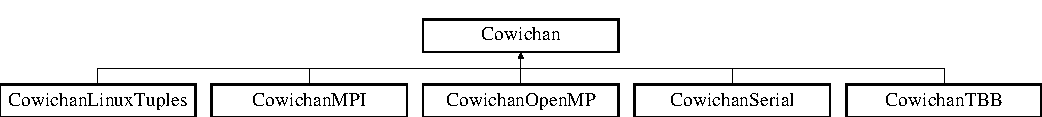
\includegraphics[height=1.56643cm]{class_cowichan}
\end{center}
\end{figure}
\subsection*{Public Member Functions}
\begin{CompactItemize}
\item 
{\footnotesize template$<$typename T $>$ }\\void \hyperlink{class_cowichan_14e706ef5a5f7661a623c595d7ed76f1}{print\_\-rect\_\-matrix} (T $\ast$matrix)
\item 
{\footnotesize template$<$typename T $>$ }\\void \hyperlink{class_cowichan_e8fdfb7dd3e8be0a7e9dbc531b1298d2}{print\_\-square\_\-matrix} (T $\ast$matrix)
\item 
{\footnotesize template$<$typename T $>$ }\\void \hyperlink{class_cowichan_90f1155f5c35308796b142b15d681a4b}{print\_\-vector} (T $\ast$vector)
\item 
void \hyperlink{class_cowichan_3b974ae1693ac661fb079b28981ca885}{print\_\-vector} (\hyperlink{class_point}{PointVector} points)
\item 
void \hyperlink{class_cowichan_905f3eb45f21cdaa1c32a421d001fa4c}{main} (int argc, char $\ast$argv\mbox{[}$\,$\mbox{]}, bool use\_\-randmat, bool use\_\-thresh)
\end{CompactItemize}
\subsection*{Protected Member Functions}
\begin{CompactItemize}
\item 
virtual void \hyperlink{class_cowichan_ec6cc4eb2ad444474b923532167e98a2}{mandel} (\hyperlink{cowichan_8hpp_82321152ddeeefe9c61350a42ed9e7af}{IntMatrix} matrix)=0
\item 
virtual void \hyperlink{class_cowichan_c44cacf9d9e363a5b076bcee8b9a7a73}{randmat} (\hyperlink{cowichan_8hpp_82321152ddeeefe9c61350a42ed9e7af}{IntMatrix} matrix)=0
\item 
virtual void \hyperlink{class_cowichan_308603053675bccbe631f04af921f57c}{half} (\hyperlink{cowichan_8hpp_82321152ddeeefe9c61350a42ed9e7af}{IntMatrix} matrixIn, \hyperlink{cowichan_8hpp_82321152ddeeefe9c61350a42ed9e7af}{IntMatrix} matrixOut)=0
\item 
virtual void \hyperlink{class_cowichan_ea126792a31e54a8722663b7ea768955}{invperc} (\hyperlink{cowichan_8hpp_82321152ddeeefe9c61350a42ed9e7af}{IntMatrix} matrix, \hyperlink{cowichan_8hpp_a64c8df2f1e9c8ea68a7bcc19aca683e}{BoolMatrix} mask)=0
\item 
virtual void \hyperlink{class_cowichan_a0b633b8c1f21884e0998a9c7020c08c}{thresh} (\hyperlink{cowichan_8hpp_82321152ddeeefe9c61350a42ed9e7af}{IntMatrix} matrix, \hyperlink{cowichan_8hpp_a64c8df2f1e9c8ea68a7bcc19aca683e}{BoolMatrix} mask)=0
\item 
virtual void \hyperlink{class_cowichan_d449595ef2fe934bdd128ac8b1f51d07}{life} (\hyperlink{cowichan_8hpp_a64c8df2f1e9c8ea68a7bcc19aca683e}{BoolMatrix} matrixIn, \hyperlink{cowichan_8hpp_a64c8df2f1e9c8ea68a7bcc19aca683e}{BoolMatrix} matrixOut)=0
\item 
virtual void \hyperlink{class_cowichan_13d60e06ced3b5da79d62c133ce82337}{winnow} (\hyperlink{cowichan_8hpp_82321152ddeeefe9c61350a42ed9e7af}{IntMatrix} matrix, \hyperlink{cowichan_8hpp_a64c8df2f1e9c8ea68a7bcc19aca683e}{BoolMatrix} mask, \hyperlink{class_point}{PointVector} points)=0
\item 
virtual void \hyperlink{class_cowichan_3df21e3c627958114e045c3559a29f30}{norm} (\hyperlink{class_point}{PointVector} pointsIn, \hyperlink{class_point}{PointVector} pointsOut)=0
\item 
virtual void \hyperlink{class_cowichan_0c6b68ae3c059b66893405f8530a2e0a}{hull} (\hyperlink{class_point}{PointVector} pointsIn, \hyperlink{class_point}{PointVector} pointsOut)=0
\item 
virtual void \hyperlink{class_cowichan_52f17221019290b88334b0ca7f3bcdb9}{outer} (\hyperlink{class_point}{PointVector} points, \hyperlink{cowichan_8hpp_3fb46f939e55c239fbc95656fc0f3399}{Matrix} matrix, \hyperlink{cowichan_8hpp_02bc1553e241b9b33408482658b3c355}{Vector} vector)=0
\item 
virtual void \hyperlink{class_cowichan_aa9aac74b96dc5ed33e821d94649d1b2}{gauss} (\hyperlink{cowichan_8hpp_3fb46f939e55c239fbc95656fc0f3399}{Matrix} matrix, \hyperlink{cowichan_8hpp_02bc1553e241b9b33408482658b3c355}{Vector} target, \hyperlink{cowichan_8hpp_02bc1553e241b9b33408482658b3c355}{Vector} solution)=0
\item 
virtual void \hyperlink{class_cowichan_92d8d9ae77208115fdfe69e1174f601c}{sor} (\hyperlink{cowichan_8hpp_3fb46f939e55c239fbc95656fc0f3399}{Matrix} matrix, \hyperlink{cowichan_8hpp_02bc1553e241b9b33408482658b3c355}{Vector} target, \hyperlink{cowichan_8hpp_02bc1553e241b9b33408482658b3c355}{Vector} solution)=0
\item 
virtual void \hyperlink{class_cowichan_3d7d4b581a1d6f0392dc452830fb3b03}{product} (\hyperlink{cowichan_8hpp_3fb46f939e55c239fbc95656fc0f3399}{Matrix} matrix, \hyperlink{cowichan_8hpp_02bc1553e241b9b33408482658b3c355}{Vector} candidate, \hyperlink{cowichan_8hpp_02bc1553e241b9b33408482658b3c355}{Vector} solution)=0
\item 
virtual \hyperlink{cowichan_8hpp_4d521b2c54a1f6312cc8fa04827eaf98}{real} \hyperlink{class_cowichan_775d72b5e7d122f9f32555352278250e}{vecdiff} (\hyperlink{cowichan_8hpp_02bc1553e241b9b33408482658b3c355}{Vector} actual, \hyperlink{cowichan_8hpp_02bc1553e241b9b33408482658b3c355}{Vector} computed)=0
\end{CompactItemize}
\subsection*{Protected Attributes}
\begin{CompactItemize}
\item 
\hyperlink{cowichan_8hpp_5b04577d5d21124855deaad298595371}{index\_\-t} \hyperlink{class_cowichan_44f139040042cc616e542be6faa28672}{nr}
\item 
\hyperlink{cowichan_8hpp_5b04577d5d21124855deaad298595371}{index\_\-t} \hyperlink{class_cowichan_81d2fc0da7b4ef388a1dbf08ac820eb1}{nc}
\item 
\hyperlink{cowichan_8hpp_5b04577d5d21124855deaad298595371}{index\_\-t} \hyperlink{class_cowichan_10e0c7c7bcccf11869821fa03cb7a6ee}{n}
\item 
\hyperlink{cowichan_8hpp_5b04577d5d21124855deaad298595371}{index\_\-t} \hyperlink{class_cowichan_edeb55a8b961f270ec35869dbba3afde}{lifeIterations}
\item 
\hyperlink{cowichan_8hpp_4d521b2c54a1f6312cc8fa04827eaf98}{real} \hyperlink{class_cowichan_f0bab1165abe53fea17e65764d247786}{mandelX0}
\item 
\hyperlink{cowichan_8hpp_4d521b2c54a1f6312cc8fa04827eaf98}{real} \hyperlink{class_cowichan_7b5e0e4e2026c78a6ec45fe306e5af93}{mandelY0}
\item 
\hyperlink{cowichan_8hpp_4d521b2c54a1f6312cc8fa04827eaf98}{real} \hyperlink{class_cowichan_edde2560c73a48dd44ea52c6a42c8649}{mandelDx}
\item 
\hyperlink{cowichan_8hpp_4d521b2c54a1f6312cc8fa04827eaf98}{real} \hyperlink{class_cowichan_7189d7127e740a2e6b14dcf0e757a500}{mandelDy}
\item 
\hyperlink{cowichan_8hpp_4d521b2c54a1f6312cc8fa04827eaf98}{real} \hyperlink{class_cowichan_a42c0ae639cc3ac124a013bc3e3162ad}{threshPercent}
\item 
\hyperlink{cowichan_8hpp_5b04577d5d21124855deaad298595371}{index\_\-t} \hyperlink{class_cowichan_c637b7380ab889ed42652790a3c542c6}{invpercNFill}
\item 
\hyperlink{cowichan_8hpp_c96945095fd0ce7186a1d00a89f77d2c}{INT\_\-TYPE} \hyperlink{class_cowichan_e9f8e9769f15e2648435064d4286b1a6}{seed}
\end{CompactItemize}
\subsection*{Static Protected Attributes}
\begin{CompactItemize}
\item 
static const char $\ast$ \hyperlink{class_cowichan_17937f5dfe24c46c00a76d48ca70ccaa}{CHAIN} = \char`\"{}chain\char`\"{}
\item 
static const char $\ast$ \hyperlink{class_cowichan_40d3f57ec83c7c1ec3af94c37d849049}{MANDEL} = \char`\"{}mandel\char`\"{}
\item 
static const char $\ast$ \hyperlink{class_cowichan_c9e66484bf3be07bfeac5511f514f102}{RANDMAT} = \char`\"{}randmat\char`\"{}
\item 
static const char $\ast$ \hyperlink{class_cowichan_6ef0b7dddca7331c9bfb2acd0ea60088}{HALF} = \char`\"{}half\char`\"{}
\item 
static const char $\ast$ \hyperlink{class_cowichan_0665b5094fb551e4f000502ec752a4e8}{INVPERC} = \char`\"{}invperc\char`\"{}
\item 
static const char $\ast$ \hyperlink{class_cowichan_e7adc012eb484f209b869db5062dacd0}{THRESH} = \char`\"{}thresh\char`\"{}
\item 
static const char $\ast$ \hyperlink{class_cowichan_6d8355328c9a2e36321d3d33930f56b2}{LIFE} = \char`\"{}life\char`\"{}
\item 
static const char $\ast$ \hyperlink{class_cowichan_a4d4acfeeb50c0552487a59a58b3f962}{WINNOW} = \char`\"{}winnow\char`\"{}
\item 
static const char $\ast$ \hyperlink{class_cowichan_4e2cd818307d1e806861489216e74a0f}{NORM} = \char`\"{}norm\char`\"{}
\item 
static const char $\ast$ \hyperlink{class_cowichan_c0ca862afefd5d6ab8fefdbf47428b21}{HULL} = \char`\"{}hull\char`\"{}
\item 
static const char $\ast$ \hyperlink{class_cowichan_b858724b8531751af4f611b978998be4}{OUTER} = \char`\"{}outer\char`\"{}
\item 
static const char $\ast$ \hyperlink{class_cowichan_b51b18cab3bd7cab0f3eb5c10f4cce0a}{GAUSS} = \char`\"{}gauss\char`\"{}
\item 
static const char $\ast$ \hyperlink{class_cowichan_eaac49e2ebb0c5149506f0544cd87794}{SOR} = \char`\"{}sor\char`\"{}
\item 
static const char $\ast$ \hyperlink{class_cowichan_57a1deea813a95ad7ed5a46dd000e576}{PRODUCT} = \char`\"{}product\char`\"{}
\item 
static const char $\ast$ \hyperlink{class_cowichan_d70f851efe3d20a89d7bcf5e7db70344}{VECDIFF} = \char`\"{}vecdiff\char`\"{}
\end{CompactItemize}
\subsection*{Private Member Functions}
\begin{CompactItemize}
\item 
void \hyperlink{class_cowichan_08ee88eb612571e8faa20b2645dc906d}{chain} (bool use\_\-randmat, bool use\_\-thresh)
\end{CompactItemize}


\subsection{Detailed Description}
Base class for all C++ implementations. 

The abstract class containing the inputs, definitions, and some debugging methods for the \hyperlink{class_cowichan}{Cowichan} problems. 

\subsection{Member Function Documentation}
\hypertarget{class_cowichan_08ee88eb612571e8faa20b2645dc906d}{
\index{Cowichan@{Cowichan}!chain@{chain}}
\index{chain@{chain}!Cowichan@{Cowichan}}
\subsubsection[{chain}]{\setlength{\rightskip}{0pt plus 5cm}void Cowichan::chain (bool {\em use\_\-randmat}, \/  bool {\em use\_\-thresh})\hspace{0.3cm}{\tt  \mbox{[}private\mbox{]}}}}
\label{class_cowichan_08ee88eb612571e8faa20b2645dc906d}


Runs the cowichan problem set, chained together. The order in the chain is: \begin{enumerate}
\item \hyperlink{class_cowichan_c44cacf9d9e363a5b076bcee8b9a7a73}{Cowichan::randmat} or \hyperlink{class_cowichan_ec6cc4eb2ad444474b923532167e98a2}{Cowichan::mandel} \item \hyperlink{class_cowichan_308603053675bccbe631f04af921f57c}{Cowichan::half} \item \hyperlink{class_cowichan_ea126792a31e54a8722663b7ea768955}{Cowichan::invperc} or \hyperlink{class_cowichan_a0b633b8c1f21884e0998a9c7020c08c}{Cowichan::thresh} \item \hyperlink{class_cowichan_d449595ef2fe934bdd128ac8b1f51d07}{Cowichan::life} \item \hyperlink{class_cowichan_13d60e06ced3b5da79d62c133ce82337}{Cowichan::winnow} \item \hyperlink{class_cowichan_3df21e3c627958114e045c3559a29f30}{Cowichan::norm} \item \hyperlink{class_cowichan_0c6b68ae3c059b66893405f8530a2e0a}{Cowichan::hull} \item \hyperlink{class_cowichan_52f17221019290b88334b0ca7f3bcdb9}{Cowichan::outer} \item \hyperlink{class_cowichan_aa9aac74b96dc5ed33e821d94649d1b2}{Cowichan::gauss} \item \hyperlink{class_cowichan_92d8d9ae77208115fdfe69e1174f601c}{Cowichan::sor} \item \hyperlink{class_cowichan_3d7d4b581a1d6f0392dc452830fb3b03}{Cowichan::product} (for gauss) \item \hyperlink{class_cowichan_3d7d4b581a1d6f0392dc452830fb3b03}{Cowichan::product} (for sor) \item \hyperlink{class_cowichan_775d72b5e7d122f9f32555352278250e}{Cowichan::vecdiff} \end{enumerate}
\begin{Desc}
\item[Parameters:]
\begin{description}
\item[{\em use\_\-randmat}]in step 1 use: randmat (if true) or mandel (if false). \item[{\em use\_\-thresh}]in step 3 use: thresh (if true) or invperc (if false). \end{description}
\end{Desc}


Reimplemented in \hyperlink{class_cowichan_linux_tuples_fd49b2a0af64bafb93a5fe1210c68acd}{CowichanLinuxTuples}.\hypertarget{class_cowichan_aa9aac74b96dc5ed33e821d94649d1b2}{
\index{Cowichan@{Cowichan}!gauss@{gauss}}
\index{gauss@{gauss}!Cowichan@{Cowichan}}
\subsubsection[{gauss}]{\setlength{\rightskip}{0pt plus 5cm}virtual void Cowichan::gauss ({\bf Matrix} {\em matrix}, \/  {\bf Vector} {\em target}, \/  {\bf Vector} {\em solution})\hspace{0.3cm}{\tt  \mbox{[}protected, pure virtual\mbox{]}}}}
\label{class_cowichan_aa9aac74b96dc5ed33e821d94649d1b2}


For description see \hyperlink{index_gauss_sec}{11. Gaussian Elimination} \begin{Desc}
\item[Parameters:]
\begin{description}
\item[{\em matrix}]matrix A in AX = V. \item[{\em target}]vector V in AX = V. \item[{\em solution}]vector X in AX = V. \end{description}
\end{Desc}


Implemented in \hyperlink{class_cowichan_serial_b196d2384c2fe8b185e6269a050399eb}{CowichanSerial}, \hyperlink{class_cowichan_open_m_p_363bcd6f0c7b4d0fced94fe4cd59a267}{CowichanOpenMP}, \hyperlink{class_cowichan_t_b_b_d51868e0e65482f7c9e69d73b3904822}{CowichanTBB}, \hyperlink{class_cowichan_m_p_i_975f8da6c166fe1db3cf9341eeaab000}{CowichanMPI}, and \hyperlink{class_cowichan_linux_tuples_fd3e659afb38415f56fd508333b7bb1b}{CowichanLinuxTuples}.\hypertarget{class_cowichan_308603053675bccbe631f04af921f57c}{
\index{Cowichan@{Cowichan}!half@{half}}
\index{half@{half}!Cowichan@{Cowichan}}
\subsubsection[{half}]{\setlength{\rightskip}{0pt plus 5cm}virtual void Cowichan::half ({\bf IntMatrix} {\em matrixIn}, \/  {\bf IntMatrix} {\em matrixOut})\hspace{0.3cm}{\tt  \mbox{[}protected, pure virtual\mbox{]}}}}
\label{class_cowichan_308603053675bccbe631f04af921f57c}


For description see \hyperlink{index_half_sec}{3. Two-Dimensional Shuffle} \begin{Desc}
\item[Parameters:]
\begin{description}
\item[{\em matrixIn}]matrix to shuffle. \item[{\em matrixOut}]shuffled matrix. \end{description}
\end{Desc}


Implemented in \hyperlink{class_cowichan_serial_c08a6b3e23ce26959bac12af077f924f}{CowichanSerial}, \hyperlink{class_cowichan_open_m_p_70989ffe182aebf590e39c56e146b0fb}{CowichanOpenMP}, \hyperlink{class_cowichan_t_b_b_bbf17e641657d54fc0c571c008ac8f7a}{CowichanTBB}, \hyperlink{class_cowichan_m_p_i_154bbd1a400ee4571f761bff1cdf67cd}{CowichanMPI}, and \hyperlink{class_cowichan_linux_tuples_f3bd58ad2653f06d242d473e7bffda0b}{CowichanLinuxTuples}.\hypertarget{class_cowichan_0c6b68ae3c059b66893405f8530a2e0a}{
\index{Cowichan@{Cowichan}!hull@{hull}}
\index{hull@{hull}!Cowichan@{Cowichan}}
\subsubsection[{hull}]{\setlength{\rightskip}{0pt plus 5cm}virtual void Cowichan::hull ({\bf PointVector} {\em pointsIn}, \/  {\bf PointVector} {\em pointsOut})\hspace{0.3cm}{\tt  \mbox{[}protected, pure virtual\mbox{]}}}}
\label{class_cowichan_0c6b68ae3c059b66893405f8530a2e0a}


For description see \hyperlink{index_hull_sec}{9. Convex Hull} \begin{Desc}
\item[Parameters:]
\begin{description}
\item[{\em pointsIn}]points to run convex hull on. \item[{\em pointsOut}]reordered points from pointsIn. \end{description}
\end{Desc}


Implemented in \hyperlink{class_cowichan_serial_e75cedf0a296dd7ad3dc41cadc51776f}{CowichanSerial}, \hyperlink{class_cowichan_open_m_p_cb444dd3e2c0f1f27f4135de0279d09e}{CowichanOpenMP}, \hyperlink{class_cowichan_t_b_b_0d23aa05dc21fd9e8b033769097b4b18}{CowichanTBB}, \hyperlink{class_cowichan_m_p_i_22b3dce35fd93635bd4c1596e7fb839c}{CowichanMPI}, and \hyperlink{class_cowichan_linux_tuples_501f87594d62af261ff0b1954a60ddc4}{CowichanLinuxTuples}.\hypertarget{class_cowichan_ea126792a31e54a8722663b7ea768955}{
\index{Cowichan@{Cowichan}!invperc@{invperc}}
\index{invperc@{invperc}!Cowichan@{Cowichan}}
\subsubsection[{invperc}]{\setlength{\rightskip}{0pt plus 5cm}virtual void Cowichan::invperc ({\bf IntMatrix} {\em matrix}, \/  {\bf BoolMatrix} {\em mask})\hspace{0.3cm}{\tt  \mbox{[}protected, pure virtual\mbox{]}}}}
\label{class_cowichan_ea126792a31e54a8722663b7ea768955}


For description see \hyperlink{index_invperc_sec}{4. Invasion Percolation} \begin{Desc}
\item[Parameters:]
\begin{description}
\item[{\em matrix}]filling resistance matrix. \item[{\em mask}]filled cells. \end{description}
\end{Desc}


Implemented in \hyperlink{class_cowichan_serial_9b1cf3fcbb40498609826433b8ea2f6a}{CowichanSerial}, \hyperlink{class_cowichan_open_m_p_4824c6b8509b5da835fbc5f64eb3e063}{CowichanOpenMP}, \hyperlink{class_cowichan_t_b_b_e4f9f8c31feea9b3a167fc2880a97610}{CowichanTBB}, \hyperlink{class_cowichan_m_p_i_bcd0f18fcccc8973ddaacf4dda190b53}{CowichanMPI}, and \hyperlink{class_cowichan_linux_tuples_5497a17a63cc5faad7afa54d013ea741}{CowichanLinuxTuples}.\hypertarget{class_cowichan_d449595ef2fe934bdd128ac8b1f51d07}{
\index{Cowichan@{Cowichan}!life@{life}}
\index{life@{life}!Cowichan@{Cowichan}}
\subsubsection[{life}]{\setlength{\rightskip}{0pt plus 5cm}virtual void Cowichan::life ({\bf BoolMatrix} {\em matrixIn}, \/  {\bf BoolMatrix} {\em matrixOut})\hspace{0.3cm}{\tt  \mbox{[}protected, pure virtual\mbox{]}}}}
\label{class_cowichan_d449595ef2fe934bdd128ac8b1f51d07}


For description see \hyperlink{index_life_sec}{6. Game of Life} \begin{Desc}
\item[Parameters:]
\begin{description}
\item[{\em matrixIn}]initial world. \item[{\em matrixOut}]final world. \end{description}
\end{Desc}


Implemented in \hyperlink{class_cowichan_serial_ffd5b022c1d24226e11924094d8af349}{CowichanSerial}, \hyperlink{class_cowichan_open_m_p_d24f3ef01289b8f1bd7b864f585daa62}{CowichanOpenMP}, \hyperlink{class_cowichan_t_b_b_273e3e8a2e05108f59ec613472bfa363}{CowichanTBB}, \hyperlink{class_cowichan_m_p_i_9c739951d036ef7905bda7cb896e0edf}{CowichanMPI}, and \hyperlink{class_cowichan_linux_tuples_967138bbdead76eec50f31465dd9d5f1}{CowichanLinuxTuples}.\hypertarget{class_cowichan_905f3eb45f21cdaa1c32a421d001fa4c}{
\index{Cowichan@{Cowichan}!main@{main}}
\index{main@{main}!Cowichan@{Cowichan}}
\subsubsection[{main}]{\setlength{\rightskip}{0pt plus 5cm}void Cowichan::main (int {\em argc}, \/  char $\ast$ {\em argv}\mbox{[}$\,$\mbox{]}, \/  bool {\em use\_\-randmat}, \/  bool {\em use\_\-thresh})}}
\label{class_cowichan_905f3eb45f21cdaa1c32a421d001fa4c}


Runs cowichan problems based on command line input. Problem name can be specified on the command line. Otherwise, the chained version is run. \begin{Desc}
\item[See also:]\hyperlink{class_cowichan_08ee88eb612571e8faa20b2645dc906d}{Cowichan::chain} \end{Desc}
\begin{Desc}
\item[Parameters:]
\begin{description}
\item[{\em argc}]number of command line arguments. \item[{\em argv}]command line arguments. \item[{\em use\_\-randmat}]passed to chain if chained version is used. \item[{\em use\_\-thresh}]passed to chain if chained version is used. \end{description}
\end{Desc}
\hypertarget{class_cowichan_ec6cc4eb2ad444474b923532167e98a2}{
\index{Cowichan@{Cowichan}!mandel@{mandel}}
\index{mandel@{mandel}!Cowichan@{Cowichan}}
\subsubsection[{mandel}]{\setlength{\rightskip}{0pt plus 5cm}virtual void Cowichan::mandel ({\bf IntMatrix} {\em matrix})\hspace{0.3cm}{\tt  \mbox{[}protected, pure virtual\mbox{]}}}}
\label{class_cowichan_ec6cc4eb2ad444474b923532167e98a2}


For description see \hyperlink{index_mandel_sec}{1. Mandelbrot Set Generation} \begin{Desc}
\item[Parameters:]
\begin{description}
\item[{\em matrix}]matrix to fill. \end{description}
\end{Desc}


Implemented in \hyperlink{class_cowichan_serial_97a58b7901d8a7680cc28d42cb94d532}{CowichanSerial}, \hyperlink{class_cowichan_open_m_p_6809c2738792de047ee59259636c1afd}{CowichanOpenMP}, \hyperlink{class_cowichan_t_b_b_1e58b60ff22a58aba69567ecc6740878}{CowichanTBB}, \hyperlink{class_cowichan_m_p_i_58274fc55ed8a352a8924b130f3b5d2e}{CowichanMPI}, and \hyperlink{class_cowichan_linux_tuples_8774404842868381379ec627e8373cec}{CowichanLinuxTuples}.\hypertarget{class_cowichan_3df21e3c627958114e045c3559a29f30}{
\index{Cowichan@{Cowichan}!norm@{norm}}
\index{norm@{norm}!Cowichan@{Cowichan}}
\subsubsection[{norm}]{\setlength{\rightskip}{0pt plus 5cm}virtual void Cowichan::norm ({\bf PointVector} {\em pointsIn}, \/  {\bf PointVector} {\em pointsOut})\hspace{0.3cm}{\tt  \mbox{[}protected, pure virtual\mbox{]}}}}
\label{class_cowichan_3df21e3c627958114e045c3559a29f30}


For description see \hyperlink{index_norm_sec}{8. Point Location Normalization} \begin{Desc}
\item[Parameters:]
\begin{description}
\item[{\em pointsIn}]points to normalize. \item[{\em pointsOut}]normalized points. \end{description}
\end{Desc}


Implemented in \hyperlink{class_cowichan_serial_0eeb47447c6a6b94ff7c6999c96fda0e}{CowichanSerial}, \hyperlink{class_cowichan_open_m_p_4ffbe36816235bc6abec30eae2be2d78}{CowichanOpenMP}, \hyperlink{class_cowichan_t_b_b_ca08645b51a242317a115cd7ce7d81fe}{CowichanTBB}, \hyperlink{class_cowichan_m_p_i_11df49e804427d4a0d085f4cff9302d0}{CowichanMPI}, and \hyperlink{class_cowichan_linux_tuples_922209c219bb5b9268263dae4000ea81}{CowichanLinuxTuples}.\hypertarget{class_cowichan_52f17221019290b88334b0ca7f3bcdb9}{
\index{Cowichan@{Cowichan}!outer@{outer}}
\index{outer@{outer}!Cowichan@{Cowichan}}
\subsubsection[{outer}]{\setlength{\rightskip}{0pt plus 5cm}virtual void Cowichan::outer ({\bf PointVector} {\em points}, \/  {\bf Matrix} {\em matrix}, \/  {\bf Vector} {\em vector})\hspace{0.3cm}{\tt  \mbox{[}protected, pure virtual\mbox{]}}}}
\label{class_cowichan_52f17221019290b88334b0ca7f3bcdb9}


For description see \hyperlink{index_outer_sec}{10. Outer Product} \begin{Desc}
\item[Parameters:]
\begin{description}
\item[{\em points}]vector of points. \item[{\em matrix}]resulting distance matrix. \item[{\em vector}]resulting distance vector. \end{description}
\end{Desc}


Implemented in \hyperlink{class_cowichan_serial_05f6899081a457d58978e4f6bda2db6a}{CowichanSerial}, \hyperlink{class_cowichan_open_m_p_99a0570f754ac82968d73093476de533}{CowichanOpenMP}, \hyperlink{class_cowichan_t_b_b_92a763b9733cdcceda13b7b7ea0bc229}{CowichanTBB}, \hyperlink{class_cowichan_m_p_i_39fcc8a331b0e26438fbf43fa01cf7c1}{CowichanMPI}, and \hyperlink{class_cowichan_linux_tuples_b16e1c3b60f920c12460a74289558dcb}{CowichanLinuxTuples}.\hypertarget{class_cowichan_14e706ef5a5f7661a623c595d7ed76f1}{
\index{Cowichan@{Cowichan}!print\_\-rect\_\-matrix@{print\_\-rect\_\-matrix}}
\index{print\_\-rect\_\-matrix@{print\_\-rect\_\-matrix}!Cowichan@{Cowichan}}
\subsubsection[{print\_\-rect\_\-matrix}]{\setlength{\rightskip}{0pt plus 5cm}template$<$typename T $>$ void Cowichan::print\_\-rect\_\-matrix (T $\ast$ {\em matrix})\hspace{0.3cm}{\tt  \mbox{[}inline\mbox{]}}}}
\label{class_cowichan_14e706ef5a5f7661a623c595d7ed76f1}


DEBUGGING FUNCTION: Print a rectangular matrix on std::cout. \begin{Desc}
\item[Parameters:]
\begin{description}
\item[{\em matrix}]matrix to print. \end{description}
\end{Desc}
\hypertarget{class_cowichan_e8fdfb7dd3e8be0a7e9dbc531b1298d2}{
\index{Cowichan@{Cowichan}!print\_\-square\_\-matrix@{print\_\-square\_\-matrix}}
\index{print\_\-square\_\-matrix@{print\_\-square\_\-matrix}!Cowichan@{Cowichan}}
\subsubsection[{print\_\-square\_\-matrix}]{\setlength{\rightskip}{0pt plus 5cm}template$<$typename T $>$ void Cowichan::print\_\-square\_\-matrix (T $\ast$ {\em matrix})\hspace{0.3cm}{\tt  \mbox{[}inline\mbox{]}}}}
\label{class_cowichan_e8fdfb7dd3e8be0a7e9dbc531b1298d2}


DEBUGGING FUNCTION: Print a square matrix on std::cout. \begin{Desc}
\item[Parameters:]
\begin{description}
\item[{\em matrix}]matrix to print. \end{description}
\end{Desc}
\hypertarget{class_cowichan_3b974ae1693ac661fb079b28981ca885}{
\index{Cowichan@{Cowichan}!print\_\-vector@{print\_\-vector}}
\index{print\_\-vector@{print\_\-vector}!Cowichan@{Cowichan}}
\subsubsection[{print\_\-vector}]{\setlength{\rightskip}{0pt plus 5cm}void Cowichan::print\_\-vector ({\bf PointVector} {\em points})}}
\label{class_cowichan_3b974ae1693ac661fb079b28981ca885}


DEBUGGING FUNCTION: Print a point vector. \begin{Desc}
\item[Parameters:]
\begin{description}
\item[{\em points}]vector of points to print. \end{description}
\end{Desc}
\hypertarget{class_cowichan_90f1155f5c35308796b142b15d681a4b}{
\index{Cowichan@{Cowichan}!print\_\-vector@{print\_\-vector}}
\index{print\_\-vector@{print\_\-vector}!Cowichan@{Cowichan}}
\subsubsection[{print\_\-vector}]{\setlength{\rightskip}{0pt plus 5cm}template$<$typename T $>$ void Cowichan::print\_\-vector (T $\ast$ {\em vector})\hspace{0.3cm}{\tt  \mbox{[}inline\mbox{]}}}}
\label{class_cowichan_90f1155f5c35308796b142b15d681a4b}


DEBUGGING FUNCTION: Print a vector on std::cout. \begin{Desc}
\item[Parameters:]
\begin{description}
\item[{\em vector}]vector to print. \end{description}
\end{Desc}
\hypertarget{class_cowichan_3d7d4b581a1d6f0392dc452830fb3b03}{
\index{Cowichan@{Cowichan}!product@{product}}
\index{product@{product}!Cowichan@{Cowichan}}
\subsubsection[{product}]{\setlength{\rightskip}{0pt plus 5cm}virtual void Cowichan::product ({\bf Matrix} {\em matrix}, \/  {\bf Vector} {\em candidate}, \/  {\bf Vector} {\em solution})\hspace{0.3cm}{\tt  \mbox{[}protected, pure virtual\mbox{]}}}}
\label{class_cowichan_3d7d4b581a1d6f0392dc452830fb3b03}


For description see \hyperlink{index_product_sec}{13. Matrix-Vector Product} \begin{Desc}
\item[Parameters:]
\begin{description}
\item[{\em matrix}]matrix A in AX = V. \item[{\em candidate}]vector X in AX = V. \item[{\em solution}]vector V in AX = V. \end{description}
\end{Desc}


Implemented in \hyperlink{class_cowichan_serial_00411b35445d7d3038b96d53e43bdffa}{CowichanSerial}, \hyperlink{class_cowichan_open_m_p_41d0067382570d1e784f62f2c5963d49}{CowichanOpenMP}, \hyperlink{class_cowichan_t_b_b_f3144458520e2dff1f9fad5753f6fc3d}{CowichanTBB}, \hyperlink{class_cowichan_m_p_i_1b7dccf774caccb26839cd29fe0a5cb0}{CowichanMPI}, and \hyperlink{class_cowichan_linux_tuples_c4874f09c54056ac94d00f9e341a94f4}{CowichanLinuxTuples}.\hypertarget{class_cowichan_c44cacf9d9e363a5b076bcee8b9a7a73}{
\index{Cowichan@{Cowichan}!randmat@{randmat}}
\index{randmat@{randmat}!Cowichan@{Cowichan}}
\subsubsection[{randmat}]{\setlength{\rightskip}{0pt plus 5cm}virtual void Cowichan::randmat ({\bf IntMatrix} {\em matrix})\hspace{0.3cm}{\tt  \mbox{[}protected, pure virtual\mbox{]}}}}
\label{class_cowichan_c44cacf9d9e363a5b076bcee8b9a7a73}


For description see \hyperlink{index_randmat_sec}{2. Random Number Generation} \begin{Desc}
\item[Parameters:]
\begin{description}
\item[{\em matrix}]matrix to fill. \end{description}
\end{Desc}


Implemented in \hyperlink{class_cowichan_serial_2d24c0e562f7b109ec2ed916f38e5911}{CowichanSerial}, \hyperlink{class_cowichan_open_m_p_2c7c4e4dd96f82b7280a412c1fceed2c}{CowichanOpenMP}, \hyperlink{class_cowichan_t_b_b_b9b5cb4b4b5dc8907b2a01825cd4aaff}{CowichanTBB}, \hyperlink{class_cowichan_m_p_i_6805f21144aeaeddc4549e1b2b42bca8}{CowichanMPI}, and \hyperlink{class_cowichan_linux_tuples_ff90c6a27db51366570b70d352de7fab}{CowichanLinuxTuples}.\hypertarget{class_cowichan_92d8d9ae77208115fdfe69e1174f601c}{
\index{Cowichan@{Cowichan}!sor@{sor}}
\index{sor@{sor}!Cowichan@{Cowichan}}
\subsubsection[{sor}]{\setlength{\rightskip}{0pt plus 5cm}virtual void Cowichan::sor ({\bf Matrix} {\em matrix}, \/  {\bf Vector} {\em target}, \/  {\bf Vector} {\em solution})\hspace{0.3cm}{\tt  \mbox{[}protected, pure virtual\mbox{]}}}}
\label{class_cowichan_92d8d9ae77208115fdfe69e1174f601c}


For description see \hyperlink{index_sor_sec}{12. Successive Over-Relaxation} \begin{Desc}
\item[Parameters:]
\begin{description}
\item[{\em matrix}]matrix A in AX = V. \item[{\em target}]vector V in AX = V. \item[{\em solution}]vector X in AX = V. \end{description}
\end{Desc}


Implemented in \hyperlink{class_cowichan_serial_6e8b06711d976de1adc1e4dc81e560e5}{CowichanSerial}, \hyperlink{class_cowichan_open_m_p_d6482d0369a26a51ef0e37ab238fc664}{CowichanOpenMP}, \hyperlink{class_cowichan_t_b_b_dbb32ce457d0edca6815ab1cb2459276}{CowichanTBB}, \hyperlink{class_cowichan_m_p_i_7388c844e8aa73ab0923443a3a7ef069}{CowichanMPI}, and \hyperlink{class_cowichan_linux_tuples_aa2c469c3f520a5a56c5ec1ac9a5a6c6}{CowichanLinuxTuples}.\hypertarget{class_cowichan_a0b633b8c1f21884e0998a9c7020c08c}{
\index{Cowichan@{Cowichan}!thresh@{thresh}}
\index{thresh@{thresh}!Cowichan@{Cowichan}}
\subsubsection[{thresh}]{\setlength{\rightskip}{0pt plus 5cm}virtual void Cowichan::thresh ({\bf IntMatrix} {\em matrix}, \/  {\bf BoolMatrix} {\em mask})\hspace{0.3cm}{\tt  \mbox{[}protected, pure virtual\mbox{]}}}}
\label{class_cowichan_a0b633b8c1f21884e0998a9c7020c08c}


For description see \hyperlink{index_thresh_sec}{5. Histogram Thresholding} \begin{Desc}
\item[Parameters:]
\begin{description}
\item[{\em matrix}]image. \item[{\em mask}]image after thresholding. \end{description}
\end{Desc}


Implemented in \hyperlink{class_cowichan_serial_7c0f93b2099ce919f91b5d953ff76511}{CowichanSerial}, \hyperlink{class_cowichan_open_m_p_e72c4c0a162f30eac37333bd28db97bc}{CowichanOpenMP}, \hyperlink{class_cowichan_t_b_b_3306d21f0b3d12cc2e3b050b99812a27}{CowichanTBB}, \hyperlink{class_cowichan_m_p_i_49ff96b091a61e9cfd9aad8824e7fbbd}{CowichanMPI}, and \hyperlink{class_cowichan_linux_tuples_b8cf055ec3d42a1ccde6d818c5a43a74}{CowichanLinuxTuples}.\hypertarget{class_cowichan_775d72b5e7d122f9f32555352278250e}{
\index{Cowichan@{Cowichan}!vecdiff@{vecdiff}}
\index{vecdiff@{vecdiff}!Cowichan@{Cowichan}}
\subsubsection[{vecdiff}]{\setlength{\rightskip}{0pt plus 5cm}virtual {\bf real} Cowichan::vecdiff ({\bf Vector} {\em actual}, \/  {\bf Vector} {\em computed})\hspace{0.3cm}{\tt  \mbox{[}protected, pure virtual\mbox{]}}}}
\label{class_cowichan_775d72b5e7d122f9f32555352278250e}


For description see \hyperlink{index_vecdiff_sec}{14. 1-Norm Vector Difference} \begin{Desc}
\item[Parameters:]
\begin{description}
\item[{\em actual}]first vector. \item[{\em computed}]second vector. \end{description}
\end{Desc}


Implemented in \hyperlink{class_cowichan_serial_34b75a2084051b3677071bb3c334d1f4}{CowichanSerial}, \hyperlink{class_cowichan_open_m_p_92aa23ed47da0a5a3b43416ab08199b3}{CowichanOpenMP}, \hyperlink{class_cowichan_t_b_b_28c976743df231fd183e4db9306050b1}{CowichanTBB}, \hyperlink{class_cowichan_m_p_i_c5470a2876efecf843b19c37c21ecf19}{CowichanMPI}, and \hyperlink{class_cowichan_linux_tuples_213185666ea7dd0c9abc59899b454086}{CowichanLinuxTuples}.\hypertarget{class_cowichan_13d60e06ced3b5da79d62c133ce82337}{
\index{Cowichan@{Cowichan}!winnow@{winnow}}
\index{winnow@{winnow}!Cowichan@{Cowichan}}
\subsubsection[{winnow}]{\setlength{\rightskip}{0pt plus 5cm}virtual void Cowichan::winnow ({\bf IntMatrix} {\em matrix}, \/  {\bf BoolMatrix} {\em mask}, \/  {\bf PointVector} {\em points})\hspace{0.3cm}{\tt  \mbox{[}protected, pure virtual\mbox{]}}}}
\label{class_cowichan_13d60e06ced3b5da79d62c133ce82337}


For description see \hyperlink{index_winnow_sec}{7. Weighted Point Selection} \begin{Desc}
\item[Parameters:]
\begin{description}
\item[{\em matrix}]integer matrix. \item[{\em mask}]boolean matrix. \item[{\em points}]evenly selected points. \end{description}
\end{Desc}


Implemented in \hyperlink{class_cowichan_serial_33daca65431f792c2f4f0e7f8d29fa01}{CowichanSerial}, \hyperlink{class_cowichan_open_m_p_4a518f2b5590d4acd670f333471a380a}{CowichanOpenMP}, \hyperlink{class_cowichan_t_b_b_77178470ef780e0505137dc1d22a85a2}{CowichanTBB}, \hyperlink{class_cowichan_m_p_i_9be48d86fc51ce13ef79d5fe2c8a16e0}{CowichanMPI}, and \hyperlink{class_cowichan_linux_tuples_2b1a77ecbd01ec847cf63fe7ebb50e35}{CowichanLinuxTuples}.

\subsection{Member Data Documentation}
\hypertarget{class_cowichan_17937f5dfe24c46c00a76d48ca70ccaa}{
\index{Cowichan@{Cowichan}!CHAIN@{CHAIN}}
\index{CHAIN@{CHAIN}!Cowichan@{Cowichan}}
\subsubsection[{CHAIN}]{\setlength{\rightskip}{0pt plus 5cm}const char $\ast$ {\bf Cowichan::CHAIN} = \char`\"{}chain\char`\"{}\hspace{0.3cm}{\tt  \mbox{[}static, protected\mbox{]}}}}
\label{class_cowichan_17937f5dfe24c46c00a76d48ca70ccaa}


Name for chain. \hypertarget{class_cowichan_b51b18cab3bd7cab0f3eb5c10f4cce0a}{
\index{Cowichan@{Cowichan}!GAUSS@{GAUSS}}
\index{GAUSS@{GAUSS}!Cowichan@{Cowichan}}
\subsubsection[{GAUSS}]{\setlength{\rightskip}{0pt plus 5cm}const char $\ast$ {\bf Cowichan::GAUSS} = \char`\"{}gauss\char`\"{}\hspace{0.3cm}{\tt  \mbox{[}static, protected\mbox{]}}}}
\label{class_cowichan_b51b18cab3bd7cab0f3eb5c10f4cce0a}


Name for gauss. \hypertarget{class_cowichan_6ef0b7dddca7331c9bfb2acd0ea60088}{
\index{Cowichan@{Cowichan}!HALF@{HALF}}
\index{HALF@{HALF}!Cowichan@{Cowichan}}
\subsubsection[{HALF}]{\setlength{\rightskip}{0pt plus 5cm}const char $\ast$ {\bf Cowichan::HALF} = \char`\"{}half\char`\"{}\hspace{0.3cm}{\tt  \mbox{[}static, protected\mbox{]}}}}
\label{class_cowichan_6ef0b7dddca7331c9bfb2acd0ea60088}


Name for half. \hypertarget{class_cowichan_c0ca862afefd5d6ab8fefdbf47428b21}{
\index{Cowichan@{Cowichan}!HULL@{HULL}}
\index{HULL@{HULL}!Cowichan@{Cowichan}}
\subsubsection[{HULL}]{\setlength{\rightskip}{0pt plus 5cm}const char $\ast$ {\bf Cowichan::HULL} = \char`\"{}hull\char`\"{}\hspace{0.3cm}{\tt  \mbox{[}static, protected\mbox{]}}}}
\label{class_cowichan_c0ca862afefd5d6ab8fefdbf47428b21}


Name for hull. \hypertarget{class_cowichan_0665b5094fb551e4f000502ec752a4e8}{
\index{Cowichan@{Cowichan}!INVPERC@{INVPERC}}
\index{INVPERC@{INVPERC}!Cowichan@{Cowichan}}
\subsubsection[{INVPERC}]{\setlength{\rightskip}{0pt plus 5cm}const char $\ast$ {\bf Cowichan::INVPERC} = \char`\"{}invperc\char`\"{}\hspace{0.3cm}{\tt  \mbox{[}static, protected\mbox{]}}}}
\label{class_cowichan_0665b5094fb551e4f000502ec752a4e8}


Name for invperc. \hypertarget{class_cowichan_c637b7380ab889ed42652790a3c542c6}{
\index{Cowichan@{Cowichan}!invpercNFill@{invpercNFill}}
\index{invpercNFill@{invpercNFill}!Cowichan@{Cowichan}}
\subsubsection[{invpercNFill}]{\setlength{\rightskip}{0pt plus 5cm}{\bf index\_\-t} {\bf Cowichan::invpercNFill}\hspace{0.3cm}{\tt  \mbox{[}protected\mbox{]}}}}
\label{class_cowichan_c637b7380ab889ed42652790a3c542c6}


Number of cells to fill. \hypertarget{class_cowichan_6d8355328c9a2e36321d3d33930f56b2}{
\index{Cowichan@{Cowichan}!LIFE@{LIFE}}
\index{LIFE@{LIFE}!Cowichan@{Cowichan}}
\subsubsection[{LIFE}]{\setlength{\rightskip}{0pt plus 5cm}const char $\ast$ {\bf Cowichan::LIFE} = \char`\"{}life\char`\"{}\hspace{0.3cm}{\tt  \mbox{[}static, protected\mbox{]}}}}
\label{class_cowichan_6d8355328c9a2e36321d3d33930f56b2}


Name for life. \hypertarget{class_cowichan_edeb55a8b961f270ec35869dbba3afde}{
\index{Cowichan@{Cowichan}!lifeIterations@{lifeIterations}}
\index{lifeIterations@{lifeIterations}!Cowichan@{Cowichan}}
\subsubsection[{lifeIterations}]{\setlength{\rightskip}{0pt plus 5cm}{\bf index\_\-t} {\bf Cowichan::lifeIterations}\hspace{0.3cm}{\tt  \mbox{[}protected\mbox{]}}}}
\label{class_cowichan_edeb55a8b961f270ec35869dbba3afde}


Number of iterations. \hypertarget{class_cowichan_40d3f57ec83c7c1ec3af94c37d849049}{
\index{Cowichan@{Cowichan}!MANDEL@{MANDEL}}
\index{MANDEL@{MANDEL}!Cowichan@{Cowichan}}
\subsubsection[{MANDEL}]{\setlength{\rightskip}{0pt plus 5cm}const char $\ast$ {\bf Cowichan::MANDEL} = \char`\"{}mandel\char`\"{}\hspace{0.3cm}{\tt  \mbox{[}static, protected\mbox{]}}}}
\label{class_cowichan_40d3f57ec83c7c1ec3af94c37d849049}


Name for mandel. \hypertarget{class_cowichan_edde2560c73a48dd44ea52c6a42c8649}{
\index{Cowichan@{Cowichan}!mandelDx@{mandelDx}}
\index{mandelDx@{mandelDx}!Cowichan@{Cowichan}}
\subsubsection[{mandelDx}]{\setlength{\rightskip}{0pt plus 5cm}{\bf real} {\bf Cowichan::mandelDx}\hspace{0.3cm}{\tt  \mbox{[}protected\mbox{]}}}}
\label{class_cowichan_edde2560c73a48dd44ea52c6a42c8649}


Extent of the region along the x axis. \hypertarget{class_cowichan_7189d7127e740a2e6b14dcf0e757a500}{
\index{Cowichan@{Cowichan}!mandelDy@{mandelDy}}
\index{mandelDy@{mandelDy}!Cowichan@{Cowichan}}
\subsubsection[{mandelDy}]{\setlength{\rightskip}{0pt plus 5cm}{\bf real} {\bf Cowichan::mandelDy}\hspace{0.3cm}{\tt  \mbox{[}protected\mbox{]}}}}
\label{class_cowichan_7189d7127e740a2e6b14dcf0e757a500}


Extent of the region along the y axis. \hypertarget{class_cowichan_f0bab1165abe53fea17e65764d247786}{
\index{Cowichan@{Cowichan}!mandelX0@{mandelX0}}
\index{mandelX0@{mandelX0}!Cowichan@{Cowichan}}
\subsubsection[{mandelX0}]{\setlength{\rightskip}{0pt plus 5cm}{\bf real} {\bf Cowichan::mandelX0}\hspace{0.3cm}{\tt  \mbox{[}protected\mbox{]}}}}
\label{class_cowichan_f0bab1165abe53fea17e65764d247786}


x-coordinate of the lower left corner. \hypertarget{class_cowichan_7b5e0e4e2026c78a6ec45fe306e5af93}{
\index{Cowichan@{Cowichan}!mandelY0@{mandelY0}}
\index{mandelY0@{mandelY0}!Cowichan@{Cowichan}}
\subsubsection[{mandelY0}]{\setlength{\rightskip}{0pt plus 5cm}{\bf real} {\bf Cowichan::mandelY0}\hspace{0.3cm}{\tt  \mbox{[}protected\mbox{]}}}}
\label{class_cowichan_7b5e0e4e2026c78a6ec45fe306e5af93}


y-coordinate of the lower left corner. \hypertarget{class_cowichan_10e0c7c7bcccf11869821fa03cb7a6ee}{
\index{Cowichan@{Cowichan}!n@{n}}
\index{n@{n}!Cowichan@{Cowichan}}
\subsubsection[{n}]{\setlength{\rightskip}{0pt plus 5cm}{\bf index\_\-t} {\bf Cowichan::n}\hspace{0.3cm}{\tt  \mbox{[}protected\mbox{]}}}}
\label{class_cowichan_10e0c7c7bcccf11869821fa03cb7a6ee}


Number of rows/columns for square matrices. \hypertarget{class_cowichan_81d2fc0da7b4ef388a1dbf08ac820eb1}{
\index{Cowichan@{Cowichan}!nc@{nc}}
\index{nc@{nc}!Cowichan@{Cowichan}}
\subsubsection[{nc}]{\setlength{\rightskip}{0pt plus 5cm}{\bf index\_\-t} {\bf Cowichan::nc}\hspace{0.3cm}{\tt  \mbox{[}protected\mbox{]}}}}
\label{class_cowichan_81d2fc0da7b4ef388a1dbf08ac820eb1}


Number of columns for rectangular matrices. \hypertarget{class_cowichan_4e2cd818307d1e806861489216e74a0f}{
\index{Cowichan@{Cowichan}!NORM@{NORM}}
\index{NORM@{NORM}!Cowichan@{Cowichan}}
\subsubsection[{NORM}]{\setlength{\rightskip}{0pt plus 5cm}const char $\ast$ {\bf Cowichan::NORM} = \char`\"{}norm\char`\"{}\hspace{0.3cm}{\tt  \mbox{[}static, protected\mbox{]}}}}
\label{class_cowichan_4e2cd818307d1e806861489216e74a0f}


Name for norm. \hypertarget{class_cowichan_44f139040042cc616e542be6faa28672}{
\index{Cowichan@{Cowichan}!nr@{nr}}
\index{nr@{nr}!Cowichan@{Cowichan}}
\subsubsection[{nr}]{\setlength{\rightskip}{0pt plus 5cm}{\bf index\_\-t} {\bf Cowichan::nr}\hspace{0.3cm}{\tt  \mbox{[}protected\mbox{]}}}}
\label{class_cowichan_44f139040042cc616e542be6faa28672}


Number of rows for rectangular matrices. \hypertarget{class_cowichan_b858724b8531751af4f611b978998be4}{
\index{Cowichan@{Cowichan}!OUTER@{OUTER}}
\index{OUTER@{OUTER}!Cowichan@{Cowichan}}
\subsubsection[{OUTER}]{\setlength{\rightskip}{0pt plus 5cm}const char $\ast$ {\bf Cowichan::OUTER} = \char`\"{}outer\char`\"{}\hspace{0.3cm}{\tt  \mbox{[}static, protected\mbox{]}}}}
\label{class_cowichan_b858724b8531751af4f611b978998be4}


Name for outer. \hypertarget{class_cowichan_57a1deea813a95ad7ed5a46dd000e576}{
\index{Cowichan@{Cowichan}!PRODUCT@{PRODUCT}}
\index{PRODUCT@{PRODUCT}!Cowichan@{Cowichan}}
\subsubsection[{PRODUCT}]{\setlength{\rightskip}{0pt plus 5cm}const char $\ast$ {\bf Cowichan::PRODUCT} = \char`\"{}product\char`\"{}\hspace{0.3cm}{\tt  \mbox{[}static, protected\mbox{]}}}}
\label{class_cowichan_57a1deea813a95ad7ed5a46dd000e576}


Name for product. \hypertarget{class_cowichan_c9e66484bf3be07bfeac5511f514f102}{
\index{Cowichan@{Cowichan}!RANDMAT@{RANDMAT}}
\index{RANDMAT@{RANDMAT}!Cowichan@{Cowichan}}
\subsubsection[{RANDMAT}]{\setlength{\rightskip}{0pt plus 5cm}const char $\ast$ {\bf Cowichan::RANDMAT} = \char`\"{}randmat\char`\"{}\hspace{0.3cm}{\tt  \mbox{[}static, protected\mbox{]}}}}
\label{class_cowichan_c9e66484bf3be07bfeac5511f514f102}


Name for randmat. \hypertarget{class_cowichan_e9f8e9769f15e2648435064d4286b1a6}{
\index{Cowichan@{Cowichan}!seed@{seed}}
\index{seed@{seed}!Cowichan@{Cowichan}}
\subsubsection[{seed}]{\setlength{\rightskip}{0pt plus 5cm}{\bf INT\_\-TYPE} {\bf Cowichan::seed}\hspace{0.3cm}{\tt  \mbox{[}protected\mbox{]}}}}
\label{class_cowichan_e9f8e9769f15e2648435064d4286b1a6}


Seed value for simple random number generator. \hypertarget{class_cowichan_eaac49e2ebb0c5149506f0544cd87794}{
\index{Cowichan@{Cowichan}!SOR@{SOR}}
\index{SOR@{SOR}!Cowichan@{Cowichan}}
\subsubsection[{SOR}]{\setlength{\rightskip}{0pt plus 5cm}const char $\ast$ {\bf Cowichan::SOR} = \char`\"{}sor\char`\"{}\hspace{0.3cm}{\tt  \mbox{[}static, protected\mbox{]}}}}
\label{class_cowichan_eaac49e2ebb0c5149506f0544cd87794}


Name for sor. \hypertarget{class_cowichan_e7adc012eb484f209b869db5062dacd0}{
\index{Cowichan@{Cowichan}!THRESH@{THRESH}}
\index{THRESH@{THRESH}!Cowichan@{Cowichan}}
\subsubsection[{THRESH}]{\setlength{\rightskip}{0pt plus 5cm}const char $\ast$ {\bf Cowichan::THRESH} = \char`\"{}thresh\char`\"{}\hspace{0.3cm}{\tt  \mbox{[}static, protected\mbox{]}}}}
\label{class_cowichan_e7adc012eb484f209b869db5062dacd0}


Name for thresh. \hypertarget{class_cowichan_a42c0ae639cc3ac124a013bc3e3162ad}{
\index{Cowichan@{Cowichan}!threshPercent@{threshPercent}}
\index{threshPercent@{threshPercent}!Cowichan@{Cowichan}}
\subsubsection[{threshPercent}]{\setlength{\rightskip}{0pt plus 5cm}{\bf real} {\bf Cowichan::threshPercent}\hspace{0.3cm}{\tt  \mbox{[}protected\mbox{]}}}}
\label{class_cowichan_a42c0ae639cc3ac124a013bc3e3162ad}


Thresholding percentage. \hypertarget{class_cowichan_d70f851efe3d20a89d7bcf5e7db70344}{
\index{Cowichan@{Cowichan}!VECDIFF@{VECDIFF}}
\index{VECDIFF@{VECDIFF}!Cowichan@{Cowichan}}
\subsubsection[{VECDIFF}]{\setlength{\rightskip}{0pt plus 5cm}const char $\ast$ {\bf Cowichan::VECDIFF} = \char`\"{}vecdiff\char`\"{}\hspace{0.3cm}{\tt  \mbox{[}static, protected\mbox{]}}}}
\label{class_cowichan_d70f851efe3d20a89d7bcf5e7db70344}


Name for vecdiff. \hypertarget{class_cowichan_a4d4acfeeb50c0552487a59a58b3f962}{
\index{Cowichan@{Cowichan}!WINNOW@{WINNOW}}
\index{WINNOW@{WINNOW}!Cowichan@{Cowichan}}
\subsubsection[{WINNOW}]{\setlength{\rightskip}{0pt plus 5cm}const char $\ast$ {\bf Cowichan::WINNOW} = \char`\"{}winnow\char`\"{}\hspace{0.3cm}{\tt  \mbox{[}static, protected\mbox{]}}}}
\label{class_cowichan_a4d4acfeeb50c0552487a59a58b3f962}


Name for winnow. 

The documentation for this class was generated from the following files:\begin{CompactItemize}
\item 
cowichan/\hyperlink{cowichan_8hpp}{cowichan.hpp}\item 
cowichan/\hyperlink{cowichan_8cpp}{cowichan.cpp}\end{CompactItemize}

\hypertarget{class_cowichan_linux_tuples}{
\section{CowichanLinuxTuples Class Reference}
\label{class_cowichan_linux_tuples}\index{CowichanLinuxTuples@{CowichanLinuxTuples}}
}
{\tt \#include $<$cowichan\_\-lt.hpp$>$}

Inheritance diagram for CowichanLinuxTuples::\begin{figure}[H]
\begin{center}
\leavevmode
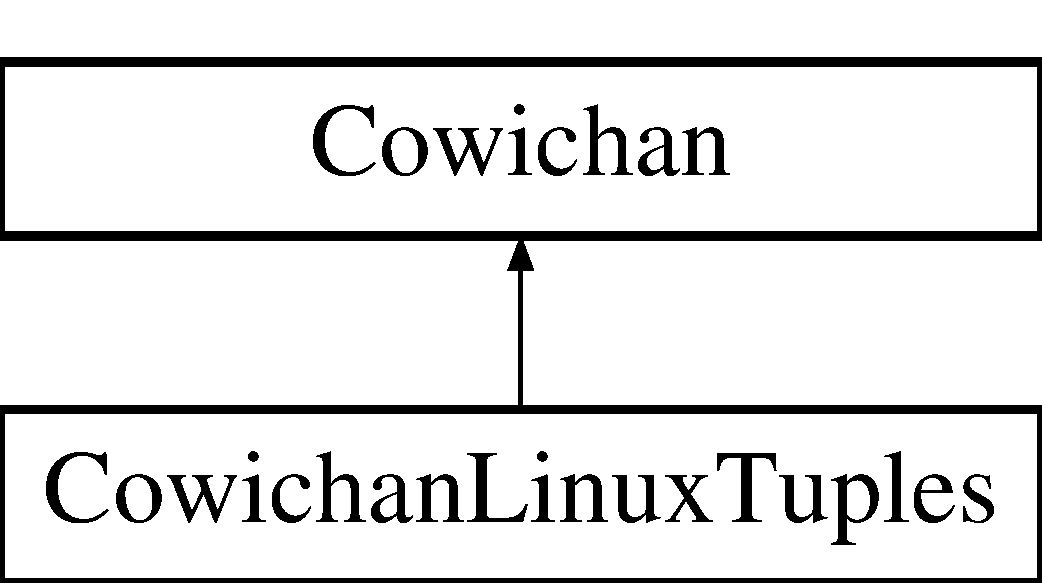
\includegraphics[height=2cm]{class_cowichan_linux_tuples}
\end{center}
\end{figure}
\subsection*{Static Public Attributes}
\begin{CompactItemize}
\item 
static const char $\ast$ \hyperlink{class_cowichan_linux_tuples_606850f3470fa6dabc5073f30f3cbdff}{SERVER} = \char`\"{}localhost\char`\"{}
\item 
static const int \hyperlink{class_cowichan_linux_tuples_8147ab1e9ceb24271c0f8d05b7b050d5}{PORT} = 25000
\item 
static const int \hyperlink{class_cowichan_linux_tuples_a6a295eddcf047ef4199a1f60c29f9ee}{NUM\_\-WORKERS} = 2
\end{CompactItemize}
\subsection*{Protected Member Functions}
\begin{CompactItemize}
\item 
void \hyperlink{class_cowichan_linux_tuples_8774404842868381379ec627e8373cec}{mandel} (\hyperlink{cowichan_8hpp_82321152ddeeefe9c61350a42ed9e7af}{IntMatrix} matrix)
\item 
void \hyperlink{class_cowichan_linux_tuples_ff90c6a27db51366570b70d352de7fab}{randmat} (\hyperlink{cowichan_8hpp_82321152ddeeefe9c61350a42ed9e7af}{IntMatrix} matrix)
\item 
void \hyperlink{class_cowichan_linux_tuples_f3bd58ad2653f06d242d473e7bffda0b}{half} (\hyperlink{cowichan_8hpp_82321152ddeeefe9c61350a42ed9e7af}{IntMatrix} matrixIn, \hyperlink{cowichan_8hpp_82321152ddeeefe9c61350a42ed9e7af}{IntMatrix} matrixOut)
\item 
void \hyperlink{class_cowichan_linux_tuples_5497a17a63cc5faad7afa54d013ea741}{invperc} (\hyperlink{cowichan_8hpp_82321152ddeeefe9c61350a42ed9e7af}{IntMatrix} matrix, \hyperlink{cowichan_8hpp_a64c8df2f1e9c8ea68a7bcc19aca683e}{BoolMatrix} mask)
\item 
void \hyperlink{class_cowichan_linux_tuples_b8cf055ec3d42a1ccde6d818c5a43a74}{thresh} (\hyperlink{cowichan_8hpp_82321152ddeeefe9c61350a42ed9e7af}{IntMatrix} matrix, \hyperlink{cowichan_8hpp_a64c8df2f1e9c8ea68a7bcc19aca683e}{BoolMatrix} mask)
\item 
void \hyperlink{class_cowichan_linux_tuples_967138bbdead76eec50f31465dd9d5f1}{life} (\hyperlink{cowichan_8hpp_a64c8df2f1e9c8ea68a7bcc19aca683e}{BoolMatrix} matrixIn, \hyperlink{cowichan_8hpp_a64c8df2f1e9c8ea68a7bcc19aca683e}{BoolMatrix} matrixOut)
\item 
void \hyperlink{class_cowichan_linux_tuples_2b1a77ecbd01ec847cf63fe7ebb50e35}{winnow} (\hyperlink{cowichan_8hpp_82321152ddeeefe9c61350a42ed9e7af}{IntMatrix} matrix, \hyperlink{cowichan_8hpp_a64c8df2f1e9c8ea68a7bcc19aca683e}{BoolMatrix} mask, \hyperlink{class_point}{PointVector} points)
\item 
void \hyperlink{class_cowichan_linux_tuples_922209c219bb5b9268263dae4000ea81}{norm} (\hyperlink{class_point}{PointVector} pointsIn, \hyperlink{class_point}{PointVector} pointsOut)
\item 
void \hyperlink{class_cowichan_linux_tuples_501f87594d62af261ff0b1954a60ddc4}{hull} (\hyperlink{class_point}{PointVector} pointsIn, \hyperlink{class_point}{PointVector} pointsOut)
\item 
void \hyperlink{class_cowichan_linux_tuples_b16e1c3b60f920c12460a74289558dcb}{outer} (\hyperlink{class_point}{PointVector} points, \hyperlink{cowichan_8hpp_3fb46f939e55c239fbc95656fc0f3399}{Matrix} matrix, \hyperlink{cowichan_8hpp_02bc1553e241b9b33408482658b3c355}{Vector} vector)
\item 
void \hyperlink{class_cowichan_linux_tuples_fd3e659afb38415f56fd508333b7bb1b}{gauss} (\hyperlink{cowichan_8hpp_3fb46f939e55c239fbc95656fc0f3399}{Matrix} matrix, \hyperlink{cowichan_8hpp_02bc1553e241b9b33408482658b3c355}{Vector} target, \hyperlink{cowichan_8hpp_02bc1553e241b9b33408482658b3c355}{Vector} solution)
\item 
void \hyperlink{class_cowichan_linux_tuples_aa2c469c3f520a5a56c5ec1ac9a5a6c6}{sor} (\hyperlink{cowichan_8hpp_3fb46f939e55c239fbc95656fc0f3399}{Matrix} matrix, \hyperlink{cowichan_8hpp_02bc1553e241b9b33408482658b3c355}{Vector} target, \hyperlink{cowichan_8hpp_02bc1553e241b9b33408482658b3c355}{Vector} solution)
\item 
void \hyperlink{class_cowichan_linux_tuples_c4874f09c54056ac94d00f9e341a94f4}{product} (\hyperlink{cowichan_8hpp_3fb46f939e55c239fbc95656fc0f3399}{Matrix} matrix, \hyperlink{cowichan_8hpp_02bc1553e241b9b33408482658b3c355}{Vector} candidate, \hyperlink{cowichan_8hpp_02bc1553e241b9b33408482658b3c355}{Vector} solution)
\item 
\hyperlink{cowichan_8hpp_4d521b2c54a1f6312cc8fa04827eaf98}{real} \hyperlink{class_cowichan_linux_tuples_213185666ea7dd0c9abc59899b454086}{vecdiff} (\hyperlink{cowichan_8hpp_02bc1553e241b9b33408482658b3c355}{Vector} actual, \hyperlink{cowichan_8hpp_02bc1553e241b9b33408482658b3c355}{Vector} computed)
\item 
void \hyperlink{class_cowichan_linux_tuples_fd49b2a0af64bafb93a5fe1210c68acd}{chain} (bool use\_\-randmat, bool use\_\-thresh)
\end{CompactItemize}


\subsection{Detailed Description}
The LinuxTuples implementation of the \hyperlink{class_cowichan}{Cowichan} problem set. 

\subsection{Member Function Documentation}
\hypertarget{class_cowichan_linux_tuples_fd49b2a0af64bafb93a5fe1210c68acd}{
\index{CowichanLinuxTuples@{CowichanLinuxTuples}!chain@{chain}}
\index{chain@{chain}!CowichanLinuxTuples@{CowichanLinuxTuples}}
\subsubsection[{chain}]{\setlength{\rightskip}{0pt plus 5cm}void CowichanLinuxTuples::chain (bool {\em use\_\-randmat}, \/  bool {\em use\_\-thresh})\hspace{0.3cm}{\tt  \mbox{[}protected\mbox{]}}}}
\label{class_cowichan_linux_tuples_fd49b2a0af64bafb93a5fe1210c68acd}


Runs the cowichan problem set, chained together. \begin{Desc}
\item[Parameters:]
\begin{description}
\item[{\em use\_\-randmat}]true: generate a random matrix. false: use a window of the mandelbrot set. \item[{\em use\_\-thresh}]true: use image thresholding for int-$>$bool. false: use invasion percolation for int-$>$bool. \end{description}
\end{Desc}


Reimplemented from \hyperlink{class_cowichan_08ee88eb612571e8faa20b2645dc906d}{Cowichan}.\hypertarget{class_cowichan_linux_tuples_fd3e659afb38415f56fd508333b7bb1b}{
\index{CowichanLinuxTuples@{CowichanLinuxTuples}!gauss@{gauss}}
\index{gauss@{gauss}!CowichanLinuxTuples@{CowichanLinuxTuples}}
\subsubsection[{gauss}]{\setlength{\rightskip}{0pt plus 5cm}void CowichanLinuxTuples::gauss ({\bf Matrix} {\em matrix}, \/  {\bf Vector} {\em target}, \/  {\bf Vector} {\em solution})\hspace{0.3cm}{\tt  \mbox{[}protected, virtual\mbox{]}}}}
\label{class_cowichan_linux_tuples_fd3e659afb38415f56fd508333b7bb1b}


For description see \hyperlink{index_gauss_sec}{11. Gaussian Elimination} \begin{Desc}
\item[Parameters:]
\begin{description}
\item[{\em matrix}]matrix A in AX = V. \item[{\em target}]vector V in AX = V. \item[{\em solution}]vector X in AX = V. \end{description}
\end{Desc}


Implements \hyperlink{class_cowichan_aa9aac74b96dc5ed33e821d94649d1b2}{Cowichan}.\hypertarget{class_cowichan_linux_tuples_f3bd58ad2653f06d242d473e7bffda0b}{
\index{CowichanLinuxTuples@{CowichanLinuxTuples}!half@{half}}
\index{half@{half}!CowichanLinuxTuples@{CowichanLinuxTuples}}
\subsubsection[{half}]{\setlength{\rightskip}{0pt plus 5cm}void CowichanLinuxTuples::half ({\bf IntMatrix} {\em matrixIn}, \/  {\bf IntMatrix} {\em matrixOut})\hspace{0.3cm}{\tt  \mbox{[}protected, virtual\mbox{]}}}}
\label{class_cowichan_linux_tuples_f3bd58ad2653f06d242d473e7bffda0b}


For description see \hyperlink{index_half_sec}{3. Two-Dimensional Shuffle} \begin{Desc}
\item[Parameters:]
\begin{description}
\item[{\em matrixIn}]matrix to shuffle. \item[{\em matrixOut}]shuffled matrix. \end{description}
\end{Desc}


Implements \hyperlink{class_cowichan_308603053675bccbe631f04af921f57c}{Cowichan}.\hypertarget{class_cowichan_linux_tuples_501f87594d62af261ff0b1954a60ddc4}{
\index{CowichanLinuxTuples@{CowichanLinuxTuples}!hull@{hull}}
\index{hull@{hull}!CowichanLinuxTuples@{CowichanLinuxTuples}}
\subsubsection[{hull}]{\setlength{\rightskip}{0pt plus 5cm}void CowichanLinuxTuples::hull ({\bf PointVector} {\em pointsIn}, \/  {\bf PointVector} {\em pointsOut})\hspace{0.3cm}{\tt  \mbox{[}protected, virtual\mbox{]}}}}
\label{class_cowichan_linux_tuples_501f87594d62af261ff0b1954a60ddc4}


For description see \hyperlink{index_hull_sec}{9. Convex Hull} \begin{Desc}
\item[Parameters:]
\begin{description}
\item[{\em pointsIn}]points to run convex hull on. \item[{\em pointsOut}]reordered points from pointsIn. \end{description}
\end{Desc}


Implements \hyperlink{class_cowichan_0c6b68ae3c059b66893405f8530a2e0a}{Cowichan}.\hypertarget{class_cowichan_linux_tuples_5497a17a63cc5faad7afa54d013ea741}{
\index{CowichanLinuxTuples@{CowichanLinuxTuples}!invperc@{invperc}}
\index{invperc@{invperc}!CowichanLinuxTuples@{CowichanLinuxTuples}}
\subsubsection[{invperc}]{\setlength{\rightskip}{0pt plus 5cm}void CowichanLinuxTuples::invperc ({\bf IntMatrix} {\em matrix}, \/  {\bf BoolMatrix} {\em mask})\hspace{0.3cm}{\tt  \mbox{[}protected, virtual\mbox{]}}}}
\label{class_cowichan_linux_tuples_5497a17a63cc5faad7afa54d013ea741}


For description see \hyperlink{index_invperc_sec}{4. Invasion Percolation} \begin{Desc}
\item[Parameters:]
\begin{description}
\item[{\em matrix}]filling resistance matrix. \item[{\em mask}]filled cells. \end{description}
\end{Desc}


Implements \hyperlink{class_cowichan_ea126792a31e54a8722663b7ea768955}{Cowichan}.\hypertarget{class_cowichan_linux_tuples_967138bbdead76eec50f31465dd9d5f1}{
\index{CowichanLinuxTuples@{CowichanLinuxTuples}!life@{life}}
\index{life@{life}!CowichanLinuxTuples@{CowichanLinuxTuples}}
\subsubsection[{life}]{\setlength{\rightskip}{0pt plus 5cm}void CowichanLinuxTuples::life ({\bf BoolMatrix} {\em matrixIn}, \/  {\bf BoolMatrix} {\em matrixOut})\hspace{0.3cm}{\tt  \mbox{[}protected, virtual\mbox{]}}}}
\label{class_cowichan_linux_tuples_967138bbdead76eec50f31465dd9d5f1}


For description see \hyperlink{index_life_sec}{6. Game of Life} \begin{Desc}
\item[Parameters:]
\begin{description}
\item[{\em matrixIn}]initial world. \item[{\em matrixOut}]final world. \end{description}
\end{Desc}


Implements \hyperlink{class_cowichan_d449595ef2fe934bdd128ac8b1f51d07}{Cowichan}.\hypertarget{class_cowichan_linux_tuples_8774404842868381379ec627e8373cec}{
\index{CowichanLinuxTuples@{CowichanLinuxTuples}!mandel@{mandel}}
\index{mandel@{mandel}!CowichanLinuxTuples@{CowichanLinuxTuples}}
\subsubsection[{mandel}]{\setlength{\rightskip}{0pt plus 5cm}void CowichanLinuxTuples::mandel ({\bf IntMatrix} {\em matrix})\hspace{0.3cm}{\tt  \mbox{[}protected, virtual\mbox{]}}}}
\label{class_cowichan_linux_tuples_8774404842868381379ec627e8373cec}


For description see \hyperlink{index_mandel_sec}{1. Mandelbrot Set Generation} \begin{Desc}
\item[Parameters:]
\begin{description}
\item[{\em matrix}]matrix to fill. \end{description}
\end{Desc}


Implements \hyperlink{class_cowichan_ec6cc4eb2ad444474b923532167e98a2}{Cowichan}.\hypertarget{class_cowichan_linux_tuples_922209c219bb5b9268263dae4000ea81}{
\index{CowichanLinuxTuples@{CowichanLinuxTuples}!norm@{norm}}
\index{norm@{norm}!CowichanLinuxTuples@{CowichanLinuxTuples}}
\subsubsection[{norm}]{\setlength{\rightskip}{0pt plus 5cm}void CowichanLinuxTuples::norm ({\bf PointVector} {\em pointsIn}, \/  {\bf PointVector} {\em pointsOut})\hspace{0.3cm}{\tt  \mbox{[}protected, virtual\mbox{]}}}}
\label{class_cowichan_linux_tuples_922209c219bb5b9268263dae4000ea81}


For description see \hyperlink{index_norm_sec}{8. Point Location Normalization} \begin{Desc}
\item[Parameters:]
\begin{description}
\item[{\em pointsIn}]points to normalize. \item[{\em pointsOut}]normalized points. \end{description}
\end{Desc}


Implements \hyperlink{class_cowichan_3df21e3c627958114e045c3559a29f30}{Cowichan}.\hypertarget{class_cowichan_linux_tuples_b16e1c3b60f920c12460a74289558dcb}{
\index{CowichanLinuxTuples@{CowichanLinuxTuples}!outer@{outer}}
\index{outer@{outer}!CowichanLinuxTuples@{CowichanLinuxTuples}}
\subsubsection[{outer}]{\setlength{\rightskip}{0pt plus 5cm}void CowichanLinuxTuples::outer ({\bf PointVector} {\em points}, \/  {\bf Matrix} {\em matrix}, \/  {\bf Vector} {\em vector})\hspace{0.3cm}{\tt  \mbox{[}protected, virtual\mbox{]}}}}
\label{class_cowichan_linux_tuples_b16e1c3b60f920c12460a74289558dcb}


For description see \hyperlink{index_outer_sec}{10. Outer Product} \begin{Desc}
\item[Parameters:]
\begin{description}
\item[{\em points}]vector of points. \item[{\em matrix}]resulting distance matrix. \item[{\em vector}]resulting distance vector. \end{description}
\end{Desc}


Implements \hyperlink{class_cowichan_52f17221019290b88334b0ca7f3bcdb9}{Cowichan}.\hypertarget{class_cowichan_linux_tuples_c4874f09c54056ac94d00f9e341a94f4}{
\index{CowichanLinuxTuples@{CowichanLinuxTuples}!product@{product}}
\index{product@{product}!CowichanLinuxTuples@{CowichanLinuxTuples}}
\subsubsection[{product}]{\setlength{\rightskip}{0pt plus 5cm}void CowichanLinuxTuples::product ({\bf Matrix} {\em matrix}, \/  {\bf Vector} {\em candidate}, \/  {\bf Vector} {\em solution})\hspace{0.3cm}{\tt  \mbox{[}protected, virtual\mbox{]}}}}
\label{class_cowichan_linux_tuples_c4874f09c54056ac94d00f9e341a94f4}


For description see \hyperlink{index_product_sec}{13. Matrix-Vector Product} \begin{Desc}
\item[Parameters:]
\begin{description}
\item[{\em matrix}]matrix A in AX = V. \item[{\em candidate}]vector X in AX = V. \item[{\em solution}]vector V in AX = V. \end{description}
\end{Desc}


Implements \hyperlink{class_cowichan_3d7d4b581a1d6f0392dc452830fb3b03}{Cowichan}.\hypertarget{class_cowichan_linux_tuples_ff90c6a27db51366570b70d352de7fab}{
\index{CowichanLinuxTuples@{CowichanLinuxTuples}!randmat@{randmat}}
\index{randmat@{randmat}!CowichanLinuxTuples@{CowichanLinuxTuples}}
\subsubsection[{randmat}]{\setlength{\rightskip}{0pt plus 5cm}void CowichanLinuxTuples::randmat ({\bf IntMatrix} {\em matrix})\hspace{0.3cm}{\tt  \mbox{[}protected, virtual\mbox{]}}}}
\label{class_cowichan_linux_tuples_ff90c6a27db51366570b70d352de7fab}


For description see \hyperlink{index_randmat_sec}{2. Random Number Generation} \begin{Desc}
\item[Parameters:]
\begin{description}
\item[{\em matrix}]matrix to fill. \end{description}
\end{Desc}


Implements \hyperlink{class_cowichan_c44cacf9d9e363a5b076bcee8b9a7a73}{Cowichan}.\hypertarget{class_cowichan_linux_tuples_aa2c469c3f520a5a56c5ec1ac9a5a6c6}{
\index{CowichanLinuxTuples@{CowichanLinuxTuples}!sor@{sor}}
\index{sor@{sor}!CowichanLinuxTuples@{CowichanLinuxTuples}}
\subsubsection[{sor}]{\setlength{\rightskip}{0pt plus 5cm}void CowichanLinuxTuples::sor ({\bf Matrix} {\em matrix}, \/  {\bf Vector} {\em target}, \/  {\bf Vector} {\em solution})\hspace{0.3cm}{\tt  \mbox{[}protected, virtual\mbox{]}}}}
\label{class_cowichan_linux_tuples_aa2c469c3f520a5a56c5ec1ac9a5a6c6}


For description see \hyperlink{index_sor_sec}{12. Successive Over-Relaxation} \begin{Desc}
\item[Parameters:]
\begin{description}
\item[{\em matrix}]matrix A in AX = V. \item[{\em target}]vector V in AX = V. \item[{\em solution}]vector X in AX = V. \end{description}
\end{Desc}


Implements \hyperlink{class_cowichan_92d8d9ae77208115fdfe69e1174f601c}{Cowichan}.\hypertarget{class_cowichan_linux_tuples_b8cf055ec3d42a1ccde6d818c5a43a74}{
\index{CowichanLinuxTuples@{CowichanLinuxTuples}!thresh@{thresh}}
\index{thresh@{thresh}!CowichanLinuxTuples@{CowichanLinuxTuples}}
\subsubsection[{thresh}]{\setlength{\rightskip}{0pt plus 5cm}void CowichanLinuxTuples::thresh ({\bf IntMatrix} {\em matrix}, \/  {\bf BoolMatrix} {\em mask})\hspace{0.3cm}{\tt  \mbox{[}protected, virtual\mbox{]}}}}
\label{class_cowichan_linux_tuples_b8cf055ec3d42a1ccde6d818c5a43a74}


For description see \hyperlink{index_thresh_sec}{5. Histogram Thresholding} \begin{Desc}
\item[Parameters:]
\begin{description}
\item[{\em matrix}]image. \item[{\em mask}]image after thresholding. \end{description}
\end{Desc}


Implements \hyperlink{class_cowichan_a0b633b8c1f21884e0998a9c7020c08c}{Cowichan}.\hypertarget{class_cowichan_linux_tuples_213185666ea7dd0c9abc59899b454086}{
\index{CowichanLinuxTuples@{CowichanLinuxTuples}!vecdiff@{vecdiff}}
\index{vecdiff@{vecdiff}!CowichanLinuxTuples@{CowichanLinuxTuples}}
\subsubsection[{vecdiff}]{\setlength{\rightskip}{0pt plus 5cm}{\bf real} CowichanLinuxTuples::vecdiff ({\bf Vector} {\em actual}, \/  {\bf Vector} {\em computed})\hspace{0.3cm}{\tt  \mbox{[}protected, virtual\mbox{]}}}}
\label{class_cowichan_linux_tuples_213185666ea7dd0c9abc59899b454086}


For description see \hyperlink{index_vecdiff_sec}{14. 1-Norm Vector Difference} \begin{Desc}
\item[Parameters:]
\begin{description}
\item[{\em actual}]first vector. \item[{\em computed}]second vector. \end{description}
\end{Desc}


Implements \hyperlink{class_cowichan_775d72b5e7d122f9f32555352278250e}{Cowichan}.\hypertarget{class_cowichan_linux_tuples_2b1a77ecbd01ec847cf63fe7ebb50e35}{
\index{CowichanLinuxTuples@{CowichanLinuxTuples}!winnow@{winnow}}
\index{winnow@{winnow}!CowichanLinuxTuples@{CowichanLinuxTuples}}
\subsubsection[{winnow}]{\setlength{\rightskip}{0pt plus 5cm}void CowichanLinuxTuples::winnow ({\bf IntMatrix} {\em matrix}, \/  {\bf BoolMatrix} {\em mask}, \/  {\bf PointVector} {\em points})\hspace{0.3cm}{\tt  \mbox{[}protected, virtual\mbox{]}}}}
\label{class_cowichan_linux_tuples_2b1a77ecbd01ec847cf63fe7ebb50e35}


For description see \hyperlink{index_winnow_sec}{7. Weighted Point Selection} \begin{Desc}
\item[Parameters:]
\begin{description}
\item[{\em matrix}]integer matrix. \item[{\em mask}]boolean matrix. \item[{\em points}]evenly selected points. \end{description}
\end{Desc}


Implements \hyperlink{class_cowichan_13d60e06ced3b5da79d62c133ce82337}{Cowichan}.

\subsection{Member Data Documentation}
\hypertarget{class_cowichan_linux_tuples_a6a295eddcf047ef4199a1f60c29f9ee}{
\index{CowichanLinuxTuples@{CowichanLinuxTuples}!NUM\_\-WORKERS@{NUM\_\-WORKERS}}
\index{NUM\_\-WORKERS@{NUM\_\-WORKERS}!CowichanLinuxTuples@{CowichanLinuxTuples}}
\subsubsection[{NUM\_\-WORKERS}]{\setlength{\rightskip}{0pt plus 5cm}const int {\bf CowichanLinuxTuples::NUM\_\-WORKERS} = 2\hspace{0.3cm}{\tt  \mbox{[}static\mbox{]}}}}
\label{class_cowichan_linux_tuples_a6a295eddcf047ef4199a1f60c29f9ee}


The number of worker processes to spawn. \hypertarget{class_cowichan_linux_tuples_8147ab1e9ceb24271c0f8d05b7b050d5}{
\index{CowichanLinuxTuples@{CowichanLinuxTuples}!PORT@{PORT}}
\index{PORT@{PORT}!CowichanLinuxTuples@{CowichanLinuxTuples}}
\subsubsection[{PORT}]{\setlength{\rightskip}{0pt plus 5cm}const int {\bf CowichanLinuxTuples::PORT} = 25000\hspace{0.3cm}{\tt  \mbox{[}static\mbox{]}}}}
\label{class_cowichan_linux_tuples_8147ab1e9ceb24271c0f8d05b7b050d5}


The port number the LinuxTuples server is running on. \hypertarget{class_cowichan_linux_tuples_606850f3470fa6dabc5073f30f3cbdff}{
\index{CowichanLinuxTuples@{CowichanLinuxTuples}!SERVER@{SERVER}}
\index{SERVER@{SERVER}!CowichanLinuxTuples@{CowichanLinuxTuples}}
\subsubsection[{SERVER}]{\setlength{\rightskip}{0pt plus 5cm}const char $\ast$ {\bf CowichanLinuxTuples::SERVER} = \char`\"{}localhost\char`\"{}\hspace{0.3cm}{\tt  \mbox{[}static\mbox{]}}}}
\label{class_cowichan_linux_tuples_606850f3470fa6dabc5073f30f3cbdff}


The host where the LinuxTuples server can be found. 

The documentation for this class was generated from the following files:\begin{CompactItemize}
\item 
cowichan\_\-lt/src/\hyperlink{cowichan__lt_8hpp}{cowichan\_\-lt.hpp}\item 
cowichan\_\-lt/src/\hyperlink{cowichan__lt_8cpp}{cowichan\_\-lt.cpp}\item 
cowichan\_\-lt/src/\hyperlink{cowichan__lt_2src_2gauss_8cpp}{gauss.cpp}\item 
cowichan\_\-lt/src/\hyperlink{cowichan__lt_2src_2half_8cpp}{half.cpp}\item 
cowichan\_\-lt/src/\hyperlink{cowichan__lt_2src_2hull_8cpp}{hull.cpp}\item 
cowichan\_\-lt/src/\hyperlink{cowichan__lt_2src_2invperc_8cpp}{invperc.cpp}\item 
cowichan\_\-lt/src/\hyperlink{cowichan__lt_2src_2life_8cpp}{life.cpp}\item 
cowichan\_\-lt/src/\hyperlink{cowichan__lt_2src_2mandel_8cpp}{mandel.cpp}\item 
cowichan\_\-lt/src/\hyperlink{cowichan__lt_2src_2norm_8cpp}{norm.cpp}\item 
cowichan\_\-lt/src/\hyperlink{cowichan__lt_2src_2outer_8cpp}{outer.cpp}\item 
cowichan\_\-lt/src/\hyperlink{cowichan__lt_2src_2product_8cpp}{product.cpp}\item 
cowichan\_\-lt/src/\hyperlink{cowichan__lt_2src_2randmat_8cpp}{randmat.cpp}\item 
cowichan\_\-lt/src/\hyperlink{cowichan__lt_2src_2sor_8cpp}{sor.cpp}\item 
cowichan\_\-lt/src/\hyperlink{cowichan__lt_2src_2thresh_8cpp}{thresh.cpp}\item 
cowichan\_\-lt/src/\hyperlink{cowichan__lt_2src_2vecdiff_8cpp}{vecdiff.cpp}\item 
cowichan\_\-lt/src/\hyperlink{cowichan__lt_2src_2winnow_8cpp}{winnow.cpp}\end{CompactItemize}

\hypertarget{class_cowichan_m_p_i}{
\section{CowichanMPI Class Reference}
\label{class_cowichan_m_p_i}\index{CowichanMPI@{CowichanMPI}}
}
Boost Message Passing Interface (MPI) implementation.  


{\tt \#include $<$cowichan\_\-mpi.hpp$>$}

Inheritance diagram for CowichanMPI::\begin{figure}[H]
\begin{center}
\leavevmode
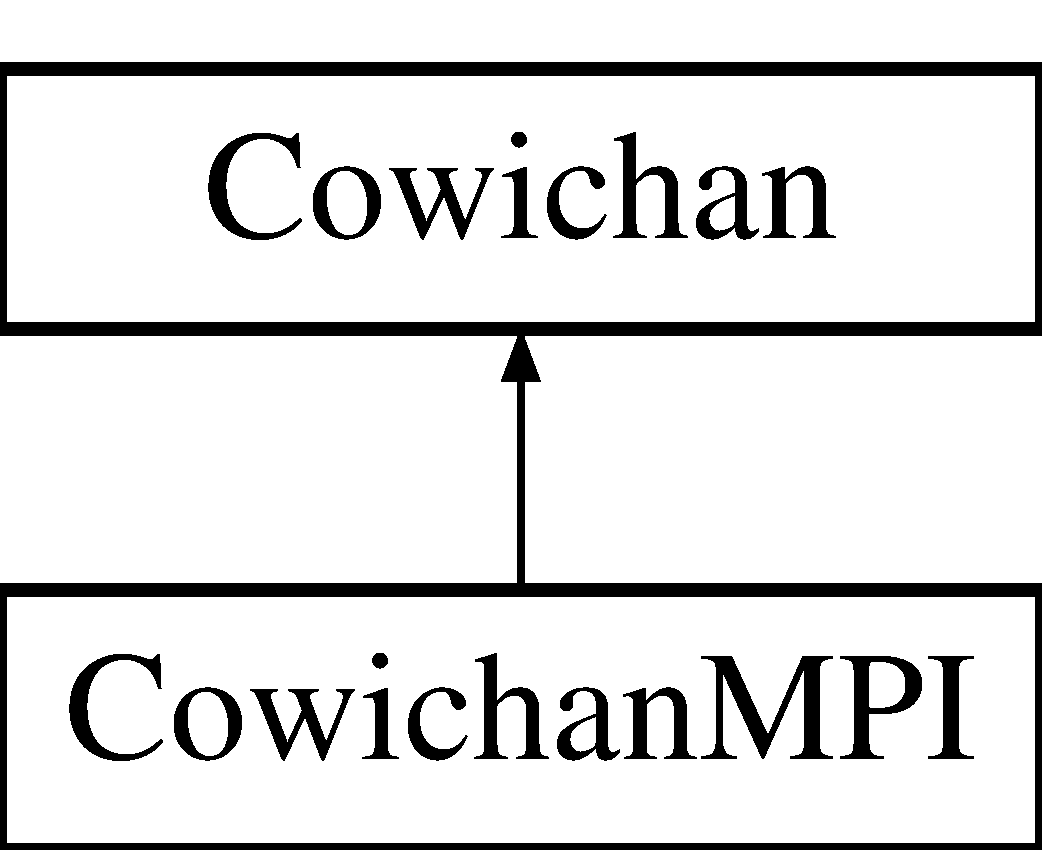
\includegraphics[height=2cm]{class_cowichan_m_p_i}
\end{center}
\end{figure}
\subsection*{Public Member Functions}
\begin{CompactItemize}
\item 
\hyperlink{class_cowichan_m_p_i_ba4175b1aadbab75285b47819477dedf}{CowichanMPI} (const mpi::communicator \&\hyperlink{class_cowichan_m_p_i_cf8ae701dfbb7c17dcec165800c16969}{world})
\end{CompactItemize}
\subsection*{Public Attributes}
\begin{CompactItemize}
\item 
const mpi::communicator \& \hyperlink{class_cowichan_m_p_i_cf8ae701dfbb7c17dcec165800c16969}{world}
\end{CompactItemize}
\subsection*{Protected Member Functions}
\begin{CompactItemize}
\item 
void \hyperlink{class_cowichan_m_p_i_58274fc55ed8a352a8924b130f3b5d2e}{mandel} (\hyperlink{cowichan_8hpp_82321152ddeeefe9c61350a42ed9e7af}{IntMatrix} matrix)
\item 
void \hyperlink{class_cowichan_m_p_i_6805f21144aeaeddc4549e1b2b42bca8}{randmat} (\hyperlink{cowichan_8hpp_82321152ddeeefe9c61350a42ed9e7af}{IntMatrix} matrix)
\item 
void \hyperlink{class_cowichan_m_p_i_154bbd1a400ee4571f761bff1cdf67cd}{half} (\hyperlink{cowichan_8hpp_82321152ddeeefe9c61350a42ed9e7af}{IntMatrix} matrixIn, \hyperlink{cowichan_8hpp_82321152ddeeefe9c61350a42ed9e7af}{IntMatrix} matrixOut)
\item 
void \hyperlink{class_cowichan_m_p_i_bcd0f18fcccc8973ddaacf4dda190b53}{invperc} (\hyperlink{cowichan_8hpp_82321152ddeeefe9c61350a42ed9e7af}{IntMatrix} matrix, \hyperlink{cowichan_8hpp_a64c8df2f1e9c8ea68a7bcc19aca683e}{BoolMatrix} mask)
\item 
void \hyperlink{class_cowichan_m_p_i_49ff96b091a61e9cfd9aad8824e7fbbd}{thresh} (\hyperlink{cowichan_8hpp_82321152ddeeefe9c61350a42ed9e7af}{IntMatrix} matrix, \hyperlink{cowichan_8hpp_a64c8df2f1e9c8ea68a7bcc19aca683e}{BoolMatrix} mask)
\item 
void \hyperlink{class_cowichan_m_p_i_9c739951d036ef7905bda7cb896e0edf}{life} (\hyperlink{cowichan_8hpp_a64c8df2f1e9c8ea68a7bcc19aca683e}{BoolMatrix} matrixIn, \hyperlink{cowichan_8hpp_a64c8df2f1e9c8ea68a7bcc19aca683e}{BoolMatrix} matrixOut)
\item 
void \hyperlink{class_cowichan_m_p_i_9be48d86fc51ce13ef79d5fe2c8a16e0}{winnow} (\hyperlink{cowichan_8hpp_82321152ddeeefe9c61350a42ed9e7af}{IntMatrix} matrix, \hyperlink{cowichan_8hpp_a64c8df2f1e9c8ea68a7bcc19aca683e}{BoolMatrix} mask, \hyperlink{class_point}{PointVector} points)
\item 
void \hyperlink{class_cowichan_m_p_i_11df49e804427d4a0d085f4cff9302d0}{norm} (\hyperlink{class_point}{PointVector} pointsIn, \hyperlink{class_point}{PointVector} pointsOut)
\item 
void \hyperlink{class_cowichan_m_p_i_22b3dce35fd93635bd4c1596e7fb839c}{hull} (\hyperlink{class_point}{PointVector} pointsIn, \hyperlink{class_point}{PointVector} pointsOut)
\item 
void \hyperlink{class_cowichan_m_p_i_39fcc8a331b0e26438fbf43fa01cf7c1}{outer} (\hyperlink{class_point}{PointVector} points, \hyperlink{cowichan_8hpp_3fb46f939e55c239fbc95656fc0f3399}{Matrix} matrix, \hyperlink{cowichan_8hpp_02bc1553e241b9b33408482658b3c355}{Vector} vector)
\item 
void \hyperlink{class_cowichan_m_p_i_975f8da6c166fe1db3cf9341eeaab000}{gauss} (\hyperlink{cowichan_8hpp_3fb46f939e55c239fbc95656fc0f3399}{Matrix} matrix, \hyperlink{cowichan_8hpp_02bc1553e241b9b33408482658b3c355}{Vector} target, \hyperlink{cowichan_8hpp_02bc1553e241b9b33408482658b3c355}{Vector} solution)
\item 
void \hyperlink{class_cowichan_m_p_i_7388c844e8aa73ab0923443a3a7ef069}{sor} (\hyperlink{cowichan_8hpp_3fb46f939e55c239fbc95656fc0f3399}{Matrix} matrix, \hyperlink{cowichan_8hpp_02bc1553e241b9b33408482658b3c355}{Vector} target, \hyperlink{cowichan_8hpp_02bc1553e241b9b33408482658b3c355}{Vector} solution)
\item 
void \hyperlink{class_cowichan_m_p_i_1b7dccf774caccb26839cd29fe0a5cb0}{product} (\hyperlink{cowichan_8hpp_3fb46f939e55c239fbc95656fc0f3399}{Matrix} matrix, \hyperlink{cowichan_8hpp_02bc1553e241b9b33408482658b3c355}{Vector} candidate, \hyperlink{cowichan_8hpp_02bc1553e241b9b33408482658b3c355}{Vector} solution)
\item 
\hyperlink{cowichan_8hpp_4d521b2c54a1f6312cc8fa04827eaf98}{real} \hyperlink{class_cowichan_m_p_i_c5470a2876efecf843b19c37c21ecf19}{vecdiff} (\hyperlink{cowichan_8hpp_02bc1553e241b9b33408482658b3c355}{Vector} actual, \hyperlink{cowichan_8hpp_02bc1553e241b9b33408482658b3c355}{Vector} computed)
\end{CompactItemize}


\subsection{Detailed Description}
Boost Message Passing Interface (MPI) implementation. 

Boost MPI is a C++ interface that works with many MPI implementations. For example: MPICH1, MPICH2, OpenMPI.

Tags: distributed memory, message passing, mpi wrapper. 

\subsection{Constructor \& Destructor Documentation}
\hypertarget{class_cowichan_m_p_i_ba4175b1aadbab75285b47819477dedf}{
\index{CowichanMPI@{CowichanMPI}!CowichanMPI@{CowichanMPI}}
\index{CowichanMPI@{CowichanMPI}!CowichanMPI@{CowichanMPI}}
\subsubsection[{CowichanMPI}]{\setlength{\rightskip}{0pt plus 5cm}CowichanMPI::CowichanMPI (const mpi::communicator \& {\em world})}}
\label{class_cowichan_m_p_i_ba4175b1aadbab75285b47819477dedf}


Constructs a cowichan mpi object. \begin{Desc}
\item[Parameters:]
\begin{description}
\item[{\em world}]global communicator. \end{description}
\end{Desc}


\subsection{Member Function Documentation}
\hypertarget{class_cowichan_m_p_i_975f8da6c166fe1db3cf9341eeaab000}{
\index{CowichanMPI@{CowichanMPI}!gauss@{gauss}}
\index{gauss@{gauss}!CowichanMPI@{CowichanMPI}}
\subsubsection[{gauss}]{\setlength{\rightskip}{0pt plus 5cm}void CowichanMPI::gauss ({\bf Matrix} {\em matrix}, \/  {\bf Vector} {\em target}, \/  {\bf Vector} {\em solution})\hspace{0.3cm}{\tt  \mbox{[}protected, virtual\mbox{]}}}}
\label{class_cowichan_m_p_i_975f8da6c166fe1db3cf9341eeaab000}


For description see \hyperlink{index_gauss_sec}{11. Gaussian Elimination} \begin{Desc}
\item[Parameters:]
\begin{description}
\item[{\em matrix}]matrix A in AX = V. \item[{\em target}]vector V in AX = V. \item[{\em solution}]vector X in AX = V. \end{description}
\end{Desc}


Implements \hyperlink{class_cowichan_aa9aac74b96dc5ed33e821d94649d1b2}{Cowichan}.\hypertarget{class_cowichan_m_p_i_154bbd1a400ee4571f761bff1cdf67cd}{
\index{CowichanMPI@{CowichanMPI}!half@{half}}
\index{half@{half}!CowichanMPI@{CowichanMPI}}
\subsubsection[{half}]{\setlength{\rightskip}{0pt plus 5cm}void CowichanMPI::half ({\bf IntMatrix} {\em matrixIn}, \/  {\bf IntMatrix} {\em matrixOut})\hspace{0.3cm}{\tt  \mbox{[}protected, virtual\mbox{]}}}}
\label{class_cowichan_m_p_i_154bbd1a400ee4571f761bff1cdf67cd}


For description see \hyperlink{index_half_sec}{3. Two-Dimensional Shuffle} \begin{Desc}
\item[Parameters:]
\begin{description}
\item[{\em matrixIn}]matrix to shuffle. \item[{\em matrixOut}]shuffled matrix. \end{description}
\end{Desc}


Implements \hyperlink{class_cowichan_308603053675bccbe631f04af921f57c}{Cowichan}.\hypertarget{class_cowichan_m_p_i_22b3dce35fd93635bd4c1596e7fb839c}{
\index{CowichanMPI@{CowichanMPI}!hull@{hull}}
\index{hull@{hull}!CowichanMPI@{CowichanMPI}}
\subsubsection[{hull}]{\setlength{\rightskip}{0pt plus 5cm}void CowichanMPI::hull ({\bf PointVector} {\em pointsIn}, \/  {\bf PointVector} {\em pointsOut})\hspace{0.3cm}{\tt  \mbox{[}protected, virtual\mbox{]}}}}
\label{class_cowichan_m_p_i_22b3dce35fd93635bd4c1596e7fb839c}


For description see \hyperlink{index_hull_sec}{9. Convex Hull} \begin{Desc}
\item[Parameters:]
\begin{description}
\item[{\em pointsIn}]points to run convex hull on. \item[{\em pointsOut}]reordered points from pointsIn. \end{description}
\end{Desc}


Implements \hyperlink{class_cowichan_0c6b68ae3c059b66893405f8530a2e0a}{Cowichan}.\hypertarget{class_cowichan_m_p_i_bcd0f18fcccc8973ddaacf4dda190b53}{
\index{CowichanMPI@{CowichanMPI}!invperc@{invperc}}
\index{invperc@{invperc}!CowichanMPI@{CowichanMPI}}
\subsubsection[{invperc}]{\setlength{\rightskip}{0pt plus 5cm}void CowichanMPI::invperc ({\bf IntMatrix} {\em matrix}, \/  {\bf BoolMatrix} {\em mask})\hspace{0.3cm}{\tt  \mbox{[}protected, virtual\mbox{]}}}}
\label{class_cowichan_m_p_i_bcd0f18fcccc8973ddaacf4dda190b53}


For description see \hyperlink{index_invperc_sec}{4. Invasion Percolation} \begin{Desc}
\item[Parameters:]
\begin{description}
\item[{\em matrix}]filling resistance matrix. \item[{\em mask}]filled cells. \end{description}
\end{Desc}


Implements \hyperlink{class_cowichan_ea126792a31e54a8722663b7ea768955}{Cowichan}.\hypertarget{class_cowichan_m_p_i_9c739951d036ef7905bda7cb896e0edf}{
\index{CowichanMPI@{CowichanMPI}!life@{life}}
\index{life@{life}!CowichanMPI@{CowichanMPI}}
\subsubsection[{life}]{\setlength{\rightskip}{0pt plus 5cm}void CowichanMPI::life ({\bf BoolMatrix} {\em matrixIn}, \/  {\bf BoolMatrix} {\em matrixOut})\hspace{0.3cm}{\tt  \mbox{[}protected, virtual\mbox{]}}}}
\label{class_cowichan_m_p_i_9c739951d036ef7905bda7cb896e0edf}


For description see \hyperlink{index_life_sec}{6. Game of Life} \begin{Desc}
\item[Parameters:]
\begin{description}
\item[{\em matrixIn}]initial world. \item[{\em matrixOut}]final world. \end{description}
\end{Desc}


Implements \hyperlink{class_cowichan_d449595ef2fe934bdd128ac8b1f51d07}{Cowichan}.\hypertarget{class_cowichan_m_p_i_58274fc55ed8a352a8924b130f3b5d2e}{
\index{CowichanMPI@{CowichanMPI}!mandel@{mandel}}
\index{mandel@{mandel}!CowichanMPI@{CowichanMPI}}
\subsubsection[{mandel}]{\setlength{\rightskip}{0pt plus 5cm}void CowichanMPI::mandel ({\bf IntMatrix} {\em matrix})\hspace{0.3cm}{\tt  \mbox{[}protected, virtual\mbox{]}}}}
\label{class_cowichan_m_p_i_58274fc55ed8a352a8924b130f3b5d2e}


For description see \hyperlink{index_mandel_sec}{1. Mandelbrot Set Generation} \begin{Desc}
\item[Parameters:]
\begin{description}
\item[{\em matrix}]matrix to fill. \end{description}
\end{Desc}


Implements \hyperlink{class_cowichan_ec6cc4eb2ad444474b923532167e98a2}{Cowichan}.\hypertarget{class_cowichan_m_p_i_11df49e804427d4a0d085f4cff9302d0}{
\index{CowichanMPI@{CowichanMPI}!norm@{norm}}
\index{norm@{norm}!CowichanMPI@{CowichanMPI}}
\subsubsection[{norm}]{\setlength{\rightskip}{0pt plus 5cm}void CowichanMPI::norm ({\bf PointVector} {\em pointsIn}, \/  {\bf PointVector} {\em pointsOut})\hspace{0.3cm}{\tt  \mbox{[}protected, virtual\mbox{]}}}}
\label{class_cowichan_m_p_i_11df49e804427d4a0d085f4cff9302d0}


For description see \hyperlink{index_norm_sec}{8. Point Location Normalization} \begin{Desc}
\item[Parameters:]
\begin{description}
\item[{\em pointsIn}]points to normalize. \item[{\em pointsOut}]normalized points. \end{description}
\end{Desc}


Implements \hyperlink{class_cowichan_3df21e3c627958114e045c3559a29f30}{Cowichan}.\hypertarget{class_cowichan_m_p_i_39fcc8a331b0e26438fbf43fa01cf7c1}{
\index{CowichanMPI@{CowichanMPI}!outer@{outer}}
\index{outer@{outer}!CowichanMPI@{CowichanMPI}}
\subsubsection[{outer}]{\setlength{\rightskip}{0pt plus 5cm}void CowichanMPI::outer ({\bf PointVector} {\em points}, \/  {\bf Matrix} {\em matrix}, \/  {\bf Vector} {\em vector})\hspace{0.3cm}{\tt  \mbox{[}protected, virtual\mbox{]}}}}
\label{class_cowichan_m_p_i_39fcc8a331b0e26438fbf43fa01cf7c1}


For description see \hyperlink{index_outer_sec}{10. Outer Product} \begin{Desc}
\item[Parameters:]
\begin{description}
\item[{\em points}]vector of points. \item[{\em matrix}]resulting distance matrix. \item[{\em vector}]resulting distance vector. \end{description}
\end{Desc}


Implements \hyperlink{class_cowichan_52f17221019290b88334b0ca7f3bcdb9}{Cowichan}.\hypertarget{class_cowichan_m_p_i_1b7dccf774caccb26839cd29fe0a5cb0}{
\index{CowichanMPI@{CowichanMPI}!product@{product}}
\index{product@{product}!CowichanMPI@{CowichanMPI}}
\subsubsection[{product}]{\setlength{\rightskip}{0pt plus 5cm}void CowichanMPI::product ({\bf Matrix} {\em matrix}, \/  {\bf Vector} {\em candidate}, \/  {\bf Vector} {\em solution})\hspace{0.3cm}{\tt  \mbox{[}protected, virtual\mbox{]}}}}
\label{class_cowichan_m_p_i_1b7dccf774caccb26839cd29fe0a5cb0}


For description see \hyperlink{index_product_sec}{13. Matrix-Vector Product} \begin{Desc}
\item[Parameters:]
\begin{description}
\item[{\em matrix}]matrix A in AX = V. \item[{\em candidate}]vector X in AX = V. \item[{\em solution}]vector V in AX = V. \end{description}
\end{Desc}


Implements \hyperlink{class_cowichan_3d7d4b581a1d6f0392dc452830fb3b03}{Cowichan}.\hypertarget{class_cowichan_m_p_i_6805f21144aeaeddc4549e1b2b42bca8}{
\index{CowichanMPI@{CowichanMPI}!randmat@{randmat}}
\index{randmat@{randmat}!CowichanMPI@{CowichanMPI}}
\subsubsection[{randmat}]{\setlength{\rightskip}{0pt plus 5cm}void CowichanMPI::randmat ({\bf IntMatrix} {\em matrix})\hspace{0.3cm}{\tt  \mbox{[}protected, virtual\mbox{]}}}}
\label{class_cowichan_m_p_i_6805f21144aeaeddc4549e1b2b42bca8}


For description see \hyperlink{index_randmat_sec}{2. Random Number Generation} \begin{Desc}
\item[Parameters:]
\begin{description}
\item[{\em matrix}]matrix to fill. \end{description}
\end{Desc}


Implements \hyperlink{class_cowichan_c44cacf9d9e363a5b076bcee8b9a7a73}{Cowichan}.\hypertarget{class_cowichan_m_p_i_7388c844e8aa73ab0923443a3a7ef069}{
\index{CowichanMPI@{CowichanMPI}!sor@{sor}}
\index{sor@{sor}!CowichanMPI@{CowichanMPI}}
\subsubsection[{sor}]{\setlength{\rightskip}{0pt plus 5cm}void CowichanMPI::sor ({\bf Matrix} {\em matrix}, \/  {\bf Vector} {\em target}, \/  {\bf Vector} {\em solution})\hspace{0.3cm}{\tt  \mbox{[}protected, virtual\mbox{]}}}}
\label{class_cowichan_m_p_i_7388c844e8aa73ab0923443a3a7ef069}


For description see \hyperlink{index_sor_sec}{12. Successive Over-Relaxation} \begin{Desc}
\item[Parameters:]
\begin{description}
\item[{\em matrix}]matrix A in AX = V. \item[{\em target}]vector V in AX = V. \item[{\em solution}]vector X in AX = V. \end{description}
\end{Desc}


Implements \hyperlink{class_cowichan_92d8d9ae77208115fdfe69e1174f601c}{Cowichan}.\hypertarget{class_cowichan_m_p_i_49ff96b091a61e9cfd9aad8824e7fbbd}{
\index{CowichanMPI@{CowichanMPI}!thresh@{thresh}}
\index{thresh@{thresh}!CowichanMPI@{CowichanMPI}}
\subsubsection[{thresh}]{\setlength{\rightskip}{0pt plus 5cm}void CowichanMPI::thresh ({\bf IntMatrix} {\em matrix}, \/  {\bf BoolMatrix} {\em mask})\hspace{0.3cm}{\tt  \mbox{[}protected, virtual\mbox{]}}}}
\label{class_cowichan_m_p_i_49ff96b091a61e9cfd9aad8824e7fbbd}


For description see \hyperlink{index_thresh_sec}{5. Histogram Thresholding} \begin{Desc}
\item[Parameters:]
\begin{description}
\item[{\em matrix}]image. \item[{\em mask}]image after thresholding. \end{description}
\end{Desc}


Implements \hyperlink{class_cowichan_a0b633b8c1f21884e0998a9c7020c08c}{Cowichan}.\hypertarget{class_cowichan_m_p_i_c5470a2876efecf843b19c37c21ecf19}{
\index{CowichanMPI@{CowichanMPI}!vecdiff@{vecdiff}}
\index{vecdiff@{vecdiff}!CowichanMPI@{CowichanMPI}}
\subsubsection[{vecdiff}]{\setlength{\rightskip}{0pt plus 5cm}{\bf real} CowichanMPI::vecdiff ({\bf Vector} {\em actual}, \/  {\bf Vector} {\em computed})\hspace{0.3cm}{\tt  \mbox{[}protected, virtual\mbox{]}}}}
\label{class_cowichan_m_p_i_c5470a2876efecf843b19c37c21ecf19}


For description see \hyperlink{index_vecdiff_sec}{14. 1-Norm Vector Difference} \begin{Desc}
\item[Parameters:]
\begin{description}
\item[{\em actual}]first vector. \item[{\em computed}]second vector. \end{description}
\end{Desc}


Implements \hyperlink{class_cowichan_775d72b5e7d122f9f32555352278250e}{Cowichan}.\hypertarget{class_cowichan_m_p_i_9be48d86fc51ce13ef79d5fe2c8a16e0}{
\index{CowichanMPI@{CowichanMPI}!winnow@{winnow}}
\index{winnow@{winnow}!CowichanMPI@{CowichanMPI}}
\subsubsection[{winnow}]{\setlength{\rightskip}{0pt plus 5cm}void CowichanMPI::winnow ({\bf IntMatrix} {\em matrix}, \/  {\bf BoolMatrix} {\em mask}, \/  {\bf PointVector} {\em points})\hspace{0.3cm}{\tt  \mbox{[}protected, virtual\mbox{]}}}}
\label{class_cowichan_m_p_i_9be48d86fc51ce13ef79d5fe2c8a16e0}


For description see \hyperlink{index_winnow_sec}{7. Weighted Point Selection} \begin{Desc}
\item[Parameters:]
\begin{description}
\item[{\em matrix}]integer matrix. \item[{\em mask}]boolean matrix. \item[{\em points}]evenly selected points. \end{description}
\end{Desc}


Implements \hyperlink{class_cowichan_13d60e06ced3b5da79d62c133ce82337}{Cowichan}.

\subsection{Member Data Documentation}
\hypertarget{class_cowichan_m_p_i_cf8ae701dfbb7c17dcec165800c16969}{
\index{CowichanMPI@{CowichanMPI}!world@{world}}
\index{world@{world}!CowichanMPI@{CowichanMPI}}
\subsubsection[{world}]{\setlength{\rightskip}{0pt plus 5cm}const mpi::communicator\& {\bf CowichanMPI::world}}}
\label{class_cowichan_m_p_i_cf8ae701dfbb7c17dcec165800c16969}


Global communicator. 

The documentation for this class was generated from the following files:\begin{CompactItemize}
\item 
cowichan\_\-mpi/\hyperlink{cowichan__mpi_8hpp}{cowichan\_\-mpi.hpp}\item 
cowichan\_\-mpi/\hyperlink{cowichan__mpi_8cpp}{cowichan\_\-mpi.cpp}\item 
cowichan\_\-mpi/\hyperlink{cowichan__mpi_2winnow_8cpp}{winnow.cpp}\end{CompactItemize}

\hypertarget{class_cowichan_open_m_p}{
\section{CowichanOpenMP Class Reference}
\label{class_cowichan_open_m_p}\index{CowichanOpenMP@{CowichanOpenMP}}
}
Open Multi-Processing (OpenMP) implementation.  


{\tt \#include $<$cowichan\_\-openmp.hpp$>$}

Inheritance diagram for CowichanOpenMP::\begin{figure}[H]
\begin{center}
\leavevmode
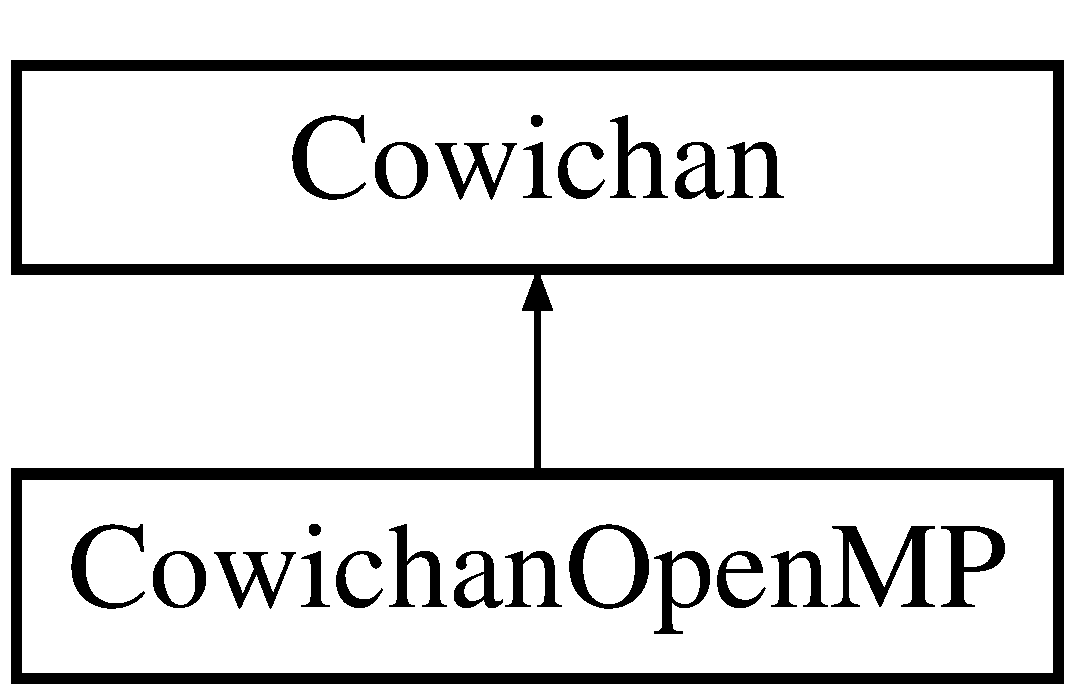
\includegraphics[height=2cm]{class_cowichan_open_m_p}
\end{center}
\end{figure}
\subsection*{Static Public Attributes}
\begin{CompactItemize}
\item 
static const \hyperlink{cowichan_8hpp_5b04577d5d21124855deaad298595371}{index\_\-t} \hyperlink{class_cowichan_open_m_p_52ddfbbead2e1c115806cd07f5630bf5}{HULL\_\-CUTOFF} = 20000
\end{CompactItemize}
\subsection*{Protected Member Functions}
\begin{CompactItemize}
\item 
void \hyperlink{class_cowichan_open_m_p_6809c2738792de047ee59259636c1afd}{mandel} (\hyperlink{cowichan_8hpp_82321152ddeeefe9c61350a42ed9e7af}{IntMatrix} matrix)
\item 
void \hyperlink{class_cowichan_open_m_p_2c7c4e4dd96f82b7280a412c1fceed2c}{randmat} (\hyperlink{cowichan_8hpp_82321152ddeeefe9c61350a42ed9e7af}{IntMatrix} matrix)
\item 
void \hyperlink{class_cowichan_open_m_p_70989ffe182aebf590e39c56e146b0fb}{half} (\hyperlink{cowichan_8hpp_82321152ddeeefe9c61350a42ed9e7af}{IntMatrix} matrixIn, \hyperlink{cowichan_8hpp_82321152ddeeefe9c61350a42ed9e7af}{IntMatrix} matrixOut)
\item 
void \hyperlink{class_cowichan_open_m_p_4824c6b8509b5da835fbc5f64eb3e063}{invperc} (\hyperlink{cowichan_8hpp_82321152ddeeefe9c61350a42ed9e7af}{IntMatrix} matrix, \hyperlink{cowichan_8hpp_a64c8df2f1e9c8ea68a7bcc19aca683e}{BoolMatrix} mask)
\item 
void \hyperlink{class_cowichan_open_m_p_e72c4c0a162f30eac37333bd28db97bc}{thresh} (\hyperlink{cowichan_8hpp_82321152ddeeefe9c61350a42ed9e7af}{IntMatrix} matrix, \hyperlink{cowichan_8hpp_a64c8df2f1e9c8ea68a7bcc19aca683e}{BoolMatrix} mask)
\item 
void \hyperlink{class_cowichan_open_m_p_d24f3ef01289b8f1bd7b864f585daa62}{life} (\hyperlink{cowichan_8hpp_a64c8df2f1e9c8ea68a7bcc19aca683e}{BoolMatrix} matrixIn, \hyperlink{cowichan_8hpp_a64c8df2f1e9c8ea68a7bcc19aca683e}{BoolMatrix} matrixOut)
\item 
void \hyperlink{class_cowichan_open_m_p_4a518f2b5590d4acd670f333471a380a}{winnow} (\hyperlink{cowichan_8hpp_82321152ddeeefe9c61350a42ed9e7af}{IntMatrix} matrix, \hyperlink{cowichan_8hpp_a64c8df2f1e9c8ea68a7bcc19aca683e}{BoolMatrix} mask, \hyperlink{class_point}{PointVector} points)
\item 
void \hyperlink{class_cowichan_open_m_p_4ffbe36816235bc6abec30eae2be2d78}{norm} (\hyperlink{class_point}{PointVector} pointsIn, \hyperlink{class_point}{PointVector} pointsOut)
\item 
void \hyperlink{class_cowichan_open_m_p_cb444dd3e2c0f1f27f4135de0279d09e}{hull} (\hyperlink{class_point}{PointVector} pointsIn, \hyperlink{class_point}{PointVector} pointsOut)
\item 
void \hyperlink{class_cowichan_open_m_p_99a0570f754ac82968d73093476de533}{outer} (\hyperlink{class_point}{PointVector} points, \hyperlink{cowichan_8hpp_3fb46f939e55c239fbc95656fc0f3399}{Matrix} matrix, \hyperlink{cowichan_8hpp_02bc1553e241b9b33408482658b3c355}{Vector} vector)
\item 
void \hyperlink{class_cowichan_open_m_p_363bcd6f0c7b4d0fced94fe4cd59a267}{gauss} (\hyperlink{cowichan_8hpp_3fb46f939e55c239fbc95656fc0f3399}{Matrix} matrix, \hyperlink{cowichan_8hpp_02bc1553e241b9b33408482658b3c355}{Vector} target, \hyperlink{cowichan_8hpp_02bc1553e241b9b33408482658b3c355}{Vector} solution)
\item 
void \hyperlink{class_cowichan_open_m_p_d6482d0369a26a51ef0e37ab238fc664}{sor} (\hyperlink{cowichan_8hpp_3fb46f939e55c239fbc95656fc0f3399}{Matrix} matrix, \hyperlink{cowichan_8hpp_02bc1553e241b9b33408482658b3c355}{Vector} target, \hyperlink{cowichan_8hpp_02bc1553e241b9b33408482658b3c355}{Vector} solution)
\item 
void \hyperlink{class_cowichan_open_m_p_41d0067382570d1e784f62f2c5963d49}{product} (\hyperlink{cowichan_8hpp_3fb46f939e55c239fbc95656fc0f3399}{Matrix} matrix, \hyperlink{cowichan_8hpp_02bc1553e241b9b33408482658b3c355}{Vector} candidate, \hyperlink{cowichan_8hpp_02bc1553e241b9b33408482658b3c355}{Vector} solution)
\item 
\hyperlink{cowichan_8hpp_4d521b2c54a1f6312cc8fa04827eaf98}{real} \hyperlink{class_cowichan_open_m_p_92aa23ed47da0a5a3b43416ab08199b3}{vecdiff} (\hyperlink{cowichan_8hpp_02bc1553e241b9b33408482658b3c355}{Vector} actual, \hyperlink{cowichan_8hpp_02bc1553e241b9b33408482658b3c355}{Vector} computed)
\end{CompactItemize}


\subsection{Detailed Description}
Open Multi-Processing (OpenMP) implementation. 

Tags: shared memory, data parallel, shared variables, task based, compiler specific. 

\subsection{Member Function Documentation}
\hypertarget{class_cowichan_open_m_p_363bcd6f0c7b4d0fced94fe4cd59a267}{
\index{CowichanOpenMP@{CowichanOpenMP}!gauss@{gauss}}
\index{gauss@{gauss}!CowichanOpenMP@{CowichanOpenMP}}
\subsubsection[{gauss}]{\setlength{\rightskip}{0pt plus 5cm}void CowichanOpenMP::gauss ({\bf Matrix} {\em matrix}, \/  {\bf Vector} {\em target}, \/  {\bf Vector} {\em solution})\hspace{0.3cm}{\tt  \mbox{[}protected, virtual\mbox{]}}}}
\label{class_cowichan_open_m_p_363bcd6f0c7b4d0fced94fe4cd59a267}


For description see \hyperlink{index_gauss_sec}{11. Gaussian Elimination} \begin{Desc}
\item[Parameters:]
\begin{description}
\item[{\em matrix}]matrix A in AX = V. \item[{\em target}]vector V in AX = V. \item[{\em solution}]vector X in AX = V. \end{description}
\end{Desc}


Implements \hyperlink{class_cowichan_aa9aac74b96dc5ed33e821d94649d1b2}{Cowichan}.\hypertarget{class_cowichan_open_m_p_70989ffe182aebf590e39c56e146b0fb}{
\index{CowichanOpenMP@{CowichanOpenMP}!half@{half}}
\index{half@{half}!CowichanOpenMP@{CowichanOpenMP}}
\subsubsection[{half}]{\setlength{\rightskip}{0pt plus 5cm}void CowichanOpenMP::half ({\bf IntMatrix} {\em matrixIn}, \/  {\bf IntMatrix} {\em matrixOut})\hspace{0.3cm}{\tt  \mbox{[}protected, virtual\mbox{]}}}}
\label{class_cowichan_open_m_p_70989ffe182aebf590e39c56e146b0fb}


For description see \hyperlink{index_half_sec}{3. Two-Dimensional Shuffle} \begin{Desc}
\item[Parameters:]
\begin{description}
\item[{\em matrixIn}]matrix to shuffle. \item[{\em matrixOut}]shuffled matrix. \end{description}
\end{Desc}


Implements \hyperlink{class_cowichan_308603053675bccbe631f04af921f57c}{Cowichan}.\hypertarget{class_cowichan_open_m_p_cb444dd3e2c0f1f27f4135de0279d09e}{
\index{CowichanOpenMP@{CowichanOpenMP}!hull@{hull}}
\index{hull@{hull}!CowichanOpenMP@{CowichanOpenMP}}
\subsubsection[{hull}]{\setlength{\rightskip}{0pt plus 5cm}void CowichanOpenMP::hull ({\bf PointVector} {\em pointsIn}, \/  {\bf PointVector} {\em pointsOut})\hspace{0.3cm}{\tt  \mbox{[}protected, virtual\mbox{]}}}}
\label{class_cowichan_open_m_p_cb444dd3e2c0f1f27f4135de0279d09e}


For description see \hyperlink{index_hull_sec}{9. Convex Hull}

Runs quickhull algorithm until all points have been used up from the original vector. At each step the hull points are marked as used and a new convex hull is computed on the rest of points. The points that have been used up are in the range (n - hn, n), i.e. at the end of pointsIn vector. NOTE: pointsIn vector gets modified by the algorithm. 

Implements \hyperlink{class_cowichan_0c6b68ae3c059b66893405f8530a2e0a}{Cowichan}.\hypertarget{class_cowichan_open_m_p_4824c6b8509b5da835fbc5f64eb3e063}{
\index{CowichanOpenMP@{CowichanOpenMP}!invperc@{invperc}}
\index{invperc@{invperc}!CowichanOpenMP@{CowichanOpenMP}}
\subsubsection[{invperc}]{\setlength{\rightskip}{0pt plus 5cm}void CowichanOpenMP::invperc ({\bf IntMatrix} {\em matrix}, \/  {\bf BoolMatrix} {\em mask})\hspace{0.3cm}{\tt  \mbox{[}protected, virtual\mbox{]}}}}
\label{class_cowichan_open_m_p_4824c6b8509b5da835fbc5f64eb3e063}


For description see \hyperlink{index_invperc_sec}{4. Invasion Percolation} \begin{Desc}
\item[Parameters:]
\begin{description}
\item[{\em matrix}]filling resistance matrix. \item[{\em mask}]filled cells. \end{description}
\end{Desc}


Implements \hyperlink{class_cowichan_ea126792a31e54a8722663b7ea768955}{Cowichan}.\hypertarget{class_cowichan_open_m_p_d24f3ef01289b8f1bd7b864f585daa62}{
\index{CowichanOpenMP@{CowichanOpenMP}!life@{life}}
\index{life@{life}!CowichanOpenMP@{CowichanOpenMP}}
\subsubsection[{life}]{\setlength{\rightskip}{0pt plus 5cm}void CowichanOpenMP::life ({\bf BoolMatrix} {\em matrixIn}, \/  {\bf BoolMatrix} {\em matrixOut})\hspace{0.3cm}{\tt  \mbox{[}protected, virtual\mbox{]}}}}
\label{class_cowichan_open_m_p_d24f3ef01289b8f1bd7b864f585daa62}


For description see \hyperlink{index_life_sec}{6. Game of Life} \begin{Desc}
\item[Parameters:]
\begin{description}
\item[{\em matrixIn}]initial world. \item[{\em matrixOut}]final world. \end{description}
\end{Desc}


Implements \hyperlink{class_cowichan_d449595ef2fe934bdd128ac8b1f51d07}{Cowichan}.\hypertarget{class_cowichan_open_m_p_6809c2738792de047ee59259636c1afd}{
\index{CowichanOpenMP@{CowichanOpenMP}!mandel@{mandel}}
\index{mandel@{mandel}!CowichanOpenMP@{CowichanOpenMP}}
\subsubsection[{mandel}]{\setlength{\rightskip}{0pt plus 5cm}void CowichanOpenMP::mandel ({\bf IntMatrix} {\em matrix})\hspace{0.3cm}{\tt  \mbox{[}protected, virtual\mbox{]}}}}
\label{class_cowichan_open_m_p_6809c2738792de047ee59259636c1afd}


For description see \hyperlink{index_mandel_sec}{1. Mandelbrot Set Generation} \begin{Desc}
\item[Parameters:]
\begin{description}
\item[{\em matrix}]matrix to fill. \end{description}
\end{Desc}


Implements \hyperlink{class_cowichan_ec6cc4eb2ad444474b923532167e98a2}{Cowichan}.\hypertarget{class_cowichan_open_m_p_4ffbe36816235bc6abec30eae2be2d78}{
\index{CowichanOpenMP@{CowichanOpenMP}!norm@{norm}}
\index{norm@{norm}!CowichanOpenMP@{CowichanOpenMP}}
\subsubsection[{norm}]{\setlength{\rightskip}{0pt plus 5cm}void CowichanOpenMP::norm ({\bf PointVector} {\em pointsIn}, \/  {\bf PointVector} {\em pointsOut})\hspace{0.3cm}{\tt  \mbox{[}protected, virtual\mbox{]}}}}
\label{class_cowichan_open_m_p_4ffbe36816235bc6abec30eae2be2d78}


For description see \hyperlink{index_norm_sec}{8. Point Location Normalization} \begin{Desc}
\item[Parameters:]
\begin{description}
\item[{\em pointsIn}]points to normalize. \item[{\em pointsOut}]normalized points. \end{description}
\end{Desc}


Implements \hyperlink{class_cowichan_3df21e3c627958114e045c3559a29f30}{Cowichan}.\hypertarget{class_cowichan_open_m_p_99a0570f754ac82968d73093476de533}{
\index{CowichanOpenMP@{CowichanOpenMP}!outer@{outer}}
\index{outer@{outer}!CowichanOpenMP@{CowichanOpenMP}}
\subsubsection[{outer}]{\setlength{\rightskip}{0pt plus 5cm}void CowichanOpenMP::outer ({\bf PointVector} {\em points}, \/  {\bf Matrix} {\em matrix}, \/  {\bf Vector} {\em vector})\hspace{0.3cm}{\tt  \mbox{[}protected, virtual\mbox{]}}}}
\label{class_cowichan_open_m_p_99a0570f754ac82968d73093476de533}


For description see \hyperlink{index_outer_sec}{10. Outer Product} \begin{Desc}
\item[Parameters:]
\begin{description}
\item[{\em points}]vector of points. \item[{\em matrix}]resulting distance matrix. \item[{\em vector}]resulting distance vector. \end{description}
\end{Desc}


Implements \hyperlink{class_cowichan_52f17221019290b88334b0ca7f3bcdb9}{Cowichan}.\hypertarget{class_cowichan_open_m_p_41d0067382570d1e784f62f2c5963d49}{
\index{CowichanOpenMP@{CowichanOpenMP}!product@{product}}
\index{product@{product}!CowichanOpenMP@{CowichanOpenMP}}
\subsubsection[{product}]{\setlength{\rightskip}{0pt plus 5cm}void CowichanOpenMP::product ({\bf Matrix} {\em matrix}, \/  {\bf Vector} {\em candidate}, \/  {\bf Vector} {\em solution})\hspace{0.3cm}{\tt  \mbox{[}protected, virtual\mbox{]}}}}
\label{class_cowichan_open_m_p_41d0067382570d1e784f62f2c5963d49}


For description see \hyperlink{index_product_sec}{13. Matrix-Vector Product} \begin{Desc}
\item[Parameters:]
\begin{description}
\item[{\em matrix}]matrix A in AX = V. \item[{\em candidate}]vector X in AX = V. \item[{\em solution}]vector V in AX = V. \end{description}
\end{Desc}


Implements \hyperlink{class_cowichan_3d7d4b581a1d6f0392dc452830fb3b03}{Cowichan}.\hypertarget{class_cowichan_open_m_p_2c7c4e4dd96f82b7280a412c1fceed2c}{
\index{CowichanOpenMP@{CowichanOpenMP}!randmat@{randmat}}
\index{randmat@{randmat}!CowichanOpenMP@{CowichanOpenMP}}
\subsubsection[{randmat}]{\setlength{\rightskip}{0pt plus 5cm}void CowichanOpenMP::randmat ({\bf IntMatrix} {\em matrix})\hspace{0.3cm}{\tt  \mbox{[}protected, virtual\mbox{]}}}}
\label{class_cowichan_open_m_p_2c7c4e4dd96f82b7280a412c1fceed2c}


For description see \hyperlink{index_randmat_sec}{2. Random Number Generation} \begin{Desc}
\item[Parameters:]
\begin{description}
\item[{\em matrix}]matrix to fill. \end{description}
\end{Desc}


Implements \hyperlink{class_cowichan_c44cacf9d9e363a5b076bcee8b9a7a73}{Cowichan}.\hypertarget{class_cowichan_open_m_p_d6482d0369a26a51ef0e37ab238fc664}{
\index{CowichanOpenMP@{CowichanOpenMP}!sor@{sor}}
\index{sor@{sor}!CowichanOpenMP@{CowichanOpenMP}}
\subsubsection[{sor}]{\setlength{\rightskip}{0pt plus 5cm}void CowichanOpenMP::sor ({\bf Matrix} {\em matrix}, \/  {\bf Vector} {\em target}, \/  {\bf Vector} {\em solution})\hspace{0.3cm}{\tt  \mbox{[}protected, virtual\mbox{]}}}}
\label{class_cowichan_open_m_p_d6482d0369a26a51ef0e37ab238fc664}


For description see \hyperlink{index_sor_sec}{12. Successive Over-Relaxation} \begin{Desc}
\item[Parameters:]
\begin{description}
\item[{\em matrix}]matrix A in AX = V. \item[{\em target}]vector V in AX = V. \item[{\em solution}]vector X in AX = V. \end{description}
\end{Desc}


Implements \hyperlink{class_cowichan_92d8d9ae77208115fdfe69e1174f601c}{Cowichan}.\hypertarget{class_cowichan_open_m_p_e72c4c0a162f30eac37333bd28db97bc}{
\index{CowichanOpenMP@{CowichanOpenMP}!thresh@{thresh}}
\index{thresh@{thresh}!CowichanOpenMP@{CowichanOpenMP}}
\subsubsection[{thresh}]{\setlength{\rightskip}{0pt plus 5cm}void CowichanOpenMP::thresh ({\bf IntMatrix} {\em matrix}, \/  {\bf BoolMatrix} {\em mask})\hspace{0.3cm}{\tt  \mbox{[}protected, virtual\mbox{]}}}}
\label{class_cowichan_open_m_p_e72c4c0a162f30eac37333bd28db97bc}


Works only on positive input. 

Implements \hyperlink{class_cowichan_a0b633b8c1f21884e0998a9c7020c08c}{Cowichan}.\hypertarget{class_cowichan_open_m_p_92aa23ed47da0a5a3b43416ab08199b3}{
\index{CowichanOpenMP@{CowichanOpenMP}!vecdiff@{vecdiff}}
\index{vecdiff@{vecdiff}!CowichanOpenMP@{CowichanOpenMP}}
\subsubsection[{vecdiff}]{\setlength{\rightskip}{0pt plus 5cm}{\bf real} CowichanOpenMP::vecdiff ({\bf Vector} {\em actual}, \/  {\bf Vector} {\em computed})\hspace{0.3cm}{\tt  \mbox{[}protected, virtual\mbox{]}}}}
\label{class_cowichan_open_m_p_92aa23ed47da0a5a3b43416ab08199b3}


For description see \hyperlink{index_vecdiff_sec}{14. 1-Norm Vector Difference} \begin{Desc}
\item[Parameters:]
\begin{description}
\item[{\em actual}]first vector. \item[{\em computed}]second vector. \end{description}
\end{Desc}


Implements \hyperlink{class_cowichan_775d72b5e7d122f9f32555352278250e}{Cowichan}.\hypertarget{class_cowichan_open_m_p_4a518f2b5590d4acd670f333471a380a}{
\index{CowichanOpenMP@{CowichanOpenMP}!winnow@{winnow}}
\index{winnow@{winnow}!CowichanOpenMP@{CowichanOpenMP}}
\subsubsection[{winnow}]{\setlength{\rightskip}{0pt plus 5cm}void CowichanOpenMP::winnow ({\bf IntMatrix} {\em matrix}, \/  {\bf BoolMatrix} {\em mask}, \/  {\bf PointVector} {\em points})\hspace{0.3cm}{\tt  \mbox{[}protected, virtual\mbox{]}}}}
\label{class_cowichan_open_m_p_4a518f2b5590d4acd670f333471a380a}


For description see \hyperlink{index_winnow_sec}{7. Weighted Point Selection} \begin{Desc}
\item[Parameters:]
\begin{description}
\item[{\em matrix}]integer matrix. \item[{\em mask}]boolean matrix. \item[{\em points}]evenly selected points. \end{description}
\end{Desc}


Implements \hyperlink{class_cowichan_13d60e06ced3b5da79d62c133ce82337}{Cowichan}.

\subsection{Member Data Documentation}
\hypertarget{class_cowichan_open_m_p_52ddfbbead2e1c115806cd07f5630bf5}{
\index{CowichanOpenMP@{CowichanOpenMP}!HULL\_\-CUTOFF@{HULL\_\-CUTOFF}}
\index{HULL\_\-CUTOFF@{HULL\_\-CUTOFF}!CowichanOpenMP@{CowichanOpenMP}}
\subsubsection[{HULL\_\-CUTOFF}]{\setlength{\rightskip}{0pt plus 5cm}const {\bf index\_\-t} {\bf CowichanOpenMP::HULL\_\-CUTOFF} = 20000\hspace{0.3cm}{\tt  \mbox{[}static\mbox{]}}}}
\label{class_cowichan_open_m_p_52ddfbbead2e1c115806cd07f5630bf5}


Cutoff value n for hull. 

The documentation for this class was generated from the following files:\begin{CompactItemize}
\item 
cowichan\_\-openmp/\hyperlink{cowichan__openmp_8hpp}{cowichan\_\-openmp.hpp}\item 
cowichan\_\-openmp/\hyperlink{cowichan__openmp_2gauss_8cpp}{gauss.cpp}\item 
cowichan\_\-openmp/\hyperlink{cowichan__openmp_2half_8cpp}{half.cpp}\item 
cowichan\_\-openmp/\hyperlink{cowichan__openmp_2hull_8cpp}{hull.cpp}\item 
cowichan\_\-openmp/\hyperlink{cowichan__openmp_2invperc_8cpp}{invperc.cpp}\item 
cowichan\_\-openmp/\hyperlink{cowichan__openmp_2life_8cpp}{life.cpp}\item 
cowichan\_\-openmp/\hyperlink{cowichan__openmp_2mandel_8cpp}{mandel.cpp}\item 
cowichan\_\-openmp/\hyperlink{cowichan__openmp_2norm_8cpp}{norm.cpp}\item 
cowichan\_\-openmp/\hyperlink{cowichan__openmp_2outer_8cpp}{outer.cpp}\item 
cowichan\_\-openmp/\hyperlink{cowichan__openmp_2product_8cpp}{product.cpp}\item 
cowichan\_\-openmp/\hyperlink{cowichan__openmp_2randmat_8cpp}{randmat.cpp}\item 
cowichan\_\-openmp/\hyperlink{cowichan__openmp_2sor_8cpp}{sor.cpp}\item 
cowichan\_\-openmp/\hyperlink{cowichan__openmp_2thresh_8cpp}{thresh.cpp}\item 
cowichan\_\-openmp/\hyperlink{cowichan__openmp_2vecdiff_8cpp}{vecdiff.cpp}\item 
cowichan\_\-openmp/\hyperlink{cowichan__openmp_2winnow_8cpp}{winnow.cpp}\end{CompactItemize}

\hypertarget{class_cowichan_serial}{
\section{CowichanSerial Class Reference}
\label{class_cowichan_serial}\index{CowichanSerial@{CowichanSerial}}
}
Serial implementation.  


{\tt \#include $<$cowichan\_\-serial.hpp$>$}

Inheritance diagram for CowichanSerial::\begin{figure}[H]
\begin{center}
\leavevmode
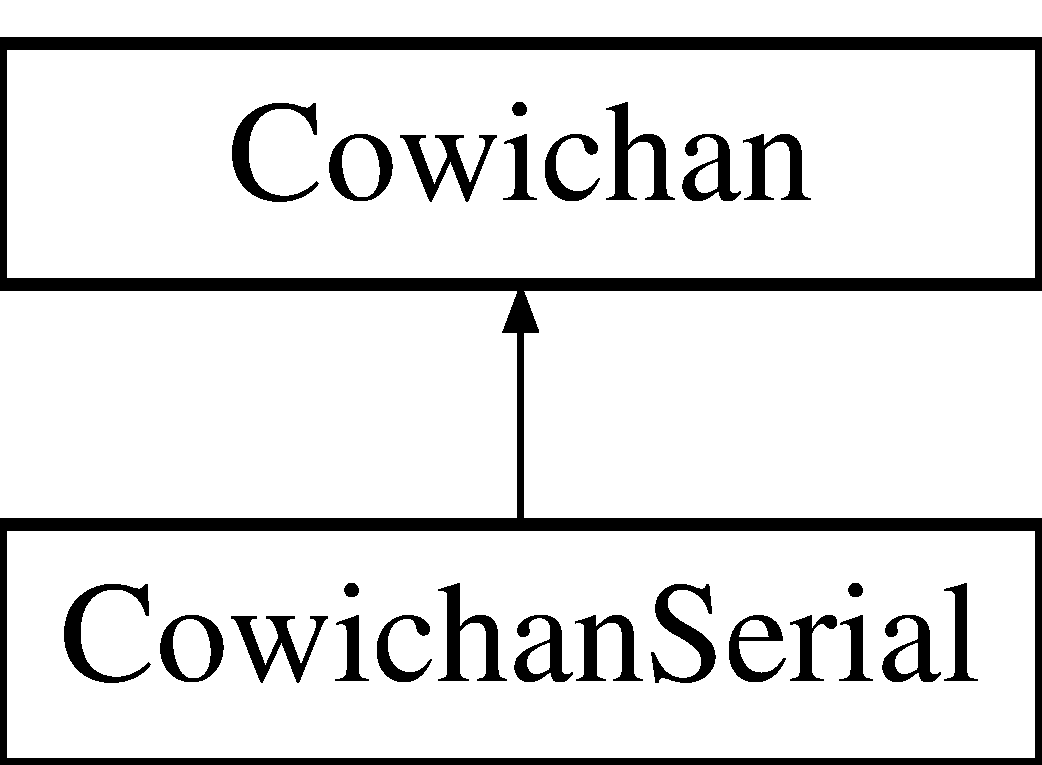
\includegraphics[height=2cm]{class_cowichan_serial}
\end{center}
\end{figure}
\subsection*{Protected Member Functions}
\begin{CompactItemize}
\item 
void \hyperlink{class_cowichan_serial_97a58b7901d8a7680cc28d42cb94d532}{mandel} (\hyperlink{cowichan_8hpp_82321152ddeeefe9c61350a42ed9e7af}{IntMatrix} matrix)
\item 
void \hyperlink{class_cowichan_serial_2d24c0e562f7b109ec2ed916f38e5911}{randmat} (\hyperlink{cowichan_8hpp_82321152ddeeefe9c61350a42ed9e7af}{IntMatrix} matrix)
\item 
void \hyperlink{class_cowichan_serial_c08a6b3e23ce26959bac12af077f924f}{half} (\hyperlink{cowichan_8hpp_82321152ddeeefe9c61350a42ed9e7af}{IntMatrix} matrixIn, \hyperlink{cowichan_8hpp_82321152ddeeefe9c61350a42ed9e7af}{IntMatrix} matrixOut)
\item 
void \hyperlink{class_cowichan_serial_9b1cf3fcbb40498609826433b8ea2f6a}{invperc} (\hyperlink{cowichan_8hpp_82321152ddeeefe9c61350a42ed9e7af}{IntMatrix} matrix, \hyperlink{cowichan_8hpp_a64c8df2f1e9c8ea68a7bcc19aca683e}{BoolMatrix} mask)
\item 
void \hyperlink{class_cowichan_serial_7c0f93b2099ce919f91b5d953ff76511}{thresh} (\hyperlink{cowichan_8hpp_82321152ddeeefe9c61350a42ed9e7af}{IntMatrix} matrix, \hyperlink{cowichan_8hpp_a64c8df2f1e9c8ea68a7bcc19aca683e}{BoolMatrix} mask)
\item 
void \hyperlink{class_cowichan_serial_ffd5b022c1d24226e11924094d8af349}{life} (\hyperlink{cowichan_8hpp_a64c8df2f1e9c8ea68a7bcc19aca683e}{BoolMatrix} matrixIn, \hyperlink{cowichan_8hpp_a64c8df2f1e9c8ea68a7bcc19aca683e}{BoolMatrix} matrixOut)
\item 
void \hyperlink{class_cowichan_serial_33daca65431f792c2f4f0e7f8d29fa01}{winnow} (\hyperlink{cowichan_8hpp_82321152ddeeefe9c61350a42ed9e7af}{IntMatrix} matrix, \hyperlink{cowichan_8hpp_a64c8df2f1e9c8ea68a7bcc19aca683e}{BoolMatrix} mask, \hyperlink{class_point}{PointVector} points)
\item 
void \hyperlink{class_cowichan_serial_0eeb47447c6a6b94ff7c6999c96fda0e}{norm} (\hyperlink{class_point}{PointVector} pointsIn, \hyperlink{class_point}{PointVector} pointsOut)
\item 
void \hyperlink{class_cowichan_serial_e75cedf0a296dd7ad3dc41cadc51776f}{hull} (\hyperlink{class_point}{PointVector} pointsIn, \hyperlink{class_point}{PointVector} pointsOut)
\item 
void \hyperlink{class_cowichan_serial_05f6899081a457d58978e4f6bda2db6a}{outer} (\hyperlink{class_point}{PointVector} points, \hyperlink{cowichan_8hpp_3fb46f939e55c239fbc95656fc0f3399}{Matrix} matrix, \hyperlink{cowichan_8hpp_02bc1553e241b9b33408482658b3c355}{Vector} vector)
\item 
void \hyperlink{class_cowichan_serial_b196d2384c2fe8b185e6269a050399eb}{gauss} (\hyperlink{cowichan_8hpp_3fb46f939e55c239fbc95656fc0f3399}{Matrix} matrix, \hyperlink{cowichan_8hpp_02bc1553e241b9b33408482658b3c355}{Vector} target, \hyperlink{cowichan_8hpp_02bc1553e241b9b33408482658b3c355}{Vector} solution)
\item 
void \hyperlink{class_cowichan_serial_6e8b06711d976de1adc1e4dc81e560e5}{sor} (\hyperlink{cowichan_8hpp_3fb46f939e55c239fbc95656fc0f3399}{Matrix} matrix, \hyperlink{cowichan_8hpp_02bc1553e241b9b33408482658b3c355}{Vector} target, \hyperlink{cowichan_8hpp_02bc1553e241b9b33408482658b3c355}{Vector} solution)
\item 
void \hyperlink{class_cowichan_serial_00411b35445d7d3038b96d53e43bdffa}{product} (\hyperlink{cowichan_8hpp_3fb46f939e55c239fbc95656fc0f3399}{Matrix} matrix, \hyperlink{cowichan_8hpp_02bc1553e241b9b33408482658b3c355}{Vector} candidate, \hyperlink{cowichan_8hpp_02bc1553e241b9b33408482658b3c355}{Vector} solution)
\item 
\hyperlink{cowichan_8hpp_4d521b2c54a1f6312cc8fa04827eaf98}{real} \hyperlink{class_cowichan_serial_34b75a2084051b3677071bb3c334d1f4}{vecdiff} (\hyperlink{cowichan_8hpp_02bc1553e241b9b33408482658b3c355}{Vector} actual, \hyperlink{cowichan_8hpp_02bc1553e241b9b33408482658b3c355}{Vector} computed)
\end{CompactItemize}


\subsection{Detailed Description}
Serial implementation. 

This implementation can serve as a reference when comparing to parallel programming systems in terms of performance, code size, complexity, etc. 

\subsection{Member Function Documentation}
\hypertarget{class_cowichan_serial_b196d2384c2fe8b185e6269a050399eb}{
\index{CowichanSerial@{CowichanSerial}!gauss@{gauss}}
\index{gauss@{gauss}!CowichanSerial@{CowichanSerial}}
\subsubsection[{gauss}]{\setlength{\rightskip}{0pt plus 5cm}void CowichanSerial::gauss ({\bf Matrix} {\em matrix}, \/  {\bf Vector} {\em target}, \/  {\bf Vector} {\em solution})\hspace{0.3cm}{\tt  \mbox{[}protected, virtual\mbox{]}}}}
\label{class_cowichan_serial_b196d2384c2fe8b185e6269a050399eb}


For description see \hyperlink{index_gauss_sec}{11. Gaussian Elimination} \begin{Desc}
\item[Parameters:]
\begin{description}
\item[{\em matrix}]matrix A in AX = V. \item[{\em target}]vector V in AX = V. \item[{\em solution}]vector X in AX = V. \end{description}
\end{Desc}


Implements \hyperlink{class_cowichan_aa9aac74b96dc5ed33e821d94649d1b2}{Cowichan}.\hypertarget{class_cowichan_serial_c08a6b3e23ce26959bac12af077f924f}{
\index{CowichanSerial@{CowichanSerial}!half@{half}}
\index{half@{half}!CowichanSerial@{CowichanSerial}}
\subsubsection[{half}]{\setlength{\rightskip}{0pt plus 5cm}void CowichanSerial::half ({\bf IntMatrix} {\em matrixIn}, \/  {\bf IntMatrix} {\em matrixOut})\hspace{0.3cm}{\tt  \mbox{[}protected, virtual\mbox{]}}}}
\label{class_cowichan_serial_c08a6b3e23ce26959bac12af077f924f}


For description see \hyperlink{index_half_sec}{3. Two-Dimensional Shuffle} \begin{Desc}
\item[Parameters:]
\begin{description}
\item[{\em matrixIn}]matrix to shuffle. \item[{\em matrixOut}]shuffled matrix. \end{description}
\end{Desc}


Implements \hyperlink{class_cowichan_308603053675bccbe631f04af921f57c}{Cowichan}.\hypertarget{class_cowichan_serial_e75cedf0a296dd7ad3dc41cadc51776f}{
\index{CowichanSerial@{CowichanSerial}!hull@{hull}}
\index{hull@{hull}!CowichanSerial@{CowichanSerial}}
\subsubsection[{hull}]{\setlength{\rightskip}{0pt plus 5cm}void CowichanSerial::hull ({\bf PointVector} {\em pointsIn}, \/  {\bf PointVector} {\em pointsOut})\hspace{0.3cm}{\tt  \mbox{[}protected, virtual\mbox{]}}}}
\label{class_cowichan_serial_e75cedf0a296dd7ad3dc41cadc51776f}


Runs quickhull algorithm until all points have been used up from the original vector. At each step the hull points are marked as used and a new convex hull is computed on the rest of points. The points that have been used up are in the range (n - hn, n), i.e. at the end of pointsIn vector. NOTE: pointsIn vector gets modified by the algorithm. 

Implements \hyperlink{class_cowichan_0c6b68ae3c059b66893405f8530a2e0a}{Cowichan}.\hypertarget{class_cowichan_serial_9b1cf3fcbb40498609826433b8ea2f6a}{
\index{CowichanSerial@{CowichanSerial}!invperc@{invperc}}
\index{invperc@{invperc}!CowichanSerial@{CowichanSerial}}
\subsubsection[{invperc}]{\setlength{\rightskip}{0pt plus 5cm}void CowichanSerial::invperc ({\bf IntMatrix} {\em matrix}, \/  {\bf BoolMatrix} {\em mask})\hspace{0.3cm}{\tt  \mbox{[}protected, virtual\mbox{]}}}}
\label{class_cowichan_serial_9b1cf3fcbb40498609826433b8ea2f6a}


For description see \hyperlink{index_invperc_sec}{4. Invasion Percolation} \begin{Desc}
\item[Parameters:]
\begin{description}
\item[{\em matrix}]filling resistance matrix. \item[{\em mask}]filled cells. \end{description}
\end{Desc}


Implements \hyperlink{class_cowichan_ea126792a31e54a8722663b7ea768955}{Cowichan}.\hypertarget{class_cowichan_serial_ffd5b022c1d24226e11924094d8af349}{
\index{CowichanSerial@{CowichanSerial}!life@{life}}
\index{life@{life}!CowichanSerial@{CowichanSerial}}
\subsubsection[{life}]{\setlength{\rightskip}{0pt plus 5cm}void CowichanSerial::life ({\bf BoolMatrix} {\em matrixIn}, \/  {\bf BoolMatrix} {\em matrixOut})\hspace{0.3cm}{\tt  \mbox{[}protected, virtual\mbox{]}}}}
\label{class_cowichan_serial_ffd5b022c1d24226e11924094d8af349}


For description see \hyperlink{index_life_sec}{6. Game of Life} \begin{Desc}
\item[Parameters:]
\begin{description}
\item[{\em matrixIn}]initial world. \item[{\em matrixOut}]final world. \end{description}
\end{Desc}


Implements \hyperlink{class_cowichan_d449595ef2fe934bdd128ac8b1f51d07}{Cowichan}.\hypertarget{class_cowichan_serial_97a58b7901d8a7680cc28d42cb94d532}{
\index{CowichanSerial@{CowichanSerial}!mandel@{mandel}}
\index{mandel@{mandel}!CowichanSerial@{CowichanSerial}}
\subsubsection[{mandel}]{\setlength{\rightskip}{0pt plus 5cm}void CowichanSerial::mandel ({\bf IntMatrix} {\em matrix})\hspace{0.3cm}{\tt  \mbox{[}protected, virtual\mbox{]}}}}
\label{class_cowichan_serial_97a58b7901d8a7680cc28d42cb94d532}


For description see \hyperlink{index_mandel_sec}{1. Mandelbrot Set Generation} \begin{Desc}
\item[Parameters:]
\begin{description}
\item[{\em matrix}]matrix to fill. \end{description}
\end{Desc}


Implements \hyperlink{class_cowichan_ec6cc4eb2ad444474b923532167e98a2}{Cowichan}.\hypertarget{class_cowichan_serial_0eeb47447c6a6b94ff7c6999c96fda0e}{
\index{CowichanSerial@{CowichanSerial}!norm@{norm}}
\index{norm@{norm}!CowichanSerial@{CowichanSerial}}
\subsubsection[{norm}]{\setlength{\rightskip}{0pt plus 5cm}void CowichanSerial::norm ({\bf PointVector} {\em pointsIn}, \/  {\bf PointVector} {\em pointsOut})\hspace{0.3cm}{\tt  \mbox{[}protected, virtual\mbox{]}}}}
\label{class_cowichan_serial_0eeb47447c6a6b94ff7c6999c96fda0e}


For description see \hyperlink{index_norm_sec}{8. Point Location Normalization} \begin{Desc}
\item[Parameters:]
\begin{description}
\item[{\em pointsIn}]points to normalize. \item[{\em pointsOut}]normalized points. \end{description}
\end{Desc}


Implements \hyperlink{class_cowichan_3df21e3c627958114e045c3559a29f30}{Cowichan}.\hypertarget{class_cowichan_serial_05f6899081a457d58978e4f6bda2db6a}{
\index{CowichanSerial@{CowichanSerial}!outer@{outer}}
\index{outer@{outer}!CowichanSerial@{CowichanSerial}}
\subsubsection[{outer}]{\setlength{\rightskip}{0pt plus 5cm}void CowichanSerial::outer ({\bf PointVector} {\em points}, \/  {\bf Matrix} {\em matrix}, \/  {\bf Vector} {\em vector})\hspace{0.3cm}{\tt  \mbox{[}protected, virtual\mbox{]}}}}
\label{class_cowichan_serial_05f6899081a457d58978e4f6bda2db6a}


For description see \hyperlink{index_outer_sec}{10. Outer Product} \begin{Desc}
\item[Parameters:]
\begin{description}
\item[{\em points}]vector of points. \item[{\em matrix}]resulting distance matrix. \item[{\em vector}]resulting distance vector. \end{description}
\end{Desc}


Implements \hyperlink{class_cowichan_52f17221019290b88334b0ca7f3bcdb9}{Cowichan}.\hypertarget{class_cowichan_serial_00411b35445d7d3038b96d53e43bdffa}{
\index{CowichanSerial@{CowichanSerial}!product@{product}}
\index{product@{product}!CowichanSerial@{CowichanSerial}}
\subsubsection[{product}]{\setlength{\rightskip}{0pt plus 5cm}void CowichanSerial::product ({\bf Matrix} {\em matrix}, \/  {\bf Vector} {\em candidate}, \/  {\bf Vector} {\em solution})\hspace{0.3cm}{\tt  \mbox{[}protected, virtual\mbox{]}}}}
\label{class_cowichan_serial_00411b35445d7d3038b96d53e43bdffa}


For description see \hyperlink{index_product_sec}{13. Matrix-Vector Product} \begin{Desc}
\item[Parameters:]
\begin{description}
\item[{\em matrix}]matrix A in AX = V. \item[{\em candidate}]vector X in AX = V. \item[{\em solution}]vector V in AX = V. \end{description}
\end{Desc}


Implements \hyperlink{class_cowichan_3d7d4b581a1d6f0392dc452830fb3b03}{Cowichan}.\hypertarget{class_cowichan_serial_2d24c0e562f7b109ec2ed916f38e5911}{
\index{CowichanSerial@{CowichanSerial}!randmat@{randmat}}
\index{randmat@{randmat}!CowichanSerial@{CowichanSerial}}
\subsubsection[{randmat}]{\setlength{\rightskip}{0pt plus 5cm}void CowichanSerial::randmat ({\bf IntMatrix} {\em matrix})\hspace{0.3cm}{\tt  \mbox{[}protected, virtual\mbox{]}}}}
\label{class_cowichan_serial_2d24c0e562f7b109ec2ed916f38e5911}


For description see \hyperlink{index_randmat_sec}{2. Random Number Generation} \begin{Desc}
\item[Parameters:]
\begin{description}
\item[{\em matrix}]matrix to fill. \end{description}
\end{Desc}


Implements \hyperlink{class_cowichan_c44cacf9d9e363a5b076bcee8b9a7a73}{Cowichan}.\hypertarget{class_cowichan_serial_6e8b06711d976de1adc1e4dc81e560e5}{
\index{CowichanSerial@{CowichanSerial}!sor@{sor}}
\index{sor@{sor}!CowichanSerial@{CowichanSerial}}
\subsubsection[{sor}]{\setlength{\rightskip}{0pt plus 5cm}void CowichanSerial::sor ({\bf Matrix} {\em matrix}, \/  {\bf Vector} {\em target}, \/  {\bf Vector} {\em solution})\hspace{0.3cm}{\tt  \mbox{[}protected, virtual\mbox{]}}}}
\label{class_cowichan_serial_6e8b06711d976de1adc1e4dc81e560e5}


For description see \hyperlink{index_sor_sec}{12. Successive Over-Relaxation} \begin{Desc}
\item[Parameters:]
\begin{description}
\item[{\em matrix}]matrix A in AX = V. \item[{\em target}]vector V in AX = V. \item[{\em solution}]vector X in AX = V. \end{description}
\end{Desc}


Implements \hyperlink{class_cowichan_92d8d9ae77208115fdfe69e1174f601c}{Cowichan}.\hypertarget{class_cowichan_serial_7c0f93b2099ce919f91b5d953ff76511}{
\index{CowichanSerial@{CowichanSerial}!thresh@{thresh}}
\index{thresh@{thresh}!CowichanSerial@{CowichanSerial}}
\subsubsection[{thresh}]{\setlength{\rightskip}{0pt plus 5cm}void CowichanSerial::thresh ({\bf IntMatrix} {\em matrix}, \/  {\bf BoolMatrix} {\em mask})\hspace{0.3cm}{\tt  \mbox{[}protected, virtual\mbox{]}}}}
\label{class_cowichan_serial_7c0f93b2099ce919f91b5d953ff76511}


Works only on positive input. 

Implements \hyperlink{class_cowichan_a0b633b8c1f21884e0998a9c7020c08c}{Cowichan}.\hypertarget{class_cowichan_serial_34b75a2084051b3677071bb3c334d1f4}{
\index{CowichanSerial@{CowichanSerial}!vecdiff@{vecdiff}}
\index{vecdiff@{vecdiff}!CowichanSerial@{CowichanSerial}}
\subsubsection[{vecdiff}]{\setlength{\rightskip}{0pt plus 5cm}{\bf real} CowichanSerial::vecdiff ({\bf Vector} {\em actual}, \/  {\bf Vector} {\em computed})\hspace{0.3cm}{\tt  \mbox{[}protected, virtual\mbox{]}}}}
\label{class_cowichan_serial_34b75a2084051b3677071bb3c334d1f4}


For description see \hyperlink{index_vecdiff_sec}{14. 1-Norm Vector Difference} \begin{Desc}
\item[Parameters:]
\begin{description}
\item[{\em actual}]first vector. \item[{\em computed}]second vector. \end{description}
\end{Desc}


Implements \hyperlink{class_cowichan_775d72b5e7d122f9f32555352278250e}{Cowichan}.\hypertarget{class_cowichan_serial_33daca65431f792c2f4f0e7f8d29fa01}{
\index{CowichanSerial@{CowichanSerial}!winnow@{winnow}}
\index{winnow@{winnow}!CowichanSerial@{CowichanSerial}}
\subsubsection[{winnow}]{\setlength{\rightskip}{0pt plus 5cm}void CowichanSerial::winnow ({\bf IntMatrix} {\em matrix}, \/  {\bf BoolMatrix} {\em mask}, \/  {\bf PointVector} {\em points})\hspace{0.3cm}{\tt  \mbox{[}protected, virtual\mbox{]}}}}
\label{class_cowichan_serial_33daca65431f792c2f4f0e7f8d29fa01}


For description see \hyperlink{index_winnow_sec}{7. Weighted Point Selection} \begin{Desc}
\item[Parameters:]
\begin{description}
\item[{\em matrix}]integer matrix. \item[{\em mask}]boolean matrix. \item[{\em points}]evenly selected points. \end{description}
\end{Desc}


Implements \hyperlink{class_cowichan_13d60e06ced3b5da79d62c133ce82337}{Cowichan}.

The documentation for this class was generated from the following files:\begin{CompactItemize}
\item 
cowichan\_\-serial/\hyperlink{cowichan__serial_8hpp}{cowichan\_\-serial.hpp}\item 
cowichan\_\-serial/\hyperlink{cowichan__serial_2gauss_8cpp}{gauss.cpp}\item 
cowichan\_\-serial/\hyperlink{cowichan__serial_2half_8cpp}{half.cpp}\item 
cowichan\_\-serial/\hyperlink{cowichan__serial_2hull_8cpp}{hull.cpp}\item 
cowichan\_\-serial/\hyperlink{cowichan__serial_2invperc_8cpp}{invperc.cpp}\item 
cowichan\_\-serial/\hyperlink{cowichan__serial_2life_8cpp}{life.cpp}\item 
cowichan\_\-serial/\hyperlink{cowichan__serial_2mandel_8cpp}{mandel.cpp}\item 
cowichan\_\-serial/\hyperlink{cowichan__serial_2norm_8cpp}{norm.cpp}\item 
cowichan\_\-serial/\hyperlink{cowichan__serial_2outer_8cpp}{outer.cpp}\item 
cowichan\_\-serial/\hyperlink{cowichan__serial_2product_8cpp}{product.cpp}\item 
cowichan\_\-serial/\hyperlink{cowichan__serial_2randmat_8cpp}{randmat.cpp}\item 
cowichan\_\-serial/\hyperlink{cowichan__serial_2sor_8cpp}{sor.cpp}\item 
cowichan\_\-serial/\hyperlink{cowichan__serial_2thresh_8cpp}{thresh.cpp}\item 
cowichan\_\-serial/\hyperlink{cowichan__serial_2vecdiff_8cpp}{vecdiff.cpp}\item 
cowichan\_\-serial/\hyperlink{cowichan__serial_2winnow_8cpp}{winnow.cpp}\end{CompactItemize}

\hypertarget{class_cowichan_t_b_b}{
\section{CowichanTBB Class Reference}
\label{class_cowichan_t_b_b}\index{CowichanTBB@{CowichanTBB}}
}
Thread Building Blocks (TBB) implementation.  


{\tt \#include $<$cowichan\_\-tbb.hpp$>$}

Inheritance diagram for CowichanTBB::\begin{figure}[H]
\begin{center}
\leavevmode
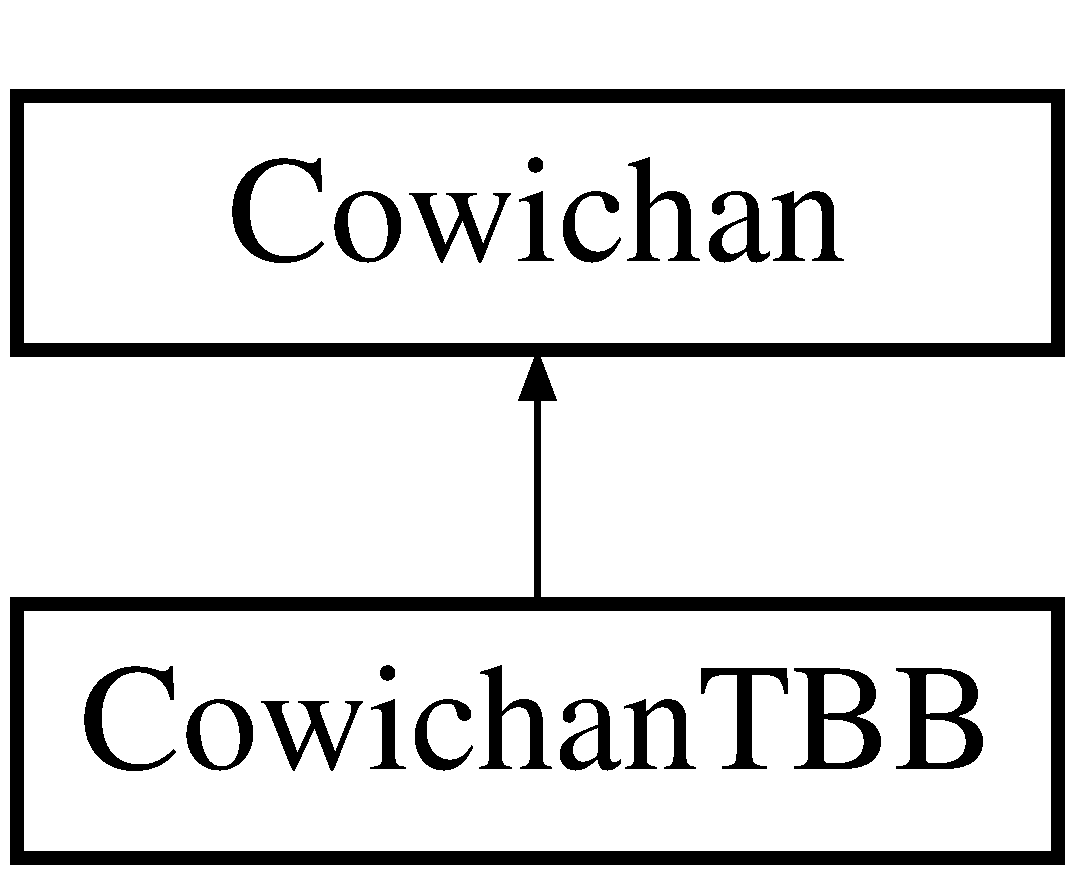
\includegraphics[height=2cm]{class_cowichan_t_b_b}
\end{center}
\end{figure}
\subsection*{Protected Member Functions}
\begin{CompactItemize}
\item 
void \hyperlink{class_cowichan_t_b_b_1e58b60ff22a58aba69567ecc6740878}{mandel} (\hyperlink{cowichan_8hpp_82321152ddeeefe9c61350a42ed9e7af}{IntMatrix} matrix)
\item 
void \hyperlink{class_cowichan_t_b_b_b9b5cb4b4b5dc8907b2a01825cd4aaff}{randmat} (\hyperlink{cowichan_8hpp_82321152ddeeefe9c61350a42ed9e7af}{IntMatrix} matrix)
\item 
void \hyperlink{class_cowichan_t_b_b_bbf17e641657d54fc0c571c008ac8f7a}{half} (\hyperlink{cowichan_8hpp_82321152ddeeefe9c61350a42ed9e7af}{IntMatrix} matrixIn, \hyperlink{cowichan_8hpp_82321152ddeeefe9c61350a42ed9e7af}{IntMatrix} matrixOut)
\item 
void \hyperlink{class_cowichan_t_b_b_e4f9f8c31feea9b3a167fc2880a97610}{invperc} (\hyperlink{cowichan_8hpp_82321152ddeeefe9c61350a42ed9e7af}{IntMatrix} matrix, \hyperlink{cowichan_8hpp_a64c8df2f1e9c8ea68a7bcc19aca683e}{BoolMatrix} mask)
\item 
void \hyperlink{class_cowichan_t_b_b_3306d21f0b3d12cc2e3b050b99812a27}{thresh} (\hyperlink{cowichan_8hpp_82321152ddeeefe9c61350a42ed9e7af}{IntMatrix} matrix, \hyperlink{cowichan_8hpp_a64c8df2f1e9c8ea68a7bcc19aca683e}{BoolMatrix} mask)
\item 
void \hyperlink{class_cowichan_t_b_b_273e3e8a2e05108f59ec613472bfa363}{life} (\hyperlink{cowichan_8hpp_a64c8df2f1e9c8ea68a7bcc19aca683e}{BoolMatrix} matrixIn, \hyperlink{cowichan_8hpp_a64c8df2f1e9c8ea68a7bcc19aca683e}{BoolMatrix} matrixOut)
\item 
void \hyperlink{class_cowichan_t_b_b_77178470ef780e0505137dc1d22a85a2}{winnow} (\hyperlink{cowichan_8hpp_82321152ddeeefe9c61350a42ed9e7af}{IntMatrix} matrix, \hyperlink{cowichan_8hpp_a64c8df2f1e9c8ea68a7bcc19aca683e}{BoolMatrix} mask, \hyperlink{class_point}{PointVector} points)
\item 
void \hyperlink{class_cowichan_t_b_b_ca08645b51a242317a115cd7ce7d81fe}{norm} (\hyperlink{class_point}{PointVector} pointsIn, \hyperlink{class_point}{PointVector} pointsOut)
\item 
void \hyperlink{class_cowichan_t_b_b_0d23aa05dc21fd9e8b033769097b4b18}{hull} (\hyperlink{class_point}{PointVector} pointsIn, \hyperlink{class_point}{PointVector} pointsOut)
\item 
void \hyperlink{class_cowichan_t_b_b_92a763b9733cdcceda13b7b7ea0bc229}{outer} (\hyperlink{class_point}{PointVector} points, \hyperlink{cowichan_8hpp_3fb46f939e55c239fbc95656fc0f3399}{Matrix} matrix, \hyperlink{cowichan_8hpp_02bc1553e241b9b33408482658b3c355}{Vector} vector)
\item 
void \hyperlink{class_cowichan_t_b_b_d51868e0e65482f7c9e69d73b3904822}{gauss} (\hyperlink{cowichan_8hpp_3fb46f939e55c239fbc95656fc0f3399}{Matrix} matrix, \hyperlink{cowichan_8hpp_02bc1553e241b9b33408482658b3c355}{Vector} target, \hyperlink{cowichan_8hpp_02bc1553e241b9b33408482658b3c355}{Vector} solution)
\item 
void \hyperlink{class_cowichan_t_b_b_dbb32ce457d0edca6815ab1cb2459276}{sor} (\hyperlink{cowichan_8hpp_3fb46f939e55c239fbc95656fc0f3399}{Matrix} matrix, \hyperlink{cowichan_8hpp_02bc1553e241b9b33408482658b3c355}{Vector} target, \hyperlink{cowichan_8hpp_02bc1553e241b9b33408482658b3c355}{Vector} solution)
\item 
void \hyperlink{class_cowichan_t_b_b_f3144458520e2dff1f9fad5753f6fc3d}{product} (\hyperlink{cowichan_8hpp_3fb46f939e55c239fbc95656fc0f3399}{Matrix} matrix, \hyperlink{cowichan_8hpp_02bc1553e241b9b33408482658b3c355}{Vector} candidate, \hyperlink{cowichan_8hpp_02bc1553e241b9b33408482658b3c355}{Vector} solution)
\item 
\hyperlink{cowichan_8hpp_4d521b2c54a1f6312cc8fa04827eaf98}{real} \hyperlink{class_cowichan_t_b_b_28c976743df231fd183e4db9306050b1}{vecdiff} (\hyperlink{cowichan_8hpp_02bc1553e241b9b33408482658b3c355}{Vector} actual, \hyperlink{cowichan_8hpp_02bc1553e241b9b33408482658b3c355}{Vector} computed)
\end{CompactItemize}


\subsection{Detailed Description}
Thread Building Blocks (TBB) implementation. 

Tags: shared memory, data parallel, task based. 

\subsection{Member Function Documentation}
\hypertarget{class_cowichan_t_b_b_d51868e0e65482f7c9e69d73b3904822}{
\index{CowichanTBB@{CowichanTBB}!gauss@{gauss}}
\index{gauss@{gauss}!CowichanTBB@{CowichanTBB}}
\subsubsection[{gauss}]{\setlength{\rightskip}{0pt plus 5cm}void CowichanTBB::gauss ({\bf Matrix} {\em matrix}, \/  {\bf Vector} {\em target}, \/  {\bf Vector} {\em solution})\hspace{0.3cm}{\tt  \mbox{[}protected, virtual\mbox{]}}}}
\label{class_cowichan_t_b_b_d51868e0e65482f7c9e69d73b3904822}


For description see \hyperlink{index_gauss_sec}{11. Gaussian Elimination} \begin{Desc}
\item[Parameters:]
\begin{description}
\item[{\em matrix}]matrix A in AX = V. \item[{\em target}]vector V in AX = V. \item[{\em solution}]vector X in AX = V. \end{description}
\end{Desc}


Implements \hyperlink{class_cowichan_aa9aac74b96dc5ed33e821d94649d1b2}{Cowichan}.\hypertarget{class_cowichan_t_b_b_bbf17e641657d54fc0c571c008ac8f7a}{
\index{CowichanTBB@{CowichanTBB}!half@{half}}
\index{half@{half}!CowichanTBB@{CowichanTBB}}
\subsubsection[{half}]{\setlength{\rightskip}{0pt plus 5cm}void CowichanTBB::half ({\bf IntMatrix} {\em matrixIn}, \/  {\bf IntMatrix} {\em matrixOut})\hspace{0.3cm}{\tt  \mbox{[}protected, virtual\mbox{]}}}}
\label{class_cowichan_t_b_b_bbf17e641657d54fc0c571c008ac8f7a}


For description see \hyperlink{index_half_sec}{3. Two-Dimensional Shuffle} \begin{Desc}
\item[Parameters:]
\begin{description}
\item[{\em matrixIn}]matrix to shuffle. \item[{\em matrixOut}]shuffled matrix. \end{description}
\end{Desc}


Implements \hyperlink{class_cowichan_308603053675bccbe631f04af921f57c}{Cowichan}.\hypertarget{class_cowichan_t_b_b_0d23aa05dc21fd9e8b033769097b4b18}{
\index{CowichanTBB@{CowichanTBB}!hull@{hull}}
\index{hull@{hull}!CowichanTBB@{CowichanTBB}}
\subsubsection[{hull}]{\setlength{\rightskip}{0pt plus 5cm}void CowichanTBB::hull ({\bf PointVector} {\em pointsIn}, \/  {\bf PointVector} {\em pointsOut})\hspace{0.3cm}{\tt  \mbox{[}protected, virtual\mbox{]}}}}
\label{class_cowichan_t_b_b_0d23aa05dc21fd9e8b033769097b4b18}


For description see \hyperlink{index_hull_sec}{9. Convex Hull}

Runs quickhull algorithm until all points have been used up from the original vector. At each step the hull points are marked as used and a new convex hull is computed on the rest of points. The points that have been used up are in the range (n - hn, n), i.e. at the end of pointsIn vector. NOTE: pointsIn vector gets modified by the algorithm. 

Implements \hyperlink{class_cowichan_0c6b68ae3c059b66893405f8530a2e0a}{Cowichan}.\hypertarget{class_cowichan_t_b_b_e4f9f8c31feea9b3a167fc2880a97610}{
\index{CowichanTBB@{CowichanTBB}!invperc@{invperc}}
\index{invperc@{invperc}!CowichanTBB@{CowichanTBB}}
\subsubsection[{invperc}]{\setlength{\rightskip}{0pt plus 5cm}void CowichanTBB::invperc ({\bf IntMatrix} {\em matrix}, \/  {\bf BoolMatrix} {\em mask})\hspace{0.3cm}{\tt  \mbox{[}protected, virtual\mbox{]}}}}
\label{class_cowichan_t_b_b_e4f9f8c31feea9b3a167fc2880a97610}


For description see \hyperlink{index_invperc_sec}{4. Invasion Percolation} \begin{Desc}
\item[Parameters:]
\begin{description}
\item[{\em matrix}]filling resistance matrix. \item[{\em mask}]filled cells. \end{description}
\end{Desc}


Implements \hyperlink{class_cowichan_ea126792a31e54a8722663b7ea768955}{Cowichan}.\hypertarget{class_cowichan_t_b_b_273e3e8a2e05108f59ec613472bfa363}{
\index{CowichanTBB@{CowichanTBB}!life@{life}}
\index{life@{life}!CowichanTBB@{CowichanTBB}}
\subsubsection[{life}]{\setlength{\rightskip}{0pt plus 5cm}void CowichanTBB::life ({\bf BoolMatrix} {\em matrixIn}, \/  {\bf BoolMatrix} {\em matrixOut})\hspace{0.3cm}{\tt  \mbox{[}protected, virtual\mbox{]}}}}
\label{class_cowichan_t_b_b_273e3e8a2e05108f59ec613472bfa363}


For description see \hyperlink{index_life_sec}{6. Game of Life} \begin{Desc}
\item[Parameters:]
\begin{description}
\item[{\em matrixIn}]initial world. \item[{\em matrixOut}]final world. \end{description}
\end{Desc}


Implements \hyperlink{class_cowichan_d449595ef2fe934bdd128ac8b1f51d07}{Cowichan}.\hypertarget{class_cowichan_t_b_b_1e58b60ff22a58aba69567ecc6740878}{
\index{CowichanTBB@{CowichanTBB}!mandel@{mandel}}
\index{mandel@{mandel}!CowichanTBB@{CowichanTBB}}
\subsubsection[{mandel}]{\setlength{\rightskip}{0pt plus 5cm}void CowichanTBB::mandel ({\bf IntMatrix} {\em matrix})\hspace{0.3cm}{\tt  \mbox{[}protected, virtual\mbox{]}}}}
\label{class_cowichan_t_b_b_1e58b60ff22a58aba69567ecc6740878}


For description see \hyperlink{index_mandel_sec}{1. Mandelbrot Set Generation} \begin{Desc}
\item[Parameters:]
\begin{description}
\item[{\em matrix}]matrix to fill. \end{description}
\end{Desc}


Implements \hyperlink{class_cowichan_ec6cc4eb2ad444474b923532167e98a2}{Cowichan}.\hypertarget{class_cowichan_t_b_b_ca08645b51a242317a115cd7ce7d81fe}{
\index{CowichanTBB@{CowichanTBB}!norm@{norm}}
\index{norm@{norm}!CowichanTBB@{CowichanTBB}}
\subsubsection[{norm}]{\setlength{\rightskip}{0pt plus 5cm}void CowichanTBB::norm ({\bf PointVector} {\em pointsIn}, \/  {\bf PointVector} {\em pointsOut})\hspace{0.3cm}{\tt  \mbox{[}protected, virtual\mbox{]}}}}
\label{class_cowichan_t_b_b_ca08645b51a242317a115cd7ce7d81fe}


For description see \hyperlink{index_norm_sec}{8. Point Location Normalization} \begin{Desc}
\item[Parameters:]
\begin{description}
\item[{\em pointsIn}]points to normalize. \item[{\em pointsOut}]normalized points. \end{description}
\end{Desc}


Implements \hyperlink{class_cowichan_3df21e3c627958114e045c3559a29f30}{Cowichan}.\hypertarget{class_cowichan_t_b_b_92a763b9733cdcceda13b7b7ea0bc229}{
\index{CowichanTBB@{CowichanTBB}!outer@{outer}}
\index{outer@{outer}!CowichanTBB@{CowichanTBB}}
\subsubsection[{outer}]{\setlength{\rightskip}{0pt plus 5cm}void CowichanTBB::outer ({\bf PointVector} {\em points}, \/  {\bf Matrix} {\em matrix}, \/  {\bf Vector} {\em vector})\hspace{0.3cm}{\tt  \mbox{[}protected, virtual\mbox{]}}}}
\label{class_cowichan_t_b_b_92a763b9733cdcceda13b7b7ea0bc229}


For description see \hyperlink{index_outer_sec}{10. Outer Product} \begin{Desc}
\item[Parameters:]
\begin{description}
\item[{\em points}]vector of points. \item[{\em matrix}]resulting distance matrix. \item[{\em vector}]resulting distance vector. \end{description}
\end{Desc}


Implements \hyperlink{class_cowichan_52f17221019290b88334b0ca7f3bcdb9}{Cowichan}.\hypertarget{class_cowichan_t_b_b_f3144458520e2dff1f9fad5753f6fc3d}{
\index{CowichanTBB@{CowichanTBB}!product@{product}}
\index{product@{product}!CowichanTBB@{CowichanTBB}}
\subsubsection[{product}]{\setlength{\rightskip}{0pt plus 5cm}void CowichanTBB::product ({\bf Matrix} {\em matrix}, \/  {\bf Vector} {\em candidate}, \/  {\bf Vector} {\em solution})\hspace{0.3cm}{\tt  \mbox{[}protected, virtual\mbox{]}}}}
\label{class_cowichan_t_b_b_f3144458520e2dff1f9fad5753f6fc3d}


For description see \hyperlink{index_product_sec}{13. Matrix-Vector Product} \begin{Desc}
\item[Parameters:]
\begin{description}
\item[{\em matrix}]matrix A in AX = V. \item[{\em candidate}]vector X in AX = V. \item[{\em solution}]vector V in AX = V. \end{description}
\end{Desc}


Implements \hyperlink{class_cowichan_3d7d4b581a1d6f0392dc452830fb3b03}{Cowichan}.\hypertarget{class_cowichan_t_b_b_b9b5cb4b4b5dc8907b2a01825cd4aaff}{
\index{CowichanTBB@{CowichanTBB}!randmat@{randmat}}
\index{randmat@{randmat}!CowichanTBB@{CowichanTBB}}
\subsubsection[{randmat}]{\setlength{\rightskip}{0pt plus 5cm}void CowichanTBB::randmat ({\bf IntMatrix} {\em matrix})\hspace{0.3cm}{\tt  \mbox{[}protected, virtual\mbox{]}}}}
\label{class_cowichan_t_b_b_b9b5cb4b4b5dc8907b2a01825cd4aaff}


For description see \hyperlink{index_randmat_sec}{2. Random Number Generation} \begin{Desc}
\item[Parameters:]
\begin{description}
\item[{\em matrix}]matrix to fill. \end{description}
\end{Desc}


Implements \hyperlink{class_cowichan_c44cacf9d9e363a5b076bcee8b9a7a73}{Cowichan}.\hypertarget{class_cowichan_t_b_b_dbb32ce457d0edca6815ab1cb2459276}{
\index{CowichanTBB@{CowichanTBB}!sor@{sor}}
\index{sor@{sor}!CowichanTBB@{CowichanTBB}}
\subsubsection[{sor}]{\setlength{\rightskip}{0pt plus 5cm}void CowichanTBB::sor ({\bf Matrix} {\em matrix}, \/  {\bf Vector} {\em target}, \/  {\bf Vector} {\em solution})\hspace{0.3cm}{\tt  \mbox{[}protected, virtual\mbox{]}}}}
\label{class_cowichan_t_b_b_dbb32ce457d0edca6815ab1cb2459276}


For description see \hyperlink{index_sor_sec}{12. Successive Over-Relaxation} \begin{Desc}
\item[Parameters:]
\begin{description}
\item[{\em matrix}]matrix A in AX = V. \item[{\em target}]vector V in AX = V. \item[{\em solution}]vector X in AX = V. \end{description}
\end{Desc}


Implements \hyperlink{class_cowichan_92d8d9ae77208115fdfe69e1174f601c}{Cowichan}.\hypertarget{class_cowichan_t_b_b_3306d21f0b3d12cc2e3b050b99812a27}{
\index{CowichanTBB@{CowichanTBB}!thresh@{thresh}}
\index{thresh@{thresh}!CowichanTBB@{CowichanTBB}}
\subsubsection[{thresh}]{\setlength{\rightskip}{0pt plus 5cm}void CowichanTBB::thresh ({\bf IntMatrix} {\em matrix}, \/  {\bf BoolMatrix} {\em mask})\hspace{0.3cm}{\tt  \mbox{[}protected, virtual\mbox{]}}}}
\label{class_cowichan_t_b_b_3306d21f0b3d12cc2e3b050b99812a27}


For description see \hyperlink{index_thresh_sec}{5. Histogram Thresholding} \begin{Desc}
\item[Parameters:]
\begin{description}
\item[{\em matrix}]image. \item[{\em mask}]image after thresholding. \end{description}
\end{Desc}


Implements \hyperlink{class_cowichan_a0b633b8c1f21884e0998a9c7020c08c}{Cowichan}.\hypertarget{class_cowichan_t_b_b_28c976743df231fd183e4db9306050b1}{
\index{CowichanTBB@{CowichanTBB}!vecdiff@{vecdiff}}
\index{vecdiff@{vecdiff}!CowichanTBB@{CowichanTBB}}
\subsubsection[{vecdiff}]{\setlength{\rightskip}{0pt plus 5cm}{\bf real} CowichanTBB::vecdiff ({\bf Vector} {\em actual}, \/  {\bf Vector} {\em computed})\hspace{0.3cm}{\tt  \mbox{[}protected, virtual\mbox{]}}}}
\label{class_cowichan_t_b_b_28c976743df231fd183e4db9306050b1}


For description see \hyperlink{index_vecdiff_sec}{14. 1-Norm Vector Difference} \begin{Desc}
\item[Parameters:]
\begin{description}
\item[{\em actual}]first vector. \item[{\em computed}]second vector. \end{description}
\end{Desc}


Implements \hyperlink{class_cowichan_775d72b5e7d122f9f32555352278250e}{Cowichan}.\hypertarget{class_cowichan_t_b_b_77178470ef780e0505137dc1d22a85a2}{
\index{CowichanTBB@{CowichanTBB}!winnow@{winnow}}
\index{winnow@{winnow}!CowichanTBB@{CowichanTBB}}
\subsubsection[{winnow}]{\setlength{\rightskip}{0pt plus 5cm}void CowichanTBB::winnow ({\bf IntMatrix} {\em matrix}, \/  {\bf BoolMatrix} {\em mask}, \/  {\bf PointVector} {\em points})\hspace{0.3cm}{\tt  \mbox{[}protected, virtual\mbox{]}}}}
\label{class_cowichan_t_b_b_77178470ef780e0505137dc1d22a85a2}


For description see \hyperlink{index_winnow_sec}{7. Weighted Point Selection} \begin{Desc}
\item[Parameters:]
\begin{description}
\item[{\em matrix}]integer matrix. \item[{\em mask}]boolean matrix. \item[{\em points}]evenly selected points. \end{description}
\end{Desc}


Implements \hyperlink{class_cowichan_13d60e06ced3b5da79d62c133ce82337}{Cowichan}.

The documentation for this class was generated from the following files:\begin{CompactItemize}
\item 
cowichan\_\-tbb/\hyperlink{cowichan__tbb_8hpp}{cowichan\_\-tbb.hpp}\item 
cowichan\_\-tbb/\hyperlink{cowichan__tbb_2gauss_8cpp}{gauss.cpp}\item 
cowichan\_\-tbb/\hyperlink{cowichan__tbb_2half_8cpp}{half.cpp}\item 
cowichan\_\-tbb/\hyperlink{cowichan__tbb_2hull_8cpp}{hull.cpp}\item 
cowichan\_\-tbb/\hyperlink{cowichan__tbb_2invperc_8cpp}{invperc.cpp}\item 
cowichan\_\-tbb/\hyperlink{cowichan__tbb_2life_8cpp}{life.cpp}\item 
cowichan\_\-tbb/\hyperlink{cowichan__tbb_2mandel_8cpp}{mandel.cpp}\item 
cowichan\_\-tbb/\hyperlink{cowichan__tbb_2norm_8cpp}{norm.cpp}\item 
cowichan\_\-tbb/\hyperlink{cowichan__tbb_2outer_8cpp}{outer.cpp}\item 
cowichan\_\-tbb/\hyperlink{cowichan__tbb_2product_8cpp}{product.cpp}\item 
cowichan\_\-tbb/\hyperlink{cowichan__tbb_2randmat_8cpp}{randmat.cpp}\item 
cowichan\_\-tbb/\hyperlink{cowichan__tbb_2sor_8cpp}{sor.cpp}\item 
cowichan\_\-tbb/\hyperlink{cowichan__tbb_2thresh_8cpp}{thresh.cpp}\item 
cowichan\_\-tbb/\hyperlink{cowichan__tbb_2vecdiff_8cpp}{vecdiff.cpp}\item 
cowichan\_\-tbb/\hyperlink{cowichan__tbb_2winnow_8cpp}{winnow.cpp}\end{CompactItemize}

\hypertarget{classcowichan__tbb_1_1_game_of_life}{
\section{cowichan\_\-tbb::GameOfLife Class Reference}
\label{classcowichan__tbb_1_1_game_of_life}\index{cowichan\_\-tbb::GameOfLife@{cowichan\_\-tbb::GameOfLife}}
}
Ping-pong solution to game of life.  


\subsection*{Public Member Functions}
\begin{CompactItemize}
\item 
bool \hyperlink{classcowichan__tbb_1_1_game_of_life_38dced5f2712fe6c42c1299084461f0d}{isAlive} ()
\item 
\hyperlink{classcowichan__tbb_1_1_game_of_life_4793e3b09cc0c43cdb3d5bff8c002a3f}{GameOfLife} (\hyperlink{cowichan_8hpp_a64c8df2f1e9c8ea68a7bcc19aca683e}{BoolMatrix} first, \hyperlink{cowichan_8hpp_a64c8df2f1e9c8ea68a7bcc19aca683e}{BoolMatrix} second, \hyperlink{cowichan_8hpp_5b04577d5d21124855deaad298595371}{index\_\-t} \hyperlink{classcowichan__tbb_1_1_game_of_life_570da56c471fa8c5f2c83e572775f75e}{nr}, \hyperlink{cowichan_8hpp_5b04577d5d21124855deaad298595371}{index\_\-t} \hyperlink{classcowichan__tbb_1_1_game_of_life_e7584561d427c5f4922853deda9b402f}{nc})
\item 
void \hyperlink{classcowichan__tbb_1_1_game_of_life_36367ee9491f53e457b6c3f728046f3b}{swap} ()
\item 
void \hyperlink{classcowichan__tbb_1_1_game_of_life_f6bab39a7e2ab18a6a5834b914d0cc9c}{operator()} (const \hyperlink{cowichan__tbb_8hpp_e591b8e6980ddc5982ee22655da2ab8e}{Range2D} \&range)
\item 
\hyperlink{classcowichan__tbb_1_1_game_of_life_074fbeb388fc5d5f5a33d25e0bfe1845}{GameOfLife} (\hyperlink{classcowichan__tbb_1_1_game_of_life}{GameOfLife} \&other, split)
\item 
void \hyperlink{classcowichan__tbb_1_1_game_of_life_c69b9fbc57f35d86238020436b2eb5bb}{join} (const \hyperlink{classcowichan__tbb_1_1_game_of_life}{GameOfLife} \&other)
\end{CompactItemize}
\subsection*{Private Member Functions}
\begin{CompactItemize}
\item 
\hyperlink{cowichan_8hpp_5b04577d5d21124855deaad298595371}{index\_\-t} \hyperlink{classcowichan__tbb_1_1_game_of_life_cfdc8525672ceaf09c57f0e302320de7}{sumNeighbours} (\hyperlink{cowichan_8hpp_5b04577d5d21124855deaad298595371}{index\_\-t} x, \hyperlink{cowichan_8hpp_5b04577d5d21124855deaad298595371}{index\_\-t} y) const 
\end{CompactItemize}
\subsection*{Private Attributes}
\begin{CompactItemize}
\item 
\hyperlink{cowichan_8hpp_a64c8df2f1e9c8ea68a7bcc19aca683e}{BoolMatrix} \hyperlink{classcowichan__tbb_1_1_game_of_life_2a78cdb68396003c0963ac3ef5526370}{\_\-first}
\item 
\hyperlink{cowichan_8hpp_a64c8df2f1e9c8ea68a7bcc19aca683e}{BoolMatrix} \hyperlink{classcowichan__tbb_1_1_game_of_life_4b7e727ef2859168cafc1fa144e5255e}{\_\-second}
\item 
\hyperlink{cowichan_8hpp_5b04577d5d21124855deaad298595371}{index\_\-t} \hyperlink{classcowichan__tbb_1_1_game_of_life_570da56c471fa8c5f2c83e572775f75e}{nr}
\item 
\hyperlink{cowichan_8hpp_5b04577d5d21124855deaad298595371}{index\_\-t} \hyperlink{classcowichan__tbb_1_1_game_of_life_e7584561d427c5f4922853deda9b402f}{nc}
\item 
\hyperlink{cowichan_8hpp_5b04577d5d21124855deaad298595371}{index\_\-t} \hyperlink{classcowichan__tbb_1_1_game_of_life_ad536d79679edcb0c5946bb9b0464e4a}{aliveCount}
\end{CompactItemize}


\subsection{Detailed Description}
Ping-pong solution to game of life. 

This class does the game of life, and facilitates a ping-pong memory model. 

\subsection{Constructor \& Destructor Documentation}
\hypertarget{classcowichan__tbb_1_1_game_of_life_4793e3b09cc0c43cdb3d5bff8c002a3f}{
\index{cowichan\_\-tbb::GameOfLife@{cowichan\_\-tbb::GameOfLife}!GameOfLife@{GameOfLife}}
\index{GameOfLife@{GameOfLife}!cowichan_tbb::GameOfLife@{cowichan\_\-tbb::GameOfLife}}
\subsubsection[{GameOfLife}]{\setlength{\rightskip}{0pt plus 5cm}cowichan\_\-tbb::GameOfLife::GameOfLife ({\bf BoolMatrix} {\em first}, \/  {\bf BoolMatrix} {\em second}, \/  {\bf index\_\-t} {\em nr}, \/  {\bf index\_\-t} {\em nc})\hspace{0.3cm}{\tt  \mbox{[}inline\mbox{]}}}}
\label{classcowichan__tbb_1_1_game_of_life_4793e3b09cc0c43cdb3d5bff8c002a3f}


Construct a game of life object. \begin{Desc}
\item[Parameters:]
\begin{description}
\item[{\em first}]matrix to read from initially. \item[{\em second}]matrix to write to initially. \item[{\em nr}]number of rows in matrices. \item[{\em nc}]number of columns in matrices. \end{description}
\end{Desc}
\hypertarget{classcowichan__tbb_1_1_game_of_life_074fbeb388fc5d5f5a33d25e0bfe1845}{
\index{cowichan\_\-tbb::GameOfLife@{cowichan\_\-tbb::GameOfLife}!GameOfLife@{GameOfLife}}
\index{GameOfLife@{GameOfLife}!cowichan_tbb::GameOfLife@{cowichan\_\-tbb::GameOfLife}}
\subsubsection[{GameOfLife}]{\setlength{\rightskip}{0pt plus 5cm}cowichan\_\-tbb::GameOfLife::GameOfLife ({\bf GameOfLife} \& {\em other}, \/  split)\hspace{0.3cm}{\tt  \mbox{[}inline\mbox{]}}}}
\label{classcowichan__tbb_1_1_game_of_life_074fbeb388fc5d5f5a33d25e0bfe1845}


Splitting (TBB) constructor. \begin{Desc}
\item[Parameters:]
\begin{description}
\item[{\em other}]object to split. \end{description}
\end{Desc}


\subsection{Member Function Documentation}
\hypertarget{classcowichan__tbb_1_1_game_of_life_38dced5f2712fe6c42c1299084461f0d}{
\index{cowichan\_\-tbb::GameOfLife@{cowichan\_\-tbb::GameOfLife}!isAlive@{isAlive}}
\index{isAlive@{isAlive}!cowichan_tbb::GameOfLife@{cowichan\_\-tbb::GameOfLife}}
\subsubsection[{isAlive}]{\setlength{\rightskip}{0pt plus 5cm}bool cowichan\_\-tbb::GameOfLife::isAlive ()\hspace{0.3cm}{\tt  \mbox{[}inline\mbox{]}}}}
\label{classcowichan__tbb_1_1_game_of_life_38dced5f2712fe6c42c1299084461f0d}


Check if there are alive cells. \begin{Desc}
\item[Returns:]whether alive. \end{Desc}
\hypertarget{classcowichan__tbb_1_1_game_of_life_c69b9fbc57f35d86238020436b2eb5bb}{
\index{cowichan\_\-tbb::GameOfLife@{cowichan\_\-tbb::GameOfLife}!join@{join}}
\index{join@{join}!cowichan_tbb::GameOfLife@{cowichan\_\-tbb::GameOfLife}}
\subsubsection[{join}]{\setlength{\rightskip}{0pt plus 5cm}void cowichan\_\-tbb::GameOfLife::join (const {\bf GameOfLife} \& {\em other})\hspace{0.3cm}{\tt  \mbox{[}inline\mbox{]}}}}
\label{classcowichan__tbb_1_1_game_of_life_c69b9fbc57f35d86238020436b2eb5bb}


Joiner (TBB). \begin{Desc}
\item[Parameters:]
\begin{description}
\item[{\em other}]object to join. \end{description}
\end{Desc}
\hypertarget{classcowichan__tbb_1_1_game_of_life_f6bab39a7e2ab18a6a5834b914d0cc9c}{
\index{cowichan\_\-tbb::GameOfLife@{cowichan\_\-tbb::GameOfLife}!operator()@{operator()}}
\index{operator()@{operator()}!cowichan_tbb::GameOfLife@{cowichan\_\-tbb::GameOfLife}}
\subsubsection[{operator()}]{\setlength{\rightskip}{0pt plus 5cm}void cowichan\_\-tbb::GameOfLife::operator() (const {\bf Range2D} \& {\em range})\hspace{0.3cm}{\tt  \mbox{[}inline\mbox{]}}}}
\label{classcowichan__tbb_1_1_game_of_life_f6bab39a7e2ab18a6a5834b914d0cc9c}


Performs the game of life operation over the given range. \begin{Desc}
\item[Parameters:]
\begin{description}
\item[{\em range}]row/column range. \end{description}
\end{Desc}
\hypertarget{classcowichan__tbb_1_1_game_of_life_cfdc8525672ceaf09c57f0e302320de7}{
\index{cowichan\_\-tbb::GameOfLife@{cowichan\_\-tbb::GameOfLife}!sumNeighbours@{sumNeighbours}}
\index{sumNeighbours@{sumNeighbours}!cowichan_tbb::GameOfLife@{cowichan\_\-tbb::GameOfLife}}
\subsubsection[{sumNeighbours}]{\setlength{\rightskip}{0pt plus 5cm}{\bf index\_\-t} cowichan\_\-tbb::GameOfLife::sumNeighbours ({\bf index\_\-t} {\em x}, \/  {\bf index\_\-t} {\em y}) const\hspace{0.3cm}{\tt  \mbox{[}inline, private\mbox{]}}}}
\label{classcowichan__tbb_1_1_game_of_life_cfdc8525672ceaf09c57f0e302320de7}


Calculate number of peers. \begin{Desc}
\item[Parameters:]
\begin{description}
\item[{\em x}]x-coordinate. \item[{\em y}]y-coordinate. \end{description}
\end{Desc}
\begin{Desc}
\item[Returns:]Number of peers. \end{Desc}
\hypertarget{classcowichan__tbb_1_1_game_of_life_36367ee9491f53e457b6c3f728046f3b}{
\index{cowichan\_\-tbb::GameOfLife@{cowichan\_\-tbb::GameOfLife}!swap@{swap}}
\index{swap@{swap}!cowichan_tbb::GameOfLife@{cowichan\_\-tbb::GameOfLife}}
\subsubsection[{swap}]{\setlength{\rightskip}{0pt plus 5cm}void cowichan\_\-tbb::GameOfLife::swap ()\hspace{0.3cm}{\tt  \mbox{[}inline\mbox{]}}}}
\label{classcowichan__tbb_1_1_game_of_life_36367ee9491f53e457b6c3f728046f3b}


Swap the matrices. 

\subsection{Member Data Documentation}
\hypertarget{classcowichan__tbb_1_1_game_of_life_2a78cdb68396003c0963ac3ef5526370}{
\index{cowichan\_\-tbb::GameOfLife@{cowichan\_\-tbb::GameOfLife}!\_\-first@{\_\-first}}
\index{\_\-first@{\_\-first}!cowichan_tbb::GameOfLife@{cowichan\_\-tbb::GameOfLife}}
\subsubsection[{\_\-first}]{\setlength{\rightskip}{0pt plus 5cm}{\bf BoolMatrix} {\bf cowichan\_\-tbb::GameOfLife::\_\-first}\hspace{0.3cm}{\tt  \mbox{[}private\mbox{]}}}}
\label{classcowichan__tbb_1_1_game_of_life_2a78cdb68396003c0963ac3ef5526370}


First matrix (read from). \hypertarget{classcowichan__tbb_1_1_game_of_life_4b7e727ef2859168cafc1fa144e5255e}{
\index{cowichan\_\-tbb::GameOfLife@{cowichan\_\-tbb::GameOfLife}!\_\-second@{\_\-second}}
\index{\_\-second@{\_\-second}!cowichan_tbb::GameOfLife@{cowichan\_\-tbb::GameOfLife}}
\subsubsection[{\_\-second}]{\setlength{\rightskip}{0pt plus 5cm}{\bf BoolMatrix} {\bf cowichan\_\-tbb::GameOfLife::\_\-second}\hspace{0.3cm}{\tt  \mbox{[}private\mbox{]}}}}
\label{classcowichan__tbb_1_1_game_of_life_4b7e727ef2859168cafc1fa144e5255e}


Second matrix (write to). \hypertarget{classcowichan__tbb_1_1_game_of_life_ad536d79679edcb0c5946bb9b0464e4a}{
\index{cowichan\_\-tbb::GameOfLife@{cowichan\_\-tbb::GameOfLife}!aliveCount@{aliveCount}}
\index{aliveCount@{aliveCount}!cowichan_tbb::GameOfLife@{cowichan\_\-tbb::GameOfLife}}
\subsubsection[{aliveCount}]{\setlength{\rightskip}{0pt plus 5cm}{\bf index\_\-t} {\bf cowichan\_\-tbb::GameOfLife::aliveCount}\hspace{0.3cm}{\tt  \mbox{[}private\mbox{]}}}}
\label{classcowichan__tbb_1_1_game_of_life_ad536d79679edcb0c5946bb9b0464e4a}


Number of alive cells. \hypertarget{classcowichan__tbb_1_1_game_of_life_e7584561d427c5f4922853deda9b402f}{
\index{cowichan\_\-tbb::GameOfLife@{cowichan\_\-tbb::GameOfLife}!nc@{nc}}
\index{nc@{nc}!cowichan_tbb::GameOfLife@{cowichan\_\-tbb::GameOfLife}}
\subsubsection[{nc}]{\setlength{\rightskip}{0pt plus 5cm}{\bf index\_\-t} {\bf cowichan\_\-tbb::GameOfLife::nc}\hspace{0.3cm}{\tt  \mbox{[}private\mbox{]}}}}
\label{classcowichan__tbb_1_1_game_of_life_e7584561d427c5f4922853deda9b402f}


Number of column in matrices. \hypertarget{classcowichan__tbb_1_1_game_of_life_570da56c471fa8c5f2c83e572775f75e}{
\index{cowichan\_\-tbb::GameOfLife@{cowichan\_\-tbb::GameOfLife}!nr@{nr}}
\index{nr@{nr}!cowichan_tbb::GameOfLife@{cowichan\_\-tbb::GameOfLife}}
\subsubsection[{nr}]{\setlength{\rightskip}{0pt plus 5cm}{\bf index\_\-t} {\bf cowichan\_\-tbb::GameOfLife::nr}\hspace{0.3cm}{\tt  \mbox{[}private\mbox{]}}}}
\label{classcowichan__tbb_1_1_game_of_life_570da56c471fa8c5f2c83e572775f75e}


Number of rows in matrices. 

The documentation for this class was generated from the following file:\begin{CompactItemize}
\item 
cowichan\_\-tbb/\hyperlink{cowichan__tbb_2life_8cpp}{life.cpp}\end{CompactItemize}

\hypertarget{classcowichan__tbb_1_1_histogram}{
\section{cowichan\_\-tbb::Histogram Class Reference}
\label{classcowichan__tbb_1_1_histogram}\index{cowichan\_\-tbb::Histogram@{cowichan\_\-tbb::Histogram}}
}
This class calculates the histogram of a matrix.  


\subsection*{Public Member Functions}
\begin{CompactItemize}
\item 
\hyperlink{classcowichan__tbb_1_1_histogram_2a8e6b95c2a1ec48465550dbba3cabde}{Histogram} (\hyperlink{cowichan_8hpp_82321152ddeeefe9c61350a42ed9e7af}{IntMatrix} image, \hyperlink{cowichan_8hpp_c96945095fd0ce7186a1d00a89f77d2c}{INT\_\-TYPE} maxValue, \hyperlink{cowichan_8hpp_5b04577d5d21124855deaad298595371}{index\_\-t} \hyperlink{classcowichan__tbb_1_1_histogram_aceebcf710541cd82d3d9d8fcef243cc}{nr}, \hyperlink{cowichan_8hpp_5b04577d5d21124855deaad298595371}{index\_\-t} \hyperlink{classcowichan__tbb_1_1_histogram_20345a7d3c1bc558e4b892681549bfda}{nc})
\item 
\hyperlink{cowichan_8hpp_5b04577d5d21124855deaad298595371}{index\_\-t} \hyperlink{classcowichan__tbb_1_1_histogram_0eb04715e3b5fb8b18fe73220aad5f34}{getValue} (\hyperlink{cowichan_8hpp_4d521b2c54a1f6312cc8fa04827eaf98}{real} cutoff) const 
\item 
void \hyperlink{classcowichan__tbb_1_1_histogram_eafa033db597cbe0e7d23f49ca628c85}{operator()} (const \hyperlink{cowichan__tbb_8hpp_e591b8e6980ddc5982ee22655da2ab8e}{Range2D} \&range) const 
\item 
\hyperlink{classcowichan__tbb_1_1_histogram_67d7da06d8e4390c3a1189f6e437513d}{Histogram} (\hyperlink{classcowichan__tbb_1_1_histogram}{Histogram} \&other, split)
\item 
void \hyperlink{classcowichan__tbb_1_1_histogram_6be59f34ceb9be23e8f8f9e952a5bfc5}{join} (const \hyperlink{classcowichan__tbb_1_1_histogram}{Histogram} \&other)
\end{CompactItemize}
\subsection*{Private Attributes}
\begin{CompactItemize}
\item 
\hyperlink{cowichan_8hpp_82321152ddeeefe9c61350a42ed9e7af}{IntMatrix} \hyperlink{classcowichan__tbb_1_1_histogram_61380a3024f267b7774c5be8866c4d24}{\_\-image}
\item 
\hyperlink{cowichan_8hpp_5b04577d5d21124855deaad298595371}{index\_\-t} $\ast$ \hyperlink{classcowichan__tbb_1_1_histogram_6b904f84e79ce3a05178df4fbaf60beb}{histogram}
\item 
const \hyperlink{cowichan_8hpp_5b04577d5d21124855deaad298595371}{index\_\-t} \hyperlink{classcowichan__tbb_1_1_histogram_6cfc91c005e0a2e66da9d7a630c4892c}{bins}
\item 
const \hyperlink{cowichan_8hpp_5b04577d5d21124855deaad298595371}{index\_\-t} \hyperlink{classcowichan__tbb_1_1_histogram_aceebcf710541cd82d3d9d8fcef243cc}{nr}
\item 
const \hyperlink{cowichan_8hpp_5b04577d5d21124855deaad298595371}{index\_\-t} \hyperlink{classcowichan__tbb_1_1_histogram_20345a7d3c1bc558e4b892681549bfda}{nc}
\end{CompactItemize}


\subsection{Detailed Description}
This class calculates the histogram of a matrix. 

\subsection{Constructor \& Destructor Documentation}
\hypertarget{classcowichan__tbb_1_1_histogram_2a8e6b95c2a1ec48465550dbba3cabde}{
\index{cowichan\_\-tbb::Histogram@{cowichan\_\-tbb::Histogram}!Histogram@{Histogram}}
\index{Histogram@{Histogram}!cowichan_tbb::Histogram@{cowichan\_\-tbb::Histogram}}
\subsubsection[{Histogram}]{\setlength{\rightskip}{0pt plus 5cm}cowichan\_\-tbb::Histogram::Histogram ({\bf IntMatrix} {\em image}, \/  {\bf INT\_\-TYPE} {\em maxValue}, \/  {\bf index\_\-t} {\em nr}, \/  {\bf index\_\-t} {\em nc})\hspace{0.3cm}{\tt  \mbox{[}inline\mbox{]}}}}
\label{classcowichan__tbb_1_1_histogram_2a8e6b95c2a1ec48465550dbba3cabde}


Construct a histogram object. \begin{Desc}
\item[Parameters:]
\begin{description}
\item[{\em image}]image matrix. \item[{\em maxValue}]number of bins to use. \item[{\em nr}]number of rows in the matrix. \item[{\em nc}]number of columns in the matrix. \end{description}
\end{Desc}
\hypertarget{classcowichan__tbb_1_1_histogram_67d7da06d8e4390c3a1189f6e437513d}{
\index{cowichan\_\-tbb::Histogram@{cowichan\_\-tbb::Histogram}!Histogram@{Histogram}}
\index{Histogram@{Histogram}!cowichan_tbb::Histogram@{cowichan\_\-tbb::Histogram}}
\subsubsection[{Histogram}]{\setlength{\rightskip}{0pt plus 5cm}cowichan\_\-tbb::Histogram::Histogram ({\bf Histogram} \& {\em other}, \/  split)\hspace{0.3cm}{\tt  \mbox{[}inline\mbox{]}}}}
\label{classcowichan__tbb_1_1_histogram_67d7da06d8e4390c3a1189f6e437513d}


Splitting (TBB) constructor. \begin{Desc}
\item[Parameters:]
\begin{description}
\item[{\em other}]object to split. \end{description}
\end{Desc}


\subsection{Member Function Documentation}
\hypertarget{classcowichan__tbb_1_1_histogram_0eb04715e3b5fb8b18fe73220aad5f34}{
\index{cowichan\_\-tbb::Histogram@{cowichan\_\-tbb::Histogram}!getValue@{getValue}}
\index{getValue@{getValue}!cowichan_tbb::Histogram@{cowichan\_\-tbb::Histogram}}
\subsubsection[{getValue}]{\setlength{\rightskip}{0pt plus 5cm}{\bf index\_\-t} cowichan\_\-tbb::Histogram::getValue ({\bf real} {\em cutoff}) const\hspace{0.3cm}{\tt  \mbox{[}inline\mbox{]}}}}
\label{classcowichan__tbb_1_1_histogram_0eb04715e3b5fb8b18fe73220aad5f34}


Get retention value. \begin{Desc}
\item[Parameters:]
\begin{description}
\item[{\em cutoff}]percentage of values to retain. \end{description}
\end{Desc}
\begin{Desc}
\item[Returns:]Retention value. \end{Desc}
\hypertarget{classcowichan__tbb_1_1_histogram_6be59f34ceb9be23e8f8f9e952a5bfc5}{
\index{cowichan\_\-tbb::Histogram@{cowichan\_\-tbb::Histogram}!join@{join}}
\index{join@{join}!cowichan_tbb::Histogram@{cowichan\_\-tbb::Histogram}}
\subsubsection[{join}]{\setlength{\rightskip}{0pt plus 5cm}void cowichan\_\-tbb::Histogram::join (const {\bf Histogram} \& {\em other})\hspace{0.3cm}{\tt  \mbox{[}inline\mbox{]}}}}
\label{classcowichan__tbb_1_1_histogram_6be59f34ceb9be23e8f8f9e952a5bfc5}


Joiner (TBB). \begin{Desc}
\item[Parameters:]
\begin{description}
\item[{\em other}]object to join. \end{description}
\end{Desc}
\hypertarget{classcowichan__tbb_1_1_histogram_eafa033db597cbe0e7d23f49ca628c85}{
\index{cowichan\_\-tbb::Histogram@{cowichan\_\-tbb::Histogram}!operator()@{operator()}}
\index{operator()@{operator()}!cowichan_tbb::Histogram@{cowichan\_\-tbb::Histogram}}
\subsubsection[{operator()}]{\setlength{\rightskip}{0pt plus 5cm}void cowichan\_\-tbb::Histogram::operator() (const {\bf Range2D} \& {\em range}) const\hspace{0.3cm}{\tt  \mbox{[}inline\mbox{]}}}}
\label{classcowichan__tbb_1_1_histogram_eafa033db597cbe0e7d23f49ca628c85}


\hyperlink{classcowichan__tbb_1_1_histogram}{Histogram} calculation. \begin{Desc}
\item[Parameters:]
\begin{description}
\item[{\em range}]row/column range to work on. \end{description}
\end{Desc}


\subsection{Member Data Documentation}
\hypertarget{classcowichan__tbb_1_1_histogram_61380a3024f267b7774c5be8866c4d24}{
\index{cowichan\_\-tbb::Histogram@{cowichan\_\-tbb::Histogram}!\_\-image@{\_\-image}}
\index{\_\-image@{\_\-image}!cowichan_tbb::Histogram@{cowichan\_\-tbb::Histogram}}
\subsubsection[{\_\-image}]{\setlength{\rightskip}{0pt plus 5cm}{\bf IntMatrix} {\bf cowichan\_\-tbb::Histogram::\_\-image}\hspace{0.3cm}{\tt  \mbox{[}private\mbox{]}}}}
\label{classcowichan__tbb_1_1_histogram_61380a3024f267b7774c5be8866c4d24}


Image matrix. \hypertarget{classcowichan__tbb_1_1_histogram_6cfc91c005e0a2e66da9d7a630c4892c}{
\index{cowichan\_\-tbb::Histogram@{cowichan\_\-tbb::Histogram}!bins@{bins}}
\index{bins@{bins}!cowichan_tbb::Histogram@{cowichan\_\-tbb::Histogram}}
\subsubsection[{bins}]{\setlength{\rightskip}{0pt plus 5cm}const {\bf index\_\-t} {\bf cowichan\_\-tbb::Histogram::bins}\hspace{0.3cm}{\tt  \mbox{[}private\mbox{]}}}}
\label{classcowichan__tbb_1_1_histogram_6cfc91c005e0a2e66da9d7a630c4892c}


Number of bins in the histogram. \hypertarget{classcowichan__tbb_1_1_histogram_6b904f84e79ce3a05178df4fbaf60beb}{
\index{cowichan\_\-tbb::Histogram@{cowichan\_\-tbb::Histogram}!histogram@{histogram}}
\index{histogram@{histogram}!cowichan_tbb::Histogram@{cowichan\_\-tbb::Histogram}}
\subsubsection[{histogram}]{\setlength{\rightskip}{0pt plus 5cm}{\bf index\_\-t}$\ast$ {\bf cowichan\_\-tbb::Histogram::histogram}\hspace{0.3cm}{\tt  \mbox{[}private\mbox{]}}}}
\label{classcowichan__tbb_1_1_histogram_6b904f84e79ce3a05178df4fbaf60beb}


\hyperlink{classcowichan__tbb_1_1_histogram}{Histogram} values. \hypertarget{classcowichan__tbb_1_1_histogram_20345a7d3c1bc558e4b892681549bfda}{
\index{cowichan\_\-tbb::Histogram@{cowichan\_\-tbb::Histogram}!nc@{nc}}
\index{nc@{nc}!cowichan_tbb::Histogram@{cowichan\_\-tbb::Histogram}}
\subsubsection[{nc}]{\setlength{\rightskip}{0pt plus 5cm}const {\bf index\_\-t} {\bf cowichan\_\-tbb::Histogram::nc}\hspace{0.3cm}{\tt  \mbox{[}private\mbox{]}}}}
\label{classcowichan__tbb_1_1_histogram_20345a7d3c1bc558e4b892681549bfda}


Number of columns in the matrix. \hypertarget{classcowichan__tbb_1_1_histogram_aceebcf710541cd82d3d9d8fcef243cc}{
\index{cowichan\_\-tbb::Histogram@{cowichan\_\-tbb::Histogram}!nr@{nr}}
\index{nr@{nr}!cowichan_tbb::Histogram@{cowichan\_\-tbb::Histogram}}
\subsubsection[{nr}]{\setlength{\rightskip}{0pt plus 5cm}const {\bf index\_\-t} {\bf cowichan\_\-tbb::Histogram::nr}\hspace{0.3cm}{\tt  \mbox{[}private\mbox{]}}}}
\label{classcowichan__tbb_1_1_histogram_aceebcf710541cd82d3d9d8fcef243cc}


Number of rows in the matrix. 

The documentation for this class was generated from the following file:\begin{CompactItemize}
\item 
cowichan\_\-tbb/\hyperlink{cowichan__tbb_2thresh_8cpp}{thresh.cpp}\end{CompactItemize}

\hypertarget{class_l_t_bounds}{
\section{LTBounds Class Reference}
\label{class_l_t_bounds}\index{LTBounds@{LTBounds}}
}
{\tt \#include $<$norm.hpp$>$}

Inheritance diagram for LTBounds::\begin{figure}[H]
\begin{center}
\leavevmode
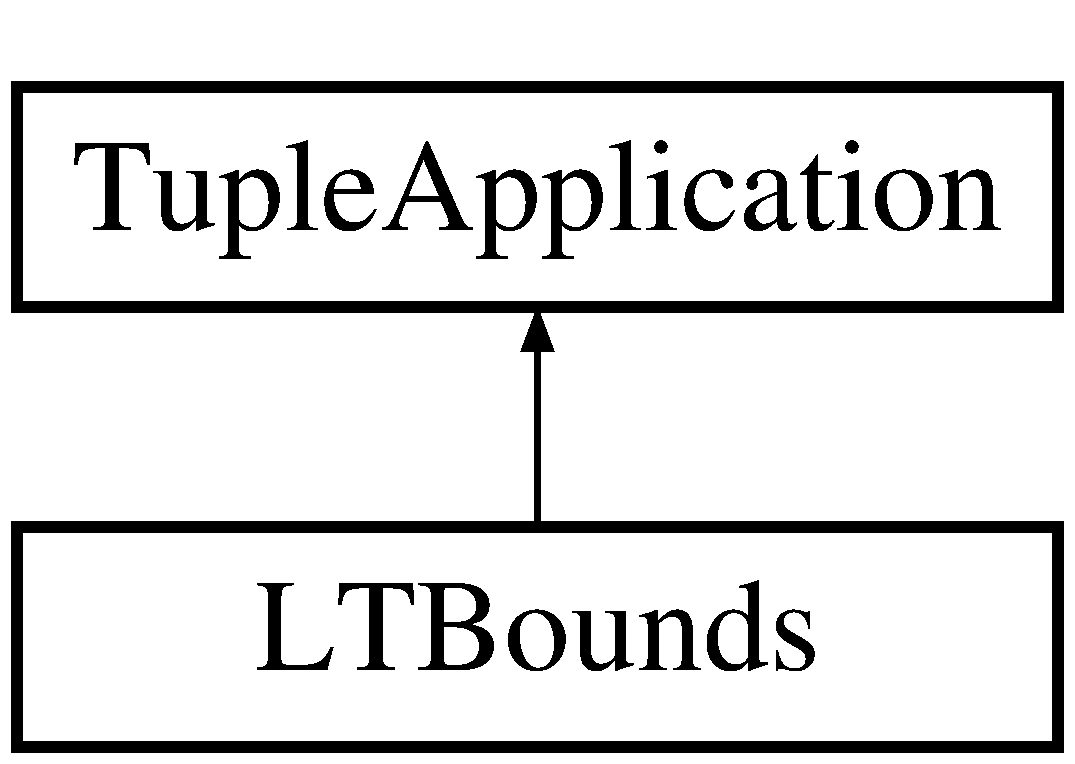
\includegraphics[height=2cm]{class_l_t_bounds}
\end{center}
\end{figure}
\subsection*{Protected Member Functions}
\begin{CompactItemize}
\item 
void \hyperlink{class_l_t_bounds_ac6861a60c9a42ec8fc71025b481c380}{consumeInput} ()
\item 
void \hyperlink{class_l_t_bounds_877b72b63e19fbb7114bae270fe20c53}{work} ()
\item 
void \hyperlink{class_l_t_bounds_028a451c099ee3377dc64a5a8ae9954f}{produceOutput} ()
\end{CompactItemize}
\subsection*{Static Protected Attributes}
\begin{CompactItemize}
\item 
static const char $\ast$ \hyperlink{class_l_t_bounds_80e32001ceca2a006abbf604c6359cef}{SYNCH\_\-LOCK} = \char`\"{}norm synch lock\char`\"{}
\item 
static const char $\ast$ \hyperlink{class_l_t_bounds_4b20608cc18141ad4427a373bb3f341c}{POINTS\_\-DONE} = \char`\"{}norm points reporting\char`\"{}
\item 
static const char $\ast$ \hyperlink{class_l_t_bounds_c8258b77f06e3eba82d3df7557c42829}{MIN\_\-POINT} = \char`\"{}norm minPoint\char`\"{}
\item 
static const char $\ast$ \hyperlink{class_l_t_bounds_8338863457650133e0aa18b5968d00fb}{MAX\_\-POINT} = \char`\"{}norm maxPoint\char`\"{}
\end{CompactItemize}


\subsection{Detailed Description}
Calculates the minimum/maximum point in the point cloud, so that the other points can be later normalized. Keeps those values in the tuple space so they can be used later. 

\subsection{Member Function Documentation}
\hypertarget{class_l_t_bounds_ac6861a60c9a42ec8fc71025b481c380}{
\index{LTBounds@{LTBounds}!consumeInput@{consumeInput}}
\index{consumeInput@{consumeInput}!LTBounds@{LTBounds}}
\subsubsection[{consumeInput}]{\setlength{\rightskip}{0pt plus 5cm}void LTBounds::consumeInput ()\hspace{0.3cm}{\tt  \mbox{[}protected, virtual\mbox{]}}}}
\label{class_l_t_bounds_ac6861a60c9a42ec8fc71025b481c380}


The consume input process is spawned once and should distribute tasks to the worker processes. 

Implements \hyperlink{class_tuple_application_e163c5a536de01c8b94b49528a17dab2}{TupleApplication}.\hypertarget{class_l_t_bounds_028a451c099ee3377dc64a5a8ae9954f}{
\index{LTBounds@{LTBounds}!produceOutput@{produceOutput}}
\index{produceOutput@{produceOutput}!LTBounds@{LTBounds}}
\subsubsection[{produceOutput}]{\setlength{\rightskip}{0pt plus 5cm}void LTBounds::produceOutput ()\hspace{0.3cm}{\tt  \mbox{[}protected, virtual\mbox{]}}}}
\label{class_l_t_bounds_028a451c099ee3377dc64a5a8ae9954f}


The output producer decides when the tuple application is finished; once this function returns, the tuple application is complete. 

Implements \hyperlink{class_tuple_application_8743dfcf17dedd52887c0b2ab170d8dc}{TupleApplication}.\hypertarget{class_l_t_bounds_877b72b63e19fbb7114bae270fe20c53}{
\index{LTBounds@{LTBounds}!work@{work}}
\index{work@{work}!LTBounds@{LTBounds}}
\subsubsection[{work}]{\setlength{\rightskip}{0pt plus 5cm}void LTBounds::work ()\hspace{0.3cm}{\tt  \mbox{[}protected, virtual\mbox{]}}}}
\label{class_l_t_bounds_877b72b63e19fbb7114bae270fe20c53}


Worker processes are created and killed after the output process has finished. 

Implements \hyperlink{class_tuple_application_ef6ae8bb1d697e4ed038b43320183c89}{TupleApplication}.

\subsection{Member Data Documentation}
\hypertarget{class_l_t_bounds_8338863457650133e0aa18b5968d00fb}{
\index{LTBounds@{LTBounds}!MAX\_\-POINT@{MAX\_\-POINT}}
\index{MAX\_\-POINT@{MAX\_\-POINT}!LTBounds@{LTBounds}}
\subsubsection[{MAX\_\-POINT}]{\setlength{\rightskip}{0pt plus 5cm}const char $\ast$ {\bf LTBounds::MAX\_\-POINT} = \char`\"{}norm maxPoint\char`\"{}\hspace{0.3cm}{\tt  \mbox{[}static, protected\mbox{]}}}}
\label{class_l_t_bounds_8338863457650133e0aa18b5968d00fb}


The largest point (in x and y) found \hypertarget{class_l_t_bounds_c8258b77f06e3eba82d3df7557c42829}{
\index{LTBounds@{LTBounds}!MIN\_\-POINT@{MIN\_\-POINT}}
\index{MIN\_\-POINT@{MIN\_\-POINT}!LTBounds@{LTBounds}}
\subsubsection[{MIN\_\-POINT}]{\setlength{\rightskip}{0pt plus 5cm}const char $\ast$ {\bf LTBounds::MIN\_\-POINT} = \char`\"{}norm minPoint\char`\"{}\hspace{0.3cm}{\tt  \mbox{[}static, protected\mbox{]}}}}
\label{class_l_t_bounds_c8258b77f06e3eba82d3df7557c42829}


The smallest point (in x and y) found \hypertarget{class_l_t_bounds_4b20608cc18141ad4427a373bb3f341c}{
\index{LTBounds@{LTBounds}!POINTS\_\-DONE@{POINTS\_\-DONE}}
\index{POINTS\_\-DONE@{POINTS\_\-DONE}!LTBounds@{LTBounds}}
\subsubsection[{POINTS\_\-DONE}]{\setlength{\rightskip}{0pt plus 5cm}const char $\ast$ {\bf LTBounds::POINTS\_\-DONE} = \char`\"{}norm points reporting\char`\"{}\hspace{0.3cm}{\tt  \mbox{[}static, protected\mbox{]}}}}
\label{class_l_t_bounds_4b20608cc18141ad4427a373bb3f341c}


Number of points that have been processed. \hypertarget{class_l_t_bounds_80e32001ceca2a006abbf604c6359cef}{
\index{LTBounds@{LTBounds}!SYNCH\_\-LOCK@{SYNCH\_\-LOCK}}
\index{SYNCH\_\-LOCK@{SYNCH\_\-LOCK}!LTBounds@{LTBounds}}
\subsubsection[{SYNCH\_\-LOCK}]{\setlength{\rightskip}{0pt plus 5cm}const char $\ast$ {\bf LTBounds::SYNCH\_\-LOCK} = \char`\"{}norm synch lock\char`\"{}\hspace{0.3cm}{\tt  \mbox{[}static, protected\mbox{]}}}}
\label{class_l_t_bounds_80e32001ceca2a006abbf604c6359cef}


Synchronization lock (critical section). 

The documentation for this class was generated from the following files:\begin{CompactItemize}
\item 
cowichan\_\-lt/src/\hyperlink{norm_8hpp}{norm.hpp}\item 
cowichan\_\-lt/src/\hyperlink{cowichan__lt_2src_2norm_8cpp}{norm.cpp}\end{CompactItemize}

\hypertarget{class_l_t_forward}{
\section{LTForward Class Reference}
\label{class_l_t_forward}\index{LTForward@{LTForward}}
}
{\tt \#include $<$gauss.hpp$>$}

Inheritance diagram for LTForward::\begin{figure}[H]
\begin{center}
\leavevmode
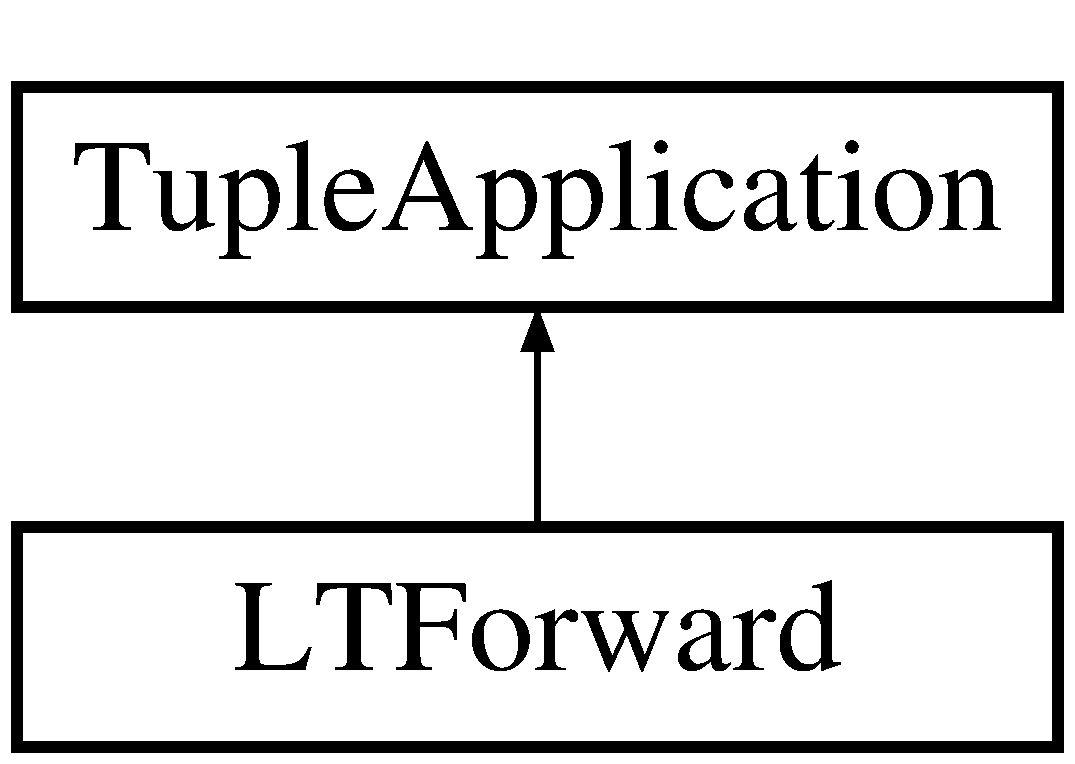
\includegraphics[height=2cm]{class_l_t_forward}
\end{center}
\end{figure}
\subsection*{Protected Member Functions}
\begin{CompactItemize}
\item 
void \hyperlink{class_l_t_forward_6f3bbdf720e1899b0df8a8f222727086}{consumeInput} ()
\item 
void \hyperlink{class_l_t_forward_d98aff7a063bf6e8542046c6f2c097fa}{work} ()
\item 
void \hyperlink{class_l_t_forward_56c27cd419407319f95afa4e7d43409a}{produceOutput} ()
\end{CompactItemize}
\subsection*{Static Protected Attributes}
\begin{CompactItemize}
\item 
static const char $\ast$ \hyperlink{class_l_t_forward_52da5e0079361dc8daf8c6a9a976c98d}{ROWS\_\-DONE} = \char`\"{}forward rows reporting\char`\"{}
\item 
static const char $\ast$ \hyperlink{class_l_t_forward_f638f80e205c1c7dc14766015d1247e6}{FORWARD\_\-DONE} = \char`\"{}forward done\char`\"{}
\item 
static const char $\ast$ \hyperlink{class_l_t_forward_e5706fd083624c202c274015935c865b}{REQUEST} = \char`\"{}forward request\char`\"{}
\item 
static const char $\ast$ \hyperlink{class_l_t_forward_79ab5e95abdc47acc8150941a17fb54a}{TARGET} = \char`\"{}gauss target\char`\"{}
\item 
static const char $\ast$ \hyperlink{class_l_t_forward_31820d362b40c3d15df139fde2f871f2}{MATRIX\_\-ROW} = \char`\"{}gauss matrix row\char`\"{}
\end{CompactItemize}


\subsection{Detailed Description}
Forward-elimination tuple application. Performs forward elimination on a square matrix in parallel. 

\subsection{Member Function Documentation}
\hypertarget{class_l_t_forward_6f3bbdf720e1899b0df8a8f222727086}{
\index{LTForward@{LTForward}!consumeInput@{consumeInput}}
\index{consumeInput@{consumeInput}!LTForward@{LTForward}}
\subsubsection[{consumeInput}]{\setlength{\rightskip}{0pt plus 5cm}void LTForward::consumeInput ()\hspace{0.3cm}{\tt  \mbox{[}protected, virtual\mbox{]}}}}
\label{class_l_t_forward_6f3bbdf720e1899b0df8a8f222727086}


The consume input process is spawned once and should distribute tasks to the worker processes. 

Implements \hyperlink{class_tuple_application_e163c5a536de01c8b94b49528a17dab2}{TupleApplication}.\hypertarget{class_l_t_forward_56c27cd419407319f95afa4e7d43409a}{
\index{LTForward@{LTForward}!produceOutput@{produceOutput}}
\index{produceOutput@{produceOutput}!LTForward@{LTForward}}
\subsubsection[{produceOutput}]{\setlength{\rightskip}{0pt plus 5cm}void LTForward::produceOutput ()\hspace{0.3cm}{\tt  \mbox{[}protected, virtual\mbox{]}}}}
\label{class_l_t_forward_56c27cd419407319f95afa4e7d43409a}


The output producer decides when the tuple application is finished; once this function returns, the tuple application is complete. 

Implements \hyperlink{class_tuple_application_8743dfcf17dedd52887c0b2ab170d8dc}{TupleApplication}.\hypertarget{class_l_t_forward_d98aff7a063bf6e8542046c6f2c097fa}{
\index{LTForward@{LTForward}!work@{work}}
\index{work@{work}!LTForward@{LTForward}}
\subsubsection[{work}]{\setlength{\rightskip}{0pt plus 5cm}void LTForward::work ()\hspace{0.3cm}{\tt  \mbox{[}protected, virtual\mbox{]}}}}
\label{class_l_t_forward_d98aff7a063bf6e8542046c6f2c097fa}


Worker processes are created and killed after the output process has finished. 

Implements \hyperlink{class_tuple_application_ef6ae8bb1d697e4ed038b43320183c89}{TupleApplication}.

\subsection{Member Data Documentation}
\hypertarget{class_l_t_forward_f638f80e205c1c7dc14766015d1247e6}{
\index{LTForward@{LTForward}!FORWARD\_\-DONE@{FORWARD\_\-DONE}}
\index{FORWARD\_\-DONE@{FORWARD\_\-DONE}!LTForward@{LTForward}}
\subsubsection[{FORWARD\_\-DONE}]{\setlength{\rightskip}{0pt plus 5cm}const char $\ast$ {\bf LTForward::FORWARD\_\-DONE} = \char`\"{}forward done\char`\"{}\hspace{0.3cm}{\tt  \mbox{[}static, protected\mbox{]}}}}
\label{class_l_t_forward_f638f80e205c1c7dc14766015d1247e6}


Is forward-elimination complete? \hypertarget{class_l_t_forward_31820d362b40c3d15df139fde2f871f2}{
\index{LTForward@{LTForward}!MATRIX\_\-ROW@{MATRIX\_\-ROW}}
\index{MATRIX\_\-ROW@{MATRIX\_\-ROW}!LTForward@{LTForward}}
\subsubsection[{MATRIX\_\-ROW}]{\setlength{\rightskip}{0pt plus 5cm}const char $\ast$ {\bf LTForward::MATRIX\_\-ROW} = \char`\"{}gauss matrix row\char`\"{}\hspace{0.3cm}{\tt  \mbox{[}static, protected\mbox{]}}}}
\label{class_l_t_forward_31820d362b40c3d15df139fde2f871f2}


One of the matrix rows, stored in the tuple space. \hypertarget{class_l_t_forward_e5706fd083624c202c274015935c865b}{
\index{LTForward@{LTForward}!REQUEST@{REQUEST}}
\index{REQUEST@{REQUEST}!LTForward@{LTForward}}
\subsubsection[{REQUEST}]{\setlength{\rightskip}{0pt plus 5cm}const char $\ast$ {\bf LTForward::REQUEST} = \char`\"{}forward request\char`\"{}\hspace{0.3cm}{\tt  \mbox{[}static, protected\mbox{]}}}}
\label{class_l_t_forward_e5706fd083624c202c274015935c865b}


A matrix row computation request. \hypertarget{class_l_t_forward_52da5e0079361dc8daf8c6a9a976c98d}{
\index{LTForward@{LTForward}!ROWS\_\-DONE@{ROWS\_\-DONE}}
\index{ROWS\_\-DONE@{ROWS\_\-DONE}!LTForward@{LTForward}}
\subsubsection[{ROWS\_\-DONE}]{\setlength{\rightskip}{0pt plus 5cm}const char $\ast$ {\bf LTForward::ROWS\_\-DONE} = \char`\"{}forward rows reporting\char`\"{}\hspace{0.3cm}{\tt  \mbox{[}static, protected\mbox{]}}}}
\label{class_l_t_forward_52da5e0079361dc8daf8c6a9a976c98d}


Number of rows computed. \hypertarget{class_l_t_forward_79ab5e95abdc47acc8150941a17fb54a}{
\index{LTForward@{LTForward}!TARGET@{TARGET}}
\index{TARGET@{TARGET}!LTForward@{LTForward}}
\subsubsection[{TARGET}]{\setlength{\rightskip}{0pt plus 5cm}const char $\ast$ {\bf LTForward::TARGET} = \char`\"{}gauss target\char`\"{}\hspace{0.3cm}{\tt  \mbox{[}static, protected\mbox{]}}}}
\label{class_l_t_forward_79ab5e95abdc47acc8150941a17fb54a}


The target vector stored in the tuple space. 

The documentation for this class was generated from the following files:\begin{CompactItemize}
\item 
cowichan\_\-lt/src/\hyperlink{gauss_8hpp}{gauss.hpp}\item 
cowichan\_\-lt/src/\hyperlink{cowichan__lt_2src_2gauss_8cpp}{gauss.cpp}\end{CompactItemize}

\hypertarget{class_l_t_frequency}{
\section{LTFrequency Class Reference}
\label{class_l_t_frequency}\index{LTFrequency@{LTFrequency}}
}
{\tt \#include $<$thresh.hpp$>$}

Inheritance diagram for LTFrequency::\begin{figure}[H]
\begin{center}
\leavevmode
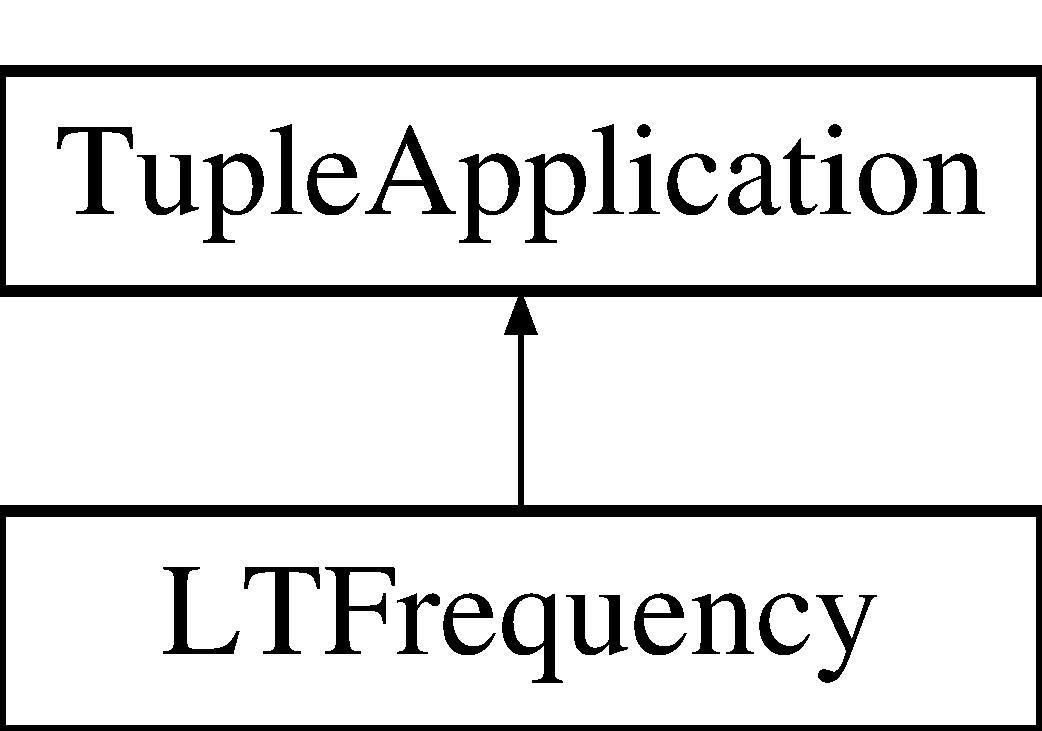
\includegraphics[height=2cm]{class_l_t_frequency}
\end{center}
\end{figure}
\subsection*{Protected Member Functions}
\begin{CompactItemize}
\item 
void \hyperlink{class_l_t_frequency_4ac4fa1a348246caf0d34506fcd09a64}{consumeInput} ()
\item 
void \hyperlink{class_l_t_frequency_7c47cf36b228505f79225a3fe8a00f01}{work} ()
\item 
void \hyperlink{class_l_t_frequency_e80cd869c8935cb7fe553c6ad27e861b}{produceOutput} ()
\end{CompactItemize}
\subsection*{Static Protected Attributes}
\begin{CompactItemize}
\item 
static const char $\ast$ \hyperlink{class_l_t_frequency_805150bf6fcc824bac1fcbb14914ecd4}{SYNCH\_\-LOCK} = \char`\"{}thresh synch lock\char`\"{}
\item 
static const char $\ast$ \hyperlink{class_l_t_frequency_db43dba3f48655d75150da76ff2a6a88}{ROWS\_\-DONE} = \char`\"{}thresh rows reporting\char`\"{}
\item 
static const char $\ast$ \hyperlink{class_l_t_frequency_f2db2bc6c1837dff0fa90a88a2290d62}{REQUEST} = \char`\"{}freq request\char`\"{}
\item 
static const char $\ast$ \hyperlink{class_l_t_frequency_731ba0c5b44e4ffa55496bceb2bd6578}{POINT} = \char`\"{}thresh point\char`\"{}
\end{CompactItemize}


\subsection{Detailed Description}
Counts the frequency of different values in a matrix; figures out the breaking point so that a certain percentage lay under the mark. 

\subsection{Member Function Documentation}
\hypertarget{class_l_t_frequency_4ac4fa1a348246caf0d34506fcd09a64}{
\index{LTFrequency@{LTFrequency}!consumeInput@{consumeInput}}
\index{consumeInput@{consumeInput}!LTFrequency@{LTFrequency}}
\subsubsection[{consumeInput}]{\setlength{\rightskip}{0pt plus 5cm}void LTFrequency::consumeInput ()\hspace{0.3cm}{\tt  \mbox{[}protected, virtual\mbox{]}}}}
\label{class_l_t_frequency_4ac4fa1a348246caf0d34506fcd09a64}


The consume input process is spawned once and should distribute tasks to the worker processes. 

Implements \hyperlink{class_tuple_application_e163c5a536de01c8b94b49528a17dab2}{TupleApplication}.\hypertarget{class_l_t_frequency_e80cd869c8935cb7fe553c6ad27e861b}{
\index{LTFrequency@{LTFrequency}!produceOutput@{produceOutput}}
\index{produceOutput@{produceOutput}!LTFrequency@{LTFrequency}}
\subsubsection[{produceOutput}]{\setlength{\rightskip}{0pt plus 5cm}void LTFrequency::produceOutput ()\hspace{0.3cm}{\tt  \mbox{[}protected, virtual\mbox{]}}}}
\label{class_l_t_frequency_e80cd869c8935cb7fe553c6ad27e861b}


The output producer decides when the tuple application is finished; once this function returns, the tuple application is complete. 

Implements \hyperlink{class_tuple_application_8743dfcf17dedd52887c0b2ab170d8dc}{TupleApplication}.\hypertarget{class_l_t_frequency_7c47cf36b228505f79225a3fe8a00f01}{
\index{LTFrequency@{LTFrequency}!work@{work}}
\index{work@{work}!LTFrequency@{LTFrequency}}
\subsubsection[{work}]{\setlength{\rightskip}{0pt plus 5cm}void LTFrequency::work ()\hspace{0.3cm}{\tt  \mbox{[}protected, virtual\mbox{]}}}}
\label{class_l_t_frequency_7c47cf36b228505f79225a3fe8a00f01}


Worker processes are created and killed after the output process has finished. 

Implements \hyperlink{class_tuple_application_ef6ae8bb1d697e4ed038b43320183c89}{TupleApplication}.

\subsection{Member Data Documentation}
\hypertarget{class_l_t_frequency_731ba0c5b44e4ffa55496bceb2bd6578}{
\index{LTFrequency@{LTFrequency}!POINT@{POINT}}
\index{POINT@{POINT}!LTFrequency@{LTFrequency}}
\subsubsection[{POINT}]{\setlength{\rightskip}{0pt plus 5cm}const char $\ast$ {\bf LTFrequency::POINT} = \char`\"{}thresh point\char`\"{}\hspace{0.3cm}{\tt  \mbox{[}static, protected\mbox{]}}}}
\label{class_l_t_frequency_731ba0c5b44e4ffa55496bceb2bd6578}


The breaking-point for the thresholding process. \hypertarget{class_l_t_frequency_f2db2bc6c1837dff0fa90a88a2290d62}{
\index{LTFrequency@{LTFrequency}!REQUEST@{REQUEST}}
\index{REQUEST@{REQUEST}!LTFrequency@{LTFrequency}}
\subsubsection[{REQUEST}]{\setlength{\rightskip}{0pt plus 5cm}const char $\ast$ {\bf LTFrequency::REQUEST} = \char`\"{}freq request\char`\"{}\hspace{0.3cm}{\tt  \mbox{[}static, protected\mbox{]}}}}
\label{class_l_t_frequency_f2db2bc6c1837dff0fa90a88a2290d62}


A request to compute a row. \hypertarget{class_l_t_frequency_db43dba3f48655d75150da76ff2a6a88}{
\index{LTFrequency@{LTFrequency}!ROWS\_\-DONE@{ROWS\_\-DONE}}
\index{ROWS\_\-DONE@{ROWS\_\-DONE}!LTFrequency@{LTFrequency}}
\subsubsection[{ROWS\_\-DONE}]{\setlength{\rightskip}{0pt plus 5cm}const char $\ast$ {\bf LTFrequency::ROWS\_\-DONE} = \char`\"{}thresh rows reporting\char`\"{}\hspace{0.3cm}{\tt  \mbox{[}static, protected\mbox{]}}}}
\label{class_l_t_frequency_db43dba3f48655d75150da76ff2a6a88}


Number of rows computed for. \hypertarget{class_l_t_frequency_805150bf6fcc824bac1fcbb14914ecd4}{
\index{LTFrequency@{LTFrequency}!SYNCH\_\-LOCK@{SYNCH\_\-LOCK}}
\index{SYNCH\_\-LOCK@{SYNCH\_\-LOCK}!LTFrequency@{LTFrequency}}
\subsubsection[{SYNCH\_\-LOCK}]{\setlength{\rightskip}{0pt plus 5cm}const char $\ast$ {\bf LTFrequency::SYNCH\_\-LOCK} = \char`\"{}thresh synch lock\char`\"{}\hspace{0.3cm}{\tt  \mbox{[}static, protected\mbox{]}}}}
\label{class_l_t_frequency_805150bf6fcc824bac1fcbb14914ecd4}


Synchronization lock (critical section). 

The documentation for this class was generated from the following files:\begin{CompactItemize}
\item 
cowichan\_\-lt/src/\hyperlink{thresh_8hpp}{thresh.hpp}\item 
cowichan\_\-lt/src/\hyperlink{cowichan__lt_2src_2thresh_8cpp}{thresh.cpp}\end{CompactItemize}

\hypertarget{class_l_t_half}{
\section{LTHalf Class Reference}
\label{class_l_t_half}\index{LTHalf@{LTHalf}}
}
{\tt \#include $<$half.hpp$>$}

Inheritance diagram for LTHalf::\begin{figure}[H]
\begin{center}
\leavevmode
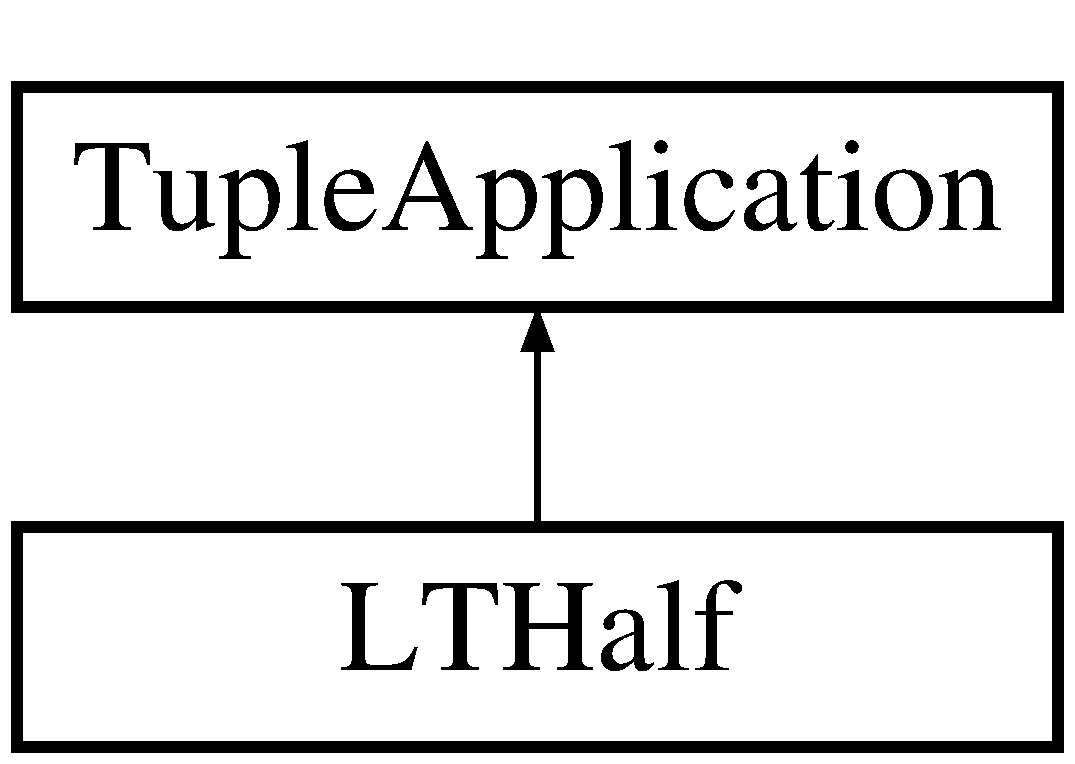
\includegraphics[height=2cm]{class_l_t_half}
\end{center}
\end{figure}
\subsection*{Protected Member Functions}
\begin{CompactItemize}
\item 
void \hyperlink{class_l_t_half_fc07035f40f22a3f827504b13e8f99c9}{consumeInput} ()
\item 
void \hyperlink{class_l_t_half_e60dd430fb782498837492c0331e0dea}{work} ()
\item 
void \hyperlink{class_l_t_half_bf36d89af87f94ff2aaff36338717f37}{produceOutput} ()
\end{CompactItemize}
\subsection*{Static Protected Attributes}
\begin{CompactItemize}
\item 
static const char $\ast$ \hyperlink{class_l_t_half_b5b706c81754d3d74f5ed82aa304d518}{REQUEST} = \char`\"{}half request\char`\"{}
\item 
static const char $\ast$ \hyperlink{class_l_t_half_2475f33ea01053a45cc88cbe207f3bd8}{DONE} = \char`\"{}half done\char`\"{}
\end{CompactItemize}


\subsection{Detailed Description}
Performs the halving shuffle on an input matrix. Generates an output matrix using LinuxTuples. 

\subsection{Member Function Documentation}
\hypertarget{class_l_t_half_fc07035f40f22a3f827504b13e8f99c9}{
\index{LTHalf@{LTHalf}!consumeInput@{consumeInput}}
\index{consumeInput@{consumeInput}!LTHalf@{LTHalf}}
\subsubsection[{consumeInput}]{\setlength{\rightskip}{0pt plus 5cm}void LTHalf::consumeInput ()\hspace{0.3cm}{\tt  \mbox{[}protected, virtual\mbox{]}}}}
\label{class_l_t_half_fc07035f40f22a3f827504b13e8f99c9}


The consume input process is spawned once and should distribute tasks to the worker processes. 

Implements \hyperlink{class_tuple_application_e163c5a536de01c8b94b49528a17dab2}{TupleApplication}.\hypertarget{class_l_t_half_bf36d89af87f94ff2aaff36338717f37}{
\index{LTHalf@{LTHalf}!produceOutput@{produceOutput}}
\index{produceOutput@{produceOutput}!LTHalf@{LTHalf}}
\subsubsection[{produceOutput}]{\setlength{\rightskip}{0pt plus 5cm}void LTHalf::produceOutput ()\hspace{0.3cm}{\tt  \mbox{[}protected, virtual\mbox{]}}}}
\label{class_l_t_half_bf36d89af87f94ff2aaff36338717f37}


The output producer decides when the tuple application is finished; once this function returns, the tuple application is complete. 

Implements \hyperlink{class_tuple_application_8743dfcf17dedd52887c0b2ab170d8dc}{TupleApplication}.\hypertarget{class_l_t_half_e60dd430fb782498837492c0331e0dea}{
\index{LTHalf@{LTHalf}!work@{work}}
\index{work@{work}!LTHalf@{LTHalf}}
\subsubsection[{work}]{\setlength{\rightskip}{0pt plus 5cm}void LTHalf::work ()\hspace{0.3cm}{\tt  \mbox{[}protected, virtual\mbox{]}}}}
\label{class_l_t_half_e60dd430fb782498837492c0331e0dea}


Worker processes are created and killed after the output process has finished. 

Implements \hyperlink{class_tuple_application_ef6ae8bb1d697e4ed038b43320183c89}{TupleApplication}.

\subsection{Member Data Documentation}
\hypertarget{class_l_t_half_2475f33ea01053a45cc88cbe207f3bd8}{
\index{LTHalf@{LTHalf}!DONE@{DONE}}
\index{DONE@{DONE}!LTHalf@{LTHalf}}
\subsubsection[{DONE}]{\setlength{\rightskip}{0pt plus 5cm}const char $\ast$ {\bf LTHalf::DONE} = \char`\"{}half done\char`\"{}\hspace{0.3cm}{\tt  \mbox{[}static, protected\mbox{]}}}}
\label{class_l_t_half_2475f33ea01053a45cc88cbe207f3bd8}


Done with the halving shuffle. \hypertarget{class_l_t_half_b5b706c81754d3d74f5ed82aa304d518}{
\index{LTHalf@{LTHalf}!REQUEST@{REQUEST}}
\index{REQUEST@{REQUEST}!LTHalf@{LTHalf}}
\subsubsection[{REQUEST}]{\setlength{\rightskip}{0pt plus 5cm}const char $\ast$ {\bf LTHalf::REQUEST} = \char`\"{}half request\char`\"{}\hspace{0.3cm}{\tt  \mbox{[}static, protected\mbox{]}}}}
\label{class_l_t_half_b5b706c81754d3d74f5ed82aa304d518}


A request to perform computation on a row of the matrix. 

The documentation for this class was generated from the following files:\begin{CompactItemize}
\item 
cowichan\_\-lt/src/\hyperlink{half_8hpp}{half.hpp}\item 
cowichan\_\-lt/src/\hyperlink{cowichan__lt_2src_2half_8cpp}{half.cpp}\end{CompactItemize}

\hypertarget{class_l_t_hull}{
\section{LTHull Class Reference}
\label{class_l_t_hull}\index{LTHull@{LTHull}}
}
{\tt \#include $<$hull.hpp$>$}

Inheritance diagram for LTHull::\begin{figure}[H]
\begin{center}
\leavevmode
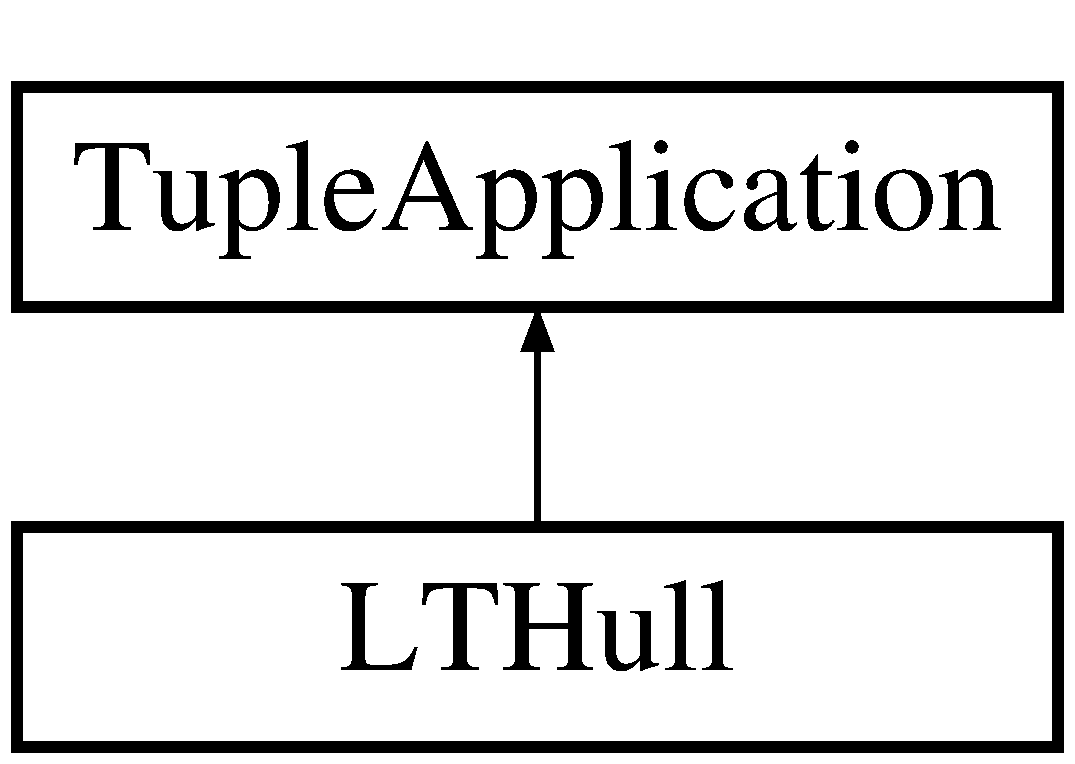
\includegraphics[height=2cm]{class_l_t_hull}
\end{center}
\end{figure}
\subsection*{Public Member Functions}
\begin{CompactItemize}
\item 
int \hyperlink{class_l_t_hull_73fa6d736d7caddc8ca45f1a50caded7}{getNumPoints} ()
\item 
\hyperlink{class_l_t_hull_b24a27789641c70a18de07cfec88f98a}{LTHull} (size\_\-t \hyperlink{class_l_t_hull_f0ebad39bb2bacecce2567da14aafb65}{numLeft})
\end{CompactItemize}
\subsection*{Static Public Attributes}
\begin{CompactItemize}
\item 
static const char $\ast$ \hyperlink{class_l_t_hull_07fb6b812c7950a5634f3d412baab762}{MASKED\_\-POINT} = \char`\"{}hull masked point\char`\"{}
\end{CompactItemize}
\subsection*{Protected Member Functions}
\begin{CompactItemize}
\item 
void \hyperlink{class_l_t_hull_e726f7fe6b16d8aa393045d4233a8447}{consumeInput} ()
\item 
void \hyperlink{class_l_t_hull_829b19b354bbe61d7cd5250819bd7b63}{work} ()
\item 
void \hyperlink{class_l_t_hull_14a3bf005173aa79d0c7259579229f12}{produceOutput} ()
\item 
void \hyperlink{class_l_t_hull_e18239f0a1a7f6504bc958b68a9b21fe}{split} (const \hyperlink{cowichan_8hpp_5b04577d5d21124855deaad298595371}{index\_\-t} p1, const \hyperlink{cowichan_8hpp_5b04577d5d21124855deaad298595371}{index\_\-t} p2, \hyperlink{cowichan_8hpp_5b04577d5d21124855deaad298595371}{index\_\-t} $\ast$order)
\item 
void \hyperlink{class_l_t_hull_9ba0913fac23bcf3fb42cc6bb212837f}{computeCross} (\hyperlink{cowichan_8hpp_5b04577d5d21124855deaad298595371}{index\_\-t} p1, \hyperlink{cowichan_8hpp_5b04577d5d21124855deaad298595371}{index\_\-t} p2, \hyperlink{cowichan_8hpp_5b04577d5d21124855deaad298595371}{index\_\-t} $\ast$maxPoint, \hyperlink{cowichan_8hpp_4d521b2c54a1f6312cc8fa04827eaf98}{real} $\ast$maxCross)
\item 
void \hyperlink{class_l_t_hull_0e932559e27a7cef73b76c22243e6c47}{computeMinMax} (\hyperlink{cowichan_8hpp_5b04577d5d21124855deaad298595371}{index\_\-t} $\ast$minPoint, \hyperlink{cowichan_8hpp_5b04577d5d21124855deaad298595371}{index\_\-t} $\ast$maxPoint)
\item 
void \hyperlink{class_l_t_hull_8f08515a49e5faf2d3808a623160767c}{serviceMinMaxRequest} (tuple $\ast$gotten)
\item 
void \hyperlink{class_l_t_hull_b803340b9529f56397ef7de752ad10cd}{serviceCrossRequest} (tuple $\ast$gotten)
\item 
bool \hyperlink{class_l_t_hull_b257bd2114c8726084351c4d1722cca1}{isMasked} (\hyperlink{cowichan_8hpp_5b04577d5d21124855deaad298595371}{index\_\-t} position)
\item 
void \hyperlink{class_l_t_hull_dc8df756ca767aef32450342c61d20e4}{mask} (\hyperlink{cowichan_8hpp_5b04577d5d21124855deaad298595371}{index\_\-t} position)
\end{CompactItemize}
\subsection*{Protected Attributes}
\begin{CompactItemize}
\item 
size\_\-t \hyperlink{class_l_t_hull_f0ebad39bb2bacecce2567da14aafb65}{numLeft}
\end{CompactItemize}
\subsection*{Static Protected Attributes}
\begin{CompactItemize}
\item 
static const char $\ast$ \hyperlink{class_l_t_hull_8ae87eb50cafb7fb26c3fe9fa33d8b1a}{REQUEST} = \char`\"{}hull request\char`\"{}
\item 
static const char $\ast$ \hyperlink{class_l_t_hull_4ac83a42baf632e37b12c27f3a8b9dae}{REQUEST\_\-MINMAX} = \char`\"{}hull request min/max\char`\"{}
\item 
static const char $\ast$ \hyperlink{class_l_t_hull_cb0b6736668d6ca4a71d69a739b3da9c}{REQUEST\_\-CROSS} = \char`\"{}hull request cross-product\char`\"{}
\item 
static const char $\ast$ \hyperlink{class_l_t_hull_0f5e7a0b036d18043f0b44c272a1f0f9}{SYNCH\_\-LOCK} = \char`\"{}hull synch lock\char`\"{}
\item 
static const char $\ast$ \hyperlink{class_l_t_hull_17e2355a00301575f9d862d562459c3c}{POINTS\_\-DONE} = \char`\"{}hull points reporting\char`\"{}
\item 
static const char $\ast$ \hyperlink{class_l_t_hull_b11b8a2223da908c7cbe796373090fe3}{MIN\_\-X\_\-POINT} = \char`\"{}hull minPoint\char`\"{}
\item 
static const char $\ast$ \hyperlink{class_l_t_hull_c73d8aee2d8caa920f085b5f097a518a}{MAX\_\-X\_\-POINT} = \char`\"{}hull maxPoint\char`\"{}
\item 
static const char $\ast$ \hyperlink{class_l_t_hull_c6b22ab53b74e4f651275b1cab27b3de}{MAX\_\-CROSS} = \char`\"{}hull max cross-product\char`\"{}
\item 
static const char $\ast$ \hyperlink{class_l_t_hull_7bcf7aface28e6ca262e98a9a8b8edf1}{MAX\_\-POINT} = \char`\"{}hull furthest point\char`\"{}
\item 
static const char $\ast$ \hyperlink{class_l_t_hull_e37ce27c8cd468ba8b535d05dfae6909}{HULL\_\-POINT} = \char`\"{}hull point\char`\"{}
\item 
static const char $\ast$ \hyperlink{class_l_t_hull_34e412ea0207b809b05c52be3d057a11}{NUM\_\-POINTS} = \char`\"{}hull \# of points in convex hull\char`\"{}
\item 
static const char $\ast$ \hyperlink{class_l_t_hull_4472a744a8960ba0848fffd9be4c5130}{FLAG\_\-OUTPUT} = \char`\"{}hull flag output\char`\"{}
\item 
static const char $\ast$ \hyperlink{class_l_t_hull_325452ed05b85f9ea185574d958635f9}{FINISHED\_\-MINMAX} = \char`\"{}hull finshed min/max\char`\"{}
\end{CompactItemize}


\subsection{Detailed Description}
Performs an iterative convex hull in tuple space. Iterative convex hull means that the output contains the convex hull of all points, followed by the convex hull of those points not on the first convex hull, followed by the convex hull of those points not on the first or second, etc. etc. until no points remain. Thus the iterative convex hull can be seen as a spiralling shape, or a permutation of the input points. 

\subsection{Constructor \& Destructor Documentation}
\hypertarget{class_l_t_hull_b24a27789641c70a18de07cfec88f98a}{
\index{LTHull@{LTHull}!LTHull@{LTHull}}
\index{LTHull@{LTHull}!LTHull@{LTHull}}
\subsubsection[{LTHull}]{\setlength{\rightskip}{0pt plus 5cm}LTHull::LTHull (size\_\-t {\em numLeft})}}
\label{class_l_t_hull_b24a27789641c70a18de07cfec88f98a}


Constructor. \begin{Desc}
\item[Parameters:]
\begin{description}
\item[{\em numLeft}]the number of points left unmasked in the input. \end{description}
\end{Desc}


\subsection{Member Function Documentation}
\hypertarget{class_l_t_hull_9ba0913fac23bcf3fb42cc6bb212837f}{
\index{LTHull@{LTHull}!computeCross@{computeCross}}
\index{computeCross@{computeCross}!LTHull@{LTHull}}
\subsubsection[{computeCross}]{\setlength{\rightskip}{0pt plus 5cm}void LTHull::computeCross ({\bf index\_\-t} {\em p1}, \/  {\bf index\_\-t} {\em p2}, \/  {\bf index\_\-t} $\ast$ {\em maxPoint}, \/  {\bf real} $\ast$ {\em maxCross})\hspace{0.3cm}{\tt  \mbox{[}protected\mbox{]}}}}
\label{class_l_t_hull_9ba0913fac23bcf3fb42cc6bb212837f}


Initiate a tuple-space cross-product over multiple points. \hypertarget{class_l_t_hull_0e932559e27a7cef73b76c22243e6c47}{
\index{LTHull@{LTHull}!computeMinMax@{computeMinMax}}
\index{computeMinMax@{computeMinMax}!LTHull@{LTHull}}
\subsubsection[{computeMinMax}]{\setlength{\rightskip}{0pt plus 5cm}void LTHull::computeMinMax ({\bf index\_\-t} $\ast$ {\em minPoint}, \/  {\bf index\_\-t} $\ast$ {\em maxPoint})\hspace{0.3cm}{\tt  \mbox{[}protected\mbox{]}}}}
\label{class_l_t_hull_0e932559e27a7cef73b76c22243e6c47}


Initiate a tuple-space min/max routine over multiple points. \hypertarget{class_l_t_hull_e726f7fe6b16d8aa393045d4233a8447}{
\index{LTHull@{LTHull}!consumeInput@{consumeInput}}
\index{consumeInput@{consumeInput}!LTHull@{LTHull}}
\subsubsection[{consumeInput}]{\setlength{\rightskip}{0pt plus 5cm}void LTHull::consumeInput ()\hspace{0.3cm}{\tt  \mbox{[}protected, virtual\mbox{]}}}}
\label{class_l_t_hull_e726f7fe6b16d8aa393045d4233a8447}


The consume input process is spawned once and should distribute tasks to the worker processes. 

Implements \hyperlink{class_tuple_application_e163c5a536de01c8b94b49528a17dab2}{TupleApplication}.\hypertarget{class_l_t_hull_73fa6d736d7caddc8ca45f1a50caded7}{
\index{LTHull@{LTHull}!getNumPoints@{getNumPoints}}
\index{getNumPoints@{getNumPoints}!LTHull@{LTHull}}
\subsubsection[{getNumPoints}]{\setlength{\rightskip}{0pt plus 5cm}int LTHull::getNumPoints ()}}
\label{class_l_t_hull_73fa6d736d7caddc8ca45f1a50caded7}


Returns the number of points in the convex hull. \hypertarget{class_l_t_hull_b257bd2114c8726084351c4d1722cca1}{
\index{LTHull@{LTHull}!isMasked@{isMasked}}
\index{isMasked@{isMasked}!LTHull@{LTHull}}
\subsubsection[{isMasked}]{\setlength{\rightskip}{0pt plus 5cm}bool LTHull::isMasked ({\bf index\_\-t} {\em position})\hspace{0.3cm}{\tt  \mbox{[}protected\mbox{]}}}}
\label{class_l_t_hull_b257bd2114c8726084351c4d1722cca1}


Is the given point \char`\"{}masked\char`\"{}, i.e., should we skip it? \begin{Desc}
\item[Parameters:]
\begin{description}
\item[{\em position}]the point to check. \end{description}
\end{Desc}
\begin{Desc}
\item[Returns:]true if the point is to be skipped, false otherwise. \end{Desc}
\hypertarget{class_l_t_hull_dc8df756ca767aef32450342c61d20e4}{
\index{LTHull@{LTHull}!mask@{mask}}
\index{mask@{mask}!LTHull@{LTHull}}
\subsubsection[{mask}]{\setlength{\rightskip}{0pt plus 5cm}void LTHull::mask ({\bf index\_\-t} {\em position})\hspace{0.3cm}{\tt  \mbox{[}protected\mbox{]}}}}
\label{class_l_t_hull_dc8df756ca767aef32450342c61d20e4}


Mask the given point (make sure we skip it next time we do a convex hull computation). \begin{Desc}
\item[Parameters:]
\begin{description}
\item[{\em position}]the point to mask. \end{description}
\end{Desc}
\hypertarget{class_l_t_hull_14a3bf005173aa79d0c7259579229f12}{
\index{LTHull@{LTHull}!produceOutput@{produceOutput}}
\index{produceOutput@{produceOutput}!LTHull@{LTHull}}
\subsubsection[{produceOutput}]{\setlength{\rightskip}{0pt plus 5cm}void LTHull::produceOutput ()\hspace{0.3cm}{\tt  \mbox{[}protected, virtual\mbox{]}}}}
\label{class_l_t_hull_14a3bf005173aa79d0c7259579229f12}


The output producer decides when the tuple application is finished; once this function returns, the tuple application is complete. 

Implements \hyperlink{class_tuple_application_8743dfcf17dedd52887c0b2ab170d8dc}{TupleApplication}.\hypertarget{class_l_t_hull_b803340b9529f56397ef7de752ad10cd}{
\index{LTHull@{LTHull}!serviceCrossRequest@{serviceCrossRequest}}
\index{serviceCrossRequest@{serviceCrossRequest}!LTHull@{LTHull}}
\subsubsection[{serviceCrossRequest}]{\setlength{\rightskip}{0pt plus 5cm}void LTHull::serviceCrossRequest (tuple $\ast$ {\em gotten})\hspace{0.3cm}{\tt  \mbox{[}protected\mbox{]}}}}
\label{class_l_t_hull_b803340b9529f56397ef7de752ad10cd}


Worker helper to server a cross-product request. \hypertarget{class_l_t_hull_8f08515a49e5faf2d3808a623160767c}{
\index{LTHull@{LTHull}!serviceMinMaxRequest@{serviceMinMaxRequest}}
\index{serviceMinMaxRequest@{serviceMinMaxRequest}!LTHull@{LTHull}}
\subsubsection[{serviceMinMaxRequest}]{\setlength{\rightskip}{0pt plus 5cm}void LTHull::serviceMinMaxRequest (tuple $\ast$ {\em gotten})\hspace{0.3cm}{\tt  \mbox{[}protected\mbox{]}}}}
\label{class_l_t_hull_8f08515a49e5faf2d3808a623160767c}


Worker helper to service a min/max request. \hypertarget{class_l_t_hull_e18239f0a1a7f6504bc958b68a9b21fe}{
\index{LTHull@{LTHull}!split@{split}}
\index{split@{split}!LTHull@{LTHull}}
\subsubsection[{split}]{\setlength{\rightskip}{0pt plus 5cm}void LTHull::split (const {\bf index\_\-t} {\em p1}, \/  const {\bf index\_\-t} {\em p2}, \/  {\bf index\_\-t} $\ast$ {\em order})\hspace{0.3cm}{\tt  \mbox{[}protected\mbox{]}}}}
\label{class_l_t_hull_e18239f0a1a7f6504bc958b68a9b21fe}


Analogous to split in other versions of quickhull. split again based on the furthest point from the line denoted by the two points given (p1 and p2).

Compute hull on one side of the splitting line. \begin{Desc}
\item[Parameters:]
\begin{description}
\item[{\em p1}]boundary point \#1. \item[{\em p2}]boundary point \#2. \item[{\em order}]the ordering number of the next hull point to emit. \end{description}
\end{Desc}
\hypertarget{class_l_t_hull_829b19b354bbe61d7cd5250819bd7b63}{
\index{LTHull@{LTHull}!work@{work}}
\index{work@{work}!LTHull@{LTHull}}
\subsubsection[{work}]{\setlength{\rightskip}{0pt plus 5cm}void LTHull::work ()\hspace{0.3cm}{\tt  \mbox{[}protected, virtual\mbox{]}}}}
\label{class_l_t_hull_829b19b354bbe61d7cd5250819bd7b63}


Worker processes are created and killed after the output process has finished. 

Implements \hyperlink{class_tuple_application_ef6ae8bb1d697e4ed038b43320183c89}{TupleApplication}.

\subsection{Member Data Documentation}
\hypertarget{class_l_t_hull_325452ed05b85f9ea185574d958635f9}{
\index{LTHull@{LTHull}!FINISHED\_\-MINMAX@{FINISHED\_\-MINMAX}}
\index{FINISHED\_\-MINMAX@{FINISHED\_\-MINMAX}!LTHull@{LTHull}}
\subsubsection[{FINISHED\_\-MINMAX}]{\setlength{\rightskip}{0pt plus 5cm}const char $\ast$ {\bf LTHull::FINISHED\_\-MINMAX} = \char`\"{}hull finshed min/max\char`\"{}\hspace{0.3cm}{\tt  \mbox{[}static, protected\mbox{]}}}}
\label{class_l_t_hull_325452ed05b85f9ea185574d958635f9}


The min-max process mandated has been finished. \hypertarget{class_l_t_hull_4472a744a8960ba0848fffd9be4c5130}{
\index{LTHull@{LTHull}!FLAG\_\-OUTPUT@{FLAG\_\-OUTPUT}}
\index{FLAG\_\-OUTPUT@{FLAG\_\-OUTPUT}!LTHull@{LTHull}}
\subsubsection[{FLAG\_\-OUTPUT}]{\setlength{\rightskip}{0pt plus 5cm}const char $\ast$ {\bf LTHull::FLAG\_\-OUTPUT} = \char`\"{}hull flag output\char`\"{}\hspace{0.3cm}{\tt  \mbox{[}static, protected\mbox{]}}}}
\label{class_l_t_hull_4472a744a8960ba0848fffd9be4c5130}


Should the output producer run now? \hypertarget{class_l_t_hull_e37ce27c8cd468ba8b535d05dfae6909}{
\index{LTHull@{LTHull}!HULL\_\-POINT@{HULL\_\-POINT}}
\index{HULL\_\-POINT@{HULL\_\-POINT}!LTHull@{LTHull}}
\subsubsection[{HULL\_\-POINT}]{\setlength{\rightskip}{0pt plus 5cm}const char $\ast$ {\bf LTHull::HULL\_\-POINT} = \char`\"{}hull point\char`\"{}\hspace{0.3cm}{\tt  \mbox{[}static, protected\mbox{]}}}}
\label{class_l_t_hull_e37ce27c8cd468ba8b535d05dfae6909}


A point on the hull, ordered. \hypertarget{class_l_t_hull_07fb6b812c7950a5634f3d412baab762}{
\index{LTHull@{LTHull}!MASKED\_\-POINT@{MASKED\_\-POINT}}
\index{MASKED\_\-POINT@{MASKED\_\-POINT}!LTHull@{LTHull}}
\subsubsection[{MASKED\_\-POINT}]{\setlength{\rightskip}{0pt plus 5cm}const char $\ast$ {\bf LTHull::MASKED\_\-POINT} = \char`\"{}hull masked point\char`\"{}\hspace{0.3cm}{\tt  \mbox{[}static\mbox{]}}}}
\label{class_l_t_hull_07fb6b812c7950a5634f3d412baab762}


The index of a point that is masked off (i.e. already selected) in the input. This is public so we can access it from \hyperlink{class_cowichan_linux_tuples_501f87594d62af261ff0b1954a60ddc4}{CowichanLinuxTuples::hull}(...). \hypertarget{class_l_t_hull_c6b22ab53b74e4f651275b1cab27b3de}{
\index{LTHull@{LTHull}!MAX\_\-CROSS@{MAX\_\-CROSS}}
\index{MAX\_\-CROSS@{MAX\_\-CROSS}!LTHull@{LTHull}}
\subsubsection[{MAX\_\-CROSS}]{\setlength{\rightskip}{0pt plus 5cm}const char $\ast$ {\bf LTHull::MAX\_\-CROSS} = \char`\"{}hull max cross-product\char`\"{}\hspace{0.3cm}{\tt  \mbox{[}static, protected\mbox{]}}}}
\label{class_l_t_hull_c6b22ab53b74e4f651275b1cab27b3de}


The cross product value of the \char`\"{}furthest\char`\"{} point. \hypertarget{class_l_t_hull_7bcf7aface28e6ca262e98a9a8b8edf1}{
\index{LTHull@{LTHull}!MAX\_\-POINT@{MAX\_\-POINT}}
\index{MAX\_\-POINT@{MAX\_\-POINT}!LTHull@{LTHull}}
\subsubsection[{MAX\_\-POINT}]{\setlength{\rightskip}{0pt plus 5cm}const char $\ast$ {\bf LTHull::MAX\_\-POINT} = \char`\"{}hull furthest point\char`\"{}\hspace{0.3cm}{\tt  \mbox{[}static, protected\mbox{]}}}}
\label{class_l_t_hull_7bcf7aface28e6ca262e98a9a8b8edf1}


The \char`\"{}furthest\char`\"{} point found. \hypertarget{class_l_t_hull_c73d8aee2d8caa920f085b5f097a518a}{
\index{LTHull@{LTHull}!MAX\_\-X\_\-POINT@{MAX\_\-X\_\-POINT}}
\index{MAX\_\-X\_\-POINT@{MAX\_\-X\_\-POINT}!LTHull@{LTHull}}
\subsubsection[{MAX\_\-X\_\-POINT}]{\setlength{\rightskip}{0pt plus 5cm}const char $\ast$ {\bf LTHull::MAX\_\-X\_\-POINT} = \char`\"{}hull maxPoint\char`\"{}\hspace{0.3cm}{\tt  \mbox{[}static, protected\mbox{]}}}}
\label{class_l_t_hull_c73d8aee2d8caa920f085b5f097a518a}


The point with highest x value, unmasked. \hypertarget{class_l_t_hull_b11b8a2223da908c7cbe796373090fe3}{
\index{LTHull@{LTHull}!MIN\_\-X\_\-POINT@{MIN\_\-X\_\-POINT}}
\index{MIN\_\-X\_\-POINT@{MIN\_\-X\_\-POINT}!LTHull@{LTHull}}
\subsubsection[{MIN\_\-X\_\-POINT}]{\setlength{\rightskip}{0pt plus 5cm}const char $\ast$ {\bf LTHull::MIN\_\-X\_\-POINT} = \char`\"{}hull minPoint\char`\"{}\hspace{0.3cm}{\tt  \mbox{[}static, protected\mbox{]}}}}
\label{class_l_t_hull_b11b8a2223da908c7cbe796373090fe3}


The point with lowest x value, unmasked. \hypertarget{class_l_t_hull_34e412ea0207b809b05c52be3d057a11}{
\index{LTHull@{LTHull}!NUM\_\-POINTS@{NUM\_\-POINTS}}
\index{NUM\_\-POINTS@{NUM\_\-POINTS}!LTHull@{LTHull}}
\subsubsection[{NUM\_\-POINTS}]{\setlength{\rightskip}{0pt plus 5cm}const char $\ast$ {\bf LTHull::NUM\_\-POINTS} = \char`\"{}hull \# of points in convex hull\char`\"{}\hspace{0.3cm}{\tt  \mbox{[}static, protected\mbox{]}}}}
\label{class_l_t_hull_34e412ea0207b809b05c52be3d057a11}


The number of points in this convex hull. \hypertarget{class_l_t_hull_f0ebad39bb2bacecce2567da14aafb65}{
\index{LTHull@{LTHull}!numLeft@{numLeft}}
\index{numLeft@{numLeft}!LTHull@{LTHull}}
\subsubsection[{numLeft}]{\setlength{\rightskip}{0pt plus 5cm}size\_\-t {\bf LTHull::numLeft}\hspace{0.3cm}{\tt  \mbox{[}protected\mbox{]}}}}
\label{class_l_t_hull_f0ebad39bb2bacecce2567da14aafb65}


The number of points left unmasked in the input. \hypertarget{class_l_t_hull_17e2355a00301575f9d862d562459c3c}{
\index{LTHull@{LTHull}!POINTS\_\-DONE@{POINTS\_\-DONE}}
\index{POINTS\_\-DONE@{POINTS\_\-DONE}!LTHull@{LTHull}}
\subsubsection[{POINTS\_\-DONE}]{\setlength{\rightskip}{0pt plus 5cm}const char $\ast$ {\bf LTHull::POINTS\_\-DONE} = \char`\"{}hull points reporting\char`\"{}\hspace{0.3cm}{\tt  \mbox{[}static, protected\mbox{]}}}}
\label{class_l_t_hull_17e2355a00301575f9d862d562459c3c}


The number of points that have been computed for. \hypertarget{class_l_t_hull_8ae87eb50cafb7fb26c3fe9fa33d8b1a}{
\index{LTHull@{LTHull}!REQUEST@{REQUEST}}
\index{REQUEST@{REQUEST}!LTHull@{LTHull}}
\subsubsection[{REQUEST}]{\setlength{\rightskip}{0pt plus 5cm}const char $\ast$ {\bf LTHull::REQUEST} = \char`\"{}hull request\char`\"{}\hspace{0.3cm}{\tt  \mbox{[}static, protected\mbox{]}}}}
\label{class_l_t_hull_8ae87eb50cafb7fb26c3fe9fa33d8b1a}


Generic request for work to be done. \hypertarget{class_l_t_hull_cb0b6736668d6ca4a71d69a739b3da9c}{
\index{LTHull@{LTHull}!REQUEST\_\-CROSS@{REQUEST\_\-CROSS}}
\index{REQUEST\_\-CROSS@{REQUEST\_\-CROSS}!LTHull@{LTHull}}
\subsubsection[{REQUEST\_\-CROSS}]{\setlength{\rightskip}{0pt plus 5cm}const char $\ast$ {\bf LTHull::REQUEST\_\-CROSS} = \char`\"{}hull request cross-product\char`\"{}\hspace{0.3cm}{\tt  \mbox{[}static, protected\mbox{]}}}}
\label{class_l_t_hull_cb0b6736668d6ca4a71d69a739b3da9c}


Specific work: cross-product request over a length of points. \hypertarget{class_l_t_hull_4ac83a42baf632e37b12c27f3a8b9dae}{
\index{LTHull@{LTHull}!REQUEST\_\-MINMAX@{REQUEST\_\-MINMAX}}
\index{REQUEST\_\-MINMAX@{REQUEST\_\-MINMAX}!LTHull@{LTHull}}
\subsubsection[{REQUEST\_\-MINMAX}]{\setlength{\rightskip}{0pt plus 5cm}const char $\ast$ {\bf LTHull::REQUEST\_\-MINMAX} = \char`\"{}hull request min/max\char`\"{}\hspace{0.3cm}{\tt  \mbox{[}static, protected\mbox{]}}}}
\label{class_l_t_hull_4ac83a42baf632e37b12c27f3a8b9dae}


Specific work: min-max request over a length of points. \hypertarget{class_l_t_hull_0f5e7a0b036d18043f0b44c272a1f0f9}{
\index{LTHull@{LTHull}!SYNCH\_\-LOCK@{SYNCH\_\-LOCK}}
\index{SYNCH\_\-LOCK@{SYNCH\_\-LOCK}!LTHull@{LTHull}}
\subsubsection[{SYNCH\_\-LOCK}]{\setlength{\rightskip}{0pt plus 5cm}const char $\ast$ {\bf LTHull::SYNCH\_\-LOCK} = \char`\"{}hull synch lock\char`\"{}\hspace{0.3cm}{\tt  \mbox{[}static, protected\mbox{]}}}}
\label{class_l_t_hull_0f5e7a0b036d18043f0b44c272a1f0f9}


Synchronization lock (critical section). 

The documentation for this class was generated from the following files:\begin{CompactItemize}
\item 
cowichan\_\-lt/src/\hyperlink{hull_8hpp}{hull.hpp}\item 
cowichan\_\-lt/src/\hyperlink{cowichan__lt_2src_2hull_8cpp}{hull.cpp}\end{CompactItemize}

\hypertarget{class_l_t_life}{
\section{LTLife Class Reference}
\label{class_l_t_life}\index{LTLife@{LTLife}}
}
{\tt \#include $<$life.hpp$>$}

Inheritance diagram for LTLife::\begin{figure}[H]
\begin{center}
\leavevmode
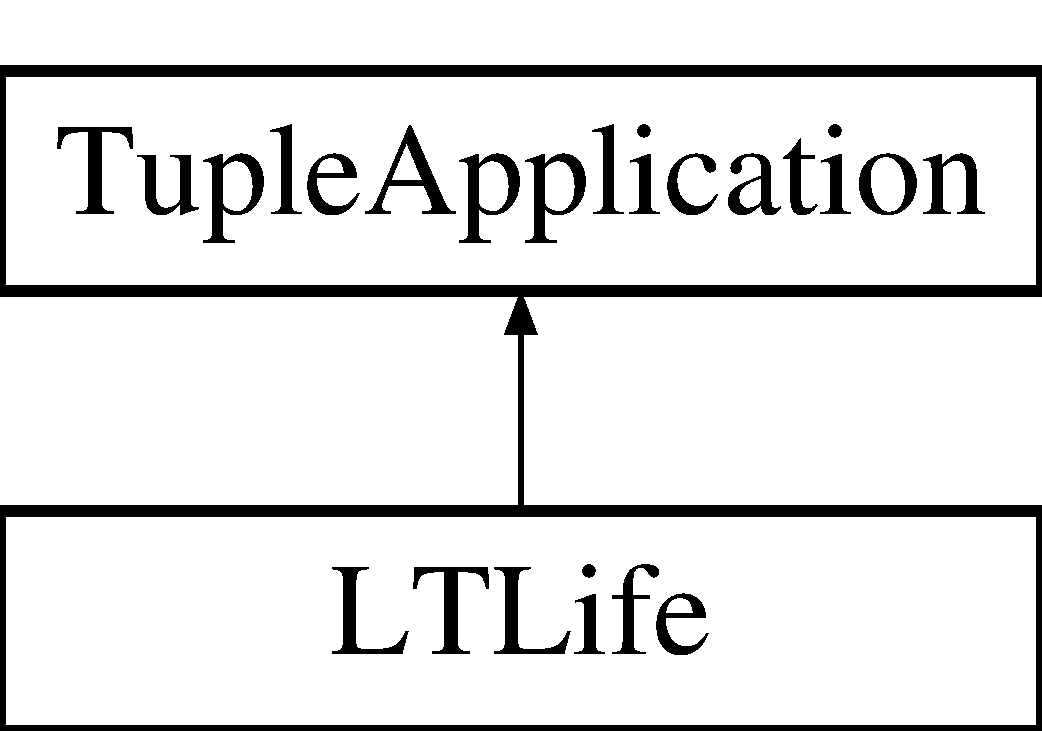
\includegraphics[height=2cm]{class_l_t_life}
\end{center}
\end{figure}
\subsection*{Protected Member Functions}
\begin{CompactItemize}
\item 
void \hyperlink{class_l_t_life_da0a691f9bf8bb055a4fe953dd6eb809}{consumeInput} ()
\item 
void \hyperlink{class_l_t_life_c0600864c1742c2a12e15992c539c2da}{work} ()
\item 
void \hyperlink{class_l_t_life_a0ac21131813f89a94c6ba7515e63c11}{produceOutput} ()
\item 
\hyperlink{cowichan_8hpp_5b04577d5d21124855deaad298595371}{index\_\-t} \hyperlink{class_l_t_life_c63c1d93bcffbd2415d23a189c46bce7}{sumNeighbours} (\hyperlink{cowichan_8hpp_5b04577d5d21124855deaad298595371}{index\_\-t} y, \hyperlink{cowichan_8hpp_5b04577d5d21124855deaad298595371}{index\_\-t} x)
\end{CompactItemize}


\subsection{Detailed Description}
Cellular automata done in LinuxTuples. 

\subsection{Member Function Documentation}
\hypertarget{class_l_t_life_da0a691f9bf8bb055a4fe953dd6eb809}{
\index{LTLife@{LTLife}!consumeInput@{consumeInput}}
\index{consumeInput@{consumeInput}!LTLife@{LTLife}}
\subsubsection[{consumeInput}]{\setlength{\rightskip}{0pt plus 5cm}void LTLife::consumeInput ()\hspace{0.3cm}{\tt  \mbox{[}protected, virtual\mbox{]}}}}
\label{class_l_t_life_da0a691f9bf8bb055a4fe953dd6eb809}


The consume input process is spawned once and should distribute tasks to the worker processes. 

Implements \hyperlink{class_tuple_application_e163c5a536de01c8b94b49528a17dab2}{TupleApplication}.\hypertarget{class_l_t_life_a0ac21131813f89a94c6ba7515e63c11}{
\index{LTLife@{LTLife}!produceOutput@{produceOutput}}
\index{produceOutput@{produceOutput}!LTLife@{LTLife}}
\subsubsection[{produceOutput}]{\setlength{\rightskip}{0pt plus 5cm}void LTLife::produceOutput ()\hspace{0.3cm}{\tt  \mbox{[}protected, virtual\mbox{]}}}}
\label{class_l_t_life_a0ac21131813f89a94c6ba7515e63c11}


The output producer decides when the tuple application is finished; once this function returns, the tuple application is complete. 

Implements \hyperlink{class_tuple_application_8743dfcf17dedd52887c0b2ab170d8dc}{TupleApplication}.\hypertarget{class_l_t_life_c63c1d93bcffbd2415d23a189c46bce7}{
\index{LTLife@{LTLife}!sumNeighbours@{sumNeighbours}}
\index{sumNeighbours@{sumNeighbours}!LTLife@{LTLife}}
\subsubsection[{sumNeighbours}]{\setlength{\rightskip}{0pt plus 5cm}{\bf index\_\-t} LTLife::sumNeighbours ({\bf index\_\-t} {\em y}, \/  {\bf index\_\-t} {\em x})\hspace{0.3cm}{\tt  \mbox{[}protected\mbox{]}}}}
\label{class_l_t_life_c63c1d93bcffbd2415d23a189c46bce7}


Calculate number of peers. \hypertarget{class_l_t_life_c0600864c1742c2a12e15992c539c2da}{
\index{LTLife@{LTLife}!work@{work}}
\index{work@{work}!LTLife@{LTLife}}
\subsubsection[{work}]{\setlength{\rightskip}{0pt plus 5cm}void LTLife::work ()\hspace{0.3cm}{\tt  \mbox{[}protected, virtual\mbox{]}}}}
\label{class_l_t_life_c0600864c1742c2a12e15992c539c2da}


Worker processes are created and killed after the output process has finished. 

Implements \hyperlink{class_tuple_application_ef6ae8bb1d697e4ed038b43320183c89}{TupleApplication}.

The documentation for this class was generated from the following files:\begin{CompactItemize}
\item 
cowichan\_\-lt/src/\hyperlink{life_8hpp}{life.hpp}\item 
cowichan\_\-lt/src/\hyperlink{cowichan__lt_2src_2life_8cpp}{life.cpp}\end{CompactItemize}

\hypertarget{class_l_t_mandel}{
\section{LTMandel Class Reference}
\label{class_l_t_mandel}\index{LTMandel@{LTMandel}}
}
{\tt \#include $<$mandel.hpp$>$}

Inheritance diagram for LTMandel::\begin{figure}[H]
\begin{center}
\leavevmode
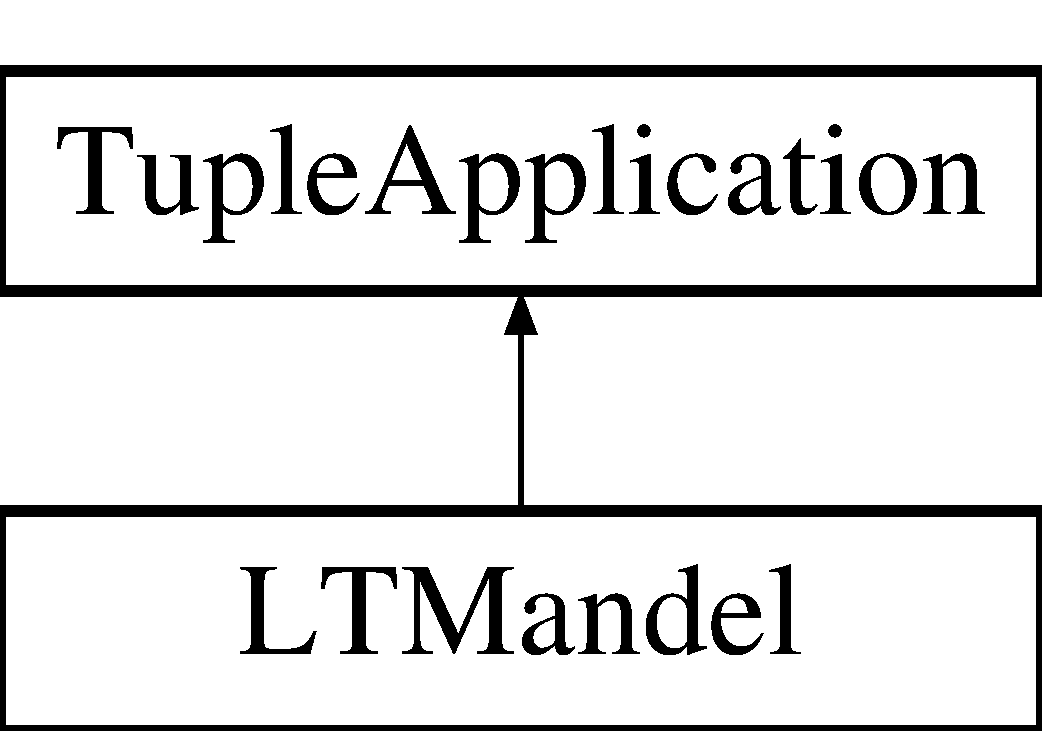
\includegraphics[height=2cm]{class_l_t_mandel}
\end{center}
\end{figure}
\subsection*{Protected Member Functions}
\begin{CompactItemize}
\item 
void \hyperlink{class_l_t_mandel_15fb4ee93967f8717db22056f666f723}{consumeInput} ()
\item 
void \hyperlink{class_l_t_mandel_5ea4d32e6d16f64148bddbb940d732da}{work} ()
\item 
void \hyperlink{class_l_t_mandel_31cacf747914e03e6a87bb9af7dff67e}{produceOutput} ()
\item 
int \hyperlink{class_l_t_mandel_c7b6459667c66226cc5745309493cdef}{mandelCalc} (\hyperlink{cowichan_8hpp_4d521b2c54a1f6312cc8fa04827eaf98}{real} x, \hyperlink{cowichan_8hpp_4d521b2c54a1f6312cc8fa04827eaf98}{real} y)
\end{CompactItemize}


\subsection{Detailed Description}
Calculates the mandelbrot set on a row-by-row basis. Uses LinuxTuples to do the heavy lifting. 

\subsection{Member Function Documentation}
\hypertarget{class_l_t_mandel_15fb4ee93967f8717db22056f666f723}{
\index{LTMandel@{LTMandel}!consumeInput@{consumeInput}}
\index{consumeInput@{consumeInput}!LTMandel@{LTMandel}}
\subsubsection[{consumeInput}]{\setlength{\rightskip}{0pt plus 5cm}void LTMandel::consumeInput ()\hspace{0.3cm}{\tt  \mbox{[}protected, virtual\mbox{]}}}}
\label{class_l_t_mandel_15fb4ee93967f8717db22056f666f723}


The consume input process is spawned once and should distribute tasks to the worker processes. 

Implements \hyperlink{class_tuple_application_e163c5a536de01c8b94b49528a17dab2}{TupleApplication}.\hypertarget{class_l_t_mandel_c7b6459667c66226cc5745309493cdef}{
\index{LTMandel@{LTMandel}!mandelCalc@{mandelCalc}}
\index{mandelCalc@{mandelCalc}!LTMandel@{LTMandel}}
\subsubsection[{mandelCalc}]{\setlength{\rightskip}{0pt plus 5cm}int LTMandel::mandelCalc ({\bf real} {\em x}, \/  {\bf real} {\em y})\hspace{0.3cm}{\tt  \mbox{[}protected\mbox{]}}}}
\label{class_l_t_mandel_c7b6459667c66226cc5745309493cdef}


Computes a part of the mandelbrot set. \begin{Desc}
\item[Parameters:]
\begin{description}
\item[{\em x}]x co-ordinate to compute for. \item[{\em y}]y co-ordinate to compute for. \end{description}
\end{Desc}
\begin{Desc}
\item[Returns:]the computed value at (x,y) on the mandelbrot set. \end{Desc}
\hypertarget{class_l_t_mandel_31cacf747914e03e6a87bb9af7dff67e}{
\index{LTMandel@{LTMandel}!produceOutput@{produceOutput}}
\index{produceOutput@{produceOutput}!LTMandel@{LTMandel}}
\subsubsection[{produceOutput}]{\setlength{\rightskip}{0pt plus 5cm}void LTMandel::produceOutput ()\hspace{0.3cm}{\tt  \mbox{[}protected, virtual\mbox{]}}}}
\label{class_l_t_mandel_31cacf747914e03e6a87bb9af7dff67e}


The output producer decides when the tuple application is finished; once this function returns, the tuple application is complete. 

Implements \hyperlink{class_tuple_application_8743dfcf17dedd52887c0b2ab170d8dc}{TupleApplication}.\hypertarget{class_l_t_mandel_5ea4d32e6d16f64148bddbb940d732da}{
\index{LTMandel@{LTMandel}!work@{work}}
\index{work@{work}!LTMandel@{LTMandel}}
\subsubsection[{work}]{\setlength{\rightskip}{0pt plus 5cm}void LTMandel::work ()\hspace{0.3cm}{\tt  \mbox{[}protected, virtual\mbox{]}}}}
\label{class_l_t_mandel_5ea4d32e6d16f64148bddbb940d732da}


Worker processes are created and killed after the output process has finished. 

Implements \hyperlink{class_tuple_application_ef6ae8bb1d697e4ed038b43320183c89}{TupleApplication}.

The documentation for this class was generated from the following files:\begin{CompactItemize}
\item 
cowichan\_\-lt/src/\hyperlink{mandel_8hpp}{mandel.hpp}\item 
cowichan\_\-lt/src/\hyperlink{cowichan__lt_2src_2mandel_8cpp}{mandel.cpp}\end{CompactItemize}

\hypertarget{class_l_t_norm}{
\section{LTNorm Class Reference}
\label{class_l_t_norm}\index{LTNorm@{LTNorm}}
}
{\tt \#include $<$norm.hpp$>$}

Inheritance diagram for LTNorm::\begin{figure}[H]
\begin{center}
\leavevmode
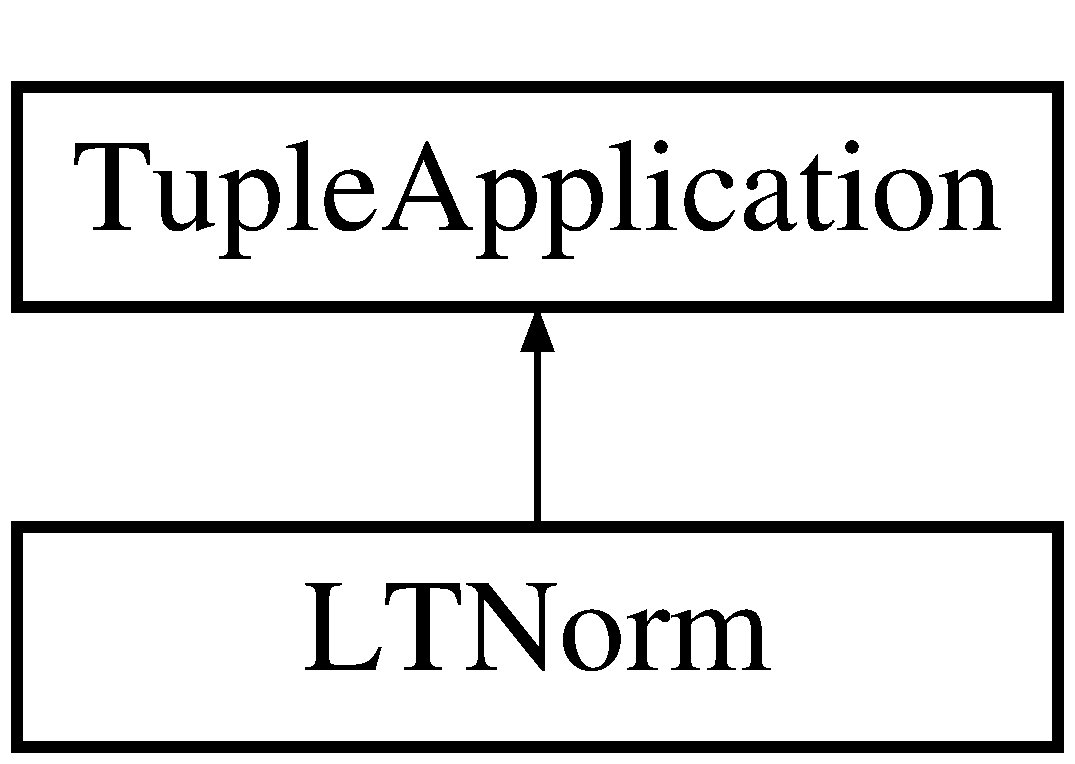
\includegraphics[height=2cm]{class_l_t_norm}
\end{center}
\end{figure}
\subsection*{Protected Member Functions}
\begin{CompactItemize}
\item 
void \hyperlink{class_l_t_norm_58c0b2b050ac4e0fd5927fff451ae9ff}{consumeInput} ()
\item 
void \hyperlink{class_l_t_norm_f0905a2c85b2e2713e98b9b22714a022}{work} ()
\item 
void \hyperlink{class_l_t_norm_2e142e5c7fabd218436f2abe99f4535b}{produceOutput} ()
\end{CompactItemize}
\subsection*{Static Protected Attributes}
\begin{CompactItemize}
\item 
static const char $\ast$ \hyperlink{class_l_t_norm_2df7b3b8cefbb49106f51ba258b1bdd4}{MIN\_\-POINT} = \char`\"{}norm minPoint\char`\"{}
\item 
static const char $\ast$ \hyperlink{class_l_t_norm_54deb1fe0a9ad3f7244a25963aafdec7}{MAX\_\-POINT} = \char`\"{}norm maxPoint\char`\"{}
\end{CompactItemize}


\subsection{Detailed Description}
Re-scales the points in the cloud so that they all lay in the unit square. 

\subsection{Member Function Documentation}
\hypertarget{class_l_t_norm_58c0b2b050ac4e0fd5927fff451ae9ff}{
\index{LTNorm@{LTNorm}!consumeInput@{consumeInput}}
\index{consumeInput@{consumeInput}!LTNorm@{LTNorm}}
\subsubsection[{consumeInput}]{\setlength{\rightskip}{0pt plus 5cm}void LTNorm::consumeInput ()\hspace{0.3cm}{\tt  \mbox{[}protected, virtual\mbox{]}}}}
\label{class_l_t_norm_58c0b2b050ac4e0fd5927fff451ae9ff}


The consume input process is spawned once and should distribute tasks to the worker processes. 

Implements \hyperlink{class_tuple_application_e163c5a536de01c8b94b49528a17dab2}{TupleApplication}.\hypertarget{class_l_t_norm_2e142e5c7fabd218436f2abe99f4535b}{
\index{LTNorm@{LTNorm}!produceOutput@{produceOutput}}
\index{produceOutput@{produceOutput}!LTNorm@{LTNorm}}
\subsubsection[{produceOutput}]{\setlength{\rightskip}{0pt plus 5cm}void LTNorm::produceOutput ()\hspace{0.3cm}{\tt  \mbox{[}protected, virtual\mbox{]}}}}
\label{class_l_t_norm_2e142e5c7fabd218436f2abe99f4535b}


The output producer decides when the tuple application is finished; once this function returns, the tuple application is complete. 

Implements \hyperlink{class_tuple_application_8743dfcf17dedd52887c0b2ab170d8dc}{TupleApplication}.\hypertarget{class_l_t_norm_f0905a2c85b2e2713e98b9b22714a022}{
\index{LTNorm@{LTNorm}!work@{work}}
\index{work@{work}!LTNorm@{LTNorm}}
\subsubsection[{work}]{\setlength{\rightskip}{0pt plus 5cm}void LTNorm::work ()\hspace{0.3cm}{\tt  \mbox{[}protected, virtual\mbox{]}}}}
\label{class_l_t_norm_f0905a2c85b2e2713e98b9b22714a022}


Worker processes are created and killed after the output process has finished. 

Implements \hyperlink{class_tuple_application_ef6ae8bb1d697e4ed038b43320183c89}{TupleApplication}.

\subsection{Member Data Documentation}
\hypertarget{class_l_t_norm_54deb1fe0a9ad3f7244a25963aafdec7}{
\index{LTNorm@{LTNorm}!MAX\_\-POINT@{MAX\_\-POINT}}
\index{MAX\_\-POINT@{MAX\_\-POINT}!LTNorm@{LTNorm}}
\subsubsection[{MAX\_\-POINT}]{\setlength{\rightskip}{0pt plus 5cm}const char $\ast$ {\bf LTNorm::MAX\_\-POINT} = \char`\"{}norm maxPoint\char`\"{}\hspace{0.3cm}{\tt  \mbox{[}static, protected\mbox{]}}}}
\label{class_l_t_norm_54deb1fe0a9ad3f7244a25963aafdec7}


The largest point (in x and y) found \hypertarget{class_l_t_norm_2df7b3b8cefbb49106f51ba258b1bdd4}{
\index{LTNorm@{LTNorm}!MIN\_\-POINT@{MIN\_\-POINT}}
\index{MIN\_\-POINT@{MIN\_\-POINT}!LTNorm@{LTNorm}}
\subsubsection[{MIN\_\-POINT}]{\setlength{\rightskip}{0pt plus 5cm}const char $\ast$ {\bf LTNorm::MIN\_\-POINT} = \char`\"{}norm minPoint\char`\"{}\hspace{0.3cm}{\tt  \mbox{[}static, protected\mbox{]}}}}
\label{class_l_t_norm_2df7b3b8cefbb49106f51ba258b1bdd4}


The smallest point (in x and y) found 

The documentation for this class was generated from the following files:\begin{CompactItemize}
\item 
cowichan\_\-lt/src/\hyperlink{norm_8hpp}{norm.hpp}\item 
cowichan\_\-lt/src/\hyperlink{cowichan__lt_2src_2norm_8cpp}{norm.cpp}\end{CompactItemize}

\hypertarget{class_l_t_outer}{
\section{LTOuter Class Reference}
\label{class_l_t_outer}\index{LTOuter@{LTOuter}}
}
{\tt \#include $<$outer.hpp$>$}

Inheritance diagram for LTOuter::\begin{figure}[H]
\begin{center}
\leavevmode
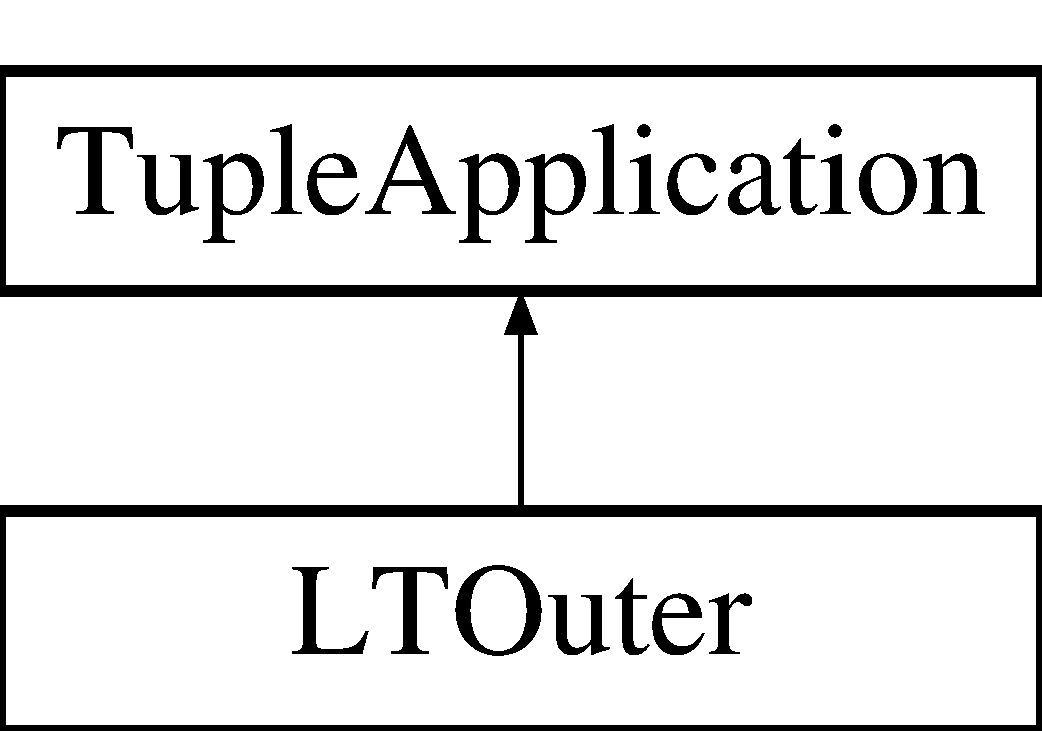
\includegraphics[height=2cm]{class_l_t_outer}
\end{center}
\end{figure}
\subsection*{Protected Member Functions}
\begin{CompactItemize}
\item 
void \hyperlink{class_l_t_outer_3e0493a0d06fbc86fe614edbd752eb8a}{consumeInput} ()
\item 
void \hyperlink{class_l_t_outer_e0b1322b40271bb94c272b6117c8d16c}{work} ()
\item 
void \hyperlink{class_l_t_outer_2a12a006761b2e1132b84209d29fddac}{produceOutput} ()
\end{CompactItemize}
\subsection*{Static Protected Attributes}
\begin{CompactItemize}
\item 
static const char $\ast$ \hyperlink{class_l_t_outer_39056ff036f5138e2f7529c804698bb4}{SYNCH\_\-LOCK} = \char`\"{}outer synch lock\char`\"{}
\item 
static const char $\ast$ \hyperlink{class_l_t_outer_6941f4f6ba366cff85accf2adc955a66}{REQUEST} = \char`\"{}outer request\char`\"{}
\item 
static const char $\ast$ \hyperlink{class_l_t_outer_3a27e2c7371866691ebe47def5db76fa}{MAX\_\-DISTANCE} = \char`\"{}outer max distance\char`\"{}
\item 
static const char $\ast$ \hyperlink{class_l_t_outer_b1e7e3c0471f26305f697f1324f769fa}{MATRIX\_\-ENTRY} = \char`\"{}outer matrix entry\char`\"{}
\end{CompactItemize}


\subsection{Detailed Description}
Performs the outer product with LinuxTuples. 

\subsection{Member Function Documentation}
\hypertarget{class_l_t_outer_3e0493a0d06fbc86fe614edbd752eb8a}{
\index{LTOuter@{LTOuter}!consumeInput@{consumeInput}}
\index{consumeInput@{consumeInput}!LTOuter@{LTOuter}}
\subsubsection[{consumeInput}]{\setlength{\rightskip}{0pt plus 5cm}void LTOuter::consumeInput ()\hspace{0.3cm}{\tt  \mbox{[}protected, virtual\mbox{]}}}}
\label{class_l_t_outer_3e0493a0d06fbc86fe614edbd752eb8a}


The consume input process is spawned once and should distribute tasks to the worker processes. 

Implements \hyperlink{class_tuple_application_e163c5a536de01c8b94b49528a17dab2}{TupleApplication}.\hypertarget{class_l_t_outer_2a12a006761b2e1132b84209d29fddac}{
\index{LTOuter@{LTOuter}!produceOutput@{produceOutput}}
\index{produceOutput@{produceOutput}!LTOuter@{LTOuter}}
\subsubsection[{produceOutput}]{\setlength{\rightskip}{0pt plus 5cm}void LTOuter::produceOutput ()\hspace{0.3cm}{\tt  \mbox{[}protected, virtual\mbox{]}}}}
\label{class_l_t_outer_2a12a006761b2e1132b84209d29fddac}


The output producer decides when the tuple application is finished; once this function returns, the tuple application is complete. 

Implements \hyperlink{class_tuple_application_8743dfcf17dedd52887c0b2ab170d8dc}{TupleApplication}.\hypertarget{class_l_t_outer_e0b1322b40271bb94c272b6117c8d16c}{
\index{LTOuter@{LTOuter}!work@{work}}
\index{work@{work}!LTOuter@{LTOuter}}
\subsubsection[{work}]{\setlength{\rightskip}{0pt plus 5cm}void LTOuter::work ()\hspace{0.3cm}{\tt  \mbox{[}protected, virtual\mbox{]}}}}
\label{class_l_t_outer_e0b1322b40271bb94c272b6117c8d16c}


Worker processes are created and killed after the output process has finished. 

Implements \hyperlink{class_tuple_application_ef6ae8bb1d697e4ed038b43320183c89}{TupleApplication}.

\subsection{Member Data Documentation}
\hypertarget{class_l_t_outer_b1e7e3c0471f26305f697f1324f769fa}{
\index{LTOuter@{LTOuter}!MATRIX\_\-ENTRY@{MATRIX\_\-ENTRY}}
\index{MATRIX\_\-ENTRY@{MATRIX\_\-ENTRY}!LTOuter@{LTOuter}}
\subsubsection[{MATRIX\_\-ENTRY}]{\setlength{\rightskip}{0pt plus 5cm}const char $\ast$ {\bf LTOuter::MATRIX\_\-ENTRY} = \char`\"{}outer matrix entry\char`\"{}\hspace{0.3cm}{\tt  \mbox{[}static, protected\mbox{]}}}}
\label{class_l_t_outer_b1e7e3c0471f26305f697f1324f769fa}


An entry in the matrix, to be stored in the output. \hypertarget{class_l_t_outer_3a27e2c7371866691ebe47def5db76fa}{
\index{LTOuter@{LTOuter}!MAX\_\-DISTANCE@{MAX\_\-DISTANCE}}
\index{MAX\_\-DISTANCE@{MAX\_\-DISTANCE}!LTOuter@{LTOuter}}
\subsubsection[{MAX\_\-DISTANCE}]{\setlength{\rightskip}{0pt plus 5cm}const char $\ast$ {\bf LTOuter::MAX\_\-DISTANCE} = \char`\"{}outer max distance\char`\"{}\hspace{0.3cm}{\tt  \mbox{[}static, protected\mbox{]}}}}
\label{class_l_t_outer_3a27e2c7371866691ebe47def5db76fa}


The maximum length of any vector. \hypertarget{class_l_t_outer_6941f4f6ba366cff85accf2adc955a66}{
\index{LTOuter@{LTOuter}!REQUEST@{REQUEST}}
\index{REQUEST@{REQUEST}!LTOuter@{LTOuter}}
\subsubsection[{REQUEST}]{\setlength{\rightskip}{0pt plus 5cm}const char $\ast$ {\bf LTOuter::REQUEST} = \char`\"{}outer request\char`\"{}\hspace{0.3cm}{\tt  \mbox{[}static, protected\mbox{]}}}}
\label{class_l_t_outer_6941f4f6ba366cff85accf2adc955a66}


Request to compute for one vector. \hypertarget{class_l_t_outer_39056ff036f5138e2f7529c804698bb4}{
\index{LTOuter@{LTOuter}!SYNCH\_\-LOCK@{SYNCH\_\-LOCK}}
\index{SYNCH\_\-LOCK@{SYNCH\_\-LOCK}!LTOuter@{LTOuter}}
\subsubsection[{SYNCH\_\-LOCK}]{\setlength{\rightskip}{0pt plus 5cm}const char $\ast$ {\bf LTOuter::SYNCH\_\-LOCK} = \char`\"{}outer synch lock\char`\"{}\hspace{0.3cm}{\tt  \mbox{[}static, protected\mbox{]}}}}
\label{class_l_t_outer_39056ff036f5138e2f7529c804698bb4}


Synchronization lock (critical section). 

The documentation for this class was generated from the following files:\begin{CompactItemize}
\item 
cowichan\_\-lt/src/\hyperlink{outer_8hpp}{outer.hpp}\item 
cowichan\_\-lt/src/\hyperlink{cowichan__lt_2src_2outer_8cpp}{outer.cpp}\end{CompactItemize}

\hypertarget{class_l_t_product}{
\section{LTProduct Class Reference}
\label{class_l_t_product}\index{LTProduct@{LTProduct}}
}
{\tt \#include $<$product.hpp$>$}

Inheritance diagram for LTProduct::\begin{figure}[H]
\begin{center}
\leavevmode
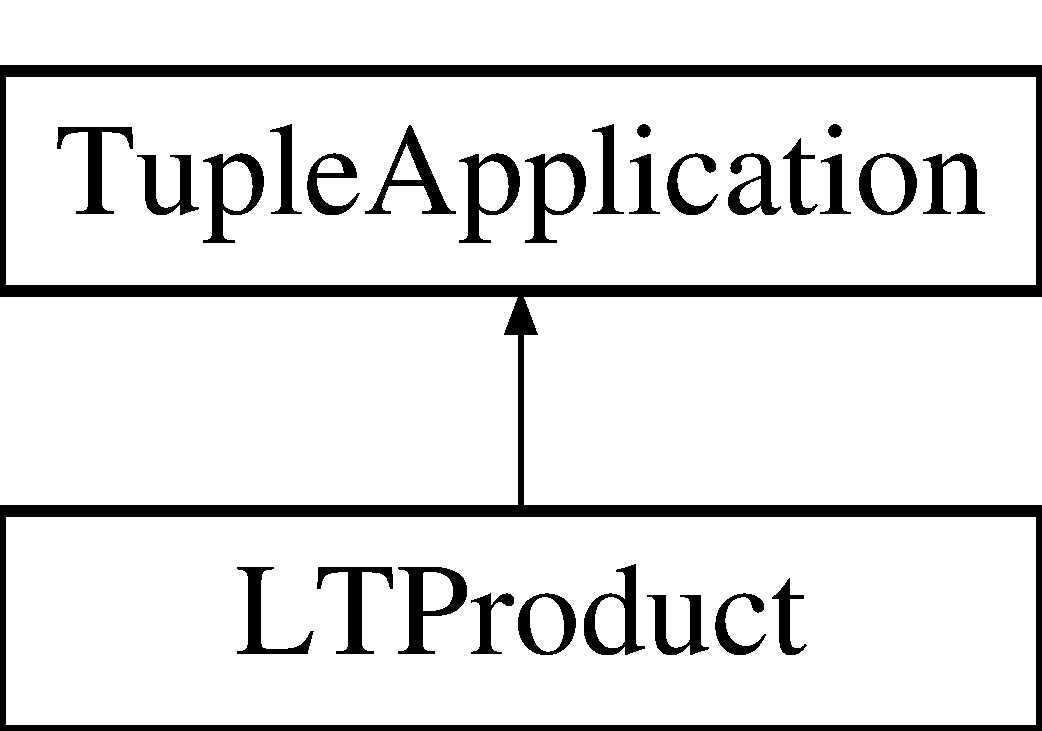
\includegraphics[height=2cm]{class_l_t_product}
\end{center}
\end{figure}
\subsection*{Protected Member Functions}
\begin{CompactItemize}
\item 
void \hyperlink{class_l_t_product_377454ff007fa15f0bd378013bf1e6e6}{consumeInput} ()
\item 
void \hyperlink{class_l_t_product_1ba17b14e59b82c917f404cc9642bb09}{work} ()
\item 
void \hyperlink{class_l_t_product_d03b068863d7b2febcbb7b11ebb819ca}{produceOutput} ()
\end{CompactItemize}


\subsection{Detailed Description}
Performs the product of a matrix and a vector in tuple-space. 

\subsection{Member Function Documentation}
\hypertarget{class_l_t_product_377454ff007fa15f0bd378013bf1e6e6}{
\index{LTProduct@{LTProduct}!consumeInput@{consumeInput}}
\index{consumeInput@{consumeInput}!LTProduct@{LTProduct}}
\subsubsection[{consumeInput}]{\setlength{\rightskip}{0pt plus 5cm}void LTProduct::consumeInput ()\hspace{0.3cm}{\tt  \mbox{[}protected, virtual\mbox{]}}}}
\label{class_l_t_product_377454ff007fa15f0bd378013bf1e6e6}


The consume input process is spawned once and should distribute tasks to the worker processes. 

Implements \hyperlink{class_tuple_application_e163c5a536de01c8b94b49528a17dab2}{TupleApplication}.\hypertarget{class_l_t_product_d03b068863d7b2febcbb7b11ebb819ca}{
\index{LTProduct@{LTProduct}!produceOutput@{produceOutput}}
\index{produceOutput@{produceOutput}!LTProduct@{LTProduct}}
\subsubsection[{produceOutput}]{\setlength{\rightskip}{0pt plus 5cm}void LTProduct::produceOutput ()\hspace{0.3cm}{\tt  \mbox{[}protected, virtual\mbox{]}}}}
\label{class_l_t_product_d03b068863d7b2febcbb7b11ebb819ca}


The output producer decides when the tuple application is finished; once this function returns, the tuple application is complete. 

Implements \hyperlink{class_tuple_application_8743dfcf17dedd52887c0b2ab170d8dc}{TupleApplication}.\hypertarget{class_l_t_product_1ba17b14e59b82c917f404cc9642bb09}{
\index{LTProduct@{LTProduct}!work@{work}}
\index{work@{work}!LTProduct@{LTProduct}}
\subsubsection[{work}]{\setlength{\rightskip}{0pt plus 5cm}void LTProduct::work ()\hspace{0.3cm}{\tt  \mbox{[}protected, virtual\mbox{]}}}}
\label{class_l_t_product_1ba17b14e59b82c917f404cc9642bb09}


Worker processes are created and killed after the output process has finished. 

Implements \hyperlink{class_tuple_application_ef6ae8bb1d697e4ed038b43320183c89}{TupleApplication}.

The documentation for this class was generated from the following files:\begin{CompactItemize}
\item 
cowichan\_\-lt/src/\hyperlink{product_8hpp}{product.hpp}\item 
cowichan\_\-lt/src/\hyperlink{cowichan__lt_2src_2product_8cpp}{product.cpp}\end{CompactItemize}

\hypertarget{class_l_t_randmat}{
\section{LTRandmat Class Reference}
\label{class_l_t_randmat}\index{LTRandmat@{LTRandmat}}
}
{\tt \#include $<$randmat.hpp$>$}

Inheritance diagram for LTRandmat::\begin{figure}[H]
\begin{center}
\leavevmode
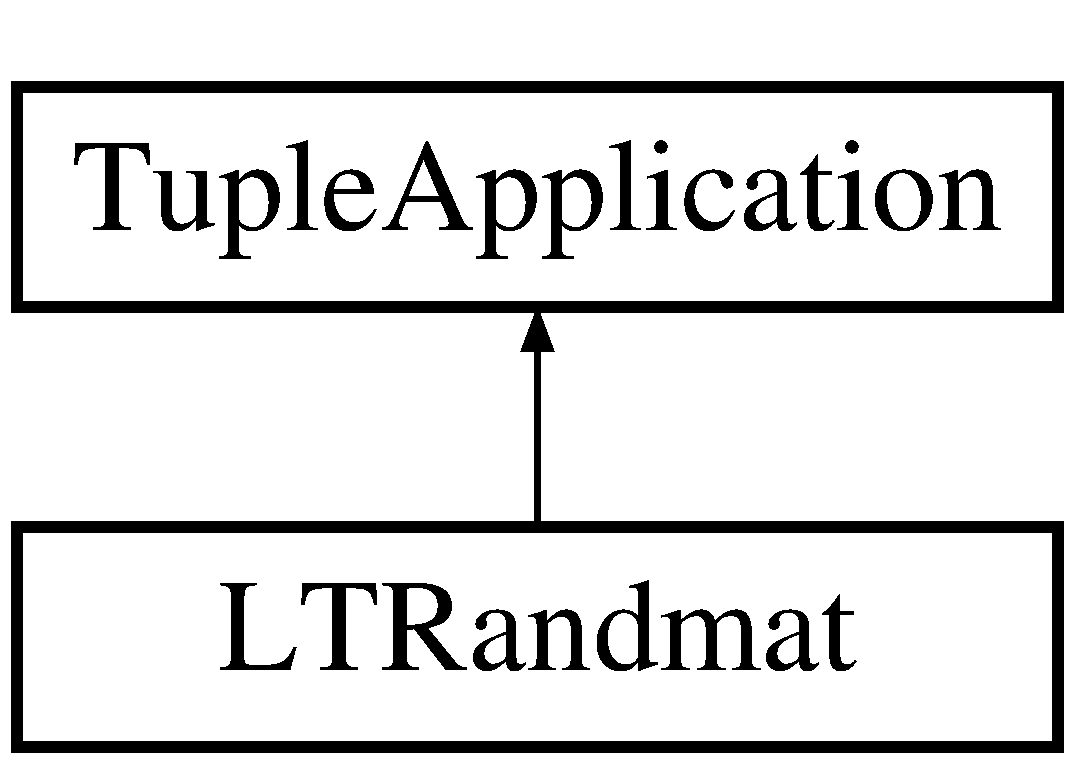
\includegraphics[height=2cm]{class_l_t_randmat}
\end{center}
\end{figure}
\subsection*{Protected Member Functions}
\begin{CompactItemize}
\item 
void \hyperlink{class_l_t_randmat_73181e409565b18c77d880dbf4123b26}{consumeInput} ()
\item 
void \hyperlink{class_l_t_randmat_fffb75c16f2aaaa2f1bdb8a52f79234c}{work} ()
\item 
void \hyperlink{class_l_t_randmat_3adc0a50f5840dcc1228f4449e2b5da3}{produceOutput} ()
\item 
void \hyperlink{class_l_t_randmat_7c807565838d1882d33d183e90575653}{setup} ()
\item 
\hyperlink{cowichan_8hpp_c96945095fd0ce7186a1d00a89f77d2c}{INT\_\-TYPE} \hyperlink{class_l_t_randmat_cf34e6e21b7b22b315f9c8df37646448}{next} (\hyperlink{cowichan_8hpp_c96945095fd0ce7186a1d00a89f77d2c}{INT\_\-TYPE} \&current) const 
\end{CompactItemize}
\subsection*{Protected Attributes}
\begin{CompactItemize}
\item 
\hyperlink{cowichan_8hpp_c96945095fd0ce7186a1d00a89f77d2c}{INT\_\-TYPE} \hyperlink{class_l_t_randmat_eaa83f04ca349926529a5f69249358f2}{aPrime}
\item 
\hyperlink{cowichan_8hpp_c96945095fd0ce7186a1d00a89f77d2c}{INT\_\-TYPE} \hyperlink{class_l_t_randmat_419c5347dd2f402355088d51e03e8325}{cPrime}
\end{CompactItemize}
\subsection*{Static Protected Attributes}
\begin{CompactItemize}
\item 
static const char $\ast$ \hyperlink{class_l_t_randmat_0eb3b36daa68b21b70215c437976c849}{REQUEST} = \char`\"{}randmat request\char`\"{}
\end{CompactItemize}


\subsection{Detailed Description}
Tuple application to solve the bulk of the randmat cowichan problem. 

\subsection{Member Function Documentation}
\hypertarget{class_l_t_randmat_73181e409565b18c77d880dbf4123b26}{
\index{LTRandmat@{LTRandmat}!consumeInput@{consumeInput}}
\index{consumeInput@{consumeInput}!LTRandmat@{LTRandmat}}
\subsubsection[{consumeInput}]{\setlength{\rightskip}{0pt plus 5cm}void LTRandmat::consumeInput ()\hspace{0.3cm}{\tt  \mbox{[}protected, virtual\mbox{]}}}}
\label{class_l_t_randmat_73181e409565b18c77d880dbf4123b26}


The consume input process is spawned once and should distribute tasks to the worker processes. 

Implements \hyperlink{class_tuple_application_e163c5a536de01c8b94b49528a17dab2}{TupleApplication}.\hypertarget{class_l_t_randmat_cf34e6e21b7b22b315f9c8df37646448}{
\index{LTRandmat@{LTRandmat}!next@{next}}
\index{next@{next}!LTRandmat@{LTRandmat}}
\subsubsection[{next}]{\setlength{\rightskip}{0pt plus 5cm}{\bf INT\_\-TYPE} LTRandmat::next ({\bf INT\_\-TYPE} \& {\em current}) const\hspace{0.3cm}{\tt  \mbox{[}inline, protected\mbox{]}}}}
\label{class_l_t_randmat_cf34e6e21b7b22b315f9c8df37646448}


Computes the next value in the random sequence. \begin{Desc}
\item[Parameters:]
\begin{description}
\item[{\em current}]the previous value in the random sequence. \end{description}
\end{Desc}
\begin{Desc}
\item[Returns:]the next value in the random sequence. \end{Desc}
\hypertarget{class_l_t_randmat_3adc0a50f5840dcc1228f4449e2b5da3}{
\index{LTRandmat@{LTRandmat}!produceOutput@{produceOutput}}
\index{produceOutput@{produceOutput}!LTRandmat@{LTRandmat}}
\subsubsection[{produceOutput}]{\setlength{\rightskip}{0pt plus 5cm}void LTRandmat::produceOutput ()\hspace{0.3cm}{\tt  \mbox{[}protected, virtual\mbox{]}}}}
\label{class_l_t_randmat_3adc0a50f5840dcc1228f4449e2b5da3}


The output producer decides when the tuple application is finished; once this function returns, the tuple application is complete. 

Implements \hyperlink{class_tuple_application_8743dfcf17dedd52887c0b2ab170d8dc}{TupleApplication}.\hypertarget{class_l_t_randmat_7c807565838d1882d33d183e90575653}{
\index{LTRandmat@{LTRandmat}!setup@{setup}}
\index{setup@{setup}!LTRandmat@{LTRandmat}}
\subsubsection[{setup}]{\setlength{\rightskip}{0pt plus 5cm}void LTRandmat::setup ()\hspace{0.3cm}{\tt  \mbox{[}protected\mbox{]}}}}
\label{class_l_t_randmat_7c807565838d1882d33d183e90575653}


Create the first, seed column. \hypertarget{class_l_t_randmat_fffb75c16f2aaaa2f1bdb8a52f79234c}{
\index{LTRandmat@{LTRandmat}!work@{work}}
\index{work@{work}!LTRandmat@{LTRandmat}}
\subsubsection[{work}]{\setlength{\rightskip}{0pt plus 5cm}void LTRandmat::work ()\hspace{0.3cm}{\tt  \mbox{[}protected, virtual\mbox{]}}}}
\label{class_l_t_randmat_fffb75c16f2aaaa2f1bdb8a52f79234c}


Worker processes are created and killed after the output process has finished. 

Implements \hyperlink{class_tuple_application_ef6ae8bb1d697e4ed038b43320183c89}{TupleApplication}.

\subsection{Member Data Documentation}
\hypertarget{class_l_t_randmat_eaa83f04ca349926529a5f69249358f2}{
\index{LTRandmat@{LTRandmat}!aPrime@{aPrime}}
\index{aPrime@{aPrime}!LTRandmat@{LTRandmat}}
\subsubsection[{aPrime}]{\setlength{\rightskip}{0pt plus 5cm}{\bf INT\_\-TYPE} {\bf LTRandmat::aPrime}\hspace{0.3cm}{\tt  \mbox{[}protected\mbox{]}}}}
\label{class_l_t_randmat_eaa83f04ca349926529a5f69249358f2}


A value to use for the next-K parallel randmat computation. \hypertarget{class_l_t_randmat_419c5347dd2f402355088d51e03e8325}{
\index{LTRandmat@{LTRandmat}!cPrime@{cPrime}}
\index{cPrime@{cPrime}!LTRandmat@{LTRandmat}}
\subsubsection[{cPrime}]{\setlength{\rightskip}{0pt plus 5cm}{\bf INT\_\-TYPE} {\bf LTRandmat::cPrime}\hspace{0.3cm}{\tt  \mbox{[}protected\mbox{]}}}}
\label{class_l_t_randmat_419c5347dd2f402355088d51e03e8325}


C value to use for the next-K parallel randmat computation. \hypertarget{class_l_t_randmat_0eb3b36daa68b21b70215c437976c849}{
\index{LTRandmat@{LTRandmat}!REQUEST@{REQUEST}}
\index{REQUEST@{REQUEST}!LTRandmat@{LTRandmat}}
\subsubsection[{REQUEST}]{\setlength{\rightskip}{0pt plus 5cm}const char $\ast$ {\bf LTRandmat::REQUEST} = \char`\"{}randmat request\char`\"{}\hspace{0.3cm}{\tt  \mbox{[}static, protected\mbox{]}}}}
\label{class_l_t_randmat_0eb3b36daa68b21b70215c437976c849}


Request for a grid row to be generated. 

The documentation for this class was generated from the following files:\begin{CompactItemize}
\item 
cowichan\_\-lt/src/\hyperlink{randmat_8hpp}{randmat.hpp}\item 
cowichan\_\-lt/src/\hyperlink{cowichan__lt_2src_2randmat_8cpp}{randmat.cpp}\end{CompactItemize}

\hypertarget{class_l_t_sor}{
\section{LTSor Class Reference}
\label{class_l_t_sor}\index{LTSor@{LTSor}}
}
{\tt \#include $<$sor.hpp$>$}

Inheritance diagram for LTSor::\begin{figure}[H]
\begin{center}
\leavevmode
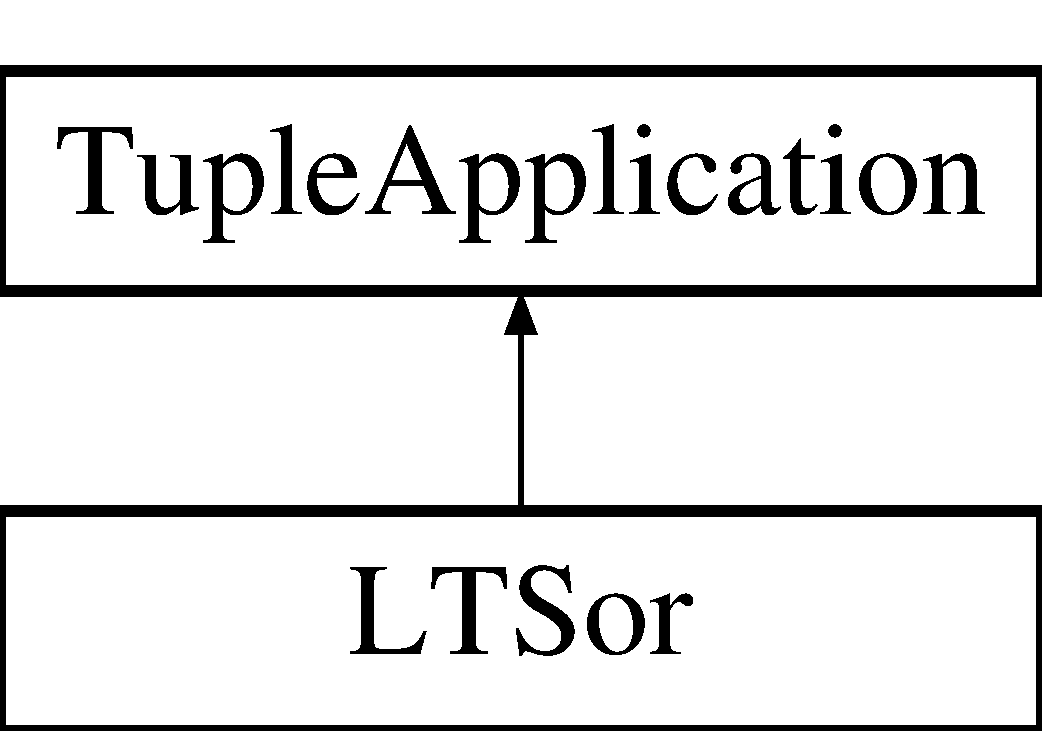
\includegraphics[height=2cm]{class_l_t_sor}
\end{center}
\end{figure}
\subsection*{Protected Member Functions}
\begin{CompactItemize}
\item 
void \hyperlink{class_l_t_sor_4fc4f0f914fc08f57f2ef5ba346cef1d}{consumeInput} ()
\item 
void \hyperlink{class_l_t_sor_48363c30cbba1c5ca61ed86260db94af}{work} ()
\item 
void \hyperlink{class_l_t_sor_19e969a6ab342ee86d86721fbd37e7a6}{produceOutput} ()
\item 
\hyperlink{cowichan_8hpp_4d521b2c54a1f6312cc8fa04827eaf98}{real} \hyperlink{class_l_t_sor_c4a890faff8c1caeb6089b0b8b488e38}{solutionSum} (\hyperlink{cowichan_8hpp_5b04577d5d21124855deaad298595371}{index\_\-t} row)
\end{CompactItemize}
\subsection*{Static Protected Attributes}
\begin{CompactItemize}
\item 
static const char $\ast$ \hyperlink{class_l_t_sor_bc947063bba409b5b9a1a06e1ddb2070}{SYNCH\_\-LOCK} = \char`\"{}sor synch lock\char`\"{}
\item 
static const char $\ast$ \hyperlink{class_l_t_sor_0276e790a83efc366011482c3e8597c4}{ROWS\_\-DONE} = \char`\"{}sor rows reporting\char`\"{}
\item 
static const char $\ast$ \hyperlink{class_l_t_sor_913b683357eabbd90a363da6459c8794}{SOLUTION\_\-VECTOR} = \char`\"{}sor solution row\char`\"{}
\item 
static const char $\ast$ \hyperlink{class_l_t_sor_b70b582671901d2b4680e82fd756cf1f}{SOLUTION\_\-SUM} = \char`\"{}sor inner sum\char`\"{}
\item 
static const char $\ast$ \hyperlink{class_l_t_sor_2784b20dce735b35e3ac40b26b1df40a}{SOR\_\-FLAG} = \char`\"{}sor input consumed\char`\"{}
\end{CompactItemize}


\subsection{Detailed Description}
Performs a successive over-relaxation to solve a matrix problem Ax = b. The solution is approximate, but it can be made arbitrarily accurate. The computation is done in tuple space. 

\subsection{Member Function Documentation}
\hypertarget{class_l_t_sor_4fc4f0f914fc08f57f2ef5ba346cef1d}{
\index{LTSor@{LTSor}!consumeInput@{consumeInput}}
\index{consumeInput@{consumeInput}!LTSor@{LTSor}}
\subsubsection[{consumeInput}]{\setlength{\rightskip}{0pt plus 5cm}void LTSor::consumeInput ()\hspace{0.3cm}{\tt  \mbox{[}protected, virtual\mbox{]}}}}
\label{class_l_t_sor_4fc4f0f914fc08f57f2ef5ba346cef1d}


The consume input process is spawned once and should distribute tasks to the worker processes. 

Implements \hyperlink{class_tuple_application_e163c5a536de01c8b94b49528a17dab2}{TupleApplication}.\hypertarget{class_l_t_sor_19e969a6ab342ee86d86721fbd37e7a6}{
\index{LTSor@{LTSor}!produceOutput@{produceOutput}}
\index{produceOutput@{produceOutput}!LTSor@{LTSor}}
\subsubsection[{produceOutput}]{\setlength{\rightskip}{0pt plus 5cm}void LTSor::produceOutput ()\hspace{0.3cm}{\tt  \mbox{[}protected, virtual\mbox{]}}}}
\label{class_l_t_sor_19e969a6ab342ee86d86721fbd37e7a6}


The output producer decides when the tuple application is finished; once this function returns, the tuple application is complete. 

Implements \hyperlink{class_tuple_application_8743dfcf17dedd52887c0b2ab170d8dc}{TupleApplication}.\hypertarget{class_l_t_sor_c4a890faff8c1caeb6089b0b8b488e38}{
\index{LTSor@{LTSor}!solutionSum@{solutionSum}}
\index{solutionSum@{solutionSum}!LTSor@{LTSor}}
\subsubsection[{solutionSum}]{\setlength{\rightskip}{0pt plus 5cm}{\bf real} LTSor::solutionSum ({\bf index\_\-t} {\em row})\hspace{0.3cm}{\tt  \mbox{[}protected\mbox{]}}}}
\label{class_l_t_sor_c4a890faff8c1caeb6089b0b8b488e38}


Performs the sum portion of the SOR processor. \begin{Desc}
\item[Parameters:]
\begin{description}
\item[{\em row}]the row to perform on. \end{description}
\end{Desc}
\begin{Desc}
\item[Returns:]the sum. \end{Desc}
\hypertarget{class_l_t_sor_48363c30cbba1c5ca61ed86260db94af}{
\index{LTSor@{LTSor}!work@{work}}
\index{work@{work}!LTSor@{LTSor}}
\subsubsection[{work}]{\setlength{\rightskip}{0pt plus 5cm}void LTSor::work ()\hspace{0.3cm}{\tt  \mbox{[}protected, virtual\mbox{]}}}}
\label{class_l_t_sor_48363c30cbba1c5ca61ed86260db94af}


Worker processes are created and killed after the output process has finished. 

Implements \hyperlink{class_tuple_application_ef6ae8bb1d697e4ed038b43320183c89}{TupleApplication}.

\subsection{Member Data Documentation}
\hypertarget{class_l_t_sor_0276e790a83efc366011482c3e8597c4}{
\index{LTSor@{LTSor}!ROWS\_\-DONE@{ROWS\_\-DONE}}
\index{ROWS\_\-DONE@{ROWS\_\-DONE}!LTSor@{LTSor}}
\subsubsection[{ROWS\_\-DONE}]{\setlength{\rightskip}{0pt plus 5cm}const char $\ast$ {\bf LTSor::ROWS\_\-DONE} = \char`\"{}sor rows reporting\char`\"{}\hspace{0.3cm}{\tt  \mbox{[}static, protected\mbox{]}}}}
\label{class_l_t_sor_0276e790a83efc366011482c3e8597c4}


The number of rows done in the middle SOR section. \hypertarget{class_l_t_sor_b70b582671901d2b4680e82fd756cf1f}{
\index{LTSor@{LTSor}!SOLUTION\_\-SUM@{SOLUTION\_\-SUM}}
\index{SOLUTION\_\-SUM@{SOLUTION\_\-SUM}!LTSor@{LTSor}}
\subsubsection[{SOLUTION\_\-SUM}]{\setlength{\rightskip}{0pt plus 5cm}const char $\ast$ {\bf LTSor::SOLUTION\_\-SUM} = \char`\"{}sor inner sum\char`\"{}\hspace{0.3cm}{\tt  \mbox{[}static, protected\mbox{]}}}}
\label{class_l_t_sor_b70b582671901d2b4680e82fd756cf1f}


The on-going sum of the solution. \hypertarget{class_l_t_sor_913b683357eabbd90a363da6459c8794}{
\index{LTSor@{LTSor}!SOLUTION\_\-VECTOR@{SOLUTION\_\-VECTOR}}
\index{SOLUTION\_\-VECTOR@{SOLUTION\_\-VECTOR}!LTSor@{LTSor}}
\subsubsection[{SOLUTION\_\-VECTOR}]{\setlength{\rightskip}{0pt plus 5cm}const char $\ast$ {\bf LTSor::SOLUTION\_\-VECTOR} = \char`\"{}sor solution row\char`\"{}\hspace{0.3cm}{\tt  \mbox{[}static, protected\mbox{]}}}}
\label{class_l_t_sor_913b683357eabbd90a363da6459c8794}


The vector of the solution in tuple space \hypertarget{class_l_t_sor_2784b20dce735b35e3ac40b26b1df40a}{
\index{LTSor@{LTSor}!SOR\_\-FLAG@{SOR\_\-FLAG}}
\index{SOR\_\-FLAG@{SOR\_\-FLAG}!LTSor@{LTSor}}
\subsubsection[{SOR\_\-FLAG}]{\setlength{\rightskip}{0pt plus 5cm}const char $\ast$ {\bf LTSor::SOR\_\-FLAG} = \char`\"{}sor input consumed\char`\"{}\hspace{0.3cm}{\tt  \mbox{[}static, protected\mbox{]}}}}
\label{class_l_t_sor_2784b20dce735b35e3ac40b26b1df40a}


Should we flag the output producer? \hypertarget{class_l_t_sor_bc947063bba409b5b9a1a06e1ddb2070}{
\index{LTSor@{LTSor}!SYNCH\_\-LOCK@{SYNCH\_\-LOCK}}
\index{SYNCH\_\-LOCK@{SYNCH\_\-LOCK}!LTSor@{LTSor}}
\subsubsection[{SYNCH\_\-LOCK}]{\setlength{\rightskip}{0pt plus 5cm}const char $\ast$ {\bf LTSor::SYNCH\_\-LOCK} = \char`\"{}sor synch lock\char`\"{}\hspace{0.3cm}{\tt  \mbox{[}static, protected\mbox{]}}}}
\label{class_l_t_sor_bc947063bba409b5b9a1a06e1ddb2070}


Synchronization lock (critical section). 

The documentation for this class was generated from the following files:\begin{CompactItemize}
\item 
cowichan\_\-lt/src/\hyperlink{sor_8hpp}{sor.hpp}\item 
cowichan\_\-lt/src/\hyperlink{cowichan__lt_2src_2sor_8cpp}{sor.cpp}\end{CompactItemize}

\hypertarget{class_l_t_thresh}{
\section{LTThresh Class Reference}
\label{class_l_t_thresh}\index{LTThresh@{LTThresh}}
}
{\tt \#include $<$thresh.hpp$>$}

Inheritance diagram for LTThresh::\begin{figure}[H]
\begin{center}
\leavevmode
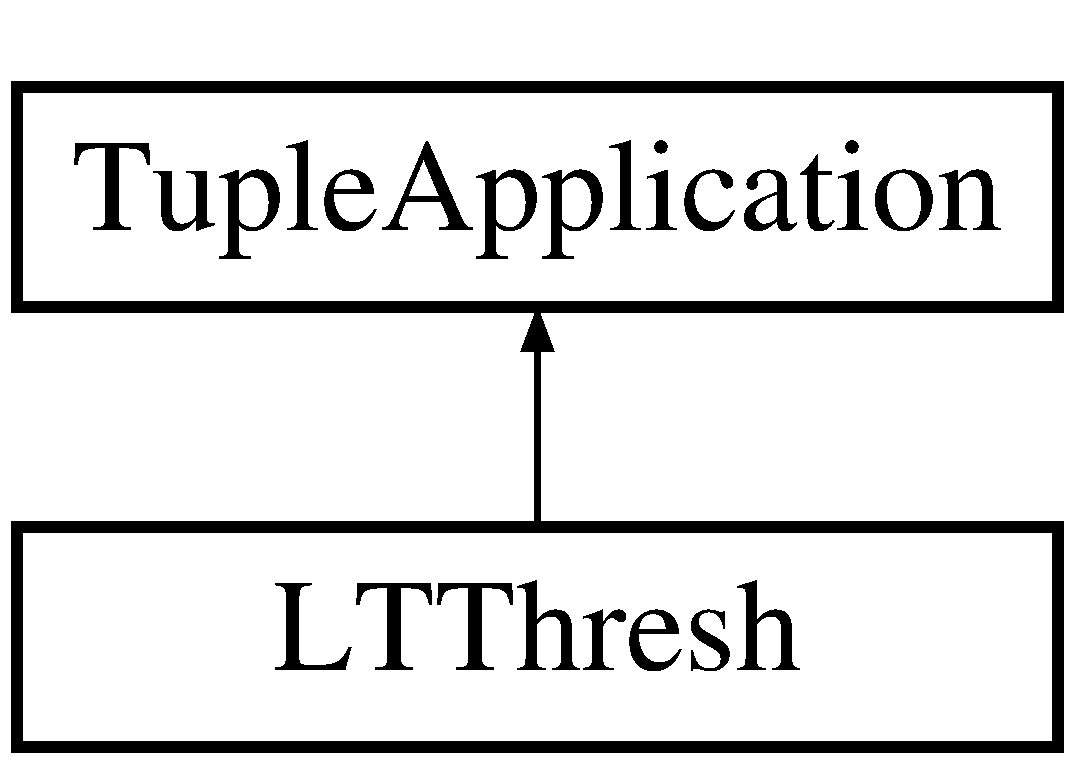
\includegraphics[height=2cm]{class_l_t_thresh}
\end{center}
\end{figure}
\subsection*{Protected Member Functions}
\begin{CompactItemize}
\item 
void \hyperlink{class_l_t_thresh_b802b240b17b2c71cb758e1fe7585d72}{consumeInput} ()
\item 
void \hyperlink{class_l_t_thresh_3cff6d04c7389a32e1dca924c7f93e23}{work} ()
\item 
void \hyperlink{class_l_t_thresh_41ce024f24320a5bd65239e98ac85587}{produceOutput} ()
\end{CompactItemize}
\subsection*{Static Protected Attributes}
\begin{CompactItemize}
\item 
static const char $\ast$ \hyperlink{class_l_t_thresh_2d17b2a1fe255b7d7beaf65d474ef8c0}{REQUEST} = \char`\"{}thresh request\char`\"{}
\item 
static const char $\ast$ \hyperlink{class_l_t_thresh_f249bcd9d3da75f2fb16e2b38451c0c6}{POINT} = \char`\"{}thresh point\char`\"{}
\item 
static const char $\ast$ \hyperlink{class_l_t_thresh_88549a567cbcc63337e0485ad3bad305}{DONE} = \char`\"{}thresh done\char`\"{}
\end{CompactItemize}


\subsection{Detailed Description}
Uses the breaking-point discovered with \hyperlink{class_l_t_frequency}{LTFrequency} to create a boolean matrix of true (above the breaking point) or false (not). 

\subsection{Member Function Documentation}
\hypertarget{class_l_t_thresh_b802b240b17b2c71cb758e1fe7585d72}{
\index{LTThresh@{LTThresh}!consumeInput@{consumeInput}}
\index{consumeInput@{consumeInput}!LTThresh@{LTThresh}}
\subsubsection[{consumeInput}]{\setlength{\rightskip}{0pt plus 5cm}void LTThresh::consumeInput ()\hspace{0.3cm}{\tt  \mbox{[}protected, virtual\mbox{]}}}}
\label{class_l_t_thresh_b802b240b17b2c71cb758e1fe7585d72}


The consume input process is spawned once and should distribute tasks to the worker processes. 

Implements \hyperlink{class_tuple_application_e163c5a536de01c8b94b49528a17dab2}{TupleApplication}.\hypertarget{class_l_t_thresh_41ce024f24320a5bd65239e98ac85587}{
\index{LTThresh@{LTThresh}!produceOutput@{produceOutput}}
\index{produceOutput@{produceOutput}!LTThresh@{LTThresh}}
\subsubsection[{produceOutput}]{\setlength{\rightskip}{0pt plus 5cm}void LTThresh::produceOutput ()\hspace{0.3cm}{\tt  \mbox{[}protected, virtual\mbox{]}}}}
\label{class_l_t_thresh_41ce024f24320a5bd65239e98ac85587}


The output producer decides when the tuple application is finished; once this function returns, the tuple application is complete. 

Implements \hyperlink{class_tuple_application_8743dfcf17dedd52887c0b2ab170d8dc}{TupleApplication}.\hypertarget{class_l_t_thresh_3cff6d04c7389a32e1dca924c7f93e23}{
\index{LTThresh@{LTThresh}!work@{work}}
\index{work@{work}!LTThresh@{LTThresh}}
\subsubsection[{work}]{\setlength{\rightskip}{0pt plus 5cm}void LTThresh::work ()\hspace{0.3cm}{\tt  \mbox{[}protected, virtual\mbox{]}}}}
\label{class_l_t_thresh_3cff6d04c7389a32e1dca924c7f93e23}


Worker processes are created and killed after the output process has finished. 

Implements \hyperlink{class_tuple_application_ef6ae8bb1d697e4ed038b43320183c89}{TupleApplication}.

\subsection{Member Data Documentation}
\hypertarget{class_l_t_thresh_88549a567cbcc63337e0485ad3bad305}{
\index{LTThresh@{LTThresh}!DONE@{DONE}}
\index{DONE@{DONE}!LTThresh@{LTThresh}}
\subsubsection[{DONE}]{\setlength{\rightskip}{0pt plus 5cm}const char $\ast$ {\bf LTThresh::DONE} = \char`\"{}thresh done\char`\"{}\hspace{0.3cm}{\tt  \mbox{[}static, protected\mbox{]}}}}
\label{class_l_t_thresh_88549a567cbcc63337e0485ad3bad305}


Flagged when finished. \hypertarget{class_l_t_thresh_f249bcd9d3da75f2fb16e2b38451c0c6}{
\index{LTThresh@{LTThresh}!POINT@{POINT}}
\index{POINT@{POINT}!LTThresh@{LTThresh}}
\subsubsection[{POINT}]{\setlength{\rightskip}{0pt plus 5cm}const char $\ast$ {\bf LTThresh::POINT} = \char`\"{}thresh point\char`\"{}\hspace{0.3cm}{\tt  \mbox{[}static, protected\mbox{]}}}}
\label{class_l_t_thresh_f249bcd9d3da75f2fb16e2b38451c0c6}


The breaking-point for the thresholding process. \hypertarget{class_l_t_thresh_2d17b2a1fe255b7d7beaf65d474ef8c0}{
\index{LTThresh@{LTThresh}!REQUEST@{REQUEST}}
\index{REQUEST@{REQUEST}!LTThresh@{LTThresh}}
\subsubsection[{REQUEST}]{\setlength{\rightskip}{0pt plus 5cm}const char $\ast$ {\bf LTThresh::REQUEST} = \char`\"{}thresh request\char`\"{}\hspace{0.3cm}{\tt  \mbox{[}static, protected\mbox{]}}}}
\label{class_l_t_thresh_2d17b2a1fe255b7d7beaf65d474ef8c0}


A request to compute a row. 

The documentation for this class was generated from the following files:\begin{CompactItemize}
\item 
cowichan\_\-lt/src/\hyperlink{thresh_8hpp}{thresh.hpp}\item 
cowichan\_\-lt/src/\hyperlink{cowichan__lt_2src_2thresh_8cpp}{thresh.cpp}\end{CompactItemize}

\hypertarget{class_l_t_vecdiff}{
\section{LTVecdiff Class Reference}
\label{class_l_t_vecdiff}\index{LTVecdiff@{LTVecdiff}}
}
{\tt \#include $<$vecdiff.hpp$>$}

Inheritance diagram for LTVecdiff::\begin{figure}[H]
\begin{center}
\leavevmode
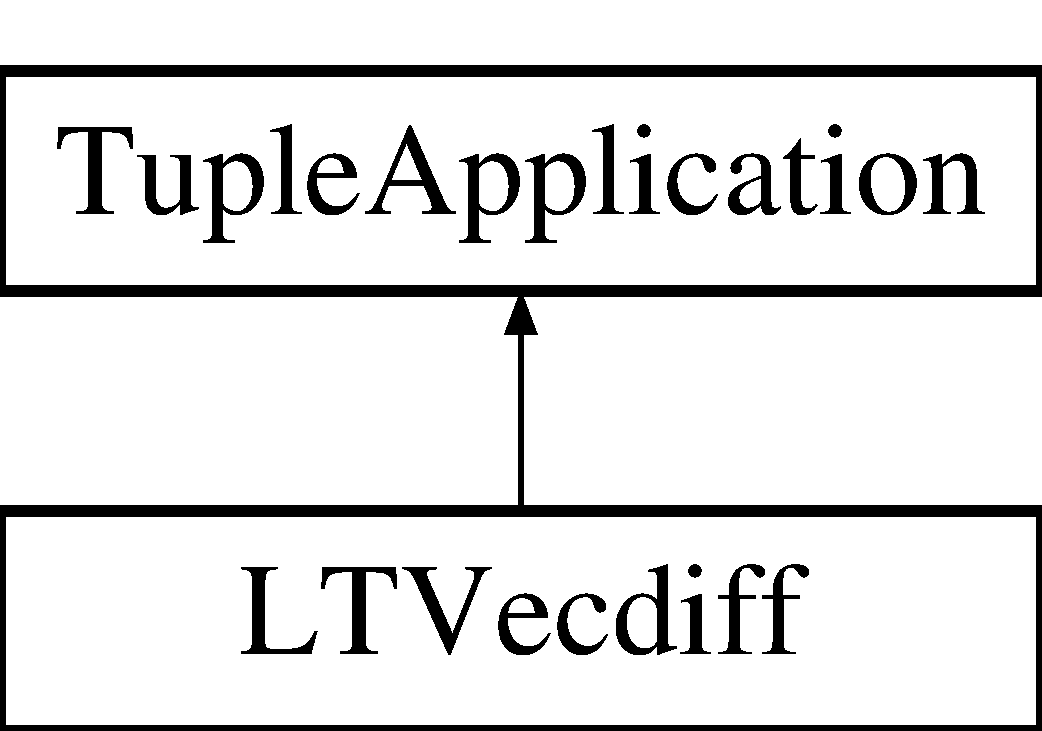
\includegraphics[height=2cm]{class_l_t_vecdiff}
\end{center}
\end{figure}
\subsection*{Protected Member Functions}
\begin{CompactItemize}
\item 
void \hyperlink{class_l_t_vecdiff_9daf31de467c9694e59b55936780dce8}{consumeInput} ()
\item 
void \hyperlink{class_l_t_vecdiff_0117017e12284b1eb57532ca447684f6}{work} ()
\item 
void \hyperlink{class_l_t_vecdiff_69d3c6e3c51052522d474cc75d11a2f2}{produceOutput} ()
\end{CompactItemize}
\subsection*{Static Protected Attributes}
\begin{CompactItemize}
\item 
static const char $\ast$ \hyperlink{class_l_t_vecdiff_251e456901f73b685b41a3826c3a5f8c}{SYNCH\_\-LOCK} = \char`\"{}vecdiff synch lock\char`\"{}
\item 
static const char $\ast$ \hyperlink{class_l_t_vecdiff_552dd71094bbdd099775890405a05221}{ELEMENTS\_\-DONE} = \char`\"{}vecdiff elements reporting\char`\"{}
\item 
static const char $\ast$ \hyperlink{class_l_t_vecdiff_4eecee406e18ced8eef15dfc074d9a55}{MAX\_\-DIFF} = \char`\"{}vecdiff max difference\char`\"{}
\end{CompactItemize}


\subsection{Detailed Description}
Performs the vector difference with LinuxTuples. 

\subsection{Member Function Documentation}
\hypertarget{class_l_t_vecdiff_9daf31de467c9694e59b55936780dce8}{
\index{LTVecdiff@{LTVecdiff}!consumeInput@{consumeInput}}
\index{consumeInput@{consumeInput}!LTVecdiff@{LTVecdiff}}
\subsubsection[{consumeInput}]{\setlength{\rightskip}{0pt plus 5cm}void LTVecdiff::consumeInput ()\hspace{0.3cm}{\tt  \mbox{[}protected, virtual\mbox{]}}}}
\label{class_l_t_vecdiff_9daf31de467c9694e59b55936780dce8}


The consume input process is spawned once and should distribute tasks to the worker processes. 

Implements \hyperlink{class_tuple_application_e163c5a536de01c8b94b49528a17dab2}{TupleApplication}.\hypertarget{class_l_t_vecdiff_69d3c6e3c51052522d474cc75d11a2f2}{
\index{LTVecdiff@{LTVecdiff}!produceOutput@{produceOutput}}
\index{produceOutput@{produceOutput}!LTVecdiff@{LTVecdiff}}
\subsubsection[{produceOutput}]{\setlength{\rightskip}{0pt plus 5cm}void LTVecdiff::produceOutput ()\hspace{0.3cm}{\tt  \mbox{[}protected, virtual\mbox{]}}}}
\label{class_l_t_vecdiff_69d3c6e3c51052522d474cc75d11a2f2}


The output producer decides when the tuple application is finished; once this function returns, the tuple application is complete. 

Implements \hyperlink{class_tuple_application_8743dfcf17dedd52887c0b2ab170d8dc}{TupleApplication}.\hypertarget{class_l_t_vecdiff_0117017e12284b1eb57532ca447684f6}{
\index{LTVecdiff@{LTVecdiff}!work@{work}}
\index{work@{work}!LTVecdiff@{LTVecdiff}}
\subsubsection[{work}]{\setlength{\rightskip}{0pt plus 5cm}void LTVecdiff::work ()\hspace{0.3cm}{\tt  \mbox{[}protected, virtual\mbox{]}}}}
\label{class_l_t_vecdiff_0117017e12284b1eb57532ca447684f6}


Worker processes are created and killed after the output process has finished. 

Implements \hyperlink{class_tuple_application_ef6ae8bb1d697e4ed038b43320183c89}{TupleApplication}.

\subsection{Member Data Documentation}
\hypertarget{class_l_t_vecdiff_552dd71094bbdd099775890405a05221}{
\index{LTVecdiff@{LTVecdiff}!ELEMENTS\_\-DONE@{ELEMENTS\_\-DONE}}
\index{ELEMENTS\_\-DONE@{ELEMENTS\_\-DONE}!LTVecdiff@{LTVecdiff}}
\subsubsection[{ELEMENTS\_\-DONE}]{\setlength{\rightskip}{0pt plus 5cm}const char $\ast$ {\bf LTVecdiff::ELEMENTS\_\-DONE} = \char`\"{}vecdiff elements reporting\char`\"{}\hspace{0.3cm}{\tt  \mbox{[}static, protected\mbox{]}}}}
\label{class_l_t_vecdiff_552dd71094bbdd099775890405a05221}


The number of differences already accomplished. \hypertarget{class_l_t_vecdiff_4eecee406e18ced8eef15dfc074d9a55}{
\index{LTVecdiff@{LTVecdiff}!MAX\_\-DIFF@{MAX\_\-DIFF}}
\index{MAX\_\-DIFF@{MAX\_\-DIFF}!LTVecdiff@{LTVecdiff}}
\subsubsection[{MAX\_\-DIFF}]{\setlength{\rightskip}{0pt plus 5cm}const char $\ast$ {\bf LTVecdiff::MAX\_\-DIFF} = \char`\"{}vecdiff max difference\char`\"{}\hspace{0.3cm}{\tt  \mbox{[}static, protected\mbox{]}}}}
\label{class_l_t_vecdiff_4eecee406e18ced8eef15dfc074d9a55}


The maximum difference found, so far. \hypertarget{class_l_t_vecdiff_251e456901f73b685b41a3826c3a5f8c}{
\index{LTVecdiff@{LTVecdiff}!SYNCH\_\-LOCK@{SYNCH\_\-LOCK}}
\index{SYNCH\_\-LOCK@{SYNCH\_\-LOCK}!LTVecdiff@{LTVecdiff}}
\subsubsection[{SYNCH\_\-LOCK}]{\setlength{\rightskip}{0pt plus 5cm}const char $\ast$ {\bf LTVecdiff::SYNCH\_\-LOCK} = \char`\"{}vecdiff synch lock\char`\"{}\hspace{0.3cm}{\tt  \mbox{[}static, protected\mbox{]}}}}
\label{class_l_t_vecdiff_251e456901f73b685b41a3826c3a5f8c}


Synchronization lock (critical section). 

The documentation for this class was generated from the following files:\begin{CompactItemize}
\item 
cowichan\_\-lt/src/\hyperlink{vecdiff_8hpp}{vecdiff.hpp}\item 
cowichan\_\-lt/src/\hyperlink{cowichan__lt_2src_2vecdiff_8cpp}{vecdiff.cpp}\end{CompactItemize}

\hypertarget{class_l_t_winnow}{
\section{LTWinnow Class Reference}
\label{class_l_t_winnow}\index{LTWinnow@{LTWinnow}}
}
{\tt \#include $<$winnow.hpp$>$}

Inheritance diagram for LTWinnow::\begin{figure}[H]
\begin{center}
\leavevmode
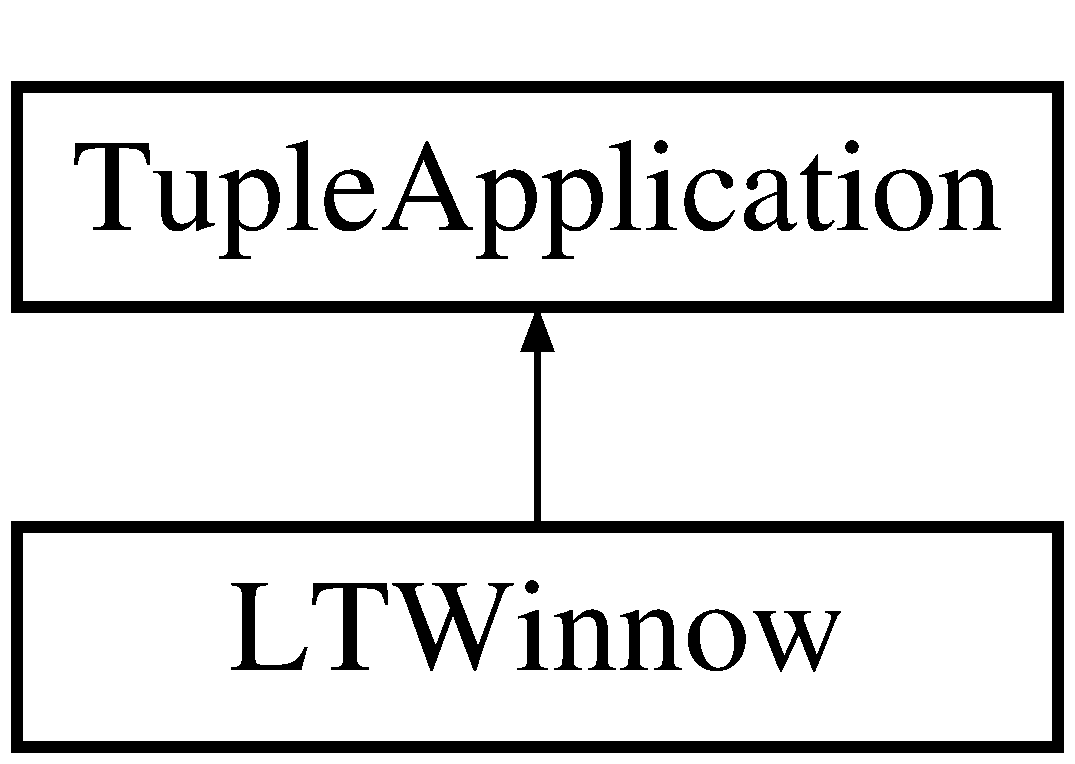
\includegraphics[height=2cm]{class_l_t_winnow}
\end{center}
\end{figure}
\subsection*{Protected Member Functions}
\begin{CompactItemize}
\item 
void \hyperlink{class_l_t_winnow_ec961ab4e19c71b475903972111c20e9}{consumeInput} ()
\item 
void \hyperlink{class_l_t_winnow_472d0a232050f4674339029b1aa47531}{work} ()
\item 
void \hyperlink{class_l_t_winnow_865de8a240ae781c8cc5567082edc2ea}{produceOutput} ()
\item 
\hyperlink{class_point}{Point} \hyperlink{class_l_t_winnow_768a5ced06ddfce6752be6cff4949500}{nextWeightedPoint} (\hyperlink{cowichan_8hpp_c96945095fd0ce7186a1d00a89f77d2c}{INT\_\-TYPE} $\ast$order)
\end{CompactItemize}
\subsection*{Static Protected Attributes}
\begin{CompactItemize}
\item 
static const char $\ast$ \hyperlink{class_l_t_winnow_9a64120d24bd1be307729b3ab560053c}{SYNCH\_\-LOCK} = \char`\"{}winnow synchronization lock\char`\"{}
\item 
static const char $\ast$ \hyperlink{class_l_t_winnow_5e608a12be3c5b85d3bf7d20aff67be7}{REQUEST} = \char`\"{}winnow request\char`\"{}
\item 
static const char $\ast$ \hyperlink{class_l_t_winnow_39f42512128fc000cd417bc0b36c659c}{WEIGHTED\_\-POINT} = \char`\"{}winnow weighted point\char`\"{}
\item 
static const char $\ast$ \hyperlink{class_l_t_winnow_f975efec2812f3c4f675fa8ac867b2a0}{COUNT} = \char`\"{}winnow number of points\char`\"{}
\item 
static const char $\ast$ \hyperlink{class_l_t_winnow_63e05f9d6b31574d30008155947682b7}{ROWS\_\-DONE} = \char`\"{}winnow rows reporting\char`\"{}
\end{CompactItemize}


\subsection{Detailed Description}
Performs the weighted point selection in tuple space. Uses a property of tuple-space which means no sorting needs to occur! 

\subsection{Member Function Documentation}
\hypertarget{class_l_t_winnow_ec961ab4e19c71b475903972111c20e9}{
\index{LTWinnow@{LTWinnow}!consumeInput@{consumeInput}}
\index{consumeInput@{consumeInput}!LTWinnow@{LTWinnow}}
\subsubsection[{consumeInput}]{\setlength{\rightskip}{0pt plus 5cm}void LTWinnow::consumeInput ()\hspace{0.3cm}{\tt  \mbox{[}protected, virtual\mbox{]}}}}
\label{class_l_t_winnow_ec961ab4e19c71b475903972111c20e9}


The consume input process is spawned once and should distribute tasks to the worker processes. 

Implements \hyperlink{class_tuple_application_e163c5a536de01c8b94b49528a17dab2}{TupleApplication}.\hypertarget{class_l_t_winnow_768a5ced06ddfce6752be6cff4949500}{
\index{LTWinnow@{LTWinnow}!nextWeightedPoint@{nextWeightedPoint}}
\index{nextWeightedPoint@{nextWeightedPoint}!LTWinnow@{LTWinnow}}
\subsubsection[{nextWeightedPoint}]{\setlength{\rightskip}{0pt plus 5cm}{\bf Point} LTWinnow::nextWeightedPoint ({\bf INT\_\-TYPE} $\ast$ {\em order})\hspace{0.3cm}{\tt  \mbox{[}protected\mbox{]}}}}
\label{class_l_t_winnow_768a5ced06ddfce6752be6cff4949500}


Figure out the next point we can pull out of tuple space. \begin{Desc}
\item[Parameters:]
\begin{description}
\item[{\em order}]the weight of the next point to pull out. \end{description}
\end{Desc}
\begin{Desc}
\item[Returns:]the point with the smallest weight w such that w $>$= order. \end{Desc}
\hypertarget{class_l_t_winnow_865de8a240ae781c8cc5567082edc2ea}{
\index{LTWinnow@{LTWinnow}!produceOutput@{produceOutput}}
\index{produceOutput@{produceOutput}!LTWinnow@{LTWinnow}}
\subsubsection[{produceOutput}]{\setlength{\rightskip}{0pt plus 5cm}void LTWinnow::produceOutput ()\hspace{0.3cm}{\tt  \mbox{[}protected, virtual\mbox{]}}}}
\label{class_l_t_winnow_865de8a240ae781c8cc5567082edc2ea}


The output producer decides when the tuple application is finished; once this function returns, the tuple application is complete. 

Implements \hyperlink{class_tuple_application_8743dfcf17dedd52887c0b2ab170d8dc}{TupleApplication}.\hypertarget{class_l_t_winnow_472d0a232050f4674339029b1aa47531}{
\index{LTWinnow@{LTWinnow}!work@{work}}
\index{work@{work}!LTWinnow@{LTWinnow}}
\subsubsection[{work}]{\setlength{\rightskip}{0pt plus 5cm}void LTWinnow::work ()\hspace{0.3cm}{\tt  \mbox{[}protected, virtual\mbox{]}}}}
\label{class_l_t_winnow_472d0a232050f4674339029b1aa47531}


Worker processes are created and killed after the output process has finished. 

Implements \hyperlink{class_tuple_application_ef6ae8bb1d697e4ed038b43320183c89}{TupleApplication}.

\subsection{Member Data Documentation}
\hypertarget{class_l_t_winnow_f975efec2812f3c4f675fa8ac867b2a0}{
\index{LTWinnow@{LTWinnow}!COUNT@{COUNT}}
\index{COUNT@{COUNT}!LTWinnow@{LTWinnow}}
\subsubsection[{COUNT}]{\setlength{\rightskip}{0pt plus 5cm}const char $\ast$ {\bf LTWinnow::COUNT} = \char`\"{}winnow number of points\char`\"{}\hspace{0.3cm}{\tt  \mbox{[}static, protected\mbox{]}}}}
\label{class_l_t_winnow_f975efec2812f3c4f675fa8ac867b2a0}


The number of weighted points in the tuple space. \hypertarget{class_l_t_winnow_5e608a12be3c5b85d3bf7d20aff67be7}{
\index{LTWinnow@{LTWinnow}!REQUEST@{REQUEST}}
\index{REQUEST@{REQUEST}!LTWinnow@{LTWinnow}}
\subsubsection[{REQUEST}]{\setlength{\rightskip}{0pt plus 5cm}const char $\ast$ {\bf LTWinnow::REQUEST} = \char`\"{}winnow request\char`\"{}\hspace{0.3cm}{\tt  \mbox{[}static, protected\mbox{]}}}}
\label{class_l_t_winnow_5e608a12be3c5b85d3bf7d20aff67be7}


Request to perform computation on a matrix row. \hypertarget{class_l_t_winnow_63e05f9d6b31574d30008155947682b7}{
\index{LTWinnow@{LTWinnow}!ROWS\_\-DONE@{ROWS\_\-DONE}}
\index{ROWS\_\-DONE@{ROWS\_\-DONE}!LTWinnow@{LTWinnow}}
\subsubsection[{ROWS\_\-DONE}]{\setlength{\rightskip}{0pt plus 5cm}const char $\ast$ {\bf LTWinnow::ROWS\_\-DONE} = \char`\"{}winnow rows reporting\char`\"{}\hspace{0.3cm}{\tt  \mbox{[}static, protected\mbox{]}}}}
\label{class_l_t_winnow_63e05f9d6b31574d30008155947682b7}


The number of rows that have had their computation finish. \hypertarget{class_l_t_winnow_9a64120d24bd1be307729b3ab560053c}{
\index{LTWinnow@{LTWinnow}!SYNCH\_\-LOCK@{SYNCH\_\-LOCK}}
\index{SYNCH\_\-LOCK@{SYNCH\_\-LOCK}!LTWinnow@{LTWinnow}}
\subsubsection[{SYNCH\_\-LOCK}]{\setlength{\rightskip}{0pt plus 5cm}const char $\ast$ {\bf LTWinnow::SYNCH\_\-LOCK} = \char`\"{}winnow synchronization lock\char`\"{}\hspace{0.3cm}{\tt  \mbox{[}static, protected\mbox{]}}}}
\label{class_l_t_winnow_9a64120d24bd1be307729b3ab560053c}


Synchronization lock (critical section). \hypertarget{class_l_t_winnow_39f42512128fc000cd417bc0b36c659c}{
\index{LTWinnow@{LTWinnow}!WEIGHTED\_\-POINT@{WEIGHTED\_\-POINT}}
\index{WEIGHTED\_\-POINT@{WEIGHTED\_\-POINT}!LTWinnow@{LTWinnow}}
\subsubsection[{WEIGHTED\_\-POINT}]{\setlength{\rightskip}{0pt plus 5cm}const char $\ast$ {\bf LTWinnow::WEIGHTED\_\-POINT} = \char`\"{}winnow weighted point\char`\"{}\hspace{0.3cm}{\tt  \mbox{[}static, protected\mbox{]}}}}
\label{class_l_t_winnow_39f42512128fc000cd417bc0b36c659c}


A weighted point in the tuple space. 

The documentation for this class was generated from the following files:\begin{CompactItemize}
\item 
cowichan\_\-lt/src/\hyperlink{winnow_8hpp}{winnow.hpp}\item 
cowichan\_\-lt/src/\hyperlink{cowichan__lt_2src_2winnow_8cpp}{winnow.cpp}\end{CompactItemize}

\hypertarget{classcowichan__tbb_1_1_make_dominant}{
\section{cowichan\_\-tbb::MakeDominant Class Reference}
\label{classcowichan__tbb_1_1_make_dominant}\index{cowichan\_\-tbb::MakeDominant@{cowichan\_\-tbb::MakeDominant}}
}
Makes a given matrix diagonally dominant.  


\subsection*{Public Member Functions}
\begin{CompactItemize}
\item 
\hyperlink{classcowichan__tbb_1_1_make_dominant_aa60cc1c8e84d1adedf84c4195bd94e6}{MakeDominant} (\hyperlink{cowichan_8hpp_3fb46f939e55c239fbc95656fc0f3399}{Matrix} matrix, \hyperlink{cowichan_8hpp_5b04577d5d21124855deaad298595371}{index\_\-t} \hyperlink{classcowichan__tbb_1_1_make_dominant_f329b8d7d34fe420ba91e124299629a5}{n}, \hyperlink{cowichan_8hpp_4d521b2c54a1f6312cc8fa04827eaf98}{real} \hyperlink{classcowichan__tbb_1_1_make_dominant_f47a49461fbef3e69bdb3c3f8fce66f3}{value})
\item 
void \hyperlink{classcowichan__tbb_1_1_make_dominant_55f09191fc150a1570c3cc29d7181416}{operator()} (const \hyperlink{cowichan__tbb_8hpp_8e2057f725b08f3a15513c378a453a47}{Range} \&rows) const 
\end{CompactItemize}
\subsection*{Private Attributes}
\begin{CompactItemize}
\item 
\hyperlink{cowichan_8hpp_3fb46f939e55c239fbc95656fc0f3399}{Matrix} \hyperlink{classcowichan__tbb_1_1_make_dominant_1d0d71f5d927d434b36149a7b0f4938c}{\_\-matrix}
\item 
\hyperlink{cowichan_8hpp_5b04577d5d21124855deaad298595371}{index\_\-t} \hyperlink{classcowichan__tbb_1_1_make_dominant_f329b8d7d34fe420ba91e124299629a5}{n}
\item 
const \hyperlink{cowichan_8hpp_4d521b2c54a1f6312cc8fa04827eaf98}{real} \hyperlink{classcowichan__tbb_1_1_make_dominant_f47a49461fbef3e69bdb3c3f8fce66f3}{value}
\end{CompactItemize}


\subsection{Detailed Description}
Makes a given matrix diagonally dominant. 

Modifies its diagonal elements. 

\subsection{Constructor \& Destructor Documentation}
\hypertarget{classcowichan__tbb_1_1_make_dominant_aa60cc1c8e84d1adedf84c4195bd94e6}{
\index{cowichan\_\-tbb::MakeDominant@{cowichan\_\-tbb::MakeDominant}!MakeDominant@{MakeDominant}}
\index{MakeDominant@{MakeDominant}!cowichan_tbb::MakeDominant@{cowichan\_\-tbb::MakeDominant}}
\subsubsection[{MakeDominant}]{\setlength{\rightskip}{0pt plus 5cm}cowichan\_\-tbb::MakeDominant::MakeDominant ({\bf Matrix} {\em matrix}, \/  {\bf index\_\-t} {\em n}, \/  {\bf real} {\em value})\hspace{0.3cm}{\tt  \mbox{[}inline\mbox{]}}}}
\label{classcowichan__tbb_1_1_make_dominant_aa60cc1c8e84d1adedf84c4195bd94e6}


Construct a make dominant object. \begin{Desc}
\item[Parameters:]
\begin{description}
\item[{\em matrix}]matrix to modify. \item[{\em n}]matrix size. \item[{\em value}]value for diagonal. \end{description}
\end{Desc}


\subsection{Member Function Documentation}
\hypertarget{classcowichan__tbb_1_1_make_dominant_55f09191fc150a1570c3cc29d7181416}{
\index{cowichan\_\-tbb::MakeDominant@{cowichan\_\-tbb::MakeDominant}!operator()@{operator()}}
\index{operator()@{operator()}!cowichan_tbb::MakeDominant@{cowichan\_\-tbb::MakeDominant}}
\subsubsection[{operator()}]{\setlength{\rightskip}{0pt plus 5cm}void cowichan\_\-tbb::MakeDominant::operator() (const {\bf Range} \& {\em rows}) const\hspace{0.3cm}{\tt  \mbox{[}inline\mbox{]}}}}
\label{classcowichan__tbb_1_1_make_dominant_55f09191fc150a1570c3cc29d7181416}


Sets diagonal elements to a given constant. \begin{Desc}
\item[Parameters:]
\begin{description}
\item[{\em rows}]range of rows to work on. \end{description}
\end{Desc}


\subsection{Member Data Documentation}
\hypertarget{classcowichan__tbb_1_1_make_dominant_1d0d71f5d927d434b36149a7b0f4938c}{
\index{cowichan\_\-tbb::MakeDominant@{cowichan\_\-tbb::MakeDominant}!\_\-matrix@{\_\-matrix}}
\index{\_\-matrix@{\_\-matrix}!cowichan_tbb::MakeDominant@{cowichan\_\-tbb::MakeDominant}}
\subsubsection[{\_\-matrix}]{\setlength{\rightskip}{0pt plus 5cm}{\bf Matrix} {\bf cowichan\_\-tbb::MakeDominant::\_\-matrix}\hspace{0.3cm}{\tt  \mbox{[}private\mbox{]}}}}
\label{classcowichan__tbb_1_1_make_dominant_1d0d71f5d927d434b36149a7b0f4938c}


Matrix to modify. \hypertarget{classcowichan__tbb_1_1_make_dominant_f329b8d7d34fe420ba91e124299629a5}{
\index{cowichan\_\-tbb::MakeDominant@{cowichan\_\-tbb::MakeDominant}!n@{n}}
\index{n@{n}!cowichan_tbb::MakeDominant@{cowichan\_\-tbb::MakeDominant}}
\subsubsection[{n}]{\setlength{\rightskip}{0pt plus 5cm}{\bf index\_\-t} {\bf cowichan\_\-tbb::MakeDominant::n}\hspace{0.3cm}{\tt  \mbox{[}private\mbox{]}}}}
\label{classcowichan__tbb_1_1_make_dominant_f329b8d7d34fe420ba91e124299629a5}


Matrix size. \hypertarget{classcowichan__tbb_1_1_make_dominant_f47a49461fbef3e69bdb3c3f8fce66f3}{
\index{cowichan\_\-tbb::MakeDominant@{cowichan\_\-tbb::MakeDominant}!value@{value}}
\index{value@{value}!cowichan_tbb::MakeDominant@{cowichan\_\-tbb::MakeDominant}}
\subsubsection[{value}]{\setlength{\rightskip}{0pt plus 5cm}const {\bf real} {\bf cowichan\_\-tbb::MakeDominant::value}\hspace{0.3cm}{\tt  \mbox{[}private\mbox{]}}}}
\label{classcowichan__tbb_1_1_make_dominant_f47a49461fbef3e69bdb3c3f8fce66f3}


Value to use for diagonal. 

The documentation for this class was generated from the following file:\begin{CompactItemize}
\item 
cowichan\_\-tbb/\hyperlink{cowichan__tbb_2outer_8cpp}{outer.cpp}\end{CompactItemize}

\hypertarget{classcowichan__tbb_1_1_mandelbrot}{
\section{cowichan\_\-tbb::Mandelbrot Class Reference}
\label{classcowichan__tbb_1_1_mandelbrot}\index{cowichan\_\-tbb::Mandelbrot@{cowichan\_\-tbb::Mandelbrot}}
}
Perform mandelbrot generation.  


\subsection*{Public Member Functions}
\begin{CompactItemize}
\item 
\hyperlink{classcowichan__tbb_1_1_mandelbrot_2bfef0a80393e6547fb979f1d2135de6}{Mandelbrot} (\hyperlink{cowichan_8hpp_82321152ddeeefe9c61350a42ed9e7af}{IntMatrix} matrix, \hyperlink{cowichan_8hpp_5b04577d5d21124855deaad298595371}{index\_\-t} \hyperlink{classcowichan__tbb_1_1_mandelbrot_698768b13a40cbab1410a4e162d1e450}{nr}, \hyperlink{cowichan_8hpp_5b04577d5d21124855deaad298595371}{index\_\-t} \hyperlink{classcowichan__tbb_1_1_mandelbrot_6eed478f27f441f57438392515f0f575}{nc}, \hyperlink{cowichan_8hpp_4d521b2c54a1f6312cc8fa04827eaf98}{real} x, \hyperlink{cowichan_8hpp_4d521b2c54a1f6312cc8fa04827eaf98}{real} y, \hyperlink{cowichan_8hpp_4d521b2c54a1f6312cc8fa04827eaf98}{real} width, \hyperlink{cowichan_8hpp_4d521b2c54a1f6312cc8fa04827eaf98}{real} height)
\item 
void \hyperlink{classcowichan__tbb_1_1_mandelbrot_5c8093ee0a5690df3260109e03174f97}{operator()} (const \hyperlink{cowichan__tbb_8hpp_e591b8e6980ddc5982ee22655da2ab8e}{Range2D} \&range) const 
\end{CompactItemize}
\subsection*{Private Member Functions}
\begin{CompactItemize}
\item 
\hyperlink{cowichan_8hpp_c96945095fd0ce7186a1d00a89f77d2c}{INT\_\-TYPE} \hyperlink{classcowichan__tbb_1_1_mandelbrot_12f71733227567ee4519921eb42e505b}{mandelCalc} (\hyperlink{cowichan_8hpp_4d521b2c54a1f6312cc8fa04827eaf98}{real} x, \hyperlink{cowichan_8hpp_4d521b2c54a1f6312cc8fa04827eaf98}{real} y) const 
\end{CompactItemize}
\subsection*{Private Attributes}
\begin{CompactItemize}
\item 
\hyperlink{cowichan_8hpp_82321152ddeeefe9c61350a42ed9e7af}{IntMatrix} \hyperlink{classcowichan__tbb_1_1_mandelbrot_640971f00a9b5d3697efbe8b9a45a56c}{\_\-matrix}
\item 
\hyperlink{cowichan_8hpp_5b04577d5d21124855deaad298595371}{index\_\-t} \hyperlink{classcowichan__tbb_1_1_mandelbrot_698768b13a40cbab1410a4e162d1e450}{nr}
\item 
\hyperlink{cowichan_8hpp_5b04577d5d21124855deaad298595371}{index\_\-t} \hyperlink{classcowichan__tbb_1_1_mandelbrot_6eed478f27f441f57438392515f0f575}{nc}
\item 
\hyperlink{cowichan_8hpp_4d521b2c54a1f6312cc8fa04827eaf98}{real} \hyperlink{classcowichan__tbb_1_1_mandelbrot_f67b1fd96e5e4aecd37d5357f89770ed}{baseX}
\item 
\hyperlink{cowichan_8hpp_4d521b2c54a1f6312cc8fa04827eaf98}{real} \hyperlink{classcowichan__tbb_1_1_mandelbrot_0e35b59f83677269cec9b40812c97d3c}{baseY}
\item 
\hyperlink{cowichan_8hpp_4d521b2c54a1f6312cc8fa04827eaf98}{real} \hyperlink{classcowichan__tbb_1_1_mandelbrot_cbe2697988d27d656dcb12fcf06674c7}{dX}
\item 
\hyperlink{cowichan_8hpp_4d521b2c54a1f6312cc8fa04827eaf98}{real} \hyperlink{classcowichan__tbb_1_1_mandelbrot_8fc166fc3009c058ef4b6582755f5f52}{dY}
\end{CompactItemize}


\subsection{Detailed Description}
Perform mandelbrot generation. 

\subsection{Constructor \& Destructor Documentation}
\hypertarget{classcowichan__tbb_1_1_mandelbrot_2bfef0a80393e6547fb979f1d2135de6}{
\index{cowichan\_\-tbb::Mandelbrot@{cowichan\_\-tbb::Mandelbrot}!Mandelbrot@{Mandelbrot}}
\index{Mandelbrot@{Mandelbrot}!cowichan_tbb::Mandelbrot@{cowichan\_\-tbb::Mandelbrot}}
\subsubsection[{Mandelbrot}]{\setlength{\rightskip}{0pt plus 5cm}cowichan\_\-tbb::Mandelbrot::Mandelbrot ({\bf IntMatrix} {\em matrix}, \/  {\bf index\_\-t} {\em nr}, \/  {\bf index\_\-t} {\em nc}, \/  {\bf real} {\em x}, \/  {\bf real} {\em y}, \/  {\bf real} {\em width}, \/  {\bf real} {\em height})\hspace{0.3cm}{\tt  \mbox{[}inline\mbox{]}}}}
\label{classcowichan__tbb_1_1_mandelbrot_2bfef0a80393e6547fb979f1d2135de6}


Construct a mandelbrot generation object. \begin{Desc}
\item[Parameters:]
\begin{description}
\item[{\em matrix}]matrix to fill. \item[{\em nr}]number of rows. \item[{\em nc}]number of columns. \item[{\em x}]base x. \item[{\em y}]base y. \item[{\em width}]width. \item[{\em height}]height. \end{description}
\end{Desc}


\subsection{Member Function Documentation}
\hypertarget{classcowichan__tbb_1_1_mandelbrot_12f71733227567ee4519921eb42e505b}{
\index{cowichan\_\-tbb::Mandelbrot@{cowichan\_\-tbb::Mandelbrot}!mandelCalc@{mandelCalc}}
\index{mandelCalc@{mandelCalc}!cowichan_tbb::Mandelbrot@{cowichan\_\-tbb::Mandelbrot}}
\subsubsection[{mandelCalc}]{\setlength{\rightskip}{0pt plus 5cm}{\bf INT\_\-TYPE} cowichan\_\-tbb::Mandelbrot::mandelCalc ({\bf real} {\em x}, \/  {\bf real} {\em y}) const\hspace{0.3cm}{\tt  \mbox{[}inline, private\mbox{]}}}}
\label{classcowichan__tbb_1_1_mandelbrot_12f71733227567ee4519921eb42e505b}


Performs the mandelbrot value calculation. \begin{Desc}
\item[Parameters:]
\begin{description}
\item[{\em x}]x-coordinate. \item[{\em y}]y-coordinate. \end{description}
\end{Desc}
\hypertarget{classcowichan__tbb_1_1_mandelbrot_5c8093ee0a5690df3260109e03174f97}{
\index{cowichan\_\-tbb::Mandelbrot@{cowichan\_\-tbb::Mandelbrot}!operator()@{operator()}}
\index{operator()@{operator()}!cowichan_tbb::Mandelbrot@{cowichan\_\-tbb::Mandelbrot}}
\subsubsection[{operator()}]{\setlength{\rightskip}{0pt plus 5cm}void cowichan\_\-tbb::Mandelbrot::operator() (const {\bf Range2D} \& {\em range}) const\hspace{0.3cm}{\tt  \mbox{[}inline\mbox{]}}}}
\label{classcowichan__tbb_1_1_mandelbrot_5c8093ee0a5690df3260109e03174f97}


Calculates a given portion of the current mandelbrot set \char`\"{}window\char`\"{}. \begin{Desc}
\item[Parameters:]
\begin{description}
\item[{\em range}]two-dimensional range. \end{description}
\end{Desc}


\subsection{Member Data Documentation}
\hypertarget{classcowichan__tbb_1_1_mandelbrot_640971f00a9b5d3697efbe8b9a45a56c}{
\index{cowichan\_\-tbb::Mandelbrot@{cowichan\_\-tbb::Mandelbrot}!\_\-matrix@{\_\-matrix}}
\index{\_\-matrix@{\_\-matrix}!cowichan_tbb::Mandelbrot@{cowichan\_\-tbb::Mandelbrot}}
\subsubsection[{\_\-matrix}]{\setlength{\rightskip}{0pt plus 5cm}{\bf IntMatrix} {\bf cowichan\_\-tbb::Mandelbrot::\_\-matrix}\hspace{0.3cm}{\tt  \mbox{[}private\mbox{]}}}}
\label{classcowichan__tbb_1_1_mandelbrot_640971f00a9b5d3697efbe8b9a45a56c}


Matrix. \hypertarget{classcowichan__tbb_1_1_mandelbrot_f67b1fd96e5e4aecd37d5357f89770ed}{
\index{cowichan\_\-tbb::Mandelbrot@{cowichan\_\-tbb::Mandelbrot}!baseX@{baseX}}
\index{baseX@{baseX}!cowichan_tbb::Mandelbrot@{cowichan\_\-tbb::Mandelbrot}}
\subsubsection[{baseX}]{\setlength{\rightskip}{0pt plus 5cm}{\bf real} {\bf cowichan\_\-tbb::Mandelbrot::baseX}\hspace{0.3cm}{\tt  \mbox{[}private\mbox{]}}}}
\label{classcowichan__tbb_1_1_mandelbrot_f67b1fd96e5e4aecd37d5357f89770ed}


x-coordinate of the lower left corner. \hypertarget{classcowichan__tbb_1_1_mandelbrot_0e35b59f83677269cec9b40812c97d3c}{
\index{cowichan\_\-tbb::Mandelbrot@{cowichan\_\-tbb::Mandelbrot}!baseY@{baseY}}
\index{baseY@{baseY}!cowichan_tbb::Mandelbrot@{cowichan\_\-tbb::Mandelbrot}}
\subsubsection[{baseY}]{\setlength{\rightskip}{0pt plus 5cm}{\bf real} {\bf cowichan\_\-tbb::Mandelbrot::baseY}\hspace{0.3cm}{\tt  \mbox{[}private\mbox{]}}}}
\label{classcowichan__tbb_1_1_mandelbrot_0e35b59f83677269cec9b40812c97d3c}


y-coordinate of the lower left corner. \hypertarget{classcowichan__tbb_1_1_mandelbrot_cbe2697988d27d656dcb12fcf06674c7}{
\index{cowichan\_\-tbb::Mandelbrot@{cowichan\_\-tbb::Mandelbrot}!dX@{dX}}
\index{dX@{dX}!cowichan_tbb::Mandelbrot@{cowichan\_\-tbb::Mandelbrot}}
\subsubsection[{dX}]{\setlength{\rightskip}{0pt plus 5cm}{\bf real} {\bf cowichan\_\-tbb::Mandelbrot::dX}\hspace{0.3cm}{\tt  \mbox{[}private\mbox{]}}}}
\label{classcowichan__tbb_1_1_mandelbrot_cbe2697988d27d656dcb12fcf06674c7}


Extent of the region along the x axis. \hypertarget{classcowichan__tbb_1_1_mandelbrot_8fc166fc3009c058ef4b6582755f5f52}{
\index{cowichan\_\-tbb::Mandelbrot@{cowichan\_\-tbb::Mandelbrot}!dY@{dY}}
\index{dY@{dY}!cowichan_tbb::Mandelbrot@{cowichan\_\-tbb::Mandelbrot}}
\subsubsection[{dY}]{\setlength{\rightskip}{0pt plus 5cm}{\bf real} {\bf cowichan\_\-tbb::Mandelbrot::dY}\hspace{0.3cm}{\tt  \mbox{[}private\mbox{]}}}}
\label{classcowichan__tbb_1_1_mandelbrot_8fc166fc3009c058ef4b6582755f5f52}


Extent of the region along the y axis. \hypertarget{classcowichan__tbb_1_1_mandelbrot_6eed478f27f441f57438392515f0f575}{
\index{cowichan\_\-tbb::Mandelbrot@{cowichan\_\-tbb::Mandelbrot}!nc@{nc}}
\index{nc@{nc}!cowichan_tbb::Mandelbrot@{cowichan\_\-tbb::Mandelbrot}}
\subsubsection[{nc}]{\setlength{\rightskip}{0pt plus 5cm}{\bf index\_\-t} {\bf cowichan\_\-tbb::Mandelbrot::nc}\hspace{0.3cm}{\tt  \mbox{[}private\mbox{]}}}}
\label{classcowichan__tbb_1_1_mandelbrot_6eed478f27f441f57438392515f0f575}


Number of columns in the matrix. \hypertarget{classcowichan__tbb_1_1_mandelbrot_698768b13a40cbab1410a4e162d1e450}{
\index{cowichan\_\-tbb::Mandelbrot@{cowichan\_\-tbb::Mandelbrot}!nr@{nr}}
\index{nr@{nr}!cowichan_tbb::Mandelbrot@{cowichan\_\-tbb::Mandelbrot}}
\subsubsection[{nr}]{\setlength{\rightskip}{0pt plus 5cm}{\bf index\_\-t} {\bf cowichan\_\-tbb::Mandelbrot::nr}\hspace{0.3cm}{\tt  \mbox{[}private\mbox{]}}}}
\label{classcowichan__tbb_1_1_mandelbrot_698768b13a40cbab1410a4e162d1e450}


Number of rows in the matrix. 

The documentation for this class was generated from the following file:\begin{CompactItemize}
\item 
cowichan\_\-tbb/\hyperlink{cowichan__tbb_2mandel_8cpp}{mandel.cpp}\end{CompactItemize}

\hypertarget{structcowichan__mpi_1_1maximum__cp}{
\section{cowichan\_\-mpi::maximum\_\-cp Struct Reference}
\label{structcowichan__mpi_1_1maximum__cp}\index{cowichan\_\-mpi::maximum\_\-cp@{cowichan\_\-mpi::maximum\_\-cp}}
}
\subsection*{Public Member Functions}
\begin{CompactItemize}
\item 
\hyperlink{structcowichan__mpi_1_1pt__cross}{pt\_\-cross} \hyperlink{structcowichan__mpi_1_1maximum__cp_4750f0e492fc75ebe72dc6238f48738a}{operator()} (\hyperlink{structcowichan__mpi_1_1pt__cross}{pt\_\-cross} a, \hyperlink{structcowichan__mpi_1_1pt__cross}{pt\_\-cross} b)
\end{CompactItemize}


\subsection{Detailed Description}
Reduction function for maximum cross point. 

\subsection{Member Function Documentation}
\hypertarget{structcowichan__mpi_1_1maximum__cp_4750f0e492fc75ebe72dc6238f48738a}{
\index{cowichan\_\-mpi::maximum\_\-cp@{cowichan\_\-mpi::maximum\_\-cp}!operator()@{operator()}}
\index{operator()@{operator()}!cowichan_mpi::maximum_cp@{cowichan\_\-mpi::maximum\_\-cp}}
\subsubsection[{operator()}]{\setlength{\rightskip}{0pt plus 5cm}{\bf pt\_\-cross} cowichan\_\-mpi::maximum\_\-cp::operator() ({\bf pt\_\-cross} {\em a}, \/  {\bf pt\_\-cross} {\em b})\hspace{0.3cm}{\tt  \mbox{[}inline\mbox{]}}}}
\label{structcowichan__mpi_1_1maximum__cp_4750f0e492fc75ebe72dc6238f48738a}


Get maximum cross point. \begin{Desc}
\item[Parameters:]
\begin{description}
\item[{\em a}]point 1. \item[{\em b}]point 2. \end{description}
\end{Desc}
\begin{Desc}
\item[Returns:]Maximum cross point. \end{Desc}


The documentation for this struct was generated from the following file:\begin{CompactItemize}
\item 
cowichan\_\-mpi/\hyperlink{cowichan__mpi_2hull_8cpp}{hull.cpp}\end{CompactItemize}

\hypertarget{structcowichan__mpi_1_1maximum__pt}{
\section{cowichan\_\-mpi::maximum\_\-pt Struct Reference}
\label{structcowichan__mpi_1_1maximum__pt}\index{cowichan\_\-mpi::maximum\_\-pt@{cowichan\_\-mpi::maximum\_\-pt}}
}
\subsection*{Public Member Functions}
\begin{CompactItemize}
\item 
\hyperlink{class_point}{Point} \hyperlink{structcowichan__mpi_1_1maximum__pt_abb641f4a48e373c2e0e7fd0b8f5d899}{operator()} (\hyperlink{class_point}{Point} a, \hyperlink{class_point}{Point} b)
\end{CompactItemize}


\subsection{Detailed Description}
MPI reduction primitive for calculating point maximum. 

\subsection{Member Function Documentation}
\hypertarget{structcowichan__mpi_1_1maximum__pt_abb641f4a48e373c2e0e7fd0b8f5d899}{
\index{cowichan\_\-mpi::maximum\_\-pt@{cowichan\_\-mpi::maximum\_\-pt}!operator()@{operator()}}
\index{operator()@{operator()}!cowichan_mpi::maximum_pt@{cowichan\_\-mpi::maximum\_\-pt}}
\subsubsection[{operator()}]{\setlength{\rightskip}{0pt plus 5cm}{\bf Point} cowichan\_\-mpi::maximum\_\-pt::operator() ({\bf Point} {\em a}, \/  {\bf Point} {\em b})\hspace{0.3cm}{\tt  \mbox{[}inline\mbox{]}}}}
\label{structcowichan__mpi_1_1maximum__pt_abb641f4a48e373c2e0e7fd0b8f5d899}


Get point maximum. \begin{Desc}
\item[Parameters:]
\begin{description}
\item[{\em a}]point 1. \item[{\em b}]point 2. \end{description}
\end{Desc}


The documentation for this struct was generated from the following file:\begin{CompactItemize}
\item 
cowichan\_\-mpi/\hyperlink{cowichan__mpi_2norm_8cpp}{norm.cpp}\end{CompactItemize}

\hypertarget{structcowichan__mpi_1_1maximum__x__pt}{
\section{cowichan\_\-mpi::maximum\_\-x\_\-pt Struct Reference}
\label{structcowichan__mpi_1_1maximum__x__pt}\index{cowichan\_\-mpi::maximum\_\-x\_\-pt@{cowichan\_\-mpi::maximum\_\-x\_\-pt}}
}
\subsection*{Public Member Functions}
\begin{CompactItemize}
\item 
\hyperlink{class_point}{Point} \hyperlink{structcowichan__mpi_1_1maximum__x__pt_a056f09712e6345f5425c11d52aaf466}{operator()} (\hyperlink{class_point}{Point} a, \hyperlink{class_point}{Point} b)
\end{CompactItemize}


\subsection{Detailed Description}
Reduction function for maximum x point. 

\subsection{Member Function Documentation}
\hypertarget{structcowichan__mpi_1_1maximum__x__pt_a056f09712e6345f5425c11d52aaf466}{
\index{cowichan\_\-mpi::maximum\_\-x\_\-pt@{cowichan\_\-mpi::maximum\_\-x\_\-pt}!operator()@{operator()}}
\index{operator()@{operator()}!cowichan_mpi::maximum_x_pt@{cowichan\_\-mpi::maximum\_\-x\_\-pt}}
\subsubsection[{operator()}]{\setlength{\rightskip}{0pt plus 5cm}{\bf Point} cowichan\_\-mpi::maximum\_\-x\_\-pt::operator() ({\bf Point} {\em a}, \/  {\bf Point} {\em b})\hspace{0.3cm}{\tt  \mbox{[}inline\mbox{]}}}}
\label{structcowichan__mpi_1_1maximum__x__pt_a056f09712e6345f5425c11d52aaf466}


Get maximum x point. \begin{Desc}
\item[Parameters:]
\begin{description}
\item[{\em a}]point 1. \item[{\em b}]point 2. \end{description}
\end{Desc}
\begin{Desc}
\item[Returns:]Maximum x point. \end{Desc}


The documentation for this struct was generated from the following file:\begin{CompactItemize}
\item 
cowichan\_\-mpi/\hyperlink{cowichan__mpi_2hull_8cpp}{hull.cpp}\end{CompactItemize}

\hypertarget{classcowichan__tbb_1_1_maximum_distance}{
\section{cowichan\_\-tbb::MaximumDistance Class Reference}
\label{classcowichan__tbb_1_1_maximum_distance}\index{cowichan\_\-tbb::MaximumDistance@{cowichan\_\-tbb::MaximumDistance}}
}
Compute maximum distance for hull.  


\subsection*{Public Member Functions}
\begin{CompactItemize}
\item 
\hyperlink{classcowichan__tbb_1_1_maximum_distance_27951c45e963c82338b89c8ca5f537a3}{MaximumDistance} (const \hyperlink{class_point}{PointVector} \&\hyperlink{classcowichan__tbb_1_1_maximum_distance_bc32ff1a7f0690db7e2bb11553406beb}{points}, const \hyperlink{class_point}{Point} \&\hyperlink{classcowichan__tbb_1_1_maximum_distance_f293990c96bce9deb63554e072ee8a72}{p1}, const \hyperlink{class_point}{Point} \&\hyperlink{classcowichan__tbb_1_1_maximum_distance_96e9aa3e660176029adbedbb147ca738}{p2})
\item 
\hyperlink{class_point}{Point} $\ast$ \hyperlink{classcowichan__tbb_1_1_maximum_distance_6c5d5b1704546428f6e38d82b3f395e0}{getPoint} () const 
\item 
\hyperlink{cowichan_8hpp_4d521b2c54a1f6312cc8fa04827eaf98}{real} \hyperlink{classcowichan__tbb_1_1_maximum_distance_e64a1737647520c65d563d5e0f3edc0c}{getDistance} () const 
\item 
void \hyperlink{classcowichan__tbb_1_1_maximum_distance_0f75c7ecaf6ed283b6b1b13cb65ae93c}{operator()} (const \hyperlink{cowichan__tbb_8hpp_8e2057f725b08f3a15513c378a453a47}{Range} \&range)
\item 
\hyperlink{classcowichan__tbb_1_1_maximum_distance_15452a15119559f5ef47b81921cd415d}{MaximumDistance} (\hyperlink{classcowichan__tbb_1_1_maximum_distance}{MaximumDistance} \&other, split)
\item 
void \hyperlink{classcowichan__tbb_1_1_maximum_distance_a786214cf1ab00a7bef0c8d7814ea2cb}{join} (const \hyperlink{classcowichan__tbb_1_1_maximum_distance}{MaximumDistance} \&other)
\end{CompactItemize}
\subsection*{Private Attributes}
\begin{CompactItemize}
\item 
const \hyperlink{class_point}{PointVector} \& \hyperlink{classcowichan__tbb_1_1_maximum_distance_bc32ff1a7f0690db7e2bb11553406beb}{points}
\item 
const \hyperlink{class_point}{Point} \& \hyperlink{classcowichan__tbb_1_1_maximum_distance_f293990c96bce9deb63554e072ee8a72}{p1}
\item 
const \hyperlink{class_point}{Point} \& \hyperlink{classcowichan__tbb_1_1_maximum_distance_96e9aa3e660176029adbedbb147ca738}{p2}
\item 
\hyperlink{class_point}{Point} $\ast$ \hyperlink{classcowichan__tbb_1_1_maximum_distance_b46579dadde304ad7fb7242076387e46}{maxPoint}
\item 
\hyperlink{cowichan_8hpp_4d521b2c54a1f6312cc8fa04827eaf98}{real} \hyperlink{classcowichan__tbb_1_1_maximum_distance_d5e6581f6e4956f9abf886d2dced0772}{maxCross}
\end{CompactItemize}


\subsection{Detailed Description}
Compute maximum distance for hull. 

Computes the maximum signed distance from a point to a line, given the line and list of points. 

\subsection{Constructor \& Destructor Documentation}
\hypertarget{classcowichan__tbb_1_1_maximum_distance_27951c45e963c82338b89c8ca5f537a3}{
\index{cowichan\_\-tbb::MaximumDistance@{cowichan\_\-tbb::MaximumDistance}!MaximumDistance@{MaximumDistance}}
\index{MaximumDistance@{MaximumDistance}!cowichan_tbb::MaximumDistance@{cowichan\_\-tbb::MaximumDistance}}
\subsubsection[{MaximumDistance}]{\setlength{\rightskip}{0pt plus 5cm}cowichan\_\-tbb::MaximumDistance::MaximumDistance (const {\bf PointVector} \& {\em points}, \/  const {\bf Point} \& {\em p1}, \/  const {\bf Point} \& {\em p2})\hspace{0.3cm}{\tt  \mbox{[}inline\mbox{]}}}}
\label{classcowichan__tbb_1_1_maximum_distance_27951c45e963c82338b89c8ca5f537a3}


Construct a maximum distance object. \begin{Desc}
\item[Parameters:]
\begin{description}
\item[{\em points}]points. \item[{\em p1}]first point forming the line. \item[{\em p2}]second point forming the line. \end{description}
\end{Desc}
\hypertarget{classcowichan__tbb_1_1_maximum_distance_15452a15119559f5ef47b81921cd415d}{
\index{cowichan\_\-tbb::MaximumDistance@{cowichan\_\-tbb::MaximumDistance}!MaximumDistance@{MaximumDistance}}
\index{MaximumDistance@{MaximumDistance}!cowichan_tbb::MaximumDistance@{cowichan\_\-tbb::MaximumDistance}}
\subsubsection[{MaximumDistance}]{\setlength{\rightskip}{0pt plus 5cm}cowichan\_\-tbb::MaximumDistance::MaximumDistance ({\bf MaximumDistance} \& {\em other}, \/  split)\hspace{0.3cm}{\tt  \mbox{[}inline\mbox{]}}}}
\label{classcowichan__tbb_1_1_maximum_distance_15452a15119559f5ef47b81921cd415d}


Splitting (TBB) constructor. \begin{Desc}
\item[Parameters:]
\begin{description}
\item[{\em other}]object to split. \end{description}
\end{Desc}


\subsection{Member Function Documentation}
\hypertarget{classcowichan__tbb_1_1_maximum_distance_e64a1737647520c65d563d5e0f3edc0c}{
\index{cowichan\_\-tbb::MaximumDistance@{cowichan\_\-tbb::MaximumDistance}!getDistance@{getDistance}}
\index{getDistance@{getDistance}!cowichan_tbb::MaximumDistance@{cowichan\_\-tbb::MaximumDistance}}
\subsubsection[{getDistance}]{\setlength{\rightskip}{0pt plus 5cm}{\bf real} cowichan\_\-tbb::MaximumDistance::getDistance () const\hspace{0.3cm}{\tt  \mbox{[}inline\mbox{]}}}}
\label{classcowichan__tbb_1_1_maximum_distance_e64a1737647520c65d563d5e0f3edc0c}


Gets the signed cross product to that point. \begin{Desc}
\item[Returns:]Max point cross product. \end{Desc}
\hypertarget{classcowichan__tbb_1_1_maximum_distance_6c5d5b1704546428f6e38d82b3f395e0}{
\index{cowichan\_\-tbb::MaximumDistance@{cowichan\_\-tbb::MaximumDistance}!getPoint@{getPoint}}
\index{getPoint@{getPoint}!cowichan_tbb::MaximumDistance@{cowichan\_\-tbb::MaximumDistance}}
\subsubsection[{getPoint}]{\setlength{\rightskip}{0pt plus 5cm}{\bf Point}$\ast$ cowichan\_\-tbb::MaximumDistance::getPoint () const\hspace{0.3cm}{\tt  \mbox{[}inline\mbox{]}}}}
\label{classcowichan__tbb_1_1_maximum_distance_6c5d5b1704546428f6e38d82b3f395e0}


Gets the point with maximum signed distance (if it has already been calculated). \begin{Desc}
\item[Returns:]Max distance point. \end{Desc}
\hypertarget{classcowichan__tbb_1_1_maximum_distance_a786214cf1ab00a7bef0c8d7814ea2cb}{
\index{cowichan\_\-tbb::MaximumDistance@{cowichan\_\-tbb::MaximumDistance}!join@{join}}
\index{join@{join}!cowichan_tbb::MaximumDistance@{cowichan\_\-tbb::MaximumDistance}}
\subsubsection[{join}]{\setlength{\rightskip}{0pt plus 5cm}void cowichan\_\-tbb::MaximumDistance::join (const {\bf MaximumDistance} \& {\em other})\hspace{0.3cm}{\tt  \mbox{[}inline\mbox{]}}}}
\label{classcowichan__tbb_1_1_maximum_distance_a786214cf1ab00a7bef0c8d7814ea2cb}


Joiner (TBB). \begin{Desc}
\item[Parameters:]
\begin{description}
\item[{\em other}]object to join. \end{description}
\end{Desc}
\hypertarget{classcowichan__tbb_1_1_maximum_distance_0f75c7ecaf6ed283b6b1b13cb65ae93c}{
\index{cowichan\_\-tbb::MaximumDistance@{cowichan\_\-tbb::MaximumDistance}!operator()@{operator()}}
\index{operator()@{operator()}!cowichan_tbb::MaximumDistance@{cowichan\_\-tbb::MaximumDistance}}
\subsubsection[{operator()}]{\setlength{\rightskip}{0pt plus 5cm}void cowichan\_\-tbb::MaximumDistance::operator() (const {\bf Range} \& {\em range})\hspace{0.3cm}{\tt  \mbox{[}inline\mbox{]}}}}
\label{classcowichan__tbb_1_1_maximum_distance_0f75c7ecaf6ed283b6b1b13cb65ae93c}


Calculates the \hyperlink{class_point}{Point} with maximum signed distance. \begin{Desc}
\item[Parameters:]
\begin{description}
\item[{\em range}]range of points to work on. \end{description}
\end{Desc}


\subsection{Member Data Documentation}
\hypertarget{classcowichan__tbb_1_1_maximum_distance_d5e6581f6e4956f9abf886d2dced0772}{
\index{cowichan\_\-tbb::MaximumDistance@{cowichan\_\-tbb::MaximumDistance}!maxCross@{maxCross}}
\index{maxCross@{maxCross}!cowichan_tbb::MaximumDistance@{cowichan\_\-tbb::MaximumDistance}}
\subsubsection[{maxCross}]{\setlength{\rightskip}{0pt plus 5cm}{\bf real} {\bf cowichan\_\-tbb::MaximumDistance::maxCross}\hspace{0.3cm}{\tt  \mbox{[}private\mbox{]}}}}
\label{classcowichan__tbb_1_1_maximum_distance_d5e6581f6e4956f9abf886d2dced0772}


Maximum cross product. \hypertarget{classcowichan__tbb_1_1_maximum_distance_b46579dadde304ad7fb7242076387e46}{
\index{cowichan\_\-tbb::MaximumDistance@{cowichan\_\-tbb::MaximumDistance}!maxPoint@{maxPoint}}
\index{maxPoint@{maxPoint}!cowichan_tbb::MaximumDistance@{cowichan\_\-tbb::MaximumDistance}}
\subsubsection[{maxPoint}]{\setlength{\rightskip}{0pt plus 5cm}{\bf Point}$\ast$ {\bf cowichan\_\-tbb::MaximumDistance::maxPoint}\hspace{0.3cm}{\tt  \mbox{[}private\mbox{]}}}}
\label{classcowichan__tbb_1_1_maximum_distance_b46579dadde304ad7fb7242076387e46}


\hyperlink{class_point}{Point} of maximum distance. \hypertarget{classcowichan__tbb_1_1_maximum_distance_f293990c96bce9deb63554e072ee8a72}{
\index{cowichan\_\-tbb::MaximumDistance@{cowichan\_\-tbb::MaximumDistance}!p1@{p1}}
\index{p1@{p1}!cowichan_tbb::MaximumDistance@{cowichan\_\-tbb::MaximumDistance}}
\subsubsection[{p1}]{\setlength{\rightskip}{0pt plus 5cm}const {\bf Point}\& {\bf cowichan\_\-tbb::MaximumDistance::p1}\hspace{0.3cm}{\tt  \mbox{[}private\mbox{]}}}}
\label{classcowichan__tbb_1_1_maximum_distance_f293990c96bce9deb63554e072ee8a72}


First point forming the line. \hypertarget{classcowichan__tbb_1_1_maximum_distance_96e9aa3e660176029adbedbb147ca738}{
\index{cowichan\_\-tbb::MaximumDistance@{cowichan\_\-tbb::MaximumDistance}!p2@{p2}}
\index{p2@{p2}!cowichan_tbb::MaximumDistance@{cowichan\_\-tbb::MaximumDistance}}
\subsubsection[{p2}]{\setlength{\rightskip}{0pt plus 5cm}const {\bf Point}\& {\bf cowichan\_\-tbb::MaximumDistance::p2}\hspace{0.3cm}{\tt  \mbox{[}private\mbox{]}}}}
\label{classcowichan__tbb_1_1_maximum_distance_96e9aa3e660176029adbedbb147ca738}


Second point forming the line. \hypertarget{classcowichan__tbb_1_1_maximum_distance_bc32ff1a7f0690db7e2bb11553406beb}{
\index{cowichan\_\-tbb::MaximumDistance@{cowichan\_\-tbb::MaximumDistance}!points@{points}}
\index{points@{points}!cowichan_tbb::MaximumDistance@{cowichan\_\-tbb::MaximumDistance}}
\subsubsection[{points}]{\setlength{\rightskip}{0pt plus 5cm}const {\bf PointVector}\& {\bf cowichan\_\-tbb::MaximumDistance::points}\hspace{0.3cm}{\tt  \mbox{[}private\mbox{]}}}}
\label{classcowichan__tbb_1_1_maximum_distance_bc32ff1a7f0690db7e2bb11553406beb}


Points. 

The documentation for this class was generated from the following file:\begin{CompactItemize}
\item 
cowichan\_\-tbb/\hyperlink{cowichan__tbb_2hull_8cpp}{hull.cpp}\end{CompactItemize}

\hypertarget{classcowichan__tbb_1_1_max_reducer}{
\section{cowichan\_\-tbb::MaxReducer Class Reference}
\label{classcowichan__tbb_1_1_max_reducer}\index{cowichan\_\-tbb::MaxReducer@{cowichan\_\-tbb::MaxReducer}}
}
Finds the maximum value in the image.  


\subsection*{Public Member Functions}
\begin{CompactItemize}
\item 
\hyperlink{classcowichan__tbb_1_1_max_reducer_040700219bf9b280323932d458116a53}{MaxReducer} (\hyperlink{cowichan_8hpp_82321152ddeeefe9c61350a42ed9e7af}{IntMatrix} image, \hyperlink{cowichan_8hpp_5b04577d5d21124855deaad298595371}{index\_\-t} \hyperlink{classcowichan__tbb_1_1_max_reducer_478817df677bfd5331c8a9a7f5e62de3}{nc})
\item 
\hyperlink{cowichan_8hpp_c96945095fd0ce7186a1d00a89f77d2c}{INT\_\-TYPE} \hyperlink{classcowichan__tbb_1_1_max_reducer_e4c54bf79d09499d4f91457a45a06a08}{getMaximum} () const 
\item 
void \hyperlink{classcowichan__tbb_1_1_max_reducer_a3ee1f93e3d1cf88da3669dfe73108f9}{operator()} (const \hyperlink{cowichan__tbb_8hpp_e591b8e6980ddc5982ee22655da2ab8e}{Range2D} \&range)
\item 
\hyperlink{classcowichan__tbb_1_1_max_reducer_df02ca92e3124c21671407a220a8081e}{MaxReducer} (\hyperlink{classcowichan__tbb_1_1_max_reducer}{MaxReducer} \&other, split)
\item 
void \hyperlink{classcowichan__tbb_1_1_max_reducer_ebeb8ee596f035a94d638b497135343b}{join} (const \hyperlink{classcowichan__tbb_1_1_max_reducer}{MaxReducer} \&other)
\end{CompactItemize}
\subsection*{Private Attributes}
\begin{CompactItemize}
\item 
\hyperlink{cowichan_8hpp_82321152ddeeefe9c61350a42ed9e7af}{IntMatrix} \hyperlink{classcowichan__tbb_1_1_max_reducer_f8ca766f2d3f828c10b03077e41f3a6b}{\_\-image}
\item 
\hyperlink{cowichan_8hpp_c96945095fd0ce7186a1d00a89f77d2c}{INT\_\-TYPE} \hyperlink{classcowichan__tbb_1_1_max_reducer_73c80dd6f6ded9d51b2c83e9a4a50501}{\_\-max}
\item 
const \hyperlink{cowichan_8hpp_5b04577d5d21124855deaad298595371}{index\_\-t} \hyperlink{classcowichan__tbb_1_1_max_reducer_478817df677bfd5331c8a9a7f5e62de3}{nc}
\end{CompactItemize}


\subsection{Detailed Description}
Finds the maximum value in the image. 

\subsection{Constructor \& Destructor Documentation}
\hypertarget{classcowichan__tbb_1_1_max_reducer_040700219bf9b280323932d458116a53}{
\index{cowichan\_\-tbb::MaxReducer@{cowichan\_\-tbb::MaxReducer}!MaxReducer@{MaxReducer}}
\index{MaxReducer@{MaxReducer}!cowichan_tbb::MaxReducer@{cowichan\_\-tbb::MaxReducer}}
\subsubsection[{MaxReducer}]{\setlength{\rightskip}{0pt plus 5cm}cowichan\_\-tbb::MaxReducer::MaxReducer ({\bf IntMatrix} {\em image}, \/  {\bf index\_\-t} {\em nc})\hspace{0.3cm}{\tt  \mbox{[}inline\mbox{]}}}}
\label{classcowichan__tbb_1_1_max_reducer_040700219bf9b280323932d458116a53}


Constructs a max reducer. Initialise max with the lowest possible value. \begin{Desc}
\item[Parameters:]
\begin{description}
\item[{\em image}]image matrix. \item[{\em nc}]number of matrix columns. \end{description}
\end{Desc}
\hypertarget{classcowichan__tbb_1_1_max_reducer_df02ca92e3124c21671407a220a8081e}{
\index{cowichan\_\-tbb::MaxReducer@{cowichan\_\-tbb::MaxReducer}!MaxReducer@{MaxReducer}}
\index{MaxReducer@{MaxReducer}!cowichan_tbb::MaxReducer@{cowichan\_\-tbb::MaxReducer}}
\subsubsection[{MaxReducer}]{\setlength{\rightskip}{0pt plus 5cm}cowichan\_\-tbb::MaxReducer::MaxReducer ({\bf MaxReducer} \& {\em other}, \/  split)\hspace{0.3cm}{\tt  \mbox{[}inline\mbox{]}}}}
\label{classcowichan__tbb_1_1_max_reducer_df02ca92e3124c21671407a220a8081e}


Splitting (TBB) constructor. \begin{Desc}
\item[Parameters:]
\begin{description}
\item[{\em other}]object to split. \end{description}
\end{Desc}


\subsection{Member Function Documentation}
\hypertarget{classcowichan__tbb_1_1_max_reducer_e4c54bf79d09499d4f91457a45a06a08}{
\index{cowichan\_\-tbb::MaxReducer@{cowichan\_\-tbb::MaxReducer}!getMaximum@{getMaximum}}
\index{getMaximum@{getMaximum}!cowichan_tbb::MaxReducer@{cowichan\_\-tbb::MaxReducer}}
\subsubsection[{getMaximum}]{\setlength{\rightskip}{0pt plus 5cm}{\bf INT\_\-TYPE} cowichan\_\-tbb::MaxReducer::getMaximum () const\hspace{0.3cm}{\tt  \mbox{[}inline\mbox{]}}}}
\label{classcowichan__tbb_1_1_max_reducer_e4c54bf79d09499d4f91457a45a06a08}


Get maximum value. \begin{Desc}
\item[Returns:]Maximum value. \end{Desc}
\hypertarget{classcowichan__tbb_1_1_max_reducer_ebeb8ee596f035a94d638b497135343b}{
\index{cowichan\_\-tbb::MaxReducer@{cowichan\_\-tbb::MaxReducer}!join@{join}}
\index{join@{join}!cowichan_tbb::MaxReducer@{cowichan\_\-tbb::MaxReducer}}
\subsubsection[{join}]{\setlength{\rightskip}{0pt plus 5cm}void cowichan\_\-tbb::MaxReducer::join (const {\bf MaxReducer} \& {\em other})\hspace{0.3cm}{\tt  \mbox{[}inline\mbox{]}}}}
\label{classcowichan__tbb_1_1_max_reducer_ebeb8ee596f035a94d638b497135343b}


Joiner (TBB). \begin{Desc}
\item[Parameters:]
\begin{description}
\item[{\em other}]object to join. \end{description}
\end{Desc}
\hypertarget{classcowichan__tbb_1_1_max_reducer_a3ee1f93e3d1cf88da3669dfe73108f9}{
\index{cowichan\_\-tbb::MaxReducer@{cowichan\_\-tbb::MaxReducer}!operator()@{operator()}}
\index{operator()@{operator()}!cowichan_tbb::MaxReducer@{cowichan\_\-tbb::MaxReducer}}
\subsubsection[{operator()}]{\setlength{\rightskip}{0pt plus 5cm}void cowichan\_\-tbb::MaxReducer::operator() (const {\bf Range2D} \& {\em range})\hspace{0.3cm}{\tt  \mbox{[}inline\mbox{]}}}}
\label{classcowichan__tbb_1_1_max_reducer_a3ee1f93e3d1cf88da3669dfe73108f9}


Calculates the maximum value over the given range. \begin{Desc}
\item[Parameters:]
\begin{description}
\item[{\em range}]row/column range. \end{description}
\end{Desc}


\subsection{Member Data Documentation}
\hypertarget{classcowichan__tbb_1_1_max_reducer_f8ca766f2d3f828c10b03077e41f3a6b}{
\index{cowichan\_\-tbb::MaxReducer@{cowichan\_\-tbb::MaxReducer}!\_\-image@{\_\-image}}
\index{\_\-image@{\_\-image}!cowichan_tbb::MaxReducer@{cowichan\_\-tbb::MaxReducer}}
\subsubsection[{\_\-image}]{\setlength{\rightskip}{0pt plus 5cm}{\bf IntMatrix} {\bf cowichan\_\-tbb::MaxReducer::\_\-image}\hspace{0.3cm}{\tt  \mbox{[}private\mbox{]}}}}
\label{classcowichan__tbb_1_1_max_reducer_f8ca766f2d3f828c10b03077e41f3a6b}


Image matrix. \hypertarget{classcowichan__tbb_1_1_max_reducer_73c80dd6f6ded9d51b2c83e9a4a50501}{
\index{cowichan\_\-tbb::MaxReducer@{cowichan\_\-tbb::MaxReducer}!\_\-max@{\_\-max}}
\index{\_\-max@{\_\-max}!cowichan_tbb::MaxReducer@{cowichan\_\-tbb::MaxReducer}}
\subsubsection[{\_\-max}]{\setlength{\rightskip}{0pt plus 5cm}{\bf INT\_\-TYPE} {\bf cowichan\_\-tbb::MaxReducer::\_\-max}\hspace{0.3cm}{\tt  \mbox{[}private\mbox{]}}}}
\label{classcowichan__tbb_1_1_max_reducer_73c80dd6f6ded9d51b2c83e9a4a50501}


Maximum value. \hypertarget{classcowichan__tbb_1_1_max_reducer_478817df677bfd5331c8a9a7f5e62de3}{
\index{cowichan\_\-tbb::MaxReducer@{cowichan\_\-tbb::MaxReducer}!nc@{nc}}
\index{nc@{nc}!cowichan_tbb::MaxReducer@{cowichan\_\-tbb::MaxReducer}}
\subsubsection[{nc}]{\setlength{\rightskip}{0pt plus 5cm}const {\bf index\_\-t} {\bf cowichan\_\-tbb::MaxReducer::nc}\hspace{0.3cm}{\tt  \mbox{[}private\mbox{]}}}}
\label{classcowichan__tbb_1_1_max_reducer_478817df677bfd5331c8a9a7f5e62de3}


Number of columns in the matrix. 

The documentation for this class was generated from the following file:\begin{CompactItemize}
\item 
cowichan\_\-tbb/\hyperlink{cowichan__tbb_2thresh_8cpp}{thresh.cpp}\end{CompactItemize}

\hypertarget{structcowichan__mpi_1_1minimum__pt}{
\section{cowichan\_\-mpi::minimum\_\-pt Struct Reference}
\label{structcowichan__mpi_1_1minimum__pt}\index{cowichan\_\-mpi::minimum\_\-pt@{cowichan\_\-mpi::minimum\_\-pt}}
}
\subsection*{Public Member Functions}
\begin{CompactItemize}
\item 
\hyperlink{class_point}{Point} \hyperlink{structcowichan__mpi_1_1minimum__pt_627215a36e3748e8ca0ff907a2a24f65}{operator()} (\hyperlink{class_point}{Point} a, \hyperlink{class_point}{Point} b)
\end{CompactItemize}


\subsection{Detailed Description}
MPI reduction primitive for calculating point minimum. 

\subsection{Member Function Documentation}
\hypertarget{structcowichan__mpi_1_1minimum__pt_627215a36e3748e8ca0ff907a2a24f65}{
\index{cowichan\_\-mpi::minimum\_\-pt@{cowichan\_\-mpi::minimum\_\-pt}!operator()@{operator()}}
\index{operator()@{operator()}!cowichan_mpi::minimum_pt@{cowichan\_\-mpi::minimum\_\-pt}}
\subsubsection[{operator()}]{\setlength{\rightskip}{0pt plus 5cm}{\bf Point} cowichan\_\-mpi::minimum\_\-pt::operator() ({\bf Point} {\em a}, \/  {\bf Point} {\em b})\hspace{0.3cm}{\tt  \mbox{[}inline\mbox{]}}}}
\label{structcowichan__mpi_1_1minimum__pt_627215a36e3748e8ca0ff907a2a24f65}


Get point minimum. \begin{Desc}
\item[Parameters:]
\begin{description}
\item[{\em a}]point 1. \item[{\em b}]point 2. \end{description}
\end{Desc}


The documentation for this struct was generated from the following file:\begin{CompactItemize}
\item 
cowichan\_\-mpi/\hyperlink{cowichan__mpi_2norm_8cpp}{norm.cpp}\end{CompactItemize}

\hypertarget{structcowichan__mpi_1_1minimum__x__pt}{
\section{cowichan\_\-mpi::minimum\_\-x\_\-pt Struct Reference}
\label{structcowichan__mpi_1_1minimum__x__pt}\index{cowichan\_\-mpi::minimum\_\-x\_\-pt@{cowichan\_\-mpi::minimum\_\-x\_\-pt}}
}
\subsection*{Public Member Functions}
\begin{CompactItemize}
\item 
\hyperlink{class_point}{Point} \hyperlink{structcowichan__mpi_1_1minimum__x__pt_64366aae9a252157bead8637d9b2ea8d}{operator()} (\hyperlink{class_point}{Point} a, \hyperlink{class_point}{Point} b)
\end{CompactItemize}


\subsection{Detailed Description}
Reduction function for minimum x point. 

\subsection{Member Function Documentation}
\hypertarget{structcowichan__mpi_1_1minimum__x__pt_64366aae9a252157bead8637d9b2ea8d}{
\index{cowichan\_\-mpi::minimum\_\-x\_\-pt@{cowichan\_\-mpi::minimum\_\-x\_\-pt}!operator()@{operator()}}
\index{operator()@{operator()}!cowichan_mpi::minimum_x_pt@{cowichan\_\-mpi::minimum\_\-x\_\-pt}}
\subsubsection[{operator()}]{\setlength{\rightskip}{0pt plus 5cm}{\bf Point} cowichan\_\-mpi::minimum\_\-x\_\-pt::operator() ({\bf Point} {\em a}, \/  {\bf Point} {\em b})\hspace{0.3cm}{\tt  \mbox{[}inline\mbox{]}}}}
\label{structcowichan__mpi_1_1minimum__x__pt_64366aae9a252157bead8637d9b2ea8d}


Get minimum x point. \begin{Desc}
\item[Parameters:]
\begin{description}
\item[{\em a}]point 1. \item[{\em b}]point 2. \end{description}
\end{Desc}
\begin{Desc}
\item[Returns:]Minimum x point. \end{Desc}


The documentation for this struct was generated from the following file:\begin{CompactItemize}
\item 
cowichan\_\-mpi/\hyperlink{cowichan__mpi_2hull_8cpp}{hull.cpp}\end{CompactItemize}

\hypertarget{classcowichan__tbb_1_1_min_max_reducer}{
\section{cowichan\_\-tbb::MinMaxReducer Class Reference}
\label{classcowichan__tbb_1_1_min_max_reducer}\index{cowichan\_\-tbb::MinMaxReducer@{cowichan\_\-tbb::MinMaxReducer}}
}
Performs the minimum and maximum reductions.  


\subsection*{Public Member Functions}
\begin{CompactItemize}
\item 
\hyperlink{classcowichan__tbb_1_1_min_max_reducer_29bbea72ee03400fad8cc9db152fda11}{MinMaxReducer} (\hyperlink{class_point}{PointVector} \hyperlink{classcowichan__tbb_1_1_min_max_reducer_40d6051859ad295c7e713ceb8c5ebf32}{pointsIn})
\item 
\hyperlink{class_point}{Point} \hyperlink{classcowichan__tbb_1_1_min_max_reducer_111be26690582d53727d4e091a8d2aa5}{getMinimum} () const 
\item 
\hyperlink{class_point}{Point} \hyperlink{classcowichan__tbb_1_1_min_max_reducer_71664616ef2ae1cfbd0f7aa0bee6c60f}{getMaximum} () const 
\item 
void \hyperlink{classcowichan__tbb_1_1_min_max_reducer_cb23bd9de26da84eb679dd03d123083d}{operator()} (const \hyperlink{cowichan__tbb_8hpp_8e2057f725b08f3a15513c378a453a47}{Range} \&range)
\item 
\hyperlink{classcowichan__tbb_1_1_min_max_reducer_ed85c930182f104ddac11d4814038e2d}{MinMaxReducer} (\hyperlink{classcowichan__tbb_1_1_min_max_reducer}{MinMaxReducer} \&other, split)
\item 
void \hyperlink{classcowichan__tbb_1_1_min_max_reducer_62cc9f7c40fedcd7f7306004b62932ff}{join} (const \hyperlink{classcowichan__tbb_1_1_min_max_reducer}{MinMaxReducer} \&other)
\end{CompactItemize}
\subsection*{Private Attributes}
\begin{CompactItemize}
\item 
\hyperlink{class_point}{PointVector} \hyperlink{classcowichan__tbb_1_1_min_max_reducer_40d6051859ad295c7e713ceb8c5ebf32}{pointsIn}
\item 
\hyperlink{class_point}{Point} \hyperlink{classcowichan__tbb_1_1_min_max_reducer_6445a2879ca5b7ca9d3c30d188fa3d6f}{minPoint}
\item 
\hyperlink{class_point}{Point} \hyperlink{classcowichan__tbb_1_1_min_max_reducer_0714c4e137e6df5122245fe6230f0aee}{maxPoint}
\end{CompactItemize}


\subsection{Detailed Description}
Performs the minimum and maximum reductions. 

\subsection{Constructor \& Destructor Documentation}
\hypertarget{classcowichan__tbb_1_1_min_max_reducer_29bbea72ee03400fad8cc9db152fda11}{
\index{cowichan\_\-tbb::MinMaxReducer@{cowichan\_\-tbb::MinMaxReducer}!MinMaxReducer@{MinMaxReducer}}
\index{MinMaxReducer@{MinMaxReducer}!cowichan_tbb::MinMaxReducer@{cowichan\_\-tbb::MinMaxReducer}}
\subsubsection[{MinMaxReducer}]{\setlength{\rightskip}{0pt plus 5cm}cowichan\_\-tbb::MinMaxReducer::MinMaxReducer ({\bf PointVector} {\em pointsIn})\hspace{0.3cm}{\tt  \mbox{[}inline\mbox{]}}}}
\label{classcowichan__tbb_1_1_min_max_reducer_29bbea72ee03400fad8cc9db152fda11}


Construct a min/max reducer. \begin{Desc}
\item[Parameters:]
\begin{description}
\item[{\em pointsIn}]input points. \end{description}
\end{Desc}
\hypertarget{classcowichan__tbb_1_1_min_max_reducer_ed85c930182f104ddac11d4814038e2d}{
\index{cowichan\_\-tbb::MinMaxReducer@{cowichan\_\-tbb::MinMaxReducer}!MinMaxReducer@{MinMaxReducer}}
\index{MinMaxReducer@{MinMaxReducer}!cowichan_tbb::MinMaxReducer@{cowichan\_\-tbb::MinMaxReducer}}
\subsubsection[{MinMaxReducer}]{\setlength{\rightskip}{0pt plus 5cm}cowichan\_\-tbb::MinMaxReducer::MinMaxReducer ({\bf MinMaxReducer} \& {\em other}, \/  split)\hspace{0.3cm}{\tt  \mbox{[}inline\mbox{]}}}}
\label{classcowichan__tbb_1_1_min_max_reducer_ed85c930182f104ddac11d4814038e2d}


Splitting (TBB) constructor. \begin{Desc}
\item[Parameters:]
\begin{description}
\item[{\em other}]object to split. \end{description}
\end{Desc}


\subsection{Member Function Documentation}
\hypertarget{classcowichan__tbb_1_1_min_max_reducer_71664616ef2ae1cfbd0f7aa0bee6c60f}{
\index{cowichan\_\-tbb::MinMaxReducer@{cowichan\_\-tbb::MinMaxReducer}!getMaximum@{getMaximum}}
\index{getMaximum@{getMaximum}!cowichan_tbb::MinMaxReducer@{cowichan\_\-tbb::MinMaxReducer}}
\subsubsection[{getMaximum}]{\setlength{\rightskip}{0pt plus 5cm}{\bf Point} cowichan\_\-tbb::MinMaxReducer::getMaximum () const\hspace{0.3cm}{\tt  \mbox{[}inline\mbox{]}}}}
\label{classcowichan__tbb_1_1_min_max_reducer_71664616ef2ae1cfbd0f7aa0bee6c60f}


Get point of maximums. \begin{Desc}
\item[Returns:]Max point. \end{Desc}
\hypertarget{classcowichan__tbb_1_1_min_max_reducer_111be26690582d53727d4e091a8d2aa5}{
\index{cowichan\_\-tbb::MinMaxReducer@{cowichan\_\-tbb::MinMaxReducer}!getMinimum@{getMinimum}}
\index{getMinimum@{getMinimum}!cowichan_tbb::MinMaxReducer@{cowichan\_\-tbb::MinMaxReducer}}
\subsubsection[{getMinimum}]{\setlength{\rightskip}{0pt plus 5cm}{\bf Point} cowichan\_\-tbb::MinMaxReducer::getMinimum () const\hspace{0.3cm}{\tt  \mbox{[}inline\mbox{]}}}}
\label{classcowichan__tbb_1_1_min_max_reducer_111be26690582d53727d4e091a8d2aa5}


Get point of minimums. \begin{Desc}
\item[Returns:]Min point. \end{Desc}
\hypertarget{classcowichan__tbb_1_1_min_max_reducer_62cc9f7c40fedcd7f7306004b62932ff}{
\index{cowichan\_\-tbb::MinMaxReducer@{cowichan\_\-tbb::MinMaxReducer}!join@{join}}
\index{join@{join}!cowichan_tbb::MinMaxReducer@{cowichan\_\-tbb::MinMaxReducer}}
\subsubsection[{join}]{\setlength{\rightskip}{0pt plus 5cm}void cowichan\_\-tbb::MinMaxReducer::join (const {\bf MinMaxReducer} \& {\em other})\hspace{0.3cm}{\tt  \mbox{[}inline\mbox{]}}}}
\label{classcowichan__tbb_1_1_min_max_reducer_62cc9f7c40fedcd7f7306004b62932ff}


Joiner (TBB). \begin{Desc}
\item[Parameters:]
\begin{description}
\item[{\em other}]object to join. \end{description}
\end{Desc}
\hypertarget{classcowichan__tbb_1_1_min_max_reducer_cb23bd9de26da84eb679dd03d123083d}{
\index{cowichan\_\-tbb::MinMaxReducer@{cowichan\_\-tbb::MinMaxReducer}!operator()@{operator()}}
\index{operator()@{operator()}!cowichan_tbb::MinMaxReducer@{cowichan\_\-tbb::MinMaxReducer}}
\subsubsection[{operator()}]{\setlength{\rightskip}{0pt plus 5cm}void cowichan\_\-tbb::MinMaxReducer::operator() (const {\bf Range} \& {\em range})\hspace{0.3cm}{\tt  \mbox{[}inline\mbox{]}}}}
\label{classcowichan__tbb_1_1_min_max_reducer_cb23bd9de26da84eb679dd03d123083d}


Calculates the minimum and maximum co-ordinates over the given array range. \begin{Desc}
\item[Parameters:]
\begin{description}
\item[{\em range}]point range. \end{description}
\end{Desc}


\subsection{Member Data Documentation}
\hypertarget{classcowichan__tbb_1_1_min_max_reducer_0714c4e137e6df5122245fe6230f0aee}{
\index{cowichan\_\-tbb::MinMaxReducer@{cowichan\_\-tbb::MinMaxReducer}!maxPoint@{maxPoint}}
\index{maxPoint@{maxPoint}!cowichan_tbb::MinMaxReducer@{cowichan\_\-tbb::MinMaxReducer}}
\subsubsection[{maxPoint}]{\setlength{\rightskip}{0pt plus 5cm}{\bf Point} {\bf cowichan\_\-tbb::MinMaxReducer::maxPoint}\hspace{0.3cm}{\tt  \mbox{[}private\mbox{]}}}}
\label{classcowichan__tbb_1_1_min_max_reducer_0714c4e137e6df5122245fe6230f0aee}


Max point. \hypertarget{classcowichan__tbb_1_1_min_max_reducer_6445a2879ca5b7ca9d3c30d188fa3d6f}{
\index{cowichan\_\-tbb::MinMaxReducer@{cowichan\_\-tbb::MinMaxReducer}!minPoint@{minPoint}}
\index{minPoint@{minPoint}!cowichan_tbb::MinMaxReducer@{cowichan\_\-tbb::MinMaxReducer}}
\subsubsection[{minPoint}]{\setlength{\rightskip}{0pt plus 5cm}{\bf Point} {\bf cowichan\_\-tbb::MinMaxReducer::minPoint}\hspace{0.3cm}{\tt  \mbox{[}private\mbox{]}}}}
\label{classcowichan__tbb_1_1_min_max_reducer_6445a2879ca5b7ca9d3c30d188fa3d6f}


Min point. \hypertarget{classcowichan__tbb_1_1_min_max_reducer_40d6051859ad295c7e713ceb8c5ebf32}{
\index{cowichan\_\-tbb::MinMaxReducer@{cowichan\_\-tbb::MinMaxReducer}!pointsIn@{pointsIn}}
\index{pointsIn@{pointsIn}!cowichan_tbb::MinMaxReducer@{cowichan\_\-tbb::MinMaxReducer}}
\subsubsection[{pointsIn}]{\setlength{\rightskip}{0pt plus 5cm}{\bf PointVector} {\bf cowichan\_\-tbb::MinMaxReducer::pointsIn}\hspace{0.3cm}{\tt  \mbox{[}private\mbox{]}}}}
\label{classcowichan__tbb_1_1_min_max_reducer_40d6051859ad295c7e713ceb8c5ebf32}


Input points. 

The documentation for this class was generated from the following file:\begin{CompactItemize}
\item 
cowichan\_\-tbb/\hyperlink{cowichan__tbb_2norm_8cpp}{norm.cpp}\end{CompactItemize}

\hypertarget{classcowichan__tbb_1_1_normalizer}{
\section{cowichan\_\-tbb::Normalizer Class Reference}
\label{classcowichan__tbb_1_1_normalizer}\index{cowichan\_\-tbb::Normalizer@{cowichan\_\-tbb::Normalizer}}
}
Normalizes points.  


\subsection*{Public Member Functions}
\begin{CompactItemize}
\item 
\hyperlink{classcowichan__tbb_1_1_normalizer_cb52a94c067ba2575798ad20ec8fba39}{Normalizer} (\hyperlink{class_point}{PointVector} \hyperlink{classcowichan__tbb_1_1_normalizer_95eb79497a2f62d3c5b84117d6078ca8}{pointsIn}, \hyperlink{class_point}{PointVector} \hyperlink{classcowichan__tbb_1_1_normalizer_129c4392ff469d70ede7f43d349adee4}{pointsOut}, \hyperlink{cowichan_8hpp_4d521b2c54a1f6312cc8fa04827eaf98}{real} \hyperlink{classcowichan__tbb_1_1_normalizer_ca52ed14f4fe4e764a4c6fc29de1b2dd}{minX}, \hyperlink{cowichan_8hpp_4d521b2c54a1f6312cc8fa04827eaf98}{real} \hyperlink{classcowichan__tbb_1_1_normalizer_e432c3916284f4685e76ed672d62521f}{minY}, \hyperlink{cowichan_8hpp_4d521b2c54a1f6312cc8fa04827eaf98}{real} \hyperlink{classcowichan__tbb_1_1_normalizer_4b406119670a300351f7e994836fcf33}{xfactor}, \hyperlink{cowichan_8hpp_4d521b2c54a1f6312cc8fa04827eaf98}{real} \hyperlink{classcowichan__tbb_1_1_normalizer_0f2e547284f054fc2bc8c677328c6a8f}{yfactor})
\item 
void \hyperlink{classcowichan__tbb_1_1_normalizer_2340f027ed4fae956ab2e0ec20d583df}{operator()} (const \hyperlink{cowichan__tbb_8hpp_8e2057f725b08f3a15513c378a453a47}{Range} \&range) const 
\end{CompactItemize}
\subsection*{Public Attributes}
\begin{CompactItemize}
\item 
\hyperlink{class_point}{PointVector} \hyperlink{classcowichan__tbb_1_1_normalizer_95eb79497a2f62d3c5b84117d6078ca8}{pointsIn}
\item 
\hyperlink{class_point}{PointVector} \hyperlink{classcowichan__tbb_1_1_normalizer_129c4392ff469d70ede7f43d349adee4}{pointsOut}
\item 
\hyperlink{cowichan_8hpp_4d521b2c54a1f6312cc8fa04827eaf98}{real} \hyperlink{classcowichan__tbb_1_1_normalizer_ca52ed14f4fe4e764a4c6fc29de1b2dd}{minX}
\item 
\hyperlink{cowichan_8hpp_4d521b2c54a1f6312cc8fa04827eaf98}{real} \hyperlink{classcowichan__tbb_1_1_normalizer_e432c3916284f4685e76ed672d62521f}{minY}
\item 
\hyperlink{cowichan_8hpp_4d521b2c54a1f6312cc8fa04827eaf98}{real} \hyperlink{classcowichan__tbb_1_1_normalizer_4b406119670a300351f7e994836fcf33}{xfactor}
\item 
\hyperlink{cowichan_8hpp_4d521b2c54a1f6312cc8fa04827eaf98}{real} \hyperlink{classcowichan__tbb_1_1_normalizer_0f2e547284f054fc2bc8c677328c6a8f}{yfactor}
\end{CompactItemize}


\subsection{Detailed Description}
Normalizes points. 

This class performs point normalization -- points are put onto the unit square. 

\subsection{Constructor \& Destructor Documentation}
\hypertarget{classcowichan__tbb_1_1_normalizer_cb52a94c067ba2575798ad20ec8fba39}{
\index{cowichan\_\-tbb::Normalizer@{cowichan\_\-tbb::Normalizer}!Normalizer@{Normalizer}}
\index{Normalizer@{Normalizer}!cowichan_tbb::Normalizer@{cowichan\_\-tbb::Normalizer}}
\subsubsection[{Normalizer}]{\setlength{\rightskip}{0pt plus 5cm}cowichan\_\-tbb::Normalizer::Normalizer ({\bf PointVector} {\em pointsIn}, \/  {\bf PointVector} {\em pointsOut}, \/  {\bf real} {\em minX}, \/  {\bf real} {\em minY}, \/  {\bf real} {\em xfactor}, \/  {\bf real} {\em yfactor})\hspace{0.3cm}{\tt  \mbox{[}inline\mbox{]}}}}
\label{classcowichan__tbb_1_1_normalizer_cb52a94c067ba2575798ad20ec8fba39}


Construct a normalizer object. \begin{Desc}
\item[Parameters:]
\begin{description}
\item[{\em pointsIn}]input points. \item[{\em pointsOut}]output points. \item[{\em minX}]min x coordinate. \item[{\em minY}]min y coordinate. \item[{\em xfactor}]scaling x factor. \item[{\em yfactor}]scaling y factor. \end{description}
\end{Desc}


\subsection{Member Function Documentation}
\hypertarget{classcowichan__tbb_1_1_normalizer_2340f027ed4fae956ab2e0ec20d583df}{
\index{cowichan\_\-tbb::Normalizer@{cowichan\_\-tbb::Normalizer}!operator()@{operator()}}
\index{operator()@{operator()}!cowichan_tbb::Normalizer@{cowichan\_\-tbb::Normalizer}}
\subsubsection[{operator()}]{\setlength{\rightskip}{0pt plus 5cm}void cowichan\_\-tbb::Normalizer::operator() (const {\bf Range} \& {\em range}) const\hspace{0.3cm}{\tt  \mbox{[}inline\mbox{]}}}}
\label{classcowichan__tbb_1_1_normalizer_2340f027ed4fae956ab2e0ec20d583df}


Performs normalization over given range \begin{Desc}
\item[Parameters:]
\begin{description}
\item[{\em range}]range of points. \end{description}
\end{Desc}


\subsection{Member Data Documentation}
\hypertarget{classcowichan__tbb_1_1_normalizer_ca52ed14f4fe4e764a4c6fc29de1b2dd}{
\index{cowichan\_\-tbb::Normalizer@{cowichan\_\-tbb::Normalizer}!minX@{minX}}
\index{minX@{minX}!cowichan_tbb::Normalizer@{cowichan\_\-tbb::Normalizer}}
\subsubsection[{minX}]{\setlength{\rightskip}{0pt plus 5cm}{\bf real} {\bf cowichan\_\-tbb::Normalizer::minX}}}
\label{classcowichan__tbb_1_1_normalizer_ca52ed14f4fe4e764a4c6fc29de1b2dd}


Min x coordinate. \hypertarget{classcowichan__tbb_1_1_normalizer_e432c3916284f4685e76ed672d62521f}{
\index{cowichan\_\-tbb::Normalizer@{cowichan\_\-tbb::Normalizer}!minY@{minY}}
\index{minY@{minY}!cowichan_tbb::Normalizer@{cowichan\_\-tbb::Normalizer}}
\subsubsection[{minY}]{\setlength{\rightskip}{0pt plus 5cm}{\bf real} {\bf cowichan\_\-tbb::Normalizer::minY}}}
\label{classcowichan__tbb_1_1_normalizer_e432c3916284f4685e76ed672d62521f}


Min y coordinate. \hypertarget{classcowichan__tbb_1_1_normalizer_95eb79497a2f62d3c5b84117d6078ca8}{
\index{cowichan\_\-tbb::Normalizer@{cowichan\_\-tbb::Normalizer}!pointsIn@{pointsIn}}
\index{pointsIn@{pointsIn}!cowichan_tbb::Normalizer@{cowichan\_\-tbb::Normalizer}}
\subsubsection[{pointsIn}]{\setlength{\rightskip}{0pt plus 5cm}{\bf PointVector} {\bf cowichan\_\-tbb::Normalizer::pointsIn}}}
\label{classcowichan__tbb_1_1_normalizer_95eb79497a2f62d3c5b84117d6078ca8}


Input points. \hypertarget{classcowichan__tbb_1_1_normalizer_129c4392ff469d70ede7f43d349adee4}{
\index{cowichan\_\-tbb::Normalizer@{cowichan\_\-tbb::Normalizer}!pointsOut@{pointsOut}}
\index{pointsOut@{pointsOut}!cowichan_tbb::Normalizer@{cowichan\_\-tbb::Normalizer}}
\subsubsection[{pointsOut}]{\setlength{\rightskip}{0pt plus 5cm}{\bf PointVector} {\bf cowichan\_\-tbb::Normalizer::pointsOut}}}
\label{classcowichan__tbb_1_1_normalizer_129c4392ff469d70ede7f43d349adee4}


Output points. \hypertarget{classcowichan__tbb_1_1_normalizer_4b406119670a300351f7e994836fcf33}{
\index{cowichan\_\-tbb::Normalizer@{cowichan\_\-tbb::Normalizer}!xfactor@{xfactor}}
\index{xfactor@{xfactor}!cowichan_tbb::Normalizer@{cowichan\_\-tbb::Normalizer}}
\subsubsection[{xfactor}]{\setlength{\rightskip}{0pt plus 5cm}{\bf real} {\bf cowichan\_\-tbb::Normalizer::xfactor}}}
\label{classcowichan__tbb_1_1_normalizer_4b406119670a300351f7e994836fcf33}


x scaling factor. \hypertarget{classcowichan__tbb_1_1_normalizer_0f2e547284f054fc2bc8c677328c6a8f}{
\index{cowichan\_\-tbb::Normalizer@{cowichan\_\-tbb::Normalizer}!yfactor@{yfactor}}
\index{yfactor@{yfactor}!cowichan_tbb::Normalizer@{cowichan\_\-tbb::Normalizer}}
\subsubsection[{yfactor}]{\setlength{\rightskip}{0pt plus 5cm}{\bf real} {\bf cowichan\_\-tbb::Normalizer::yfactor}}}
\label{classcowichan__tbb_1_1_normalizer_0f2e547284f054fc2bc8c677328c6a8f}


y scaling factor. 

The documentation for this class was generated from the following file:\begin{CompactItemize}
\item 
cowichan\_\-tbb/\hyperlink{cowichan__tbb_2norm_8cpp}{norm.cpp}\end{CompactItemize}

\hypertarget{classcowichan__tbb_1_1_norm_diff}{
\section{cowichan\_\-tbb::NormDiff Class Reference}
\label{classcowichan__tbb_1_1_norm_diff}\index{cowichan\_\-tbb::NormDiff@{cowichan\_\-tbb::NormDiff}}
}
This class takes the 1-norm of the difference between two vectors.  


\subsection*{Public Member Functions}
\begin{CompactItemize}
\item 
\hyperlink{cowichan_8hpp_4d521b2c54a1f6312cc8fa04827eaf98}{real} \hyperlink{classcowichan__tbb_1_1_norm_diff_6587c2fa87b2de95dcbfb20b730078f8}{getNormDiff} () const 
\item 
\hyperlink{classcowichan__tbb_1_1_norm_diff_b1208ef85ede51d4dc1ddc6138f7c5e7}{NormDiff} (\hyperlink{cowichan_8hpp_02bc1553e241b9b33408482658b3c355}{Vector} actual, \hyperlink{cowichan_8hpp_02bc1553e241b9b33408482658b3c355}{Vector} computed)
\item 
void \hyperlink{classcowichan__tbb_1_1_norm_diff_52e5ede1dfe631172eef7d9cc0b47da9}{operator()} (const \hyperlink{cowichan__tbb_8hpp_8e2057f725b08f3a15513c378a453a47}{Range} \&range)
\item 
\hyperlink{classcowichan__tbb_1_1_norm_diff_ad2ce848060d83748379dc699db1d11d}{NormDiff} (\hyperlink{classcowichan__tbb_1_1_norm_diff}{NormDiff} \&other, split)
\item 
void \hyperlink{classcowichan__tbb_1_1_norm_diff_72848190b1c3ce472db28dfb6e077770}{join} (const \hyperlink{classcowichan__tbb_1_1_norm_diff}{NormDiff} \&other)
\end{CompactItemize}
\subsection*{Private Attributes}
\begin{CompactItemize}
\item 
\hyperlink{cowichan_8hpp_02bc1553e241b9b33408482658b3c355}{Vector} \hyperlink{classcowichan__tbb_1_1_norm_diff_4437c2a7c02964c5beecfd0ddaa07e24}{\_\-actual}
\item 
\hyperlink{cowichan_8hpp_02bc1553e241b9b33408482658b3c355}{Vector} \hyperlink{classcowichan__tbb_1_1_norm_diff_930b702a07a90791900d511baf983a69}{\_\-computed}
\item 
\hyperlink{cowichan_8hpp_4d521b2c54a1f6312cc8fa04827eaf98}{real} \hyperlink{classcowichan__tbb_1_1_norm_diff_371226aa91c54705be6071e6e6d97792}{normDiff}
\end{CompactItemize}


\subsection{Detailed Description}
This class takes the 1-norm of the difference between two vectors. 

\subsection{Constructor \& Destructor Documentation}
\hypertarget{classcowichan__tbb_1_1_norm_diff_b1208ef85ede51d4dc1ddc6138f7c5e7}{
\index{cowichan\_\-tbb::NormDiff@{cowichan\_\-tbb::NormDiff}!NormDiff@{NormDiff}}
\index{NormDiff@{NormDiff}!cowichan_tbb::NormDiff@{cowichan\_\-tbb::NormDiff}}
\subsubsection[{NormDiff}]{\setlength{\rightskip}{0pt plus 5cm}cowichan\_\-tbb::NormDiff::NormDiff ({\bf Vector} {\em actual}, \/  {\bf Vector} {\em computed})\hspace{0.3cm}{\tt  \mbox{[}inline\mbox{]}}}}
\label{classcowichan__tbb_1_1_norm_diff_b1208ef85ede51d4dc1ddc6138f7c5e7}


Construct a norm diff object. \begin{Desc}
\item[Parameters:]
\begin{description}
\item[{\em actual}]first (actual) vector. \item[{\em computed}]second (computed) vector. \end{description}
\end{Desc}
\hypertarget{classcowichan__tbb_1_1_norm_diff_ad2ce848060d83748379dc699db1d11d}{
\index{cowichan\_\-tbb::NormDiff@{cowichan\_\-tbb::NormDiff}!NormDiff@{NormDiff}}
\index{NormDiff@{NormDiff}!cowichan_tbb::NormDiff@{cowichan\_\-tbb::NormDiff}}
\subsubsection[{NormDiff}]{\setlength{\rightskip}{0pt plus 5cm}cowichan\_\-tbb::NormDiff::NormDiff ({\bf NormDiff} \& {\em other}, \/  split)\hspace{0.3cm}{\tt  \mbox{[}inline\mbox{]}}}}
\label{classcowichan__tbb_1_1_norm_diff_ad2ce848060d83748379dc699db1d11d}


Splitting (TBB) constructor. \begin{Desc}
\item[Parameters:]
\begin{description}
\item[{\em other}]object to split. \end{description}
\end{Desc}


\subsection{Member Function Documentation}
\hypertarget{classcowichan__tbb_1_1_norm_diff_6587c2fa87b2de95dcbfb20b730078f8}{
\index{cowichan\_\-tbb::NormDiff@{cowichan\_\-tbb::NormDiff}!getNormDiff@{getNormDiff}}
\index{getNormDiff@{getNormDiff}!cowichan_tbb::NormDiff@{cowichan\_\-tbb::NormDiff}}
\subsubsection[{getNormDiff}]{\setlength{\rightskip}{0pt plus 5cm}{\bf real} cowichan\_\-tbb::NormDiff::getNormDiff () const\hspace{0.3cm}{\tt  \mbox{[}inline\mbox{]}}}}
\label{classcowichan__tbb_1_1_norm_diff_6587c2fa87b2de95dcbfb20b730078f8}


Get 1-norm difference. \hypertarget{classcowichan__tbb_1_1_norm_diff_72848190b1c3ce472db28dfb6e077770}{
\index{cowichan\_\-tbb::NormDiff@{cowichan\_\-tbb::NormDiff}!join@{join}}
\index{join@{join}!cowichan_tbb::NormDiff@{cowichan\_\-tbb::NormDiff}}
\subsubsection[{join}]{\setlength{\rightskip}{0pt plus 5cm}void cowichan\_\-tbb::NormDiff::join (const {\bf NormDiff} \& {\em other})\hspace{0.3cm}{\tt  \mbox{[}inline\mbox{]}}}}
\label{classcowichan__tbb_1_1_norm_diff_72848190b1c3ce472db28dfb6e077770}


Joiner (TBB). \begin{Desc}
\item[Parameters:]
\begin{description}
\item[{\em other}]object to join. \end{description}
\end{Desc}
\hypertarget{classcowichan__tbb_1_1_norm_diff_52e5ede1dfe631172eef7d9cc0b47da9}{
\index{cowichan\_\-tbb::NormDiff@{cowichan\_\-tbb::NormDiff}!operator()@{operator()}}
\index{operator()@{operator()}!cowichan_tbb::NormDiff@{cowichan\_\-tbb::NormDiff}}
\subsubsection[{operator()}]{\setlength{\rightskip}{0pt plus 5cm}void cowichan\_\-tbb::NormDiff::operator() (const {\bf Range} \& {\em range})\hspace{0.3cm}{\tt  \mbox{[}inline\mbox{]}}}}
\label{classcowichan__tbb_1_1_norm_diff_52e5ede1dfe631172eef7d9cc0b47da9}


Perform the computation. \begin{Desc}
\item[Parameters:]
\begin{description}
\item[{\em range}]row range. \end{description}
\end{Desc}


\subsection{Member Data Documentation}
\hypertarget{classcowichan__tbb_1_1_norm_diff_4437c2a7c02964c5beecfd0ddaa07e24}{
\index{cowichan\_\-tbb::NormDiff@{cowichan\_\-tbb::NormDiff}!\_\-actual@{\_\-actual}}
\index{\_\-actual@{\_\-actual}!cowichan_tbb::NormDiff@{cowichan\_\-tbb::NormDiff}}
\subsubsection[{\_\-actual}]{\setlength{\rightskip}{0pt plus 5cm}{\bf Vector} {\bf cowichan\_\-tbb::NormDiff::\_\-actual}\hspace{0.3cm}{\tt  \mbox{[}private\mbox{]}}}}
\label{classcowichan__tbb_1_1_norm_diff_4437c2a7c02964c5beecfd0ddaa07e24}


First (actual) vector. \hypertarget{classcowichan__tbb_1_1_norm_diff_930b702a07a90791900d511baf983a69}{
\index{cowichan\_\-tbb::NormDiff@{cowichan\_\-tbb::NormDiff}!\_\-computed@{\_\-computed}}
\index{\_\-computed@{\_\-computed}!cowichan_tbb::NormDiff@{cowichan\_\-tbb::NormDiff}}
\subsubsection[{\_\-computed}]{\setlength{\rightskip}{0pt plus 5cm}{\bf Vector} {\bf cowichan\_\-tbb::NormDiff::\_\-computed}\hspace{0.3cm}{\tt  \mbox{[}private\mbox{]}}}}
\label{classcowichan__tbb_1_1_norm_diff_930b702a07a90791900d511baf983a69}


Second (computed) vector. \hypertarget{classcowichan__tbb_1_1_norm_diff_371226aa91c54705be6071e6e6d97792}{
\index{cowichan\_\-tbb::NormDiff@{cowichan\_\-tbb::NormDiff}!normDiff@{normDiff}}
\index{normDiff@{normDiff}!cowichan_tbb::NormDiff@{cowichan\_\-tbb::NormDiff}}
\subsubsection[{normDiff}]{\setlength{\rightskip}{0pt plus 5cm}{\bf real} {\bf cowichan\_\-tbb::NormDiff::normDiff}\hspace{0.3cm}{\tt  \mbox{[}private\mbox{]}}}}
\label{classcowichan__tbb_1_1_norm_diff_371226aa91c54705be6071e6e6d97792}


1-norm difference. 

The documentation for this class was generated from the following file:\begin{CompactItemize}
\item 
cowichan\_\-tbb/\hyperlink{cowichan__tbb_2vecdiff_8cpp}{vecdiff.cpp}\end{CompactItemize}

\hypertarget{classcowichan__mpi_1_1_perc_point}{
\section{cowichan\_\-mpi::PercPoint Class Reference}
\label{classcowichan__mpi_1_1_perc_point}\index{cowichan\_\-mpi::PercPoint@{cowichan\_\-mpi::PercPoint}}
}
Percolation point.  


\subsection*{Public Member Functions}
\begin{CompactItemize}
\item 
\hyperlink{classcowichan__mpi_1_1_perc_point_e2110cb8b13c9e1533a7e02dc40c5184}{PercPoint} (\hyperlink{class_point}{Point} \hyperlink{classcowichan__mpi_1_1_perc_point_2511cf8b976a0a1a0049eaf36848fd32}{point})
\item 
bool \hyperlink{classcowichan__mpi_1_1_perc_point_b3a2db92dee14afdf3e9506251fdb162}{operator$<$} (const \hyperlink{classcowichan__mpi_1_1_perc_point}{PercPoint} \&other) const 
\item 
\hyperlink{cowichan_8hpp_c96945095fd0ce7186a1d00a89f77d2c}{INT\_\-TYPE} \hyperlink{classcowichan__mpi_1_1_perc_point_aa17cfbf6f592c70921c009cd735056c}{value} () const 
\end{CompactItemize}
\subsection*{Public Attributes}
\begin{CompactItemize}
\item 
\hyperlink{class_point}{Point} \hyperlink{classcowichan__mpi_1_1_perc_point_2511cf8b976a0a1a0049eaf36848fd32}{point}
\item 
\hyperlink{cowichan_8hpp_82321152ddeeefe9c61350a42ed9e7af}{IntMatrix} \hyperlink{classcowichan__mpi_1_1_perc_point_0469972f0ba029e73a95744af5b1cb79}{matrix}
\item 
\hyperlink{cowichan_8hpp_5b04577d5d21124855deaad298595371}{index\_\-t} \hyperlink{classcowichan__mpi_1_1_perc_point_f6ef42cb2b4cc4598766150abf60d6b9}{nc}
\end{CompactItemize}


\subsection{Detailed Description}
Percolation point. 

These are put into a heap to extract the one with lowest value. 

\subsection{Constructor \& Destructor Documentation}
\hypertarget{classcowichan__mpi_1_1_perc_point_e2110cb8b13c9e1533a7e02dc40c5184}{
\index{cowichan\_\-mpi::PercPoint@{cowichan\_\-mpi::PercPoint}!PercPoint@{PercPoint}}
\index{PercPoint@{PercPoint}!cowichan_mpi::PercPoint@{cowichan\_\-mpi::PercPoint}}
\subsubsection[{PercPoint}]{\setlength{\rightskip}{0pt plus 5cm}cowichan\_\-mpi::PercPoint::PercPoint ({\bf Point} {\em point})\hspace{0.3cm}{\tt  \mbox{[}inline\mbox{]}}}}
\label{classcowichan__mpi_1_1_perc_point_e2110cb8b13c9e1533a7e02dc40c5184}


Construct a percolation point. \begin{Desc}
\item[Parameters:]
\begin{description}
\item[{\em point}]point. \end{description}
\end{Desc}


\subsection{Member Function Documentation}
\hypertarget{classcowichan__mpi_1_1_perc_point_b3a2db92dee14afdf3e9506251fdb162}{
\index{cowichan\_\-mpi::PercPoint@{cowichan\_\-mpi::PercPoint}!operator$<$@{operator$<$}}
\index{operator$<$@{operator$<$}!cowichan_mpi::PercPoint@{cowichan\_\-mpi::PercPoint}}
\subsubsection[{operator$<$}]{\setlength{\rightskip}{0pt plus 5cm}bool cowichan\_\-mpi::PercPoint::operator$<$ (const {\bf PercPoint} \& {\em other}) const\hspace{0.3cm}{\tt  \mbox{[}inline\mbox{]}}}}
\label{classcowichan__mpi_1_1_perc_point_b3a2db92dee14afdf3e9506251fdb162}


Less than comparison - we want to extract lowest values. \begin{Desc}
\item[Parameters:]
\begin{description}
\item[{\em other}]right hand side percolation point. \end{description}
\end{Desc}
\hypertarget{classcowichan__mpi_1_1_perc_point_aa17cfbf6f592c70921c009cd735056c}{
\index{cowichan\_\-mpi::PercPoint@{cowichan\_\-mpi::PercPoint}!value@{value}}
\index{value@{value}!cowichan_mpi::PercPoint@{cowichan\_\-mpi::PercPoint}}
\subsubsection[{value}]{\setlength{\rightskip}{0pt plus 5cm}{\bf INT\_\-TYPE} cowichan\_\-mpi::PercPoint::value () const\hspace{0.3cm}{\tt  \mbox{[}inline\mbox{]}}}}
\label{classcowichan__mpi_1_1_perc_point_aa17cfbf6f592c70921c009cd735056c}


Get the value at this point. \begin{Desc}
\item[Returns:]value from the matrix. \end{Desc}


\subsection{Member Data Documentation}
\hypertarget{classcowichan__mpi_1_1_perc_point_0469972f0ba029e73a95744af5b1cb79}{
\index{cowichan\_\-mpi::PercPoint@{cowichan\_\-mpi::PercPoint}!matrix@{matrix}}
\index{matrix@{matrix}!cowichan_mpi::PercPoint@{cowichan\_\-mpi::PercPoint}}
\subsubsection[{matrix}]{\setlength{\rightskip}{0pt plus 5cm}{\bf IntMatrix} {\bf cowichan\_\-mpi::PercPoint::matrix}}}
\label{classcowichan__mpi_1_1_perc_point_0469972f0ba029e73a95744af5b1cb79}


Matrix. \hypertarget{classcowichan__mpi_1_1_perc_point_f6ef42cb2b4cc4598766150abf60d6b9}{
\index{cowichan\_\-mpi::PercPoint@{cowichan\_\-mpi::PercPoint}!nc@{nc}}
\index{nc@{nc}!cowichan_mpi::PercPoint@{cowichan\_\-mpi::PercPoint}}
\subsubsection[{nc}]{\setlength{\rightskip}{0pt plus 5cm}{\bf index\_\-t} {\bf cowichan\_\-mpi::PercPoint::nc}}}
\label{classcowichan__mpi_1_1_perc_point_f6ef42cb2b4cc4598766150abf60d6b9}


Number of columns. \hypertarget{classcowichan__mpi_1_1_perc_point_2511cf8b976a0a1a0049eaf36848fd32}{
\index{cowichan\_\-mpi::PercPoint@{cowichan\_\-mpi::PercPoint}!point@{point}}
\index{point@{point}!cowichan_mpi::PercPoint@{cowichan\_\-mpi::PercPoint}}
\subsubsection[{point}]{\setlength{\rightskip}{0pt plus 5cm}{\bf Point} {\bf cowichan\_\-mpi::PercPoint::point}}}
\label{classcowichan__mpi_1_1_perc_point_2511cf8b976a0a1a0049eaf36848fd32}


\hyperlink{class_point}{Point}. 

The documentation for this class was generated from the following file:\begin{CompactItemize}
\item 
cowichan\_\-mpi/\hyperlink{cowichan__mpi_2invperc_8cpp}{invperc.cpp}\end{CompactItemize}

\hypertarget{class_perc_point}{
\section{PercPoint Class Reference}
\label{class_perc_point}\index{PercPoint@{PercPoint}}
}
\subsection*{Public Member Functions}
\begin{CompactItemize}
\item 
\hyperlink{class_perc_point_52b0b83113727e5d43ac0d3db3125ad0}{PercPoint} (\hyperlink{class_point}{Point} \hyperlink{class_perc_point_6f5497e144144fa0f0e5e4783ab30761}{point})
\item 
bool \hyperlink{class_perc_point_f798aa389b770208bd172542267ec811}{operator$<$} (const \hyperlink{class_perc_point}{PercPoint} \&other) const 
\item 
\hyperlink{cowichan_8hpp_c96945095fd0ce7186a1d00a89f77d2c}{INT\_\-TYPE} \hyperlink{class_perc_point_0099784a4e3728c1f28b546a5b94104a}{value} () const 
\end{CompactItemize}
\subsection*{Public Attributes}
\begin{CompactItemize}
\item 
\hyperlink{class_point}{Point} \hyperlink{class_perc_point_6f5497e144144fa0f0e5e4783ab30761}{point}
\item 
\hyperlink{cowichan_8hpp_82321152ddeeefe9c61350a42ed9e7af}{IntMatrix} \hyperlink{class_perc_point_730c461b6a04bcb883d60df9b297b5d5}{matrix}
\item 
\hyperlink{cowichan_8hpp_5b04577d5d21124855deaad298595371}{index\_\-t} \hyperlink{class_perc_point_dc46d54bf942be6e7774ae522e563f87}{nc}
\end{CompactItemize}


\subsection{Detailed Description}
\hyperlink{class_point}{Point} that also stores matrix value at its given row and column. 

\subsection{Constructor \& Destructor Documentation}
\hypertarget{class_perc_point_52b0b83113727e5d43ac0d3db3125ad0}{
\index{PercPoint@{PercPoint}!PercPoint@{PercPoint}}
\index{PercPoint@{PercPoint}!PercPoint@{PercPoint}}
\subsubsection[{PercPoint}]{\setlength{\rightskip}{0pt plus 5cm}PercPoint::PercPoint ({\bf Point} {\em point})\hspace{0.3cm}{\tt  \mbox{[}inline\mbox{]}}}}
\label{class_perc_point_52b0b83113727e5d43ac0d3db3125ad0}


Construct with matrix location. \begin{Desc}
\item[Parameters:]
\begin{description}
\item[{\em point}]place on the matrix to \char`\"{}claim\char`\"{} \end{description}
\end{Desc}


\subsection{Member Function Documentation}
\hypertarget{class_perc_point_f798aa389b770208bd172542267ec811}{
\index{PercPoint@{PercPoint}!operator$<$@{operator$<$}}
\index{operator$<$@{operator$<$}!PercPoint@{PercPoint}}
\subsubsection[{operator$<$}]{\setlength{\rightskip}{0pt plus 5cm}bool PercPoint::operator$<$ (const {\bf PercPoint} \& {\em other}) const\hspace{0.3cm}{\tt  \mbox{[}inline\mbox{]}}}}
\label{class_perc_point_f798aa389b770208bd172542267ec811}


we want to extract lowest values. \hypertarget{class_perc_point_0099784a4e3728c1f28b546a5b94104a}{
\index{PercPoint@{PercPoint}!value@{value}}
\index{value@{value}!PercPoint@{PercPoint}}
\subsubsection[{value}]{\setlength{\rightskip}{0pt plus 5cm}{\bf INT\_\-TYPE} PercPoint::value () const\hspace{0.3cm}{\tt  \mbox{[}inline\mbox{]}}}}
\label{class_perc_point_0099784a4e3728c1f28b546a5b94104a}


Figure out matrix value at the point's position. \begin{Desc}
\item[Returns:]the value of the given matrix at this position. \end{Desc}


\subsection{Member Data Documentation}
\hypertarget{class_perc_point_730c461b6a04bcb883d60df9b297b5d5}{
\index{PercPoint@{PercPoint}!matrix@{matrix}}
\index{matrix@{matrix}!PercPoint@{PercPoint}}
\subsubsection[{matrix}]{\setlength{\rightskip}{0pt plus 5cm}{\bf IntMatrix} {\bf PercPoint::matrix}}}
\label{class_perc_point_730c461b6a04bcb883d60df9b297b5d5}


Matrix to draw values from. \hypertarget{class_perc_point_dc46d54bf942be6e7774ae522e563f87}{
\index{PercPoint@{PercPoint}!nc@{nc}}
\index{nc@{nc}!PercPoint@{PercPoint}}
\subsubsection[{nc}]{\setlength{\rightskip}{0pt plus 5cm}{\bf index\_\-t} {\bf PercPoint::nc}}}
\label{class_perc_point_dc46d54bf942be6e7774ae522e563f87}


Number of columns in the given matrix. \hypertarget{class_perc_point_6f5497e144144fa0f0e5e4783ab30761}{
\index{PercPoint@{PercPoint}!point@{point}}
\index{point@{point}!PercPoint@{PercPoint}}
\subsubsection[{point}]{\setlength{\rightskip}{0pt plus 5cm}{\bf Point} {\bf PercPoint::point}}}
\label{class_perc_point_6f5497e144144fa0f0e5e4783ab30761}


Location on the matrix. 

The documentation for this class was generated from the following file:\begin{CompactItemize}
\item 
cowichan\_\-lt/src/\hyperlink{cowichan__lt_2src_2invperc_8cpp}{invperc.cpp}\end{CompactItemize}

\hypertarget{classcowichan__serial_1_1_perc_point}{
\section{cowichan\_\-serial::PercPoint Class Reference}
\label{classcowichan__serial_1_1_perc_point}\index{cowichan\_\-serial::PercPoint@{cowichan\_\-serial::PercPoint}}
}
Percolation point.  


\subsection*{Public Member Functions}
\begin{CompactItemize}
\item 
\hyperlink{classcowichan__serial_1_1_perc_point_77834e65020416edf9d5a13de39d089e}{PercPoint} (\hyperlink{class_point}{Point} \hyperlink{classcowichan__serial_1_1_perc_point_c4cfc7cbc8f12a218ba11b577154cbc5}{point})
\item 
bool \hyperlink{classcowichan__serial_1_1_perc_point_1f070cdce35fcb65637e043e1fbae11d}{operator$<$} (const \hyperlink{classcowichan__serial_1_1_perc_point}{PercPoint} \&other) const 
\item 
\hyperlink{cowichan_8hpp_c96945095fd0ce7186a1d00a89f77d2c}{INT\_\-TYPE} \hyperlink{classcowichan__serial_1_1_perc_point_0f2723444d39d2f7d1fc623447c456de}{value} () const 
\end{CompactItemize}
\subsection*{Public Attributes}
\begin{CompactItemize}
\item 
\hyperlink{class_point}{Point} \hyperlink{classcowichan__serial_1_1_perc_point_c4cfc7cbc8f12a218ba11b577154cbc5}{point}
\item 
\hyperlink{cowichan_8hpp_82321152ddeeefe9c61350a42ed9e7af}{IntMatrix} \hyperlink{classcowichan__serial_1_1_perc_point_50b2676191e8bcd2b5eb3c6a0d1212bc}{matrix}
\item 
\hyperlink{cowichan_8hpp_5b04577d5d21124855deaad298595371}{index\_\-t} \hyperlink{classcowichan__serial_1_1_perc_point_f05d49c3060dd5cc085266dd3963093f}{nc}
\end{CompactItemize}


\subsection{Detailed Description}
Percolation point. 

These are put into a heap to extract the one with lowest value. 

\subsection{Constructor \& Destructor Documentation}
\hypertarget{classcowichan__serial_1_1_perc_point_77834e65020416edf9d5a13de39d089e}{
\index{cowichan\_\-serial::PercPoint@{cowichan\_\-serial::PercPoint}!PercPoint@{PercPoint}}
\index{PercPoint@{PercPoint}!cowichan_serial::PercPoint@{cowichan\_\-serial::PercPoint}}
\subsubsection[{PercPoint}]{\setlength{\rightskip}{0pt plus 5cm}cowichan\_\-serial::PercPoint::PercPoint ({\bf Point} {\em point})\hspace{0.3cm}{\tt  \mbox{[}inline\mbox{]}}}}
\label{classcowichan__serial_1_1_perc_point_77834e65020416edf9d5a13de39d089e}


Construct a percolation point. \begin{Desc}
\item[Parameters:]
\begin{description}
\item[{\em point}]point. \end{description}
\end{Desc}


\subsection{Member Function Documentation}
\hypertarget{classcowichan__serial_1_1_perc_point_1f070cdce35fcb65637e043e1fbae11d}{
\index{cowichan\_\-serial::PercPoint@{cowichan\_\-serial::PercPoint}!operator$<$@{operator$<$}}
\index{operator$<$@{operator$<$}!cowichan_serial::PercPoint@{cowichan\_\-serial::PercPoint}}
\subsubsection[{operator$<$}]{\setlength{\rightskip}{0pt plus 5cm}bool cowichan\_\-serial::PercPoint::operator$<$ (const {\bf PercPoint} \& {\em other}) const\hspace{0.3cm}{\tt  \mbox{[}inline\mbox{]}}}}
\label{classcowichan__serial_1_1_perc_point_1f070cdce35fcb65637e043e1fbae11d}


Less than comparison - we want to extract lowest values. \begin{Desc}
\item[Parameters:]
\begin{description}
\item[{\em other}]right hand side percolation point. \end{description}
\end{Desc}
\hypertarget{classcowichan__serial_1_1_perc_point_0f2723444d39d2f7d1fc623447c456de}{
\index{cowichan\_\-serial::PercPoint@{cowichan\_\-serial::PercPoint}!value@{value}}
\index{value@{value}!cowichan_serial::PercPoint@{cowichan\_\-serial::PercPoint}}
\subsubsection[{value}]{\setlength{\rightskip}{0pt plus 5cm}{\bf INT\_\-TYPE} cowichan\_\-serial::PercPoint::value () const\hspace{0.3cm}{\tt  \mbox{[}inline\mbox{]}}}}
\label{classcowichan__serial_1_1_perc_point_0f2723444d39d2f7d1fc623447c456de}


Get the value at this point. \begin{Desc}
\item[Returns:]value from the matrix. \end{Desc}


\subsection{Member Data Documentation}
\hypertarget{classcowichan__serial_1_1_perc_point_50b2676191e8bcd2b5eb3c6a0d1212bc}{
\index{cowichan\_\-serial::PercPoint@{cowichan\_\-serial::PercPoint}!matrix@{matrix}}
\index{matrix@{matrix}!cowichan_serial::PercPoint@{cowichan\_\-serial::PercPoint}}
\subsubsection[{matrix}]{\setlength{\rightskip}{0pt plus 5cm}{\bf IntMatrix} {\bf cowichan\_\-serial::PercPoint::matrix}}}
\label{classcowichan__serial_1_1_perc_point_50b2676191e8bcd2b5eb3c6a0d1212bc}


Matrix. \hypertarget{classcowichan__serial_1_1_perc_point_f05d49c3060dd5cc085266dd3963093f}{
\index{cowichan\_\-serial::PercPoint@{cowichan\_\-serial::PercPoint}!nc@{nc}}
\index{nc@{nc}!cowichan_serial::PercPoint@{cowichan\_\-serial::PercPoint}}
\subsubsection[{nc}]{\setlength{\rightskip}{0pt plus 5cm}{\bf index\_\-t} {\bf cowichan\_\-serial::PercPoint::nc}}}
\label{classcowichan__serial_1_1_perc_point_f05d49c3060dd5cc085266dd3963093f}


Number of columns. \hypertarget{classcowichan__serial_1_1_perc_point_c4cfc7cbc8f12a218ba11b577154cbc5}{
\index{cowichan\_\-serial::PercPoint@{cowichan\_\-serial::PercPoint}!point@{point}}
\index{point@{point}!cowichan_serial::PercPoint@{cowichan\_\-serial::PercPoint}}
\subsubsection[{point}]{\setlength{\rightskip}{0pt plus 5cm}{\bf Point} {\bf cowichan\_\-serial::PercPoint::point}}}
\label{classcowichan__serial_1_1_perc_point_c4cfc7cbc8f12a218ba11b577154cbc5}


\hyperlink{class_point}{Point}. 

The documentation for this class was generated from the following file:\begin{CompactItemize}
\item 
cowichan\_\-serial/\hyperlink{cowichan__serial_2invperc_8cpp}{invperc.cpp}\end{CompactItemize}

\hypertarget{classcowichan__tbb_1_1_perc_point}{
\section{cowichan\_\-tbb::PercPoint Class Reference}
\label{classcowichan__tbb_1_1_perc_point}\index{cowichan\_\-tbb::PercPoint@{cowichan\_\-tbb::PercPoint}}
}
Percolation point.  


\subsection*{Public Member Functions}
\begin{CompactItemize}
\item 
\hyperlink{classcowichan__tbb_1_1_perc_point_6181f073828abb43fd9db668c7954841}{PercPoint} (\hyperlink{class_point}{Point} \hyperlink{classcowichan__tbb_1_1_perc_point_42029c309350f2f2768c33ef608c24cd}{point})
\item 
bool \hyperlink{classcowichan__tbb_1_1_perc_point_f8e5cc2f3104c8aaf2183ef21ae78b6d}{operator$<$} (const \hyperlink{classcowichan__tbb_1_1_perc_point}{PercPoint} \&other) const 
\item 
\hyperlink{cowichan_8hpp_c96945095fd0ce7186a1d00a89f77d2c}{INT\_\-TYPE} \hyperlink{classcowichan__tbb_1_1_perc_point_53cad861ab94aac7d92a447b072a61f5}{value} () const 
\end{CompactItemize}
\subsection*{Public Attributes}
\begin{CompactItemize}
\item 
\hyperlink{class_point}{Point} \hyperlink{classcowichan__tbb_1_1_perc_point_42029c309350f2f2768c33ef608c24cd}{point}
\item 
\hyperlink{cowichan_8hpp_82321152ddeeefe9c61350a42ed9e7af}{IntMatrix} \hyperlink{classcowichan__tbb_1_1_perc_point_66cf1ffa25f7a83d6f36d3fa80148f8e}{matrix}
\item 
\hyperlink{cowichan_8hpp_5b04577d5d21124855deaad298595371}{index\_\-t} \hyperlink{classcowichan__tbb_1_1_perc_point_10b21f3ed373ae36976f42df52992b56}{nc}
\end{CompactItemize}


\subsection{Detailed Description}
Percolation point. 

These are put into a heap to extract the one with lowest value. 

\subsection{Constructor \& Destructor Documentation}
\hypertarget{classcowichan__tbb_1_1_perc_point_6181f073828abb43fd9db668c7954841}{
\index{cowichan\_\-tbb::PercPoint@{cowichan\_\-tbb::PercPoint}!PercPoint@{PercPoint}}
\index{PercPoint@{PercPoint}!cowichan_tbb::PercPoint@{cowichan\_\-tbb::PercPoint}}
\subsubsection[{PercPoint}]{\setlength{\rightskip}{0pt plus 5cm}cowichan\_\-tbb::PercPoint::PercPoint ({\bf Point} {\em point})\hspace{0.3cm}{\tt  \mbox{[}inline\mbox{]}}}}
\label{classcowichan__tbb_1_1_perc_point_6181f073828abb43fd9db668c7954841}


Construct a percolation point. \begin{Desc}
\item[Parameters:]
\begin{description}
\item[{\em point}]point. \end{description}
\end{Desc}


\subsection{Member Function Documentation}
\hypertarget{classcowichan__tbb_1_1_perc_point_f8e5cc2f3104c8aaf2183ef21ae78b6d}{
\index{cowichan\_\-tbb::PercPoint@{cowichan\_\-tbb::PercPoint}!operator$<$@{operator$<$}}
\index{operator$<$@{operator$<$}!cowichan_tbb::PercPoint@{cowichan\_\-tbb::PercPoint}}
\subsubsection[{operator$<$}]{\setlength{\rightskip}{0pt plus 5cm}bool cowichan\_\-tbb::PercPoint::operator$<$ (const {\bf PercPoint} \& {\em other}) const\hspace{0.3cm}{\tt  \mbox{[}inline\mbox{]}}}}
\label{classcowichan__tbb_1_1_perc_point_f8e5cc2f3104c8aaf2183ef21ae78b6d}


Less than comparison - we want to extract lowest values. \begin{Desc}
\item[Parameters:]
\begin{description}
\item[{\em other}]right hand side percolation point. \end{description}
\end{Desc}
\hypertarget{classcowichan__tbb_1_1_perc_point_53cad861ab94aac7d92a447b072a61f5}{
\index{cowichan\_\-tbb::PercPoint@{cowichan\_\-tbb::PercPoint}!value@{value}}
\index{value@{value}!cowichan_tbb::PercPoint@{cowichan\_\-tbb::PercPoint}}
\subsubsection[{value}]{\setlength{\rightskip}{0pt plus 5cm}{\bf INT\_\-TYPE} cowichan\_\-tbb::PercPoint::value () const\hspace{0.3cm}{\tt  \mbox{[}inline\mbox{]}}}}
\label{classcowichan__tbb_1_1_perc_point_53cad861ab94aac7d92a447b072a61f5}


Get the value at this point. \begin{Desc}
\item[Returns:]value from the matrix. \end{Desc}


\subsection{Member Data Documentation}
\hypertarget{classcowichan__tbb_1_1_perc_point_66cf1ffa25f7a83d6f36d3fa80148f8e}{
\index{cowichan\_\-tbb::PercPoint@{cowichan\_\-tbb::PercPoint}!matrix@{matrix}}
\index{matrix@{matrix}!cowichan_tbb::PercPoint@{cowichan\_\-tbb::PercPoint}}
\subsubsection[{matrix}]{\setlength{\rightskip}{0pt plus 5cm}{\bf IntMatrix} {\bf cowichan\_\-tbb::PercPoint::matrix}}}
\label{classcowichan__tbb_1_1_perc_point_66cf1ffa25f7a83d6f36d3fa80148f8e}


Matrix. \hypertarget{classcowichan__tbb_1_1_perc_point_10b21f3ed373ae36976f42df52992b56}{
\index{cowichan\_\-tbb::PercPoint@{cowichan\_\-tbb::PercPoint}!nc@{nc}}
\index{nc@{nc}!cowichan_tbb::PercPoint@{cowichan\_\-tbb::PercPoint}}
\subsubsection[{nc}]{\setlength{\rightskip}{0pt plus 5cm}{\bf index\_\-t} {\bf cowichan\_\-tbb::PercPoint::nc}}}
\label{classcowichan__tbb_1_1_perc_point_10b21f3ed373ae36976f42df52992b56}


Number of columns. \hypertarget{classcowichan__tbb_1_1_perc_point_42029c309350f2f2768c33ef608c24cd}{
\index{cowichan\_\-tbb::PercPoint@{cowichan\_\-tbb::PercPoint}!point@{point}}
\index{point@{point}!cowichan_tbb::PercPoint@{cowichan\_\-tbb::PercPoint}}
\subsubsection[{point}]{\setlength{\rightskip}{0pt plus 5cm}{\bf Point} {\bf cowichan\_\-tbb::PercPoint::point}}}
\label{classcowichan__tbb_1_1_perc_point_42029c309350f2f2768c33ef608c24cd}


\hyperlink{class_point}{Point}. 

The documentation for this class was generated from the following file:\begin{CompactItemize}
\item 
cowichan\_\-tbb/\hyperlink{cowichan__tbb_2invperc_8cpp}{invperc.cpp}\end{CompactItemize}

\hypertarget{classcowichan__openmp_1_1_perc_point}{
\section{cowichan\_\-openmp::PercPoint Class Reference}
\label{classcowichan__openmp_1_1_perc_point}\index{cowichan\_\-openmp::PercPoint@{cowichan\_\-openmp::PercPoint}}
}
Percolation point.  


\subsection*{Public Member Functions}
\begin{CompactItemize}
\item 
\hyperlink{classcowichan__openmp_1_1_perc_point_81ced481b96424cb9e44c8eb784d00dd}{PercPoint} (\hyperlink{class_point}{Point} \hyperlink{classcowichan__openmp_1_1_perc_point_a6dc78f386f5b285da81fae978af9107}{point})
\item 
bool \hyperlink{classcowichan__openmp_1_1_perc_point_7796aaf1ba591cd821f7f5e89f8f6550}{operator$<$} (const \hyperlink{classcowichan__openmp_1_1_perc_point}{PercPoint} \&other) const 
\item 
\hyperlink{cowichan_8hpp_c96945095fd0ce7186a1d00a89f77d2c}{INT\_\-TYPE} \hyperlink{classcowichan__openmp_1_1_perc_point_f6359d4fe7c6f64fc80a4ac14327f0a4}{value} () const 
\end{CompactItemize}
\subsection*{Public Attributes}
\begin{CompactItemize}
\item 
\hyperlink{class_point}{Point} \hyperlink{classcowichan__openmp_1_1_perc_point_a6dc78f386f5b285da81fae978af9107}{point}
\item 
\hyperlink{cowichan_8hpp_82321152ddeeefe9c61350a42ed9e7af}{IntMatrix} \hyperlink{classcowichan__openmp_1_1_perc_point_73e69a16d466989c650d4a4f00725ac0}{matrix}
\item 
\hyperlink{cowichan_8hpp_5b04577d5d21124855deaad298595371}{index\_\-t} \hyperlink{classcowichan__openmp_1_1_perc_point_89fe3a98f39c289fd289998430a4cba3}{nc}
\end{CompactItemize}


\subsection{Detailed Description}
Percolation point. 

These are put into a heap to extract the one with lowest value. 

\subsection{Constructor \& Destructor Documentation}
\hypertarget{classcowichan__openmp_1_1_perc_point_81ced481b96424cb9e44c8eb784d00dd}{
\index{cowichan\_\-openmp::PercPoint@{cowichan\_\-openmp::PercPoint}!PercPoint@{PercPoint}}
\index{PercPoint@{PercPoint}!cowichan_openmp::PercPoint@{cowichan\_\-openmp::PercPoint}}
\subsubsection[{PercPoint}]{\setlength{\rightskip}{0pt plus 5cm}cowichan\_\-openmp::PercPoint::PercPoint ({\bf Point} {\em point})\hspace{0.3cm}{\tt  \mbox{[}inline\mbox{]}}}}
\label{classcowichan__openmp_1_1_perc_point_81ced481b96424cb9e44c8eb784d00dd}


Construct a percolation point. \begin{Desc}
\item[Parameters:]
\begin{description}
\item[{\em point}]point. \end{description}
\end{Desc}


\subsection{Member Function Documentation}
\hypertarget{classcowichan__openmp_1_1_perc_point_7796aaf1ba591cd821f7f5e89f8f6550}{
\index{cowichan\_\-openmp::PercPoint@{cowichan\_\-openmp::PercPoint}!operator$<$@{operator$<$}}
\index{operator$<$@{operator$<$}!cowichan_openmp::PercPoint@{cowichan\_\-openmp::PercPoint}}
\subsubsection[{operator$<$}]{\setlength{\rightskip}{0pt plus 5cm}bool cowichan\_\-openmp::PercPoint::operator$<$ (const {\bf PercPoint} \& {\em other}) const\hspace{0.3cm}{\tt  \mbox{[}inline\mbox{]}}}}
\label{classcowichan__openmp_1_1_perc_point_7796aaf1ba591cd821f7f5e89f8f6550}


Less than comparison - we want to extract lowest values. \begin{Desc}
\item[Parameters:]
\begin{description}
\item[{\em other}]right hand side percolation point. \end{description}
\end{Desc}
\hypertarget{classcowichan__openmp_1_1_perc_point_f6359d4fe7c6f64fc80a4ac14327f0a4}{
\index{cowichan\_\-openmp::PercPoint@{cowichan\_\-openmp::PercPoint}!value@{value}}
\index{value@{value}!cowichan_openmp::PercPoint@{cowichan\_\-openmp::PercPoint}}
\subsubsection[{value}]{\setlength{\rightskip}{0pt plus 5cm}{\bf INT\_\-TYPE} cowichan\_\-openmp::PercPoint::value () const\hspace{0.3cm}{\tt  \mbox{[}inline\mbox{]}}}}
\label{classcowichan__openmp_1_1_perc_point_f6359d4fe7c6f64fc80a4ac14327f0a4}


Get the value at this point. \begin{Desc}
\item[Returns:]value from the matrix. \end{Desc}


\subsection{Member Data Documentation}
\hypertarget{classcowichan__openmp_1_1_perc_point_73e69a16d466989c650d4a4f00725ac0}{
\index{cowichan\_\-openmp::PercPoint@{cowichan\_\-openmp::PercPoint}!matrix@{matrix}}
\index{matrix@{matrix}!cowichan_openmp::PercPoint@{cowichan\_\-openmp::PercPoint}}
\subsubsection[{matrix}]{\setlength{\rightskip}{0pt plus 5cm}{\bf IntMatrix} {\bf cowichan\_\-openmp::PercPoint::matrix}}}
\label{classcowichan__openmp_1_1_perc_point_73e69a16d466989c650d4a4f00725ac0}


Matrix. \hypertarget{classcowichan__openmp_1_1_perc_point_89fe3a98f39c289fd289998430a4cba3}{
\index{cowichan\_\-openmp::PercPoint@{cowichan\_\-openmp::PercPoint}!nc@{nc}}
\index{nc@{nc}!cowichan_openmp::PercPoint@{cowichan\_\-openmp::PercPoint}}
\subsubsection[{nc}]{\setlength{\rightskip}{0pt plus 5cm}{\bf index\_\-t} {\bf cowichan\_\-openmp::PercPoint::nc}}}
\label{classcowichan__openmp_1_1_perc_point_89fe3a98f39c289fd289998430a4cba3}


Number of columns. \hypertarget{classcowichan__openmp_1_1_perc_point_a6dc78f386f5b285da81fae978af9107}{
\index{cowichan\_\-openmp::PercPoint@{cowichan\_\-openmp::PercPoint}!point@{point}}
\index{point@{point}!cowichan_openmp::PercPoint@{cowichan\_\-openmp::PercPoint}}
\subsubsection[{point}]{\setlength{\rightskip}{0pt plus 5cm}{\bf Point} {\bf cowichan\_\-openmp::PercPoint::point}}}
\label{classcowichan__openmp_1_1_perc_point_a6dc78f386f5b285da81fae978af9107}


\hyperlink{class_point}{Point}. 

The documentation for this class was generated from the following file:\begin{CompactItemize}
\item 
cowichan\_\-openmp/\hyperlink{cowichan__openmp_2invperc_8cpp}{invperc.cpp}\end{CompactItemize}

\hypertarget{class_point}{
\section{Point Class Reference}
\label{class_point}\index{Point@{Point}}
}
Two-dimensional point.  


{\tt \#include $<$cowichan.hpp$>$}

\subsection*{Public Member Functions}
\begin{CompactItemize}
\item 
\hyperlink{class_point_e3633bf9b9559b53271705aa4963aa39}{Point} (\hyperlink{cowichan_8hpp_4d521b2c54a1f6312cc8fa04827eaf98}{real} \hyperlink{class_point_9cf9466659efcd0c3f694df2e076a620}{x}, \hyperlink{cowichan_8hpp_4d521b2c54a1f6312cc8fa04827eaf98}{real} \hyperlink{class_point_4eb74233429bc00653883fb6085b7436}{y})
\item 
\hyperlink{class_point_d92f2337b839a94ce97dcdb439b4325a}{Point} ()
\item 
\hyperlink{class_point_f6ec88f9dcdb89bd70c5b20065da06bf}{Point} (const \hyperlink{class_point}{Point} \&other)
\end{CompactItemize}
\subsection*{Static Public Member Functions}
\begin{CompactItemize}
\item 
static \hyperlink{cowichan_8hpp_4d521b2c54a1f6312cc8fa04827eaf98}{real} \hyperlink{class_point_89e1bcad932eff23a597241d0f4d146b}{distance} (const \hyperlink{class_point}{Point} \&p1, const \hyperlink{class_point}{Point} \&p2)
\item 
static \hyperlink{cowichan_8hpp_4d521b2c54a1f6312cc8fa04827eaf98}{real} \hyperlink{class_point_1075264c8cee3b66d68764d131fc7c84}{cross} (const \hyperlink{class_point}{Point} \&l1, const \hyperlink{class_point}{Point} \&l2, const \hyperlink{class_point}{Point} \&p)
\end{CompactItemize}
\subsection*{Public Attributes}
\begin{CompactItemize}
\item 
\hyperlink{cowichan_8hpp_4d521b2c54a1f6312cc8fa04827eaf98}{real} \hyperlink{class_point_9cf9466659efcd0c3f694df2e076a620}{x}
\item 
\hyperlink{cowichan_8hpp_4d521b2c54a1f6312cc8fa04827eaf98}{real} \hyperlink{class_point_4eb74233429bc00653883fb6085b7436}{y}
\end{CompactItemize}


\subsection{Detailed Description}
Two-dimensional point. 

\subsection{Constructor \& Destructor Documentation}
\hypertarget{class_point_e3633bf9b9559b53271705aa4963aa39}{
\index{Point@{Point}!Point@{Point}}
\index{Point@{Point}!Point@{Point}}
\subsubsection[{Point}]{\setlength{\rightskip}{0pt plus 5cm}Point::Point ({\bf real} {\em x}, \/  {\bf real} {\em y})\hspace{0.3cm}{\tt  \mbox{[}inline\mbox{]}}}}
\label{class_point_e3633bf9b9559b53271705aa4963aa39}


Construct a point. \begin{Desc}
\item[Parameters:]
\begin{description}
\item[{\em x}]x-coordinate. \item[{\em y}]y-coordinate. \end{description}
\end{Desc}
\hypertarget{class_point_d92f2337b839a94ce97dcdb439b4325a}{
\index{Point@{Point}!Point@{Point}}
\index{Point@{Point}!Point@{Point}}
\subsubsection[{Point}]{\setlength{\rightskip}{0pt plus 5cm}Point::Point ()\hspace{0.3cm}{\tt  \mbox{[}inline\mbox{]}}}}
\label{class_point_d92f2337b839a94ce97dcdb439b4325a}


Default constructor. \hypertarget{class_point_f6ec88f9dcdb89bd70c5b20065da06bf}{
\index{Point@{Point}!Point@{Point}}
\index{Point@{Point}!Point@{Point}}
\subsubsection[{Point}]{\setlength{\rightskip}{0pt plus 5cm}Point::Point (const {\bf Point} \& {\em other})\hspace{0.3cm}{\tt  \mbox{[}inline\mbox{]}}}}
\label{class_point_f6ec88f9dcdb89bd70c5b20065da06bf}


Copy constructor. \begin{Desc}
\item[Parameters:]
\begin{description}
\item[{\em other}]point to copy. \end{description}
\end{Desc}


\subsection{Member Function Documentation}
\hypertarget{class_point_1075264c8cee3b66d68764d131fc7c84}{
\index{Point@{Point}!cross@{cross}}
\index{cross@{cross}!Point@{Point}}
\subsubsection[{cross}]{\setlength{\rightskip}{0pt plus 5cm}static {\bf real} Point::cross (const {\bf Point} \& {\em l1}, \/  const {\bf Point} \& {\em l2}, \/  const {\bf Point} \& {\em p})\hspace{0.3cm}{\tt  \mbox{[}inline, static\mbox{]}}}}
\label{class_point_1075264c8cee3b66d68764d131fc7c84}


Compute the cross product of the vectors (l1,l2) and (l1,p). \begin{Desc}
\item[Parameters:]
\begin{description}
\item[{\em l1}]first point. \item[{\em l2}]second point. \item[{\em p}]third point. \end{description}
\end{Desc}
\begin{Desc}
\item[Returns:]The cross product. \end{Desc}
\hypertarget{class_point_89e1bcad932eff23a597241d0f4d146b}{
\index{Point@{Point}!distance@{distance}}
\index{distance@{distance}!Point@{Point}}
\subsubsection[{distance}]{\setlength{\rightskip}{0pt plus 5cm}static {\bf real} Point::distance (const {\bf Point} \& {\em p1}, \/  const {\bf Point} \& {\em p2})\hspace{0.3cm}{\tt  \mbox{[}inline, static\mbox{]}}}}
\label{class_point_89e1bcad932eff23a597241d0f4d146b}


Calculate euclidean distance between two points. \begin{Desc}
\item[Parameters:]
\begin{description}
\item[{\em p1}]first point. \item[{\em p2}]second point. \end{description}
\end{Desc}
\begin{Desc}
\item[Returns:]The distance between p1 and p2. \end{Desc}


\subsection{Member Data Documentation}
\hypertarget{class_point_9cf9466659efcd0c3f694df2e076a620}{
\index{Point@{Point}!x@{x}}
\index{x@{x}!Point@{Point}}
\subsubsection[{x}]{\setlength{\rightskip}{0pt plus 5cm}{\bf real} {\bf Point::x}}}
\label{class_point_9cf9466659efcd0c3f694df2e076a620}


x coordinate. \hypertarget{class_point_4eb74233429bc00653883fb6085b7436}{
\index{Point@{Point}!y@{y}}
\index{y@{y}!Point@{Point}}
\subsubsection[{y}]{\setlength{\rightskip}{0pt plus 5cm}{\bf real} {\bf Point::y}}}
\label{class_point_4eb74233429bc00653883fb6085b7436}


y coordinate. 

The documentation for this class was generated from the following file:\begin{CompactItemize}
\item 
cowichan/\hyperlink{cowichan_8hpp}{cowichan.hpp}\end{CompactItemize}

\hypertarget{classcowichan__tbb_1_1_point_count}{
\section{cowichan\_\-tbb::PointCount Class Reference}
\label{classcowichan__tbb_1_1_point_count}\index{cowichan\_\-tbb::PointCount@{cowichan\_\-tbb::PointCount}}
}
Calculates the number of points to sort for winnow.  


\subsection*{Public Member Functions}
\begin{CompactItemize}
\item 
\hyperlink{cowichan_8hpp_5b04577d5d21124855deaad298595371}{index\_\-t} \hyperlink{classcowichan__tbb_1_1_point_count_b54e359417219ce8eba57166225ccffb}{getCount} ()
\item 
\hyperlink{classcowichan__tbb_1_1_point_count_ef4895dd65f037c9766c6c666f6a78c0}{PointCount} (\hyperlink{cowichan_8hpp_82321152ddeeefe9c61350a42ed9e7af}{IntMatrix} candidates, \hyperlink{cowichan_8hpp_a64c8df2f1e9c8ea68a7bcc19aca683e}{BoolMatrix} mask, \hyperlink{cowichan_8hpp_5b04577d5d21124855deaad298595371}{index\_\-t} \hyperlink{classcowichan__tbb_1_1_point_count_cbdd7257d55e79c55651acc1a9a37013}{nc})
\item 
void \hyperlink{classcowichan__tbb_1_1_point_count_a0f02d805204cf58af667b3883f82cea}{operator()} (const \hyperlink{cowichan__tbb_8hpp_e591b8e6980ddc5982ee22655da2ab8e}{Range2D} \&range)
\item 
\hyperlink{classcowichan__tbb_1_1_point_count_3d0926762c073801cc26b719914cf83f}{PointCount} (\hyperlink{classcowichan__tbb_1_1_point_count}{PointCount} \&other, split)
\item 
void \hyperlink{classcowichan__tbb_1_1_point_count_32ac955920097a6c565cfdaec0e36df5}{join} (const \hyperlink{classcowichan__tbb_1_1_point_count}{PointCount} \&other)
\end{CompactItemize}
\subsection*{Private Attributes}
\begin{CompactItemize}
\item 
\hyperlink{cowichan_8hpp_82321152ddeeefe9c61350a42ed9e7af}{IntMatrix} \hyperlink{classcowichan__tbb_1_1_point_count_fa1bc2b2c3dea0e1ba769c435d6a2a81}{\_\-candidates}
\item 
\hyperlink{cowichan_8hpp_a64c8df2f1e9c8ea68a7bcc19aca683e}{BoolMatrix} \hyperlink{classcowichan__tbb_1_1_point_count_9214d6b6bad48077126328fd42774ece}{\_\-mask}
\item 
\hyperlink{cowichan_8hpp_5b04577d5d21124855deaad298595371}{index\_\-t} \hyperlink{classcowichan__tbb_1_1_point_count_cbdd7257d55e79c55651acc1a9a37013}{nc}
\item 
\hyperlink{cowichan_8hpp_5b04577d5d21124855deaad298595371}{index\_\-t} \hyperlink{classcowichan__tbb_1_1_point_count_068da33fabb7d0dc263892b815d92c7a}{count}
\end{CompactItemize}


\subsection{Detailed Description}
Calculates the number of points to sort for winnow. 

\subsection{Constructor \& Destructor Documentation}
\hypertarget{classcowichan__tbb_1_1_point_count_ef4895dd65f037c9766c6c666f6a78c0}{
\index{cowichan\_\-tbb::PointCount@{cowichan\_\-tbb::PointCount}!PointCount@{PointCount}}
\index{PointCount@{PointCount}!cowichan_tbb::PointCount@{cowichan\_\-tbb::PointCount}}
\subsubsection[{PointCount}]{\setlength{\rightskip}{0pt plus 5cm}cowichan\_\-tbb::PointCount::PointCount ({\bf IntMatrix} {\em candidates}, \/  {\bf BoolMatrix} {\em mask}, \/  {\bf index\_\-t} {\em nc})\hspace{0.3cm}{\tt  \mbox{[}inline\mbox{]}}}}
\label{classcowichan__tbb_1_1_point_count_ef4895dd65f037c9766c6c666f6a78c0}


Construct a point count object. \begin{Desc}
\item[Parameters:]
\begin{description}
\item[{\em candidates}]candidate points matrix. \item[{\em mask}]mask. \item[{\em nc}]number of columns in the matrix. \end{description}
\end{Desc}
\hypertarget{classcowichan__tbb_1_1_point_count_3d0926762c073801cc26b719914cf83f}{
\index{cowichan\_\-tbb::PointCount@{cowichan\_\-tbb::PointCount}!PointCount@{PointCount}}
\index{PointCount@{PointCount}!cowichan_tbb::PointCount@{cowichan\_\-tbb::PointCount}}
\subsubsection[{PointCount}]{\setlength{\rightskip}{0pt plus 5cm}cowichan\_\-tbb::PointCount::PointCount ({\bf PointCount} \& {\em other}, \/  split)\hspace{0.3cm}{\tt  \mbox{[}inline\mbox{]}}}}
\label{classcowichan__tbb_1_1_point_count_3d0926762c073801cc26b719914cf83f}


Splitting (TBB) constructor. \begin{Desc}
\item[Parameters:]
\begin{description}
\item[{\em other}]object to split. \end{description}
\end{Desc}


\subsection{Member Function Documentation}
\hypertarget{classcowichan__tbb_1_1_point_count_b54e359417219ce8eba57166225ccffb}{
\index{cowichan\_\-tbb::PointCount@{cowichan\_\-tbb::PointCount}!getCount@{getCount}}
\index{getCount@{getCount}!cowichan_tbb::PointCount@{cowichan\_\-tbb::PointCount}}
\subsubsection[{getCount}]{\setlength{\rightskip}{0pt plus 5cm}{\bf index\_\-t} cowichan\_\-tbb::PointCount::getCount ()\hspace{0.3cm}{\tt  \mbox{[}inline\mbox{]}}}}
\label{classcowichan__tbb_1_1_point_count_b54e359417219ce8eba57166225ccffb}


Return point count. \hypertarget{classcowichan__tbb_1_1_point_count_32ac955920097a6c565cfdaec0e36df5}{
\index{cowichan\_\-tbb::PointCount@{cowichan\_\-tbb::PointCount}!join@{join}}
\index{join@{join}!cowichan_tbb::PointCount@{cowichan\_\-tbb::PointCount}}
\subsubsection[{join}]{\setlength{\rightskip}{0pt plus 5cm}void cowichan\_\-tbb::PointCount::join (const {\bf PointCount} \& {\em other})\hspace{0.3cm}{\tt  \mbox{[}inline\mbox{]}}}}
\label{classcowichan__tbb_1_1_point_count_32ac955920097a6c565cfdaec0e36df5}


Joiner (TBB). \begin{Desc}
\item[Parameters:]
\begin{description}
\item[{\em other}]object to join. \end{description}
\end{Desc}
\hypertarget{classcowichan__tbb_1_1_point_count_a0f02d805204cf58af667b3883f82cea}{
\index{cowichan\_\-tbb::PointCount@{cowichan\_\-tbb::PointCount}!operator()@{operator()}}
\index{operator()@{operator()}!cowichan_tbb::PointCount@{cowichan\_\-tbb::PointCount}}
\subsubsection[{operator()}]{\setlength{\rightskip}{0pt plus 5cm}void cowichan\_\-tbb::PointCount::operator() (const {\bf Range2D} \& {\em range})\hspace{0.3cm}{\tt  \mbox{[}inline\mbox{]}}}}
\label{classcowichan__tbb_1_1_point_count_a0f02d805204cf58af667b3883f82cea}


Calculate number of points to sort (TBB). \begin{Desc}
\item[Parameters:]
\begin{description}
\item[{\em range}]row/column range to work on. \end{description}
\end{Desc}


\subsection{Member Data Documentation}
\hypertarget{classcowichan__tbb_1_1_point_count_fa1bc2b2c3dea0e1ba769c435d6a2a81}{
\index{cowichan\_\-tbb::PointCount@{cowichan\_\-tbb::PointCount}!\_\-candidates@{\_\-candidates}}
\index{\_\-candidates@{\_\-candidates}!cowichan_tbb::PointCount@{cowichan\_\-tbb::PointCount}}
\subsubsection[{\_\-candidates}]{\setlength{\rightskip}{0pt plus 5cm}{\bf IntMatrix} {\bf cowichan\_\-tbb::PointCount::\_\-candidates}\hspace{0.3cm}{\tt  \mbox{[}private\mbox{]}}}}
\label{classcowichan__tbb_1_1_point_count_fa1bc2b2c3dea0e1ba769c435d6a2a81}


Candidate points matrix. \hypertarget{classcowichan__tbb_1_1_point_count_9214d6b6bad48077126328fd42774ece}{
\index{cowichan\_\-tbb::PointCount@{cowichan\_\-tbb::PointCount}!\_\-mask@{\_\-mask}}
\index{\_\-mask@{\_\-mask}!cowichan_tbb::PointCount@{cowichan\_\-tbb::PointCount}}
\subsubsection[{\_\-mask}]{\setlength{\rightskip}{0pt plus 5cm}{\bf BoolMatrix} {\bf cowichan\_\-tbb::PointCount::\_\-mask}\hspace{0.3cm}{\tt  \mbox{[}private\mbox{]}}}}
\label{classcowichan__tbb_1_1_point_count_9214d6b6bad48077126328fd42774ece}


Mask. \hypertarget{classcowichan__tbb_1_1_point_count_068da33fabb7d0dc263892b815d92c7a}{
\index{cowichan\_\-tbb::PointCount@{cowichan\_\-tbb::PointCount}!count@{count}}
\index{count@{count}!cowichan_tbb::PointCount@{cowichan\_\-tbb::PointCount}}
\subsubsection[{count}]{\setlength{\rightskip}{0pt plus 5cm}{\bf index\_\-t} {\bf cowichan\_\-tbb::PointCount::count}\hspace{0.3cm}{\tt  \mbox{[}private\mbox{]}}}}
\label{classcowichan__tbb_1_1_point_count_068da33fabb7d0dc263892b815d92c7a}


Number of points to sort. \hypertarget{classcowichan__tbb_1_1_point_count_cbdd7257d55e79c55651acc1a9a37013}{
\index{cowichan\_\-tbb::PointCount@{cowichan\_\-tbb::PointCount}!nc@{nc}}
\index{nc@{nc}!cowichan_tbb::PointCount@{cowichan\_\-tbb::PointCount}}
\subsubsection[{nc}]{\setlength{\rightskip}{0pt plus 5cm}{\bf index\_\-t} {\bf cowichan\_\-tbb::PointCount::nc}\hspace{0.3cm}{\tt  \mbox{[}private\mbox{]}}}}
\label{classcowichan__tbb_1_1_point_count_cbdd7257d55e79c55651acc1a9a37013}


Number of columns in the matrix. 

The documentation for this class was generated from the following file:\begin{CompactItemize}
\item 
cowichan\_\-tbb/\hyperlink{cowichan__tbb_2winnow_8cpp}{winnow.cpp}\end{CompactItemize}

\hypertarget{classcowichan__tbb_1_1_point_distances}{
\section{cowichan\_\-tbb::PointDistances Class Reference}
\label{classcowichan__tbb_1_1_point_distances}\index{cowichan\_\-tbb::PointDistances@{cowichan\_\-tbb::PointDistances}}
}
Fills in matrix and vector with distances.  


\subsection*{Public Member Functions}
\begin{CompactItemize}
\item 
\hyperlink{classcowichan__tbb_1_1_point_distances_2c706157dc5644c83b2be957a3e73ee1}{PointDistances} (\hyperlink{class_point}{PointVector} points, \hyperlink{cowichan_8hpp_3fb46f939e55c239fbc95656fc0f3399}{Matrix} matrix, \hyperlink{cowichan_8hpp_02bc1553e241b9b33408482658b3c355}{Vector} vector, \hyperlink{cowichan_8hpp_5b04577d5d21124855deaad298595371}{index\_\-t} \hyperlink{classcowichan__tbb_1_1_point_distances_623f4224db7a141a9f376e8c5bc51b03}{n})
\item 
\hyperlink{cowichan_8hpp_4d521b2c54a1f6312cc8fa04827eaf98}{real} \hyperlink{classcowichan__tbb_1_1_point_distances_bd1df7d38eaed63a1d44c3aab93f16d5}{getMaximum} () const 
\item 
void \hyperlink{classcowichan__tbb_1_1_point_distances_950a8a9aa03229cf8e00eb4ca941f1b2}{operator()} (const \hyperlink{cowichan__tbb_8hpp_8e2057f725b08f3a15513c378a453a47}{Range} \&rows)
\item 
\hyperlink{classcowichan__tbb_1_1_point_distances_417faef7b5cb360d0299cf4faacf9dd7}{PointDistances} (\hyperlink{classcowichan__tbb_1_1_point_distances}{PointDistances} \&other, split)
\item 
void \hyperlink{classcowichan__tbb_1_1_point_distances_db5e32d184099cae39b6a85e1670bea4}{join} (const \hyperlink{classcowichan__tbb_1_1_point_distances}{PointDistances} \&other)
\end{CompactItemize}
\subsection*{Private Attributes}
\begin{CompactItemize}
\item 
\hyperlink{class_point}{PointVector} \hyperlink{classcowichan__tbb_1_1_point_distances_98528a38b93f367d6f5da78d4efb7fa7}{\_\-points}
\item 
\hyperlink{cowichan_8hpp_3fb46f939e55c239fbc95656fc0f3399}{Matrix} \hyperlink{classcowichan__tbb_1_1_point_distances_2f52c8fa9b61e6baf83ff17afd01cc14}{\_\-matrix}
\item 
\hyperlink{cowichan_8hpp_02bc1553e241b9b33408482658b3c355}{Vector} \hyperlink{classcowichan__tbb_1_1_point_distances_c125f8f4d3dc01725c1809c9766d0948}{\_\-vector}
\item 
\hyperlink{cowichan_8hpp_5b04577d5d21124855deaad298595371}{index\_\-t} \hyperlink{classcowichan__tbb_1_1_point_distances_623f4224db7a141a9f376e8c5bc51b03}{n}
\item 
\hyperlink{cowichan_8hpp_4d521b2c54a1f6312cc8fa04827eaf98}{real} \hyperlink{classcowichan__tbb_1_1_point_distances_e765ab87c711d42e65fe9a5558e2b5e2}{\_\-max}
\end{CompactItemize}


\subsection{Detailed Description}
Fills in matrix and vector with distances. 

\subsection{Constructor \& Destructor Documentation}
\hypertarget{classcowichan__tbb_1_1_point_distances_2c706157dc5644c83b2be957a3e73ee1}{
\index{cowichan\_\-tbb::PointDistances@{cowichan\_\-tbb::PointDistances}!PointDistances@{PointDistances}}
\index{PointDistances@{PointDistances}!cowichan_tbb::PointDistances@{cowichan\_\-tbb::PointDistances}}
\subsubsection[{PointDistances}]{\setlength{\rightskip}{0pt plus 5cm}cowichan\_\-tbb::PointDistances::PointDistances ({\bf PointVector} {\em points}, \/  {\bf Matrix} {\em matrix}, \/  {\bf Vector} {\em vector}, \/  {\bf index\_\-t} {\em n})\hspace{0.3cm}{\tt  \mbox{[}inline\mbox{]}}}}
\label{classcowichan__tbb_1_1_point_distances_2c706157dc5644c83b2be957a3e73ee1}


Construct point distances object. \begin{Desc}
\item[Parameters:]
\begin{description}
\item[{\em points}]given points. \item[{\em matrix}]matrix to fill. \item[{\em vector}]vector to fill. \item[{\em n}]matrix size. \end{description}
\end{Desc}
\hypertarget{classcowichan__tbb_1_1_point_distances_417faef7b5cb360d0299cf4faacf9dd7}{
\index{cowichan\_\-tbb::PointDistances@{cowichan\_\-tbb::PointDistances}!PointDistances@{PointDistances}}
\index{PointDistances@{PointDistances}!cowichan_tbb::PointDistances@{cowichan\_\-tbb::PointDistances}}
\subsubsection[{PointDistances}]{\setlength{\rightskip}{0pt plus 5cm}cowichan\_\-tbb::PointDistances::PointDistances ({\bf PointDistances} \& {\em other}, \/  split)\hspace{0.3cm}{\tt  \mbox{[}inline\mbox{]}}}}
\label{classcowichan__tbb_1_1_point_distances_417faef7b5cb360d0299cf4faacf9dd7}


Splitting (TBB) constructor. \begin{Desc}
\item[Parameters:]
\begin{description}
\item[{\em other}]object to split. \end{description}
\end{Desc}


\subsection{Member Function Documentation}
\hypertarget{classcowichan__tbb_1_1_point_distances_bd1df7d38eaed63a1d44c3aab93f16d5}{
\index{cowichan\_\-tbb::PointDistances@{cowichan\_\-tbb::PointDistances}!getMaximum@{getMaximum}}
\index{getMaximum@{getMaximum}!cowichan_tbb::PointDistances@{cowichan\_\-tbb::PointDistances}}
\subsubsection[{getMaximum}]{\setlength{\rightskip}{0pt plus 5cm}{\bf real} cowichan\_\-tbb::PointDistances::getMaximum () const\hspace{0.3cm}{\tt  \mbox{[}inline\mbox{]}}}}
\label{classcowichan__tbb_1_1_point_distances_bd1df7d38eaed63a1d44c3aab93f16d5}


Get maximum of the distances. \begin{Desc}
\item[Returns:]Max distance. \end{Desc}
\hypertarget{classcowichan__tbb_1_1_point_distances_db5e32d184099cae39b6a85e1670bea4}{
\index{cowichan\_\-tbb::PointDistances@{cowichan\_\-tbb::PointDistances}!join@{join}}
\index{join@{join}!cowichan_tbb::PointDistances@{cowichan\_\-tbb::PointDistances}}
\subsubsection[{join}]{\setlength{\rightskip}{0pt plus 5cm}void cowichan\_\-tbb::PointDistances::join (const {\bf PointDistances} \& {\em other})\hspace{0.3cm}{\tt  \mbox{[}inline\mbox{]}}}}
\label{classcowichan__tbb_1_1_point_distances_db5e32d184099cae39b6a85e1670bea4}


Joiner (TBB). \begin{Desc}
\item[Parameters:]
\begin{description}
\item[{\em other}]object to join. \end{description}
\end{Desc}
\hypertarget{classcowichan__tbb_1_1_point_distances_950a8a9aa03229cf8e00eb4ca941f1b2}{
\index{cowichan\_\-tbb::PointDistances@{cowichan\_\-tbb::PointDistances}!operator()@{operator()}}
\index{operator()@{operator()}!cowichan_tbb::PointDistances@{cowichan\_\-tbb::PointDistances}}
\subsubsection[{operator()}]{\setlength{\rightskip}{0pt plus 5cm}void cowichan\_\-tbb::PointDistances::operator() (const {\bf Range} \& {\em rows})\hspace{0.3cm}{\tt  \mbox{[}inline\mbox{]}}}}
\label{classcowichan__tbb_1_1_point_distances_950a8a9aa03229cf8e00eb4ca941f1b2}


Calculates inter-point distances on the given range. \begin{Desc}
\item[Parameters:]
\begin{description}
\item[{\em rows}]range of rows to work on. \end{description}
\end{Desc}


\subsection{Member Data Documentation}
\hypertarget{classcowichan__tbb_1_1_point_distances_2f52c8fa9b61e6baf83ff17afd01cc14}{
\index{cowichan\_\-tbb::PointDistances@{cowichan\_\-tbb::PointDistances}!\_\-matrix@{\_\-matrix}}
\index{\_\-matrix@{\_\-matrix}!cowichan_tbb::PointDistances@{cowichan\_\-tbb::PointDistances}}
\subsubsection[{\_\-matrix}]{\setlength{\rightskip}{0pt plus 5cm}{\bf Matrix} {\bf cowichan\_\-tbb::PointDistances::\_\-matrix}\hspace{0.3cm}{\tt  \mbox{[}private\mbox{]}}}}
\label{classcowichan__tbb_1_1_point_distances_2f52c8fa9b61e6baf83ff17afd01cc14}


Matrix to fill. \hypertarget{classcowichan__tbb_1_1_point_distances_e765ab87c711d42e65fe9a5558e2b5e2}{
\index{cowichan\_\-tbb::PointDistances@{cowichan\_\-tbb::PointDistances}!\_\-max@{\_\-max}}
\index{\_\-max@{\_\-max}!cowichan_tbb::PointDistances@{cowichan\_\-tbb::PointDistances}}
\subsubsection[{\_\-max}]{\setlength{\rightskip}{0pt plus 5cm}{\bf real} {\bf cowichan\_\-tbb::PointDistances::\_\-max}\hspace{0.3cm}{\tt  \mbox{[}private\mbox{]}}}}
\label{classcowichan__tbb_1_1_point_distances_e765ab87c711d42e65fe9a5558e2b5e2}


Maximum distance. \hypertarget{classcowichan__tbb_1_1_point_distances_98528a38b93f367d6f5da78d4efb7fa7}{
\index{cowichan\_\-tbb::PointDistances@{cowichan\_\-tbb::PointDistances}!\_\-points@{\_\-points}}
\index{\_\-points@{\_\-points}!cowichan_tbb::PointDistances@{cowichan\_\-tbb::PointDistances}}
\subsubsection[{\_\-points}]{\setlength{\rightskip}{0pt plus 5cm}{\bf PointVector} {\bf cowichan\_\-tbb::PointDistances::\_\-points}\hspace{0.3cm}{\tt  \mbox{[}private\mbox{]}}}}
\label{classcowichan__tbb_1_1_point_distances_98528a38b93f367d6f5da78d4efb7fa7}


Given points. \hypertarget{classcowichan__tbb_1_1_point_distances_c125f8f4d3dc01725c1809c9766d0948}{
\index{cowichan\_\-tbb::PointDistances@{cowichan\_\-tbb::PointDistances}!\_\-vector@{\_\-vector}}
\index{\_\-vector@{\_\-vector}!cowichan_tbb::PointDistances@{cowichan\_\-tbb::PointDistances}}
\subsubsection[{\_\-vector}]{\setlength{\rightskip}{0pt plus 5cm}{\bf Vector} {\bf cowichan\_\-tbb::PointDistances::\_\-vector}\hspace{0.3cm}{\tt  \mbox{[}private\mbox{]}}}}
\label{classcowichan__tbb_1_1_point_distances_c125f8f4d3dc01725c1809c9766d0948}


Vector to fill. \hypertarget{classcowichan__tbb_1_1_point_distances_623f4224db7a141a9f376e8c5bc51b03}{
\index{cowichan\_\-tbb::PointDistances@{cowichan\_\-tbb::PointDistances}!n@{n}}
\index{n@{n}!cowichan_tbb::PointDistances@{cowichan\_\-tbb::PointDistances}}
\subsubsection[{n}]{\setlength{\rightskip}{0pt plus 5cm}{\bf index\_\-t} {\bf cowichan\_\-tbb::PointDistances::n}\hspace{0.3cm}{\tt  \mbox{[}private\mbox{]}}}}
\label{classcowichan__tbb_1_1_point_distances_623f4224db7a141a9f376e8c5bc51b03}


Matrix size. 

The documentation for this class was generated from the following file:\begin{CompactItemize}
\item 
cowichan\_\-tbb/\hyperlink{cowichan__tbb_2outer_8cpp}{outer.cpp}\end{CompactItemize}

\hypertarget{classcowichan__tbb_1_1_product}{
\section{cowichan\_\-tbb::Product Class Reference}
\label{classcowichan__tbb_1_1_product}\index{cowichan\_\-tbb::Product@{cowichan\_\-tbb::Product}}
}
Performs matrix vector product.  


\subsection*{Public Member Functions}
\begin{CompactItemize}
\item 
\hyperlink{classcowichan__tbb_1_1_product_566372b282199bdad9a7c56401292c67}{Product} (\hyperlink{cowichan_8hpp_3fb46f939e55c239fbc95656fc0f3399}{Matrix} matrix, \hyperlink{cowichan_8hpp_02bc1553e241b9b33408482658b3c355}{Vector} vector, \hyperlink{cowichan_8hpp_02bc1553e241b9b33408482658b3c355}{Vector} result, \hyperlink{cowichan_8hpp_5b04577d5d21124855deaad298595371}{index\_\-t} \hyperlink{classcowichan__tbb_1_1_product_9542e8c26664d42a4a4338bb724f25f5}{n})
\item 
void \hyperlink{classcowichan__tbb_1_1_product_acf07fd5664cf0060856cd375c7beb49}{operator()} (const \hyperlink{cowichan__tbb_8hpp_8e2057f725b08f3a15513c378a453a47}{Range} \&rows) const 
\end{CompactItemize}
\subsection*{Private Attributes}
\begin{CompactItemize}
\item 
\hyperlink{cowichan_8hpp_3fb46f939e55c239fbc95656fc0f3399}{Matrix} \hyperlink{classcowichan__tbb_1_1_product_4acc629bc25b75ea1aaddb3e1f70b562}{\_\-matrix}
\item 
\hyperlink{cowichan_8hpp_02bc1553e241b9b33408482658b3c355}{Vector} \hyperlink{classcowichan__tbb_1_1_product_ed001666b8c4ab18c653277145874b54}{\_\-vector}
\item 
\hyperlink{cowichan_8hpp_02bc1553e241b9b33408482658b3c355}{Vector} \hyperlink{classcowichan__tbb_1_1_product_3adb1fe6a2b08b1b87ea63e6cb9fef46}{\_\-result}
\item 
\hyperlink{cowichan_8hpp_5b04577d5d21124855deaad298595371}{index\_\-t} \hyperlink{classcowichan__tbb_1_1_product_9542e8c26664d42a4a4338bb724f25f5}{n}
\end{CompactItemize}


\subsection{Detailed Description}
Performs matrix vector product. 

This class multiplies a matrix by a vector, producing a vector, a la: \mbox{[}x1 x2 x3\mbox{]} \mbox{[}y1\mbox{]} \mbox{[}(x1$\ast$y1 + x2$\ast$y2 + x3$\ast$y3)\mbox{]} \mbox{[}x4 x5 x6\mbox{]} $\ast$ \mbox{[}y2\mbox{]} = \mbox{[}(x4$\ast$y1 + x5$\ast$y2 + x6$\ast$y3)\mbox{]} \mbox{[}x7 x8 x9\mbox{]} \mbox{[}y3\mbox{]} \mbox{[}(x7$\ast$y1 + x8$\ast$y2 + x9$\ast$y3)\mbox{]} 

\subsection{Constructor \& Destructor Documentation}
\hypertarget{classcowichan__tbb_1_1_product_566372b282199bdad9a7c56401292c67}{
\index{cowichan\_\-tbb::Product@{cowichan\_\-tbb::Product}!Product@{Product}}
\index{Product@{Product}!cowichan_tbb::Product@{cowichan\_\-tbb::Product}}
\subsubsection[{Product}]{\setlength{\rightskip}{0pt plus 5cm}cowichan\_\-tbb::Product::Product ({\bf Matrix} {\em matrix}, \/  {\bf Vector} {\em vector}, \/  {\bf Vector} {\em result}, \/  {\bf index\_\-t} {\em n})\hspace{0.3cm}{\tt  \mbox{[}inline\mbox{]}}}}
\label{classcowichan__tbb_1_1_product_566372b282199bdad9a7c56401292c67}


Construct a product object. \begin{Desc}
\item[Parameters:]
\begin{description}
\item[{\em matrix}]given matrix. \item[{\em vector}]given vector. \item[{\em result}]solution vector. \item[{\em n}]matrix size. \end{description}
\end{Desc}


\subsection{Member Function Documentation}
\hypertarget{classcowichan__tbb_1_1_product_acf07fd5664cf0060856cd375c7beb49}{
\index{cowichan\_\-tbb::Product@{cowichan\_\-tbb::Product}!operator()@{operator()}}
\index{operator()@{operator()}!cowichan_tbb::Product@{cowichan\_\-tbb::Product}}
\subsubsection[{operator()}]{\setlength{\rightskip}{0pt plus 5cm}void cowichan\_\-tbb::Product::operator() (const {\bf Range} \& {\em rows}) const\hspace{0.3cm}{\tt  \mbox{[}inline\mbox{]}}}}
\label{classcowichan__tbb_1_1_product_acf07fd5664cf0060856cd375c7beb49}


Performs matrix-vector multiplication on the given row range. \begin{Desc}
\item[Parameters:]
\begin{description}
\item[{\em rows}]range of rows to use. \end{description}
\end{Desc}


\subsection{Member Data Documentation}
\hypertarget{classcowichan__tbb_1_1_product_4acc629bc25b75ea1aaddb3e1f70b562}{
\index{cowichan\_\-tbb::Product@{cowichan\_\-tbb::Product}!\_\-matrix@{\_\-matrix}}
\index{\_\-matrix@{\_\-matrix}!cowichan_tbb::Product@{cowichan\_\-tbb::Product}}
\subsubsection[{\_\-matrix}]{\setlength{\rightskip}{0pt plus 5cm}{\bf Matrix} {\bf cowichan\_\-tbb::Product::\_\-matrix}\hspace{0.3cm}{\tt  \mbox{[}private\mbox{]}}}}
\label{classcowichan__tbb_1_1_product_4acc629bc25b75ea1aaddb3e1f70b562}


Given matrix. \hypertarget{classcowichan__tbb_1_1_product_3adb1fe6a2b08b1b87ea63e6cb9fef46}{
\index{cowichan\_\-tbb::Product@{cowichan\_\-tbb::Product}!\_\-result@{\_\-result}}
\index{\_\-result@{\_\-result}!cowichan_tbb::Product@{cowichan\_\-tbb::Product}}
\subsubsection[{\_\-result}]{\setlength{\rightskip}{0pt plus 5cm}{\bf Vector} {\bf cowichan\_\-tbb::Product::\_\-result}\hspace{0.3cm}{\tt  \mbox{[}private\mbox{]}}}}
\label{classcowichan__tbb_1_1_product_3adb1fe6a2b08b1b87ea63e6cb9fef46}


Solution vector. \hypertarget{classcowichan__tbb_1_1_product_ed001666b8c4ab18c653277145874b54}{
\index{cowichan\_\-tbb::Product@{cowichan\_\-tbb::Product}!\_\-vector@{\_\-vector}}
\index{\_\-vector@{\_\-vector}!cowichan_tbb::Product@{cowichan\_\-tbb::Product}}
\subsubsection[{\_\-vector}]{\setlength{\rightskip}{0pt plus 5cm}{\bf Vector} {\bf cowichan\_\-tbb::Product::\_\-vector}\hspace{0.3cm}{\tt  \mbox{[}private\mbox{]}}}}
\label{classcowichan__tbb_1_1_product_ed001666b8c4ab18c653277145874b54}


Given vector. \hypertarget{classcowichan__tbb_1_1_product_9542e8c26664d42a4a4338bb724f25f5}{
\index{cowichan\_\-tbb::Product@{cowichan\_\-tbb::Product}!n@{n}}
\index{n@{n}!cowichan_tbb::Product@{cowichan\_\-tbb::Product}}
\subsubsection[{n}]{\setlength{\rightskip}{0pt plus 5cm}{\bf index\_\-t} {\bf cowichan\_\-tbb::Product::n}\hspace{0.3cm}{\tt  \mbox{[}private\mbox{]}}}}
\label{classcowichan__tbb_1_1_product_9542e8c26664d42a4a4338bb724f25f5}


Matrix size. 

The documentation for this class was generated from the following file:\begin{CompactItemize}
\item 
cowichan\_\-tbb/\hyperlink{cowichan__tbb_2product_8cpp}{product.cpp}\end{CompactItemize}

\hypertarget{structcowichan__mpi_1_1pt__cross}{
\section{cowichan\_\-mpi::pt\_\-cross Struct Reference}
\label{structcowichan__mpi_1_1pt__cross}\index{cowichan\_\-mpi::pt\_\-cross@{cowichan\_\-mpi::pt\_\-cross}}
}
\subsection*{Public Member Functions}
\begin{CompactItemize}
\item 
{\footnotesize template$<$class Archive $>$ }\\void \hyperlink{structcowichan__mpi_1_1pt__cross_03901561c311eec5612eb0b0cd6fa336}{serialize} (Archive \&ar, const unsigned int version)
\end{CompactItemize}
\subsection*{Public Attributes}
\begin{CompactItemize}
\item 
\hyperlink{class_point}{Point} \hyperlink{structcowichan__mpi_1_1pt__cross_b829b3769c8e6c61221d1f9a41e18a83}{p}
\item 
\hyperlink{cowichan_8hpp_4d521b2c54a1f6312cc8fa04827eaf98}{real} \hyperlink{structcowichan__mpi_1_1pt__cross_33466b2228b7e4bb94efb8d04ca19f81}{cross}
\end{CompactItemize}


\subsection{Detailed Description}
Cross point. 

\subsection{Member Function Documentation}
\hypertarget{structcowichan__mpi_1_1pt__cross_03901561c311eec5612eb0b0cd6fa336}{
\index{cowichan\_\-mpi::pt\_\-cross@{cowichan\_\-mpi::pt\_\-cross}!serialize@{serialize}}
\index{serialize@{serialize}!cowichan_mpi::pt_cross@{cowichan\_\-mpi::pt\_\-cross}}
\subsubsection[{serialize}]{\setlength{\rightskip}{0pt plus 5cm}template$<$class Archive $>$ void cowichan\_\-mpi::pt\_\-cross::serialize (Archive \& {\em ar}, \/  const unsigned int {\em version})\hspace{0.3cm}{\tt  \mbox{[}inline\mbox{]}}}}
\label{structcowichan__mpi_1_1pt__cross_03901561c311eec5612eb0b0cd6fa336}


Serialization method for \hyperlink{structcowichan__mpi_1_1pt__cross}{pt\_\-cross} class. \begin{Desc}
\item[Parameters:]
\begin{description}
\item[{\em ar}]archive to use. \item[{\em version}]\hyperlink{structcowichan__mpi_1_1pt__cross}{pt\_\-cross} class version. \end{description}
\end{Desc}


\subsection{Member Data Documentation}
\hypertarget{structcowichan__mpi_1_1pt__cross_33466b2228b7e4bb94efb8d04ca19f81}{
\index{cowichan\_\-mpi::pt\_\-cross@{cowichan\_\-mpi::pt\_\-cross}!cross@{cross}}
\index{cross@{cross}!cowichan_mpi::pt_cross@{cowichan\_\-mpi::pt\_\-cross}}
\subsubsection[{cross}]{\setlength{\rightskip}{0pt plus 5cm}{\bf real} {\bf cowichan\_\-mpi::pt\_\-cross::cross}}}
\label{structcowichan__mpi_1_1pt__cross_33466b2228b7e4bb94efb8d04ca19f81}


Cross value. \hypertarget{structcowichan__mpi_1_1pt__cross_b829b3769c8e6c61221d1f9a41e18a83}{
\index{cowichan\_\-mpi::pt\_\-cross@{cowichan\_\-mpi::pt\_\-cross}!p@{p}}
\index{p@{p}!cowichan_mpi::pt_cross@{cowichan\_\-mpi::pt\_\-cross}}
\subsubsection[{p}]{\setlength{\rightskip}{0pt plus 5cm}{\bf Point} {\bf cowichan\_\-mpi::pt\_\-cross::p}}}
\label{structcowichan__mpi_1_1pt__cross_b829b3769c8e6c61221d1f9a41e18a83}


\hyperlink{class_point}{Point}. 

The documentation for this struct was generated from the following file:\begin{CompactItemize}
\item 
cowichan\_\-mpi/\hyperlink{cowichan__mpi_2hull_8cpp}{hull.cpp}\end{CompactItemize}

\hypertarget{classcowichan__tbb_1_1_random_generator}{
\section{cowichan\_\-tbb::RandomGenerator Class Reference}
\label{classcowichan__tbb_1_1_random_generator}\index{cowichan\_\-tbb::RandomGenerator@{cowichan\_\-tbb::RandomGenerator}}
}
Random generator.  


\subsection*{Public Member Functions}
\begin{CompactItemize}
\item 
void \hyperlink{classcowichan__tbb_1_1_random_generator_360ad4095d0a257c4787c04b4f624442}{operator()} (const \hyperlink{cowichan__tbb_8hpp_8e2057f725b08f3a15513c378a453a47}{Range} \&rows) const 
\item 
\hyperlink{classcowichan__tbb_1_1_random_generator_0f58b78decf186b5d70c6ef32430df49}{RandomGenerator} (\hyperlink{cowichan_8hpp_5b04577d5d21124855deaad298595371}{index\_\-t} \hyperlink{classcowichan__tbb_1_1_random_generator_b7d617ee4c194eacc534df3589adce20}{nr}, \hyperlink{cowichan_8hpp_5b04577d5d21124855deaad298595371}{index\_\-t} \hyperlink{classcowichan__tbb_1_1_random_generator_c48e1ab81e657b238d19c72fa1f1bf0a}{nc})
\item 
void \hyperlink{classcowichan__tbb_1_1_random_generator_84066b4f3bdf47b57d27174abb6c5d32}{execute} (\hyperlink{cowichan_8hpp_82321152ddeeefe9c61350a42ed9e7af}{IntMatrix} matrix)
\end{CompactItemize}
\subsection*{Private Member Functions}
\begin{CompactItemize}
\item 
\hyperlink{cowichan_8hpp_c96945095fd0ce7186a1d00a89f77d2c}{INT\_\-TYPE} \hyperlink{classcowichan__tbb_1_1_random_generator_deb3aab43e3b17a60f98cd2e90ea44a7}{next} (\hyperlink{cowichan_8hpp_c96945095fd0ce7186a1d00a89f77d2c}{INT\_\-TYPE} \&current) const 
\item 
\hyperlink{cowichan_8hpp_c96945095fd0ce7186a1d00a89f77d2c}{INT\_\-TYPE} \hyperlink{classcowichan__tbb_1_1_random_generator_12a4a91e8e77579fde17e1c707c97b19}{nextK} (\hyperlink{cowichan_8hpp_c96945095fd0ce7186a1d00a89f77d2c}{INT\_\-TYPE} \&current) const 
\item 
void \hyperlink{classcowichan__tbb_1_1_random_generator_9bcb65cd30c9bc8fa99084b6daf2c148}{initialise} ()
\end{CompactItemize}
\subsection*{Private Attributes}
\begin{CompactItemize}
\item 
\hyperlink{cowichan_8hpp_82321152ddeeefe9c61350a42ed9e7af}{IntMatrix} \hyperlink{classcowichan__tbb_1_1_random_generator_2aaebcbedce6e0dcdc4d828bd57df467}{\_\-matrix}
\item 
\hyperlink{cowichan_8hpp_9bab229b7d95f858be62c35cca6ff294}{IntVector} \hyperlink{classcowichan__tbb_1_1_random_generator_8347501a85a115b517854c95b4032044}{state}
\item 
\hyperlink{cowichan_8hpp_c96945095fd0ce7186a1d00a89f77d2c}{INT\_\-TYPE} \hyperlink{classcowichan__tbb_1_1_random_generator_7e3ba7b1498d53cdf9c8ea06065feefe}{aPrime}
\item 
\hyperlink{cowichan_8hpp_c96945095fd0ce7186a1d00a89f77d2c}{INT\_\-TYPE} \hyperlink{classcowichan__tbb_1_1_random_generator_8c86d3cd7760c32dc80cfd2d221d6939}{cPrime}
\item 
\hyperlink{cowichan_8hpp_5b04577d5d21124855deaad298595371}{index\_\-t} \hyperlink{classcowichan__tbb_1_1_random_generator_b7d617ee4c194eacc534df3589adce20}{nr}
\item 
\hyperlink{cowichan_8hpp_5b04577d5d21124855deaad298595371}{index\_\-t} \hyperlink{classcowichan__tbb_1_1_random_generator_c48e1ab81e657b238d19c72fa1f1bf0a}{nc}
\end{CompactItemize}


\subsection{Detailed Description}
Random generator. 

This class generates random integers in a matrix, using a simple linear congruential number generator with a given seed value, i.e. using the recurrence:

X\_\-i+1 = (a$\ast$X\_\-i + c) mod m

The class also provides a parallel implementation with parallel\_\-for. 

\subsection{Constructor \& Destructor Documentation}
\hypertarget{classcowichan__tbb_1_1_random_generator_0f58b78decf186b5d70c6ef32430df49}{
\index{cowichan\_\-tbb::RandomGenerator@{cowichan\_\-tbb::RandomGenerator}!RandomGenerator@{RandomGenerator}}
\index{RandomGenerator@{RandomGenerator}!cowichan_tbb::RandomGenerator@{cowichan\_\-tbb::RandomGenerator}}
\subsubsection[{RandomGenerator}]{\setlength{\rightskip}{0pt plus 5cm}cowichan\_\-tbb::RandomGenerator::RandomGenerator ({\bf index\_\-t} {\em nr}, \/  {\bf index\_\-t} {\em nc})\hspace{0.3cm}{\tt  \mbox{[}inline\mbox{]}}}}
\label{classcowichan__tbb_1_1_random_generator_0f58b78decf186b5d70c6ef32430df49}


Construct a random number generator. \begin{Desc}
\item[Parameters:]
\begin{description}
\item[{\em nr}]number of matrix rows. \item[{\em nc}]number of matrix columns. \end{description}
\end{Desc}


\subsection{Member Function Documentation}
\hypertarget{classcowichan__tbb_1_1_random_generator_84066b4f3bdf47b57d27174abb6c5d32}{
\index{cowichan\_\-tbb::RandomGenerator@{cowichan\_\-tbb::RandomGenerator}!execute@{execute}}
\index{execute@{execute}!cowichan_tbb::RandomGenerator@{cowichan\_\-tbb::RandomGenerator}}
\subsubsection[{execute}]{\setlength{\rightskip}{0pt plus 5cm}void cowichan\_\-tbb::RandomGenerator::execute ({\bf IntMatrix} {\em matrix})\hspace{0.3cm}{\tt  \mbox{[}inline\mbox{]}}}}
\label{classcowichan__tbb_1_1_random_generator_84066b4f3bdf47b57d27174abb6c5d32}


Run in parallel. \begin{Desc}
\item[Parameters:]
\begin{description}
\item[{\em matrix}]matrix to use. \end{description}
\end{Desc}
\hypertarget{classcowichan__tbb_1_1_random_generator_9bcb65cd30c9bc8fa99084b6daf2c148}{
\index{cowichan\_\-tbb::RandomGenerator@{cowichan\_\-tbb::RandomGenerator}!initialise@{initialise}}
\index{initialise@{initialise}!cowichan_tbb::RandomGenerator@{cowichan\_\-tbb::RandomGenerator}}
\subsubsection[{initialise}]{\setlength{\rightskip}{0pt plus 5cm}void cowichan\_\-tbb::RandomGenerator::initialise ()\hspace{0.3cm}{\tt  \mbox{[}inline, private\mbox{]}}}}
\label{classcowichan__tbb_1_1_random_generator_9bcb65cd30c9bc8fa99084b6daf2c148}


Initialises the random number generator to operate on NROWS different rows completely independently. \hypertarget{classcowichan__tbb_1_1_random_generator_deb3aab43e3b17a60f98cd2e90ea44a7}{
\index{cowichan\_\-tbb::RandomGenerator@{cowichan\_\-tbb::RandomGenerator}!next@{next}}
\index{next@{next}!cowichan_tbb::RandomGenerator@{cowichan\_\-tbb::RandomGenerator}}
\subsubsection[{next}]{\setlength{\rightskip}{0pt plus 5cm}{\bf INT\_\-TYPE} cowichan\_\-tbb::RandomGenerator::next ({\bf INT\_\-TYPE} \& {\em current}) const\hspace{0.3cm}{\tt  \mbox{[}inline, private\mbox{]}}}}
\label{classcowichan__tbb_1_1_random_generator_deb3aab43e3b17a60f98cd2e90ea44a7}


Generates the next random number. Convenience method for next(current, a, c); \begin{Desc}
\item[Parameters:]
\begin{description}
\item[{\em current}]current element. \end{description}
\end{Desc}
\begin{Desc}
\item[Returns:]Next element. \end{Desc}
\hypertarget{classcowichan__tbb_1_1_random_generator_12a4a91e8e77579fde17e1c707c97b19}{
\index{cowichan\_\-tbb::RandomGenerator@{cowichan\_\-tbb::RandomGenerator}!nextK@{nextK}}
\index{nextK@{nextK}!cowichan_tbb::RandomGenerator@{cowichan\_\-tbb::RandomGenerator}}
\subsubsection[{nextK}]{\setlength{\rightskip}{0pt plus 5cm}{\bf INT\_\-TYPE} cowichan\_\-tbb::RandomGenerator::nextK ({\bf INT\_\-TYPE} \& {\em current}) const\hspace{0.3cm}{\tt  \mbox{[}inline, private\mbox{]}}}}
\label{classcowichan__tbb_1_1_random_generator_12a4a91e8e77579fde17e1c707c97b19}


Generates the k-th next random number, using an identity, where A = a$^\wedge$k mod m and C = c $\ast$ sum\mbox{[}j=0..k-1\mbox{]}(a$^\wedge$j mod m). \begin{Desc}
\item[Parameters:]
\begin{description}
\item[{\em current}]element. \end{description}
\end{Desc}
\begin{Desc}
\item[Returns:]Next k-th element. \end{Desc}
\hypertarget{classcowichan__tbb_1_1_random_generator_360ad4095d0a257c4787c04b4f624442}{
\index{cowichan\_\-tbb::RandomGenerator@{cowichan\_\-tbb::RandomGenerator}!operator()@{operator()}}
\index{operator()@{operator()}!cowichan_tbb::RandomGenerator@{cowichan\_\-tbb::RandomGenerator}}
\subsubsection[{operator()}]{\setlength{\rightskip}{0pt plus 5cm}void cowichan\_\-tbb::RandomGenerator::operator() (const {\bf Range} \& {\em rows}) const\hspace{0.3cm}{\tt  \mbox{[}inline\mbox{]}}}}
\label{classcowichan__tbb_1_1_random_generator_360ad4095d0a257c4787c04b4f624442}


Provides NROWS-seperated linear congruential RNG on the specified range of rows. \begin{Desc}
\item[Parameters:]
\begin{description}
\item[{\em rows}]range of rows to work on. \end{description}
\end{Desc}


\subsection{Member Data Documentation}
\hypertarget{classcowichan__tbb_1_1_random_generator_2aaebcbedce6e0dcdc4d828bd57df467}{
\index{cowichan\_\-tbb::RandomGenerator@{cowichan\_\-tbb::RandomGenerator}!\_\-matrix@{\_\-matrix}}
\index{\_\-matrix@{\_\-matrix}!cowichan_tbb::RandomGenerator@{cowichan\_\-tbb::RandomGenerator}}
\subsubsection[{\_\-matrix}]{\setlength{\rightskip}{0pt plus 5cm}{\bf IntMatrix} {\bf cowichan\_\-tbb::RandomGenerator::\_\-matrix}\hspace{0.3cm}{\tt  \mbox{[}private\mbox{]}}}}
\label{classcowichan__tbb_1_1_random_generator_2aaebcbedce6e0dcdc4d828bd57df467}


Matrix to fill. \hypertarget{classcowichan__tbb_1_1_random_generator_7e3ba7b1498d53cdf9c8ea06065feefe}{
\index{cowichan\_\-tbb::RandomGenerator@{cowichan\_\-tbb::RandomGenerator}!aPrime@{aPrime}}
\index{aPrime@{aPrime}!cowichan_tbb::RandomGenerator@{cowichan\_\-tbb::RandomGenerator}}
\subsubsection[{aPrime}]{\setlength{\rightskip}{0pt plus 5cm}{\bf INT\_\-TYPE} {\bf cowichan\_\-tbb::RandomGenerator::aPrime}\hspace{0.3cm}{\tt  \mbox{[}private\mbox{]}}}}
\label{classcowichan__tbb_1_1_random_generator_7e3ba7b1498d53cdf9c8ea06065feefe}


Constant a prime. \hypertarget{classcowichan__tbb_1_1_random_generator_8c86d3cd7760c32dc80cfd2d221d6939}{
\index{cowichan\_\-tbb::RandomGenerator@{cowichan\_\-tbb::RandomGenerator}!cPrime@{cPrime}}
\index{cPrime@{cPrime}!cowichan_tbb::RandomGenerator@{cowichan\_\-tbb::RandomGenerator}}
\subsubsection[{cPrime}]{\setlength{\rightskip}{0pt plus 5cm}{\bf INT\_\-TYPE} {\bf cowichan\_\-tbb::RandomGenerator::cPrime}\hspace{0.3cm}{\tt  \mbox{[}private\mbox{]}}}}
\label{classcowichan__tbb_1_1_random_generator_8c86d3cd7760c32dc80cfd2d221d6939}


Constant c prime. \hypertarget{classcowichan__tbb_1_1_random_generator_c48e1ab81e657b238d19c72fa1f1bf0a}{
\index{cowichan\_\-tbb::RandomGenerator@{cowichan\_\-tbb::RandomGenerator}!nc@{nc}}
\index{nc@{nc}!cowichan_tbb::RandomGenerator@{cowichan\_\-tbb::RandomGenerator}}
\subsubsection[{nc}]{\setlength{\rightskip}{0pt plus 5cm}{\bf index\_\-t} {\bf cowichan\_\-tbb::RandomGenerator::nc}\hspace{0.3cm}{\tt  \mbox{[}private\mbox{]}}}}
\label{classcowichan__tbb_1_1_random_generator_c48e1ab81e657b238d19c72fa1f1bf0a}


Number of columns in the matrix. \hypertarget{classcowichan__tbb_1_1_random_generator_b7d617ee4c194eacc534df3589adce20}{
\index{cowichan\_\-tbb::RandomGenerator@{cowichan\_\-tbb::RandomGenerator}!nr@{nr}}
\index{nr@{nr}!cowichan_tbb::RandomGenerator@{cowichan\_\-tbb::RandomGenerator}}
\subsubsection[{nr}]{\setlength{\rightskip}{0pt plus 5cm}{\bf index\_\-t} {\bf cowichan\_\-tbb::RandomGenerator::nr}\hspace{0.3cm}{\tt  \mbox{[}private\mbox{]}}}}
\label{classcowichan__tbb_1_1_random_generator_b7d617ee4c194eacc534df3589adce20}


Number of rows in the matrix. \hypertarget{classcowichan__tbb_1_1_random_generator_8347501a85a115b517854c95b4032044}{
\index{cowichan\_\-tbb::RandomGenerator@{cowichan\_\-tbb::RandomGenerator}!state@{state}}
\index{state@{state}!cowichan_tbb::RandomGenerator@{cowichan\_\-tbb::RandomGenerator}}
\subsubsection[{state}]{\setlength{\rightskip}{0pt plus 5cm}{\bf IntVector} {\bf cowichan\_\-tbb::RandomGenerator::state}\hspace{0.3cm}{\tt  \mbox{[}private\mbox{]}}}}
\label{classcowichan__tbb_1_1_random_generator_8347501a85a115b517854c95b4032044}


First element vector. 

The documentation for this class was generated from the following file:\begin{CompactItemize}
\item 
cowichan\_\-tbb/\hyperlink{cowichan__tbb_2randmat_8cpp}{randmat.cpp}\end{CompactItemize}

\hypertarget{classcowichan__tbb_1_1_relaxer}{
\section{cowichan\_\-tbb::Relaxer Class Reference}
\label{classcowichan__tbb_1_1_relaxer}\index{cowichan\_\-tbb::Relaxer@{cowichan\_\-tbb::Relaxer}}
}
Performs one iteration of relaxation.  


\subsection*{Public Member Functions}
\begin{CompactItemize}
\item 
\hyperlink{classcowichan__tbb_1_1_relaxer_007031df46e4bb579d8bb43cf623c71a}{Relaxer} (\hyperlink{cowichan_8hpp_3fb46f939e55c239fbc95656fc0f3399}{Matrix} matrix, \hyperlink{cowichan_8hpp_02bc1553e241b9b33408482658b3c355}{Vector} target, \hyperlink{cowichan_8hpp_02bc1553e241b9b33408482658b3c355}{Vector} solution, \hyperlink{cowichan_8hpp_5b04577d5d21124855deaad298595371}{index\_\-t} \hyperlink{classcowichan__tbb_1_1_relaxer_32a9d96813efe736a80481961e051daa}{n})
\item 
\hyperlink{cowichan_8hpp_4d521b2c54a1f6312cc8fa04827eaf98}{real} \hyperlink{classcowichan__tbb_1_1_relaxer_87263d59ed43f848c73fb123af52d67e}{getMaxDiff} () const 
\item 
void \hyperlink{classcowichan__tbb_1_1_relaxer_700302637105a5d70fe9b34f5776fd46}{operator()} (const \hyperlink{cowichan__tbb_8hpp_8e2057f725b08f3a15513c378a453a47}{Range} \&range)
\item 
\hyperlink{classcowichan__tbb_1_1_relaxer_e5afb63e0fe0e72f612b7116810e61e1}{Relaxer} (\hyperlink{classcowichan__tbb_1_1_relaxer}{Relaxer} \&other, split)
\item 
void \hyperlink{classcowichan__tbb_1_1_relaxer_467e800adb1c986a345349140706a180}{join} (const \hyperlink{classcowichan__tbb_1_1_relaxer}{Relaxer} \&other)
\end{CompactItemize}
\subsection*{Private Attributes}
\begin{CompactItemize}
\item 
\hyperlink{cowichan_8hpp_3fb46f939e55c239fbc95656fc0f3399}{Matrix} \hyperlink{classcowichan__tbb_1_1_relaxer_80c6f34ee5d00dfd28ef0f0805f2b380}{\_\-matrix}
\item 
\hyperlink{cowichan_8hpp_02bc1553e241b9b33408482658b3c355}{Vector} \hyperlink{classcowichan__tbb_1_1_relaxer_2fdbcbdc0a5e606631b3a20ac831e93b}{\_\-target}
\item 
\hyperlink{cowichan_8hpp_02bc1553e241b9b33408482658b3c355}{Vector} \hyperlink{classcowichan__tbb_1_1_relaxer_4f72a0f5a2680bae30b8257f6b171dca}{\_\-solution}
\item 
\hyperlink{cowichan_8hpp_5b04577d5d21124855deaad298595371}{index\_\-t} \hyperlink{classcowichan__tbb_1_1_relaxer_32a9d96813efe736a80481961e051daa}{n}
\item 
\hyperlink{cowichan_8hpp_4d521b2c54a1f6312cc8fa04827eaf98}{real} \hyperlink{classcowichan__tbb_1_1_relaxer_38344a1fe64f3eeb35382760033fe9b1}{maxDiff}
\end{CompactItemize}


\subsection{Detailed Description}
Performs one iteration of relaxation. 

\subsection{Constructor \& Destructor Documentation}
\hypertarget{classcowichan__tbb_1_1_relaxer_007031df46e4bb579d8bb43cf623c71a}{
\index{cowichan\_\-tbb::Relaxer@{cowichan\_\-tbb::Relaxer}!Relaxer@{Relaxer}}
\index{Relaxer@{Relaxer}!cowichan_tbb::Relaxer@{cowichan\_\-tbb::Relaxer}}
\subsubsection[{Relaxer}]{\setlength{\rightskip}{0pt plus 5cm}cowichan\_\-tbb::Relaxer::Relaxer ({\bf Matrix} {\em matrix}, \/  {\bf Vector} {\em target}, \/  {\bf Vector} {\em solution}, \/  {\bf index\_\-t} {\em n})\hspace{0.3cm}{\tt  \mbox{[}inline\mbox{]}}}}
\label{classcowichan__tbb_1_1_relaxer_007031df46e4bb579d8bb43cf623c71a}


Construct a relaxer object. \begin{Desc}
\item[Parameters:]
\begin{description}
\item[{\em matrix}]matrix to use. \item[{\em target}]target vector. \item[{\em solution}]solution vector. \item[{\em n}]matrix size. \end{description}
\end{Desc}
\hypertarget{classcowichan__tbb_1_1_relaxer_e5afb63e0fe0e72f612b7116810e61e1}{
\index{cowichan\_\-tbb::Relaxer@{cowichan\_\-tbb::Relaxer}!Relaxer@{Relaxer}}
\index{Relaxer@{Relaxer}!cowichan_tbb::Relaxer@{cowichan\_\-tbb::Relaxer}}
\subsubsection[{Relaxer}]{\setlength{\rightskip}{0pt plus 5cm}cowichan\_\-tbb::Relaxer::Relaxer ({\bf Relaxer} \& {\em other}, \/  split)\hspace{0.3cm}{\tt  \mbox{[}inline\mbox{]}}}}
\label{classcowichan__tbb_1_1_relaxer_e5afb63e0fe0e72f612b7116810e61e1}


Splitting (TBB) constructor. \begin{Desc}
\item[Parameters:]
\begin{description}
\item[{\em other}]object to split. \end{description}
\end{Desc}


\subsection{Member Function Documentation}
\hypertarget{classcowichan__tbb_1_1_relaxer_87263d59ed43f848c73fb123af52d67e}{
\index{cowichan\_\-tbb::Relaxer@{cowichan\_\-tbb::Relaxer}!getMaxDiff@{getMaxDiff}}
\index{getMaxDiff@{getMaxDiff}!cowichan_tbb::Relaxer@{cowichan\_\-tbb::Relaxer}}
\subsubsection[{getMaxDiff}]{\setlength{\rightskip}{0pt plus 5cm}{\bf real} cowichan\_\-tbb::Relaxer::getMaxDiff () const\hspace{0.3cm}{\tt  \mbox{[}inline\mbox{]}}}}
\label{classcowichan__tbb_1_1_relaxer_87263d59ed43f848c73fb123af52d67e}


Get maximum difference. \begin{Desc}
\item[Returns:]Maximum difference. \end{Desc}
\hypertarget{classcowichan__tbb_1_1_relaxer_467e800adb1c986a345349140706a180}{
\index{cowichan\_\-tbb::Relaxer@{cowichan\_\-tbb::Relaxer}!join@{join}}
\index{join@{join}!cowichan_tbb::Relaxer@{cowichan\_\-tbb::Relaxer}}
\subsubsection[{join}]{\setlength{\rightskip}{0pt plus 5cm}void cowichan\_\-tbb::Relaxer::join (const {\bf Relaxer} \& {\em other})\hspace{0.3cm}{\tt  \mbox{[}inline\mbox{]}}}}
\label{classcowichan__tbb_1_1_relaxer_467e800adb1c986a345349140706a180}


Joiner (TBB). \begin{Desc}
\item[Parameters:]
\begin{description}
\item[{\em other}]object to join. \end{description}
\end{Desc}
\hypertarget{classcowichan__tbb_1_1_relaxer_700302637105a5d70fe9b34f5776fd46}{
\index{cowichan\_\-tbb::Relaxer@{cowichan\_\-tbb::Relaxer}!operator()@{operator()}}
\index{operator()@{operator()}!cowichan_tbb::Relaxer@{cowichan\_\-tbb::Relaxer}}
\subsubsection[{operator()}]{\setlength{\rightskip}{0pt plus 5cm}void cowichan\_\-tbb::Relaxer::operator() (const {\bf Range} \& {\em range})\hspace{0.3cm}{\tt  \mbox{[}inline\mbox{]}}}}
\label{classcowichan__tbb_1_1_relaxer_700302637105a5d70fe9b34f5776fd46}


Performs one iteration of relaxation. \begin{Desc}
\item[Parameters:]
\begin{description}
\item[{\em range}]range of rows. \end{description}
\end{Desc}


\subsection{Member Data Documentation}
\hypertarget{classcowichan__tbb_1_1_relaxer_80c6f34ee5d00dfd28ef0f0805f2b380}{
\index{cowichan\_\-tbb::Relaxer@{cowichan\_\-tbb::Relaxer}!\_\-matrix@{\_\-matrix}}
\index{\_\-matrix@{\_\-matrix}!cowichan_tbb::Relaxer@{cowichan\_\-tbb::Relaxer}}
\subsubsection[{\_\-matrix}]{\setlength{\rightskip}{0pt plus 5cm}{\bf Matrix} {\bf cowichan\_\-tbb::Relaxer::\_\-matrix}\hspace{0.3cm}{\tt  \mbox{[}private\mbox{]}}}}
\label{classcowichan__tbb_1_1_relaxer_80c6f34ee5d00dfd28ef0f0805f2b380}


Matrix to use. \hypertarget{classcowichan__tbb_1_1_relaxer_4f72a0f5a2680bae30b8257f6b171dca}{
\index{cowichan\_\-tbb::Relaxer@{cowichan\_\-tbb::Relaxer}!\_\-solution@{\_\-solution}}
\index{\_\-solution@{\_\-solution}!cowichan_tbb::Relaxer@{cowichan\_\-tbb::Relaxer}}
\subsubsection[{\_\-solution}]{\setlength{\rightskip}{0pt plus 5cm}{\bf Vector} {\bf cowichan\_\-tbb::Relaxer::\_\-solution}\hspace{0.3cm}{\tt  \mbox{[}private\mbox{]}}}}
\label{classcowichan__tbb_1_1_relaxer_4f72a0f5a2680bae30b8257f6b171dca}


Solution to update. \hypertarget{classcowichan__tbb_1_1_relaxer_2fdbcbdc0a5e606631b3a20ac831e93b}{
\index{cowichan\_\-tbb::Relaxer@{cowichan\_\-tbb::Relaxer}!\_\-target@{\_\-target}}
\index{\_\-target@{\_\-target}!cowichan_tbb::Relaxer@{cowichan\_\-tbb::Relaxer}}
\subsubsection[{\_\-target}]{\setlength{\rightskip}{0pt plus 5cm}{\bf Vector} {\bf cowichan\_\-tbb::Relaxer::\_\-target}\hspace{0.3cm}{\tt  \mbox{[}private\mbox{]}}}}
\label{classcowichan__tbb_1_1_relaxer_2fdbcbdc0a5e606631b3a20ac831e93b}


Given target vector. \hypertarget{classcowichan__tbb_1_1_relaxer_38344a1fe64f3eeb35382760033fe9b1}{
\index{cowichan\_\-tbb::Relaxer@{cowichan\_\-tbb::Relaxer}!maxDiff@{maxDiff}}
\index{maxDiff@{maxDiff}!cowichan_tbb::Relaxer@{cowichan\_\-tbb::Relaxer}}
\subsubsection[{maxDiff}]{\setlength{\rightskip}{0pt plus 5cm}{\bf real} {\bf cowichan\_\-tbb::Relaxer::maxDiff}\hspace{0.3cm}{\tt  \mbox{[}private\mbox{]}}}}
\label{classcowichan__tbb_1_1_relaxer_38344a1fe64f3eeb35382760033fe9b1}


Maximum difference found. \hypertarget{classcowichan__tbb_1_1_relaxer_32a9d96813efe736a80481961e051daa}{
\index{cowichan\_\-tbb::Relaxer@{cowichan\_\-tbb::Relaxer}!n@{n}}
\index{n@{n}!cowichan_tbb::Relaxer@{cowichan\_\-tbb::Relaxer}}
\subsubsection[{n}]{\setlength{\rightskip}{0pt plus 5cm}{\bf index\_\-t} {\bf cowichan\_\-tbb::Relaxer::n}\hspace{0.3cm}{\tt  \mbox{[}private\mbox{]}}}}
\label{classcowichan__tbb_1_1_relaxer_32a9d96813efe736a80481961e051daa}


Matrix size. 

The documentation for this class was generated from the following file:\begin{CompactItemize}
\item 
cowichan\_\-tbb/\hyperlink{cowichan__tbb_2sor_8cpp}{sor.cpp}\end{CompactItemize}

\hypertarget{classcowichan__tbb_1_1_row_elimination}{
\section{cowichan\_\-tbb::RowElimination Class Reference}
\label{classcowichan__tbb_1_1_row_elimination}\index{cowichan\_\-tbb::RowElimination@{cowichan\_\-tbb::RowElimination}}
}
Performs row elimination, i.e. eliminate i-th column in j-th row.  


\subsection*{Public Member Functions}
\begin{CompactItemize}
\item 
\hyperlink{classcowichan__tbb_1_1_row_elimination_917509da76905d645488e5f387ee9562}{RowElimination} (\hyperlink{cowichan_8hpp_3fb46f939e55c239fbc95656fc0f3399}{Matrix} matrix, \hyperlink{cowichan_8hpp_02bc1553e241b9b33408482658b3c355}{Vector} target, \hyperlink{cowichan_8hpp_5b04577d5d21124855deaad298595371}{index\_\-t} \hyperlink{classcowichan__tbb_1_1_row_elimination_1d7f660f2ff6859e63d43ff83558f319}{n})
\item 
void \hyperlink{classcowichan__tbb_1_1_row_elimination_66dfd8e6d7f31e8bfaa4dbd2782149ba}{setI} (\hyperlink{cowichan_8hpp_5b04577d5d21124855deaad298595371}{index\_\-t} \hyperlink{classcowichan__tbb_1_1_row_elimination_8e0b0b44136b0e0d5f61cd3017003574}{i})
\item 
void \hyperlink{classcowichan__tbb_1_1_row_elimination_1123e0c48e52628a0e543bbd75d2086f}{operator()} (const \hyperlink{cowichan__tbb_8hpp_8e2057f725b08f3a15513c378a453a47}{Range} \&rows) const 
\end{CompactItemize}
\subsection*{Private Attributes}
\begin{CompactItemize}
\item 
\hyperlink{cowichan_8hpp_3fb46f939e55c239fbc95656fc0f3399}{Matrix} \hyperlink{classcowichan__tbb_1_1_row_elimination_433177510f10b66e8062325e3f4fd6c3}{\_\-matrix}
\item 
\hyperlink{cowichan_8hpp_02bc1553e241b9b33408482658b3c355}{Vector} \hyperlink{classcowichan__tbb_1_1_row_elimination_1ba949c170d5f85582fc7ab968f28ac1}{\_\-target}
\item 
\hyperlink{cowichan_8hpp_5b04577d5d21124855deaad298595371}{index\_\-t} \hyperlink{classcowichan__tbb_1_1_row_elimination_1d7f660f2ff6859e63d43ff83558f319}{n}
\item 
\hyperlink{cowichan_8hpp_5b04577d5d21124855deaad298595371}{index\_\-t} \hyperlink{classcowichan__tbb_1_1_row_elimination_8e0b0b44136b0e0d5f61cd3017003574}{i}
\item 
\hyperlink{cowichan_8hpp_4d521b2c54a1f6312cc8fa04827eaf98}{real} \hyperlink{classcowichan__tbb_1_1_row_elimination_2d2d59f426efd3d2c16aa6f30db8b688}{column\_\-i}
\end{CompactItemize}


\subsection{Detailed Description}
Performs row elimination, i.e. eliminate i-th column in j-th row. 

\subsection{Constructor \& Destructor Documentation}
\hypertarget{classcowichan__tbb_1_1_row_elimination_917509da76905d645488e5f387ee9562}{
\index{cowichan\_\-tbb::RowElimination@{cowichan\_\-tbb::RowElimination}!RowElimination@{RowElimination}}
\index{RowElimination@{RowElimination}!cowichan_tbb::RowElimination@{cowichan\_\-tbb::RowElimination}}
\subsubsection[{RowElimination}]{\setlength{\rightskip}{0pt plus 5cm}cowichan\_\-tbb::RowElimination::RowElimination ({\bf Matrix} {\em matrix}, \/  {\bf Vector} {\em target}, \/  {\bf index\_\-t} {\em n})\hspace{0.3cm}{\tt  \mbox{[}inline\mbox{]}}}}
\label{classcowichan__tbb_1_1_row_elimination_917509da76905d645488e5f387ee9562}


Construct a row elimination object. \begin{Desc}
\item[Parameters:]
\begin{description}
\item[{\em matrix}]matrix. \item[{\em target}]target vector. \item[{\em n}]matrix size. \end{description}
\end{Desc}


\subsection{Member Function Documentation}
\hypertarget{classcowichan__tbb_1_1_row_elimination_1123e0c48e52628a0e543bbd75d2086f}{
\index{cowichan\_\-tbb::RowElimination@{cowichan\_\-tbb::RowElimination}!operator()@{operator()}}
\index{operator()@{operator()}!cowichan_tbb::RowElimination@{cowichan\_\-tbb::RowElimination}}
\subsubsection[{operator()}]{\setlength{\rightskip}{0pt plus 5cm}void cowichan\_\-tbb::RowElimination::operator() (const {\bf Range} \& {\em rows}) const\hspace{0.3cm}{\tt  \mbox{[}inline\mbox{]}}}}
\label{classcowichan__tbb_1_1_row_elimination_1123e0c48e52628a0e543bbd75d2086f}


Perform row elimination on a range of rows. \begin{Desc}
\item[Parameters:]
\begin{description}
\item[{\em rows}]range of rows. \end{description}
\end{Desc}
\hypertarget{classcowichan__tbb_1_1_row_elimination_66dfd8e6d7f31e8bfaa4dbd2782149ba}{
\index{cowichan\_\-tbb::RowElimination@{cowichan\_\-tbb::RowElimination}!setI@{setI}}
\index{setI@{setI}!cowichan_tbb::RowElimination@{cowichan\_\-tbb::RowElimination}}
\subsubsection[{setI}]{\setlength{\rightskip}{0pt plus 5cm}void cowichan\_\-tbb::RowElimination::setI ({\bf index\_\-t} {\em i})\hspace{0.3cm}{\tt  \mbox{[}inline\mbox{]}}}}
\label{classcowichan__tbb_1_1_row_elimination_66dfd8e6d7f31e8bfaa4dbd2782149ba}


Set current row index. 

\subsection{Member Data Documentation}
\hypertarget{classcowichan__tbb_1_1_row_elimination_433177510f10b66e8062325e3f4fd6c3}{
\index{cowichan\_\-tbb::RowElimination@{cowichan\_\-tbb::RowElimination}!\_\-matrix@{\_\-matrix}}
\index{\_\-matrix@{\_\-matrix}!cowichan_tbb::RowElimination@{cowichan\_\-tbb::RowElimination}}
\subsubsection[{\_\-matrix}]{\setlength{\rightskip}{0pt plus 5cm}{\bf Matrix} {\bf cowichan\_\-tbb::RowElimination::\_\-matrix}\hspace{0.3cm}{\tt  \mbox{[}private\mbox{]}}}}
\label{classcowichan__tbb_1_1_row_elimination_433177510f10b66e8062325e3f4fd6c3}


Matrix. \hypertarget{classcowichan__tbb_1_1_row_elimination_1ba949c170d5f85582fc7ab968f28ac1}{
\index{cowichan\_\-tbb::RowElimination@{cowichan\_\-tbb::RowElimination}!\_\-target@{\_\-target}}
\index{\_\-target@{\_\-target}!cowichan_tbb::RowElimination@{cowichan\_\-tbb::RowElimination}}
\subsubsection[{\_\-target}]{\setlength{\rightskip}{0pt plus 5cm}{\bf Vector} {\bf cowichan\_\-tbb::RowElimination::\_\-target}\hspace{0.3cm}{\tt  \mbox{[}private\mbox{]}}}}
\label{classcowichan__tbb_1_1_row_elimination_1ba949c170d5f85582fc7ab968f28ac1}


Target vector. \hypertarget{classcowichan__tbb_1_1_row_elimination_2d2d59f426efd3d2c16aa6f30db8b688}{
\index{cowichan\_\-tbb::RowElimination@{cowichan\_\-tbb::RowElimination}!column\_\-i@{column\_\-i}}
\index{column\_\-i@{column\_\-i}!cowichan_tbb::RowElimination@{cowichan\_\-tbb::RowElimination}}
\subsubsection[{column\_\-i}]{\setlength{\rightskip}{0pt plus 5cm}{\bf real} {\bf cowichan\_\-tbb::RowElimination::column\_\-i}\hspace{0.3cm}{\tt  \mbox{[}private\mbox{]}}}}
\label{classcowichan__tbb_1_1_row_elimination_2d2d59f426efd3d2c16aa6f30db8b688}


Current i-th row i-th column value. \hypertarget{classcowichan__tbb_1_1_row_elimination_8e0b0b44136b0e0d5f61cd3017003574}{
\index{cowichan\_\-tbb::RowElimination@{cowichan\_\-tbb::RowElimination}!i@{i}}
\index{i@{i}!cowichan_tbb::RowElimination@{cowichan\_\-tbb::RowElimination}}
\subsubsection[{i}]{\setlength{\rightskip}{0pt plus 5cm}{\bf index\_\-t} {\bf cowichan\_\-tbb::RowElimination::i}\hspace{0.3cm}{\tt  \mbox{[}private\mbox{]}}}}
\label{classcowichan__tbb_1_1_row_elimination_8e0b0b44136b0e0d5f61cd3017003574}


Current row index. \hypertarget{classcowichan__tbb_1_1_row_elimination_1d7f660f2ff6859e63d43ff83558f319}{
\index{cowichan\_\-tbb::RowElimination@{cowichan\_\-tbb::RowElimination}!n@{n}}
\index{n@{n}!cowichan_tbb::RowElimination@{cowichan\_\-tbb::RowElimination}}
\subsubsection[{n}]{\setlength{\rightskip}{0pt plus 5cm}{\bf index\_\-t} {\bf cowichan\_\-tbb::RowElimination::n}\hspace{0.3cm}{\tt  \mbox{[}private\mbox{]}}}}
\label{classcowichan__tbb_1_1_row_elimination_1d7f660f2ff6859e63d43ff83558f319}


Matrix size. 

The documentation for this class was generated from the following file:\begin{CompactItemize}
\item 
cowichan\_\-tbb/\hyperlink{cowichan__tbb_2gauss_8cpp}{gauss.cpp}\end{CompactItemize}

\hypertarget{classcowichan__tbb_1_1_shuffle}{
\section{cowichan\_\-tbb::Shuffle Class Reference}
\label{classcowichan__tbb_1_1_shuffle}\index{cowichan\_\-tbb::Shuffle@{cowichan\_\-tbb::Shuffle}}
}
This class does a halving shuffle.  


\subsection*{Public Member Functions}
\begin{CompactItemize}
\item 
\hyperlink{classcowichan__tbb_1_1_shuffle_76e886c3ce66eb96f5202a4d30b2d207}{Shuffle} (\hyperlink{cowichan_8hpp_82321152ddeeefe9c61350a42ed9e7af}{IntMatrix} input, \hyperlink{cowichan_8hpp_82321152ddeeefe9c61350a42ed9e7af}{IntMatrix} output, \hyperlink{cowichan_8hpp_5b04577d5d21124855deaad298595371}{index\_\-t} \hyperlink{classcowichan__tbb_1_1_shuffle_45a3363e8d41126dbbe70b6dc491f210}{nr}, \hyperlink{cowichan_8hpp_5b04577d5d21124855deaad298595371}{index\_\-t} \hyperlink{classcowichan__tbb_1_1_shuffle_c8e1f9b9f2c51041c677fbd98bc08e17}{nc})
\item 
void \hyperlink{classcowichan__tbb_1_1_shuffle_8fd5ad3e9928c89c44c134af274e51a7}{operator()} (const \hyperlink{cowichan__tbb_8hpp_e591b8e6980ddc5982ee22655da2ab8e}{Range2D} \&range) const 
\end{CompactItemize}
\subsection*{Private Attributes}
\begin{CompactItemize}
\item 
\hyperlink{cowichan_8hpp_5b04577d5d21124855deaad298595371}{index\_\-t} \hyperlink{classcowichan__tbb_1_1_shuffle_a592c8516247d32fe1d29da5a5702522}{xBreak}
\item 
\hyperlink{cowichan_8hpp_5b04577d5d21124855deaad298595371}{index\_\-t} \hyperlink{classcowichan__tbb_1_1_shuffle_61e454d5681e079269c80786e53600c4}{yBreak}
\item 
\hyperlink{cowichan_8hpp_5b04577d5d21124855deaad298595371}{index\_\-t} \hyperlink{classcowichan__tbb_1_1_shuffle_45a3363e8d41126dbbe70b6dc491f210}{nr}
\item 
\hyperlink{cowichan_8hpp_5b04577d5d21124855deaad298595371}{index\_\-t} \hyperlink{classcowichan__tbb_1_1_shuffle_c8e1f9b9f2c51041c677fbd98bc08e17}{nc}
\item 
\hyperlink{cowichan_8hpp_82321152ddeeefe9c61350a42ed9e7af}{IntMatrix} \hyperlink{classcowichan__tbb_1_1_shuffle_c4b8c943de6b9cf612aa86ec9fc8a5c4}{\_\-input}
\item 
\hyperlink{cowichan_8hpp_82321152ddeeefe9c61350a42ed9e7af}{IntMatrix} \hyperlink{classcowichan__tbb_1_1_shuffle_e176ad327a461904b6a4e7bc5e0cff97}{\_\-output}
\end{CompactItemize}


\subsection{Detailed Description}
This class does a halving shuffle. 

\subsection{Constructor \& Destructor Documentation}
\hypertarget{classcowichan__tbb_1_1_shuffle_76e886c3ce66eb96f5202a4d30b2d207}{
\index{cowichan\_\-tbb::Shuffle@{cowichan\_\-tbb::Shuffle}!Shuffle@{Shuffle}}
\index{Shuffle@{Shuffle}!cowichan_tbb::Shuffle@{cowichan\_\-tbb::Shuffle}}
\subsubsection[{Shuffle}]{\setlength{\rightskip}{0pt plus 5cm}cowichan\_\-tbb::Shuffle::Shuffle ({\bf IntMatrix} {\em input}, \/  {\bf IntMatrix} {\em output}, \/  {\bf index\_\-t} {\em nr}, \/  {\bf index\_\-t} {\em nc})\hspace{0.3cm}{\tt  \mbox{[}inline\mbox{]}}}}
\label{classcowichan__tbb_1_1_shuffle_76e886c3ce66eb96f5202a4d30b2d207}


Construct a halving shuffle object. 

\subsection{Member Function Documentation}
\hypertarget{classcowichan__tbb_1_1_shuffle_8fd5ad3e9928c89c44c134af274e51a7}{
\index{cowichan\_\-tbb::Shuffle@{cowichan\_\-tbb::Shuffle}!operator()@{operator()}}
\index{operator()@{operator()}!cowichan_tbb::Shuffle@{cowichan\_\-tbb::Shuffle}}
\subsubsection[{operator()}]{\setlength{\rightskip}{0pt plus 5cm}void cowichan\_\-tbb::Shuffle::operator() (const {\bf Range2D} \& {\em range}) const\hspace{0.3cm}{\tt  \mbox{[}inline\mbox{]}}}}
\label{classcowichan__tbb_1_1_shuffle_8fd5ad3e9928c89c44c134af274e51a7}


Performs the halving shuffle over the given range. \begin{Desc}
\item[Parameters:]
\begin{description}
\item[{\em range}]two-dimensional range. \end{description}
\end{Desc}


\subsection{Member Data Documentation}
\hypertarget{classcowichan__tbb_1_1_shuffle_c4b8c943de6b9cf612aa86ec9fc8a5c4}{
\index{cowichan\_\-tbb::Shuffle@{cowichan\_\-tbb::Shuffle}!\_\-input@{\_\-input}}
\index{\_\-input@{\_\-input}!cowichan_tbb::Shuffle@{cowichan\_\-tbb::Shuffle}}
\subsubsection[{\_\-input}]{\setlength{\rightskip}{0pt plus 5cm}{\bf IntMatrix} {\bf cowichan\_\-tbb::Shuffle::\_\-input}\hspace{0.3cm}{\tt  \mbox{[}private\mbox{]}}}}
\label{classcowichan__tbb_1_1_shuffle_c4b8c943de6b9cf612aa86ec9fc8a5c4}


Input matrix. \hypertarget{classcowichan__tbb_1_1_shuffle_e176ad327a461904b6a4e7bc5e0cff97}{
\index{cowichan\_\-tbb::Shuffle@{cowichan\_\-tbb::Shuffle}!\_\-output@{\_\-output}}
\index{\_\-output@{\_\-output}!cowichan_tbb::Shuffle@{cowichan\_\-tbb::Shuffle}}
\subsubsection[{\_\-output}]{\setlength{\rightskip}{0pt plus 5cm}{\bf IntMatrix} {\bf cowichan\_\-tbb::Shuffle::\_\-output}\hspace{0.3cm}{\tt  \mbox{[}private\mbox{]}}}}
\label{classcowichan__tbb_1_1_shuffle_e176ad327a461904b6a4e7bc5e0cff97}


Output matrix. \hypertarget{classcowichan__tbb_1_1_shuffle_c8e1f9b9f2c51041c677fbd98bc08e17}{
\index{cowichan\_\-tbb::Shuffle@{cowichan\_\-tbb::Shuffle}!nc@{nc}}
\index{nc@{nc}!cowichan_tbb::Shuffle@{cowichan\_\-tbb::Shuffle}}
\subsubsection[{nc}]{\setlength{\rightskip}{0pt plus 5cm}{\bf index\_\-t} {\bf cowichan\_\-tbb::Shuffle::nc}\hspace{0.3cm}{\tt  \mbox{[}private\mbox{]}}}}
\label{classcowichan__tbb_1_1_shuffle_c8e1f9b9f2c51041c677fbd98bc08e17}


Number of columns in the matrix. \hypertarget{classcowichan__tbb_1_1_shuffle_45a3363e8d41126dbbe70b6dc491f210}{
\index{cowichan\_\-tbb::Shuffle@{cowichan\_\-tbb::Shuffle}!nr@{nr}}
\index{nr@{nr}!cowichan_tbb::Shuffle@{cowichan\_\-tbb::Shuffle}}
\subsubsection[{nr}]{\setlength{\rightskip}{0pt plus 5cm}{\bf index\_\-t} {\bf cowichan\_\-tbb::Shuffle::nr}\hspace{0.3cm}{\tt  \mbox{[}private\mbox{]}}}}
\label{classcowichan__tbb_1_1_shuffle_45a3363e8d41126dbbe70b6dc491f210}


Number of rows in the matrix. \hypertarget{classcowichan__tbb_1_1_shuffle_a592c8516247d32fe1d29da5a5702522}{
\index{cowichan\_\-tbb::Shuffle@{cowichan\_\-tbb::Shuffle}!xBreak@{xBreak}}
\index{xBreak@{xBreak}!cowichan_tbb::Shuffle@{cowichan\_\-tbb::Shuffle}}
\subsubsection[{xBreak}]{\setlength{\rightskip}{0pt plus 5cm}{\bf index\_\-t} {\bf cowichan\_\-tbb::Shuffle::xBreak}\hspace{0.3cm}{\tt  \mbox{[}private\mbox{]}}}}
\label{classcowichan__tbb_1_1_shuffle_a592c8516247d32fe1d29da5a5702522}


Middle x. \hypertarget{classcowichan__tbb_1_1_shuffle_61e454d5681e079269c80786e53600c4}{
\index{cowichan\_\-tbb::Shuffle@{cowichan\_\-tbb::Shuffle}!yBreak@{yBreak}}
\index{yBreak@{yBreak}!cowichan_tbb::Shuffle@{cowichan\_\-tbb::Shuffle}}
\subsubsection[{yBreak}]{\setlength{\rightskip}{0pt plus 5cm}{\bf index\_\-t} {\bf cowichan\_\-tbb::Shuffle::yBreak}\hspace{0.3cm}{\tt  \mbox{[}private\mbox{]}}}}
\label{classcowichan__tbb_1_1_shuffle_61e454d5681e079269c80786e53600c4}


Middle y; 

The documentation for this class was generated from the following file:\begin{CompactItemize}
\item 
cowichan\_\-tbb/\hyperlink{cowichan__tbb_2half_8cpp}{half.cpp}\end{CompactItemize}

\hypertarget{structcowichan__mpi_1_1sum}{
\section{cowichan\_\-mpi::sum$<$ T $>$ Struct Template Reference}
\label{structcowichan__mpi_1_1sum}\index{cowichan\_\-mpi::sum@{cowichan\_\-mpi::sum}}
}
Calculates \hyperlink{structcowichan__mpi_1_1sum}{sum} of two elements.  


\subsection*{Public Member Functions}
\begin{CompactItemize}
\item 
T \hyperlink{structcowichan__mpi_1_1sum_4706467782728750b319384c5d357c73}{operator()} (T a, T b)
\end{CompactItemize}


\subsection{Detailed Description}
\subsubsection*{template$<$typename T$>$ struct cowichan\_\-mpi::sum$<$ T $>$}

Calculates \hyperlink{structcowichan__mpi_1_1sum}{sum} of two elements. 

\subsection{Member Function Documentation}
\hypertarget{structcowichan__mpi_1_1sum_4706467782728750b319384c5d357c73}{
\index{cowichan\_\-mpi::sum@{cowichan\_\-mpi::sum}!operator()@{operator()}}
\index{operator()@{operator()}!cowichan_mpi::sum@{cowichan\_\-mpi::sum}}
\subsubsection[{operator()}]{\setlength{\rightskip}{0pt plus 5cm}template$<$typename T $>$ T {\bf cowichan\_\-mpi::sum}$<$ T $>$::operator() (T {\em a}, \/  T {\em b})\hspace{0.3cm}{\tt  \mbox{[}inline\mbox{]}}}}
\label{structcowichan__mpi_1_1sum_4706467782728750b319384c5d357c73}


Add two elements. \begin{Desc}
\item[Parameters:]
\begin{description}
\item[{\em a}]element 1. \item[{\em b}]element 2. \end{description}
\end{Desc}
\begin{Desc}
\item[Returns:]The \hyperlink{structcowichan__mpi_1_1sum}{sum} of element 1 and 2. \end{Desc}


The documentation for this struct was generated from the following file:\begin{CompactItemize}
\item 
cowichan\_\-mpi/\hyperlink{cowichan__mpi_2thresh_8cpp}{thresh.cpp}\end{CompactItemize}

\hypertarget{classcowichan__tbb_1_1_threshold}{
\section{cowichan\_\-tbb::Threshold Class Reference}
\label{classcowichan__tbb_1_1_threshold}\index{cowichan\_\-tbb::Threshold@{cowichan\_\-tbb::Threshold}}
}
Creates a boolean array based on a cut-off value.  


\subsection*{Public Member Functions}
\begin{CompactItemize}
\item 
void \hyperlink{classcowichan__tbb_1_1_threshold_db1e4ab23dd9fc13681bffc969ace277}{operator()} (const \hyperlink{cowichan__tbb_8hpp_e591b8e6980ddc5982ee22655da2ab8e}{Range2D} \&range) const 
\item 
\hyperlink{classcowichan__tbb_1_1_threshold_bee12956ebe8ea1af3e4148d749ae4f5}{Threshold} (\hyperlink{cowichan_8hpp_82321152ddeeefe9c61350a42ed9e7af}{IntMatrix} image, \hyperlink{cowichan_8hpp_5b04577d5d21124855deaad298595371}{index\_\-t} \hyperlink{classcowichan__tbb_1_1_threshold_d89a13406409fa5496b5ca32eed3827a}{retain}, \hyperlink{cowichan_8hpp_a64c8df2f1e9c8ea68a7bcc19aca683e}{BoolMatrix} result, \hyperlink{cowichan_8hpp_5b04577d5d21124855deaad298595371}{index\_\-t} \hyperlink{classcowichan__tbb_1_1_threshold_62669fc165069a247bd0d977edcd508e}{nc})
\end{CompactItemize}
\subsection*{Private Attributes}
\begin{CompactItemize}
\item 
\hyperlink{cowichan_8hpp_82321152ddeeefe9c61350a42ed9e7af}{IntMatrix} \hyperlink{classcowichan__tbb_1_1_threshold_a53900b19e60c3e913108ce553ac8a1e}{\_\-image}
\item 
\hyperlink{cowichan_8hpp_a64c8df2f1e9c8ea68a7bcc19aca683e}{BoolMatrix} \hyperlink{classcowichan__tbb_1_1_threshold_c0398b9c0619d5effec694c44c57b2e2}{\_\-result}
\item 
const \hyperlink{cowichan_8hpp_5b04577d5d21124855deaad298595371}{index\_\-t} \hyperlink{classcowichan__tbb_1_1_threshold_d89a13406409fa5496b5ca32eed3827a}{retain}
\item 
const \hyperlink{cowichan_8hpp_5b04577d5d21124855deaad298595371}{index\_\-t} \hyperlink{classcowichan__tbb_1_1_threshold_62669fc165069a247bd0d977edcd508e}{nc}
\end{CompactItemize}


\subsection{Detailed Description}
Creates a boolean array based on a cut-off value. 

\subsection{Constructor \& Destructor Documentation}
\hypertarget{classcowichan__tbb_1_1_threshold_bee12956ebe8ea1af3e4148d749ae4f5}{
\index{cowichan\_\-tbb::Threshold@{cowichan\_\-tbb::Threshold}!Threshold@{Threshold}}
\index{Threshold@{Threshold}!cowichan_tbb::Threshold@{cowichan\_\-tbb::Threshold}}
\subsubsection[{Threshold}]{\setlength{\rightskip}{0pt plus 5cm}cowichan\_\-tbb::Threshold::Threshold ({\bf IntMatrix} {\em image}, \/  {\bf index\_\-t} {\em retain}, \/  {\bf BoolMatrix} {\em result}, \/  {\bf index\_\-t} {\em nc})\hspace{0.3cm}{\tt  \mbox{[}inline\mbox{]}}}}
\label{classcowichan__tbb_1_1_threshold_bee12956ebe8ea1af3e4148d749ae4f5}


Construct a threshold object. \begin{Desc}
\item[Parameters:]
\begin{description}
\item[{\em image}]image matrix. \item[{\em retain}]retention value. \item[{\em result}]result matrix to fill. \item[{\em nc}]number of columns in the matrix. \end{description}
\end{Desc}


\subsection{Member Function Documentation}
\hypertarget{classcowichan__tbb_1_1_threshold_db1e4ab23dd9fc13681bffc969ace277}{
\index{cowichan\_\-tbb::Threshold@{cowichan\_\-tbb::Threshold}!operator()@{operator()}}
\index{operator()@{operator()}!cowichan_tbb::Threshold@{cowichan\_\-tbb::Threshold}}
\subsubsection[{operator()}]{\setlength{\rightskip}{0pt plus 5cm}void cowichan\_\-tbb::Threshold::operator() (const {\bf Range2D} \& {\em range}) const\hspace{0.3cm}{\tt  \mbox{[}inline\mbox{]}}}}
\label{classcowichan__tbb_1_1_threshold_db1e4ab23dd9fc13681bffc969ace277}


Perform thresholding. \begin{Desc}
\item[Parameters:]
\begin{description}
\item[{\em range}]row/column range to operate on. \end{description}
\end{Desc}


\subsection{Member Data Documentation}
\hypertarget{classcowichan__tbb_1_1_threshold_a53900b19e60c3e913108ce553ac8a1e}{
\index{cowichan\_\-tbb::Threshold@{cowichan\_\-tbb::Threshold}!\_\-image@{\_\-image}}
\index{\_\-image@{\_\-image}!cowichan_tbb::Threshold@{cowichan\_\-tbb::Threshold}}
\subsubsection[{\_\-image}]{\setlength{\rightskip}{0pt plus 5cm}{\bf IntMatrix} {\bf cowichan\_\-tbb::Threshold::\_\-image}\hspace{0.3cm}{\tt  \mbox{[}private\mbox{]}}}}
\label{classcowichan__tbb_1_1_threshold_a53900b19e60c3e913108ce553ac8a1e}


Image matrix. \hypertarget{classcowichan__tbb_1_1_threshold_c0398b9c0619d5effec694c44c57b2e2}{
\index{cowichan\_\-tbb::Threshold@{cowichan\_\-tbb::Threshold}!\_\-result@{\_\-result}}
\index{\_\-result@{\_\-result}!cowichan_tbb::Threshold@{cowichan\_\-tbb::Threshold}}
\subsubsection[{\_\-result}]{\setlength{\rightskip}{0pt plus 5cm}{\bf BoolMatrix} {\bf cowichan\_\-tbb::Threshold::\_\-result}\hspace{0.3cm}{\tt  \mbox{[}private\mbox{]}}}}
\label{classcowichan__tbb_1_1_threshold_c0398b9c0619d5effec694c44c57b2e2}


Resulting boolean matrix. \hypertarget{classcowichan__tbb_1_1_threshold_62669fc165069a247bd0d977edcd508e}{
\index{cowichan\_\-tbb::Threshold@{cowichan\_\-tbb::Threshold}!nc@{nc}}
\index{nc@{nc}!cowichan_tbb::Threshold@{cowichan\_\-tbb::Threshold}}
\subsubsection[{nc}]{\setlength{\rightskip}{0pt plus 5cm}const {\bf index\_\-t} {\bf cowichan\_\-tbb::Threshold::nc}\hspace{0.3cm}{\tt  \mbox{[}private\mbox{]}}}}
\label{classcowichan__tbb_1_1_threshold_62669fc165069a247bd0d977edcd508e}


Number of columns in the matrix. \hypertarget{classcowichan__tbb_1_1_threshold_d89a13406409fa5496b5ca32eed3827a}{
\index{cowichan\_\-tbb::Threshold@{cowichan\_\-tbb::Threshold}!retain@{retain}}
\index{retain@{retain}!cowichan_tbb::Threshold@{cowichan\_\-tbb::Threshold}}
\subsubsection[{retain}]{\setlength{\rightskip}{0pt plus 5cm}const {\bf index\_\-t} {\bf cowichan\_\-tbb::Threshold::retain}\hspace{0.3cm}{\tt  \mbox{[}private\mbox{]}}}}
\label{classcowichan__tbb_1_1_threshold_d89a13406409fa5496b5ca32eed3827a}


Retention value. 

The documentation for this class was generated from the following file:\begin{CompactItemize}
\item 
cowichan\_\-tbb/\hyperlink{cowichan__tbb_2thresh_8cpp}{thresh.cpp}\end{CompactItemize}

\hypertarget{class_tuple_application}{
\section{TupleApplication Class Reference}
\label{class_tuple_application}\index{TupleApplication@{TupleApplication}}
}
{\tt \#include $<$tuple\_\-common.hpp$>$}

Inheritance diagram for TupleApplication::\begin{figure}[H]
\begin{center}
\leavevmode
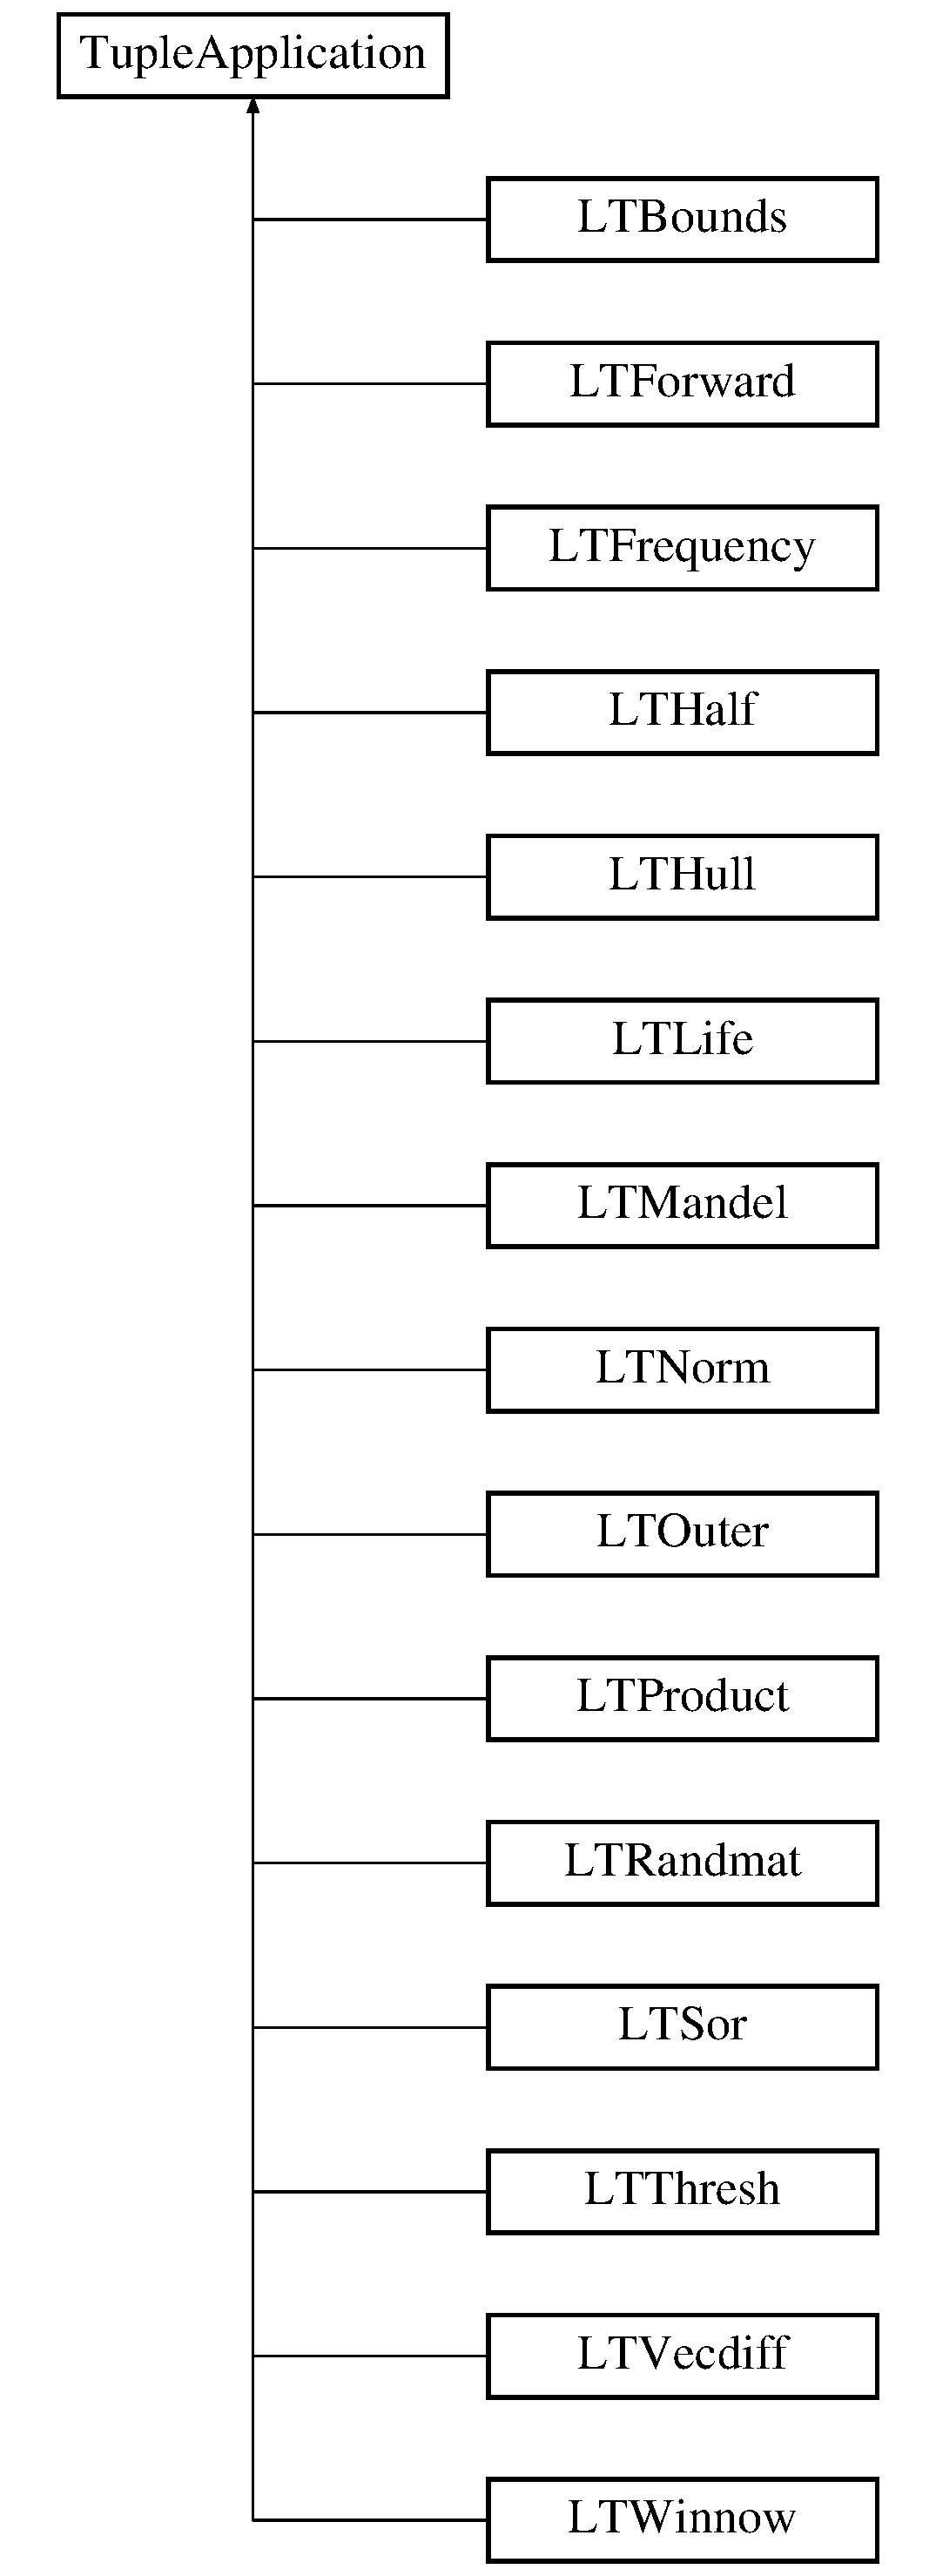
\includegraphics[height=12cm]{class_tuple_application}
\end{center}
\end{figure}
\subsection*{Public Member Functions}
\begin{CompactItemize}
\item 
void \hyperlink{class_tuple_application_892dbd783a1983228ac3865fb082f47a}{addInput} (int name, void $\ast$data)
\item 
void \hyperlink{class_tuple_application_985c26b37c8040ea51968af9caca9d3b}{addOutput} (int name, void $\ast$data)
\item 
int \hyperlink{class_tuple_application_9d0c51c481ef477787ffc2fd00116f4e}{start} (const char $\ast$host, int portNumber, int numWorkers)
\end{CompactItemize}
\subsection*{Protected Member Functions}
\begin{CompactItemize}
\item 
virtual void \hyperlink{class_tuple_application_e163c5a536de01c8b94b49528a17dab2}{consumeInput} ()=0
\item 
virtual void \hyperlink{class_tuple_application_ef6ae8bb1d697e4ed038b43320183c89}{work} ()=0
\item 
virtual void \hyperlink{class_tuple_application_8743dfcf17dedd52887c0b2ab170d8dc}{produceOutput} ()=0
\end{CompactItemize}
\subsection*{Protected Attributes}
\begin{CompactItemize}
\item 
std::map$<$ int, void $\ast$ $>$ \hyperlink{class_tuple_application_92a57e83bfd67542ae58e6a78720a3ef}{inputs}
\item 
std::map$<$ int, void $\ast$ $>$ \hyperlink{class_tuple_application_8abaaa3ef053827d70b3948e6f855082}{outputs}
\item 
struct context \hyperlink{class_tuple_application_773a45a8a04a872fd9c42b9ec07c8ebd}{ctx}
\end{CompactItemize}


\subsection{Detailed Description}
The common tuple application class allows LinuxTuples applications to be easily created. The class takes care of process creation and destruction, and makes sure outputs get carried onto the main process. Additionally, virtual functions are provided for workers and input/output processes. Things that need to be done in the tuple space should consider inheriting from this class. The class which all tuple applications should inherit from. 

\subsection{Member Function Documentation}
\hypertarget{class_tuple_application_892dbd783a1983228ac3865fb082f47a}{
\index{TupleApplication@{TupleApplication}!addInput@{addInput}}
\index{addInput@{addInput}!TupleApplication@{TupleApplication}}
\subsubsection[{addInput}]{\setlength{\rightskip}{0pt plus 5cm}void TupleApplication::addInput (int {\em name}, \/  void $\ast$ {\em data})}}
\label{class_tuple_application_892dbd783a1983228ac3865fb082f47a}


Set up input pointers. \begin{Desc}
\item[Parameters:]
\begin{description}
\item[{\em name}]the \char`\"{}name\char`\"{} of the data \item[{\em data}]the pointer to passed to the tuple-space \end{description}
\end{Desc}
\hypertarget{class_tuple_application_985c26b37c8040ea51968af9caca9d3b}{
\index{TupleApplication@{TupleApplication}!addOutput@{addOutput}}
\index{addOutput@{addOutput}!TupleApplication@{TupleApplication}}
\subsubsection[{addOutput}]{\setlength{\rightskip}{0pt plus 5cm}void TupleApplication::addOutput (int {\em name}, \/  void $\ast$ {\em data})}}
\label{class_tuple_application_985c26b37c8040ea51968af9caca9d3b}


Set up output pointers. \begin{Desc}
\item[Parameters:]
\begin{description}
\item[{\em name}]the \char`\"{}name\char`\"{} of the data \item[{\em data}]the pointer to passed to the tuple-space \end{description}
\end{Desc}
\hypertarget{class_tuple_application_e163c5a536de01c8b94b49528a17dab2}{
\index{TupleApplication@{TupleApplication}!consumeInput@{consumeInput}}
\index{consumeInput@{consumeInput}!TupleApplication@{TupleApplication}}
\subsubsection[{consumeInput}]{\setlength{\rightskip}{0pt plus 5cm}virtual void TupleApplication::consumeInput ()\hspace{0.3cm}{\tt  \mbox{[}protected, pure virtual\mbox{]}}}}
\label{class_tuple_application_e163c5a536de01c8b94b49528a17dab2}


The consume input process is spawned once and should distribute tasks to the worker processes. 

Implemented in \hyperlink{class_l_t_forward_6f3bbdf720e1899b0df8a8f222727086}{LTForward}, \hyperlink{class_l_t_half_fc07035f40f22a3f827504b13e8f99c9}{LTHalf}, \hyperlink{class_l_t_hull_e726f7fe6b16d8aa393045d4233a8447}{LTHull}, \hyperlink{class_l_t_life_da0a691f9bf8bb055a4fe953dd6eb809}{LTLife}, \hyperlink{class_l_t_mandel_15fb4ee93967f8717db22056f666f723}{LTMandel}, \hyperlink{class_l_t_bounds_ac6861a60c9a42ec8fc71025b481c380}{LTBounds}, \hyperlink{class_l_t_norm_58c0b2b050ac4e0fd5927fff451ae9ff}{LTNorm}, \hyperlink{class_l_t_outer_3e0493a0d06fbc86fe614edbd752eb8a}{LTOuter}, \hyperlink{class_l_t_product_377454ff007fa15f0bd378013bf1e6e6}{LTProduct}, \hyperlink{class_l_t_randmat_73181e409565b18c77d880dbf4123b26}{LTRandmat}, \hyperlink{class_l_t_sor_4fc4f0f914fc08f57f2ef5ba346cef1d}{LTSor}, \hyperlink{class_l_t_frequency_4ac4fa1a348246caf0d34506fcd09a64}{LTFrequency}, \hyperlink{class_l_t_thresh_b802b240b17b2c71cb758e1fe7585d72}{LTThresh}, \hyperlink{class_l_t_vecdiff_9daf31de467c9694e59b55936780dce8}{LTVecdiff}, and \hyperlink{class_l_t_winnow_ec961ab4e19c71b475903972111c20e9}{LTWinnow}.\hypertarget{class_tuple_application_8743dfcf17dedd52887c0b2ab170d8dc}{
\index{TupleApplication@{TupleApplication}!produceOutput@{produceOutput}}
\index{produceOutput@{produceOutput}!TupleApplication@{TupleApplication}}
\subsubsection[{produceOutput}]{\setlength{\rightskip}{0pt plus 5cm}virtual void TupleApplication::produceOutput ()\hspace{0.3cm}{\tt  \mbox{[}protected, pure virtual\mbox{]}}}}
\label{class_tuple_application_8743dfcf17dedd52887c0b2ab170d8dc}


The output producer decides when the tuple application is finished; once this function returns, the tuple application is complete. 

Implemented in \hyperlink{class_l_t_forward_56c27cd419407319f95afa4e7d43409a}{LTForward}, \hyperlink{class_l_t_half_bf36d89af87f94ff2aaff36338717f37}{LTHalf}, \hyperlink{class_l_t_hull_14a3bf005173aa79d0c7259579229f12}{LTHull}, \hyperlink{class_l_t_life_a0ac21131813f89a94c6ba7515e63c11}{LTLife}, \hyperlink{class_l_t_mandel_31cacf747914e03e6a87bb9af7dff67e}{LTMandel}, \hyperlink{class_l_t_bounds_028a451c099ee3377dc64a5a8ae9954f}{LTBounds}, \hyperlink{class_l_t_norm_2e142e5c7fabd218436f2abe99f4535b}{LTNorm}, \hyperlink{class_l_t_outer_2a12a006761b2e1132b84209d29fddac}{LTOuter}, \hyperlink{class_l_t_product_d03b068863d7b2febcbb7b11ebb819ca}{LTProduct}, \hyperlink{class_l_t_randmat_3adc0a50f5840dcc1228f4449e2b5da3}{LTRandmat}, \hyperlink{class_l_t_sor_19e969a6ab342ee86d86721fbd37e7a6}{LTSor}, \hyperlink{class_l_t_frequency_e80cd869c8935cb7fe553c6ad27e861b}{LTFrequency}, \hyperlink{class_l_t_thresh_41ce024f24320a5bd65239e98ac85587}{LTThresh}, \hyperlink{class_l_t_vecdiff_69d3c6e3c51052522d474cc75d11a2f2}{LTVecdiff}, and \hyperlink{class_l_t_winnow_865de8a240ae781c8cc5567082edc2ea}{LTWinnow}.\hypertarget{class_tuple_application_9d0c51c481ef477787ffc2fd00116f4e}{
\index{TupleApplication@{TupleApplication}!start@{start}}
\index{start@{start}!TupleApplication@{TupleApplication}}
\subsubsection[{start}]{\setlength{\rightskip}{0pt plus 5cm}int TupleApplication::start (const char $\ast$ {\em host}, \/  int {\em portNumber}, \/  int {\em numWorkers})}}
\label{class_tuple_application_9d0c51c481ef477787ffc2fd00116f4e}


Starts the tuple-space job. \hypertarget{class_tuple_application_ef6ae8bb1d697e4ed038b43320183c89}{
\index{TupleApplication@{TupleApplication}!work@{work}}
\index{work@{work}!TupleApplication@{TupleApplication}}
\subsubsection[{work}]{\setlength{\rightskip}{0pt plus 5cm}virtual void TupleApplication::work ()\hspace{0.3cm}{\tt  \mbox{[}protected, pure virtual\mbox{]}}}}
\label{class_tuple_application_ef6ae8bb1d697e4ed038b43320183c89}


Worker processes are created and killed after the output process has finished. 

Implemented in \hyperlink{class_l_t_forward_d98aff7a063bf6e8542046c6f2c097fa}{LTForward}, \hyperlink{class_l_t_half_e60dd430fb782498837492c0331e0dea}{LTHalf}, \hyperlink{class_l_t_hull_829b19b354bbe61d7cd5250819bd7b63}{LTHull}, \hyperlink{class_l_t_life_c0600864c1742c2a12e15992c539c2da}{LTLife}, \hyperlink{class_l_t_mandel_5ea4d32e6d16f64148bddbb940d732da}{LTMandel}, \hyperlink{class_l_t_bounds_877b72b63e19fbb7114bae270fe20c53}{LTBounds}, \hyperlink{class_l_t_norm_f0905a2c85b2e2713e98b9b22714a022}{LTNorm}, \hyperlink{class_l_t_outer_e0b1322b40271bb94c272b6117c8d16c}{LTOuter}, \hyperlink{class_l_t_product_1ba17b14e59b82c917f404cc9642bb09}{LTProduct}, \hyperlink{class_l_t_randmat_fffb75c16f2aaaa2f1bdb8a52f79234c}{LTRandmat}, \hyperlink{class_l_t_sor_48363c30cbba1c5ca61ed86260db94af}{LTSor}, \hyperlink{class_l_t_frequency_7c47cf36b228505f79225a3fe8a00f01}{LTFrequency}, \hyperlink{class_l_t_thresh_3cff6d04c7389a32e1dca924c7f93e23}{LTThresh}, \hyperlink{class_l_t_vecdiff_0117017e12284b1eb57532ca447684f6}{LTVecdiff}, and \hyperlink{class_l_t_winnow_472d0a232050f4674339029b1aa47531}{LTWinnow}.

\subsection{Member Data Documentation}
\hypertarget{class_tuple_application_773a45a8a04a872fd9c42b9ec07c8ebd}{
\index{TupleApplication@{TupleApplication}!ctx@{ctx}}
\index{ctx@{ctx}!TupleApplication@{TupleApplication}}
\subsubsection[{ctx}]{\setlength{\rightskip}{0pt plus 5cm}struct context {\bf TupleApplication::ctx}\hspace{0.3cm}{\tt  \mbox{[}read, protected\mbox{]}}}}
\label{class_tuple_application_773a45a8a04a872fd9c42b9ec07c8ebd}


Tuple-space context (LinuxTuples-specific). \hypertarget{class_tuple_application_92a57e83bfd67542ae58e6a78720a3ef}{
\index{TupleApplication@{TupleApplication}!inputs@{inputs}}
\index{inputs@{inputs}!TupleApplication@{TupleApplication}}
\subsubsection[{inputs}]{\setlength{\rightskip}{0pt plus 5cm}std::map$<$int, void$\ast$$>$ {\bf TupleApplication::inputs}\hspace{0.3cm}{\tt  \mbox{[}protected\mbox{]}}}}
\label{class_tuple_application_92a57e83bfd67542ae58e6a78720a3ef}


Inputs that should be available to all processes. \hypertarget{class_tuple_application_8abaaa3ef053827d70b3948e6f855082}{
\index{TupleApplication@{TupleApplication}!outputs@{outputs}}
\index{outputs@{outputs}!TupleApplication@{TupleApplication}}
\subsubsection[{outputs}]{\setlength{\rightskip}{0pt plus 5cm}std::map$<$int, void$\ast$$>$ {\bf TupleApplication::outputs}\hspace{0.3cm}{\tt  \mbox{[}protected\mbox{]}}}}
\label{class_tuple_application_8abaaa3ef053827d70b3948e6f855082}


Outputs that should be available to all processes, and that should be writable by the outputProducer process. 

The documentation for this class was generated from the following files:\begin{CompactItemize}
\item 
cowichan\_\-lt/src/\hyperlink{tuple__common_8hpp}{tuple\_\-common.hpp}\item 
cowichan\_\-lt/src/\hyperlink{tuple__common_8cpp}{tuple\_\-common.cpp}\end{CompactItemize}

\hypertarget{class_weighted_point}{
\section{WeightedPoint Class Reference}
\label{class_weighted_point}\index{WeightedPoint@{WeightedPoint}}
}
Two-dimensional point with an integer weight.  


{\tt \#include $<$cowichan.hpp$>$}

\subsection*{Public Member Functions}
\begin{CompactItemize}
\item 
\hyperlink{class_weighted_point_1fc45412653300484ff917c0df7716c7}{WeightedPoint} (\hyperlink{class_point}{Point} \hyperlink{class_weighted_point_ab8d1b3ff0e79d5b479e5f61eee1be23}{point}, \hyperlink{cowichan_8hpp_c96945095fd0ce7186a1d00a89f77d2c}{INT\_\-TYPE} \hyperlink{class_weighted_point_e41e421882ec4d21e70379120c2eab61}{weight})
\item 
\hyperlink{class_weighted_point_2a40faca74cd70475c325148056be842}{WeightedPoint} ()
\item 
\hyperlink{class_weighted_point_7e3ace28b58144f273b7d178b6fb0a06}{WeightedPoint} (\hyperlink{cowichan_8hpp_4d521b2c54a1f6312cc8fa04827eaf98}{real} x, \hyperlink{cowichan_8hpp_4d521b2c54a1f6312cc8fa04827eaf98}{real} y, \hyperlink{cowichan_8hpp_c96945095fd0ce7186a1d00a89f77d2c}{INT\_\-TYPE} \hyperlink{class_weighted_point_e41e421882ec4d21e70379120c2eab61}{weight})
\item 
bool \hyperlink{class_weighted_point_714944b15d891557a47a69b4d425da58}{operator$<$} (const \hyperlink{class_weighted_point}{WeightedPoint} \&rhs) const 
\item 
bool \hyperlink{class_weighted_point_f88df27a98c5849233572da3b504564c}{operator$<$=} (const \hyperlink{class_weighted_point}{WeightedPoint} \&rhs) const 
\end{CompactItemize}
\subsection*{Public Attributes}
\begin{CompactItemize}
\item 
\hyperlink{class_point}{Point} \hyperlink{class_weighted_point_ab8d1b3ff0e79d5b479e5f61eee1be23}{point}
\item 
\hyperlink{cowichan_8hpp_c96945095fd0ce7186a1d00a89f77d2c}{INT\_\-TYPE} \hyperlink{class_weighted_point_e41e421882ec4d21e70379120c2eab61}{weight}
\end{CompactItemize}


\subsection{Detailed Description}
Two-dimensional point with an integer weight. 

\subsection{Constructor \& Destructor Documentation}
\hypertarget{class_weighted_point_1fc45412653300484ff917c0df7716c7}{
\index{WeightedPoint@{WeightedPoint}!WeightedPoint@{WeightedPoint}}
\index{WeightedPoint@{WeightedPoint}!WeightedPoint@{WeightedPoint}}
\subsubsection[{WeightedPoint}]{\setlength{\rightskip}{0pt plus 5cm}WeightedPoint::WeightedPoint ({\bf Point} {\em point}, \/  {\bf INT\_\-TYPE} {\em weight})\hspace{0.3cm}{\tt  \mbox{[}inline\mbox{]}}}}
\label{class_weighted_point_1fc45412653300484ff917c0df7716c7}


Construct a weighted point. \begin{Desc}
\item[Parameters:]
\begin{description}
\item[{\em point}]point to copy. \item[{\em weight}]weight. \end{description}
\end{Desc}
\hypertarget{class_weighted_point_2a40faca74cd70475c325148056be842}{
\index{WeightedPoint@{WeightedPoint}!WeightedPoint@{WeightedPoint}}
\index{WeightedPoint@{WeightedPoint}!WeightedPoint@{WeightedPoint}}
\subsubsection[{WeightedPoint}]{\setlength{\rightskip}{0pt plus 5cm}WeightedPoint::WeightedPoint ()\hspace{0.3cm}{\tt  \mbox{[}inline\mbox{]}}}}
\label{class_weighted_point_2a40faca74cd70475c325148056be842}


Default constructor. \hypertarget{class_weighted_point_7e3ace28b58144f273b7d178b6fb0a06}{
\index{WeightedPoint@{WeightedPoint}!WeightedPoint@{WeightedPoint}}
\index{WeightedPoint@{WeightedPoint}!WeightedPoint@{WeightedPoint}}
\subsubsection[{WeightedPoint}]{\setlength{\rightskip}{0pt plus 5cm}WeightedPoint::WeightedPoint ({\bf real} {\em x}, \/  {\bf real} {\em y}, \/  {\bf INT\_\-TYPE} {\em weight})\hspace{0.3cm}{\tt  \mbox{[}inline\mbox{]}}}}
\label{class_weighted_point_7e3ace28b58144f273b7d178b6fb0a06}


Construct a weighted point. \begin{Desc}
\item[Parameters:]
\begin{description}
\item[{\em x}]x-coordinate. \item[{\em y}]y-coordinate. \item[{\em weight}]weight. \end{description}
\end{Desc}


\subsection{Member Function Documentation}
\hypertarget{class_weighted_point_714944b15d891557a47a69b4d425da58}{
\index{WeightedPoint@{WeightedPoint}!operator$<$@{operator$<$}}
\index{operator$<$@{operator$<$}!WeightedPoint@{WeightedPoint}}
\subsubsection[{operator$<$}]{\setlength{\rightskip}{0pt plus 5cm}bool WeightedPoint::operator$<$ (const {\bf WeightedPoint} \& {\em rhs}) const\hspace{0.3cm}{\tt  \mbox{[}inline\mbox{]}}}}
\label{class_weighted_point_714944b15d891557a47a69b4d425da58}


Less than comparison by weight. \begin{Desc}
\item[Parameters:]
\begin{description}
\item[{\em rhs}]right hand side weighted point. \end{description}
\end{Desc}
\begin{Desc}
\item[Returns:]Whether lhs $<$ rhs. \end{Desc}
\hypertarget{class_weighted_point_f88df27a98c5849233572da3b504564c}{
\index{WeightedPoint@{WeightedPoint}!operator$<$=@{operator$<$=}}
\index{operator$<$=@{operator$<$=}!WeightedPoint@{WeightedPoint}}
\subsubsection[{operator$<$=}]{\setlength{\rightskip}{0pt plus 5cm}bool WeightedPoint::operator$<$= (const {\bf WeightedPoint} \& {\em rhs}) const\hspace{0.3cm}{\tt  \mbox{[}inline\mbox{]}}}}
\label{class_weighted_point_f88df27a98c5849233572da3b504564c}


Less than or equal comparison by weight. \begin{Desc}
\item[Parameters:]
\begin{description}
\item[{\em rhs}]right hand side weighted point. \end{description}
\end{Desc}
\begin{Desc}
\item[Returns:]Whether lhs $<$= rhs. \end{Desc}


\subsection{Member Data Documentation}
\hypertarget{class_weighted_point_ab8d1b3ff0e79d5b479e5f61eee1be23}{
\index{WeightedPoint@{WeightedPoint}!point@{point}}
\index{point@{point}!WeightedPoint@{WeightedPoint}}
\subsubsection[{point}]{\setlength{\rightskip}{0pt plus 5cm}{\bf Point} {\bf WeightedPoint::point}}}
\label{class_weighted_point_ab8d1b3ff0e79d5b479e5f61eee1be23}


Two-dimensional point. \hypertarget{class_weighted_point_e41e421882ec4d21e70379120c2eab61}{
\index{WeightedPoint@{WeightedPoint}!weight@{weight}}
\index{weight@{weight}!WeightedPoint@{WeightedPoint}}
\subsubsection[{weight}]{\setlength{\rightskip}{0pt plus 5cm}{\bf INT\_\-TYPE} {\bf WeightedPoint::weight}}}
\label{class_weighted_point_e41e421882ec4d21e70379120c2eab61}


Weight. 

The documentation for this class was generated from the following file:\begin{CompactItemize}
\item 
cowichan/\hyperlink{cowichan_8hpp}{cowichan.hpp}\end{CompactItemize}

\chapter{File Documentation}
\hypertarget{cowichan_8cpp}{
\section{cowichan/cowichan.cpp File Reference}
\label{cowichan_8cpp}\index{cowichan/cowichan.cpp@{cowichan/cowichan.cpp}}
}
Implementation for \hyperlink{class_cowichan}{Cowichan} class and common routines for \hyperlink{class_cowichan}{Cowichan} programs.  


{\tt \#include \char`\"{}cowichan.hpp\char`\"{}}\par
\subsection*{Functions}
\begin{CompactItemize}
\item 
\hyperlink{cowichan_8hpp_4d521b2c54a1f6312cc8fa04827eaf98}{real} \hyperlink{cowichan_8cpp_eb2386a0fab0a548605cd5f0898da5b4}{uniform} (\hyperlink{cowichan_8hpp_4d521b2c54a1f6312cc8fa04827eaf98}{real} mean, \hyperlink{cowichan_8hpp_4d521b2c54a1f6312cc8fa04827eaf98}{real} range)
\item 
void \hyperlink{cowichan_8cpp_faa5a0a08b60255e5a59cbd3b1f5e45f}{out\_\-of\_\-memory} ()
\item 
void \hyperlink{cowichan_8cpp_501801b9dcd90a910432c7712ff763e7}{not\_\-enough\_\-points} ()
\item 
void \hyperlink{cowichan_8cpp_19e1551f7e954a984729d96c2c0bf5ba}{no\_\-cells\_\-alive} ()
\item 
INT64 \hyperlink{cowichan_8cpp_fa824504b2ae4f2f1ebbf5e6f76fb4fa}{get\_\-ticks} ()
\item 
INT64 \hyperlink{cowichan_8cpp_40356e6c8804a8f94e41c156ad368c83}{get\_\-freq} ()
\item 
void \hyperlink{cowichan_8cpp_560007e135455d06968b8a834d970cf9}{print\_\-elapsed\_\-time} (INT64 start, INT64 end)
\item 
void \hyperlink{cowichan_8cpp_1bf3d816eb607b5a06a97e05e9b95099}{timeInfo} (INT64 $\ast$start, INT64 $\ast$end, std::string message)
\end{CompactItemize}


\subsection{Detailed Description}
Implementation for \hyperlink{class_cowichan}{Cowichan} class and common routines for \hyperlink{class_cowichan}{Cowichan} programs. 



\subsection{Function Documentation}
\hypertarget{cowichan_8cpp_40356e6c8804a8f94e41c156ad368c83}{
\index{cowichan.cpp@{cowichan.cpp}!get\_\-freq@{get\_\-freq}}
\index{get\_\-freq@{get\_\-freq}!cowichan.cpp@{cowichan.cpp}}
\subsubsection[{get\_\-freq}]{\setlength{\rightskip}{0pt plus 5cm}INT64 get\_\-freq ()}}
\label{cowichan_8cpp_40356e6c8804a8f94e41c156ad368c83}


Get tick frequency. \begin{Desc}
\item[Returns:]Tick frequency. \end{Desc}
\hypertarget{cowichan_8cpp_fa824504b2ae4f2f1ebbf5e6f76fb4fa}{
\index{cowichan.cpp@{cowichan.cpp}!get\_\-ticks@{get\_\-ticks}}
\index{get\_\-ticks@{get\_\-ticks}!cowichan.cpp@{cowichan.cpp}}
\subsubsection[{get\_\-ticks}]{\setlength{\rightskip}{0pt plus 5cm}INT64 get\_\-ticks ()}}
\label{cowichan_8cpp_fa824504b2ae4f2f1ebbf5e6f76fb4fa}


Get tick count. \begin{Desc}
\item[Returns:]Tick count. \end{Desc}
\hypertarget{cowichan_8cpp_19e1551f7e954a984729d96c2c0bf5ba}{
\index{cowichan.cpp@{cowichan.cpp}!no\_\-cells\_\-alive@{no\_\-cells\_\-alive}}
\index{no\_\-cells\_\-alive@{no\_\-cells\_\-alive}!cowichan.cpp@{cowichan.cpp}}
\subsubsection[{no\_\-cells\_\-alive}]{\setlength{\rightskip}{0pt plus 5cm}void no\_\-cells\_\-alive ()}}
\label{cowichan_8cpp_19e1551f7e954a984729d96c2c0bf5ba}


Prints no cells alive message and exits. \hypertarget{cowichan_8cpp_501801b9dcd90a910432c7712ff763e7}{
\index{cowichan.cpp@{cowichan.cpp}!not\_\-enough\_\-points@{not\_\-enough\_\-points}}
\index{not\_\-enough\_\-points@{not\_\-enough\_\-points}!cowichan.cpp@{cowichan.cpp}}
\subsubsection[{not\_\-enough\_\-points}]{\setlength{\rightskip}{0pt plus 5cm}void not\_\-enough\_\-points ()}}
\label{cowichan_8cpp_501801b9dcd90a910432c7712ff763e7}


Prints not enough points message and exits. \hypertarget{cowichan_8cpp_faa5a0a08b60255e5a59cbd3b1f5e45f}{
\index{cowichan.cpp@{cowichan.cpp}!out\_\-of\_\-memory@{out\_\-of\_\-memory}}
\index{out\_\-of\_\-memory@{out\_\-of\_\-memory}!cowichan.cpp@{cowichan.cpp}}
\subsubsection[{out\_\-of\_\-memory}]{\setlength{\rightskip}{0pt plus 5cm}void out\_\-of\_\-memory ()}}
\label{cowichan_8cpp_faa5a0a08b60255e5a59cbd3b1f5e45f}


Prints out of memory message and exits. \hypertarget{cowichan_8cpp_560007e135455d06968b8a834d970cf9}{
\index{cowichan.cpp@{cowichan.cpp}!print\_\-elapsed\_\-time@{print\_\-elapsed\_\-time}}
\index{print\_\-elapsed\_\-time@{print\_\-elapsed\_\-time}!cowichan.cpp@{cowichan.cpp}}
\subsubsection[{print\_\-elapsed\_\-time}]{\setlength{\rightskip}{0pt plus 5cm}void print\_\-elapsed\_\-time (INT64 {\em start}, \/  INT64 {\em end})}}
\label{cowichan_8cpp_560007e135455d06968b8a834d970cf9}


Print elapsed time to std::cout. \begin{Desc}
\item[Parameters:]
\begin{description}
\item[{\em start}]initial tick count. \item[{\em end}]final tick count. \end{description}
\end{Desc}
\hypertarget{cowichan_8cpp_1bf3d816eb607b5a06a97e05e9b95099}{
\index{cowichan.cpp@{cowichan.cpp}!timeInfo@{timeInfo}}
\index{timeInfo@{timeInfo}!cowichan.cpp@{cowichan.cpp}}
\subsubsection[{timeInfo}]{\setlength{\rightskip}{0pt plus 5cm}void timeInfo (INT64 $\ast$ {\em start}, \/  INT64 $\ast$ {\em end}, \/  std::string {\em message})}}
\label{cowichan_8cpp_1bf3d816eb607b5a06a97e05e9b95099}


Does a sort of swap-out, printing progress. \begin{Desc}
\item[Parameters:]
\begin{description}
\item[{\em start}]pointer to initial tick count. \item[{\em end}]pointeger to final tick count. \item[{\em message}]message to print before the elapsed time. \end{description}
\end{Desc}
\hypertarget{cowichan_8cpp_eb2386a0fab0a548605cd5f0898da5b4}{
\index{cowichan.cpp@{cowichan.cpp}!uniform@{uniform}}
\index{uniform@{uniform}!cowichan.cpp@{cowichan.cpp}}
\subsubsection[{uniform}]{\setlength{\rightskip}{0pt plus 5cm}{\bf real} uniform ({\bf real} {\em mean}, \/  {\bf real} {\em range})}}
\label{cowichan_8cpp_eb2386a0fab0a548605cd5f0898da5b4}


Returns a pseudorandom number $\sim$ U\mbox{[}mean - range, mean + range\mbox{]}. \begin{Desc}
\item[Parameters:]
\begin{description}
\item[{\em mean}]mean. \item[{\em range}]range. \end{description}
\end{Desc}
\begin{Desc}
\item[Returns:]The pseudorandom number. \end{Desc}

\hypertarget{cowichan_8hpp}{
\section{cowichan/cowichan.hpp File Reference}
\label{cowichan_8hpp}\index{cowichan/cowichan.hpp@{cowichan/cowichan.hpp}}
}
Datatypes and common routines for \hyperlink{class_cowichan}{Cowichan} programs.  


{\tt \#include \char`\"{}cowichan\_\-defaults.hpp\char`\"{}}\par
{\tt \#include $<$iostream$>$}\par
{\tt \#include $<$cstdlib$>$}\par
{\tt \#include $<$ctime$>$}\par
{\tt \#include $<$cmath$>$}\par
{\tt \#include $<$algorithm$>$}\par
{\tt \#include $<$iomanip$>$}\par
{\tt \#include $<$climits$>$}\par
{\tt \#include $<$limits$>$}\par
{\tt \#include $<$string$>$}\par
{\tt \#include $<$cstring$>$}\par
{\tt \#include $<$windows.h$>$}\par
\subsection*{Classes}
\begin{CompactItemize}
\item 
class \hyperlink{class_point}{Point}
\begin{CompactList}\small\item\em Two-dimensional point. \item\end{CompactList}\item 
class \hyperlink{class_weighted_point}{WeightedPoint}
\begin{CompactList}\small\item\em Two-dimensional point with an integer weight. \item\end{CompactList}\item 
class \hyperlink{class_cowichan}{Cowichan}
\begin{CompactList}\small\item\em Base class for all C++ implementations. \item\end{CompactList}\end{CompactItemize}
\subsection*{Defines}
\begin{CompactItemize}
\item 
\#define \hyperlink{cowichan_8hpp_9adcfa1dcb92dd0d8757264ae41d1710}{TEST\_\-TIME}
\item 
\#define \hyperlink{cowichan_8hpp_e0937999ad4f52ae055b86396280604a}{SORT\_\-TIME}
\item 
\#define \hyperlink{cowichan_8hpp_7db5e8ee7c27e6fb5c9caf9d674ea949}{REAL\_\-TYPE}~float
\item 
\#define \hyperlink{cowichan_8hpp_9f8bbf20bc9432260a35b2f3cdb009f8}{MAXIMUM\_\-INT}~numeric\_\-limits$<$\hyperlink{cowichan_8hpp_c96945095fd0ce7186a1d00a89f77d2c}{INT\_\-TYPE}$>$::max()
\item 
\#define \hyperlink{cowichan_8hpp_af258621cee3ac54ad546ab5297c2476}{MINIMUM\_\-INT}~numeric\_\-limits$<$\hyperlink{cowichan_8hpp_c96945095fd0ce7186a1d00a89f77d2c}{INT\_\-TYPE}$>$::min()
\item 
\#define \hyperlink{cowichan_8hpp_753345ec3932dd32057b98ab9386efa0}{MAXIMUM\_\-REAL}~numeric\_\-limits$<$\hyperlink{cowichan_8hpp_4d521b2c54a1f6312cc8fa04827eaf98}{real}$>$::min()
\item 
\#define \hyperlink{cowichan_8hpp_e618a02a4bb148a144f9b9f99aa0b581}{MINIMUM\_\-REAL}~numeric\_\-limits$<$\hyperlink{cowichan_8hpp_4d521b2c54a1f6312cc8fa04827eaf98}{real}$>$::min()
\item 
\#define \hyperlink{cowichan_8hpp_bb50b5f693a0b64cdf91bca21cb464de}{INFINITY\_\-REAL}~numeric\_\-limits$<$\hyperlink{cowichan_8hpp_4d521b2c54a1f6312cc8fa04827eaf98}{real}$>$::infinity()
\item 
\#define \hyperlink{cowichan_8hpp_e2f68e53d100109588bb54ccc1c3d85b}{MATRIX\_\-RECT}(mtrx, row, col)~(mtrx)\mbox{[}(row)$\ast$this $\rightarrow$ nc + col\mbox{]}
\item 
\#define \hyperlink{cowichan_8hpp_2747f4d7d371c6ebdcaeb134876a2cf3}{MATRIX\_\-RECT\_\-NC}(mtrx, row, col, nc)~(mtrx)\mbox{[}(row)$\ast$(nc) + col\mbox{]}
\item 
\#define \hyperlink{cowichan_8hpp_79012ec47cbea66cd6664a54ca8a754c}{MATRIX\_\-SQUARE}(mtrx, row, col)~(mtrx)\mbox{[}(row)$\ast$this $\rightarrow$ n + col\mbox{]}
\item 
\#define \hyperlink{cowichan_8hpp_6772060ae1a2d5750934131acf95322a}{MATRIX\_\-SQUARE\_\-N}(mtrx, row, col, n)~(mtrx)\mbox{[}(row)$\ast$(n) + col\mbox{]}
\item 
\#define \hyperlink{cowichan_8hpp_f1d98fb728b5c7300f80dd782702d1dd}{MATRIX}~MATRIX\_\-SQUARE
\item 
\#define \hyperlink{cowichan_8hpp_41a3c329b378fa03397ed8a8925cbc73}{VECTOR}(vect, row)~(vect)\mbox{[}row\mbox{]}
\item 
\#define \hyperlink{cowichan_8hpp_bacaf90ccfec9927a6d97aa37f39917d}{DIAG}(mtrx, v)~(mtrx)\mbox{[}(v)$\ast$this $\rightarrow$ n + v\mbox{]}
\item 
\#define \hyperlink{cowichan_8hpp_7b818ef6ccf7d45bd25b07a402ca500f}{DIAG\_\-SZ}(mtrx, v, n)~(mtrx)\mbox{[}(v)$\ast$(n) + v\mbox{]}
\item 
\#define \hyperlink{cowichan_8hpp_07e1668b7974a041604d27b62cbe76f5}{NEW\_\-MATRIX\_\-RECT}(\_\-\_\-type)~(new \_\-\_\-type\mbox{[}this $\rightarrow$ nr $\ast$ this $\rightarrow$ nc\mbox{]})
\item 
\#define \hyperlink{cowichan_8hpp_03c9abf69e2e60f4ed74eebad85b750f}{NEW\_\-MATRIX\_\-SQUARE}(\_\-\_\-type)~(new \_\-\_\-type\mbox{[}this $\rightarrow$ n $\ast$ this $\rightarrow$ n\mbox{]})
\item 
\#define \hyperlink{cowichan_8hpp_e37a7bc1a3de6387853e097f2a8b24b5}{NEW\_\-VECTOR\_\-SZ}(\_\-\_\-type, \_\-\_\-num)~(new \_\-\_\-type\mbox{[}\_\-\_\-num\mbox{]})
\item 
\#define \hyperlink{cowichan_8hpp_71e0e9927a2730d38d0335484f7554fe}{NEW\_\-VECTOR}(\_\-\_\-type)~NEW\_\-VECTOR\_\-SZ(\_\-\_\-type, this $\rightarrow$ n)
\end{CompactItemize}
\subsection*{Typedefs}
\begin{CompactItemize}
\item 
typedef REAL\_\-TYPE \hyperlink{cowichan_8hpp_4d521b2c54a1f6312cc8fa04827eaf98}{real}
\item 
typedef UINT32 \hyperlink{cowichan_8hpp_c96945095fd0ce7186a1d00a89f77d2c}{INT\_\-TYPE}
\item 
typedef \hyperlink{cowichan_8hpp_c96945095fd0ce7186a1d00a89f77d2c}{INT\_\-TYPE} $\ast$ \hyperlink{cowichan_8hpp_82321152ddeeefe9c61350a42ed9e7af}{IntMatrix}
\item 
typedef bool $\ast$ \hyperlink{cowichan_8hpp_a64c8df2f1e9c8ea68a7bcc19aca683e}{BoolMatrix}
\item 
typedef \hyperlink{cowichan_8hpp_4d521b2c54a1f6312cc8fa04827eaf98}{real} $\ast$ \hyperlink{cowichan_8hpp_7b68f24757f8f24846e7b556a6563030}{RealMatrix}
\item 
typedef \hyperlink{cowichan_8hpp_c96945095fd0ce7186a1d00a89f77d2c}{INT\_\-TYPE} $\ast$ \hyperlink{cowichan_8hpp_9bab229b7d95f858be62c35cca6ff294}{IntVector}
\item 
typedef bool $\ast$ \hyperlink{cowichan_8hpp_69facfadf10e8e6e1b3ea0d02af7fef4}{BoolVector}
\item 
typedef \hyperlink{cowichan_8hpp_4d521b2c54a1f6312cc8fa04827eaf98}{real} $\ast$ \hyperlink{cowichan_8hpp_b40f3659328a6b06e3f83252e79e7b9a}{RealVector}
\item 
typedef \hyperlink{cowichan_8hpp_7b68f24757f8f24846e7b556a6563030}{RealMatrix} \hyperlink{cowichan_8hpp_3fb46f939e55c239fbc95656fc0f3399}{Matrix}
\item 
typedef \hyperlink{cowichan_8hpp_b40f3659328a6b06e3f83252e79e7b9a}{RealVector} \hyperlink{cowichan_8hpp_02bc1553e241b9b33408482658b3c355}{Vector}
\item 
typedef ptrdiff\_\-t \hyperlink{cowichan_8hpp_5b04577d5d21124855deaad298595371}{index\_\-t}
\item 
typedef \hyperlink{class_point}{Point} $\ast$ \hyperlink{cowichan_8hpp_1551f7def82edc60d7e37053954b7a07}{PointVector}
\item 
typedef \hyperlink{class_weighted_point}{WeightedPoint} $\ast$ \hyperlink{cowichan_8hpp_bd6eb1c54f195e0982817565e2ca9c31}{WeightedPointVector}
\end{CompactItemize}
\subsection*{Functions}
\begin{CompactItemize}
\item 
INT64 \hyperlink{cowichan_8hpp_fa824504b2ae4f2f1ebbf5e6f76fb4fa}{get\_\-ticks} ()
\item 
INT64 \hyperlink{cowichan_8hpp_40356e6c8804a8f94e41c156ad368c83}{get\_\-freq} ()
\item 
void \hyperlink{cowichan_8hpp_560007e135455d06968b8a834d970cf9}{print\_\-elapsed\_\-time} (INT64 start, INT64 end)
\item 
void \hyperlink{cowichan_8hpp_1bf3d816eb607b5a06a97e05e9b95099}{timeInfo} (INT64 $\ast$start, INT64 $\ast$end, std::string message)
\item 
void \hyperlink{cowichan_8hpp_faa5a0a08b60255e5a59cbd3b1f5e45f}{out\_\-of\_\-memory} ()
\item 
void \hyperlink{cowichan_8hpp_501801b9dcd90a910432c7712ff763e7}{not\_\-enough\_\-points} ()
\item 
void \hyperlink{cowichan_8hpp_19e1551f7e954a984729d96c2c0bf5ba}{no\_\-cells\_\-alive} ()
\item 
\hyperlink{cowichan_8hpp_4d521b2c54a1f6312cc8fa04827eaf98}{real} \hyperlink{cowichan_8hpp_eb2386a0fab0a548605cd5f0898da5b4}{uniform} (\hyperlink{cowichan_8hpp_4d521b2c54a1f6312cc8fa04827eaf98}{real} mean, \hyperlink{cowichan_8hpp_4d521b2c54a1f6312cc8fa04827eaf98}{real} range)
\end{CompactItemize}


\label{_details}
\hypertarget{_details}{}
\subsection{Detailed Description}
Datatypes and common routines for \hyperlink{class_cowichan}{Cowichan} programs. 



\subsection{Define Documentation}
\hypertarget{cowichan_8hpp_bacaf90ccfec9927a6d97aa37f39917d}{
\index{cowichan.hpp@{cowichan.hpp}!DIAG@{DIAG}}
\index{DIAG@{DIAG}!cowichan.hpp@{cowichan.hpp}}
\subsubsection[{DIAG}]{\setlength{\rightskip}{0pt plus 5cm}\#define DIAG(mtrx, \/  v)~(mtrx)\mbox{[}(v)$\ast$this $\rightarrow$ n + v\mbox{]}}}
\label{cowichan_8hpp_bacaf90ccfec9927a6d97aa37f39917d}


Access a square matrix diagonal element v from a class using member variable n as the matrix size. \hypertarget{cowichan_8hpp_7b818ef6ccf7d45bd25b07a402ca500f}{
\index{cowichan.hpp@{cowichan.hpp}!DIAG\_\-SZ@{DIAG\_\-SZ}}
\index{DIAG\_\-SZ@{DIAG\_\-SZ}!cowichan.hpp@{cowichan.hpp}}
\subsubsection[{DIAG\_\-SZ}]{\setlength{\rightskip}{0pt plus 5cm}\#define DIAG\_\-SZ(mtrx, \/  v, \/  n)~(mtrx)\mbox{[}(v)$\ast$(n) + v\mbox{]}}}
\label{cowichan_8hpp_7b818ef6ccf7d45bd25b07a402ca500f}


Access a square matrix diagonal element v using n as the matrix size. \hypertarget{cowichan_8hpp_bb50b5f693a0b64cdf91bca21cb464de}{
\index{cowichan.hpp@{cowichan.hpp}!INFINITY\_\-REAL@{INFINITY\_\-REAL}}
\index{INFINITY\_\-REAL@{INFINITY\_\-REAL}!cowichan.hpp@{cowichan.hpp}}
\subsubsection[{INFINITY\_\-REAL}]{\setlength{\rightskip}{0pt plus 5cm}\#define INFINITY\_\-REAL~numeric\_\-limits$<${\bf real}$>$::infinity()}}
\label{cowichan_8hpp_bb50b5f693a0b64cdf91bca21cb464de}


Real infinity value. \hypertarget{cowichan_8hpp_f1d98fb728b5c7300f80dd782702d1dd}{
\index{cowichan.hpp@{cowichan.hpp}!MATRIX@{MATRIX}}
\index{MATRIX@{MATRIX}!cowichan.hpp@{cowichan.hpp}}
\subsubsection[{MATRIX}]{\setlength{\rightskip}{0pt plus 5cm}\#define MATRIX~MATRIX\_\-SQUARE}}
\label{cowichan_8hpp_f1d98fb728b5c7300f80dd782702d1dd}


Same as MATRIX\_\-SQUARE (shorter name) \hypertarget{cowichan_8hpp_e2f68e53d100109588bb54ccc1c3d85b}{
\index{cowichan.hpp@{cowichan.hpp}!MATRIX\_\-RECT@{MATRIX\_\-RECT}}
\index{MATRIX\_\-RECT@{MATRIX\_\-RECT}!cowichan.hpp@{cowichan.hpp}}
\subsubsection[{MATRIX\_\-RECT}]{\setlength{\rightskip}{0pt plus 5cm}\#define MATRIX\_\-RECT(mtrx, \/  row, \/  col)~(mtrx)\mbox{[}(row)$\ast$this $\rightarrow$ nc + col\mbox{]}}}
\label{cowichan_8hpp_e2f68e53d100109588bb54ccc1c3d85b}


Access a rectangular matrix at row/col from a class using member variable nc as the number of columns. \hypertarget{cowichan_8hpp_2747f4d7d371c6ebdcaeb134876a2cf3}{
\index{cowichan.hpp@{cowichan.hpp}!MATRIX\_\-RECT\_\-NC@{MATRIX\_\-RECT\_\-NC}}
\index{MATRIX\_\-RECT\_\-NC@{MATRIX\_\-RECT\_\-NC}!cowichan.hpp@{cowichan.hpp}}
\subsubsection[{MATRIX\_\-RECT\_\-NC}]{\setlength{\rightskip}{0pt plus 5cm}\#define MATRIX\_\-RECT\_\-NC(mtrx, \/  row, \/  col, \/  nc)~(mtrx)\mbox{[}(row)$\ast$(nc) + col\mbox{]}}}
\label{cowichan_8hpp_2747f4d7d371c6ebdcaeb134876a2cf3}


Access a rectangular matrix at row/col using nc as the number of columns. \hypertarget{cowichan_8hpp_79012ec47cbea66cd6664a54ca8a754c}{
\index{cowichan.hpp@{cowichan.hpp}!MATRIX\_\-SQUARE@{MATRIX\_\-SQUARE}}
\index{MATRIX\_\-SQUARE@{MATRIX\_\-SQUARE}!cowichan.hpp@{cowichan.hpp}}
\subsubsection[{MATRIX\_\-SQUARE}]{\setlength{\rightskip}{0pt plus 5cm}\#define MATRIX\_\-SQUARE(mtrx, \/  row, \/  col)~(mtrx)\mbox{[}(row)$\ast$this $\rightarrow$ n + col\mbox{]}}}
\label{cowichan_8hpp_79012ec47cbea66cd6664a54ca8a754c}


Access a square matrix at row/col from a class using member variable n as the matrix size. \hypertarget{cowichan_8hpp_6772060ae1a2d5750934131acf95322a}{
\index{cowichan.hpp@{cowichan.hpp}!MATRIX\_\-SQUARE\_\-N@{MATRIX\_\-SQUARE\_\-N}}
\index{MATRIX\_\-SQUARE\_\-N@{MATRIX\_\-SQUARE\_\-N}!cowichan.hpp@{cowichan.hpp}}
\subsubsection[{MATRIX\_\-SQUARE\_\-N}]{\setlength{\rightskip}{0pt plus 5cm}\#define MATRIX\_\-SQUARE\_\-N(mtrx, \/  row, \/  col, \/  n)~(mtrx)\mbox{[}(row)$\ast$(n) + col\mbox{]}}}
\label{cowichan_8hpp_6772060ae1a2d5750934131acf95322a}


Access a square matrix at row/col using n as the matrix size. \hypertarget{cowichan_8hpp_9f8bbf20bc9432260a35b2f3cdb009f8}{
\index{cowichan.hpp@{cowichan.hpp}!MAXIMUM\_\-INT@{MAXIMUM\_\-INT}}
\index{MAXIMUM\_\-INT@{MAXIMUM\_\-INT}!cowichan.hpp@{cowichan.hpp}}
\subsubsection[{MAXIMUM\_\-INT}]{\setlength{\rightskip}{0pt plus 5cm}\#define MAXIMUM\_\-INT~numeric\_\-limits$<${\bf INT\_\-TYPE}$>$::max()}}
\label{cowichan_8hpp_9f8bbf20bc9432260a35b2f3cdb009f8}


Maximum integer value in matrices/vectors. \hypertarget{cowichan_8hpp_753345ec3932dd32057b98ab9386efa0}{
\index{cowichan.hpp@{cowichan.hpp}!MAXIMUM\_\-REAL@{MAXIMUM\_\-REAL}}
\index{MAXIMUM\_\-REAL@{MAXIMUM\_\-REAL}!cowichan.hpp@{cowichan.hpp}}
\subsubsection[{MAXIMUM\_\-REAL}]{\setlength{\rightskip}{0pt plus 5cm}\#define MAXIMUM\_\-REAL~numeric\_\-limits$<${\bf real}$>$::min()}}
\label{cowichan_8hpp_753345ec3932dd32057b98ab9386efa0}


Maximum real value in matrices/vectors. \hypertarget{cowichan_8hpp_af258621cee3ac54ad546ab5297c2476}{
\index{cowichan.hpp@{cowichan.hpp}!MINIMUM\_\-INT@{MINIMUM\_\-INT}}
\index{MINIMUM\_\-INT@{MINIMUM\_\-INT}!cowichan.hpp@{cowichan.hpp}}
\subsubsection[{MINIMUM\_\-INT}]{\setlength{\rightskip}{0pt plus 5cm}\#define MINIMUM\_\-INT~numeric\_\-limits$<${\bf INT\_\-TYPE}$>$::min()}}
\label{cowichan_8hpp_af258621cee3ac54ad546ab5297c2476}


Minimum integer value in matrices/vectors. \hypertarget{cowichan_8hpp_e618a02a4bb148a144f9b9f99aa0b581}{
\index{cowichan.hpp@{cowichan.hpp}!MINIMUM\_\-REAL@{MINIMUM\_\-REAL}}
\index{MINIMUM\_\-REAL@{MINIMUM\_\-REAL}!cowichan.hpp@{cowichan.hpp}}
\subsubsection[{MINIMUM\_\-REAL}]{\setlength{\rightskip}{0pt plus 5cm}\#define MINIMUM\_\-REAL~numeric\_\-limits$<${\bf real}$>$::min()}}
\label{cowichan_8hpp_e618a02a4bb148a144f9b9f99aa0b581}


Minimum real value in matrices/vectors. \hypertarget{cowichan_8hpp_07e1668b7974a041604d27b62cbe76f5}{
\index{cowichan.hpp@{cowichan.hpp}!NEW\_\-MATRIX\_\-RECT@{NEW\_\-MATRIX\_\-RECT}}
\index{NEW\_\-MATRIX\_\-RECT@{NEW\_\-MATRIX\_\-RECT}!cowichan.hpp@{cowichan.hpp}}
\subsubsection[{NEW\_\-MATRIX\_\-RECT}]{\setlength{\rightskip}{0pt plus 5cm}\#define NEW\_\-MATRIX\_\-RECT(\_\-\_\-type)~(new \_\-\_\-type\mbox{[}this $\rightarrow$ nr $\ast$ this $\rightarrow$ nc\mbox{]})}}
\label{cowichan_8hpp_07e1668b7974a041604d27b62cbe76f5}


Allocate a new rectangular matrix from a class using member variable nr as the number of rows and member variable nc as the number of columns. \hypertarget{cowichan_8hpp_03c9abf69e2e60f4ed74eebad85b750f}{
\index{cowichan.hpp@{cowichan.hpp}!NEW\_\-MATRIX\_\-SQUARE@{NEW\_\-MATRIX\_\-SQUARE}}
\index{NEW\_\-MATRIX\_\-SQUARE@{NEW\_\-MATRIX\_\-SQUARE}!cowichan.hpp@{cowichan.hpp}}
\subsubsection[{NEW\_\-MATRIX\_\-SQUARE}]{\setlength{\rightskip}{0pt plus 5cm}\#define NEW\_\-MATRIX\_\-SQUARE(\_\-\_\-type)~(new \_\-\_\-type\mbox{[}this $\rightarrow$ n $\ast$ this $\rightarrow$ n\mbox{]})}}
\label{cowichan_8hpp_03c9abf69e2e60f4ed74eebad85b750f}


Allocate a new square matrix from a class using member variable n as the matrix size. \hypertarget{cowichan_8hpp_71e0e9927a2730d38d0335484f7554fe}{
\index{cowichan.hpp@{cowichan.hpp}!NEW\_\-VECTOR@{NEW\_\-VECTOR}}
\index{NEW\_\-VECTOR@{NEW\_\-VECTOR}!cowichan.hpp@{cowichan.hpp}}
\subsubsection[{NEW\_\-VECTOR}]{\setlength{\rightskip}{0pt plus 5cm}\#define NEW\_\-VECTOR(\_\-\_\-type)~NEW\_\-VECTOR\_\-SZ(\_\-\_\-type, this $\rightarrow$ n)}}
\label{cowichan_8hpp_71e0e9927a2730d38d0335484f7554fe}


Allocate a new vector from a class using member variable n as the size of the vector. \hypertarget{cowichan_8hpp_e37a7bc1a3de6387853e097f2a8b24b5}{
\index{cowichan.hpp@{cowichan.hpp}!NEW\_\-VECTOR\_\-SZ@{NEW\_\-VECTOR\_\-SZ}}
\index{NEW\_\-VECTOR\_\-SZ@{NEW\_\-VECTOR\_\-SZ}!cowichan.hpp@{cowichan.hpp}}
\subsubsection[{NEW\_\-VECTOR\_\-SZ}]{\setlength{\rightskip}{0pt plus 5cm}\#define NEW\_\-VECTOR\_\-SZ(\_\-\_\-type, \/  \_\-\_\-num)~(new \_\-\_\-type\mbox{[}\_\-\_\-num\mbox{]})}}
\label{cowichan_8hpp_e37a7bc1a3de6387853e097f2a8b24b5}


Allocate a new vector of size \_\-\_\-num. \hypertarget{cowichan_8hpp_7db5e8ee7c27e6fb5c9caf9d674ea949}{
\index{cowichan.hpp@{cowichan.hpp}!REAL\_\-TYPE@{REAL\_\-TYPE}}
\index{REAL\_\-TYPE@{REAL\_\-TYPE}!cowichan.hpp@{cowichan.hpp}}
\subsubsection[{REAL\_\-TYPE}]{\setlength{\rightskip}{0pt plus 5cm}\#define REAL\_\-TYPE~float}}
\label{cowichan_8hpp_7db5e8ee7c27e6fb5c9caf9d674ea949}


Use IEEE single floating-point by default. \hypertarget{cowichan_8hpp_e0937999ad4f52ae055b86396280604a}{
\index{cowichan.hpp@{cowichan.hpp}!SORT\_\-TIME@{SORT\_\-TIME}}
\index{SORT\_\-TIME@{SORT\_\-TIME}!cowichan.hpp@{cowichan.hpp}}
\subsubsection[{SORT\_\-TIME}]{\setlength{\rightskip}{0pt plus 5cm}\#define SORT\_\-TIME}}
\label{cowichan_8hpp_e0937999ad4f52ae055b86396280604a}


Enables printing of sort time (in winnow). \hypertarget{cowichan_8hpp_9adcfa1dcb92dd0d8757264ae41d1710}{
\index{cowichan.hpp@{cowichan.hpp}!TEST\_\-TIME@{TEST\_\-TIME}}
\index{TEST\_\-TIME@{TEST\_\-TIME}!cowichan.hpp@{cowichan.hpp}}
\subsubsection[{TEST\_\-TIME}]{\setlength{\rightskip}{0pt plus 5cm}\#define TEST\_\-TIME}}
\label{cowichan_8hpp_9adcfa1dcb92dd0d8757264ae41d1710}


Enables printing of test time. \hypertarget{cowichan_8hpp_41a3c329b378fa03397ed8a8925cbc73}{
\index{cowichan.hpp@{cowichan.hpp}!VECTOR@{VECTOR}}
\index{VECTOR@{VECTOR}!cowichan.hpp@{cowichan.hpp}}
\subsubsection[{VECTOR}]{\setlength{\rightskip}{0pt plus 5cm}\#define VECTOR(vect, \/  row)~(vect)\mbox{[}row\mbox{]}}}
\label{cowichan_8hpp_41a3c329b378fa03397ed8a8925cbc73}


Access row of a vector. 

\subsection{Typedef Documentation}
\hypertarget{cowichan_8hpp_a64c8df2f1e9c8ea68a7bcc19aca683e}{
\index{cowichan.hpp@{cowichan.hpp}!BoolMatrix@{BoolMatrix}}
\index{BoolMatrix@{BoolMatrix}!cowichan.hpp@{cowichan.hpp}}
\subsubsection[{BoolMatrix}]{\setlength{\rightskip}{0pt plus 5cm}typedef bool$\ast$ {\bf BoolMatrix}}}
\label{cowichan_8hpp_a64c8df2f1e9c8ea68a7bcc19aca683e}


Boolean matrix type. \hypertarget{cowichan_8hpp_69facfadf10e8e6e1b3ea0d02af7fef4}{
\index{cowichan.hpp@{cowichan.hpp}!BoolVector@{BoolVector}}
\index{BoolVector@{BoolVector}!cowichan.hpp@{cowichan.hpp}}
\subsubsection[{BoolVector}]{\setlength{\rightskip}{0pt plus 5cm}typedef bool$\ast$ {\bf BoolVector}}}
\label{cowichan_8hpp_69facfadf10e8e6e1b3ea0d02af7fef4}


Boolean vector type. \hypertarget{cowichan_8hpp_5b04577d5d21124855deaad298595371}{
\index{cowichan.hpp@{cowichan.hpp}!index\_\-t@{index\_\-t}}
\index{index\_\-t@{index\_\-t}!cowichan.hpp@{cowichan.hpp}}
\subsubsection[{index\_\-t}]{\setlength{\rightskip}{0pt plus 5cm}typedef ptrdiff\_\-t {\bf index\_\-t}}}
\label{cowichan_8hpp_5b04577d5d21124855deaad298595371}


Index type (signed version of size\_\-t). \hypertarget{cowichan_8hpp_c96945095fd0ce7186a1d00a89f77d2c}{
\index{cowichan.hpp@{cowichan.hpp}!INT\_\-TYPE@{INT\_\-TYPE}}
\index{INT\_\-TYPE@{INT\_\-TYPE}!cowichan.hpp@{cowichan.hpp}}
\subsubsection[{INT\_\-TYPE}]{\setlength{\rightskip}{0pt plus 5cm}typedef UINT32 {\bf INT\_\-TYPE}}}
\label{cowichan_8hpp_c96945095fd0ce7186a1d00a89f77d2c}


Integer type (used in matrix/vector values). \hypertarget{cowichan_8hpp_82321152ddeeefe9c61350a42ed9e7af}{
\index{cowichan.hpp@{cowichan.hpp}!IntMatrix@{IntMatrix}}
\index{IntMatrix@{IntMatrix}!cowichan.hpp@{cowichan.hpp}}
\subsubsection[{IntMatrix}]{\setlength{\rightskip}{0pt plus 5cm}typedef {\bf INT\_\-TYPE}$\ast$ {\bf IntMatrix}}}
\label{cowichan_8hpp_82321152ddeeefe9c61350a42ed9e7af}


Integer matrix type. \hypertarget{cowichan_8hpp_9bab229b7d95f858be62c35cca6ff294}{
\index{cowichan.hpp@{cowichan.hpp}!IntVector@{IntVector}}
\index{IntVector@{IntVector}!cowichan.hpp@{cowichan.hpp}}
\subsubsection[{IntVector}]{\setlength{\rightskip}{0pt plus 5cm}typedef {\bf INT\_\-TYPE}$\ast$ {\bf IntVector}}}
\label{cowichan_8hpp_9bab229b7d95f858be62c35cca6ff294}


Integer vector type. \hypertarget{cowichan_8hpp_3fb46f939e55c239fbc95656fc0f3399}{
\index{cowichan.hpp@{cowichan.hpp}!Matrix@{Matrix}}
\index{Matrix@{Matrix}!cowichan.hpp@{cowichan.hpp}}
\subsubsection[{Matrix}]{\setlength{\rightskip}{0pt plus 5cm}typedef {\bf RealMatrix} {\bf Matrix}}}
\label{cowichan_8hpp_3fb46f939e55c239fbc95656fc0f3399}


Real matrix type (shorter name). \hypertarget{cowichan_8hpp_1551f7def82edc60d7e37053954b7a07}{
\index{cowichan.hpp@{cowichan.hpp}!PointVector@{PointVector}}
\index{PointVector@{PointVector}!cowichan.hpp@{cowichan.hpp}}
\subsubsection[{PointVector}]{\setlength{\rightskip}{0pt plus 5cm}typedef {\bf Point}$\ast$ {\bf PointVector}}}
\label{cowichan_8hpp_1551f7def82edc60d7e37053954b7a07}


Vector of points type. \hypertarget{cowichan_8hpp_4d521b2c54a1f6312cc8fa04827eaf98}{
\index{cowichan.hpp@{cowichan.hpp}!real@{real}}
\index{real@{real}!cowichan.hpp@{cowichan.hpp}}
\subsubsection[{real}]{\setlength{\rightskip}{0pt plus 5cm}typedef REAL\_\-TYPE {\bf real}}}
\label{cowichan_8hpp_4d521b2c54a1f6312cc8fa04827eaf98}


Real type (used in matrix/vector values). \hypertarget{cowichan_8hpp_7b68f24757f8f24846e7b556a6563030}{
\index{cowichan.hpp@{cowichan.hpp}!RealMatrix@{RealMatrix}}
\index{RealMatrix@{RealMatrix}!cowichan.hpp@{cowichan.hpp}}
\subsubsection[{RealMatrix}]{\setlength{\rightskip}{0pt plus 5cm}typedef {\bf real}$\ast$ {\bf RealMatrix}}}
\label{cowichan_8hpp_7b68f24757f8f24846e7b556a6563030}


Real matrix type. \hypertarget{cowichan_8hpp_b40f3659328a6b06e3f83252e79e7b9a}{
\index{cowichan.hpp@{cowichan.hpp}!RealVector@{RealVector}}
\index{RealVector@{RealVector}!cowichan.hpp@{cowichan.hpp}}
\subsubsection[{RealVector}]{\setlength{\rightskip}{0pt plus 5cm}typedef {\bf real}$\ast$ {\bf RealVector}}}
\label{cowichan_8hpp_b40f3659328a6b06e3f83252e79e7b9a}


Real vector type. \hypertarget{cowichan_8hpp_02bc1553e241b9b33408482658b3c355}{
\index{cowichan.hpp@{cowichan.hpp}!Vector@{Vector}}
\index{Vector@{Vector}!cowichan.hpp@{cowichan.hpp}}
\subsubsection[{Vector}]{\setlength{\rightskip}{0pt plus 5cm}typedef {\bf RealVector} {\bf Vector}}}
\label{cowichan_8hpp_02bc1553e241b9b33408482658b3c355}


Real vector type (shorter name). \hypertarget{cowichan_8hpp_bd6eb1c54f195e0982817565e2ca9c31}{
\index{cowichan.hpp@{cowichan.hpp}!WeightedPointVector@{WeightedPointVector}}
\index{WeightedPointVector@{WeightedPointVector}!cowichan.hpp@{cowichan.hpp}}
\subsubsection[{WeightedPointVector}]{\setlength{\rightskip}{0pt plus 5cm}typedef {\bf WeightedPoint}$\ast$ {\bf WeightedPointVector}}}
\label{cowichan_8hpp_bd6eb1c54f195e0982817565e2ca9c31}


Vector of weighted points type. 

\subsection{Function Documentation}
\hypertarget{cowichan_8hpp_40356e6c8804a8f94e41c156ad368c83}{
\index{cowichan.hpp@{cowichan.hpp}!get\_\-freq@{get\_\-freq}}
\index{get\_\-freq@{get\_\-freq}!cowichan.hpp@{cowichan.hpp}}
\subsubsection[{get\_\-freq}]{\setlength{\rightskip}{0pt plus 5cm}INT64 get\_\-freq ()}}
\label{cowichan_8hpp_40356e6c8804a8f94e41c156ad368c83}


Get tick frequency. \begin{Desc}
\item[Returns:]Tick frequency. \end{Desc}
\hypertarget{cowichan_8hpp_fa824504b2ae4f2f1ebbf5e6f76fb4fa}{
\index{cowichan.hpp@{cowichan.hpp}!get\_\-ticks@{get\_\-ticks}}
\index{get\_\-ticks@{get\_\-ticks}!cowichan.hpp@{cowichan.hpp}}
\subsubsection[{get\_\-ticks}]{\setlength{\rightskip}{0pt plus 5cm}INT64 get\_\-ticks ()}}
\label{cowichan_8hpp_fa824504b2ae4f2f1ebbf5e6f76fb4fa}


Get tick count. \begin{Desc}
\item[Returns:]Tick count. \end{Desc}
\hypertarget{cowichan_8hpp_19e1551f7e954a984729d96c2c0bf5ba}{
\index{cowichan.hpp@{cowichan.hpp}!no\_\-cells\_\-alive@{no\_\-cells\_\-alive}}
\index{no\_\-cells\_\-alive@{no\_\-cells\_\-alive}!cowichan.hpp@{cowichan.hpp}}
\subsubsection[{no\_\-cells\_\-alive}]{\setlength{\rightskip}{0pt plus 5cm}void no\_\-cells\_\-alive ()}}
\label{cowichan_8hpp_19e1551f7e954a984729d96c2c0bf5ba}


Prints no cells alive message and exits. \hypertarget{cowichan_8hpp_501801b9dcd90a910432c7712ff763e7}{
\index{cowichan.hpp@{cowichan.hpp}!not\_\-enough\_\-points@{not\_\-enough\_\-points}}
\index{not\_\-enough\_\-points@{not\_\-enough\_\-points}!cowichan.hpp@{cowichan.hpp}}
\subsubsection[{not\_\-enough\_\-points}]{\setlength{\rightskip}{0pt plus 5cm}void not\_\-enough\_\-points ()}}
\label{cowichan_8hpp_501801b9dcd90a910432c7712ff763e7}


Prints not enough points message and exits. \hypertarget{cowichan_8hpp_faa5a0a08b60255e5a59cbd3b1f5e45f}{
\index{cowichan.hpp@{cowichan.hpp}!out\_\-of\_\-memory@{out\_\-of\_\-memory}}
\index{out\_\-of\_\-memory@{out\_\-of\_\-memory}!cowichan.hpp@{cowichan.hpp}}
\subsubsection[{out\_\-of\_\-memory}]{\setlength{\rightskip}{0pt plus 5cm}void out\_\-of\_\-memory ()}}
\label{cowichan_8hpp_faa5a0a08b60255e5a59cbd3b1f5e45f}


Prints out of memory message and exits. \hypertarget{cowichan_8hpp_560007e135455d06968b8a834d970cf9}{
\index{cowichan.hpp@{cowichan.hpp}!print\_\-elapsed\_\-time@{print\_\-elapsed\_\-time}}
\index{print\_\-elapsed\_\-time@{print\_\-elapsed\_\-time}!cowichan.hpp@{cowichan.hpp}}
\subsubsection[{print\_\-elapsed\_\-time}]{\setlength{\rightskip}{0pt plus 5cm}void print\_\-elapsed\_\-time (INT64 {\em start}, \/  INT64 {\em end})}}
\label{cowichan_8hpp_560007e135455d06968b8a834d970cf9}


Print elapsed time to std::cout. \begin{Desc}
\item[Parameters:]
\begin{description}
\item[{\em start}]initial tick count. \item[{\em end}]final tick count. \end{description}
\end{Desc}
\hypertarget{cowichan_8hpp_1bf3d816eb607b5a06a97e05e9b95099}{
\index{cowichan.hpp@{cowichan.hpp}!timeInfo@{timeInfo}}
\index{timeInfo@{timeInfo}!cowichan.hpp@{cowichan.hpp}}
\subsubsection[{timeInfo}]{\setlength{\rightskip}{0pt plus 5cm}void timeInfo (INT64 $\ast$ {\em start}, \/  INT64 $\ast$ {\em end}, \/  std::string {\em message})}}
\label{cowichan_8hpp_1bf3d816eb607b5a06a97e05e9b95099}


Does a sort of swap-out, printing progress. \begin{Desc}
\item[Parameters:]
\begin{description}
\item[{\em start}]pointer to initial tick count. \item[{\em end}]pointeger to final tick count. \item[{\em message}]message to print before the elapsed time. \end{description}
\end{Desc}
\hypertarget{cowichan_8hpp_eb2386a0fab0a548605cd5f0898da5b4}{
\index{cowichan.hpp@{cowichan.hpp}!uniform@{uniform}}
\index{uniform@{uniform}!cowichan.hpp@{cowichan.hpp}}
\subsubsection[{uniform}]{\setlength{\rightskip}{0pt plus 5cm}{\bf real} uniform ({\bf real} {\em mean}, \/  {\bf real} {\em range})}}
\label{cowichan_8hpp_eb2386a0fab0a548605cd5f0898da5b4}


Returns a pseudorandom number $\sim$ U\mbox{[}mean - range, mean + range\mbox{]}. \begin{Desc}
\item[Parameters:]
\begin{description}
\item[{\em mean}]mean. \item[{\em range}]range. \end{description}
\end{Desc}
\begin{Desc}
\item[Returns:]The pseudorandom number. \end{Desc}

\hypertarget{cowichan__defaults_8hpp}{
\section{cowichan/cowichan\_\-defaults.hpp File Reference}
\label{cowichan__defaults_8hpp}\index{cowichan/cowichan\_\-defaults.hpp@{cowichan/cowichan\_\-defaults.hpp}}
}
Defaults for \hyperlink{class_cowichan}{Cowichan} programs.  


\subsection*{Defines}
\begin{CompactItemize}
\item 
\#define \hyperlink{cowichan__defaults_8hpp_30524c594b6941ca7822489d1794813b}{ALL\_\-NR}~15000
\item 
\#define \hyperlink{cowichan__defaults_8hpp_85076a3092aabd0bc4661e9184e2ddf3}{ALL\_\-NC}~15000
\item 
\#define \hyperlink{cowichan__defaults_8hpp_e36abbd26bf4ea979de0b63b1a37e349}{ALL\_\-N}~15000
\item 
\#define \hyperlink{cowichan__defaults_8hpp_0c6044d9326c14200929af66072b673a}{RAND\_\-MEAN}~0
\item 
\#define \hyperlink{cowichan__defaults_8hpp_40b63d443076ce61004bae3bf79a776b}{RAND\_\-RANGE}~20
\item 
\#define \hyperlink{cowichan__defaults_8hpp_32ee58f73d9de0d1d41ad46f7bff2719}{RAND\_\-SEED}~681304
\item 
\#define \hyperlink{cowichan__defaults_8hpp_d07476570307484eff173eedfbddd347}{RAND\_\-M}~56197
\item 
\#define \hyperlink{cowichan__defaults_8hpp_5f41a7e62c6e0138af5a65460416d6c7}{MANDEL\_\-NR}~ALL\_\-NR
\item 
\#define \hyperlink{cowichan__defaults_8hpp_d60d6cbcceef6bc7249b1480c829b7bb}{MANDEL\_\-NC}~ALL\_\-NC
\item 
\#define \hyperlink{cowichan__defaults_8hpp_5d8b0b1a78ed8a193734749178c248c1}{MANDEL\_\-X0}~0
\item 
\#define \hyperlink{cowichan__defaults_8hpp_47e550564bb994890b2ea6816155a0fe}{MANDEL\_\-Y0}~0
\item 
\#define \hyperlink{cowichan__defaults_8hpp_6fb2dcd18c6df1c377f613769d6314c3}{MANDEL\_\-DX}~1.5
\item 
\#define \hyperlink{cowichan__defaults_8hpp_b1759c852c10a8d03520a84beb5378fd}{MANDEL\_\-DY}~1.5
\item 
\#define \hyperlink{cowichan__defaults_8hpp_c911423783b8cba366d042acd8d062f3}{MANDEL\_\-INFINITY}~2.0
\item 
\#define \hyperlink{cowichan__defaults_8hpp_59c2aa73700269b6de563e60af48c6a3}{MANDEL\_\-MAX\_\-ITER}~150
\item 
\#define \hyperlink{cowichan__defaults_8hpp_6b2590531a8313fed76899a95ad3b625}{RANDMAT\_\-NR}~ALL\_\-NR
\item 
\#define \hyperlink{cowichan__defaults_8hpp_be3ee010372d99dfda2913d3d35a6a05}{RANDMAT\_\-NC}~ALL\_\-NC
\item 
\#define \hyperlink{cowichan__defaults_8hpp_7565d8f613d834da3b98134d4b564017}{RANDMAT\_\-A}~1291
\item 
\#define \hyperlink{cowichan__defaults_8hpp_cacc7f34c70c2ca998f0c1372ed1db83}{RANDMAT\_\-C}~917
\item 
\#define \hyperlink{cowichan__defaults_8hpp_3f8c101b36fa58d4d1d26cc4a77e1b51}{HALF\_\-NR}~ALL\_\-NR
\item 
\#define \hyperlink{cowichan__defaults_8hpp_d97fd174769938baa91d18ac273e1f93}{HALF\_\-NC}~ALL\_\-NC
\item 
\#define \hyperlink{cowichan__defaults_8hpp_966db6c2f5b3ed69daacad1d722b7071}{INVPERC\_\-NR}~ALL\_\-NR
\item 
\#define \hyperlink{cowichan__defaults_8hpp_3ae0f26f20ab30b6bbe513eff9a18291}{INVPERC\_\-NC}~ALL\_\-NC
\item 
\#define \hyperlink{cowichan__defaults_8hpp_cbaf3f96d8f75268024fb88255da23d9}{INVPERC\_\-NFILL}~1000000
\item 
\#define \hyperlink{cowichan__defaults_8hpp_4b80608f6c4617a66eba2f164afc4f3d}{THRESH\_\-NR}~ALL\_\-NR
\item 
\#define \hyperlink{cowichan__defaults_8hpp_7c356bfeab4913aa2e5dea26de44ebfc}{THRESH\_\-NC}~ALL\_\-NC
\item 
\#define \hyperlink{cowichan__defaults_8hpp_f85ccfff5fbed47416c64d4229d1234a}{THRESH\_\-PERCENT}~0.5
\item 
\#define \hyperlink{cowichan__defaults_8hpp_a597d047fbe34455bd7962e6e550adab}{LIFE\_\-NR}~ALL\_\-NR
\item 
\#define \hyperlink{cowichan__defaults_8hpp_9763036e0b951ebdb691f7336ecf0493}{LIFE\_\-NC}~ALL\_\-NC
\item 
\#define \hyperlink{cowichan__defaults_8hpp_02f3c90de37aa6314330a7e0cb68a1f5}{LIFE\_\-ITERATIONS}~10
\item 
\#define \hyperlink{cowichan__defaults_8hpp_cedd24970400253f48e19a285f8b8559}{WINNOW\_\-NR}~ALL\_\-NR
\item 
\#define \hyperlink{cowichan__defaults_8hpp_40f06800a12a97dde304a378d7d971cc}{WINNOW\_\-NC}~ALL\_\-NC
\item 
\#define \hyperlink{cowichan__defaults_8hpp_22c87347c9b1f8643a8b57e3d841303f}{WINNOW\_\-N}~ALL\_\-N
\item 
\#define \hyperlink{cowichan__defaults_8hpp_2ba93b0a30632568e28703c194c2345a}{NORM\_\-N}~ALL\_\-N
\item 
\#define \hyperlink{cowichan__defaults_8hpp_7f62220bbf93745fac5aa8e225f09126}{HULL\_\-N}~ALL\_\-N
\item 
\#define \hyperlink{cowichan__defaults_8hpp_113e7aa75d2b1403a5548913cd240cb4}{OUTER\_\-N}~ALL\_\-N
\item 
\#define \hyperlink{cowichan__defaults_8hpp_e1de0ce8df246861c84e405d66d37457}{GAUSS\_\-N}~ALL\_\-N
\item 
\#define \hyperlink{cowichan__defaults_8hpp_23487499c48e5b64d05fd2249be710c1}{SOR\_\-N}~ALL\_\-N
\item 
\#define \hyperlink{cowichan__defaults_8hpp_4b7aa2e2b41cee6b710c7ce48115f8ee}{SOR\_\-OMEGA}~0.9
\item 
\#define \hyperlink{cowichan__defaults_8hpp_e64dba51c415f6acbccbfd021a88769d}{SOR\_\-TOLERANCE}~10e-6
\item 
\#define \hyperlink{cowichan__defaults_8hpp_3673c55137aa755f4829b6b04329c379}{SOR\_\-MAX\_\-ITERS}~1000000
\item 
\#define \hyperlink{cowichan__defaults_8hpp_072a640a55e457c256faa59842e0368c}{PRODUCT\_\-N}~ALL\_\-N
\item 
\#define \hyperlink{cowichan__defaults_8hpp_d955f5a864096d87337347af906829b1}{VECDIFF\_\-N}~ALL\_\-N
\item 
\#define \hyperlink{cowichan__defaults_8hpp_5463dc5662d922fb1f8772a9e8e48672}{CHAIN\_\-NR}~ALL\_\-NR
\item 
\#define \hyperlink{cowichan__defaults_8hpp_fbc8b36ae001421db4f569c682ca7a45}{CHAIN\_\-NC}~ALL\_\-NC
\item 
\#define \hyperlink{cowichan__defaults_8hpp_40496e72e1bb9b2ca7ba854fa5679b8d}{CHAIN\_\-N}~ALL\_\-N
\end{CompactItemize}


\label{_details}
\hypertarget{_details}{}
\subsection{Detailed Description}
Defaults for \hyperlink{class_cowichan}{Cowichan} programs. 



\subsection{Define Documentation}
\hypertarget{cowichan__defaults_8hpp_e36abbd26bf4ea979de0b63b1a37e349}{
\index{cowichan\_\-defaults.hpp@{cowichan\_\-defaults.hpp}!ALL\_\-N@{ALL\_\-N}}
\index{ALL\_\-N@{ALL\_\-N}!cowichan_defaults.hpp@{cowichan\_\-defaults.hpp}}
\subsubsection[{ALL\_\-N}]{\setlength{\rightskip}{0pt plus 5cm}\#define ALL\_\-N~15000}}
\label{cowichan__defaults_8hpp_e36abbd26bf4ea979de0b63b1a37e349}


Default matrix size for square matrices for all problems. \hypertarget{cowichan__defaults_8hpp_85076a3092aabd0bc4661e9184e2ddf3}{
\index{cowichan\_\-defaults.hpp@{cowichan\_\-defaults.hpp}!ALL\_\-NC@{ALL\_\-NC}}
\index{ALL\_\-NC@{ALL\_\-NC}!cowichan_defaults.hpp@{cowichan\_\-defaults.hpp}}
\subsubsection[{ALL\_\-NC}]{\setlength{\rightskip}{0pt plus 5cm}\#define ALL\_\-NC~15000}}
\label{cowichan__defaults_8hpp_85076a3092aabd0bc4661e9184e2ddf3}


Default number of columns for rectangular matrices for all problems. \hypertarget{cowichan__defaults_8hpp_30524c594b6941ca7822489d1794813b}{
\index{cowichan\_\-defaults.hpp@{cowichan\_\-defaults.hpp}!ALL\_\-NR@{ALL\_\-NR}}
\index{ALL\_\-NR@{ALL\_\-NR}!cowichan_defaults.hpp@{cowichan\_\-defaults.hpp}}
\subsubsection[{ALL\_\-NR}]{\setlength{\rightskip}{0pt plus 5cm}\#define ALL\_\-NR~15000}}
\label{cowichan__defaults_8hpp_30524c594b6941ca7822489d1794813b}


Default number of rows for rectangular matrices for all problems. \hypertarget{cowichan__defaults_8hpp_40496e72e1bb9b2ca7ba854fa5679b8d}{
\index{cowichan\_\-defaults.hpp@{cowichan\_\-defaults.hpp}!CHAIN\_\-N@{CHAIN\_\-N}}
\index{CHAIN\_\-N@{CHAIN\_\-N}!cowichan_defaults.hpp@{cowichan\_\-defaults.hpp}}
\subsubsection[{CHAIN\_\-N}]{\setlength{\rightskip}{0pt plus 5cm}\#define CHAIN\_\-N~ALL\_\-N}}
\label{cowichan__defaults_8hpp_40496e72e1bb9b2ca7ba854fa5679b8d}


Default matrix size for square matrices for chain. \hypertarget{cowichan__defaults_8hpp_fbc8b36ae001421db4f569c682ca7a45}{
\index{cowichan\_\-defaults.hpp@{cowichan\_\-defaults.hpp}!CHAIN\_\-NC@{CHAIN\_\-NC}}
\index{CHAIN\_\-NC@{CHAIN\_\-NC}!cowichan_defaults.hpp@{cowichan\_\-defaults.hpp}}
\subsubsection[{CHAIN\_\-NC}]{\setlength{\rightskip}{0pt plus 5cm}\#define CHAIN\_\-NC~ALL\_\-NC}}
\label{cowichan__defaults_8hpp_fbc8b36ae001421db4f569c682ca7a45}


Default number of columns for rectangular matrices for chain. \hypertarget{cowichan__defaults_8hpp_5463dc5662d922fb1f8772a9e8e48672}{
\index{cowichan\_\-defaults.hpp@{cowichan\_\-defaults.hpp}!CHAIN\_\-NR@{CHAIN\_\-NR}}
\index{CHAIN\_\-NR@{CHAIN\_\-NR}!cowichan_defaults.hpp@{cowichan\_\-defaults.hpp}}
\subsubsection[{CHAIN\_\-NR}]{\setlength{\rightskip}{0pt plus 5cm}\#define CHAIN\_\-NR~ALL\_\-NR}}
\label{cowichan__defaults_8hpp_5463dc5662d922fb1f8772a9e8e48672}


Default number of rows for rectangular matrices for chain. \hypertarget{cowichan__defaults_8hpp_e1de0ce8df246861c84e405d66d37457}{
\index{cowichan\_\-defaults.hpp@{cowichan\_\-defaults.hpp}!GAUSS\_\-N@{GAUSS\_\-N}}
\index{GAUSS\_\-N@{GAUSS\_\-N}!cowichan_defaults.hpp@{cowichan\_\-defaults.hpp}}
\subsubsection[{GAUSS\_\-N}]{\setlength{\rightskip}{0pt plus 5cm}\#define GAUSS\_\-N~ALL\_\-N}}
\label{cowichan__defaults_8hpp_e1de0ce8df246861c84e405d66d37457}


Default square matrix size for gauss. \hypertarget{cowichan__defaults_8hpp_d97fd174769938baa91d18ac273e1f93}{
\index{cowichan\_\-defaults.hpp@{cowichan\_\-defaults.hpp}!HALF\_\-NC@{HALF\_\-NC}}
\index{HALF\_\-NC@{HALF\_\-NC}!cowichan_defaults.hpp@{cowichan\_\-defaults.hpp}}
\subsubsection[{HALF\_\-NC}]{\setlength{\rightskip}{0pt plus 5cm}\#define HALF\_\-NC~ALL\_\-NC}}
\label{cowichan__defaults_8hpp_d97fd174769938baa91d18ac273e1f93}


Default number of columns for half. \hypertarget{cowichan__defaults_8hpp_3f8c101b36fa58d4d1d26cc4a77e1b51}{
\index{cowichan\_\-defaults.hpp@{cowichan\_\-defaults.hpp}!HALF\_\-NR@{HALF\_\-NR}}
\index{HALF\_\-NR@{HALF\_\-NR}!cowichan_defaults.hpp@{cowichan\_\-defaults.hpp}}
\subsubsection[{HALF\_\-NR}]{\setlength{\rightskip}{0pt plus 5cm}\#define HALF\_\-NR~ALL\_\-NR}}
\label{cowichan__defaults_8hpp_3f8c101b36fa58d4d1d26cc4a77e1b51}


Default number of rows for half. \hypertarget{cowichan__defaults_8hpp_7f62220bbf93745fac5aa8e225f09126}{
\index{cowichan\_\-defaults.hpp@{cowichan\_\-defaults.hpp}!HULL\_\-N@{HULL\_\-N}}
\index{HULL\_\-N@{HULL\_\-N}!cowichan_defaults.hpp@{cowichan\_\-defaults.hpp}}
\subsubsection[{HULL\_\-N}]{\setlength{\rightskip}{0pt plus 5cm}\#define HULL\_\-N~ALL\_\-N}}
\label{cowichan__defaults_8hpp_7f62220bbf93745fac5aa8e225f09126}


Default square matrix size for hull. \hypertarget{cowichan__defaults_8hpp_3ae0f26f20ab30b6bbe513eff9a18291}{
\index{cowichan\_\-defaults.hpp@{cowichan\_\-defaults.hpp}!INVPERC\_\-NC@{INVPERC\_\-NC}}
\index{INVPERC\_\-NC@{INVPERC\_\-NC}!cowichan_defaults.hpp@{cowichan\_\-defaults.hpp}}
\subsubsection[{INVPERC\_\-NC}]{\setlength{\rightskip}{0pt plus 5cm}\#define INVPERC\_\-NC~ALL\_\-NC}}
\label{cowichan__defaults_8hpp_3ae0f26f20ab30b6bbe513eff9a18291}


Default number of columns for invperc. \hypertarget{cowichan__defaults_8hpp_cbaf3f96d8f75268024fb88255da23d9}{
\index{cowichan\_\-defaults.hpp@{cowichan\_\-defaults.hpp}!INVPERC\_\-NFILL@{INVPERC\_\-NFILL}}
\index{INVPERC\_\-NFILL@{INVPERC\_\-NFILL}!cowichan_defaults.hpp@{cowichan\_\-defaults.hpp}}
\subsubsection[{INVPERC\_\-NFILL}]{\setlength{\rightskip}{0pt plus 5cm}\#define INVPERC\_\-NFILL~1000000}}
\label{cowichan__defaults_8hpp_cbaf3f96d8f75268024fb88255da23d9}


Default number of cells to fill. \hypertarget{cowichan__defaults_8hpp_966db6c2f5b3ed69daacad1d722b7071}{
\index{cowichan\_\-defaults.hpp@{cowichan\_\-defaults.hpp}!INVPERC\_\-NR@{INVPERC\_\-NR}}
\index{INVPERC\_\-NR@{INVPERC\_\-NR}!cowichan_defaults.hpp@{cowichan\_\-defaults.hpp}}
\subsubsection[{INVPERC\_\-NR}]{\setlength{\rightskip}{0pt plus 5cm}\#define INVPERC\_\-NR~ALL\_\-NR}}
\label{cowichan__defaults_8hpp_966db6c2f5b3ed69daacad1d722b7071}


Default number of rows for invperc. \hypertarget{cowichan__defaults_8hpp_02f3c90de37aa6314330a7e0cb68a1f5}{
\index{cowichan\_\-defaults.hpp@{cowichan\_\-defaults.hpp}!LIFE\_\-ITERATIONS@{LIFE\_\-ITERATIONS}}
\index{LIFE\_\-ITERATIONS@{LIFE\_\-ITERATIONS}!cowichan_defaults.hpp@{cowichan\_\-defaults.hpp}}
\subsubsection[{LIFE\_\-ITERATIONS}]{\setlength{\rightskip}{0pt plus 5cm}\#define LIFE\_\-ITERATIONS~10}}
\label{cowichan__defaults_8hpp_02f3c90de37aa6314330a7e0cb68a1f5}


Default number of life iterations. \hypertarget{cowichan__defaults_8hpp_9763036e0b951ebdb691f7336ecf0493}{
\index{cowichan\_\-defaults.hpp@{cowichan\_\-defaults.hpp}!LIFE\_\-NC@{LIFE\_\-NC}}
\index{LIFE\_\-NC@{LIFE\_\-NC}!cowichan_defaults.hpp@{cowichan\_\-defaults.hpp}}
\subsubsection[{LIFE\_\-NC}]{\setlength{\rightskip}{0pt plus 5cm}\#define LIFE\_\-NC~ALL\_\-NC}}
\label{cowichan__defaults_8hpp_9763036e0b951ebdb691f7336ecf0493}


Default number of columns for life. \hypertarget{cowichan__defaults_8hpp_a597d047fbe34455bd7962e6e550adab}{
\index{cowichan\_\-defaults.hpp@{cowichan\_\-defaults.hpp}!LIFE\_\-NR@{LIFE\_\-NR}}
\index{LIFE\_\-NR@{LIFE\_\-NR}!cowichan_defaults.hpp@{cowichan\_\-defaults.hpp}}
\subsubsection[{LIFE\_\-NR}]{\setlength{\rightskip}{0pt plus 5cm}\#define LIFE\_\-NR~ALL\_\-NR}}
\label{cowichan__defaults_8hpp_a597d047fbe34455bd7962e6e550adab}


Default number of rows for life. \hypertarget{cowichan__defaults_8hpp_6fb2dcd18c6df1c377f613769d6314c3}{
\index{cowichan\_\-defaults.hpp@{cowichan\_\-defaults.hpp}!MANDEL\_\-DX@{MANDEL\_\-DX}}
\index{MANDEL\_\-DX@{MANDEL\_\-DX}!cowichan_defaults.hpp@{cowichan\_\-defaults.hpp}}
\subsubsection[{MANDEL\_\-DX}]{\setlength{\rightskip}{0pt plus 5cm}\#define MANDEL\_\-DX~1.5}}
\label{cowichan__defaults_8hpp_6fb2dcd18c6df1c377f613769d6314c3}


Default extent of the region along the x axis. \hypertarget{cowichan__defaults_8hpp_b1759c852c10a8d03520a84beb5378fd}{
\index{cowichan\_\-defaults.hpp@{cowichan\_\-defaults.hpp}!MANDEL\_\-DY@{MANDEL\_\-DY}}
\index{MANDEL\_\-DY@{MANDEL\_\-DY}!cowichan_defaults.hpp@{cowichan\_\-defaults.hpp}}
\subsubsection[{MANDEL\_\-DY}]{\setlength{\rightskip}{0pt plus 5cm}\#define MANDEL\_\-DY~1.5}}
\label{cowichan__defaults_8hpp_b1759c852c10a8d03520a84beb5378fd}


Default extent of the region along the y axis. \hypertarget{cowichan__defaults_8hpp_c911423783b8cba366d042acd8d062f3}{
\index{cowichan\_\-defaults.hpp@{cowichan\_\-defaults.hpp}!MANDEL\_\-INFINITY@{MANDEL\_\-INFINITY}}
\index{MANDEL\_\-INFINITY@{MANDEL\_\-INFINITY}!cowichan_defaults.hpp@{cowichan\_\-defaults.hpp}}
\subsubsection[{MANDEL\_\-INFINITY}]{\setlength{\rightskip}{0pt plus 5cm}\#define MANDEL\_\-INFINITY~2.0}}
\label{cowichan__defaults_8hpp_c911423783b8cba366d042acd8d062f3}


Default mandel infinity. \hypertarget{cowichan__defaults_8hpp_59c2aa73700269b6de563e60af48c6a3}{
\index{cowichan\_\-defaults.hpp@{cowichan\_\-defaults.hpp}!MANDEL\_\-MAX\_\-ITER@{MANDEL\_\-MAX\_\-ITER}}
\index{MANDEL\_\-MAX\_\-ITER@{MANDEL\_\-MAX\_\-ITER}!cowichan_defaults.hpp@{cowichan\_\-defaults.hpp}}
\subsubsection[{MANDEL\_\-MAX\_\-ITER}]{\setlength{\rightskip}{0pt plus 5cm}\#define MANDEL\_\-MAX\_\-ITER~150}}
\label{cowichan__defaults_8hpp_59c2aa73700269b6de563e60af48c6a3}


Default mandel maximum number of iterations. \hypertarget{cowichan__defaults_8hpp_d60d6cbcceef6bc7249b1480c829b7bb}{
\index{cowichan\_\-defaults.hpp@{cowichan\_\-defaults.hpp}!MANDEL\_\-NC@{MANDEL\_\-NC}}
\index{MANDEL\_\-NC@{MANDEL\_\-NC}!cowichan_defaults.hpp@{cowichan\_\-defaults.hpp}}
\subsubsection[{MANDEL\_\-NC}]{\setlength{\rightskip}{0pt plus 5cm}\#define MANDEL\_\-NC~ALL\_\-NC}}
\label{cowichan__defaults_8hpp_d60d6cbcceef6bc7249b1480c829b7bb}


Default number of columns for mandel. \hypertarget{cowichan__defaults_8hpp_5f41a7e62c6e0138af5a65460416d6c7}{
\index{cowichan\_\-defaults.hpp@{cowichan\_\-defaults.hpp}!MANDEL\_\-NR@{MANDEL\_\-NR}}
\index{MANDEL\_\-NR@{MANDEL\_\-NR}!cowichan_defaults.hpp@{cowichan\_\-defaults.hpp}}
\subsubsection[{MANDEL\_\-NR}]{\setlength{\rightskip}{0pt plus 5cm}\#define MANDEL\_\-NR~ALL\_\-NR}}
\label{cowichan__defaults_8hpp_5f41a7e62c6e0138af5a65460416d6c7}


Default number of rows for mandel. \hypertarget{cowichan__defaults_8hpp_5d8b0b1a78ed8a193734749178c248c1}{
\index{cowichan\_\-defaults.hpp@{cowichan\_\-defaults.hpp}!MANDEL\_\-X0@{MANDEL\_\-X0}}
\index{MANDEL\_\-X0@{MANDEL\_\-X0}!cowichan_defaults.hpp@{cowichan\_\-defaults.hpp}}
\subsubsection[{MANDEL\_\-X0}]{\setlength{\rightskip}{0pt plus 5cm}\#define MANDEL\_\-X0~0}}
\label{cowichan__defaults_8hpp_5d8b0b1a78ed8a193734749178c248c1}


Default x-coordinate of the lower left corner. \hypertarget{cowichan__defaults_8hpp_47e550564bb994890b2ea6816155a0fe}{
\index{cowichan\_\-defaults.hpp@{cowichan\_\-defaults.hpp}!MANDEL\_\-Y0@{MANDEL\_\-Y0}}
\index{MANDEL\_\-Y0@{MANDEL\_\-Y0}!cowichan_defaults.hpp@{cowichan\_\-defaults.hpp}}
\subsubsection[{MANDEL\_\-Y0}]{\setlength{\rightskip}{0pt plus 5cm}\#define MANDEL\_\-Y0~0}}
\label{cowichan__defaults_8hpp_47e550564bb994890b2ea6816155a0fe}


Default y-coordinate of the lower left corner \hypertarget{cowichan__defaults_8hpp_2ba93b0a30632568e28703c194c2345a}{
\index{cowichan\_\-defaults.hpp@{cowichan\_\-defaults.hpp}!NORM\_\-N@{NORM\_\-N}}
\index{NORM\_\-N@{NORM\_\-N}!cowichan_defaults.hpp@{cowichan\_\-defaults.hpp}}
\subsubsection[{NORM\_\-N}]{\setlength{\rightskip}{0pt plus 5cm}\#define NORM\_\-N~ALL\_\-N}}
\label{cowichan__defaults_8hpp_2ba93b0a30632568e28703c194c2345a}


Default square matrix size for norm. \hypertarget{cowichan__defaults_8hpp_113e7aa75d2b1403a5548913cd240cb4}{
\index{cowichan\_\-defaults.hpp@{cowichan\_\-defaults.hpp}!OUTER\_\-N@{OUTER\_\-N}}
\index{OUTER\_\-N@{OUTER\_\-N}!cowichan_defaults.hpp@{cowichan\_\-defaults.hpp}}
\subsubsection[{OUTER\_\-N}]{\setlength{\rightskip}{0pt plus 5cm}\#define OUTER\_\-N~ALL\_\-N}}
\label{cowichan__defaults_8hpp_113e7aa75d2b1403a5548913cd240cb4}


Default square matrix size for outer. \hypertarget{cowichan__defaults_8hpp_072a640a55e457c256faa59842e0368c}{
\index{cowichan\_\-defaults.hpp@{cowichan\_\-defaults.hpp}!PRODUCT\_\-N@{PRODUCT\_\-N}}
\index{PRODUCT\_\-N@{PRODUCT\_\-N}!cowichan_defaults.hpp@{cowichan\_\-defaults.hpp}}
\subsubsection[{PRODUCT\_\-N}]{\setlength{\rightskip}{0pt plus 5cm}\#define PRODUCT\_\-N~ALL\_\-N}}
\label{cowichan__defaults_8hpp_072a640a55e457c256faa59842e0368c}


Default square matrix size for product. \hypertarget{cowichan__defaults_8hpp_d07476570307484eff173eedfbddd347}{
\index{cowichan\_\-defaults.hpp@{cowichan\_\-defaults.hpp}!RAND\_\-M@{RAND\_\-M}}
\index{RAND\_\-M@{RAND\_\-M}!cowichan_defaults.hpp@{cowichan\_\-defaults.hpp}}
\subsubsection[{RAND\_\-M}]{\setlength{\rightskip}{0pt plus 5cm}\#define RAND\_\-M~56197}}
\label{cowichan__defaults_8hpp_d07476570307484eff173eedfbddd347}


Default random number limit. \hypertarget{cowichan__defaults_8hpp_0c6044d9326c14200929af66072b673a}{
\index{cowichan\_\-defaults.hpp@{cowichan\_\-defaults.hpp}!RAND\_\-MEAN@{RAND\_\-MEAN}}
\index{RAND\_\-MEAN@{RAND\_\-MEAN}!cowichan_defaults.hpp@{cowichan\_\-defaults.hpp}}
\subsubsection[{RAND\_\-MEAN}]{\setlength{\rightskip}{0pt plus 5cm}\#define RAND\_\-MEAN~0}}
\label{cowichan__defaults_8hpp_0c6044d9326c14200929af66072b673a}


Default random number mean for inputs. \hypertarget{cowichan__defaults_8hpp_40b63d443076ce61004bae3bf79a776b}{
\index{cowichan\_\-defaults.hpp@{cowichan\_\-defaults.hpp}!RAND\_\-RANGE@{RAND\_\-RANGE}}
\index{RAND\_\-RANGE@{RAND\_\-RANGE}!cowichan_defaults.hpp@{cowichan\_\-defaults.hpp}}
\subsubsection[{RAND\_\-RANGE}]{\setlength{\rightskip}{0pt plus 5cm}\#define RAND\_\-RANGE~20}}
\label{cowichan__defaults_8hpp_40b63d443076ce61004bae3bf79a776b}


Default random number range for inputs. \hypertarget{cowichan__defaults_8hpp_32ee58f73d9de0d1d41ad46f7bff2719}{
\index{cowichan\_\-defaults.hpp@{cowichan\_\-defaults.hpp}!RAND\_\-SEED@{RAND\_\-SEED}}
\index{RAND\_\-SEED@{RAND\_\-SEED}!cowichan_defaults.hpp@{cowichan\_\-defaults.hpp}}
\subsubsection[{RAND\_\-SEED}]{\setlength{\rightskip}{0pt plus 5cm}\#define RAND\_\-SEED~681304}}
\label{cowichan__defaults_8hpp_32ee58f73d9de0d1d41ad46f7bff2719}


Default random number seed. \hypertarget{cowichan__defaults_8hpp_7565d8f613d834da3b98134d4b564017}{
\index{cowichan\_\-defaults.hpp@{cowichan\_\-defaults.hpp}!RANDMAT\_\-A@{RANDMAT\_\-A}}
\index{RANDMAT\_\-A@{RANDMAT\_\-A}!cowichan_defaults.hpp@{cowichan\_\-defaults.hpp}}
\subsubsection[{RANDMAT\_\-A}]{\setlength{\rightskip}{0pt plus 5cm}\#define RANDMAT\_\-A~1291}}
\label{cowichan__defaults_8hpp_7565d8f613d834da3b98134d4b564017}


Default constant A for randmat. \hypertarget{cowichan__defaults_8hpp_cacc7f34c70c2ca998f0c1372ed1db83}{
\index{cowichan\_\-defaults.hpp@{cowichan\_\-defaults.hpp}!RANDMAT\_\-C@{RANDMAT\_\-C}}
\index{RANDMAT\_\-C@{RANDMAT\_\-C}!cowichan_defaults.hpp@{cowichan\_\-defaults.hpp}}
\subsubsection[{RANDMAT\_\-C}]{\setlength{\rightskip}{0pt plus 5cm}\#define RANDMAT\_\-C~917}}
\label{cowichan__defaults_8hpp_cacc7f34c70c2ca998f0c1372ed1db83}


Default constant C for randmat. \hypertarget{cowichan__defaults_8hpp_be3ee010372d99dfda2913d3d35a6a05}{
\index{cowichan\_\-defaults.hpp@{cowichan\_\-defaults.hpp}!RANDMAT\_\-NC@{RANDMAT\_\-NC}}
\index{RANDMAT\_\-NC@{RANDMAT\_\-NC}!cowichan_defaults.hpp@{cowichan\_\-defaults.hpp}}
\subsubsection[{RANDMAT\_\-NC}]{\setlength{\rightskip}{0pt plus 5cm}\#define RANDMAT\_\-NC~ALL\_\-NC}}
\label{cowichan__defaults_8hpp_be3ee010372d99dfda2913d3d35a6a05}


Default number of columns for randmat. \hypertarget{cowichan__defaults_8hpp_6b2590531a8313fed76899a95ad3b625}{
\index{cowichan\_\-defaults.hpp@{cowichan\_\-defaults.hpp}!RANDMAT\_\-NR@{RANDMAT\_\-NR}}
\index{RANDMAT\_\-NR@{RANDMAT\_\-NR}!cowichan_defaults.hpp@{cowichan\_\-defaults.hpp}}
\subsubsection[{RANDMAT\_\-NR}]{\setlength{\rightskip}{0pt plus 5cm}\#define RANDMAT\_\-NR~ALL\_\-NR}}
\label{cowichan__defaults_8hpp_6b2590531a8313fed76899a95ad3b625}


Default number of rows for randmat. \hypertarget{cowichan__defaults_8hpp_3673c55137aa755f4829b6b04329c379}{
\index{cowichan\_\-defaults.hpp@{cowichan\_\-defaults.hpp}!SOR\_\-MAX\_\-ITERS@{SOR\_\-MAX\_\-ITERS}}
\index{SOR\_\-MAX\_\-ITERS@{SOR\_\-MAX\_\-ITERS}!cowichan_defaults.hpp@{cowichan\_\-defaults.hpp}}
\subsubsection[{SOR\_\-MAX\_\-ITERS}]{\setlength{\rightskip}{0pt plus 5cm}\#define SOR\_\-MAX\_\-ITERS~1000000}}
\label{cowichan__defaults_8hpp_3673c55137aa755f4829b6b04329c379}


Default maximum number of iterations for sor. \hypertarget{cowichan__defaults_8hpp_23487499c48e5b64d05fd2249be710c1}{
\index{cowichan\_\-defaults.hpp@{cowichan\_\-defaults.hpp}!SOR\_\-N@{SOR\_\-N}}
\index{SOR\_\-N@{SOR\_\-N}!cowichan_defaults.hpp@{cowichan\_\-defaults.hpp}}
\subsubsection[{SOR\_\-N}]{\setlength{\rightskip}{0pt plus 5cm}\#define SOR\_\-N~ALL\_\-N}}
\label{cowichan__defaults_8hpp_23487499c48e5b64d05fd2249be710c1}


Default square matrix size for sor. \hypertarget{cowichan__defaults_8hpp_4b7aa2e2b41cee6b710c7ce48115f8ee}{
\index{cowichan\_\-defaults.hpp@{cowichan\_\-defaults.hpp}!SOR\_\-OMEGA@{SOR\_\-OMEGA}}
\index{SOR\_\-OMEGA@{SOR\_\-OMEGA}!cowichan_defaults.hpp@{cowichan\_\-defaults.hpp}}
\subsubsection[{SOR\_\-OMEGA}]{\setlength{\rightskip}{0pt plus 5cm}\#define SOR\_\-OMEGA~0.9}}
\label{cowichan__defaults_8hpp_4b7aa2e2b41cee6b710c7ce48115f8ee}


Default omega for sor. \hypertarget{cowichan__defaults_8hpp_e64dba51c415f6acbccbfd021a88769d}{
\index{cowichan\_\-defaults.hpp@{cowichan\_\-defaults.hpp}!SOR\_\-TOLERANCE@{SOR\_\-TOLERANCE}}
\index{SOR\_\-TOLERANCE@{SOR\_\-TOLERANCE}!cowichan_defaults.hpp@{cowichan\_\-defaults.hpp}}
\subsubsection[{SOR\_\-TOLERANCE}]{\setlength{\rightskip}{0pt plus 5cm}\#define SOR\_\-TOLERANCE~10e-6}}
\label{cowichan__defaults_8hpp_e64dba51c415f6acbccbfd021a88769d}


Default floating point tolerance for sor. \hypertarget{cowichan__defaults_8hpp_7c356bfeab4913aa2e5dea26de44ebfc}{
\index{cowichan\_\-defaults.hpp@{cowichan\_\-defaults.hpp}!THRESH\_\-NC@{THRESH\_\-NC}}
\index{THRESH\_\-NC@{THRESH\_\-NC}!cowichan_defaults.hpp@{cowichan\_\-defaults.hpp}}
\subsubsection[{THRESH\_\-NC}]{\setlength{\rightskip}{0pt plus 5cm}\#define THRESH\_\-NC~ALL\_\-NC}}
\label{cowichan__defaults_8hpp_7c356bfeab4913aa2e5dea26de44ebfc}


Default number of columns for thresh. \hypertarget{cowichan__defaults_8hpp_4b80608f6c4617a66eba2f164afc4f3d}{
\index{cowichan\_\-defaults.hpp@{cowichan\_\-defaults.hpp}!THRESH\_\-NR@{THRESH\_\-NR}}
\index{THRESH\_\-NR@{THRESH\_\-NR}!cowichan_defaults.hpp@{cowichan\_\-defaults.hpp}}
\subsubsection[{THRESH\_\-NR}]{\setlength{\rightskip}{0pt plus 5cm}\#define THRESH\_\-NR~ALL\_\-NR}}
\label{cowichan__defaults_8hpp_4b80608f6c4617a66eba2f164afc4f3d}


Default number of rows for thresh. \hypertarget{cowichan__defaults_8hpp_f85ccfff5fbed47416c64d4229d1234a}{
\index{cowichan\_\-defaults.hpp@{cowichan\_\-defaults.hpp}!THRESH\_\-PERCENT@{THRESH\_\-PERCENT}}
\index{THRESH\_\-PERCENT@{THRESH\_\-PERCENT}!cowichan_defaults.hpp@{cowichan\_\-defaults.hpp}}
\subsubsection[{THRESH\_\-PERCENT}]{\setlength{\rightskip}{0pt plus 5cm}\#define THRESH\_\-PERCENT~0.5}}
\label{cowichan__defaults_8hpp_f85ccfff5fbed47416c64d4229d1234a}


Default threshold percentage. \hypertarget{cowichan__defaults_8hpp_d955f5a864096d87337347af906829b1}{
\index{cowichan\_\-defaults.hpp@{cowichan\_\-defaults.hpp}!VECDIFF\_\-N@{VECDIFF\_\-N}}
\index{VECDIFF\_\-N@{VECDIFF\_\-N}!cowichan_defaults.hpp@{cowichan\_\-defaults.hpp}}
\subsubsection[{VECDIFF\_\-N}]{\setlength{\rightskip}{0pt plus 5cm}\#define VECDIFF\_\-N~ALL\_\-N}}
\label{cowichan__defaults_8hpp_d955f5a864096d87337347af906829b1}


Default square matrix size for vecdiff. \hypertarget{cowichan__defaults_8hpp_22c87347c9b1f8643a8b57e3d841303f}{
\index{cowichan\_\-defaults.hpp@{cowichan\_\-defaults.hpp}!WINNOW\_\-N@{WINNOW\_\-N}}
\index{WINNOW\_\-N@{WINNOW\_\-N}!cowichan_defaults.hpp@{cowichan\_\-defaults.hpp}}
\subsubsection[{WINNOW\_\-N}]{\setlength{\rightskip}{0pt plus 5cm}\#define WINNOW\_\-N~ALL\_\-N}}
\label{cowichan__defaults_8hpp_22c87347c9b1f8643a8b57e3d841303f}


Default square matrix size for winnow. \hypertarget{cowichan__defaults_8hpp_40f06800a12a97dde304a378d7d971cc}{
\index{cowichan\_\-defaults.hpp@{cowichan\_\-defaults.hpp}!WINNOW\_\-NC@{WINNOW\_\-NC}}
\index{WINNOW\_\-NC@{WINNOW\_\-NC}!cowichan_defaults.hpp@{cowichan\_\-defaults.hpp}}
\subsubsection[{WINNOW\_\-NC}]{\setlength{\rightskip}{0pt plus 5cm}\#define WINNOW\_\-NC~ALL\_\-NC}}
\label{cowichan__defaults_8hpp_40f06800a12a97dde304a378d7d971cc}


Default rectangular matrix number of columns for winnow. \hypertarget{cowichan__defaults_8hpp_cedd24970400253f48e19a285f8b8559}{
\index{cowichan\_\-defaults.hpp@{cowichan\_\-defaults.hpp}!WINNOW\_\-NR@{WINNOW\_\-NR}}
\index{WINNOW\_\-NR@{WINNOW\_\-NR}!cowichan_defaults.hpp@{cowichan\_\-defaults.hpp}}
\subsubsection[{WINNOW\_\-NR}]{\setlength{\rightskip}{0pt plus 5cm}\#define WINNOW\_\-NR~ALL\_\-NR}}
\label{cowichan__defaults_8hpp_cedd24970400253f48e19a285f8b8559}


Default rectangular matrix number of rows for winnow. 
\hypertarget{cowichan__lt_8cpp}{
\section{cowichan\_\-lt/src/cowichan\_\-lt.cpp File Reference}
\label{cowichan__lt_8cpp}\index{cowichan\_\-lt/src/cowichan\_\-lt.cpp@{cowichan\_\-lt/src/cowichan\_\-lt.cpp}}
}
Entry point for the cowichan linuxtuples application.  


{\tt \#include \char`\"{}cowichan\_\-lt.hpp\char`\"{}}\par
\subsection*{Functions}
\begin{CompactItemize}
\item 
int \hyperlink{cowichan__lt_8cpp_0ddf1224851353fc92bfbff6f499fa97}{main} (int argc, char $\ast$argv\mbox{[}$\,$\mbox{]})
\end{CompactItemize}


\label{_details}
\hypertarget{_details}{}
\subsection{Detailed Description}
Entry point for the cowichan linuxtuples application. 



\subsection{Function Documentation}
\hypertarget{cowichan__lt_8cpp_0ddf1224851353fc92bfbff6f499fa97}{
\index{cowichan\_\-lt.cpp@{cowichan\_\-lt.cpp}!main@{main}}
\index{main@{main}!cowichan_lt.cpp@{cowichan\_\-lt.cpp}}
\subsubsection[{main}]{\setlength{\rightskip}{0pt plus 5cm}int main (int {\em argc}, \/  char $\ast$ {\em argv}\mbox{[}$\,$\mbox{]})}}
\label{cowichan__lt_8cpp_0ddf1224851353fc92bfbff6f499fa97}


Entry point of the program. 
\hypertarget{cowichan__lt_8hpp}{
\section{cowichan\_\-lt/src/cowichan\_\-lt.hpp File Reference}
\label{cowichan__lt_8hpp}\index{cowichan\_\-lt/src/cowichan\_\-lt.hpp@{cowichan\_\-lt/src/cowichan\_\-lt.hpp}}
}
Datatypes and common routines for \hyperlink{class_cowichan}{Cowichan} programs; LinuxTuples implementation.  


{\tt \#include \char`\"{}../../cowichan/cowichan.hpp\char`\"{}}\par
\subsection*{Classes}
\begin{CompactItemize}
\item 
class \hyperlink{class_cowichan_linux_tuples}{CowichanLinuxTuples}
\end{CompactItemize}


\subsection{Detailed Description}
Datatypes and common routines for \hyperlink{class_cowichan}{Cowichan} programs; LinuxTuples implementation. 


\hypertarget{gauss_8hpp}{
\section{cowichan\_\-lt/src/gauss.hpp File Reference}
\label{gauss_8hpp}\index{cowichan\_\-lt/src/gauss.hpp@{cowichan\_\-lt/src/gauss.hpp}}
}
LinuxTuples gauss header file.  


{\tt \#include \char`\"{}tuple\_\-common.hpp\char`\"{}}\par
{\tt \#include \char`\"{}cowichan\_\-lt.hpp\char`\"{}}\par
\subsection*{Classes}
\begin{CompactItemize}
\item 
class \hyperlink{class_l_t_forward}{LTForward}
\end{CompactItemize}


\label{_details}
\hypertarget{_details}{}
\subsection{Detailed Description}
LinuxTuples gauss header file. 

\begin{Desc}
\item[See also:]\hyperlink{class_cowichan_linux_tuples_fd3e659afb38415f56fd508333b7bb1b}{CowichanLinuxTuples::gauss} \end{Desc}

\hypertarget{half_8hpp}{
\section{cowichan\_\-lt/src/half.hpp File Reference}
\label{half_8hpp}\index{cowichan\_\-lt/src/half.hpp@{cowichan\_\-lt/src/half.hpp}}
}
LinuxTuples halving shuffle header file.  


{\tt \#include \char`\"{}tuple\_\-common.hpp\char`\"{}}\par
{\tt \#include \char`\"{}cowichan\_\-lt.hpp\char`\"{}}\par
\subsection*{Classes}
\begin{CompactItemize}
\item 
class \hyperlink{class_l_t_half}{LTHalf}
\end{CompactItemize}


\subsection{Detailed Description}
LinuxTuples halving shuffle header file. 

\begin{Desc}
\item[See also:]\hyperlink{class_cowichan_linux_tuples_f3bd58ad2653f06d242d473e7bffda0b}{CowichanLinuxTuples::half} \end{Desc}

\hypertarget{hull_8hpp}{
\section{cowichan\_\-lt/src/hull.hpp File Reference}
\label{hull_8hpp}\index{cowichan\_\-lt/src/hull.hpp@{cowichan\_\-lt/src/hull.hpp}}
}
LinuxTuples iterative convex hull header file.  


{\tt \#include \char`\"{}tuple\_\-common.hpp\char`\"{}}\par
{\tt \#include \char`\"{}cowichan\_\-lt.hpp\char`\"{}}\par
\subsection*{Classes}
\begin{CompactItemize}
\item 
class \hyperlink{class_l_t_hull}{LTHull}
\end{CompactItemize}
\subsection*{Defines}
\begin{CompactItemize}
\item 
\#define \hyperlink{hull_8hpp_ac10d34dd2d4faa7f96f7ed398c884f4}{NO\_\-POINT}~-1
\end{CompactItemize}


\label{_details}
\hypertarget{_details}{}
\subsection{Detailed Description}
LinuxTuples iterative convex hull header file. 

\begin{Desc}
\item[See also:]\hyperlink{class_cowichan_linux_tuples_501f87594d62af261ff0b1954a60ddc4}{CowichanLinuxTuples::hull} \end{Desc}


\subsection{Define Documentation}
\hypertarget{hull_8hpp_ac10d34dd2d4faa7f96f7ed398c884f4}{
\index{hull.hpp@{hull.hpp}!NO\_\-POINT@{NO\_\-POINT}}
\index{NO\_\-POINT@{NO\_\-POINT}!hull.hpp@{hull.hpp}}
\subsubsection[{NO\_\-POINT}]{\setlength{\rightskip}{0pt plus 5cm}\#define NO\_\-POINT~-1}}
\label{hull_8hpp_ac10d34dd2d4faa7f96f7ed398c884f4}


Indicator value to denote no valid point is stored. 
\hypertarget{life_8hpp}{
\section{cowichan\_\-lt/src/life.hpp File Reference}
\label{life_8hpp}\index{cowichan\_\-lt/src/life.hpp@{cowichan\_\-lt/src/life.hpp}}
}
LinuxTuples conway's game of life header file.  


{\tt \#include \char`\"{}tuple\_\-common.hpp\char`\"{}}\par
{\tt \#include \char`\"{}cowichan\_\-lt.hpp\char`\"{}}\par
\subsection*{Classes}
\begin{CompactItemize}
\item 
class \hyperlink{class_l_t_life}{LTLife}
\end{CompactItemize}


\label{_details}
\hypertarget{_details}{}
\subsection{Detailed Description}
LinuxTuples conway's game of life header file. 

\begin{Desc}
\item[See also:]\hyperlink{class_cowichan_linux_tuples_967138bbdead76eec50f31465dd9d5f1}{CowichanLinuxTuples::life} \end{Desc}

\hypertarget{mandel_8hpp}{
\section{cowichan\_\-lt/src/mandel.hpp File Reference}
\label{mandel_8hpp}\index{cowichan\_\-lt/src/mandel.hpp@{cowichan\_\-lt/src/mandel.hpp}}
}
LinuxTuples mandelbrot set header file.  


{\tt \#include \char`\"{}tuple\_\-common.hpp\char`\"{}}\par
{\tt \#include \char`\"{}cowichan\_\-lt.hpp\char`\"{}}\par
\subsection*{Classes}
\begin{CompactItemize}
\item 
class \hyperlink{class_l_t_mandel}{LTMandel}
\end{CompactItemize}


\label{_details}
\hypertarget{_details}{}
\subsection{Detailed Description}
LinuxTuples mandelbrot set header file. 

\begin{Desc}
\item[See also:]\hyperlink{class_cowichan_linux_tuples_8774404842868381379ec627e8373cec}{CowichanLinuxTuples::mandel} \end{Desc}

\hypertarget{norm_8hpp}{
\section{cowichan\_\-lt/src/norm.hpp File Reference}
\label{norm_8hpp}\index{cowichan\_\-lt/src/norm.hpp@{cowichan\_\-lt/src/norm.hpp}}
}
LinuxTuples norm header file.  


{\tt \#include \char`\"{}tuple\_\-common.hpp\char`\"{}}\par
{\tt \#include \char`\"{}cowichan\_\-lt.hpp\char`\"{}}\par
\subsection*{Classes}
\begin{CompactItemize}
\item 
class \hyperlink{class_l_t_bounds}{LTBounds}
\item 
class \hyperlink{class_l_t_norm}{LTNorm}
\end{CompactItemize}


\subsection{Detailed Description}
LinuxTuples norm header file. 

\begin{Desc}
\item[See also:]\hyperlink{class_cowichan_linux_tuples_922209c219bb5b9268263dae4000ea81}{CowichanLinuxTuples::norm} \end{Desc}

\hypertarget{outer_8hpp}{
\section{cowichan\_\-lt/src/outer.hpp File Reference}
\label{outer_8hpp}\index{cowichan\_\-lt/src/outer.hpp@{cowichan\_\-lt/src/outer.hpp}}
}
LinuxTuples outer product header file.  


{\tt \#include \char`\"{}tuple\_\-common.hpp\char`\"{}}\par
{\tt \#include \char`\"{}cowichan\_\-lt.hpp\char`\"{}}\par
\subsection*{Classes}
\begin{CompactItemize}
\item 
class \hyperlink{class_l_t_outer}{LTOuter}
\end{CompactItemize}


\label{_details}
\hypertarget{_details}{}
\subsection{Detailed Description}
LinuxTuples outer product header file. 

\begin{Desc}
\item[See also:]\hyperlink{class_cowichan_linux_tuples_b16e1c3b60f920c12460a74289558dcb}{CowichanLinuxTuples::outer} \end{Desc}

\hypertarget{product_8hpp}{
\section{cowichan\_\-lt/src/product.hpp File Reference}
\label{product_8hpp}\index{cowichan\_\-lt/src/product.hpp@{cowichan\_\-lt/src/product.hpp}}
}
LinuxTuples product header file.  


{\tt \#include \char`\"{}tuple\_\-common.hpp\char`\"{}}\par
{\tt \#include \char`\"{}cowichan\_\-lt.hpp\char`\"{}}\par
\subsection*{Classes}
\begin{CompactItemize}
\item 
class \hyperlink{class_l_t_product}{LTProduct}
\end{CompactItemize}


\subsection{Detailed Description}
LinuxTuples product header file. 

\begin{Desc}
\item[See also:]\hyperlink{class_cowichan_linux_tuples_c4874f09c54056ac94d00f9e341a94f4}{CowichanLinuxTuples::product} \end{Desc}

\hypertarget{randmat_8hpp}{
\section{cowichan\_\-lt/src/randmat.hpp File Reference}
\label{randmat_8hpp}\index{cowichan\_\-lt/src/randmat.hpp@{cowichan\_\-lt/src/randmat.hpp}}
}
LinuxTuples header file for the randmat cowichan problem.  


{\tt \#include \char`\"{}tuple\_\-common.hpp\char`\"{}}\par
{\tt \#include \char`\"{}cowichan\_\-lt.hpp\char`\"{}}\par
\subsection*{Classes}
\begin{CompactItemize}
\item 
class \hyperlink{class_l_t_randmat}{LTRandmat}
\end{CompactItemize}


\label{_details}
\hypertarget{_details}{}
\subsection{Detailed Description}
LinuxTuples header file for the randmat cowichan problem. 


\hypertarget{sor_8hpp}{
\section{cowichan\_\-lt/src/sor.hpp File Reference}
\label{sor_8hpp}\index{cowichan\_\-lt/src/sor.hpp@{cowichan\_\-lt/src/sor.hpp}}
}
LinuxTuples successive over-relaxation header file.  


{\tt \#include \char`\"{}tuple\_\-common.hpp\char`\"{}}\par
{\tt \#include \char`\"{}cowichan\_\-lt.hpp\char`\"{}}\par
\subsection*{Classes}
\begin{CompactItemize}
\item 
class \hyperlink{class_l_t_sor}{LTSor}
\end{CompactItemize}


\subsection{Detailed Description}
LinuxTuples successive over-relaxation header file. 

\begin{Desc}
\item[See also:]\hyperlink{class_cowichan_linux_tuples_aa2c469c3f520a5a56c5ec1ac9a5a6c6}{CowichanLinuxTuples::sor} \end{Desc}

\hypertarget{thresh_8hpp}{
\section{cowichan\_\-lt/src/thresh.hpp File Reference}
\label{thresh_8hpp}\index{cowichan\_\-lt/src/thresh.hpp@{cowichan\_\-lt/src/thresh.hpp}}
}
LinuxTuples histogram thresholding header file.  


{\tt \#include \char`\"{}tuple\_\-common.hpp\char`\"{}}\par
{\tt \#include \char`\"{}cowichan\_\-lt.hpp\char`\"{}}\par
\subsection*{Classes}
\begin{CompactItemize}
\item 
class \hyperlink{class_l_t_frequency}{LTFrequency}
\item 
class \hyperlink{class_l_t_thresh}{LTThresh}
\end{CompactItemize}


\label{_details}
\hypertarget{_details}{}
\subsection{Detailed Description}
LinuxTuples histogram thresholding header file. 

\begin{Desc}
\item[See also:]\hyperlink{class_cowichan_linux_tuples_b8cf055ec3d42a1ccde6d818c5a43a74}{CowichanLinuxTuples::thresh} \end{Desc}

\hypertarget{tuple__common_8cpp}{
\section{cowichan\_\-lt/src/tuple\_\-common.cpp File Reference}
\label{tuple__common_8cpp}\index{cowichan\_\-lt/src/tuple\_\-common.cpp@{cowichan\_\-lt/src/tuple\_\-common.cpp}}
}
Implementation of common tuple application logic.  


{\tt \#include \char`\"{}tuple\_\-common.hpp\char`\"{}}\par
{\tt \#include $<$iostream$>$}\par


\label{_details}
\hypertarget{_details}{}
\subsection{Detailed Description}
Implementation of common tuple application logic. 


\hypertarget{tuple__common_8hpp}{
\section{cowichan\_\-lt/src/tuple\_\-common.hpp File Reference}
\label{tuple__common_8hpp}\index{cowichan\_\-lt/src/tuple\_\-common.hpp@{cowichan\_\-lt/src/tuple\_\-common.hpp}}
}
Header file for tuple applications.  


{\tt \#include $<$sys/types.h$>$}\par
{\tt \#include $<$unistd.h$>$}\par
{\tt \#include $<$stdio.h$>$}\par
{\tt \#include $<$stdlib.h$>$}\par
{\tt \#include $<$signal.h$>$}\par
{\tt \#include $<$sys/ipc.h$>$}\par
{\tt \#include $<$sys/shm.h$>$}\par
{\tt \#include $<$string.h$>$}\par
{\tt \#include $<$sys/wait.h$>$}\par
{\tt \#include $<$cassert$>$}\par
{\tt \#include $<$sys/mman.h$>$}\par
{\tt \#include \char`\"{}tuple.h\char`\"{}}\par
{\tt \#include $<$map$>$}\par
\subsection*{Classes}
\begin{CompactItemize}
\item 
class \hyperlink{class_tuple_application}{TupleApplication}
\end{CompactItemize}


\subsection{Detailed Description}
Header file for tuple applications. 


\hypertarget{vecdiff_8hpp}{
\section{cowichan\_\-lt/src/vecdiff.hpp File Reference}
\label{vecdiff_8hpp}\index{cowichan\_\-lt/src/vecdiff.hpp@{cowichan\_\-lt/src/vecdiff.hpp}}
}
LinuxTuples vector difference header file.  


{\tt \#include \char`\"{}tuple\_\-common.hpp\char`\"{}}\par
{\tt \#include \char`\"{}cowichan\_\-lt.hpp\char`\"{}}\par
\subsection*{Classes}
\begin{CompactItemize}
\item 
class \hyperlink{class_l_t_vecdiff}{LTVecdiff}
\end{CompactItemize}


\label{_details}
\hypertarget{_details}{}
\subsection{Detailed Description}
LinuxTuples vector difference header file. 

\begin{Desc}
\item[See also:]\hyperlink{class_cowichan_linux_tuples_213185666ea7dd0c9abc59899b454086}{CowichanLinuxTuples::vecdiff} \end{Desc}

\hypertarget{winnow_8hpp}{
\section{cowichan\_\-lt/src/winnow.hpp File Reference}
\label{winnow_8hpp}\index{cowichan\_\-lt/src/winnow.hpp@{cowichan\_\-lt/src/winnow.hpp}}
}
LinuxTuples winnow header file.  


{\tt \#include \char`\"{}tuple\_\-common.hpp\char`\"{}}\par
{\tt \#include \char`\"{}cowichan\_\-lt.hpp\char`\"{}}\par
\subsection*{Classes}
\begin{CompactItemize}
\item 
class \hyperlink{class_l_t_winnow}{LTWinnow}
\end{CompactItemize}


\subsection{Detailed Description}
LinuxTuples winnow header file. 

\begin{Desc}
\item[See also:]\hyperlink{class_cowichan_linux_tuples_2b1a77ecbd01ec847cf63fe7ebb50e35}{CowichanLinuxTuples::winnow} \end{Desc}

\hypertarget{cowichan__mpi_8cpp}{
\section{cowichan\_\-mpi/cowichan\_\-mpi.cpp File Reference}
\label{cowichan__mpi_8cpp}\index{cowichan\_\-mpi/cowichan\_\-mpi.cpp@{cowichan\_\-mpi/cowichan\_\-mpi.cpp}}
}
This file contains main method that drives the MPI implementation.  


{\tt \#include \char`\"{}cowichan\_\-mpi.hpp\char`\"{}}\par
\subsection*{Namespaces}
\begin{CompactItemize}
\item 
namespace \hyperlink{namespacecowichan__mpi}{cowichan\_\-mpi}
\begin{CompactList}\small\item\em Additional classes and functions specific to mpi implementation. \item\end{CompactList}

\end{CompactItemize}
\subsection*{Functions}
\begin{CompactItemize}
\item 
int \hyperlink{cowichan__mpi_8cpp_0ddf1224851353fc92bfbff6f499fa97}{main} (int argc, char $\ast$argv\mbox{[}$\,$\mbox{]})
\item 
bool \hyperlink{namespacecowichan__mpi_bb7c07d8b23660efe06c7ee12d60bbdc}{cowichan\_\-mpi::get\_\-block} (const mpi::communicator \&world, \hyperlink{cowichan_8hpp_5b04577d5d21124855deaad298595371}{index\_\-t} lo, \hyperlink{cowichan_8hpp_5b04577d5d21124855deaad298595371}{index\_\-t} hi, \hyperlink{cowichan_8hpp_5b04577d5d21124855deaad298595371}{index\_\-t} $\ast$start, \hyperlink{cowichan_8hpp_5b04577d5d21124855deaad298595371}{index\_\-t} $\ast$end)
\item 
bool \hyperlink{namespacecowichan__mpi_413bf41c8bf73b560d1c16a8e5206e5f}{cowichan\_\-mpi::get\_\-block} (const mpi::communicator \&world, \hyperlink{cowichan_8hpp_5b04577d5d21124855deaad298595371}{index\_\-t} lo, \hyperlink{cowichan_8hpp_5b04577d5d21124855deaad298595371}{index\_\-t} hi, \hyperlink{cowichan_8hpp_5b04577d5d21124855deaad298595371}{index\_\-t} $\ast$start, \hyperlink{cowichan_8hpp_5b04577d5d21124855deaad298595371}{index\_\-t} $\ast$end, \hyperlink{cowichan_8hpp_5b04577d5d21124855deaad298595371}{index\_\-t} rank)
\end{CompactItemize}


\label{_details}
\hypertarget{_details}{}
\subsection{Detailed Description}
This file contains main method that drives the MPI implementation. 



\subsection{Function Documentation}
\hypertarget{cowichan__mpi_8cpp_0ddf1224851353fc92bfbff6f499fa97}{
\index{cowichan\_\-mpi.cpp@{cowichan\_\-mpi.cpp}!main@{main}}
\index{main@{main}!cowichan_mpi.cpp@{cowichan\_\-mpi.cpp}}
\subsubsection[{main}]{\setlength{\rightskip}{0pt plus 5cm}int main (int {\em argc}, \/  char $\ast$ {\em argv}\mbox{[}$\,$\mbox{]})}}
\label{cowichan__mpi_8cpp_0ddf1224851353fc92bfbff6f499fa97}


Main method - creates a \hyperlink{class_cowichan_m_p_i}{CowichanMPI} instance and executes \hyperlink{class_cowichan_905f3eb45f21cdaa1c32a421d001fa4c}{Cowichan::main}. \begin{Desc}
\item[Parameters:]
\begin{description}
\item[{\em argc}]number of command line arguments. \item[{\em argv}]command line arguments. \end{description}
\end{Desc}

\hypertarget{cowichan__mpi_8hpp}{
\section{cowichan\_\-mpi/cowichan\_\-mpi.hpp File Reference}
\label{cowichan__mpi_8hpp}\index{cowichan\_\-mpi/cowichan\_\-mpi.hpp@{cowichan\_\-mpi/cowichan\_\-mpi.hpp}}
}
Boost Message Passing Interface (MPI) implementation of \hyperlink{class_cowichan}{Cowichan} problems.  


{\tt \#include \char`\"{}../cowichan/cowichan.hpp\char`\"{}}\par
{\tt \#include $<$boost/mpi.hpp$>$}\par
\subsection*{Classes}
\begin{CompactItemize}
\item 
class \hyperlink{class_cowichan_m_p_i}{CowichanMPI}
\begin{CompactList}\small\item\em Boost Message Passing Interface (MPI) implementation. \item\end{CompactList}\end{CompactItemize}
\subsection*{Namespaces}
\begin{CompactItemize}
\item 
namespace \hyperlink{namespacecowichan__mpi}{cowichan\_\-mpi}
\begin{CompactList}\small\item\em Additional classes and functions specific to mpi implementation. \item\end{CompactList}

\end{CompactItemize}
\subsection*{Functions}
\begin{CompactItemize}
\item 
void \hyperlink{namespacecowichan__mpi_9a2d3b047e280fd12498b0ccd86c4677}{cowichan\_\-mpi::randStateInit} (\hyperlink{cowichan_8hpp_c96945095fd0ce7186a1d00a89f77d2c}{INT\_\-TYPE} seed, \hyperlink{cowichan_8hpp_5b04577d5d21124855deaad298595371}{index\_\-t} width, \hyperlink{cowichan_8hpp_9bab229b7d95f858be62c35cca6ff294}{IntVector} state, \hyperlink{cowichan_8hpp_c96945095fd0ce7186a1d00a89f77d2c}{INT\_\-TYPE} $\ast$aPrime, \hyperlink{cowichan_8hpp_c96945095fd0ce7186a1d00a89f77d2c}{INT\_\-TYPE} $\ast$cPrime)
\item 
\hyperlink{cowichan_8hpp_c96945095fd0ce7186a1d00a89f77d2c}{INT\_\-TYPE} \hyperlink{namespacecowichan__mpi_a2af23c28ab53e0577f4332936467475}{cowichan\_\-mpi::mandel\_\-calc} (\hyperlink{cowichan_8hpp_4d521b2c54a1f6312cc8fa04827eaf98}{real} x, \hyperlink{cowichan_8hpp_4d521b2c54a1f6312cc8fa04827eaf98}{real} y)
\item 
bool \hyperlink{namespacecowichan__mpi_bb7c07d8b23660efe06c7ee12d60bbdc}{cowichan\_\-mpi::get\_\-block} (const mpi::communicator \&world, \hyperlink{cowichan_8hpp_5b04577d5d21124855deaad298595371}{index\_\-t} lo, \hyperlink{cowichan_8hpp_5b04577d5d21124855deaad298595371}{index\_\-t} hi, \hyperlink{cowichan_8hpp_5b04577d5d21124855deaad298595371}{index\_\-t} $\ast$start, \hyperlink{cowichan_8hpp_5b04577d5d21124855deaad298595371}{index\_\-t} $\ast$end)
\item 
bool \hyperlink{namespacecowichan__mpi_413bf41c8bf73b560d1c16a8e5206e5f}{cowichan\_\-mpi::get\_\-block} (const mpi::communicator \&world, \hyperlink{cowichan_8hpp_5b04577d5d21124855deaad298595371}{index\_\-t} lo, \hyperlink{cowichan_8hpp_5b04577d5d21124855deaad298595371}{index\_\-t} hi, \hyperlink{cowichan_8hpp_5b04577d5d21124855deaad298595371}{index\_\-t} $\ast$start, \hyperlink{cowichan_8hpp_5b04577d5d21124855deaad298595371}{index\_\-t} $\ast$end, \hyperlink{cowichan_8hpp_5b04577d5d21124855deaad298595371}{index\_\-t} rank)
\item 
{\footnotesize template$<$class Archive $>$ }\\void \hyperlink{namespaceboost_1_1serialization_214544bc307816738f05752310ed7336}{boost::serialization::serialize} (Archive \&ar, \hyperlink{class_weighted_point}{WeightedPoint} \&p, const unsigned int version)
\item 
{\footnotesize template$<$class Archive $>$ }\\void \hyperlink{namespaceboost_1_1serialization_899888015920ed0de50a4ec4786a4d5d}{boost::serialization::serialize} (Archive \&ar, \hyperlink{class_point}{Point} \&p, const unsigned int version)
\end{CompactItemize}


\label{_details}
\hypertarget{_details}{}
\subsection{Detailed Description}
Boost Message Passing Interface (MPI) implementation of \hyperlink{class_cowichan}{Cowichan} problems. 


\hypertarget{cowichan__openmp_8cpp}{
\section{cowichan\_\-openmp/cowichan\_\-openmp.cpp File Reference}
\label{cowichan__openmp_8cpp}\index{cowichan\_\-openmp/cowichan\_\-openmp.cpp@{cowichan\_\-openmp/cowichan\_\-openmp.cpp}}
}
This file contains main method that drives the OpenMP implementation.  


{\tt \#include \char`\"{}cowichan\_\-openmp.hpp\char`\"{}}\par
\subsection*{Functions}
\begin{CompactItemize}
\item 
int \hyperlink{cowichan__openmp_8cpp_0ddf1224851353fc92bfbff6f499fa97}{main} (int argc, char $\ast$argv\mbox{[}$\,$\mbox{]})
\end{CompactItemize}


\label{_details}
\hypertarget{_details}{}
\subsection{Detailed Description}
This file contains main method that drives the OpenMP implementation. 



\subsection{Function Documentation}
\hypertarget{cowichan__openmp_8cpp_0ddf1224851353fc92bfbff6f499fa97}{
\index{cowichan\_\-openmp.cpp@{cowichan\_\-openmp.cpp}!main@{main}}
\index{main@{main}!cowichan_openmp.cpp@{cowichan\_\-openmp.cpp}}
\subsubsection[{main}]{\setlength{\rightskip}{0pt plus 5cm}int main (int {\em argc}, \/  char $\ast$ {\em argv}\mbox{[}$\,$\mbox{]})}}
\label{cowichan__openmp_8cpp_0ddf1224851353fc92bfbff6f499fa97}


Main method - creates a \hyperlink{class_cowichan_open_m_p}{CowichanOpenMP} instance and executes \hyperlink{class_cowichan_905f3eb45f21cdaa1c32a421d001fa4c}{Cowichan::main}. \begin{Desc}
\item[Parameters:]
\begin{description}
\item[{\em argc}]number of command line arguments. \item[{\em argv}]command line arguments. \end{description}
\end{Desc}

\hypertarget{cowichan__openmp_8hpp}{
\section{cowichan\_\-openmp/cowichan\_\-openmp.hpp File Reference}
\label{cowichan__openmp_8hpp}\index{cowichan\_\-openmp/cowichan\_\-openmp.hpp@{cowichan\_\-openmp/cowichan\_\-openmp.hpp}}
}
Open Multi-Processing (OpenMP) implementation of \hyperlink{class_cowichan}{Cowichan} problems.  


{\tt \#include \char`\"{}../cowichan/cowichan.hpp\char`\"{}}\par
{\tt \#include $<$omp.h$>$}\par
\subsection*{Classes}
\begin{CompactItemize}
\item 
class \hyperlink{class_cowichan_open_m_p}{CowichanOpenMP}
\begin{CompactList}\small\item\em Open Multi-Processing (OpenMP) implementation. \item\end{CompactList}\end{CompactItemize}
\subsection*{Namespaces}
\begin{CompactItemize}
\item 
namespace \hyperlink{namespacecowichan__openmp}{cowichan\_\-openmp}
\begin{CompactList}\small\item\em Additional classes and functions specific to openmp implementation. \item\end{CompactList}

\end{CompactItemize}


\label{_details}
\hypertarget{_details}{}
\subsection{Detailed Description}
Open Multi-Processing (OpenMP) implementation of \hyperlink{class_cowichan}{Cowichan} problems. 


\hypertarget{cowichan__openmp_2sort_8cpp}{
\section{cowichan\_\-openmp/sort.cpp File Reference}
\label{cowichan__openmp_2sort_8cpp}\index{cowichan\_\-openmp/sort.cpp@{cowichan\_\-openmp/sort.cpp}}
}
Implementation of OpenMP sorting algorithms.  


{\tt \#include \char`\"{}sort.hpp\char`\"{}}\par
\subsection*{Namespaces}
\begin{CompactItemize}
\item 
namespace \hyperlink{namespacecowichan__openmp}{cowichan\_\-openmp}
\begin{CompactList}\small\item\em Additional classes and functions specific to openmp implementation. \item\end{CompactList}

\end{CompactItemize}
\subsection*{Functions}
\begin{CompactItemize}
\item 
void \hyperlink{namespacecowichan__openmp_9cbb3540b84f4e051f072a08c2c1d5db}{cowichan\_\-openmp::histogram\_\-sort} (\hyperlink{class_weighted_point}{WeightedPointVector} vector, \hyperlink{cowichan_8hpp_5b04577d5d21124855deaad298595371}{index\_\-t} len)
\item 
void \hyperlink{namespacecowichan__openmp_64208258cab6e46db879b46b40581134}{cowichan\_\-openmp::quick\_\-sort} (\hyperlink{class_weighted_point}{WeightedPointVector} vector, \hyperlink{cowichan_8hpp_5b04577d5d21124855deaad298595371}{index\_\-t} len)
\item 
\hyperlink{cowichan_8hpp_5b04577d5d21124855deaad298595371}{index\_\-t} \hyperlink{namespacecowichan__openmp_2733c307de545e237e020a1f166850c5}{cowichan\_\-openmp::quick\_\-sort\_\-partition} (\hyperlink{class_weighted_point}{WeightedPointVector} vector, \hyperlink{cowichan_8hpp_5b04577d5d21124855deaad298595371}{index\_\-t} len, \hyperlink{cowichan_8hpp_5b04577d5d21124855deaad298595371}{index\_\-t} pivotIndex)
\end{CompactItemize}


\subsection{Detailed Description}
Implementation of OpenMP sorting algorithms. 


\hypertarget{cowichan__mpi_2sort_8cpp}{
\section{cowichan\_\-mpi/sort.cpp File Reference}
\label{cowichan__mpi_2sort_8cpp}\index{cowichan\_\-mpi/sort.cpp@{cowichan\_\-mpi/sort.cpp}}
}
Implementation of MPI sorting algorithms.  


{\tt \#include \char`\"{}sort.hpp\char`\"{}}\par
\subsection*{Namespaces}
\begin{CompactItemize}
\item 
namespace \hyperlink{namespacecowichan__mpi}{cowichan\_\-mpi}
\begin{CompactList}\small\item\em Additional classes and functions specific to mpi implementation. \item\end{CompactList}

\end{CompactItemize}
\subsection*{Functions}
\begin{CompactItemize}
\item 
\hyperlink{cowichan_8hpp_5b04577d5d21124855deaad298595371}{index\_\-t} \hyperlink{namespacecowichan__mpi_7f82c459ad086060228b2bd8100bf9c7}{cowichan\_\-mpi::getNumRemainingNodes} (const mpi::communicator \&world, \hyperlink{cowichan_8hpp_5b04577d5d21124855deaad298595371}{index\_\-t} level)
\item 
\hyperlink{cowichan_8hpp_5b04577d5d21124855deaad298595371}{index\_\-t} \hyperlink{namespacecowichan__mpi_a7c14e0bec9c9da1d56a348c9a0cf1f8}{cowichan\_\-mpi::power2} (\hyperlink{cowichan_8hpp_5b04577d5d21124855deaad298595371}{index\_\-t} n)
\item 
void \hyperlink{namespacecowichan__mpi_4ab537d0df99e9011b206c7259e82d35}{cowichan\_\-mpi::quick\_\-sort} (const mpi::communicator \&world, \hyperlink{class_weighted_point}{WeightedPointVector} vector, \hyperlink{cowichan_8hpp_5b04577d5d21124855deaad298595371}{index\_\-t} len, \hyperlink{cowichan_8hpp_5b04577d5d21124855deaad298595371}{index\_\-t} level, \hyperlink{cowichan_8hpp_5b04577d5d21124855deaad298595371}{index\_\-t} owner)
\item 
\hyperlink{cowichan_8hpp_5b04577d5d21124855deaad298595371}{index\_\-t} \hyperlink{namespacecowichan__mpi_83904b95f448398ff15331182ee0c007}{cowichan\_\-mpi::quick\_\-sort\_\-partition} (\hyperlink{class_weighted_point}{WeightedPointVector} vector, \hyperlink{cowichan_8hpp_5b04577d5d21124855deaad298595371}{index\_\-t} len, \hyperlink{cowichan_8hpp_5b04577d5d21124855deaad298595371}{index\_\-t} pivotIndex)
\end{CompactItemize}


\subsection{Detailed Description}
Implementation of MPI sorting algorithms. 


\hypertarget{cowichan__openmp_2sort_8hpp}{
\section{cowichan\_\-openmp/sort.hpp File Reference}
\label{cowichan__openmp_2sort_8hpp}\index{cowichan\_\-openmp/sort.hpp@{cowichan\_\-openmp/sort.hpp}}
}
Sorting algorithms that use OpenMP.  


{\tt \#include \char`\"{}cowichan\_\-openmp.hpp\char`\"{}}\par
\subsection*{Namespaces}
\begin{CompactItemize}
\item 
namespace \hyperlink{namespacecowichan__openmp}{cowichan\_\-openmp}
\begin{CompactList}\small\item\em Additional classes and functions specific to openmp implementation. \item\end{CompactList}

\end{CompactItemize}
\subsection*{Defines}
\begin{CompactItemize}
\item 
\#define \hyperlink{cowichan__openmp_2sort_8hpp_b3aee1394b5864d458c40b7878acbe83}{QUICK\_\-SORT\_\-CUTOFF}~100
\item 
\#define \hyperlink{cowichan__openmp_2sort_8hpp_66832e055934d011da279261bcfafdd1}{QUICK\_\-SORT\_\-TASK\_\-CUTOFF}~1000
\end{CompactItemize}
\subsection*{Functions}
\begin{CompactItemize}
\item 
void \hyperlink{namespacecowichan__openmp_9cbb3540b84f4e051f072a08c2c1d5db}{cowichan\_\-openmp::histogram\_\-sort} (\hyperlink{class_weighted_point}{WeightedPointVector} vector, \hyperlink{cowichan_8hpp_5b04577d5d21124855deaad298595371}{index\_\-t} len)
\item 
void \hyperlink{namespacecowichan__openmp_64208258cab6e46db879b46b40581134}{cowichan\_\-openmp::quick\_\-sort} (\hyperlink{class_weighted_point}{WeightedPointVector} vector, \hyperlink{cowichan_8hpp_5b04577d5d21124855deaad298595371}{index\_\-t} len)
\item 
\hyperlink{cowichan_8hpp_5b04577d5d21124855deaad298595371}{index\_\-t} \hyperlink{namespacecowichan__openmp_2733c307de545e237e020a1f166850c5}{cowichan\_\-openmp::quick\_\-sort\_\-partition} (\hyperlink{class_weighted_point}{WeightedPointVector} vector, \hyperlink{cowichan_8hpp_5b04577d5d21124855deaad298595371}{index\_\-t} len, \hyperlink{cowichan_8hpp_5b04577d5d21124855deaad298595371}{index\_\-t} pivotIndex)
\end{CompactItemize}


\label{_details}
\hypertarget{_details}{}
\subsection{Detailed Description}
Sorting algorithms that use OpenMP. 

Two algorithms are included: \begin{enumerate}
\item Parallel Histogram Sort - similar to bucket sort, but does not require additional space for buckets (in-place).  \item Parallel Quick Sort - requires OpenMP 3.0 \end{enumerate}


\subsection{Define Documentation}
\hypertarget{cowichan__openmp_2sort_8hpp_b3aee1394b5864d458c40b7878acbe83}{
\index{cowichan\_\-openmp/sort.hpp@{cowichan\_\-openmp/sort.hpp}!QUICK\_\-SORT\_\-CUTOFF@{QUICK\_\-SORT\_\-CUTOFF}}
\index{QUICK\_\-SORT\_\-CUTOFF@{QUICK\_\-SORT\_\-CUTOFF}!cowichan_openmp/sort.hpp@{cowichan\_\-openmp/sort.hpp}}
\subsubsection[{QUICK\_\-SORT\_\-CUTOFF}]{\setlength{\rightskip}{0pt plus 5cm}\#define QUICK\_\-SORT\_\-CUTOFF~100}}
\label{cowichan__openmp_2sort_8hpp_b3aee1394b5864d458c40b7878acbe83}


Quick sort cutoff (becomes insertion sort) - must be $>$ 1 \hypertarget{cowichan__openmp_2sort_8hpp_66832e055934d011da279261bcfafdd1}{
\index{cowichan\_\-openmp/sort.hpp@{cowichan\_\-openmp/sort.hpp}!QUICK\_\-SORT\_\-TASK\_\-CUTOFF@{QUICK\_\-SORT\_\-TASK\_\-CUTOFF}}
\index{QUICK\_\-SORT\_\-TASK\_\-CUTOFF@{QUICK\_\-SORT\_\-TASK\_\-CUTOFF}!cowichan_openmp/sort.hpp@{cowichan\_\-openmp/sort.hpp}}
\subsubsection[{QUICK\_\-SORT\_\-TASK\_\-CUTOFF}]{\setlength{\rightskip}{0pt plus 5cm}\#define QUICK\_\-SORT\_\-TASK\_\-CUTOFF~1000}}
\label{cowichan__openmp_2sort_8hpp_66832e055934d011da279261bcfafdd1}


Parallel sort cutoff (no more tasks generated). 
\hypertarget{cowichan__mpi_2sort_8hpp}{
\section{cowichan\_\-mpi/sort.hpp File Reference}
\label{cowichan__mpi_2sort_8hpp}\index{cowichan\_\-mpi/sort.hpp@{cowichan\_\-mpi/sort.hpp}}
}
Sorting algorithms that use MPI.  


{\tt \#include \char`\"{}cowichan\_\-mpi.hpp\char`\"{}}\par
\subsection*{Namespaces}
\begin{CompactItemize}
\item 
namespace \hyperlink{namespacecowichan__mpi}{cowichan\_\-mpi}
\begin{CompactList}\small\item\em Additional classes and functions specific to mpi implementation. \item\end{CompactList}

\end{CompactItemize}
\subsection*{Defines}
\begin{CompactItemize}
\item 
\#define \hyperlink{cowichan__mpi_2sort_8hpp_b3aee1394b5864d458c40b7878acbe83}{QUICK\_\-SORT\_\-CUTOFF}~100
\end{CompactItemize}
\subsection*{Functions}
\begin{CompactItemize}
\item 
\hyperlink{cowichan_8hpp_5b04577d5d21124855deaad298595371}{index\_\-t} \hyperlink{namespacecowichan__mpi_7f82c459ad086060228b2bd8100bf9c7}{cowichan\_\-mpi::getNumRemainingNodes} (const mpi::communicator \&world, \hyperlink{cowichan_8hpp_5b04577d5d21124855deaad298595371}{index\_\-t} level)
\item 
\hyperlink{cowichan_8hpp_5b04577d5d21124855deaad298595371}{index\_\-t} \hyperlink{namespacecowichan__mpi_a7c14e0bec9c9da1d56a348c9a0cf1f8}{cowichan\_\-mpi::power2} (\hyperlink{cowichan_8hpp_5b04577d5d21124855deaad298595371}{index\_\-t} n)
\item 
void \hyperlink{namespacecowichan__mpi_4ab537d0df99e9011b206c7259e82d35}{cowichan\_\-mpi::quick\_\-sort} (const mpi::communicator \&world, \hyperlink{class_weighted_point}{WeightedPointVector} vector, \hyperlink{cowichan_8hpp_5b04577d5d21124855deaad298595371}{index\_\-t} len, \hyperlink{cowichan_8hpp_5b04577d5d21124855deaad298595371}{index\_\-t} level, \hyperlink{cowichan_8hpp_5b04577d5d21124855deaad298595371}{index\_\-t} owner)
\item 
\hyperlink{cowichan_8hpp_5b04577d5d21124855deaad298595371}{index\_\-t} \hyperlink{namespacecowichan__mpi_83904b95f448398ff15331182ee0c007}{cowichan\_\-mpi::quick\_\-sort\_\-partition} (\hyperlink{class_weighted_point}{WeightedPointVector} vector, \hyperlink{cowichan_8hpp_5b04577d5d21124855deaad298595371}{index\_\-t} len, \hyperlink{cowichan_8hpp_5b04577d5d21124855deaad298595371}{index\_\-t} pivotIndex)
\end{CompactItemize}


\label{_details}
\hypertarget{_details}{}
\subsection{Detailed Description}
Sorting algorithms that use MPI. 

One algorithms is included: \begin{enumerate}
\item Parallel Quick Sort \end{enumerate}


\subsection{Define Documentation}
\hypertarget{cowichan__mpi_2sort_8hpp_b3aee1394b5864d458c40b7878acbe83}{
\index{cowichan\_\-mpi/sort.hpp@{cowichan\_\-mpi/sort.hpp}!QUICK\_\-SORT\_\-CUTOFF@{QUICK\_\-SORT\_\-CUTOFF}}
\index{QUICK\_\-SORT\_\-CUTOFF@{QUICK\_\-SORT\_\-CUTOFF}!cowichan_mpi/sort.hpp@{cowichan\_\-mpi/sort.hpp}}
\subsubsection[{QUICK\_\-SORT\_\-CUTOFF}]{\setlength{\rightskip}{0pt plus 5cm}\#define QUICK\_\-SORT\_\-CUTOFF~100}}
\label{cowichan__mpi_2sort_8hpp_b3aee1394b5864d458c40b7878acbe83}


Quick sort cutoff (becomes insertion sort) - must be $>$ 1 
\hypertarget{cowichan__serial_8cpp}{
\section{cowichan\_\-serial/cowichan\_\-serial.cpp File Reference}
\label{cowichan__serial_8cpp}\index{cowichan\_\-serial/cowichan\_\-serial.cpp@{cowichan\_\-serial/cowichan\_\-serial.cpp}}
}
This file contains main method that drives the serial implementation.  


{\tt \#include \char`\"{}cowichan\_\-serial.hpp\char`\"{}}\par
\subsection*{Functions}
\begin{CompactItemize}
\item 
int \hyperlink{cowichan__serial_8cpp_0ddf1224851353fc92bfbff6f499fa97}{main} (int argc, char $\ast$argv\mbox{[}$\,$\mbox{]})
\end{CompactItemize}


\label{_details}
\hypertarget{_details}{}
\subsection{Detailed Description}
This file contains main method that drives the serial implementation. 



\subsection{Function Documentation}
\hypertarget{cowichan__serial_8cpp_0ddf1224851353fc92bfbff6f499fa97}{
\index{cowichan\_\-serial.cpp@{cowichan\_\-serial.cpp}!main@{main}}
\index{main@{main}!cowichan_serial.cpp@{cowichan\_\-serial.cpp}}
\subsubsection[{main}]{\setlength{\rightskip}{0pt plus 5cm}int main (int {\em argc}, \/  char $\ast$ {\em argv}\mbox{[}$\,$\mbox{]})}}
\label{cowichan__serial_8cpp_0ddf1224851353fc92bfbff6f499fa97}


Main method - creates a \hyperlink{class_cowichan_serial}{CowichanSerial} instance and executes \hyperlink{class_cowichan_905f3eb45f21cdaa1c32a421d001fa4c}{Cowichan::main}. \begin{Desc}
\item[Parameters:]
\begin{description}
\item[{\em argc}]number of command line arguments. \item[{\em argv}]command line arguments. \end{description}
\end{Desc}

\hypertarget{cowichan__serial_8hpp}{
\section{cowichan\_\-serial/cowichan\_\-serial.hpp File Reference}
\label{cowichan__serial_8hpp}\index{cowichan\_\-serial/cowichan\_\-serial.hpp@{cowichan\_\-serial/cowichan\_\-serial.hpp}}
}
Serial implementation of \hyperlink{class_cowichan}{Cowichan} problems.  


{\tt \#include \char`\"{}../cowichan/cowichan.hpp\char`\"{}}\par
\subsection*{Classes}
\begin{CompactItemize}
\item 
class \hyperlink{class_cowichan_serial}{CowichanSerial}
\begin{CompactList}\small\item\em Serial implementation. \item\end{CompactList}\end{CompactItemize}
\subsection*{Namespaces}
\begin{CompactItemize}
\item 
namespace \hyperlink{namespacecowichan__serial}{cowichan\_\-serial}
\begin{CompactList}\small\item\em Additional classes and functions specific to serial implementation. \item\end{CompactList}

\end{CompactItemize}


\subsection{Detailed Description}
Serial implementation of \hyperlink{class_cowichan}{Cowichan} problems. 


\hypertarget{cowichan__serial_2gauss_8cpp}{
\section{cowichan\_\-serial/gauss.cpp File Reference}
\label{cowichan__serial_2gauss_8cpp}\index{cowichan\_\-serial/gauss.cpp@{cowichan\_\-serial/gauss.cpp}}
}
Serial gauss implementation.  


{\tt \#include \char`\"{}cowichan\_\-serial.hpp\char`\"{}}\par


\subsection{Detailed Description}
Serial gauss implementation. 

\begin{Desc}
\item[See also:]\hyperlink{class_cowichan_serial_b196d2384c2fe8b185e6269a050399eb}{CowichanSerial::gauss} \end{Desc}

\hypertarget{cowichan__openmp_2gauss_8cpp}{
\section{cowichan\_\-openmp/gauss.cpp File Reference}
\label{cowichan__openmp_2gauss_8cpp}\index{cowichan\_\-openmp/gauss.cpp@{cowichan\_\-openmp/gauss.cpp}}
}
OpenMP gauss implementation.  


{\tt \#include \char`\"{}cowichan\_\-openmp.hpp\char`\"{}}\par


\subsection{Detailed Description}
OpenMP gauss implementation. 

\begin{Desc}
\item[See also:]\hyperlink{class_cowichan_open_m_p_363bcd6f0c7b4d0fced94fe4cd59a267}{CowichanOpenMP::gauss} \end{Desc}

\hypertarget{cowichan__tbb_2gauss_8cpp}{
\section{cowichan\_\-tbb/gauss.cpp File Reference}
\label{cowichan__tbb_2gauss_8cpp}\index{cowichan\_\-tbb/gauss.cpp@{cowichan\_\-tbb/gauss.cpp}}
}
TBB gauss implementation.  


{\tt \#include \char`\"{}cowichan\_\-tbb.hpp\char`\"{}}\par
\subsection*{Classes}
\begin{CompactItemize}
\item 
class \hyperlink{classcowichan__tbb_1_1_row_elimination}{cowichan\_\-tbb::RowElimination}
\begin{CompactList}\small\item\em Performs row elimination, i.e. eliminate i-th column in j-th row. \item\end{CompactList}\end{CompactItemize}
\subsection*{Namespaces}
\begin{CompactItemize}
\item 
namespace \hyperlink{namespacecowichan__tbb}{cowichan\_\-tbb}
\begin{CompactList}\small\item\em Additional classes and functions specific to tbb implementation. \item\end{CompactList}

\end{CompactItemize}


\subsection{Detailed Description}
TBB gauss implementation. 

\begin{Desc}
\item[See also:]\hyperlink{class_cowichan_t_b_b_d51868e0e65482f7c9e69d73b3904822}{CowichanTBB::gauss} \end{Desc}

\hypertarget{cowichan__mpi_2gauss_8cpp}{
\section{cowichan\_\-mpi/gauss.cpp File Reference}
\label{cowichan__mpi_2gauss_8cpp}\index{cowichan\_\-mpi/gauss.cpp@{cowichan\_\-mpi/gauss.cpp}}
}
MPI gauss implementation.  


{\tt \#include \char`\"{}cowichan\_\-mpi.hpp\char`\"{}}\par


\label{_details}
\hypertarget{_details}{}
\subsection{Detailed Description}
MPI gauss implementation. 

\begin{Desc}
\item[See also:]\hyperlink{class_cowichan_m_p_i_975f8da6c166fe1db3cf9341eeaab000}{CowichanMPI::gauss} \end{Desc}

\hypertarget{cowichan__lt_2src_2gauss_8cpp}{
\section{cowichan\_\-lt/src/gauss.cpp File Reference}
\label{cowichan__lt_2src_2gauss_8cpp}\index{cowichan\_\-lt/src/gauss.cpp@{cowichan\_\-lt/src/gauss.cpp}}
}
LinuxTuples gauss implementation.  


{\tt \#include $<$iostream$>$}\par
{\tt \#include $<$cstdio$>$}\par
{\tt \#include $<$cmath$>$}\par
{\tt \#include \char`\"{}gauss.hpp\char`\"{}}\par


\label{_details}
\hypertarget{_details}{}
\subsection{Detailed Description}
LinuxTuples gauss implementation. 

\begin{Desc}
\item[See also:]\hyperlink{class_cowichan_linux_tuples_fd3e659afb38415f56fd508333b7bb1b}{CowichanLinuxTuples::gauss} \end{Desc}

\hypertarget{cowichan__serial_2half_8cpp}{
\section{cowichan\_\-serial/half.cpp File Reference}
\label{cowichan__serial_2half_8cpp}\index{cowichan\_\-serial/half.cpp@{cowichan\_\-serial/half.cpp}}
}
Serial half implementation.  


{\tt \#include \char`\"{}cowichan\_\-serial.hpp\char`\"{}}\par


\subsection{Detailed Description}
Serial half implementation. 

\begin{Desc}
\item[See also:]\hyperlink{class_cowichan_serial_c08a6b3e23ce26959bac12af077f924f}{CowichanSerial::half} \end{Desc}

\hypertarget{cowichan__openmp_2half_8cpp}{
\section{cowichan\_\-openmp/half.cpp File Reference}
\label{cowichan__openmp_2half_8cpp}\index{cowichan\_\-openmp/half.cpp@{cowichan\_\-openmp/half.cpp}}
}
OpenMP half implementation.  


{\tt \#include \char`\"{}cowichan\_\-openmp.hpp\char`\"{}}\par


\label{_details}
\hypertarget{_details}{}
\subsection{Detailed Description}
OpenMP half implementation. 

\begin{Desc}
\item[See also:]\hyperlink{class_cowichan_open_m_p_70989ffe182aebf590e39c56e146b0fb}{CowichanOpenMP::half} \end{Desc}

\hypertarget{cowichan__tbb_2half_8cpp}{
\section{cowichan\_\-tbb/half.cpp File Reference}
\label{cowichan__tbb_2half_8cpp}\index{cowichan\_\-tbb/half.cpp@{cowichan\_\-tbb/half.cpp}}
}
TBB half implementation.  


{\tt \#include \char`\"{}cowichan\_\-tbb.hpp\char`\"{}}\par
\subsection*{Classes}
\begin{CompactItemize}
\item 
class \hyperlink{classcowichan__tbb_1_1_shuffle}{cowichan\_\-tbb::Shuffle}
\begin{CompactList}\small\item\em This class does a halving shuffle. \item\end{CompactList}\end{CompactItemize}
\subsection*{Namespaces}
\begin{CompactItemize}
\item 
namespace \hyperlink{namespacecowichan__tbb}{cowichan\_\-tbb}
\begin{CompactList}\small\item\em Additional classes and functions specific to tbb implementation. \item\end{CompactList}

\end{CompactItemize}


\label{_details}
\hypertarget{_details}{}
\subsection{Detailed Description}
TBB half implementation. 

\begin{Desc}
\item[See also:]\hyperlink{class_cowichan_t_b_b_bbf17e641657d54fc0c571c008ac8f7a}{CowichanTBB::half} \end{Desc}

\hypertarget{cowichan__mpi_2half_8cpp}{
\section{cowichan\_\-mpi/half.cpp File Reference}
\label{cowichan__mpi_2half_8cpp}\index{cowichan\_\-mpi/half.cpp@{cowichan\_\-mpi/half.cpp}}
}
MPI halving shuffle implementation.  


{\tt \#include \char`\"{}cowichan\_\-mpi.hpp\char`\"{}}\par


\label{_details}
\hypertarget{_details}{}
\subsection{Detailed Description}
MPI halving shuffle implementation. 

\begin{Desc}
\item[See also:]\hyperlink{class_cowichan_m_p_i_154bbd1a400ee4571f761bff1cdf67cd}{CowichanMPI::half} \end{Desc}

\hypertarget{cowichan__lt_2src_2half_8cpp}{
\section{cowichan\_\-lt/src/half.cpp File Reference}
\label{cowichan__lt_2src_2half_8cpp}\index{cowichan\_\-lt/src/half.cpp@{cowichan\_\-lt/src/half.cpp}}
}
LinuxTuples half implementation.  


{\tt \#include $<$iostream$>$}\par
{\tt \#include $<$cstdio$>$}\par
{\tt \#include \char`\"{}half.hpp\char`\"{}}\par
\subsection*{Defines}
\begin{CompactItemize}
\item 
\hypertarget{cowichan__lt_2src_2half_8cpp_44133fb2267b03d2193d855394486d0f}{
\#define \textbf{FLIP}(item)~(item \% 2 == 0 ? (item + 1) : (item - 1))}
\label{cowichan__lt_2src_2half_8cpp_44133fb2267b03d2193d855394486d0f}

\end{CompactItemize}


\subsection{Detailed Description}
LinuxTuples half implementation. 

\begin{Desc}
\item[See also:]\hyperlink{class_cowichan_linux_tuples_f3bd58ad2653f06d242d473e7bffda0b}{CowichanLinuxTuples::half} \end{Desc}

\hypertarget{cowichan__serial_2hull_8cpp}{
\section{cowichan\_\-serial/hull.cpp File Reference}
\label{cowichan__serial_2hull_8cpp}\index{cowichan\_\-serial/hull.cpp@{cowichan\_\-serial/hull.cpp}}
}
Serial hull implementation.  


{\tt \#include \char`\"{}cowichan\_\-serial.hpp\char`\"{}}\par
\subsection*{Namespaces}
\begin{CompactItemize}
\item 
namespace \hyperlink{namespacecowichan__serial}{cowichan\_\-serial}
\begin{CompactList}\small\item\em Additional classes and functions specific to serial implementation. \item\end{CompactList}

\end{CompactItemize}
\subsection*{Functions}
\begin{CompactItemize}
\item 
void \hyperlink{namespacecowichan__serial_b0aad3f081e04d4676fae7b6ae8d7d10}{cowichan\_\-serial::quickhull} (\hyperlink{class_point}{PointVector} pointsIn, \hyperlink{cowichan_8hpp_5b04577d5d21124855deaad298595371}{index\_\-t} n, \hyperlink{class_point}{PointVector} pointsOut, \hyperlink{cowichan_8hpp_5b04577d5d21124855deaad298595371}{index\_\-t} $\ast$hn)
\item 
void \hyperlink{namespacecowichan__serial_e1e9f58ca5f603f8215abffb30b78d71}{cowichan\_\-serial::split} (\hyperlink{class_point}{PointVector} pointsIn, \hyperlink{cowichan_8hpp_5b04577d5d21124855deaad298595371}{index\_\-t} n, \hyperlink{class_point}{PointVector} pointsOut, \hyperlink{cowichan_8hpp_5b04577d5d21124855deaad298595371}{index\_\-t} $\ast$hn, \hyperlink{class_point}{Point} $\ast$p1, \hyperlink{class_point}{Point} $\ast$p2)
\end{CompactItemize}


\subsection{Detailed Description}
Serial hull implementation. 

\begin{Desc}
\item[See also:]\hyperlink{class_cowichan_serial_e75cedf0a296dd7ad3dc41cadc51776f}{CowichanSerial::hull} \end{Desc}

\hypertarget{cowichan__openmp_2hull_8cpp}{
\section{cowichan\_\-openmp/hull.cpp File Reference}
\label{cowichan__openmp_2hull_8cpp}\index{cowichan\_\-openmp/hull.cpp@{cowichan\_\-openmp/hull.cpp}}
}
OpenMP hull implementation.  


{\tt \#include \char`\"{}cowichan\_\-openmp.hpp\char`\"{}}\par
\subsection*{Namespaces}
\begin{CompactItemize}
\item 
namespace \hyperlink{namespacecowichan__openmp}{cowichan\_\-openmp}
\begin{CompactList}\small\item\em Additional classes and functions specific to openmp implementation. \item\end{CompactList}

\end{CompactItemize}
\subsection*{Functions}
\begin{CompactItemize}
\item 
void \hyperlink{namespacecowichan__openmp_f261011870b201d556308f43b5b25b89}{cowichan\_\-openmp::quickhull} (\hyperlink{class_point}{PointVector} pointsIn, \hyperlink{cowichan_8hpp_5b04577d5d21124855deaad298595371}{index\_\-t} n, \hyperlink{class_point}{PointVector} pointsOut, \hyperlink{cowichan_8hpp_5b04577d5d21124855deaad298595371}{index\_\-t} $\ast$hn)
\item 
void \hyperlink{namespacecowichan__openmp_d31787f1b4c9d57119160411e96f769f}{cowichan\_\-openmp::split} (\hyperlink{class_point}{PointVector} pointsIn, \hyperlink{cowichan_8hpp_5b04577d5d21124855deaad298595371}{index\_\-t} n, \hyperlink{class_point}{PointVector} pointsOut, \hyperlink{cowichan_8hpp_5b04577d5d21124855deaad298595371}{index\_\-t} $\ast$hn, \hyperlink{class_point}{Point} $\ast$p1, \hyperlink{class_point}{Point} $\ast$p2)
\end{CompactItemize}


\subsection{Detailed Description}
OpenMP hull implementation. 

\begin{Desc}
\item[See also:]\hyperlink{class_cowichan_open_m_p_cb444dd3e2c0f1f27f4135de0279d09e}{CowichanOpenMP::hull} \end{Desc}

\hypertarget{cowichan__tbb_2hull_8cpp}{
\section{cowichan\_\-tbb/hull.cpp File Reference}
\label{cowichan__tbb_2hull_8cpp}\index{cowichan\_\-tbb/hull.cpp@{cowichan\_\-tbb/hull.cpp}}
}
TBB hull implementation.  


{\tt \#include \char`\"{}cowichan\_\-tbb.hpp\char`\"{}}\par
\subsection*{Classes}
\begin{CompactItemize}
\item 
class \hyperlink{classcowichan__tbb_1_1_maximum_distance}{cowichan\_\-tbb::MaximumDistance}
\begin{CompactList}\small\item\em Compute maximum distance for hull. \item\end{CompactList}\end{CompactItemize}
\subsection*{Namespaces}
\begin{CompactItemize}
\item 
namespace \hyperlink{namespacecowichan__tbb}{cowichan\_\-tbb}
\begin{CompactList}\small\item\em Additional classes and functions specific to tbb implementation. \item\end{CompactList}

\end{CompactItemize}
\subsection*{Functions}
\begin{CompactItemize}
\item 
void \hyperlink{namespacecowichan__tbb_08647459098335f4d3abda9054a99547}{cowichan\_\-tbb::quickhull} (\hyperlink{class_point}{PointVector} pointsIn, \hyperlink{cowichan_8hpp_5b04577d5d21124855deaad298595371}{index\_\-t} n, \hyperlink{class_point}{PointVector} pointsOut, \hyperlink{cowichan_8hpp_5b04577d5d21124855deaad298595371}{index\_\-t} $\ast$hn)
\item 
void \hyperlink{namespacecowichan__tbb_689d689bc3d950d3dd7fb9df89d4156e}{cowichan\_\-tbb::hull\_\-split} (\hyperlink{class_point}{PointVector} pointsIn, \hyperlink{cowichan_8hpp_5b04577d5d21124855deaad298595371}{index\_\-t} n, \hyperlink{class_point}{PointVector} pointsOut, \hyperlink{cowichan_8hpp_5b04577d5d21124855deaad298595371}{index\_\-t} $\ast$hn, \hyperlink{class_point}{Point} $\ast$p1, \hyperlink{class_point}{Point} $\ast$p2)
\end{CompactItemize}


\label{_details}
\hypertarget{_details}{}
\subsection{Detailed Description}
TBB hull implementation. 

\begin{Desc}
\item[See also:]\hyperlink{class_cowichan_t_b_b_0d23aa05dc21fd9e8b033769097b4b18}{CowichanTBB::hull} \end{Desc}

\hypertarget{cowichan__mpi_2hull_8cpp}{
\section{cowichan\_\-mpi/hull.cpp File Reference}
\label{cowichan__mpi_2hull_8cpp}\index{cowichan\_\-mpi/hull.cpp@{cowichan\_\-mpi/hull.cpp}}
}
MPI convex hull implementation.  


{\tt \#include \char`\"{}cowichan\_\-mpi.hpp\char`\"{}}\par
\subsection*{Classes}
\begin{CompactItemize}
\item 
struct \hyperlink{structcowichan__mpi_1_1minimum__x__pt}{cowichan\_\-mpi::minimum\_\-x\_\-pt}
\item 
struct \hyperlink{structcowichan__mpi_1_1maximum__x__pt}{cowichan\_\-mpi::maximum\_\-x\_\-pt}
\item 
struct \hyperlink{structcowichan__mpi_1_1pt__cross}{cowichan\_\-mpi::pt\_\-cross}
\item 
struct \hyperlink{structcowichan__mpi_1_1maximum__cp}{cowichan\_\-mpi::maximum\_\-cp}
\end{CompactItemize}
\subsection*{Namespaces}
\begin{CompactItemize}
\item 
namespace \hyperlink{namespacecowichan__mpi}{cowichan\_\-mpi}
\begin{CompactList}\small\item\em Additional classes and functions specific to mpi implementation. \item\end{CompactList}

\end{CompactItemize}
\subsection*{Functions}
\begin{CompactItemize}
\item 
void \hyperlink{namespacecowichan__mpi_c9ddfd8c08bb0f11a90abac20453dd2c}{cowichan\_\-mpi::split\_\-mpi} (mpi::communicator world, \hyperlink{class_point}{PointVector} points, \hyperlink{cowichan_8hpp_5b04577d5d21124855deaad298595371}{index\_\-t} n, \hyperlink{class_point}{PointVector} hullPoints, \hyperlink{cowichan_8hpp_5b04577d5d21124855deaad298595371}{index\_\-t} $\ast$hn, \hyperlink{class_point}{Point} \&p1, \hyperlink{class_point}{Point} \&p2)
\end{CompactItemize}


\label{_details}
\hypertarget{_details}{}
\subsection{Detailed Description}
MPI convex hull implementation. 

\begin{Desc}
\item[See also:]\hyperlink{class_cowichan_m_p_i_22b3dce35fd93635bd4c1596e7fb839c}{CowichanMPI::hull} \end{Desc}

\hypertarget{cowichan__lt_2src_2hull_8cpp}{
\section{cowichan\_\-lt/src/hull.cpp File Reference}
\label{cowichan__lt_2src_2hull_8cpp}\index{cowichan\_\-lt/src/hull.cpp@{cowichan\_\-lt/src/hull.cpp}}
}
LinuxTuples hull implementation.  


{\tt \#include $<$iostream$>$}\par
{\tt \#include $<$cstdio$>$}\par
{\tt \#include $<$cmath$>$}\par
{\tt \#include \char`\"{}hull.hpp\char`\"{}}\par


\subsection{Detailed Description}
LinuxTuples hull implementation. 

\begin{Desc}
\item[See also:]\hyperlink{class_cowichan_linux_tuples_501f87594d62af261ff0b1954a60ddc4}{CowichanLinuxTuples::hull} \end{Desc}

\hypertarget{cowichan__serial_2invperc_8cpp}{
\section{cowichan\_\-serial/invperc.cpp File Reference}
\label{cowichan__serial_2invperc_8cpp}\index{cowichan\_\-serial/invperc.cpp@{cowichan\_\-serial/invperc.cpp}}
}
Serial invperc implementation.  


{\tt \#include \char`\"{}cowichan\_\-serial.hpp\char`\"{}}\par
{\tt \#include $<$queue$>$}\par
\subsection*{Classes}
\begin{CompactItemize}
\item 
class \hyperlink{classcowichan__serial_1_1_perc_point}{cowichan\_\-serial::PercPoint}
\begin{CompactList}\small\item\em Percolation point. \item\end{CompactList}\end{CompactItemize}
\subsection*{Namespaces}
\begin{CompactItemize}
\item 
namespace \hyperlink{namespacecowichan__serial}{cowichan\_\-serial}
\begin{CompactList}\small\item\em Additional classes and functions specific to serial implementation. \item\end{CompactList}

\end{CompactItemize}


\subsection{Detailed Description}
Serial invperc implementation. 

\begin{Desc}
\item[See also:]\hyperlink{class_cowichan_serial_9b1cf3fcbb40498609826433b8ea2f6a}{CowichanSerial::invperc} \end{Desc}

\hypertarget{cowichan__openmp_2invperc_8cpp}{
\section{cowichan\_\-openmp/invperc.cpp File Reference}
\label{cowichan__openmp_2invperc_8cpp}\index{cowichan\_\-openmp/invperc.cpp@{cowichan\_\-openmp/invperc.cpp}}
}
OpenMP (NOT parallel) invperc implementation.  


{\tt \#include \char`\"{}cowichan\_\-openmp.hpp\char`\"{}}\par
{\tt \#include $<$queue$>$}\par
\subsection*{Classes}
\begin{CompactItemize}
\item 
class \hyperlink{classcowichan__openmp_1_1_perc_point}{cowichan\_\-openmp::PercPoint}
\begin{CompactList}\small\item\em Percolation point. \item\end{CompactList}\end{CompactItemize}
\subsection*{Namespaces}
\begin{CompactItemize}
\item 
namespace \hyperlink{namespacecowichan__openmp}{cowichan\_\-openmp}
\begin{CompactList}\small\item\em Additional classes and functions specific to openmp implementation. \item\end{CompactList}

\end{CompactItemize}


\label{_details}
\hypertarget{_details}{}
\subsection{Detailed Description}
OpenMP (NOT parallel) invperc implementation. 

The same as \hyperlink{class_cowichan_serial_9b1cf3fcbb40498609826433b8ea2f6a}{CowichanSerial::invperc} 
\hypertarget{cowichan__tbb_2invperc_8cpp}{
\section{cowichan\_\-tbb/invperc.cpp File Reference}
\label{cowichan__tbb_2invperc_8cpp}\index{cowichan\_\-tbb/invperc.cpp@{cowichan\_\-tbb/invperc.cpp}}
}
TBB (NOT parallel) invperc implementation.  


{\tt \#include \char`\"{}cowichan\_\-tbb.hpp\char`\"{}}\par
{\tt \#include $<$queue$>$}\par
\subsection*{Classes}
\begin{CompactItemize}
\item 
class \hyperlink{classcowichan__tbb_1_1_perc_point}{cowichan\_\-tbb::PercPoint}
\begin{CompactList}\small\item\em Percolation point. \item\end{CompactList}\end{CompactItemize}
\subsection*{Namespaces}
\begin{CompactItemize}
\item 
namespace \hyperlink{namespacecowichan__tbb}{cowichan\_\-tbb}
\begin{CompactList}\small\item\em Additional classes and functions specific to tbb implementation. \item\end{CompactList}

\end{CompactItemize}


\label{_details}
\hypertarget{_details}{}
\subsection{Detailed Description}
TBB (NOT parallel) invperc implementation. 

The same as \hyperlink{class_cowichan_serial_9b1cf3fcbb40498609826433b8ea2f6a}{CowichanSerial::invperc} 
\hypertarget{cowichan__mpi_2invperc_8cpp}{
\section{cowichan\_\-mpi/invperc.cpp File Reference}
\label{cowichan__mpi_2invperc_8cpp}\index{cowichan\_\-mpi/invperc.cpp@{cowichan\_\-mpi/invperc.cpp}}
}
MPI invasion percolation implementation.  


{\tt \#include \char`\"{}cowichan\_\-mpi.hpp\char`\"{}}\par
{\tt \#include $<$queue$>$}\par
\subsection*{Classes}
\begin{CompactItemize}
\item 
class \hyperlink{classcowichan__mpi_1_1_perc_point}{cowichan\_\-mpi::PercPoint}
\begin{CompactList}\small\item\em Percolation point. \item\end{CompactList}\end{CompactItemize}
\subsection*{Namespaces}
\begin{CompactItemize}
\item 
namespace \hyperlink{namespacecowichan__mpi}{cowichan\_\-mpi}
\begin{CompactList}\small\item\em Additional classes and functions specific to mpi implementation. \item\end{CompactList}

\end{CompactItemize}


\label{_details}
\hypertarget{_details}{}
\subsection{Detailed Description}
MPI invasion percolation implementation. 

\begin{Desc}
\item[See also:]\hyperlink{class_cowichan_m_p_i_bcd0f18fcccc8973ddaacf4dda190b53}{CowichanMPI::invperc} \end{Desc}

\hypertarget{cowichan__lt_2src_2invperc_8cpp}{
\section{cowichan\_\-lt/src/invperc.cpp File Reference}
\label{cowichan__lt_2src_2invperc_8cpp}\index{cowichan\_\-lt/src/invperc.cpp@{cowichan\_\-lt/src/invperc.cpp}}
}
LinuxTuples (actually serial) invperc implementation.  


{\tt \#include \char`\"{}cowichan\_\-lt.hpp\char`\"{}}\par
{\tt \#include $<$queue$>$}\par
\subsection*{Classes}
\begin{CompactItemize}
\item 
class \hyperlink{class_perc_point}{PercPoint}
\end{CompactItemize}


\subsection{Detailed Description}
LinuxTuples (actually serial) invperc implementation. 

\begin{Desc}
\item[See also:]\hyperlink{class_cowichan_linux_tuples_5497a17a63cc5faad7afa54d013ea741}{CowichanLinuxTuples::invperc} \end{Desc}

\hypertarget{cowichan__serial_2life_8cpp}{
\section{cowichan\_\-serial/life.cpp File Reference}
\label{cowichan__serial_2life_8cpp}\index{cowichan\_\-serial/life.cpp@{cowichan\_\-serial/life.cpp}}
}
Serial life implementation.  


{\tt \#include \char`\"{}cowichan\_\-serial.hpp\char`\"{}}\par
\subsection*{Namespaces}
\begin{CompactItemize}
\item 
namespace \hyperlink{namespacecowichan__serial}{cowichan\_\-serial}
\begin{CompactList}\small\item\em Additional classes and functions specific to serial implementation. \item\end{CompactList}

\end{CompactItemize}
\subsection*{Functions}
\begin{CompactItemize}
\item 
\hyperlink{cowichan_8hpp_5b04577d5d21124855deaad298595371}{index\_\-t} \hyperlink{namespacecowichan__serial_93fd16bd1e6cb78235571ce617773639}{cowichan\_\-serial::sumNeighbours} (\hyperlink{cowichan_8hpp_a64c8df2f1e9c8ea68a7bcc19aca683e}{BoolMatrix} first, \hyperlink{cowichan_8hpp_5b04577d5d21124855deaad298595371}{index\_\-t} r, \hyperlink{cowichan_8hpp_5b04577d5d21124855deaad298595371}{index\_\-t} c, \hyperlink{cowichan_8hpp_5b04577d5d21124855deaad298595371}{index\_\-t} nr, \hyperlink{cowichan_8hpp_5b04577d5d21124855deaad298595371}{index\_\-t} nc)
\end{CompactItemize}


\label{_details}
\hypertarget{_details}{}
\subsection{Detailed Description}
Serial life implementation. 

\begin{Desc}
\item[See also:]\hyperlink{class_cowichan_serial_ffd5b022c1d24226e11924094d8af349}{CowichanSerial::life} \end{Desc}

\hypertarget{cowichan__openmp_2life_8cpp}{
\section{cowichan\_\-openmp/life.cpp File Reference}
\label{cowichan__openmp_2life_8cpp}\index{cowichan\_\-openmp/life.cpp@{cowichan\_\-openmp/life.cpp}}
}
OpenMP life implementation.  


{\tt \#include \char`\"{}cowichan\_\-openmp.hpp\char`\"{}}\par
\subsection*{Namespaces}
\begin{CompactItemize}
\item 
namespace \hyperlink{namespacecowichan__openmp}{cowichan\_\-openmp}
\begin{CompactList}\small\item\em Additional classes and functions specific to openmp implementation. \item\end{CompactList}

\end{CompactItemize}
\subsection*{Functions}
\begin{CompactItemize}
\item 
\hyperlink{cowichan_8hpp_5b04577d5d21124855deaad298595371}{index\_\-t} \hyperlink{namespacecowichan__openmp_a4ce5b0ba78cd9480bf45e7c313f59d1}{cowichan\_\-openmp::sumNeighbours} (\hyperlink{cowichan_8hpp_a64c8df2f1e9c8ea68a7bcc19aca683e}{BoolMatrix} first, \hyperlink{cowichan_8hpp_5b04577d5d21124855deaad298595371}{index\_\-t} r, \hyperlink{cowichan_8hpp_5b04577d5d21124855deaad298595371}{index\_\-t} c, \hyperlink{cowichan_8hpp_5b04577d5d21124855deaad298595371}{index\_\-t} nr, \hyperlink{cowichan_8hpp_5b04577d5d21124855deaad298595371}{index\_\-t} nc)
\end{CompactItemize}


\subsection{Detailed Description}
OpenMP life implementation. 

\begin{Desc}
\item[See also:]\hyperlink{class_cowichan_open_m_p_d24f3ef01289b8f1bd7b864f585daa62}{CowichanOpenMP::life} \end{Desc}

\hypertarget{cowichan__tbb_2life_8cpp}{
\section{cowichan\_\-tbb/life.cpp File Reference}
\label{cowichan__tbb_2life_8cpp}\index{cowichan\_\-tbb/life.cpp@{cowichan\_\-tbb/life.cpp}}
}
TBB life implementation.  


{\tt \#include \char`\"{}cowichan\_\-tbb.hpp\char`\"{}}\par
\subsection*{Classes}
\begin{CompactItemize}
\item 
class \hyperlink{classcowichan__tbb_1_1_game_of_life}{cowichan\_\-tbb::GameOfLife}
\begin{CompactList}\small\item\em Ping-pong solution to game of life. \item\end{CompactList}\end{CompactItemize}
\subsection*{Namespaces}
\begin{CompactItemize}
\item 
namespace \hyperlink{namespacecowichan__tbb}{cowichan\_\-tbb}
\begin{CompactList}\small\item\em Additional classes and functions specific to tbb implementation. \item\end{CompactList}

\end{CompactItemize}


\label{_details}
\hypertarget{_details}{}
\subsection{Detailed Description}
TBB life implementation. 

\begin{Desc}
\item[See also:]\hyperlink{class_cowichan_t_b_b_273e3e8a2e05108f59ec613472bfa363}{CowichanTBB::life} \end{Desc}

\hypertarget{cowichan__mpi_2life_8cpp}{
\section{cowichan\_\-mpi/life.cpp File Reference}
\label{cowichan__mpi_2life_8cpp}\index{cowichan\_\-mpi/life.cpp@{cowichan\_\-mpi/life.cpp}}
}
MPI Conway's Game of Life implementation.  


{\tt \#include \char`\"{}cowichan\_\-mpi.hpp\char`\"{}}\par
\subsection*{Namespaces}
\begin{CompactItemize}
\item 
namespace \hyperlink{namespacecowichan__mpi}{cowichan\_\-mpi}
\begin{CompactList}\small\item\em Additional classes and functions specific to mpi implementation. \item\end{CompactList}

\end{CompactItemize}
\subsection*{Functions}
\begin{CompactItemize}
\item 
\hyperlink{cowichan_8hpp_5b04577d5d21124855deaad298595371}{index\_\-t} \hyperlink{namespacecowichan__mpi_c244baae47084737f2274a270a24ad46}{cowichan\_\-mpi::sumNeighbours} (\hyperlink{cowichan_8hpp_a64c8df2f1e9c8ea68a7bcc19aca683e}{BoolMatrix} first, \hyperlink{cowichan_8hpp_5b04577d5d21124855deaad298595371}{index\_\-t} r, \hyperlink{cowichan_8hpp_5b04577d5d21124855deaad298595371}{index\_\-t} c, \hyperlink{cowichan_8hpp_5b04577d5d21124855deaad298595371}{index\_\-t} nr, \hyperlink{cowichan_8hpp_5b04577d5d21124855deaad298595371}{index\_\-t} nc)
\end{CompactItemize}


\label{_details}
\hypertarget{_details}{}
\subsection{Detailed Description}
MPI Conway's Game of Life implementation. 

\begin{Desc}
\item[See also:]\hyperlink{class_cowichan_m_p_i_9c739951d036ef7905bda7cb896e0edf}{CowichanMPI::life} \end{Desc}

\hypertarget{cowichan__lt_2src_2life_8cpp}{
\section{cowichan\_\-lt/src/life.cpp File Reference}
\label{cowichan__lt_2src_2life_8cpp}\index{cowichan\_\-lt/src/life.cpp@{cowichan\_\-lt/src/life.cpp}}
}
LinuxTuples life implementation.  


{\tt \#include $<$iostream$>$}\par
{\tt \#include $<$cstdio$>$}\par
{\tt \#include \char`\"{}life.hpp\char`\"{}}\par


\label{_details}
\hypertarget{_details}{}
\subsection{Detailed Description}
LinuxTuples life implementation. 

\begin{Desc}
\item[See also:]\hyperlink{class_cowichan_linux_tuples_967138bbdead76eec50f31465dd9d5f1}{CowichanLinuxTuples::life} \end{Desc}

\hypertarget{cowichan__serial_2mandel_8cpp}{
\section{cowichan\_\-serial/mandel.cpp File Reference}
\label{cowichan__serial_2mandel_8cpp}\index{cowichan\_\-serial/mandel.cpp@{cowichan\_\-serial/mandel.cpp}}
}
Serial mandel implementation.  


{\tt \#include \char`\"{}cowichan\_\-serial.hpp\char`\"{}}\par
\subsection*{Namespaces}
\begin{CompactItemize}
\item 
namespace \hyperlink{namespacecowichan__serial}{cowichan\_\-serial}
\begin{CompactList}\small\item\em Additional classes and functions specific to serial implementation. \item\end{CompactList}

\end{CompactItemize}
\subsection*{Functions}
\begin{CompactItemize}
\item 
\hyperlink{cowichan_8hpp_c96945095fd0ce7186a1d00a89f77d2c}{INT\_\-TYPE} \hyperlink{namespacecowichan__serial_4cde20338a4976564f4ceaf7a8a2c68e}{cowichan\_\-serial::mandel\_\-calc} (\hyperlink{cowichan_8hpp_4d521b2c54a1f6312cc8fa04827eaf98}{real} x, \hyperlink{cowichan_8hpp_4d521b2c54a1f6312cc8fa04827eaf98}{real} y)
\end{CompactItemize}


\subsection{Detailed Description}
Serial mandel implementation. 

\begin{Desc}
\item[See also:]\hyperlink{class_cowichan_serial_97a58b7901d8a7680cc28d42cb94d532}{CowichanSerial::mandel} \end{Desc}

\hypertarget{cowichan__openmp_2mandel_8cpp}{
\section{cowichan\_\-openmp/mandel.cpp File Reference}
\label{cowichan__openmp_2mandel_8cpp}\index{cowichan\_\-openmp/mandel.cpp@{cowichan\_\-openmp/mandel.cpp}}
}
OpenMP mandel implementation.  


{\tt \#include \char`\"{}cowichan\_\-openmp.hpp\char`\"{}}\par
\subsection*{Namespaces}
\begin{CompactItemize}
\item 
namespace \hyperlink{namespacecowichan__openmp}{cowichan\_\-openmp}
\begin{CompactList}\small\item\em Additional classes and functions specific to openmp implementation. \item\end{CompactList}

\end{CompactItemize}
\subsection*{Functions}
\begin{CompactItemize}
\item 
\hyperlink{cowichan_8hpp_c96945095fd0ce7186a1d00a89f77d2c}{INT\_\-TYPE} \hyperlink{namespacecowichan__openmp_2753e3856bc41c61099c4702d789823e}{cowichan\_\-openmp::mandel\_\-calc} (\hyperlink{cowichan_8hpp_4d521b2c54a1f6312cc8fa04827eaf98}{real} x, \hyperlink{cowichan_8hpp_4d521b2c54a1f6312cc8fa04827eaf98}{real} y)
\end{CompactItemize}


\subsection{Detailed Description}
OpenMP mandel implementation. 

\begin{Desc}
\item[See also:]\hyperlink{class_cowichan_open_m_p_6809c2738792de047ee59259636c1afd}{CowichanOpenMP::mandel} \end{Desc}

\hypertarget{cowichan__tbb_2mandel_8cpp}{
\section{cowichan\_\-tbb/mandel.cpp File Reference}
\label{cowichan__tbb_2mandel_8cpp}\index{cowichan\_\-tbb/mandel.cpp@{cowichan\_\-tbb/mandel.cpp}}
}
TBB mandel implementation.  


{\tt \#include \char`\"{}cowichan\_\-tbb.hpp\char`\"{}}\par
\subsection*{Classes}
\begin{CompactItemize}
\item 
class \hyperlink{classcowichan__tbb_1_1_mandelbrot}{cowichan\_\-tbb::Mandelbrot}
\begin{CompactList}\small\item\em Perform mandelbrot generation. \item\end{CompactList}\end{CompactItemize}
\subsection*{Namespaces}
\begin{CompactItemize}
\item 
namespace \hyperlink{namespacecowichan__tbb}{cowichan\_\-tbb}
\begin{CompactList}\small\item\em Additional classes and functions specific to tbb implementation. \item\end{CompactList}

\end{CompactItemize}


\subsection{Detailed Description}
TBB mandel implementation. 

\begin{Desc}
\item[See also:]\hyperlink{class_cowichan_t_b_b_1e58b60ff22a58aba69567ecc6740878}{CowichanTBB::mandel} \end{Desc}

\hypertarget{cowichan__mpi_2mandel_8cpp}{
\section{cowichan\_\-mpi/mandel.cpp File Reference}
\label{cowichan__mpi_2mandel_8cpp}\index{cowichan\_\-mpi/mandel.cpp@{cowichan\_\-mpi/mandel.cpp}}
}
MPI mandelbrot set implementation.  


{\tt \#include \char`\"{}cowichan\_\-mpi.hpp\char`\"{}}\par
\subsection*{Namespaces}
\begin{CompactItemize}
\item 
namespace \hyperlink{namespacecowichan__mpi}{cowichan\_\-mpi}
\begin{CompactList}\small\item\em Additional classes and functions specific to mpi implementation. \item\end{CompactList}

\end{CompactItemize}
\subsection*{Functions}
\begin{CompactItemize}
\item 
\hyperlink{cowichan_8hpp_c96945095fd0ce7186a1d00a89f77d2c}{INT\_\-TYPE} \hyperlink{namespacecowichan__mpi_a2af23c28ab53e0577f4332936467475}{cowichan\_\-mpi::mandel\_\-calc} (\hyperlink{cowichan_8hpp_4d521b2c54a1f6312cc8fa04827eaf98}{real} x, \hyperlink{cowichan_8hpp_4d521b2c54a1f6312cc8fa04827eaf98}{real} y)
\end{CompactItemize}


\label{_details}
\hypertarget{_details}{}
\subsection{Detailed Description}
MPI mandelbrot set implementation. 

\begin{Desc}
\item[See also:]\hyperlink{class_cowichan_m_p_i_58274fc55ed8a352a8924b130f3b5d2e}{CowichanMPI::mandel} \end{Desc}

\hypertarget{cowichan__lt_2src_2mandel_8cpp}{
\section{cowichan\_\-lt/src/mandel.cpp File Reference}
\label{cowichan__lt_2src_2mandel_8cpp}\index{cowichan\_\-lt/src/mandel.cpp@{cowichan\_\-lt/src/mandel.cpp}}
}
LinuxTuples mandelbrot set implementation.  


{\tt \#include $<$iostream$>$}\par
{\tt \#include $<$cstdio$>$}\par
{\tt \#include \char`\"{}mandel.hpp\char`\"{}}\par


\label{_details}
\hypertarget{_details}{}
\subsection{Detailed Description}
LinuxTuples mandelbrot set implementation. 

\begin{Desc}
\item[See also:]\hyperlink{class_cowichan_linux_tuples_8774404842868381379ec627e8373cec}{CowichanLinuxTuples::mandel} \end{Desc}

\hypertarget{cowichan__serial_2norm_8cpp}{
\section{cowichan\_\-serial/norm.cpp File Reference}
\label{cowichan__serial_2norm_8cpp}\index{cowichan\_\-serial/norm.cpp@{cowichan\_\-serial/norm.cpp}}
}
Serial norm implementation.  


{\tt \#include \char`\"{}cowichan\_\-serial.hpp\char`\"{}}\par
\subsection*{Namespaces}
\begin{CompactItemize}
\item 
namespace \hyperlink{namespacecowichan__serial}{cowichan\_\-serial}
\begin{CompactList}\small\item\em Additional classes and functions specific to serial implementation. \item\end{CompactList}

\end{CompactItemize}
\subsection*{Functions}
\begin{CompactItemize}
\item 
void \hyperlink{namespacecowichan__serial_bd0760b2ea719ded039c711324fc1bd4}{cowichan\_\-serial::findMinMax} (\hyperlink{class_point}{PointVector} points, \hyperlink{cowichan_8hpp_5b04577d5d21124855deaad298595371}{index\_\-t} n, \hyperlink{class_point}{Point} $\ast$minPoint, \hyperlink{class_point}{Point} $\ast$maxPoint)
\end{CompactItemize}


\subsection{Detailed Description}
Serial norm implementation. 

\begin{Desc}
\item[See also:]\hyperlink{class_cowichan_serial_0eeb47447c6a6b94ff7c6999c96fda0e}{CowichanSerial::norm} \end{Desc}

\hypertarget{cowichan__openmp_2norm_8cpp}{
\section{cowichan\_\-openmp/norm.cpp File Reference}
\label{cowichan__openmp_2norm_8cpp}\index{cowichan\_\-openmp/norm.cpp@{cowichan\_\-openmp/norm.cpp}}
}
OpenMP norm implementation.  


{\tt \#include \char`\"{}cowichan\_\-openmp.hpp\char`\"{}}\par
\subsection*{Namespaces}
\begin{CompactItemize}
\item 
namespace \hyperlink{namespacecowichan__openmp}{cowichan\_\-openmp}
\begin{CompactList}\small\item\em Additional classes and functions specific to openmp implementation. \item\end{CompactList}

\end{CompactItemize}
\subsection*{Functions}
\begin{CompactItemize}
\item 
void \hyperlink{namespacecowichan__openmp_e96598e37e2b937c861c5bc93eda77b8}{cowichan\_\-openmp::findMinMax} (\hyperlink{class_point}{PointVector} points, \hyperlink{cowichan_8hpp_5b04577d5d21124855deaad298595371}{index\_\-t} n, \hyperlink{class_point}{Point} $\ast$minPoint, \hyperlink{class_point}{Point} $\ast$maxPoint)
\end{CompactItemize}


\label{_details}
\hypertarget{_details}{}
\subsection{Detailed Description}
OpenMP norm implementation. 

\begin{Desc}
\item[See also:]\hyperlink{class_cowichan_open_m_p_4ffbe36816235bc6abec30eae2be2d78}{CowichanOpenMP::norm} \end{Desc}

\hypertarget{cowichan__tbb_2norm_8cpp}{
\section{cowichan\_\-tbb/norm.cpp File Reference}
\label{cowichan__tbb_2norm_8cpp}\index{cowichan\_\-tbb/norm.cpp@{cowichan\_\-tbb/norm.cpp}}
}
TBB norm implementation.  


{\tt \#include \char`\"{}cowichan\_\-tbb.hpp\char`\"{}}\par
\subsection*{Classes}
\begin{CompactItemize}
\item 
class \hyperlink{classcowichan__tbb_1_1_min_max_reducer}{cowichan\_\-tbb::MinMaxReducer}
\begin{CompactList}\small\item\em Performs the minimum and maximum reductions. \item\end{CompactList}\item 
class \hyperlink{classcowichan__tbb_1_1_normalizer}{cowichan\_\-tbb::Normalizer}
\begin{CompactList}\small\item\em Normalizes points. \item\end{CompactList}\end{CompactItemize}
\subsection*{Namespaces}
\begin{CompactItemize}
\item 
namespace \hyperlink{namespacecowichan__tbb}{cowichan\_\-tbb}
\begin{CompactList}\small\item\em Additional classes and functions specific to tbb implementation. \item\end{CompactList}

\end{CompactItemize}


\subsection{Detailed Description}
TBB norm implementation. 

\begin{Desc}
\item[See also:]\hyperlink{class_cowichan_t_b_b_ca08645b51a242317a115cd7ce7d81fe}{CowichanTBB::norm} \end{Desc}

\hypertarget{cowichan__mpi_2norm_8cpp}{
\section{cowichan\_\-mpi/norm.cpp File Reference}
\label{cowichan__mpi_2norm_8cpp}\index{cowichan\_\-mpi/norm.cpp@{cowichan\_\-mpi/norm.cpp}}
}
MPI point normalization implementation.  


{\tt \#include \char`\"{}cowichan\_\-mpi.hpp\char`\"{}}\par
\subsection*{Classes}
\begin{CompactItemize}
\item 
struct \hyperlink{structcowichan__mpi_1_1minimum__pt}{cowichan\_\-mpi::minimum\_\-pt}
\item 
struct \hyperlink{structcowichan__mpi_1_1maximum__pt}{cowichan\_\-mpi::maximum\_\-pt}
\end{CompactItemize}
\subsection*{Namespaces}
\begin{CompactItemize}
\item 
namespace \hyperlink{namespacecowichan__mpi}{cowichan\_\-mpi}
\begin{CompactList}\small\item\em Additional classes and functions specific to mpi implementation. \item\end{CompactList}

\end{CompactItemize}
\subsection*{Functions}
\begin{CompactItemize}
\item 
void \hyperlink{namespacecowichan__mpi_4dabc70bacdff24786cbd9fff3227457}{cowichan\_\-mpi::redPt1DPos} (\hyperlink{class_point}{PointVector} vec, \hyperlink{cowichan_8hpp_5b04577d5d21124855deaad298595371}{index\_\-t} n, \hyperlink{class_point}{Point} $\ast$ptMin, \hyperlink{class_point}{Point} $\ast$ptMax)
\end{CompactItemize}


\label{_details}
\hypertarget{_details}{}
\subsection{Detailed Description}
MPI point normalization implementation. 

\begin{Desc}
\item[See also:]\hyperlink{class_cowichan_m_p_i_11df49e804427d4a0d085f4cff9302d0}{CowichanMPI::norm} \end{Desc}

\hypertarget{cowichan__lt_2src_2norm_8cpp}{
\section{cowichan\_\-lt/src/norm.cpp File Reference}
\label{cowichan__lt_2src_2norm_8cpp}\index{cowichan\_\-lt/src/norm.cpp@{cowichan\_\-lt/src/norm.cpp}}
}
LinuxTuples norm implementation.  


{\tt \#include $<$iostream$>$}\par
{\tt \#include $<$cstdio$>$}\par
{\tt \#include $<$cmath$>$}\par
{\tt \#include \char`\"{}norm.hpp\char`\"{}}\par


\label{_details}
\hypertarget{_details}{}
\subsection{Detailed Description}
LinuxTuples norm implementation. 

\begin{Desc}
\item[See also:]\hyperlink{class_cowichan_linux_tuples_922209c219bb5b9268263dae4000ea81}{CowichanLinuxTuples::norm} \end{Desc}

\hypertarget{cowichan__serial_2outer_8cpp}{
\section{cowichan\_\-serial/outer.cpp File Reference}
\label{cowichan__serial_2outer_8cpp}\index{cowichan\_\-serial/outer.cpp@{cowichan\_\-serial/outer.cpp}}
}
Serial outer implementation.  


{\tt \#include \char`\"{}cowichan\_\-serial.hpp\char`\"{}}\par


\label{_details}
\hypertarget{_details}{}
\subsection{Detailed Description}
Serial outer implementation. 

\begin{Desc}
\item[See also:]\hyperlink{class_cowichan_serial_05f6899081a457d58978e4f6bda2db6a}{CowichanSerial::outer} \end{Desc}

\hypertarget{cowichan__openmp_2outer_8cpp}{
\section{cowichan\_\-openmp/outer.cpp File Reference}
\label{cowichan__openmp_2outer_8cpp}\index{cowichan\_\-openmp/outer.cpp@{cowichan\_\-openmp/outer.cpp}}
}
OpenMP outer implementation.  


{\tt \#include \char`\"{}cowichan\_\-openmp.hpp\char`\"{}}\par


\subsection{Detailed Description}
OpenMP outer implementation. 

\begin{Desc}
\item[See also:]\hyperlink{class_cowichan_open_m_p_99a0570f754ac82968d73093476de533}{CowichanOpenMP::outer} \end{Desc}

\hypertarget{cowichan__tbb_2outer_8cpp}{
\section{cowichan\_\-tbb/outer.cpp File Reference}
\label{cowichan__tbb_2outer_8cpp}\index{cowichan\_\-tbb/outer.cpp@{cowichan\_\-tbb/outer.cpp}}
}
TBB outer implementation.  


{\tt \#include \char`\"{}cowichan\_\-tbb.hpp\char`\"{}}\par
\subsection*{Classes}
\begin{CompactItemize}
\item 
class \hyperlink{classcowichan__tbb_1_1_point_distances}{cowichan\_\-tbb::PointDistances}
\begin{CompactList}\small\item\em Fills in matrix and vector with distances. \item\end{CompactList}\item 
class \hyperlink{classcowichan__tbb_1_1_make_dominant}{cowichan\_\-tbb::MakeDominant}
\begin{CompactList}\small\item\em Makes a given matrix diagonally dominant. \item\end{CompactList}\end{CompactItemize}
\subsection*{Namespaces}
\begin{CompactItemize}
\item 
namespace \hyperlink{namespacecowichan__tbb}{cowichan\_\-tbb}
\begin{CompactList}\small\item\em Additional classes and functions specific to tbb implementation. \item\end{CompactList}

\end{CompactItemize}


\label{_details}
\hypertarget{_details}{}
\subsection{Detailed Description}
TBB outer implementation. 

\begin{Desc}
\item[See also:]\hyperlink{class_cowichan_t_b_b_92a763b9733cdcceda13b7b7ea0bc229}{CowichanTBB::outer} \end{Desc}

\hypertarget{cowichan__mpi_2outer_8cpp}{
\section{cowichan\_\-mpi/outer.cpp File Reference}
\label{cowichan__mpi_2outer_8cpp}\index{cowichan\_\-mpi/outer.cpp@{cowichan\_\-mpi/outer.cpp}}
}
MPI outer product implementation.  


{\tt \#include \char`\"{}cowichan\_\-mpi.hpp\char`\"{}}\par


\label{_details}
\hypertarget{_details}{}
\subsection{Detailed Description}
MPI outer product implementation. 

\begin{Desc}
\item[See also:]\hyperlink{class_cowichan_m_p_i_39fcc8a331b0e26438fbf43fa01cf7c1}{CowichanMPI::outer} \end{Desc}

\hypertarget{cowichan__lt_2src_2outer_8cpp}{
\section{cowichan\_\-lt/src/outer.cpp File Reference}
\label{cowichan__lt_2src_2outer_8cpp}\index{cowichan\_\-lt/src/outer.cpp@{cowichan\_\-lt/src/outer.cpp}}
}
LinuxTuples outer implementation.  


{\tt \#include $<$iostream$>$}\par
{\tt \#include $<$cstdio$>$}\par
{\tt \#include $<$cmath$>$}\par
{\tt \#include \char`\"{}outer.hpp\char`\"{}}\par


\label{_details}
\hypertarget{_details}{}
\subsection{Detailed Description}
LinuxTuples outer implementation. 

\begin{Desc}
\item[See also:]\hyperlink{class_cowichan_linux_tuples_b16e1c3b60f920c12460a74289558dcb}{CowichanLinuxTuples::outer} \end{Desc}

\hypertarget{cowichan__serial_2product_8cpp}{
\section{cowichan\_\-serial/product.cpp File Reference}
\label{cowichan__serial_2product_8cpp}\index{cowichan\_\-serial/product.cpp@{cowichan\_\-serial/product.cpp}}
}
Serial product implementation.  


{\tt \#include \char`\"{}cowichan\_\-serial.hpp\char`\"{}}\par


\subsection{Detailed Description}
Serial product implementation. 

\begin{Desc}
\item[See also:]\hyperlink{class_cowichan_serial_00411b35445d7d3038b96d53e43bdffa}{CowichanSerial::product} \end{Desc}

\hypertarget{cowichan__openmp_2product_8cpp}{
\section{cowichan\_\-openmp/product.cpp File Reference}
\label{cowichan__openmp_2product_8cpp}\index{cowichan\_\-openmp/product.cpp@{cowichan\_\-openmp/product.cpp}}
}
OpenMP product implementation.  


{\tt \#include \char`\"{}cowichan\_\-openmp.hpp\char`\"{}}\par


\label{_details}
\hypertarget{_details}{}
\subsection{Detailed Description}
OpenMP product implementation. 

\begin{Desc}
\item[See also:]\hyperlink{class_cowichan_open_m_p_41d0067382570d1e784f62f2c5963d49}{CowichanOpenMP::product} \end{Desc}

\hypertarget{cowichan__tbb_2product_8cpp}{
\section{cowichan\_\-tbb/product.cpp File Reference}
\label{cowichan__tbb_2product_8cpp}\index{cowichan\_\-tbb/product.cpp@{cowichan\_\-tbb/product.cpp}}
}
TBB product implementation.  


{\tt \#include \char`\"{}cowichan\_\-tbb.hpp\char`\"{}}\par
\subsection*{Classes}
\begin{CompactItemize}
\item 
class \hyperlink{classcowichan__tbb_1_1_product}{cowichan\_\-tbb::Product}
\begin{CompactList}\small\item\em Performs matrix vector product. \item\end{CompactList}\end{CompactItemize}
\subsection*{Namespaces}
\begin{CompactItemize}
\item 
namespace \hyperlink{namespacecowichan__tbb}{cowichan\_\-tbb}
\begin{CompactList}\small\item\em Additional classes and functions specific to tbb implementation. \item\end{CompactList}

\end{CompactItemize}


\label{_details}
\hypertarget{_details}{}
\subsection{Detailed Description}
TBB product implementation. 

\begin{Desc}
\item[See also:]\hyperlink{class_cowichan_t_b_b_f3144458520e2dff1f9fad5753f6fc3d}{CowichanTBB::product} \end{Desc}

\hypertarget{cowichan__mpi_2product_8cpp}{
\section{cowichan\_\-mpi/product.cpp File Reference}
\label{cowichan__mpi_2product_8cpp}\index{cowichan\_\-mpi/product.cpp@{cowichan\_\-mpi/product.cpp}}
}
MPI matrix product implementation.  


{\tt \#include \char`\"{}cowichan\_\-mpi.hpp\char`\"{}}\par


\label{_details}
\hypertarget{_details}{}
\subsection{Detailed Description}
MPI matrix product implementation. 

\begin{Desc}
\item[See also:]\hyperlink{class_cowichan_m_p_i_1b7dccf774caccb26839cd29fe0a5cb0}{CowichanMPI::product} \end{Desc}

\hypertarget{cowichan__lt_2src_2product_8cpp}{
\section{cowichan\_\-lt/src/product.cpp File Reference}
\label{cowichan__lt_2src_2product_8cpp}\index{cowichan\_\-lt/src/product.cpp@{cowichan\_\-lt/src/product.cpp}}
}
LinuxTuples product implementation.  


{\tt \#include $<$iostream$>$}\par
{\tt \#include $<$cstdio$>$}\par
{\tt \#include \char`\"{}product.hpp\char`\"{}}\par


\label{_details}
\hypertarget{_details}{}
\subsection{Detailed Description}
LinuxTuples product implementation. 

\begin{Desc}
\item[See also:]\hyperlink{class_cowichan_linux_tuples_c4874f09c54056ac94d00f9e341a94f4}{CowichanLinuxTuples::product} \end{Desc}

\hypertarget{cowichan__serial_2randmat_8cpp}{
\section{cowichan\_\-serial/randmat.cpp File Reference}
\label{cowichan__serial_2randmat_8cpp}\index{cowichan\_\-serial/randmat.cpp@{cowichan\_\-serial/randmat.cpp}}
}
Serial randmat implementation.  


{\tt \#include \char`\"{}cowichan\_\-serial.hpp\char`\"{}}\par


\subsection{Detailed Description}
Serial randmat implementation. 

\begin{Desc}
\item[See also:]\hyperlink{class_cowichan_serial_2d24c0e562f7b109ec2ed916f38e5911}{CowichanSerial::randmat} \end{Desc}

\hypertarget{cowichan__openmp_2randmat_8cpp}{
\section{cowichan\_\-openmp/randmat.cpp File Reference}
\label{cowichan__openmp_2randmat_8cpp}\index{cowichan\_\-openmp/randmat.cpp@{cowichan\_\-openmp/randmat.cpp}}
}
OpenMP randmat implementation.  


{\tt \#include \char`\"{}cowichan\_\-openmp.hpp\char`\"{}}\par


\subsection{Detailed Description}
OpenMP randmat implementation. 

\begin{Desc}
\item[See also:]\hyperlink{class_cowichan_open_m_p_2c7c4e4dd96f82b7280a412c1fceed2c}{CowichanOpenMP::randmat} \end{Desc}

\hypertarget{cowichan__tbb_2randmat_8cpp}{
\section{cowichan\_\-tbb/randmat.cpp File Reference}
\label{cowichan__tbb_2randmat_8cpp}\index{cowichan\_\-tbb/randmat.cpp@{cowichan\_\-tbb/randmat.cpp}}
}
TBB randmat implementation.  


{\tt \#include \char`\"{}cowichan\_\-tbb.hpp\char`\"{}}\par
\subsection*{Classes}
\begin{CompactItemize}
\item 
class \hyperlink{classcowichan__tbb_1_1_random_generator}{cowichan\_\-tbb::RandomGenerator}
\begin{CompactList}\small\item\em Random generator. \item\end{CompactList}\end{CompactItemize}
\subsection*{Namespaces}
\begin{CompactItemize}
\item 
namespace \hyperlink{namespacecowichan__tbb}{cowichan\_\-tbb}
\begin{CompactList}\small\item\em Additional classes and functions specific to tbb implementation. \item\end{CompactList}

\end{CompactItemize}


\label{_details}
\hypertarget{_details}{}
\subsection{Detailed Description}
TBB randmat implementation. 

\begin{Desc}
\item[See also:]\hyperlink{class_cowichan_t_b_b_b9b5cb4b4b5dc8907b2a01825cd4aaff}{CowichanTBB::randmat} \end{Desc}

\hypertarget{cowichan__mpi_2randmat_8cpp}{
\section{cowichan\_\-mpi/randmat.cpp File Reference}
\label{cowichan__mpi_2randmat_8cpp}\index{cowichan\_\-mpi/randmat.cpp@{cowichan\_\-mpi/randmat.cpp}}
}
MPI random matrix implementation.  


{\tt \#include \char`\"{}cowichan\_\-mpi.hpp\char`\"{}}\par
\subsection*{Namespaces}
\begin{CompactItemize}
\item 
namespace \hyperlink{namespacecowichan__mpi}{cowichan\_\-mpi}
\begin{CompactList}\small\item\em Additional classes and functions specific to mpi implementation. \item\end{CompactList}

\end{CompactItemize}
\subsection*{Functions}
\begin{CompactItemize}
\item 
void \hyperlink{namespacecowichan__mpi_9a2d3b047e280fd12498b0ccd86c4677}{cowichan\_\-mpi::randStateInit} (\hyperlink{cowichan_8hpp_c96945095fd0ce7186a1d00a89f77d2c}{INT\_\-TYPE} seed, \hyperlink{cowichan_8hpp_5b04577d5d21124855deaad298595371}{index\_\-t} width, \hyperlink{cowichan_8hpp_9bab229b7d95f858be62c35cca6ff294}{IntVector} state, \hyperlink{cowichan_8hpp_c96945095fd0ce7186a1d00a89f77d2c}{INT\_\-TYPE} $\ast$aPrime, \hyperlink{cowichan_8hpp_c96945095fd0ce7186a1d00a89f77d2c}{INT\_\-TYPE} $\ast$cPrime)
\end{CompactItemize}


\label{_details}
\hypertarget{_details}{}
\subsection{Detailed Description}
MPI random matrix implementation. 

\begin{Desc}
\item[See also:]\hyperlink{class_cowichan_m_p_i_6805f21144aeaeddc4549e1b2b42bca8}{CowichanMPI::randmat} \end{Desc}

\hypertarget{cowichan__lt_2src_2randmat_8cpp}{
\section{cowichan\_\-lt/src/randmat.cpp File Reference}
\label{cowichan__lt_2src_2randmat_8cpp}\index{cowichan\_\-lt/src/randmat.cpp@{cowichan\_\-lt/src/randmat.cpp}}
}
LinuxTuples randmat implementation.  


{\tt \#include $<$iostream$>$}\par
{\tt \#include $<$cstdio$>$}\par
{\tt \#include \char`\"{}randmat.hpp\char`\"{}}\par


\label{_details}
\hypertarget{_details}{}
\subsection{Detailed Description}
LinuxTuples randmat implementation. 

\begin{Desc}
\item[See also:]\hyperlink{class_cowichan_linux_tuples_ff90c6a27db51366570b70d352de7fab}{CowichanLinuxTuples::randmat} \end{Desc}

\hypertarget{cowichan__serial_2sor_8cpp}{
\section{cowichan\_\-serial/sor.cpp File Reference}
\label{cowichan__serial_2sor_8cpp}\index{cowichan\_\-serial/sor.cpp@{cowichan\_\-serial/sor.cpp}}
}
Serial sor implementation.  


{\tt \#include \char`\"{}cowichan\_\-serial.hpp\char`\"{}}\par


\subsection{Detailed Description}
Serial sor implementation. 

\begin{Desc}
\item[See also:]\hyperlink{class_cowichan_serial_6e8b06711d976de1adc1e4dc81e560e5}{CowichanSerial::sor} \end{Desc}

\hypertarget{cowichan__openmp_2sor_8cpp}{
\section{cowichan\_\-openmp/sor.cpp File Reference}
\label{cowichan__openmp_2sor_8cpp}\index{cowichan\_\-openmp/sor.cpp@{cowichan\_\-openmp/sor.cpp}}
}
OpenMP sor implementation.  


{\tt \#include \char`\"{}cowichan\_\-openmp.hpp\char`\"{}}\par


\subsection{Detailed Description}
OpenMP sor implementation. 

\begin{Desc}
\item[See also:]\hyperlink{class_cowichan_open_m_p_d6482d0369a26a51ef0e37ab238fc664}{CowichanOpenMP::sor} \end{Desc}

\hypertarget{cowichan__tbb_2sor_8cpp}{
\section{cowichan\_\-tbb/sor.cpp File Reference}
\label{cowichan__tbb_2sor_8cpp}\index{cowichan\_\-tbb/sor.cpp@{cowichan\_\-tbb/sor.cpp}}
}
TBB sor implementation.  


{\tt \#include \char`\"{}cowichan\_\-tbb.hpp\char`\"{}}\par
\subsection*{Classes}
\begin{CompactItemize}
\item 
class \hyperlink{classcowichan__tbb_1_1_relaxer}{cowichan\_\-tbb::Relaxer}
\begin{CompactList}\small\item\em Performs one iteration of relaxation. \item\end{CompactList}\end{CompactItemize}
\subsection*{Namespaces}
\begin{CompactItemize}
\item 
namespace \hyperlink{namespacecowichan__tbb}{cowichan\_\-tbb}
\begin{CompactList}\small\item\em Additional classes and functions specific to tbb implementation. \item\end{CompactList}

\end{CompactItemize}


\subsection{Detailed Description}
TBB sor implementation. 

\begin{Desc}
\item[See also:]\hyperlink{class_cowichan_t_b_b_dbb32ce457d0edca6815ab1cb2459276}{CowichanTBB::sor} \end{Desc}

\hypertarget{cowichan__mpi_2sor_8cpp}{
\section{cowichan\_\-mpi/sor.cpp File Reference}
\label{cowichan__mpi_2sor_8cpp}\index{cowichan\_\-mpi/sor.cpp@{cowichan\_\-mpi/sor.cpp}}
}
MPI successive over-relaxation implementation.  


{\tt \#include \char`\"{}cowichan\_\-mpi.hpp\char`\"{}}\par


\label{_details}
\hypertarget{_details}{}
\subsection{Detailed Description}
MPI successive over-relaxation implementation. 

\begin{Desc}
\item[See also:]\hyperlink{class_cowichan_m_p_i_7388c844e8aa73ab0923443a3a7ef069}{CowichanMPI::sor} \end{Desc}

\hypertarget{cowichan__lt_2src_2sor_8cpp}{
\section{cowichan\_\-lt/src/sor.cpp File Reference}
\label{cowichan__lt_2src_2sor_8cpp}\index{cowichan\_\-lt/src/sor.cpp@{cowichan\_\-lt/src/sor.cpp}}
}
LinuxTuples successive over-relaxation implementation.  


{\tt \#include $<$iostream$>$}\par
{\tt \#include $<$cstdio$>$}\par
{\tt \#include $<$cmath$>$}\par
{\tt \#include \char`\"{}sor.hpp\char`\"{}}\par


\label{_details}
\hypertarget{_details}{}
\subsection{Detailed Description}
LinuxTuples successive over-relaxation implementation. 

\begin{Desc}
\item[See also:]\hyperlink{class_cowichan_linux_tuples_aa2c469c3f520a5a56c5ec1ac9a5a6c6}{CowichanLinuxTuples::sor} \end{Desc}

\hypertarget{cowichan__serial_2thresh_8cpp}{
\section{cowichan\_\-serial/thresh.cpp File Reference}
\label{cowichan__serial_2thresh_8cpp}\index{cowichan\_\-serial/thresh.cpp@{cowichan\_\-serial/thresh.cpp}}
}
Serial thresh implementation.  


{\tt \#include \char`\"{}cowichan\_\-serial.hpp\char`\"{}}\par


\subsection{Detailed Description}
Serial thresh implementation. 

\begin{Desc}
\item[See also:]\hyperlink{class_cowichan_serial_7c0f93b2099ce919f91b5d953ff76511}{CowichanSerial::thresh} \end{Desc}

\hypertarget{cowichan__openmp_2thresh_8cpp}{
\section{cowichan\_\-openmp/thresh.cpp File Reference}
\label{cowichan__openmp_2thresh_8cpp}\index{cowichan\_\-openmp/thresh.cpp@{cowichan\_\-openmp/thresh.cpp}}
}
OpenMP thresh implementation.  


{\tt \#include \char`\"{}cowichan\_\-openmp.hpp\char`\"{}}\par


\label{_details}
\hypertarget{_details}{}
\subsection{Detailed Description}
OpenMP thresh implementation. 

\begin{Desc}
\item[See also:]\hyperlink{class_cowichan_open_m_p_e72c4c0a162f30eac37333bd28db97bc}{CowichanOpenMP::thresh} \end{Desc}

\hypertarget{cowichan__tbb_2thresh_8cpp}{
\section{cowichan\_\-tbb/thresh.cpp File Reference}
\label{cowichan__tbb_2thresh_8cpp}\index{cowichan\_\-tbb/thresh.cpp@{cowichan\_\-tbb/thresh.cpp}}
}
TBB thresh implementation.  


{\tt \#include \char`\"{}cowichan\_\-tbb.hpp\char`\"{}}\par
\subsection*{Classes}
\begin{CompactItemize}
\item 
class \hyperlink{classcowichan__tbb_1_1_max_reducer}{cowichan\_\-tbb::MaxReducer}
\begin{CompactList}\small\item\em Finds the maximum value in the image. \item\end{CompactList}\item 
class \hyperlink{classcowichan__tbb_1_1_histogram}{cowichan\_\-tbb::Histogram}
\begin{CompactList}\small\item\em This class calculates the histogram of a matrix. \item\end{CompactList}\item 
class \hyperlink{classcowichan__tbb_1_1_threshold}{cowichan\_\-tbb::Threshold}
\begin{CompactList}\small\item\em Creates a boolean array based on a cut-off value. \item\end{CompactList}\end{CompactItemize}
\subsection*{Namespaces}
\begin{CompactItemize}
\item 
namespace \hyperlink{namespacecowichan__tbb}{cowichan\_\-tbb}
\begin{CompactList}\small\item\em Additional classes and functions specific to tbb implementation. \item\end{CompactList}

\end{CompactItemize}


\subsection{Detailed Description}
TBB thresh implementation. 

\begin{Desc}
\item[See also:]\hyperlink{class_cowichan_t_b_b_3306d21f0b3d12cc2e3b050b99812a27}{CowichanTBB::thresh} \end{Desc}

\hypertarget{cowichan__mpi_2thresh_8cpp}{
\section{cowichan\_\-mpi/thresh.cpp File Reference}
\label{cowichan__mpi_2thresh_8cpp}\index{cowichan\_\-mpi/thresh.cpp@{cowichan\_\-mpi/thresh.cpp}}
}
MPI thresh implementation.  


{\tt \#include \char`\"{}cowichan\_\-mpi.hpp\char`\"{}}\par
\subsection*{Classes}
\begin{CompactItemize}
\item 
struct \hyperlink{structcowichan__mpi_1_1sum}{cowichan\_\-mpi::sum$<$ T $>$}
\begin{CompactList}\small\item\em Calculates \hyperlink{structcowichan__mpi_1_1sum}{sum} of two elements. \item\end{CompactList}\end{CompactItemize}
\subsection*{Namespaces}
\begin{CompactItemize}
\item 
namespace \hyperlink{namespacecowichan__mpi}{cowichan\_\-mpi}
\begin{CompactList}\small\item\em Additional classes and functions specific to mpi implementation. \item\end{CompactList}

\end{CompactItemize}


\label{_details}
\hypertarget{_details}{}
\subsection{Detailed Description}
MPI thresh implementation. 

\begin{Desc}
\item[See also:]\hyperlink{class_cowichan_m_p_i_49ff96b091a61e9cfd9aad8824e7fbbd}{CowichanMPI::thresh} \end{Desc}

\hypertarget{cowichan__lt_2src_2thresh_8cpp}{
\section{cowichan\_\-lt/src/thresh.cpp File Reference}
\label{cowichan__lt_2src_2thresh_8cpp}\index{cowichan\_\-lt/src/thresh.cpp@{cowichan\_\-lt/src/thresh.cpp}}
}
LinuxTuples thresh implementation.  


{\tt \#include $<$iostream$>$}\par
{\tt \#include $<$cstdio$>$}\par
{\tt \#include $<$map$>$}\par
{\tt \#include \char`\"{}thresh.hpp\char`\"{}}\par


\subsection{Detailed Description}
LinuxTuples thresh implementation. 

\begin{Desc}
\item[See also:]\hyperlink{class_cowichan_linux_tuples_b8cf055ec3d42a1ccde6d818c5a43a74}{CowichanLinuxTuples::thresh} \end{Desc}

\hypertarget{cowichan__serial_2vecdiff_8cpp}{
\section{cowichan\_\-serial/vecdiff.cpp File Reference}
\label{cowichan__serial_2vecdiff_8cpp}\index{cowichan\_\-serial/vecdiff.cpp@{cowichan\_\-serial/vecdiff.cpp}}
}
Serial vecdiff implementation.  


{\tt \#include \char`\"{}cowichan\_\-serial.hpp\char`\"{}}\par


\label{_details}
\hypertarget{_details}{}
\subsection{Detailed Description}
Serial vecdiff implementation. 

\begin{Desc}
\item[See also:]\hyperlink{class_cowichan_serial_34b75a2084051b3677071bb3c334d1f4}{CowichanSerial::vecdiff} \end{Desc}

\hypertarget{cowichan__openmp_2vecdiff_8cpp}{
\section{cowichan\_\-openmp/vecdiff.cpp File Reference}
\label{cowichan__openmp_2vecdiff_8cpp}\index{cowichan\_\-openmp/vecdiff.cpp@{cowichan\_\-openmp/vecdiff.cpp}}
}
OpenMP vecdiff implementation.  


{\tt \#include \char`\"{}cowichan\_\-openmp.hpp\char`\"{}}\par


\subsection{Detailed Description}
OpenMP vecdiff implementation. 

\begin{Desc}
\item[See also:]\hyperlink{class_cowichan_open_m_p_92aa23ed47da0a5a3b43416ab08199b3}{CowichanOpenMP::vecdiff} \end{Desc}

\hypertarget{cowichan__tbb_2vecdiff_8cpp}{
\section{cowichan\_\-tbb/vecdiff.cpp File Reference}
\label{cowichan__tbb_2vecdiff_8cpp}\index{cowichan\_\-tbb/vecdiff.cpp@{cowichan\_\-tbb/vecdiff.cpp}}
}
TBB vecdiff implementation.  


{\tt \#include \char`\"{}cowichan\_\-tbb.hpp\char`\"{}}\par
\subsection*{Classes}
\begin{CompactItemize}
\item 
class \hyperlink{classcowichan__tbb_1_1_norm_diff}{cowichan\_\-tbb::NormDiff}
\begin{CompactList}\small\item\em This class takes the 1-norm of the difference between two vectors. \item\end{CompactList}\end{CompactItemize}
\subsection*{Namespaces}
\begin{CompactItemize}
\item 
namespace \hyperlink{namespacecowichan__tbb}{cowichan\_\-tbb}
\begin{CompactList}\small\item\em Additional classes and functions specific to tbb implementation. \item\end{CompactList}

\end{CompactItemize}


\label{_details}
\hypertarget{_details}{}
\subsection{Detailed Description}
TBB vecdiff implementation. 

\begin{Desc}
\item[See also:]\hyperlink{class_cowichan_t_b_b_28c976743df231fd183e4db9306050b1}{CowichanTBB::vecdiff} \end{Desc}

\hypertarget{cowichan__mpi_2vecdiff_8cpp}{
\section{cowichan\_\-mpi/vecdiff.cpp File Reference}
\label{cowichan__mpi_2vecdiff_8cpp}\index{cowichan\_\-mpi/vecdiff.cpp@{cowichan\_\-mpi/vecdiff.cpp}}
}
MPI vector difference implementation.  


{\tt \#include \char`\"{}cowichan\_\-mpi.hpp\char`\"{}}\par


\label{_details}
\hypertarget{_details}{}
\subsection{Detailed Description}
MPI vector difference implementation. 

\begin{Desc}
\item[See also:]\hyperlink{class_cowichan_m_p_i_c5470a2876efecf843b19c37c21ecf19}{CowichanMPI::vecdiff} \end{Desc}

\hypertarget{cowichan__lt_2src_2vecdiff_8cpp}{
\section{cowichan\_\-lt/src/vecdiff.cpp File Reference}
\label{cowichan__lt_2src_2vecdiff_8cpp}\index{cowichan\_\-lt/src/vecdiff.cpp@{cowichan\_\-lt/src/vecdiff.cpp}}
}
LinuxTuples vecdiff implementation.  


{\tt \#include $<$iostream$>$}\par
{\tt \#include $<$cstdio$>$}\par
{\tt \#include $<$cmath$>$}\par
{\tt \#include \char`\"{}vecdiff.hpp\char`\"{}}\par


\subsection{Detailed Description}
LinuxTuples vecdiff implementation. 

\begin{Desc}
\item[See also:]\hyperlink{class_cowichan_linux_tuples_213185666ea7dd0c9abc59899b454086}{CowichanLinuxTuples::vecdiff} \end{Desc}

\hypertarget{cowichan__serial_2winnow_8cpp}{
\section{cowichan\_\-serial/winnow.cpp File Reference}
\label{cowichan__serial_2winnow_8cpp}\index{cowichan\_\-serial/winnow.cpp@{cowichan\_\-serial/winnow.cpp}}
}
Serial winnow implementation.  


{\tt \#include \char`\"{}cowichan\_\-serial.hpp\char`\"{}}\par
\subsection*{Namespaces}
\begin{CompactItemize}
\item 
namespace \hyperlink{namespacecowichan__serial}{cowichan\_\-serial}
\begin{CompactList}\small\item\em Additional classes and functions specific to serial implementation. \item\end{CompactList}

\end{CompactItemize}
\subsection*{Functions}
\begin{CompactItemize}
\item 
\hyperlink{cowichan_8hpp_5b04577d5d21124855deaad298595371}{index\_\-t} \hyperlink{namespacecowichan__serial_4a948387cf6c0310f0dc43d50fdef087}{cowichan\_\-serial::mask\_\-count} (\hyperlink{cowichan_8hpp_a64c8df2f1e9c8ea68a7bcc19aca683e}{BoolMatrix} mask, \hyperlink{cowichan_8hpp_5b04577d5d21124855deaad298595371}{index\_\-t} nr, \hyperlink{cowichan_8hpp_5b04577d5d21124855deaad298595371}{index\_\-t} nc)
\end{CompactItemize}


\subsection{Detailed Description}
Serial winnow implementation. 

\begin{Desc}
\item[See also:]\hyperlink{class_cowichan_serial_33daca65431f792c2f4f0e7f8d29fa01}{CowichanSerial::winnow} \end{Desc}

\hypertarget{cowichan__openmp_2winnow_8cpp}{
\section{cowichan\_\-openmp/winnow.cpp File Reference}
\label{cowichan__openmp_2winnow_8cpp}\index{cowichan\_\-openmp/winnow.cpp@{cowichan\_\-openmp/winnow.cpp}}
}
OpenMP winnow implementation.  


{\tt \#include \char`\"{}cowichan\_\-openmp.hpp\char`\"{}}\par
{\tt \#include \char`\"{}sort.hpp\char`\"{}}\par
\subsection*{Namespaces}
\begin{CompactItemize}
\item 
namespace \hyperlink{namespacecowichan__openmp}{cowichan\_\-openmp}
\begin{CompactList}\small\item\em Additional classes and functions specific to openmp implementation. \item\end{CompactList}

\end{CompactItemize}
\subsection*{Functions}
\begin{CompactItemize}
\item 
void \hyperlink{namespacecowichan__openmp_9c68e88badede2262dd4ded923e804dc}{cowichan\_\-openmp::mask\_\-count} (\hyperlink{cowichan_8hpp_a64c8df2f1e9c8ea68a7bcc19aca683e}{BoolMatrix} mask, \hyperlink{cowichan_8hpp_5b04577d5d21124855deaad298595371}{index\_\-t} nr, \hyperlink{cowichan_8hpp_5b04577d5d21124855deaad298595371}{index\_\-t} nc, \hyperlink{cowichan_8hpp_5b04577d5d21124855deaad298595371}{index\_\-t} $\ast$buckets)
\end{CompactItemize}


\subsection{Detailed Description}
OpenMP winnow implementation. 

\begin{Desc}
\item[See also:]\hyperlink{class_cowichan_open_m_p_4a518f2b5590d4acd670f333471a380a}{CowichanOpenMP::winnow} \end{Desc}

\hypertarget{cowichan__tbb_2winnow_8cpp}{
\section{cowichan\_\-tbb/winnow.cpp File Reference}
\label{cowichan__tbb_2winnow_8cpp}\index{cowichan\_\-tbb/winnow.cpp@{cowichan\_\-tbb/winnow.cpp}}
}
TBB winnow implementation.  


{\tt \#include \char`\"{}cowichan\_\-tbb.hpp\char`\"{}}\par
\subsection*{Classes}
\begin{CompactItemize}
\item 
class \hyperlink{classcowichan__tbb_1_1_point_count}{cowichan\_\-tbb::PointCount}
\begin{CompactList}\small\item\em Calculates the number of points to sort for winnow. \item\end{CompactList}\end{CompactItemize}
\subsection*{Namespaces}
\begin{CompactItemize}
\item 
namespace \hyperlink{namespacecowichan__tbb}{cowichan\_\-tbb}
\begin{CompactList}\small\item\em Additional classes and functions specific to tbb implementation. \item\end{CompactList}

\end{CompactItemize}


\subsection{Detailed Description}
TBB winnow implementation. 

\begin{Desc}
\item[See also:]\hyperlink{class_cowichan_t_b_b_77178470ef780e0505137dc1d22a85a2}{CowichanTBB::winnow} \end{Desc}

\hypertarget{cowichan__mpi_2winnow_8cpp}{
\section{cowichan\_\-mpi/winnow.cpp File Reference}
\label{cowichan__mpi_2winnow_8cpp}\index{cowichan\_\-mpi/winnow.cpp@{cowichan\_\-mpi/winnow.cpp}}
}
MPI winnow implementation.  


{\tt \#include \char`\"{}cowichan\_\-mpi.hpp\char`\"{}}\par
{\tt \#include \char`\"{}sort.hpp\char`\"{}}\par
\subsection*{Namespaces}
\begin{CompactItemize}
\item 
namespace \hyperlink{namespacecowichan__mpi}{cowichan\_\-mpi}
\begin{CompactList}\small\item\em Additional classes and functions specific to mpi implementation. \item\end{CompactList}

\end{CompactItemize}
\subsection*{Functions}
\begin{CompactItemize}
\item 
\hyperlink{cowichan_8hpp_5b04577d5d21124855deaad298595371}{index\_\-t} \hyperlink{namespacecowichan__mpi_a54004a105356573d4bac92e1b234aa2}{cowichan\_\-mpi::mask\_\-count} (\hyperlink{cowichan_8hpp_a64c8df2f1e9c8ea68a7bcc19aca683e}{BoolMatrix} mask, \hyperlink{cowichan_8hpp_5b04577d5d21124855deaad298595371}{index\_\-t} nr, \hyperlink{cowichan_8hpp_5b04577d5d21124855deaad298595371}{index\_\-t} nc)
\end{CompactItemize}


\label{_details}
\hypertarget{_details}{}
\subsection{Detailed Description}
MPI winnow implementation. 

\begin{Desc}
\item[See also:]\hyperlink{class_cowichan_m_p_i_9be48d86fc51ce13ef79d5fe2c8a16e0}{CowichanMPI::winnow} \end{Desc}

\hypertarget{cowichan__lt_2src_2winnow_8cpp}{
\section{cowichan\_\-lt/src/winnow.cpp File Reference}
\label{cowichan__lt_2src_2winnow_8cpp}\index{cowichan\_\-lt/src/winnow.cpp@{cowichan\_\-lt/src/winnow.cpp}}
}
LinuxTuples winnow implementation.  


{\tt \#include $<$iostream$>$}\par
{\tt \#include $<$cstdio$>$}\par
{\tt \#include $<$cmath$>$}\par
{\tt \#include \char`\"{}winnow.hpp\char`\"{}}\par


\label{_details}
\hypertarget{_details}{}
\subsection{Detailed Description}
LinuxTuples winnow implementation. 

\begin{Desc}
\item[See also:]\hyperlink{class_cowichan_linux_tuples_2b1a77ecbd01ec847cf63fe7ebb50e35}{CowichanLinuxTuples::winnow} \end{Desc}

\hypertarget{cowichan__tbb_8cpp}{
\section{cowichan\_\-tbb/cowichan\_\-tbb.cpp File Reference}
\label{cowichan__tbb_8cpp}\index{cowichan\_\-tbb/cowichan\_\-tbb.cpp@{cowichan\_\-tbb/cowichan\_\-tbb.cpp}}
}
This file contains main method that drives the TBB implementation.  


{\tt \#include \char`\"{}cowichan\_\-tbb.hpp\char`\"{}}\par
\subsection*{Functions}
\begin{CompactItemize}
\item 
int \hyperlink{cowichan__tbb_8cpp_0ddf1224851353fc92bfbff6f499fa97}{main} (int argc, char $\ast$argv\mbox{[}$\,$\mbox{]})
\end{CompactItemize}


\label{_details}
\hypertarget{_details}{}
\subsection{Detailed Description}
This file contains main method that drives the TBB implementation. 



\subsection{Function Documentation}
\hypertarget{cowichan__tbb_8cpp_0ddf1224851353fc92bfbff6f499fa97}{
\index{cowichan\_\-tbb.cpp@{cowichan\_\-tbb.cpp}!main@{main}}
\index{main@{main}!cowichan_tbb.cpp@{cowichan\_\-tbb.cpp}}
\subsubsection[{main}]{\setlength{\rightskip}{0pt plus 5cm}int main (int {\em argc}, \/  char $\ast$ {\em argv}\mbox{[}$\,$\mbox{]})}}
\label{cowichan__tbb_8cpp_0ddf1224851353fc92bfbff6f499fa97}


Main method - creates a \hyperlink{class_cowichan_t_b_b}{CowichanTBB} instance and executes \hyperlink{class_cowichan_905f3eb45f21cdaa1c32a421d001fa4c}{Cowichan::main}. \begin{Desc}
\item[Parameters:]
\begin{description}
\item[{\em argc}]number of command line arguments. \item[{\em argv}]command line arguments. \end{description}
\end{Desc}

\hypertarget{cowichan__tbb_8hpp}{
\section{cowichan\_\-tbb/cowichan\_\-tbb.hpp File Reference}
\label{cowichan__tbb_8hpp}\index{cowichan\_\-tbb/cowichan\_\-tbb.hpp@{cowichan\_\-tbb/cowichan\_\-tbb.hpp}}
}
Thread Building Blocks (TBB) implementation of \hyperlink{class_cowichan}{Cowichan} problems.  


{\tt \#include \char`\"{}../cowichan/cowichan.hpp\char`\"{}}\par
{\tt \#include \char`\"{}tbb/task\_\-scheduler\_\-init.h\char`\"{}}\par
{\tt \#include \char`\"{}tbb/blocked\_\-range2d.h\char`\"{}}\par
{\tt \#include \char`\"{}tbb/parallel\_\-for.h\char`\"{}}\par
{\tt \#include \char`\"{}tbb/parallel\_\-reduce.h\char`\"{}}\par
{\tt \#include \char`\"{}tbb/parallel\_\-sort.h\char`\"{}}\par
\subsection*{Classes}
\begin{CompactItemize}
\item 
class \hyperlink{class_cowichan_t_b_b}{CowichanTBB}
\begin{CompactList}\small\item\em Thread Building Blocks (TBB) implementation. \item\end{CompactList}\end{CompactItemize}
\subsection*{Namespaces}
\begin{CompactItemize}
\item 
namespace \hyperlink{namespacecowichan__tbb}{cowichan\_\-tbb}
\begin{CompactList}\small\item\em Additional classes and functions specific to tbb implementation. \item\end{CompactList}

\end{CompactItemize}
\subsection*{Typedefs}
\begin{CompactItemize}
\item 
typedef blocked\_\-range$<$ \hyperlink{cowichan_8hpp_5b04577d5d21124855deaad298595371}{index\_\-t} $>$ \hyperlink{cowichan__tbb_8hpp_8e2057f725b08f3a15513c378a453a47}{Range}
\item 
typedef blocked\_\-range2d$<$ \hyperlink{cowichan_8hpp_5b04577d5d21124855deaad298595371}{index\_\-t}, \hyperlink{cowichan_8hpp_5b04577d5d21124855deaad298595371}{index\_\-t} $>$ \hyperlink{cowichan__tbb_8hpp_e591b8e6980ddc5982ee22655da2ab8e}{Range2D}
\end{CompactItemize}


\label{_details}
\hypertarget{_details}{}
\subsection{Detailed Description}
Thread Building Blocks (TBB) implementation of \hyperlink{class_cowichan}{Cowichan} problems. 



\subsection{Typedef Documentation}
\hypertarget{cowichan__tbb_8hpp_8e2057f725b08f3a15513c378a453a47}{
\index{cowichan\_\-tbb.hpp@{cowichan\_\-tbb.hpp}!Range@{Range}}
\index{Range@{Range}!cowichan_tbb.hpp@{cowichan\_\-tbb.hpp}}
\subsubsection[{Range}]{\setlength{\rightskip}{0pt plus 5cm}typedef blocked\_\-range$<${\bf index\_\-t}$>$ {\bf Range}}}
\label{cowichan__tbb_8hpp_8e2057f725b08f3a15513c378a453a47}


One-dimensional tbb range. \hypertarget{cowichan__tbb_8hpp_e591b8e6980ddc5982ee22655da2ab8e}{
\index{cowichan\_\-tbb.hpp@{cowichan\_\-tbb.hpp}!Range2D@{Range2D}}
\index{Range2D@{Range2D}!cowichan_tbb.hpp@{cowichan\_\-tbb.hpp}}
\subsubsection[{Range2D}]{\setlength{\rightskip}{0pt plus 5cm}typedef blocked\_\-range2d$<${\bf index\_\-t}, {\bf index\_\-t}$>$ {\bf Range2D}}}
\label{cowichan__tbb_8hpp_e591b8e6980ddc5982ee22655da2ab8e}


Two-dimensional tbb range. 
\printindex
\end{document}
